\documentclass[twoside]{book}

% Packages required by doxygen
\usepackage{calc}
\usepackage{doxygen}
\usepackage{graphicx}
\usepackage[utf8]{inputenc}
\usepackage{makeidx}
\usepackage{multicol}
\usepackage{multirow}
\usepackage{textcomp}
\usepackage[table]{xcolor}

% Font selection
\usepackage[T1]{fontenc}
\usepackage{mathptmx}
\usepackage[scaled=.90]{helvet}
\usepackage{courier}
\usepackage{amssymb}
\usepackage{sectsty}
\renewcommand{\familydefault}{\sfdefault}
\allsectionsfont{%
  \fontseries{bc}\selectfont%
  \color{darkgray}%
}
\renewcommand{\DoxyLabelFont}{%
  \fontseries{bc}\selectfont%
  \color{darkgray}%
}

% Page & text layout
\usepackage{geometry}
\geometry{%
  a4paper,%
  top=2.5cm,%
  bottom=2.5cm,%
  left=2.5cm,%
  right=2.5cm%
}
\tolerance=750
\hfuzz=15pt
\hbadness=750
\setlength{\emergencystretch}{15pt}
\setlength{\parindent}{0cm}
\setlength{\parskip}{0.2cm}
\makeatletter
\renewcommand{\paragraph}{%
  \@startsection{paragraph}{4}{0ex}{-1.0ex}{1.0ex}{%
    \normalfont\normalsize\bfseries\SS@parafont%
  }%
}
\renewcommand{\subparagraph}{%
  \@startsection{subparagraph}{5}{0ex}{-1.0ex}{1.0ex}{%
    \normalfont\normalsize\bfseries\SS@subparafont%
  }%
}
\makeatother

% Headers & footers
\usepackage{fancyhdr}
\pagestyle{fancyplain}
\fancyhead[LE]{\fancyplain{}{\bfseries\thepage}}
\fancyhead[CE]{\fancyplain{}{}}
\fancyhead[RE]{\fancyplain{}{\bfseries\leftmark}}
\fancyhead[LO]{\fancyplain{}{\bfseries\rightmark}}
\fancyhead[CO]{\fancyplain{}{}}
\fancyhead[RO]{\fancyplain{}{\bfseries\thepage}}
\fancyfoot[LE]{\fancyplain{}{}}
\fancyfoot[CE]{\fancyplain{}{}}
\fancyfoot[RE]{\fancyplain{}{\bfseries\scriptsize Generated on Mon Oct 28 2013 18:34:57 for AmonPy by Doxygen }}
\fancyfoot[LO]{\fancyplain{}{\bfseries\scriptsize Generated on Mon Oct 28 2013 18:34:57 for AmonPy by Doxygen }}
\fancyfoot[CO]{\fancyplain{}{}}
\fancyfoot[RO]{\fancyplain{}{}}
\renewcommand{\footrulewidth}{0.4pt}
\renewcommand{\chaptermark}[1]{%
  \markboth{#1}{}%
}
\renewcommand{\sectionmark}[1]{%
  \markright{\thesection\ #1}%
}

% Indices & bibliography
\usepackage{natbib}
\usepackage[titles]{tocloft}
\setcounter{tocdepth}{3}
\setcounter{secnumdepth}{5}
\makeindex

% Hyperlinks (required, but should be loaded last)
\usepackage{ifpdf}
\ifpdf
  \usepackage[pdftex,pagebackref=true]{hyperref}
\else
  \usepackage[ps2pdf,pagebackref=true]{hyperref}
\fi
\hypersetup{%
  colorlinks=true,%
  linkcolor=blue,%
  citecolor=blue,%
  unicode%
}

% Custom commands
\newcommand{\clearemptydoublepage}{%
  \newpage{\pagestyle{empty}\cleardoublepage}%
}


%===== C O N T E N T S =====

\begin{document}

% Titlepage & ToC
\hypersetup{pageanchor=false}
\pagenumbering{roman}
\begin{titlepage}
\vspace*{7cm}
\begin{center}%
{\Large Amon\-Py \\[1ex]\large 0.\-2 }\\
\vspace*{1cm}
{\large Generated by Doxygen 1.8.4}\\
\vspace*{0.5cm}
{\small Mon Oct 28 2013 18:34:57}\\
\end{center}
\end{titlepage}
\clearemptydoublepage
\tableofcontents
\clearemptydoublepage
\pagenumbering{arabic}
\hypersetup{pageanchor=true}

%--- Begin generated contents ---
\chapter{Namespace Index}
\section{Packages}
Here are the packages with brief descriptions (if available)\-:\begin{DoxyCompactList}
\item\contentsline{section}{\hyperlink{namespacealert__revision}{alert\-\_\-revision} \\*A package that check for alert revision in case that some of old events arrives with a different revision, or for a case where a new event creates an alerts whose other member events contributed to some old alers }{\pageref{d5/da3/namespacealert__revision}}{}
\item\contentsline{section}{\hyperlink{namespacealert__to__voevent}{alert\-\_\-to\-\_\-voevent} }{\pageref{d9/dcf/namespacealert__to__voevent}}{}
\item\contentsline{section}{\hyperlink{namespacealertreceive__plugin}{alertreceive\-\_\-plugin} }{\pageref{d6/d94/namespacealertreceive__plugin}}{}
\item\contentsline{section}{\hyperlink{namespacealertsend__plugin}{alertsend\-\_\-plugin} }{\pageref{de/dd7/namespacealertsend__plugin}}{}
\item\contentsline{section}{\hyperlink{namespacealertsimple}{alertsimple} }{\pageref{dd/d7a/namespacealertsimple}}{}
\item\contentsline{section}{\hyperlink{namespaceamon__client__post__events}{amon\-\_\-client\-\_\-post\-\_\-events} \\*Client that sends events to the server using H\-T\-T\-P protocol with method=P\-O\-S\-T }{\pageref{df/d5e/namespaceamon__client__post__events}}{}
\item\contentsline{section}{\hyperlink{namespaceamon__client__post__events__ssl}{amon\-\_\-client\-\_\-post\-\_\-events\-\_\-ssl} \\*Client that sends events to the server using H\-T\-T\-P protocol with method=P\-O\-S\-T Run with twistd }{\pageref{de/da3/namespaceamon__client__post__events__ssl}}{}
\item\contentsline{section}{\hyperlink{namespaceamon__client__post__plugin}{amon\-\_\-client\-\_\-post\-\_\-plugin} }{\pageref{d9/d51/namespaceamon__client__post__plugin}}{}
\item\contentsline{section}{\hyperlink{namespaceamon__client__post__ssl}{amon\-\_\-client\-\_\-post\-\_\-ssl} \\*Client that sends events to the server using H\-T\-T\-P protocol with method=P\-O\-S\-T over T\-L\-S with certificate and key file client.\-crt and client.\-key }{\pageref{d6/d2e/namespaceamon__client__post__ssl}}{}
\item\contentsline{section}{\hyperlink{namespaceamon__client__post__ssl__plugin}{amon\-\_\-client\-\_\-post\-\_\-ssl\-\_\-plugin} }{\pageref{d0/d10/namespaceamon__client__post__ssl__plugin}}{}
\item\contentsline{section}{\hyperlink{namespaceamon__plot}{amon\-\_\-plot} \\*\begin{DoxyVerb} This code is a collection of plotting modules
 designed for analyzing AMON data
 Imput key plot number and stream number (default 1, 0)
 key=1 : plot deltaT for the events in a given stream
 key=2 : plot a skypmap for the events in a given stream
 other keys: not supported yet
 stream=0 : IceCube
 stream=1 : ANTARES 
 stream=3 : Auger
 stream=7 : HAWC\end{DoxyVerb}
 }{\pageref{dd/d0d/namespaceamon__plot}}{}
\item\contentsline{section}{\hyperlink{namespaceamon__server__post}{amon\-\_\-server\-\_\-post} \\*Receives events from a client using H\-T\-T\-P protocols and saves them in an archive directory called server\-\_\-events }{\pageref{d1/dfb/namespaceamon__server__post}}{}
\item\contentsline{section}{\hyperlink{namespaceamon__server__post__events}{amon\-\_\-server\-\_\-post\-\_\-events} \\*Receives events from a client using H\-T\-T\-P protocols and saves them in an archive directory called server\-\_\-events }{\pageref{d4/d76/namespaceamon__server__post__events}}{}
\item\contentsline{section}{\hyperlink{namespaceamon__server__post__plugin}{amon\-\_\-server\-\_\-post\-\_\-plugin} \\*Receives events from a client using H\-T\-T\-P protocols and saves them in an archive directory called server\-\_\-events \subsection*{Twisted plugin for a server receiving events.}}{\pageref{da/da5/namespaceamon__server__post__plugin}}{}
\item\contentsline{section}{\hyperlink{namespaceamonpy}{amonpy} }{\pageref{d8/d93/namespaceamonpy}}{}
\item\contentsline{section}{\hyperlink{namespaceamonpy_1_1anal}{amonpy.\-anal} }{\pageref{de/d64/namespaceamonpy_1_1anal}}{}
\item\contentsline{section}{\hyperlink{namespaceamonpy_1_1anal_1_1alert__revision}{amonpy.\-anal.\-alert\-\_\-revision} }{\pageref{dc/dde/namespaceamonpy_1_1anal_1_1alert__revision}}{}
\item\contentsline{section}{\hyperlink{namespaceamonpy_1_1anal_1_1analysis}{amonpy.\-anal.\-analysis} }{\pageref{da/dab/namespaceamonpy_1_1anal_1_1analysis}}{}
\item\contentsline{section}{\hyperlink{namespaceamonpy_1_1anal_1_1cluster}{amonpy.\-anal.\-cluster} }{\pageref{d1/da7/namespaceamonpy_1_1anal_1_1cluster}}{}
\item\contentsline{section}{\hyperlink{namespaceamonpy_1_1anal_1_1pvalue__form}{amonpy.\-anal.\-pvalue\-\_\-form} }{\pageref{d4/de8/namespaceamonpy_1_1anal_1_1pvalue__form}}{}
\item\contentsline{section}{\hyperlink{namespaceamonpy_1_1dbase}{amonpy.\-dbase} }{\pageref{d5/d62/namespaceamonpy_1_1dbase}}{}
\item\contentsline{section}{\hyperlink{namespaceamonpy_1_1dbase_1_1add__stream}{amonpy.\-dbase.\-add\-\_\-stream} }{\pageref{d7/d43/namespaceamonpy_1_1dbase_1_1add__stream}}{}
\item\contentsline{section}{\hyperlink{namespaceamonpy_1_1dbase_1_1add__user}{amonpy.\-dbase.\-add\-\_\-user} }{\pageref{d0/d25/namespaceamonpy_1_1dbase_1_1add__user}}{}
\item\contentsline{section}{\hyperlink{namespaceamonpy_1_1dbase_1_1alert__to__voevent}{amonpy.\-dbase.\-alert\-\_\-to\-\_\-voevent} }{\pageref{dc/d9d/namespaceamonpy_1_1dbase_1_1alert__to__voevent}}{}
\item\contentsline{section}{\hyperlink{namespaceamonpy_1_1dbase_1_1archive}{amonpy.\-dbase.\-archive} }{\pageref{db/d53/namespaceamonpy_1_1dbase_1_1archive}}{}
\item\contentsline{section}{\hyperlink{namespaceamonpy_1_1dbase_1_1config__alert__stream}{amonpy.\-dbase.\-config\-\_\-alert\-\_\-stream} }{\pageref{d9/dc3/namespaceamonpy_1_1dbase_1_1config__alert__stream}}{}
\item\contentsline{section}{\hyperlink{namespaceamonpy_1_1dbase_1_1config__event__stream}{amonpy.\-dbase.\-config\-\_\-event\-\_\-stream} }{\pageref{dd/deb/namespaceamonpy_1_1dbase_1_1config__event__stream}}{}
\item\contentsline{section}{\hyperlink{namespaceamonpy_1_1dbase_1_1db__classes}{amonpy.\-dbase.\-db\-\_\-classes} }{\pageref{d7/de8/namespaceamonpy_1_1dbase_1_1db__classes}}{}
\item\contentsline{section}{\hyperlink{namespaceamonpy_1_1dbase_1_1db__delete}{amonpy.\-dbase.\-db\-\_\-delete} }{\pageref{df/d49/namespaceamonpy_1_1dbase_1_1db__delete}}{}
\item\contentsline{section}{\hyperlink{namespaceamonpy_1_1dbase_1_1db__metadata}{amonpy.\-dbase.\-db\-\_\-metadata} }{\pageref{d1/db3/namespaceamonpy_1_1dbase_1_1db__metadata}}{}
\item\contentsline{section}{\hyperlink{namespaceamonpy_1_1dbase_1_1db__modify}{amonpy.\-dbase.\-db\-\_\-modify} }{\pageref{d2/dd7/namespaceamonpy_1_1dbase_1_1db__modify}}{}
\item\contentsline{section}{\hyperlink{namespaceamonpy_1_1dbase_1_1db__populate__class}{amonpy.\-dbase.\-db\-\_\-populate\-\_\-class} }{\pageref{db/d06/namespaceamonpy_1_1dbase_1_1db__populate__class}}{}
\item\contentsline{section}{\hyperlink{namespaceamonpy_1_1dbase_1_1db__read}{amonpy.\-dbase.\-db\-\_\-read} }{\pageref{dc/de5/namespaceamonpy_1_1dbase_1_1db__read}}{}
\item\contentsline{section}{\hyperlink{namespaceamonpy_1_1dbase_1_1db__write}{amonpy.\-dbase.\-db\-\_\-write} }{\pageref{d9/d1f/namespaceamonpy_1_1dbase_1_1db__write}}{}
\item\contentsline{section}{\hyperlink{namespaceamonpy_1_1dbase_1_1del__stream}{amonpy.\-dbase.\-del\-\_\-stream} }{\pageref{dd/d47/namespaceamonpy_1_1dbase_1_1del__stream}}{}
\item\contentsline{section}{\hyperlink{namespaceamonpy_1_1dbase_1_1del__user}{amonpy.\-dbase.\-del\-\_\-user} }{\pageref{df/df2/namespaceamonpy_1_1dbase_1_1del__user}}{}
\item\contentsline{section}{\hyperlink{namespaceamonpy_1_1dbase_1_1event__to__voevent}{amonpy.\-dbase.\-event\-\_\-to\-\_\-voevent} }{\pageref{d9/d5c/namespaceamonpy_1_1dbase_1_1event__to__voevent}}{}
\item\contentsline{section}{\hyperlink{namespaceamonpy_1_1dbase_1_1test}{amonpy.\-dbase.\-test} }{\pageref{de/d8f/namespaceamonpy_1_1dbase_1_1test}}{}
\item\contentsline{section}{\hyperlink{namespaceamonpy_1_1dbase_1_1test_1_1test__db__class}{amonpy.\-dbase.\-test.\-test\-\_\-db\-\_\-class} }{\pageref{d9/da6/namespaceamonpy_1_1dbase_1_1test_1_1test__db__class}}{}
\item\contentsline{section}{\hyperlink{namespaceamonpy_1_1dbase_1_1test_1_1test__db__modify}{amonpy.\-dbase.\-test.\-test\-\_\-db\-\_\-modify} }{\pageref{da/d14/namespaceamonpy_1_1dbase_1_1test_1_1test__db__modify}}{}
\item\contentsline{section}{\hyperlink{namespaceamonpy_1_1dbase_1_1test_1_1test__db__read}{amonpy.\-dbase.\-test.\-test\-\_\-db\-\_\-read} }{\pageref{d6/d61/namespaceamonpy_1_1dbase_1_1test_1_1test__db__read}}{}
\item\contentsline{section}{\hyperlink{namespaceamonpy_1_1dbase_1_1test_1_1test__db__write}{amonpy.\-dbase.\-test.\-test\-\_\-db\-\_\-write} }{\pageref{d9/d75/namespaceamonpy_1_1dbase_1_1test_1_1test__db__write}}{}
\item\contentsline{section}{\hyperlink{namespaceamonpy_1_1dbase_1_1voevent__to__alert}{amonpy.\-dbase.\-voevent\-\_\-to\-\_\-alert} }{\pageref{dc/d3d/namespaceamonpy_1_1dbase_1_1voevent__to__alert}}{}
\item\contentsline{section}{\hyperlink{namespaceamonpy_1_1dbase_1_1voevent__to__event}{amonpy.\-dbase.\-voevent\-\_\-to\-\_\-event} }{\pageref{da/df7/namespaceamonpy_1_1dbase_1_1voevent__to__event}}{}
\item\contentsline{section}{\hyperlink{namespaceamonpy_1_1sim}{amonpy.\-sim} }{\pageref{d4/d64/namespaceamonpy_1_1sim}}{}
\item\contentsline{section}{\hyperlink{namespaceamonpy_1_1sim_1_1basic__sim}{amonpy.\-sim.\-basic\-\_\-sim} }{\pageref{d0/d96/namespaceamonpy_1_1sim_1_1basic__sim}}{}
\item\contentsline{section}{\hyperlink{namespaceamonpy_1_1sim_1_1basic__sim__fov}{amonpy.\-sim.\-basic\-\_\-sim\-\_\-fov} }{\pageref{d4/dd8/namespaceamonpy_1_1sim_1_1basic__sim__fov}}{}
\item\contentsline{section}{\hyperlink{namespaceamonpy_1_1sim_1_1inject__coincident}{amonpy.\-sim.\-inject\-\_\-coincident} }{\pageref{d3/d30/namespaceamonpy_1_1sim_1_1inject__coincident}}{}
\item\contentsline{section}{\hyperlink{namespaceamonpy_1_1sim_1_1sidereal}{amonpy.\-sim.\-sidereal} }{\pageref{d4/d68/namespaceamonpy_1_1sim_1_1sidereal}}{}
\item\contentsline{section}{\hyperlink{namespaceamonpy_1_1sim_1_1sidereal__m}{amonpy.\-sim.\-sidereal\-\_\-m} }{\pageref{dd/db1/namespaceamonpy_1_1sim_1_1sidereal__m}}{}
\item\contentsline{section}{\hyperlink{namespaceamonpy_1_1tools}{amonpy.\-tools} }{\pageref{d3/dfe/namespaceamonpy_1_1tools}}{}
\item\contentsline{section}{\hyperlink{namespaceamonpy_1_1tools_1_1amon__plot}{amonpy.\-tools.\-amon\-\_\-plot} }{\pageref{d6/df8/namespaceamonpy_1_1tools_1_1amon__plot}}{}
\item\contentsline{section}{\hyperlink{namespaceamonpy_1_1tools_1_1calc__fov}{amonpy.\-tools.\-calc\-\_\-fov} }{\pageref{d5/d09/namespaceamonpy_1_1tools_1_1calc__fov}}{}
\item\contentsline{section}{\hyperlink{namespaceamonpy_1_1tools_1_1convert__celest}{amonpy.\-tools.\-convert\-\_\-celest} }{\pageref{da/ddb/namespaceamonpy_1_1tools_1_1convert__celest}}{}
\item\contentsline{section}{\hyperlink{namespaceamonpy_1_1tools_1_1convert__time}{amonpy.\-tools.\-convert\-\_\-time} }{\pageref{d7/dea/namespaceamonpy_1_1tools_1_1convert__time}}{}
\item\contentsline{section}{\hyperlink{namespaceamonpy_1_1tools_1_1convert__time2}{amonpy.\-tools.\-convert\-\_\-time2} }{\pageref{d9/dc9/namespaceamonpy_1_1tools_1_1convert__time2}}{}
\item\contentsline{section}{\hyperlink{namespaceamonpy_1_1tools_1_1dialog__choice}{amonpy.\-tools.\-dialog\-\_\-choice} }{\pageref{d8/d4d/namespaceamonpy_1_1tools_1_1dialog__choice}}{}
\item\contentsline{section}{\hyperlink{namespaceamonpy_1_1tools_1_1input__text__window}{amonpy.\-tools.\-input\-\_\-text\-\_\-window} }{\pageref{d6/da9/namespaceamonpy_1_1tools_1_1input__text__window}}{}
\item\contentsline{section}{\hyperlink{namespaceamonpy_1_1tools_1_1misctools}{amonpy.\-tools.\-misctools} }{\pageref{da/d31/namespaceamonpy_1_1tools_1_1misctools}}{}
\item\contentsline{section}{\hyperlink{namespaceanalyser}{analyser} }{\pageref{d5/d2d/namespaceanalyser}}{}
\item\contentsline{section}{\hyperlink{namespaceanalyser_1_1celery}{analyser.\-celery} }{\pageref{db/d05/namespaceanalyser_1_1celery}}{}
\item\contentsline{section}{\hyperlink{namespaceanalyser_1_1runanal}{analyser.\-runanal} }{\pageref{d0/d88/namespaceanalyser_1_1runanal}}{}
\item\contentsline{section}{\hyperlink{namespaceanalysis}{analysis} \\*\begin{DoxyVerb}Analysis modules that enable the buffering and analysis
of incoming events.\end{DoxyVerb}
 }{\pageref{d0/dfd/namespaceanalysis}}{}
\item\contentsline{section}{\hyperlink{namespacebasic__sim}{basic\-\_\-sim} \\*\begin{DoxyVerb} Generates a relatively simple simulation of sme high energy observatories
 The following crude assumptions are made:
\end{DoxyVerb}
 }{\pageref{d6/d94/namespacebasic__sim}}{}
\item\contentsline{section}{\hyperlink{namespacebasic__sim__old}{basic\-\_\-sim\-\_\-old} \\*Old module for running basic simulations for triggering observatories }{\pageref{d2/dd1/namespacebasic__sim__old}}{}
\item\contentsline{section}{\hyperlink{namespacecalc__fov}{calc\-\_\-fov} \\*\begin{DoxyVerb} This is a top level script to run basic
 simulations for triggering observatories.\end{DoxyVerb}
 }{\pageref{d6/dff/namespacecalc__fov}}{}
\item\contentsline{section}{\hyperlink{namespaceclientsimple}{clientsimple} }{\pageref{d4/de0/namespaceclientsimple}}{}
\item\contentsline{section}{\hyperlink{namespacecluster}{cluster} \\*Module defining analysis class objects for clustering }{\pageref{de/d1b/namespacecluster}}{}
\item\contentsline{section}{\hyperlink{namespaceconvert__celest}{convert\-\_\-celest} \\*Converts between celestial angles (R\-A,dec) given in degrees and unit vector on the sphere }{\pageref{d0/dfd/namespaceconvert__celest}}{}
\item\contentsline{section}{\hyperlink{namespaceconvert__time}{convert\-\_\-time} \\*Conversion between M\-J\-D time to timestamp needed for D\-B modified from free code at \href{http://www.atnf.csiro.au/people/Enno.Middelberg/python/python.html}{\tt http\-://www.\-atnf.\-csiro.\-au/people/\-Enno.\-Middelberg/python/python.\-html} by g.\-t }{\pageref{d0/dc8/namespaceconvert__time}}{}
\item\contentsline{section}{\hyperlink{namespaceconvert__time2}{convert\-\_\-time2} \\*A quick test for comparison to \hyperlink{namespaceconvert__time}{convert\-\_\-time} module }{\pageref{d3/d75/namespaceconvert__time2}}{}
\item\contentsline{section}{\hyperlink{namespacecreate__voevents}{create\-\_\-voevents} \\*Create test V\-O\-Events by reading events from D\-B use this V\-O\-Events to test A\-M\-O\-N server and real-\/time analysis }{\pageref{d0/d7d/namespacecreate__voevents}}{}
\item\contentsline{section}{\hyperlink{namespacedb__classes}{db\-\_\-classes} \\*Builds the basic classes (Event, Alert, etc), that correspond to tables in the A\-M\-O\-N database }{\pageref{d1/d00/namespacedb__classes}}{}
\item\contentsline{section}{\hyperlink{namespacedb__delete}{db\-\_\-delete} \\*Module to delete entries from the tables in D\-B }{\pageref{d2/d5e/namespacedb__delete}}{}
\item\contentsline{section}{\hyperlink{namespacedb__metadata}{db\-\_\-metadata} \\*This module access various metadata of a given database (e.\-g }{\pageref{de/dd8/namespacedb__metadata}}{}
\item\contentsline{section}{\hyperlink{namespacedb__populate__class}{db\-\_\-populate\-\_\-class} \\*Module to populate python classes that will be written into D\-B }{\pageref{d6/de1/namespacedb__populate__class}}{}
\item\contentsline{section}{\hyperlink{namespacedb__read}{db\-\_\-read} \\*\begin{DoxyVerb}Module to read:
\end{DoxyVerb}
 }{\pageref{da/d2f/namespacedb__read}}{}
\item\contentsline{section}{\hyperlink{namespacedb__write}{db\-\_\-write} \\*Module to write into database event, parameter, event\-Stream\-Config, alert, alert\-Config and alertline tables }{\pageref{d4/da0/namespacedb__write}}{}
\item\contentsline{section}{\hyperlink{namespacedialog__choice}{dialog\-\_\-choice} \\*Creates pop-\/up window with dialog choices }{\pageref{d9/dbd/namespacedialog__choice}}{}
\item\contentsline{section}{\hyperlink{namespaceevent__to__voevent}{event\-\_\-to\-\_\-voevent} }{\pageref{d3/deb/namespaceevent__to__voevent}}{}
\item\contentsline{section}{\hyperlink{namespacegrbsim}{grbsim} }{\pageref{d9/dff/namespacegrbsim}}{}
\item\contentsline{section}{\hyperlink{namespacegrbsim__test2}{grbsim\-\_\-test2} }{\pageref{d3/db3/namespacegrbsim__test2}}{}
\item\contentsline{section}{\hyperlink{namespaceimput__text__window}{imput\-\_\-text\-\_\-window} \\*Creates pop-\/up window with text editor to input values }{\pageref{d8/d1d/namespaceimput__text__window}}{}
\item\contentsline{section}{\hyperlink{namespaceinject__coincident}{inject\-\_\-coincident} \\*\begin{DoxyVerb} Makes two coincident events for fake signal injection.\end{DoxyVerb}
 }{\pageref{d6/d4b/namespaceinject__coincident}}{}
\item\contentsline{section}{\hyperlink{namespacemisctools}{misctools} \\*Calculates if the iterator ii exceeds a percentage interval of N \subsection*{for the first time, where the percentage interval is d\%}}{\pageref{dd/d76/namespacemisctools}}{}
\item\contentsline{section}{\hyperlink{namespacenetwork}{network} }{\pageref{db/d3f/namespacenetwork}}{}
\item\contentsline{section}{\hyperlink{namespacenetwork_1_1amon__client__post}{network.\-amon\-\_\-client\-\_\-post} }{\pageref{dd/d55/namespacenetwork_1_1amon__client__post}}{}
\item\contentsline{section}{\hyperlink{namespacenetwork_1_1amon__client__post__ssl}{network.\-amon\-\_\-client\-\_\-post\-\_\-ssl} }{\pageref{d2/d0f/namespacenetwork_1_1amon__client__post__ssl}}{}
\item\contentsline{section}{\hyperlink{namespacenetwork_1_1amon__server__post}{network.\-amon\-\_\-server\-\_\-post} }{\pageref{d7/dae/namespacenetwork_1_1amon__server__post}}{}
\item\contentsline{section}{\hyperlink{namespacenew__classes}{new\-\_\-classes} }{\pageref{d2/dc6/namespacenew__classes}}{}
\item\contentsline{section}{\hyperlink{namespacepvalue__form}{pvalue\-\_\-form} \\*\begin{DoxyVerb}Package that combines p-values from different streams using different methods.\end{DoxyVerb}
 }{\pageref{d7/d38/namespacepvalue__form}}{}
\item\contentsline{section}{\hyperlink{namespacerun__amon__archival}{run\-\_\-amon\-\_\-archival} \\*Old module for running archival clustering analysis }{\pageref{df/d8e/namespacerun__amon__archival}}{}
\item\contentsline{section}{\hyperlink{namespacerun__amon__archival__new}{run\-\_\-amon\-\_\-archival\-\_\-new} \\*Old module for running archival clustering analysis, second version }{\pageref{da/da4/namespacerun__amon__archival__new}}{}
\item\contentsline{section}{\hyperlink{namespacerun__archival}{run\-\_\-archival} \\*\begin{DoxyVerb} This is a top level script which imports
 a large timeslice of events from the database and
 executes an analysis on them to generate alerts.\end{DoxyVerb}
 }{\pageref{d6/de1/namespacerun__archival}}{}
\item\contentsline{section}{\hyperlink{namespacerun__archival__gui}{run\-\_\-archival\-\_\-gui} }{\pageref{d7/d9e/namespacerun__archival__gui}}{}
\item\contentsline{section}{\hyperlink{namespacerun__basic__sim}{run\-\_\-basic\-\_\-sim} \\*\begin{DoxyVerb} This is a top level script to run basic
 simulations for triggering observatories.\end{DoxyVerb}
 }{\pageref{d5/dfe/namespacerun__basic__sim}}{}
\item\contentsline{section}{\hyperlink{namespacerun__write__amon__archival}{run\-\_\-write\-\_\-amon\-\_\-archival} \\*Old module for running archival clustering analysis and writing it into database }{\pageref{d1/d0f/namespacerun__write__amon__archival}}{}
\item\contentsline{section}{\hyperlink{namespacerun__write__basic__sim}{run\-\_\-write\-\_\-basic\-\_\-sim} \\*Old module for running basic simulation and writing it into database }{\pageref{d5/daa/namespacerun__write__basic__sim}}{}
\item\contentsline{section}{\hyperlink{namespacerun__write__basic__sim__old}{run\-\_\-write\-\_\-basic\-\_\-sim\-\_\-old} }{\pageref{d5/d13/namespacerun__write__basic__sim__old}}{}
\item\contentsline{section}{\hyperlink{namespacerunanal}{runanal} \\*\begin{DoxyVerb} This is a top level task that gets initialized
 at the time that AMON server starts running.\end{DoxyVerb}
 }{\pageref{d5/d8f/namespacerunanal}}{}
\item\contentsline{section}{\hyperlink{namespacesetup}{setup} }{\pageref{dd/dc4/namespacesetup}}{}
\item\contentsline{section}{\hyperlink{namespacesidereal}{sidereal} \\*A Python module for astronomical calculations }{\pageref{d4/dfc/namespacesidereal}}{}
\item\contentsline{section}{\hyperlink{namespaceswift__functions}{swift\-\_\-functions} \\*\begin{DoxyVerb} Module with Swift specific function:
\end{DoxyVerb}
 }{\pageref{d0/dff/namespaceswift__functions}}{}
\item\contentsline{section}{\hyperlink{namespaceswift__upload}{swift\-\_\-upload} }{\pageref{d2/df9/namespaceswift__upload}}{}
\item\contentsline{section}{\hyperlink{namespacetest__analysis}{test\-\_\-analysis} \\*Module for testing analysis modules }{\pageref{d0/da0/namespacetest__analysis}}{}
\item\contentsline{section}{\hyperlink{namespacetest__classes}{test\-\_\-classes} \\*Quick test for a class creation }{\pageref{d3/d50/namespacetest__classes}}{}
\item\contentsline{section}{\hyperlink{namespacetest__convert__celest}{test\-\_\-convert\-\_\-celest} }{\pageref{d6/d10/namespacetest__convert__celest}}{}
\item\contentsline{section}{\hyperlink{namespacetest__db__access}{test\-\_\-db\-\_\-access} \\*Module to test dbaccess files with user privileges }{\pageref{d5/d4f/namespacetest__db__access}}{}
\item\contentsline{section}{\hyperlink{namespacetest__dbaccess}{test\-\_\-dbaccess} }{\pageref{da/d6c/namespacetest__dbaccess}}{}
\item\contentsline{section}{\hyperlink{namespacetest__inherit}{test\-\_\-inherit} \\*Old module for testing class inheritance }{\pageref{dc/d0c/namespacetest__inherit}}{}
\item\contentsline{section}{\hyperlink{namespacetest__sidereal}{test\-\_\-sidereal} \\*Testing module for sidereal\-\_\-m module }{\pageref{d7/d74/namespacetest__sidereal}}{}
\item\contentsline{section}{\hyperlink{namespacetestevents}{testevents} }{\pageref{d3/dfd/namespacetestevents}}{}
\item\contentsline{section}{\hyperlink{namespacetestevents_1_1create__voevents}{testevents.\-create\-\_\-voevents} }{\pageref{d5/dd9/namespacetestevents_1_1create__voevents}}{}
\item\contentsline{section}{\hyperlink{namespacethreadtest}{threadtest} \\*Use multiprocessing module }{\pageref{d1/d84/namespacethreadtest}}{}
\end{DoxyCompactList}

\chapter{Hierarchical Index}
\section{Class Hierarchy}
This inheritance list is sorted roughly, but not completely, alphabetically\-:\begin{DoxyCompactList}
\item \contentsline{section}{amonpy.\-sim.\-sidereal.\-Alt\-Az}{\pageref{db/d88/classamonpy_1_1sim_1_1sidereal_1_1_alt_az}}{}
\item \contentsline{section}{amonpy.\-sim.\-sidereal\-\_\-m.\-Alt\-Az}{\pageref{d7/de6/classamonpy_1_1sim_1_1sidereal__m_1_1_alt_az}}{}
\item App\begin{DoxyCompactList}
\item \contentsline{section}{amonpy.\-tools.\-dialog\-\_\-choice.\-Select\-Choice}{\pageref{d5/d6e/classamonpy_1_1tools_1_1dialog__choice_1_1_select_choice}}{}
\item \contentsline{section}{amonpy.\-tools.\-input\-\_\-text\-\_\-window.\-Select\-Choice}{\pageref{d7/d1e/classamonpy_1_1tools_1_1input__text__window_1_1_select_choice}}{}
\end{DoxyCompactList}
\item \contentsline{section}{amonpy.\-dbase.\-db\-\_\-metadata.\-D\-B\-Metadata}{\pageref{d8/dea/classamonpy_1_1dbase_1_1db__metadata_1_1_d_b_metadata}}{}
\item \contentsline{section}{amonpy.\-sim.\-sidereal.\-Julian\-Date}{\pageref{db/d85/classamonpy_1_1sim_1_1sidereal_1_1_julian_date}}{}
\item \contentsline{section}{amonpy.\-sim.\-sidereal\-\_\-m.\-Julian\-Date}{\pageref{d6/def/classamonpy_1_1sim_1_1sidereal__m_1_1_julian_date}}{}
\item \contentsline{section}{amonpy.\-sim.\-sidereal.\-Lat\-Lon}{\pageref{d9/dc4/classamonpy_1_1sim_1_1sidereal_1_1_lat_lon}}{}
\item \contentsline{section}{amonpy.\-sim.\-sidereal\-\_\-m.\-Lat\-Lon}{\pageref{d9/deb/classamonpy_1_1sim_1_1sidereal__m_1_1_lat_lon}}{}
\item \contentsline{section}{amonpy.\-sim.\-sidereal.\-Mixed\-Units}{\pageref{df/d43/classamonpy_1_1sim_1_1sidereal_1_1_mixed_units}}{}
\item \contentsline{section}{amonpy.\-sim.\-sidereal\-\_\-m.\-Mixed\-Units}{\pageref{d7/df3/classamonpy_1_1sim_1_1sidereal__m_1_1_mixed_units}}{}
\item object\begin{DoxyCompactList}
\item \contentsline{section}{amonpy.\-anal.\-cluster.\-Fisher}{\pageref{df/d03/classamonpy_1_1anal_1_1cluster_1_1_fisher}}{}
\item \contentsline{section}{amonpy.\-anal.\-cluster.\-Fisher\-\_\-tp}{\pageref{d4/ddb/classamonpy_1_1anal_1_1cluster_1_1_fisher__tp}}{}
\item \contentsline{section}{amonpy.\-dbase.\-db\-\_\-classes.\-Alert}{\pageref{d1/d95/classamonpy_1_1dbase_1_1db__classes_1_1_alert}}{}
\item \contentsline{section}{amonpy.\-dbase.\-db\-\_\-classes.\-Alert\-Config}{\pageref{d1/d62/classamonpy_1_1dbase_1_1db__classes_1_1_alert_config}}{}
\item \contentsline{section}{amonpy.\-dbase.\-db\-\_\-classes.\-Alert\-Config2}{\pageref{df/d56/classamonpy_1_1dbase_1_1db__classes_1_1_alert_config2}}{}
\item \contentsline{section}{amonpy.\-dbase.\-db\-\_\-classes.\-Alert\-Line}{\pageref{d5/d8e/classamonpy_1_1dbase_1_1db__classes_1_1_alert_line}}{}
\item \contentsline{section}{amonpy.\-dbase.\-db\-\_\-classes.\-Event\-Stream\-Config}{\pageref{d4/de9/classamonpy_1_1dbase_1_1db__classes_1_1_event_stream_config}}{}
\item \contentsline{section}{basic\-\_\-sim\-\_\-old.\-Sim\-Event}{\pageref{de/d77/classbasic__sim__old_1_1_sim_event}}{}
\item \contentsline{section}{grbsim.\-Population}{\pageref{df/d09/classgrbsim_1_1_population}}{}
\item \contentsline{section}{grbsim.\-Source}{\pageref{dd/d6f/classgrbsim_1_1_source}}{}
\item \contentsline{section}{grbsim.\-Spectrum}{\pageref{dc/d00/classgrbsim_1_1_spectrum}}{}
\item \contentsline{section}{grbsim.\-Universe}{\pageref{d2/ddc/classgrbsim_1_1_universe}}{}
\item \contentsline{section}{test\-\_\-classes.\-My\-Class}{\pageref{d2/d63/classtest__classes_1_1_my_class}}{}
\item \contentsline{section}{test\-\_\-classes.\-My\-Class2}{\pageref{d6/d9f/classtest__classes_1_1_my_class2}}{}
\item \contentsline{section}{test\-\_\-inherit.\-Event}{\pageref{da/db5/classtest__inherit_1_1_event}}{}
\begin{DoxyCompactList}
\item \contentsline{section}{test\-\_\-inherit.\-Sim\-Event}{\pageref{da/d8b/classtest__inherit_1_1_sim_event}}{}
\end{DoxyCompactList}
\end{DoxyCompactList}
\item \contentsline{section}{amonpy.\-sim.\-sidereal.\-R\-A\-Dec}{\pageref{d3/dac/classamonpy_1_1sim_1_1sidereal_1_1_r_a_dec}}{}
\item \contentsline{section}{amonpy.\-sim.\-sidereal\-\_\-m.\-R\-A\-Dec}{\pageref{d2/dda/classamonpy_1_1sim_1_1sidereal__m_1_1_r_a_dec}}{}
\item \contentsline{section}{amonpy.\-sim.\-sidereal.\-Sidereal\-Time}{\pageref{dc/d41/classamonpy_1_1sim_1_1sidereal_1_1_sidereal_time}}{}
\item \contentsline{section}{amonpy.\-sim.\-sidereal\-\_\-m.\-Sidereal\-Time}{\pageref{d6/dcc/classamonpy_1_1sim_1_1sidereal__m_1_1_sidereal_time}}{}
\item Test\-Case\begin{DoxyCompactList}
\item \contentsline{section}{amonpy.\-dbase.\-test.\-test\-\_\-db\-\_\-class.\-Test\-D\-Bclass}{\pageref{df/d26/classamonpy_1_1dbase_1_1test_1_1test__db__class_1_1_test_d_bclass}}{}
\item \contentsline{section}{amonpy.\-dbase.\-test.\-test\-\_\-db\-\_\-read.\-Test\-D\-B\-Read}{\pageref{df/d87/classamonpy_1_1dbase_1_1test_1_1test__db__read_1_1_test_d_b_read}}{}
\item \contentsline{section}{amonpy.\-dbase.\-test.\-test\-\_\-db\-\_\-write.\-Test\-D\-B\-Write}{\pageref{db/d42/classamonpy_1_1dbase_1_1test_1_1test__db__write_1_1_test_d_b_write}}{}
\item \contentsline{section}{test\-\_\-convert\-\_\-celest.\-Test\-Convert\-Celest}{\pageref{df/d88/classtest__convert__celest_1_1_test_convert_celest}}{}
\item \contentsline{section}{test\-\_\-dbaccess.\-Test\-D\-Baccess}{\pageref{dd/dd1/classtest__dbaccess_1_1_test_d_baccess}}{}
\item \contentsline{section}{test\-\_\-sidereal.\-Test\-Sidereal}{\pageref{da/df9/classtest__sidereal_1_1_test_sidereal}}{}
\end{DoxyCompactList}
\item tzinfo\begin{DoxyCompactList}
\item \contentsline{section}{amonpy.\-sim.\-sidereal.\-Fixed\-Zone}{\pageref{d0/d58/classamonpy_1_1sim_1_1sidereal_1_1_fixed_zone}}{}
\item \contentsline{section}{amonpy.\-sim.\-sidereal.\-U\-S\-Time\-Zone}{\pageref{db/d26/classamonpy_1_1sim_1_1sidereal_1_1_u_s_time_zone}}{}
\item \contentsline{section}{amonpy.\-sim.\-sidereal\-\_\-m.\-Fixed\-Zone}{\pageref{d4/d37/classamonpy_1_1sim_1_1sidereal__m_1_1_fixed_zone}}{}
\item \contentsline{section}{amonpy.\-sim.\-sidereal\-\_\-m.\-U\-S\-Time\-Zone}{\pageref{d4/dc8/classamonpy_1_1sim_1_1sidereal__m_1_1_u_s_time_zone}}{}
\end{DoxyCompactList}
\end{DoxyCompactList}

\chapter{Class Index}
\section{Class List}
Here are the classes, structs, unions and interfaces with brief descriptions\-:\begin{DoxyCompactList}
\item\contentsline{section}{\hyperlink{classamonpy_1_1dbase_1_1db__classes_1_1_alert}{amonpy.\-dbase.\-db\-\_\-classes.\-Alert} \\*Creates the \hyperlink{classamonpy_1_1dbase_1_1db__classes_1_1_alert}{Alert} class }{\pageref{d1/d95/classamonpy_1_1dbase_1_1db__classes_1_1_alert}}{}
\item\contentsline{section}{\hyperlink{classclientsimple_1_1_alert_client_factory}{clientsimple.\-Alert\-Client\-Factory} }{\pageref{d2/d1c/classclientsimple_1_1_alert_client_factory}}{}
\item\contentsline{section}{\hyperlink{classclientsimple_1_1_alert_client_protocol}{clientsimple.\-Alert\-Client\-Protocol} }{\pageref{d6/d57/classclientsimple_1_1_alert_client_protocol}}{}
\item\contentsline{section}{\hyperlink{classalertreceive__plugin_1_1_alert_client_service_maker}{alertreceive\-\_\-plugin.\-Alert\-Client\-Service\-Maker} }{\pageref{d5/dbd/classalertreceive__plugin_1_1_alert_client_service_maker}}{}
\item\contentsline{section}{\hyperlink{classamonpy_1_1dbase_1_1db__classes_1_1_alert_config}{amonpy.\-dbase.\-db\-\_\-classes.\-Alert\-Config} \\*Creates the \hyperlink{classamonpy_1_1dbase_1_1db__classes_1_1_alert_config}{Alert\-Config} class }{\pageref{d1/d62/classamonpy_1_1dbase_1_1db__classes_1_1_alert_config}}{}
\item\contentsline{section}{\hyperlink{classamonpy_1_1dbase_1_1db__classes_1_1_alert_config2}{amonpy.\-dbase.\-db\-\_\-classes.\-Alert\-Config2} \\*Creates the \hyperlink{classamonpy_1_1dbase_1_1db__classes_1_1_alert_config2}{Alert\-Config2} test class }{\pageref{df/d56/classamonpy_1_1dbase_1_1db__classes_1_1_alert_config2}}{}
\item\contentsline{section}{\hyperlink{classalertsimple_1_1_alert_factory}{alertsimple.\-Alert\-Factory} \\*A factory making server protocols }{\pageref{d4/d72/classalertsimple_1_1_alert_factory}}{}
\item\contentsline{section}{\hyperlink{classamonpy_1_1dbase_1_1db__classes_1_1_alert_line}{amonpy.\-dbase.\-db\-\_\-classes.\-Alert\-Line} \\*Creates the \hyperlink{classamonpy_1_1dbase_1_1db__classes_1_1_alert_line}{Alert\-Line} class }{\pageref{d5/d8e/classamonpy_1_1dbase_1_1db__classes_1_1_alert_line}}{}
\item\contentsline{section}{\hyperlink{classalertsimple_1_1_alert_protocol}{alertsimple.\-Alert\-Protocol} \\*Protocol for alert server }{\pageref{d1/dde/classalertsimple_1_1_alert_protocol}}{}
\item\contentsline{section}{\hyperlink{classalertsend__plugin_1_1_alert_service}{alertsend\-\_\-plugin.\-Alert\-Service} \\*A service delivering alerts to any protocol }{\pageref{d4/d17/classalertsend__plugin_1_1_alert_service}}{}
\item\contentsline{section}{\hyperlink{classalertsend__plugin_1_1_alert_service_maker}{alertsend\-\_\-plugin.\-Alert\-Service\-Maker} }{\pageref{da/d44/classalertsend__plugin_1_1_alert_service_maker}}{}
\item\contentsline{section}{\hyperlink{classamonpy_1_1sim_1_1sidereal_1_1_alt_az}{amonpy.\-sim.\-sidereal.\-Alt\-Az} \\*Represents a sky location in horizon coords }{\pageref{db/d88/classamonpy_1_1sim_1_1sidereal_1_1_alt_az}}{}
\item\contentsline{section}{\hyperlink{classamonpy_1_1sim_1_1sidereal__m_1_1_alt_az}{amonpy.\-sim.\-sidereal\-\_\-m.\-Alt\-Az} \\*Represents a sky location in horizon coords }{\pageref{d7/de6/classamonpy_1_1sim_1_1sidereal__m_1_1_alt_az}}{}
\item\contentsline{section}{\hyperlink{classanalyser_1_1runanal_1_1_anal_r_t}{analyser.\-runanal.\-Anal\-R\-T} }{\pageref{d7/dd8/classanalyser_1_1runanal_1_1_anal_r_t}}{}
\item\contentsline{section}{\hyperlink{classswift__upload_1_1attitude}{swift\-\_\-upload.\-attitude} \\*Class to interpolate latitude, longitude, and elevation values from data taken from Swift attitude files The relevant data from the attitude files are currently grouped in txt files with four columns, in this order\-: time, latitude, longitude, elevation }{\pageref{d5/d94/classswift__upload_1_1attitude}}{}
\item\contentsline{section}{\hyperlink{classamon__client__post__plugin_1_1_client_post_service_maker}{amon\-\_\-client\-\_\-post\-\_\-plugin.\-Client\-Post\-Service\-Maker} }{\pageref{d6/d08/classamon__client__post__plugin_1_1_client_post_service_maker}}{}
\item\contentsline{section}{\hyperlink{classamon__client__post__ssl__plugin_1_1_client_post_service_maker}{amon\-\_\-client\-\_\-post\-\_\-ssl\-\_\-plugin.\-Client\-Post\-Service\-Maker} }{\pageref{d5/db5/classamon__client__post__ssl__plugin_1_1_client_post_service_maker}}{}
\item\contentsline{section}{\hyperlink{classamonpy_1_1dbase_1_1db__metadata_1_1_d_b_metadata}{amonpy.\-dbase.\-db\-\_\-metadata.\-D\-B\-Metadata} }{\pageref{d8/dea/classamonpy_1_1dbase_1_1db__metadata_1_1_d_b_metadata}}{}
\item\contentsline{section}{\hyperlink{classtest__inherit_1_1_event}{test\-\_\-inherit.\-Event} \\*\hyperlink{classtest__inherit_1_1_event}{Event} class \#\#\#\#\#\#\# }{\pageref{da/db5/classtest__inherit_1_1_event}}{}
\item\contentsline{section}{\hyperlink{classamon__server__post__events_1_1_event_page}{amon\-\_\-server\-\_\-post\-\_\-events.\-Event\-Page} }{\pageref{dd/df3/classamon__server__post__events_1_1_event_page}}{}
\item\contentsline{section}{\hyperlink{classnetwork_1_1amon__server__post_1_1_event_page}{network.\-amon\-\_\-server\-\_\-post.\-Event\-Page} }{\pageref{dc/d77/classnetwork_1_1amon__server__post_1_1_event_page}}{}
\item\contentsline{section}{\hyperlink{classamon__server__post_1_1_event_page}{amon\-\_\-server\-\_\-post.\-Event\-Page} }{\pageref{dd/df8/classamon__server__post_1_1_event_page}}{}
\item\contentsline{section}{\hyperlink{classamonpy_1_1dbase_1_1db__classes_1_1_event_stream_config}{amonpy.\-dbase.\-db\-\_\-classes.\-Event\-Stream\-Config} \\*Creates the \hyperlink{classamonpy_1_1dbase_1_1db__classes_1_1_event_stream_config}{Event\-Stream\-Config} class }{\pageref{d4/de9/classamonpy_1_1dbase_1_1db__classes_1_1_event_stream_config}}{}
\item\contentsline{section}{\hyperlink{classamonpy_1_1anal_1_1cluster_1_1_fisher}{amonpy.\-anal.\-cluster.\-Fisher} \\*Analysis class object that uses the \hyperlink{classamonpy_1_1anal_1_1cluster_1_1_fisher}{Fisher} P\-S\-F In particular, the \hyperlink{classamonpy_1_1anal_1_1cluster_1_1_fisher}{Fisher} P\-S\-F is axially symmetric with a single parameter sigma }{\pageref{df/d03/classamonpy_1_1anal_1_1cluster_1_1_fisher}}{}
\item\contentsline{section}{\hyperlink{classamonpy_1_1anal_1_1cluster_1_1_fisher__doublet}{amonpy.\-anal.\-cluster.\-Fisher\-\_\-doublet} \\*Analysis class object that uses the \hyperlink{classamonpy_1_1anal_1_1cluster_1_1_fisher}{Fisher} P\-S\-F In particular, the \hyperlink{classamonpy_1_1anal_1_1cluster_1_1_fisher}{Fisher} P\-S\-F is axially symmetric with a single parameter sigma }{\pageref{da/d5e/classamonpy_1_1anal_1_1cluster_1_1_fisher__doublet}}{}
\item\contentsline{section}{\hyperlink{classamonpy_1_1anal_1_1cluster_1_1_fisher__tp}{amonpy.\-anal.\-cluster.\-Fisher\-\_\-tp} \\*Analysis class object that uses the \hyperlink{classamonpy_1_1anal_1_1cluster_1_1_fisher}{Fisher} P\-S\-F In particular, the \hyperlink{classamonpy_1_1anal_1_1cluster_1_1_fisher}{Fisher} P\-S\-F is axially symmetric with a single parameter sigma }{\pageref{d4/ddb/classamonpy_1_1anal_1_1cluster_1_1_fisher__tp}}{}
\item\contentsline{section}{\hyperlink{classamonpy_1_1sim_1_1sidereal_1_1_fixed_zone}{amonpy.\-sim.\-sidereal.\-Fixed\-Zone} \\*Represents a time zone with a fixed offset east of U\-T\-C }{\pageref{d0/d58/classamonpy_1_1sim_1_1sidereal_1_1_fixed_zone}}{}
\item\contentsline{section}{\hyperlink{classamonpy_1_1sim_1_1sidereal__m_1_1_fixed_zone}{amonpy.\-sim.\-sidereal\-\_\-m.\-Fixed\-Zone} \\*Represents a time zone with a fixed offset east of U\-T\-C }{\pageref{d4/d37/classamonpy_1_1sim_1_1sidereal__m_1_1_fixed_zone}}{}
\item\contentsline{section}{\hyperlink{classamonpy_1_1sim_1_1sidereal_1_1_julian_date}{amonpy.\-sim.\-sidereal.\-Julian\-Date} \\*Class to represent Julian-\/date timestamps }{\pageref{db/d85/classamonpy_1_1sim_1_1sidereal_1_1_julian_date}}{}
\item\contentsline{section}{\hyperlink{classamonpy_1_1sim_1_1sidereal__m_1_1_julian_date}{amonpy.\-sim.\-sidereal\-\_\-m.\-Julian\-Date} \\*Class to represent Julian-\/date timestamps }{\pageref{d6/def/classamonpy_1_1sim_1_1sidereal__m_1_1_julian_date}}{}
\item\contentsline{section}{\hyperlink{classamonpy_1_1sim_1_1sidereal_1_1_lat_lon}{amonpy.\-sim.\-sidereal.\-Lat\-Lon} \\*Represents a latitude+longitude }{\pageref{d9/dc4/classamonpy_1_1sim_1_1sidereal_1_1_lat_lon}}{}
\item\contentsline{section}{\hyperlink{classamonpy_1_1sim_1_1sidereal__m_1_1_lat_lon}{amonpy.\-sim.\-sidereal\-\_\-m.\-Lat\-Lon} \\*Represents a latitude+longitude }{\pageref{d9/deb/classamonpy_1_1sim_1_1sidereal__m_1_1_lat_lon}}{}
\item\contentsline{section}{\hyperlink{classamonpy_1_1sim_1_1sidereal__m_1_1_mixed_units}{amonpy.\-sim.\-sidereal\-\_\-m.\-Mixed\-Units} \\*Represents a system with mixed units, e.\-g., hours/minutes/seconds }{\pageref{d7/df3/classamonpy_1_1sim_1_1sidereal__m_1_1_mixed_units}}{}
\item\contentsline{section}{\hyperlink{classamonpy_1_1sim_1_1sidereal_1_1_mixed_units}{amonpy.\-sim.\-sidereal.\-Mixed\-Units} \\*Represents a system with mixed units, e.\-g., hours/minutes/seconds }{\pageref{df/d43/classamonpy_1_1sim_1_1sidereal_1_1_mixed_units}}{}
\item\contentsline{section}{\hyperlink{classtest__classes_1_1_my_class}{test\-\_\-classes.\-My\-Class} }{\pageref{d2/d63/classtest__classes_1_1_my_class}}{}
\item\contentsline{section}{\hyperlink{classtest__classes_1_1_my_class2}{test\-\_\-classes.\-My\-Class2} }{\pageref{d6/d9f/classtest__classes_1_1_my_class2}}{}
\item\contentsline{section}{\hyperlink{classnetwork_1_1amon__client__post__ssl_1_1_my_client_context_factory}{network.\-amon\-\_\-client\-\_\-post\-\_\-ssl.\-My\-Client\-Context\-Factory} \\*A context factory for S\-S\-L clients }{\pageref{d3/d78/classnetwork_1_1amon__client__post__ssl_1_1_my_client_context_factory}}{}
\item\contentsline{section}{\hyperlink{classswift__upload_1_1observation}{swift\-\_\-upload.\-observation} \\*Class to store all of the information needed by the My\-S\-Q\-L database for a set of observations at a given time }{\pageref{dd/d43/classswift__upload_1_1observation}}{}
\item\contentsline{section}{\hyperlink{classalertreceive__plugin_1_1_options}{alertreceive\-\_\-plugin.\-Options} }{\pageref{d7/d41/classalertreceive__plugin_1_1_options}}{}
\item\contentsline{section}{\hyperlink{classamon__client__post__plugin_1_1_options}{amon\-\_\-client\-\_\-post\-\_\-plugin.\-Options} }{\pageref{d2/de5/classamon__client__post__plugin_1_1_options}}{}
\item\contentsline{section}{\hyperlink{classamon__client__post__ssl__plugin_1_1_options}{amon\-\_\-client\-\_\-post\-\_\-ssl\-\_\-plugin.\-Options} }{\pageref{d3/df6/classamon__client__post__ssl__plugin_1_1_options}}{}
\item\contentsline{section}{\hyperlink{classalertsend__plugin_1_1_options}{alertsend\-\_\-plugin.\-Options} }{\pageref{dc/d60/classalertsend__plugin_1_1_options}}{}
\item\contentsline{section}{\hyperlink{classamon__server__post__plugin_1_1_options}{amon\-\_\-server\-\_\-post\-\_\-plugin.\-Options} }{\pageref{d1/d47/classamon__server__post__plugin_1_1_options}}{}
\item\contentsline{section}{\hyperlink{classamonpy_1_1dbase_1_1db__classes_1_1_parameter}{amonpy.\-dbase.\-db\-\_\-classes.\-Parameter} \\*Creates the \hyperlink{classamonpy_1_1dbase_1_1db__classes_1_1_parameter}{Parameter} class }{\pageref{d1/d74/classamonpy_1_1dbase_1_1db__classes_1_1_parameter}}{}
\item\contentsline{section}{\hyperlink{classgrbsim_1_1_population}{grbsim.\-Population} }{\pageref{df/d09/classgrbsim_1_1_population}}{}
\item\contentsline{section}{\hyperlink{classamonpy_1_1sim_1_1sidereal_1_1_r_a_dec}{amonpy.\-sim.\-sidereal.\-R\-A\-Dec} \\*Represents a celestial location in equatorial coordinates }{\pageref{d3/dac/classamonpy_1_1sim_1_1sidereal_1_1_r_a_dec}}{}
\item\contentsline{section}{\hyperlink{classamonpy_1_1sim_1_1sidereal__m_1_1_r_a_dec}{amonpy.\-sim.\-sidereal\-\_\-m.\-R\-A\-Dec} \\*Represents a celestial location in equatorial coordinates }{\pageref{d2/dda/classamonpy_1_1sim_1_1sidereal__m_1_1_r_a_dec}}{}
\item\contentsline{section}{\hyperlink{classamon__client__post__events_1_1_resource_printer}{amon\-\_\-client\-\_\-post\-\_\-events.\-Resource\-Printer} }{\pageref{d6/d38/classamon__client__post__events_1_1_resource_printer}}{}
\item\contentsline{section}{\hyperlink{classnetwork_1_1amon__client__post_1_1_resource_printer}{network.\-amon\-\_\-client\-\_\-post.\-Resource\-Printer} }{\pageref{db/d3a/classnetwork_1_1amon__client__post_1_1_resource_printer}}{}
\item\contentsline{section}{\hyperlink{classnetwork_1_1amon__client__post__ssl_1_1_resource_printer}{network.\-amon\-\_\-client\-\_\-post\-\_\-ssl.\-Resource\-Printer} }{\pageref{d2/d24/classnetwork_1_1amon__client__post__ssl_1_1_resource_printer}}{}
\item\contentsline{section}{\hyperlink{classamonpy_1_1tools_1_1dialog__choice_1_1_select_choice}{amonpy.\-tools.\-dialog\-\_\-choice.\-Select\-Choice} }{\pageref{d5/d6e/classamonpy_1_1tools_1_1dialog__choice_1_1_select_choice}}{}
\item\contentsline{section}{\hyperlink{classamonpy_1_1tools_1_1input__text__window_1_1_select_choice}{amonpy.\-tools.\-input\-\_\-text\-\_\-window.\-Select\-Choice} }{\pageref{d7/d1e/classamonpy_1_1tools_1_1input__text__window_1_1_select_choice}}{}
\item\contentsline{section}{\hyperlink{classamon__server__post__plugin_1_1_server_post_service_maker}{amon\-\_\-server\-\_\-post\-\_\-plugin.\-Server\-Post\-Service\-Maker} }{\pageref{d2/d41/classamon__server__post__plugin_1_1_server_post_service_maker}}{}
\item\contentsline{section}{\hyperlink{classamonpy_1_1sim_1_1sidereal_1_1_sidereal_time}{amonpy.\-sim.\-sidereal.\-Sidereal\-Time} \\*Represents a sidereal time value }{\pageref{dc/d41/classamonpy_1_1sim_1_1sidereal_1_1_sidereal_time}}{}
\item\contentsline{section}{\hyperlink{classamonpy_1_1sim_1_1sidereal__m_1_1_sidereal_time}{amonpy.\-sim.\-sidereal\-\_\-m.\-Sidereal\-Time} \\*Represents a sidereal time value }{\pageref{d6/dcc/classamonpy_1_1sim_1_1sidereal__m_1_1_sidereal_time}}{}
\item\contentsline{section}{\hyperlink{classtest__inherit_1_1_sim_event}{test\-\_\-inherit.\-Sim\-Event} }{\pageref{da/d8b/classtest__inherit_1_1_sim_event}}{}
\item\contentsline{section}{\hyperlink{classbasic__sim__old_1_1_sim_event}{basic\-\_\-sim\-\_\-old.\-Sim\-Event} }{\pageref{de/d77/classbasic__sim__old_1_1_sim_event}}{}
\item\contentsline{section}{\hyperlink{classgrbsim_1_1_source}{grbsim.\-Source} }{\pageref{dd/d6f/classgrbsim_1_1_source}}{}
\item\contentsline{section}{\hyperlink{classgrbsim_1_1_spectrum}{grbsim.\-Spectrum} }{\pageref{dc/d00/classgrbsim_1_1_spectrum}}{}
\item\contentsline{section}{\hyperlink{classamon__client__post__events_1_1_string_producer}{amon\-\_\-client\-\_\-post\-\_\-events.\-String\-Producer} }{\pageref{d5/d48/classamon__client__post__events_1_1_string_producer}}{}
\item\contentsline{section}{\hyperlink{classtest__convert__celest_1_1_test_convert_celest}{test\-\_\-convert\-\_\-celest.\-Test\-Convert\-Celest} }{\pageref{df/d88/classtest__convert__celest_1_1_test_convert_celest}}{}
\item\contentsline{section}{\hyperlink{classtest__dbaccess_1_1_test_d_baccess}{test\-\_\-dbaccess.\-Test\-D\-Baccess} }{\pageref{dd/dd1/classtest__dbaccess_1_1_test_d_baccess}}{}
\item\contentsline{section}{\hyperlink{classamonpy_1_1dbase_1_1test_1_1test__db__class_1_1_test_d_bclass}{amonpy.\-dbase.\-test.\-test\-\_\-db\-\_\-class.\-Test\-D\-Bclass} \\*Unit tests for db\-\_\-class module }{\pageref{df/d26/classamonpy_1_1dbase_1_1test_1_1test__db__class_1_1_test_d_bclass}}{}
\item\contentsline{section}{\hyperlink{classamonpy_1_1dbase_1_1test_1_1test__db__read_1_1_test_d_b_read}{amonpy.\-dbase.\-test.\-test\-\_\-db\-\_\-read.\-Test\-D\-B\-Read} \\*Unit tests for \hyperlink{namespaceamonpy_1_1dbase_1_1db__read}{db\-\_\-read} module }{\pageref{df/d87/classamonpy_1_1dbase_1_1test_1_1test__db__read_1_1_test_d_b_read}}{}
\item\contentsline{section}{\hyperlink{classamonpy_1_1dbase_1_1test_1_1test__db__write_1_1_test_d_b_write}{amonpy.\-dbase.\-test.\-test\-\_\-db\-\_\-write.\-Test\-D\-B\-Write} \\*Unit tests for \hyperlink{namespaceamonpy_1_1dbase_1_1db__write}{db\-\_\-write} module }{\pageref{db/d42/classamonpy_1_1dbase_1_1test_1_1test__db__write_1_1_test_d_b_write}}{}
\item\contentsline{section}{\hyperlink{classtest__sidereal_1_1_test_sidereal}{test\-\_\-sidereal.\-Test\-Sidereal} }{\pageref{da/df9/classtest__sidereal_1_1_test_sidereal}}{}
\item\contentsline{section}{\hyperlink{classgrbsim_1_1_universe}{grbsim.\-Universe} \\*\hyperlink{classgrbsim_1_1_universe}{Universe} Class \#\#\#\#\#\#\#\#\#\#\#\#\#\#\#\# }{\pageref{d2/ddc/classgrbsim_1_1_universe}}{}
\item\contentsline{section}{\hyperlink{classamonpy_1_1sim_1_1sidereal__m_1_1_u_s_time_zone}{amonpy.\-sim.\-sidereal\-\_\-m.\-U\-S\-Time\-Zone} \\*Represents a U.\-S }{\pageref{d4/dc8/classamonpy_1_1sim_1_1sidereal__m_1_1_u_s_time_zone}}{}
\item\contentsline{section}{\hyperlink{classamonpy_1_1sim_1_1sidereal_1_1_u_s_time_zone}{amonpy.\-sim.\-sidereal.\-U\-S\-Time\-Zone} \\*Represents a U.\-S }{\pageref{db/d26/classamonpy_1_1sim_1_1sidereal_1_1_u_s_time_zone}}{}
\end{DoxyCompactList}

\chapter{File Index}
\section{File List}
Here is a list of all files with brief descriptions\-:\begin{DoxyCompactList}
\item\contentsline{section}{\hyperlink{setup_8py}{setup.\-py} }{\pageref{da/dab/setup_8py}}{}
\item\contentsline{section}{amonpy/\hyperlink{____init_____8py}{\-\_\-\-\_\-init\-\_\-\-\_\-.\-py} }{\pageref{d3/d9a/____init_____8py}}{}
\item\contentsline{section}{amonpy/anal/\hyperlink{anal_2____init_____8py}{\-\_\-\-\_\-init\-\_\-\-\_\-.\-py} }{\pageref{d1/dc8/anal_2____init_____8py}}{}
\item\contentsline{section}{amonpy/anal/\hyperlink{analysis_8py}{analysis.\-py} }{\pageref{d1/d0b/analysis_8py}}{}
\item\contentsline{section}{amonpy/anal/\hyperlink{cluster_8py}{cluster.\-py} }{\pageref{d6/d68/cluster_8py}}{}
\item\contentsline{section}{amonpy/anal/\hyperlink{pvalue__form_8py}{pvalue\-\_\-form.\-py} }{\pageref{d8/d25/pvalue__form_8py}}{}
\item\contentsline{section}{amonpy/anal/test/\hyperlink{test__analysis_8py}{test\-\_\-analysis.\-py} }{\pageref{d5/d12/test__analysis_8py}}{}
\item\contentsline{section}{amonpy/dbase/\hyperlink{dbase_2____init_____8py}{\-\_\-\-\_\-init\-\_\-\-\_\-.\-py} }{\pageref{d5/d0b/dbase_2____init_____8py}}{}
\item\contentsline{section}{amonpy/dbase/\hyperlink{add__stream_8py}{add\-\_\-stream.\-py} }{\pageref{d5/dd4/add__stream_8py}}{}
\item\contentsline{section}{amonpy/dbase/\hyperlink{add__user_8py}{add\-\_\-user.\-py} }{\pageref{d1/d02/add__user_8py}}{}
\item\contentsline{section}{amonpy/dbase/\hyperlink{dbase_2alert__to__voevent_8py}{alert\-\_\-to\-\_\-voevent.\-py} }{\pageref{d8/db5/dbase_2alert__to__voevent_8py}}{}
\item\contentsline{section}{amonpy/dbase/\hyperlink{archive_8py}{archive.\-py} }{\pageref{d1/d00/archive_8py}}{}
\item\contentsline{section}{amonpy/dbase/\hyperlink{config__alert__stream_8py}{config\-\_\-alert\-\_\-stream.\-py} }{\pageref{d9/d17/config__alert__stream_8py}}{}
\item\contentsline{section}{amonpy/dbase/\hyperlink{config__event__stream_8py}{config\-\_\-event\-\_\-stream.\-py} }{\pageref{de/d1c/config__event__stream_8py}}{}
\item\contentsline{section}{amonpy/dbase/\hyperlink{db__classes_8py}{db\-\_\-classes.\-py} }{\pageref{de/de1/db__classes_8py}}{}
\item\contentsline{section}{amonpy/dbase/\hyperlink{db__delete_8py}{db\-\_\-delete.\-py} }{\pageref{d6/d41/db__delete_8py}}{}
\item\contentsline{section}{amonpy/dbase/\hyperlink{db__metadata_8py}{db\-\_\-metadata.\-py} }{\pageref{da/d03/db__metadata_8py}}{}
\item\contentsline{section}{amonpy/dbase/\hyperlink{db__modify_8py}{db\-\_\-modify.\-py} }{\pageref{d8/d45/db__modify_8py}}{}
\item\contentsline{section}{amonpy/dbase/\hyperlink{db__populate__class_8py}{db\-\_\-populate\-\_\-class.\-py} }{\pageref{d6/dde/db__populate__class_8py}}{}
\item\contentsline{section}{amonpy/dbase/\hyperlink{db__read_8py}{db\-\_\-read.\-py} }{\pageref{df/d43/db__read_8py}}{}
\item\contentsline{section}{amonpy/dbase/\hyperlink{db__write_8py}{db\-\_\-write.\-py} }{\pageref{df/d0e/db__write_8py}}{}
\item\contentsline{section}{amonpy/dbase/\hyperlink{del__stream_8py}{del\-\_\-stream.\-py} }{\pageref{de/d25/del__stream_8py}}{}
\item\contentsline{section}{amonpy/dbase/\hyperlink{del__user_8py}{del\-\_\-user.\-py} }{\pageref{de/d85/del__user_8py}}{}
\item\contentsline{section}{amonpy/dbase/\hyperlink{dbase_2event__to__voevent_8py}{event\-\_\-to\-\_\-voevent.\-py} }{\pageref{dc/daa/dbase_2event__to__voevent_8py}}{}
\item\contentsline{section}{amonpy/dbase/\hyperlink{voevent__to__alert_8py}{voevent\-\_\-to\-\_\-alert.\-py} }{\pageref{d8/d3b/voevent__to__alert_8py}}{}
\item\contentsline{section}{amonpy/dbase/\hyperlink{voevent__to__event_8py}{voevent\-\_\-to\-\_\-event.\-py} }{\pageref{dc/d57/voevent__to__event_8py}}{}
\item\contentsline{section}{amonpy/dbase/test/\hyperlink{dbase_2test_2____init_____8py}{\-\_\-\-\_\-init\-\_\-\-\_\-.\-py} }{\pageref{dd/d60/dbase_2test_2____init_____8py}}{}
\item\contentsline{section}{amonpy/dbase/test/\hyperlink{test__db__class_8py}{test\-\_\-db\-\_\-class.\-py} }{\pageref{d9/dba/test__db__class_8py}}{}
\item\contentsline{section}{amonpy/dbase/test/\hyperlink{test__db__modify_8py}{test\-\_\-db\-\_\-modify.\-py} }{\pageref{d2/d75/test__db__modify_8py}}{}
\item\contentsline{section}{amonpy/dbase/test/\hyperlink{test__db__read_8py}{test\-\_\-db\-\_\-read.\-py} }{\pageref{db/d60/test__db__read_8py}}{}
\item\contentsline{section}{amonpy/dbase/test/\hyperlink{test__db__write_8py}{test\-\_\-db\-\_\-write.\-py} }{\pageref{d4/d6c/test__db__write_8py}}{}
\item\contentsline{section}{amonpy/dev/\hyperlink{dev_2alert__to__voevent_8py}{alert\-\_\-to\-\_\-voevent.\-py} }{\pageref{d6/d3b/dev_2alert__to__voevent_8py}}{}
\item\contentsline{section}{amonpy/dev/\hyperlink{basic__sim__old_8py}{basic\-\_\-sim\-\_\-old.\-py} }{\pageref{d2/d55/basic__sim__old_8py}}{}
\item\contentsline{section}{amonpy/dev/\hyperlink{dev_2event__to__voevent_8py}{event\-\_\-to\-\_\-voevent.\-py} }{\pageref{db/d65/dev_2event__to__voevent_8py}}{}
\item\contentsline{section}{amonpy/dev/\hyperlink{new__classes_8py}{new\-\_\-classes.\-py} }{\pageref{d1/d35/new__classes_8py}}{}
\item\contentsline{section}{amonpy/dev/\hyperlink{run__amon__archival_8py}{run\-\_\-amon\-\_\-archival.\-py} }{\pageref{d7/d71/run__amon__archival_8py}}{}
\item\contentsline{section}{amonpy/dev/\hyperlink{run__amon__archival__new_8py}{run\-\_\-amon\-\_\-archival\-\_\-new.\-py} }{\pageref{d3/d0b/run__amon__archival__new_8py}}{}
\item\contentsline{section}{amonpy/dev/\hyperlink{run__write__amon__archival_8py}{run\-\_\-write\-\_\-amon\-\_\-archival.\-py} }{\pageref{d8/daf/run__write__amon__archival_8py}}{}
\item\contentsline{section}{amonpy/dev/\hyperlink{run__write__basic__sim__old_8py}{run\-\_\-write\-\_\-basic\-\_\-sim\-\_\-old.\-py} }{\pageref{d1/de2/run__write__basic__sim__old_8py}}{}
\item\contentsline{section}{amonpy/dev/\hyperlink{test__inherit_8py}{test\-\_\-inherit.\-py} }{\pageref{d4/ded/test__inherit_8py}}{}
\item\contentsline{section}{amonpy/dev/\hyperlink{threadtest_8py}{threadtest.\-py} }{\pageref{d2/d15/threadtest_8py}}{}
\item\contentsline{section}{amonpy/ops/\hyperlink{run__archival_8py}{run\-\_\-archival.\-py} }{\pageref{dc/dab/run__archival_8py}}{}
\item\contentsline{section}{amonpy/ops/\hyperlink{run__basic__sim_8py}{run\-\_\-basic\-\_\-sim.\-py} }{\pageref{d8/d4c/run__basic__sim_8py}}{}
\item\contentsline{section}{amonpy/ops/test/\hyperlink{test__dbaccess_8py}{test\-\_\-dbaccess.\-py} }{\pageref{dc/d01/test__dbaccess_8py}}{}
\item\contentsline{section}{amonpy/sim/\hyperlink{sim_2____init_____8py}{\-\_\-\-\_\-init\-\_\-\-\_\-.\-py} }{\pageref{da/da4/sim_2____init_____8py}}{}
\item\contentsline{section}{amonpy/sim/\hyperlink{basic__sim_8py}{basic\-\_\-sim.\-py} }{\pageref{de/da2/basic__sim_8py}}{}
\item\contentsline{section}{amonpy/sim/\hyperlink{basic__sim__fov_8py}{basic\-\_\-sim\-\_\-fov.\-py} }{\pageref{da/d9e/basic__sim__fov_8py}}{}
\item\contentsline{section}{amonpy/sim/\hyperlink{inject__coincident_8py}{inject\-\_\-coincident.\-py} }{\pageref{df/dad/inject__coincident_8py}}{}
\item\contentsline{section}{amonpy/sim/\hyperlink{sidereal_8py}{sidereal.\-py} }{\pageref{d3/d73/sidereal_8py}}{}
\item\contentsline{section}{amonpy/sim/\hyperlink{sidereal__m_8py}{sidereal\-\_\-m.\-py} }{\pageref{d0/d6f/sidereal__m_8py}}{}
\item\contentsline{section}{amonpy/sim/sources/\hyperlink{grbsim_8py}{grbsim.\-py} }{\pageref{d1/d56/grbsim_8py}}{}
\item\contentsline{section}{amonpy/sim/sources/\hyperlink{grbsim__test2_8py}{grbsim\-\_\-test2.\-py} }{\pageref{d8/db2/grbsim__test2_8py}}{}
\item\contentsline{section}{amonpy/sim/test/\hyperlink{test__sidereal_8py}{test\-\_\-sidereal.\-py} }{\pageref{d7/d4e/test__sidereal_8py}}{}
\item\contentsline{section}{amonpy/test/\hyperlink{test__classes_8py}{test\-\_\-classes.\-py} }{\pageref{dc/dc8/test__classes_8py}}{}
\item\contentsline{section}{amonpy/tools/\hyperlink{tools_2____init_____8py}{\-\_\-\-\_\-init\-\_\-\-\_\-.\-py} }{\pageref{d9/d93/tools_2____init_____8py}}{}
\item\contentsline{section}{amonpy/tools/\hyperlink{amon__plot_8py}{amon\-\_\-plot.\-py} }{\pageref{df/d4b/amon__plot_8py}}{}
\item\contentsline{section}{amonpy/tools/\hyperlink{calc__fov_8py}{calc\-\_\-fov.\-py} }{\pageref{d3/d4d/calc__fov_8py}}{}
\item\contentsline{section}{amonpy/tools/\hyperlink{convert__celest_8py}{convert\-\_\-celest.\-py} }{\pageref{d3/d95/convert__celest_8py}}{}
\item\contentsline{section}{amonpy/tools/\hyperlink{convert__time_8py}{convert\-\_\-time.\-py} }{\pageref{d4/d95/convert__time_8py}}{}
\item\contentsline{section}{amonpy/tools/\hyperlink{convert__time2_8py}{convert\-\_\-time2.\-py} }{\pageref{dc/dac/convert__time2_8py}}{}
\item\contentsline{section}{amonpy/tools/\hyperlink{dialog__choice_8py}{dialog\-\_\-choice.\-py} }{\pageref{df/dab/dialog__choice_8py}}{}
\item\contentsline{section}{amonpy/tools/\hyperlink{input__text__window_8py}{input\-\_\-text\-\_\-window.\-py} }{\pageref{d3/dc5/input__text__window_8py}}{}
\item\contentsline{section}{amonpy/tools/\hyperlink{misctools_8py}{misctools.\-py} }{\pageref{df/d2b/misctools_8py}}{}
\item\contentsline{section}{amonpy/tools/test/\hyperlink{test__convert__celest_8py}{test\-\_\-convert\-\_\-celest.\-py} }{\pageref{d2/d8e/test__convert__celest_8py}}{}
\item\contentsline{section}{mysql/\hyperlink{db__build_8sql}{db\-\_\-build.\-sql} }{\pageref{d0/d00/db__build_8sql}}{}
\item\contentsline{section}{mysql/\hyperlink{db__mc__build_8sql}{db\-\_\-mc\-\_\-build.\-sql} }{\pageref{d9/da7/db__mc__build_8sql}}{}
\end{DoxyCompactList}

\chapter{Namespace Documentation}
\hypertarget{namespacealert__to__voevent}{\section{alert\-\_\-to\-\_\-voevent Namespace Reference}
\label{namespacealert__to__voevent}\index{alert\-\_\-to\-\_\-voevent@{alert\-\_\-to\-\_\-voevent}}
}
\subsection*{Functions}
\begin{DoxyCompactItemize}
\item 
def \hyperlink{namespacealert__to__voevent_af5936ba55fd75b4f07770c759a71f8a5}{alert\-\_\-to\-\_\-voevent}
\end{DoxyCompactItemize}
\subsection*{Variables}
\begin{DoxyCompactItemize}
\item 
list \hyperlink{namespacealert__to__voevent_a4f4d8458b2c52fe0aa899e49fe69f9db}{alert} = \mbox{[}Alert(1,0,0)\mbox{]}
\item 
tuple \hyperlink{namespacealert__to__voevent_ac245971d0da32191244c1bff1550382c}{xml1} = \hyperlink{namespacealert__to__voevent_af5936ba55fd75b4f07770c759a71f8a5}{alert\-\_\-to\-\_\-voevent}(\hyperlink{namespacealert__to__voevent_a4f4d8458b2c52fe0aa899e49fe69f9db}{alert})
\item 
tuple \hyperlink{namespacealert__to__voevent_ad16a5fe14209236bf0dec996bd4d8031}{f1} = open('./test\-\_\-alert.\-xml', 'w+')
\end{DoxyCompactItemize}


\subsection{Function Documentation}
\hypertarget{namespacealert__to__voevent_af5936ba55fd75b4f07770c759a71f8a5}{\index{alert\-\_\-to\-\_\-voevent@{alert\-\_\-to\-\_\-voevent}!alert\-\_\-to\-\_\-voevent@{alert\-\_\-to\-\_\-voevent}}
\index{alert\-\_\-to\-\_\-voevent@{alert\-\_\-to\-\_\-voevent}!alert_to_voevent@{alert\-\_\-to\-\_\-voevent}}
\subsubsection[{alert\-\_\-to\-\_\-voevent}]{\setlength{\rightskip}{0pt plus 5cm}def alert\-\_\-to\-\_\-voevent.\-alert\-\_\-to\-\_\-voevent (
\begin{DoxyParamCaption}
\item[{}]{alert}
\end{DoxyParamCaption}
)}}\label{namespacealert__to__voevent_af5936ba55fd75b4f07770c759a71f8a5}


Definition at line 17 of file alert\-\_\-to\-\_\-voevent.\-py.



\subsection{Variable Documentation}
\hypertarget{namespacealert__to__voevent_a4f4d8458b2c52fe0aa899e49fe69f9db}{\index{alert\-\_\-to\-\_\-voevent@{alert\-\_\-to\-\_\-voevent}!alert@{alert}}
\index{alert@{alert}!alert_to_voevent@{alert\-\_\-to\-\_\-voevent}}
\subsubsection[{alert}]{\setlength{\rightskip}{0pt plus 5cm}list alert\-\_\-to\-\_\-voevent.\-alert = \mbox{[}Alert(1,0,0)\mbox{]}}}\label{namespacealert__to__voevent_a4f4d8458b2c52fe0aa899e49fe69f9db}


Definition at line 151 of file alert\-\_\-to\-\_\-voevent.\-py.

\hypertarget{namespacealert__to__voevent_ad16a5fe14209236bf0dec996bd4d8031}{\index{alert\-\_\-to\-\_\-voevent@{alert\-\_\-to\-\_\-voevent}!f1@{f1}}
\index{f1@{f1}!alert_to_voevent@{alert\-\_\-to\-\_\-voevent}}
\subsubsection[{f1}]{\setlength{\rightskip}{0pt plus 5cm}tuple alert\-\_\-to\-\_\-voevent.\-f1 = open('./test\-\_\-alert.\-xml', 'w+')}}\label{namespacealert__to__voevent_ad16a5fe14209236bf0dec996bd4d8031}


Definition at line 154 of file alert\-\_\-to\-\_\-voevent.\-py.

\hypertarget{namespacealert__to__voevent_ac245971d0da32191244c1bff1550382c}{\index{alert\-\_\-to\-\_\-voevent@{alert\-\_\-to\-\_\-voevent}!xml1@{xml1}}
\index{xml1@{xml1}!alert_to_voevent@{alert\-\_\-to\-\_\-voevent}}
\subsubsection[{xml1}]{\setlength{\rightskip}{0pt plus 5cm}tuple alert\-\_\-to\-\_\-voevent.\-xml1 = {\bf alert\-\_\-to\-\_\-voevent}({\bf alert})}}\label{namespacealert__to__voevent_ac245971d0da32191244c1bff1550382c}


Definition at line 152 of file alert\-\_\-to\-\_\-voevent.\-py.


\hypertarget{namespaceamon__plot}{\section{amon\-\_\-plot Namespace Reference}
\label{namespaceamon__plot}\index{amon\-\_\-plot@{amon\-\_\-plot}}
}


\begin{DoxyVerb} This code is a collection of plotting modules
 designed for analyzing AMON data
 Imput key plot number and stream number (default 1, 0)
 key=1 : plot deltaT for the events in a given stream
 key=2 : plot a skypmap for the events in a given stream
 other keys: not supported yet
 stream=0 : IceCube
 stream=1 : ANTARES 
 stream=3 : Auger
 stream=7 : HAWC\end{DoxyVerb}
  




\subsection{Detailed Description}
\begin{DoxyVerb} This code is a collection of plotting modules
 designed for analyzing AMON data
 Imput key plot number and stream number (default 1, 0)
 key=1 : plot deltaT for the events in a given stream
 key=2 : plot a skypmap for the events in a given stream
 other keys: not supported yet
 stream=0 : IceCube
 stream=1 : ANTARES 
 stream=3 : Auger
 stream=7 : HAWC\end{DoxyVerb}
 Insert your parameters in the code instead of these\-:

Host\-Fancy\-Name='db.\-hpc.\-rcc.\-psu.\-edu' User\-Fancy\-Name='username' Password\-Fancy='password' D\-B\-Fancy\-Name ='A\-M\-O\-N\-\_\-test2' 
\hypertarget{namespaceamonpy}{\section{amonpy Namespace Reference}
\label{namespaceamonpy}\index{amonpy@{amonpy}}
}
\subsection*{Namespaces}
\begin{DoxyCompactItemize}
\item 
\hyperlink{namespaceamonpy_1_1anal}{anal}
\item 
\hyperlink{namespaceamonpy_1_1dbase}{dbase}
\item 
\hyperlink{namespaceamonpy_1_1sim}{sim}
\item 
\hyperlink{namespaceamonpy_1_1tools}{tools}
\end{DoxyCompactItemize}

\hypertarget{namespaceamonpy_1_1anal}{\section{amonpy.\-anal Namespace Reference}
\label{namespaceamonpy_1_1anal}\index{amonpy.\-anal@{amonpy.\-anal}}
}
\subsection*{Namespaces}
\begin{DoxyCompactItemize}
\item 
\hyperlink{namespaceamonpy_1_1anal_1_1analysis}{analysis}
\item 
\hyperlink{namespaceamonpy_1_1anal_1_1cluster}{cluster}
\item 
\hyperlink{namespaceamonpy_1_1anal_1_1pvalue__form}{pvalue\-\_\-form}
\end{DoxyCompactItemize}

\hypertarget{namespaceamonpy_1_1anal_1_1analysis}{\section{amonpy.\-anal.\-analysis Namespace Reference}
\label{namespaceamonpy_1_1anal_1_1analysis}\index{amonpy.\-anal.\-analysis@{amonpy.\-anal.\-analysis}}
}
\subsection*{Functions}
\begin{DoxyCompactItemize}
\item 
def \hyperlink{namespaceamonpy_1_1anal_1_1analysis_aed5b550ff7cbb888d019157b065e2055}{bufdur}
\begin{DoxyCompactList}\small\item\em Calculator for measuring the duration of the event buffer, being held by the analysis server. \end{DoxyCompactList}\item 
def \hyperlink{namespaceamonpy_1_1anal_1_1analysis_ac3eb2116d918592df6e34c1519604e35}{build\-\_\-alert}
\begin{DoxyCompactList}\small\item\em Alert builder. \end{DoxyCompactList}\item 
def \hyperlink{namespaceamonpy_1_1anal_1_1analysis_a8953e77d01e9caa5ca5e8e98307e400a}{far\-\_\-density}
\begin{DoxyCompactList}\small\item\em False alarm density calculator (per sr per second) \end{DoxyCompactList}\item 
def \hyperlink{namespaceamonpy_1_1anal_1_1analysis_a8fc861e2886ffe84d31493cd2acc42a9}{pvalue\-\_\-calc}
\begin{DoxyCompactList}\small\item\em Combined p-\/value calculator (dummy for now). \end{DoxyCompactList}\item 
def \hyperlink{namespaceamonpy_1_1anal_1_1analysis_a0c73147a4fe2f1a9d854d225e4d6a8f4}{sum\-\_\-poisson}
\begin{DoxyCompactList}\small\item\em Poisson sum from 0 to obs-\/1. \end{DoxyCompactList}\item 
def \hyperlink{namespaceamonpy_1_1anal_1_1analysis_ac5ddeedffb329f60b3860addbba83776}{anal}
\begin{DoxyCompactList}\small\item\em Main analysis process, which is run as a server, accepting events from the parent code and returning alerts when requested. \end{DoxyCompactList}\end{DoxyCompactItemize}


\subsection{Function Documentation}
\hypertarget{namespaceamonpy_1_1anal_1_1analysis_ac5ddeedffb329f60b3860addbba83776}{\index{amonpy\-::anal\-::analysis@{amonpy\-::anal\-::analysis}!anal@{anal}}
\index{anal@{anal}!amonpy::anal::analysis@{amonpy\-::anal\-::analysis}}
\subsubsection[{anal}]{\setlength{\rightskip}{0pt plus 5cm}def amonpy.\-anal.\-analysis.\-anal (
\begin{DoxyParamCaption}
\item[{}]{pipe, }
\item[{}]{config}
\end{DoxyParamCaption}
)}}\label{namespaceamonpy_1_1anal_1_1analysis_ac5ddeedffb329f60b3860addbba83776}


Main analysis process, which is run as a server, accepting events from the parent code and returning alerts when requested. 



Definition at line 173 of file analysis.\-py.

\hypertarget{namespaceamonpy_1_1anal_1_1analysis_aed5b550ff7cbb888d019157b065e2055}{\index{amonpy\-::anal\-::analysis@{amonpy\-::anal\-::analysis}!bufdur@{bufdur}}
\index{bufdur@{bufdur}!amonpy::anal::analysis@{amonpy\-::anal\-::analysis}}
\subsubsection[{bufdur}]{\setlength{\rightskip}{0pt plus 5cm}def amonpy.\-anal.\-analysis.\-bufdur (
\begin{DoxyParamCaption}
\item[{}]{events}
\end{DoxyParamCaption}
)}}\label{namespaceamonpy_1_1anal_1_1analysis_aed5b550ff7cbb888d019157b065e2055}


Calculator for measuring the duration of the event buffer, being held by the analysis server. 



Definition at line 27 of file analysis.\-py.

\hypertarget{namespaceamonpy_1_1anal_1_1analysis_ac3eb2116d918592df6e34c1519604e35}{\index{amonpy\-::anal\-::analysis@{amonpy\-::anal\-::analysis}!build\-\_\-alert@{build\-\_\-alert}}
\index{build\-\_\-alert@{build\-\_\-alert}!amonpy::anal::analysis@{amonpy\-::anal\-::analysis}}
\subsubsection[{build\-\_\-alert}]{\setlength{\rightskip}{0pt plus 5cm}def amonpy.\-anal.\-analysis.\-build\-\_\-alert (
\begin{DoxyParamCaption}
\item[{}]{config, }
\item[{}]{id, }
\item[{}]{rev, }
\item[{}]{fcluster, }
\item[{}]{evlist, }
\item[{}]{far, }
\item[{}]{pvalue}
\end{DoxyParamCaption}
)}}\label{namespaceamonpy_1_1anal_1_1analysis_ac3eb2116d918592df6e34c1519604e35}


Alert builder. 

Accepts the event list (ev1,ev2,...), as well as the results of the cluster analysis that tigered the alert building. 

Definition at line 47 of file analysis.\-py.

\hypertarget{namespaceamonpy_1_1anal_1_1analysis_a8953e77d01e9caa5ca5e8e98307e400a}{\index{amonpy\-::anal\-::analysis@{amonpy\-::anal\-::analysis}!far\-\_\-density@{far\-\_\-density}}
\index{far\-\_\-density@{far\-\_\-density}!amonpy::anal::analysis@{amonpy\-::anal\-::analysis}}
\subsubsection[{far\-\_\-density}]{\setlength{\rightskip}{0pt plus 5cm}def amonpy.\-anal.\-analysis.\-far\-\_\-density (
\begin{DoxyParamCaption}
\item[{}]{evlist, }
\item[{}]{conf, }
\item[{}]{fcluster}
\end{DoxyParamCaption}
)}}\label{namespaceamonpy_1_1anal_1_1analysis_a8953e77d01e9caa5ca5e8e98307e400a}


False alarm density calculator (per sr per second) 



Definition at line 101 of file analysis.\-py.

\hypertarget{namespaceamonpy_1_1anal_1_1analysis_a8fc861e2886ffe84d31493cd2acc42a9}{\index{amonpy\-::anal\-::analysis@{amonpy\-::anal\-::analysis}!pvalue\-\_\-calc@{pvalue\-\_\-calc}}
\index{pvalue\-\_\-calc@{pvalue\-\_\-calc}!amonpy::anal::analysis@{amonpy\-::anal\-::analysis}}
\subsubsection[{pvalue\-\_\-calc}]{\setlength{\rightskip}{0pt plus 5cm}def amonpy.\-anal.\-analysis.\-pvalue\-\_\-calc (
\begin{DoxyParamCaption}
\item[{}]{evlist, }
\item[{}]{conf, }
\item[{}]{fcluster}
\end{DoxyParamCaption}
)}}\label{namespaceamonpy_1_1anal_1_1analysis_a8fc861e2886ffe84d31493cd2acc42a9}


Combined p-\/value calculator (dummy for now). 

Calculate p-\/value for time-\/clustering analysis only. 

Definition at line 120 of file analysis.\-py.

\hypertarget{namespaceamonpy_1_1anal_1_1analysis_a0c73147a4fe2f1a9d854d225e4d6a8f4}{\index{amonpy\-::anal\-::analysis@{amonpy\-::anal\-::analysis}!sum\-\_\-poisson@{sum\-\_\-poisson}}
\index{sum\-\_\-poisson@{sum\-\_\-poisson}!amonpy::anal::analysis@{amonpy\-::anal\-::analysis}}
\subsubsection[{sum\-\_\-poisson}]{\setlength{\rightskip}{0pt plus 5cm}def amonpy.\-anal.\-analysis.\-sum\-\_\-poisson (
\begin{DoxyParamCaption}
\item[{}]{expect, }
\item[{}]{obs}
\end{DoxyParamCaption}
)}}\label{namespaceamonpy_1_1anal_1_1analysis_a0c73147a4fe2f1a9d854d225e4d6a8f4}


Poisson sum from 0 to obs-\/1. 



Definition at line 159 of file analysis.\-py.


\hypertarget{namespaceamonpy_1_1anal_1_1cluster}{\section{amonpy.\-anal.\-cluster Namespace Reference}
\label{namespaceamonpy_1_1anal_1_1cluster}\index{amonpy.\-anal.\-cluster@{amonpy.\-anal.\-cluster}}
}

\hypertarget{namespaceamonpy_1_1anal_1_1pvalue__form}{\section{amonpy.\-anal.\-pvalue\-\_\-form Namespace Reference}
\label{namespaceamonpy_1_1anal_1_1pvalue__form}\index{amonpy.\-anal.\-pvalue\-\_\-form@{amonpy.\-anal.\-pvalue\-\_\-form}}
}
\subsection*{Functions}
\begin{DoxyCompactItemize}
\item 
def \hyperlink{namespaceamonpy_1_1anal_1_1pvalue__form_a828ea7843c6366d3897e6172c104de6a}{check\-\_\-pvalues}
\item 
def \hyperlink{namespaceamonpy_1_1anal_1_1pvalue__form_a670904b2f9cf749a5a19110bd02f271d}{pvalue\-\_\-fisher}
\begin{DoxyCompactList}\small\item\em Combining p-\/values using Fisher method. \end{DoxyCompactList}\item 
def \hyperlink{namespaceamonpy_1_1anal_1_1pvalue__form_aa18a5556dd27f37b93797598d69ea369}{pvalue\-\_\-fisher\-\_\-log}
\begin{DoxyCompactList}\small\item\em Combining p-\/values using Fisher method. \end{DoxyCompactList}\item 
def \hyperlink{namespaceamonpy_1_1anal_1_1pvalue__form_a668ad1e4b4f4340f31887de63f5ad752}{pvalue\-\_\-good}
\begin{DoxyCompactList}\small\item\em Combines p-\/values using Good's formula References\-: Ar\-Xiv e-\/print 1011.\-6627, 2010. \end{DoxyCompactList}\item 
def \hyperlink{namespaceamonpy_1_1anal_1_1pvalue__form_aa109ec563316742673820874876406a0}{pvalue\-\_\-good\-\_\-log}
\begin{DoxyCompactList}\small\item\em Combines p-\/values using Good's formula. \end{DoxyCompactList}\item 
def \hyperlink{namespaceamonpy_1_1anal_1_1pvalue__form_aae316cb4d8782c8cbdb9564fb3d293c9}{good\-\_\-denominator}
\begin{DoxyCompactList}\small\item\em Denominator in Goods formula (product of weight differences) \end{DoxyCompactList}\end{DoxyCompactItemize}


\subsection{Function Documentation}
\hypertarget{namespaceamonpy_1_1anal_1_1pvalue__form_a828ea7843c6366d3897e6172c104de6a}{\index{amonpy\-::anal\-::pvalue\-\_\-form@{amonpy\-::anal\-::pvalue\-\_\-form}!check\-\_\-pvalues@{check\-\_\-pvalues}}
\index{check\-\_\-pvalues@{check\-\_\-pvalues}!amonpy::anal::pvalue_form@{amonpy\-::anal\-::pvalue\-\_\-form}}
\subsubsection[{check\-\_\-pvalues}]{\setlength{\rightskip}{0pt plus 5cm}def amonpy.\-anal.\-pvalue\-\_\-form.\-check\-\_\-pvalues (
\begin{DoxyParamCaption}
\item[{}]{pvalues}
\end{DoxyParamCaption}
)}}\label{namespaceamonpy_1_1anal_1_1pvalue__form_a828ea7843c6366d3897e6172c104de6a}


Definition at line 12 of file pvalue\-\_\-form.\-py.

\hypertarget{namespaceamonpy_1_1anal_1_1pvalue__form_aae316cb4d8782c8cbdb9564fb3d293c9}{\index{amonpy\-::anal\-::pvalue\-\_\-form@{amonpy\-::anal\-::pvalue\-\_\-form}!good\-\_\-denominator@{good\-\_\-denominator}}
\index{good\-\_\-denominator@{good\-\_\-denominator}!amonpy::anal::pvalue_form@{amonpy\-::anal\-::pvalue\-\_\-form}}
\subsubsection[{good\-\_\-denominator}]{\setlength{\rightskip}{0pt plus 5cm}def amonpy.\-anal.\-pvalue\-\_\-form.\-good\-\_\-denominator (
\begin{DoxyParamCaption}
\item[{}]{ll, }
\item[{}]{pvalue\-\_\-weights}
\end{DoxyParamCaption}
)}}\label{namespaceamonpy_1_1anal_1_1pvalue__form_aae316cb4d8782c8cbdb9564fb3d293c9}


Denominator in Goods formula (product of weight differences) 



Definition at line 139 of file pvalue\-\_\-form.\-py.

\hypertarget{namespaceamonpy_1_1anal_1_1pvalue__form_a670904b2f9cf749a5a19110bd02f271d}{\index{amonpy\-::anal\-::pvalue\-\_\-form@{amonpy\-::anal\-::pvalue\-\_\-form}!pvalue\-\_\-fisher@{pvalue\-\_\-fisher}}
\index{pvalue\-\_\-fisher@{pvalue\-\_\-fisher}!amonpy::anal::pvalue_form@{amonpy\-::anal\-::pvalue\-\_\-form}}
\subsubsection[{pvalue\-\_\-fisher}]{\setlength{\rightskip}{0pt plus 5cm}def amonpy.\-anal.\-pvalue\-\_\-form.\-pvalue\-\_\-fisher (
\begin{DoxyParamCaption}
\item[{}]{pvalues}
\end{DoxyParamCaption}
)}}\label{namespaceamonpy_1_1anal_1_1pvalue__form_a670904b2f9cf749a5a19110bd02f271d}


Combining p-\/values using Fisher method. 



Definition at line 24 of file pvalue\-\_\-form.\-py.

\hypertarget{namespaceamonpy_1_1anal_1_1pvalue__form_aa18a5556dd27f37b93797598d69ea369}{\index{amonpy\-::anal\-::pvalue\-\_\-form@{amonpy\-::anal\-::pvalue\-\_\-form}!pvalue\-\_\-fisher\-\_\-log@{pvalue\-\_\-fisher\-\_\-log}}
\index{pvalue\-\_\-fisher\-\_\-log@{pvalue\-\_\-fisher\-\_\-log}!amonpy::anal::pvalue_form@{amonpy\-::anal\-::pvalue\-\_\-form}}
\subsubsection[{pvalue\-\_\-fisher\-\_\-log}]{\setlength{\rightskip}{0pt plus 5cm}def amonpy.\-anal.\-pvalue\-\_\-form.\-pvalue\-\_\-fisher\-\_\-log (
\begin{DoxyParamCaption}
\item[{}]{pvalues}
\end{DoxyParamCaption}
)}}\label{namespaceamonpy_1_1anal_1_1pvalue__form_aa18a5556dd27f37b93797598d69ea369}


Combining p-\/values using Fisher method. 



Definition at line 38 of file pvalue\-\_\-form.\-py.

\hypertarget{namespaceamonpy_1_1anal_1_1pvalue__form_a668ad1e4b4f4340f31887de63f5ad752}{\index{amonpy\-::anal\-::pvalue\-\_\-form@{amonpy\-::anal\-::pvalue\-\_\-form}!pvalue\-\_\-good@{pvalue\-\_\-good}}
\index{pvalue\-\_\-good@{pvalue\-\_\-good}!amonpy::anal::pvalue_form@{amonpy\-::anal\-::pvalue\-\_\-form}}
\subsubsection[{pvalue\-\_\-good}]{\setlength{\rightskip}{0pt plus 5cm}def amonpy.\-anal.\-pvalue\-\_\-form.\-pvalue\-\_\-good (
\begin{DoxyParamCaption}
\item[{}]{pvalues\-\_\-weights}
\end{DoxyParamCaption}
)}}\label{namespaceamonpy_1_1anal_1_1pvalue__form_a668ad1e4b4f4340f31887de63f5ad752}


Combines p-\/values using Good's formula References\-: Ar\-Xiv e-\/print 1011.\-6627, 2010. 

\href{http://http://arxiv.org/abs/1011.6627}{\tt http\-://http\-://arxiv.\-org/abs/1011.\-6627} 

Definition at line 64 of file pvalue\-\_\-form.\-py.

\hypertarget{namespaceamonpy_1_1anal_1_1pvalue__form_aa109ec563316742673820874876406a0}{\index{amonpy\-::anal\-::pvalue\-\_\-form@{amonpy\-::anal\-::pvalue\-\_\-form}!pvalue\-\_\-good\-\_\-log@{pvalue\-\_\-good\-\_\-log}}
\index{pvalue\-\_\-good\-\_\-log@{pvalue\-\_\-good\-\_\-log}!amonpy::anal::pvalue_form@{amonpy\-::anal\-::pvalue\-\_\-form}}
\subsubsection[{pvalue\-\_\-good\-\_\-log}]{\setlength{\rightskip}{0pt plus 5cm}def amonpy.\-anal.\-pvalue\-\_\-form.\-pvalue\-\_\-good\-\_\-log (
\begin{DoxyParamCaption}
\item[{}]{pvalues, }
\item[{}]{weights}
\end{DoxyParamCaption}
)}}\label{namespaceamonpy_1_1anal_1_1pvalue__form_aa109ec563316742673820874876406a0}


Combines p-\/values using Good's formula. 



Definition at line 91 of file pvalue\-\_\-form.\-py.


\hypertarget{namespaceamonpy_1_1dbase}{\section{amonpy.\-dbase Namespace Reference}
\label{namespaceamonpy_1_1dbase}\index{amonpy.\-dbase@{amonpy.\-dbase}}
}
\subsection*{Namespaces}
\begin{DoxyCompactItemize}
\item 
\hyperlink{namespaceamonpy_1_1dbase_1_1add__stream}{add\-\_\-stream}
\item 
\hyperlink{namespaceamonpy_1_1dbase_1_1add__user}{add\-\_\-user}
\item 
\hyperlink{namespaceamonpy_1_1dbase_1_1alert__to__voevent}{alert\-\_\-to\-\_\-voevent}
\item 
\hyperlink{namespaceamonpy_1_1dbase_1_1archive}{archive}
\item 
\hyperlink{namespaceamonpy_1_1dbase_1_1config__alert__stream}{config\-\_\-alert\-\_\-stream}
\item 
\hyperlink{namespaceamonpy_1_1dbase_1_1config__event__stream}{config\-\_\-event\-\_\-stream}
\item 
\hyperlink{namespaceamonpy_1_1dbase_1_1db__classes}{db\-\_\-classes}
\item 
\hyperlink{namespaceamonpy_1_1dbase_1_1db__delete}{db\-\_\-delete}
\item 
\hyperlink{namespaceamonpy_1_1dbase_1_1db__metadata}{db\-\_\-metadata}
\item 
\hyperlink{namespaceamonpy_1_1dbase_1_1db__modify}{db\-\_\-modify}
\item 
\hyperlink{namespaceamonpy_1_1dbase_1_1db__populate__class}{db\-\_\-populate\-\_\-class}
\item 
\hyperlink{namespaceamonpy_1_1dbase_1_1db__read}{db\-\_\-read}
\item 
\hyperlink{namespaceamonpy_1_1dbase_1_1db__write}{db\-\_\-write}
\item 
\hyperlink{namespaceamonpy_1_1dbase_1_1del__stream}{del\-\_\-stream}
\item 
\hyperlink{namespaceamonpy_1_1dbase_1_1del__user}{del\-\_\-user}
\item 
\hyperlink{namespaceamonpy_1_1dbase_1_1event__to__voevent}{event\-\_\-to\-\_\-voevent}
\item 
\hyperlink{namespaceamonpy_1_1dbase_1_1test}{test}
\item 
\hyperlink{namespaceamonpy_1_1dbase_1_1voevent__to__alert}{voevent\-\_\-to\-\_\-alert}
\item 
\hyperlink{namespaceamonpy_1_1dbase_1_1voevent__to__event}{voevent\-\_\-to\-\_\-event}
\end{DoxyCompactItemize}
\subsection*{Variables}
\begin{DoxyCompactItemize}
\item 
list \hyperlink{namespaceamonpy_1_1dbase_a73a84717e7e0a7c0189c3962bfa38641}{\-\_\-\-\_\-all\-\_\-\-\_\-}
\end{DoxyCompactItemize}


\subsection{Variable Documentation}
\hypertarget{namespaceamonpy_1_1dbase_a73a84717e7e0a7c0189c3962bfa38641}{\index{amonpy\-::dbase@{amonpy\-::dbase}!\-\_\-\-\_\-all\-\_\-\-\_\-@{\-\_\-\-\_\-all\-\_\-\-\_\-}}
\index{\-\_\-\-\_\-all\-\_\-\-\_\-@{\-\_\-\-\_\-all\-\_\-\-\_\-}!amonpy::dbase@{amonpy\-::dbase}}
\subsubsection[{\-\_\-\-\_\-all\-\_\-\-\_\-}]{\setlength{\rightskip}{0pt plus 5cm}list amonpy.\-dbase.\-\_\-\-\_\-all\-\_\-\-\_\-}}\label{namespaceamonpy_1_1dbase_a73a84717e7e0a7c0189c3962bfa38641}
{\bfseries Initial value\-:}
\begin{DoxyCode}
1 = [\textcolor{stringliteral}{"add\_stream"}, \textcolor{stringliteral}{"add\_user"}, \textcolor{stringliteral}{"archive"}, \textcolor{stringliteral}{"config\_alert\_stream"}, 
2              \textcolor{stringliteral}{"config\_event\_stream"}, \textcolor{stringliteral}{"db\_classes"}, \textcolor{stringliteral}{"db\_read"}, \textcolor{stringliteral}{"db\_write"}, 
3              \textcolor{stringliteral}{"del\_stream"}, \textcolor{stringliteral}{"del\_user"}, \textcolor{stringliteral}{"modify"}]
\end{DoxyCode}


Definition at line 2 of file \-\_\-\-\_\-init\-\_\-\-\_\-.\-py.


\hypertarget{namespaceamonpy_1_1dbase_1_1add__stream}{\section{amonpy.\-dbase.\-add\-\_\-stream Namespace Reference}
\label{namespaceamonpy_1_1dbase_1_1add__stream}\index{amonpy.\-dbase.\-add\-\_\-stream@{amonpy.\-dbase.\-add\-\_\-stream}}
}

\hypertarget{namespaceamonpy_1_1dbase_1_1add__user}{\section{amonpy.\-dbase.\-add\-\_\-user Namespace Reference}
\label{namespaceamonpy_1_1dbase_1_1add__user}\index{amonpy.\-dbase.\-add\-\_\-user@{amonpy.\-dbase.\-add\-\_\-user}}
}

\hypertarget{namespaceamonpy_1_1dbase_1_1alert__to__voevent}{\section{amonpy.\-dbase.\-alert\-\_\-to\-\_\-voevent Namespace Reference}
\label{namespaceamonpy_1_1dbase_1_1alert__to__voevent}\index{amonpy.\-dbase.\-alert\-\_\-to\-\_\-voevent@{amonpy.\-dbase.\-alert\-\_\-to\-\_\-voevent}}
}

\hypertarget{namespaceamonpy_1_1dbase_1_1archive}{\section{amonpy.\-dbase.\-archive Namespace Reference}
\label{namespaceamonpy_1_1dbase_1_1archive}\index{amonpy.\-dbase.\-archive@{amonpy.\-dbase.\-archive}}
}

\hypertarget{namespaceamonpy_1_1dbase_1_1config__alert__stream}{\section{amonpy.\-dbase.\-config\-\_\-alert\-\_\-stream Namespace Reference}
\label{namespaceamonpy_1_1dbase_1_1config__alert__stream}\index{amonpy.\-dbase.\-config\-\_\-alert\-\_\-stream@{amonpy.\-dbase.\-config\-\_\-alert\-\_\-stream}}
}

\hypertarget{namespaceamonpy_1_1dbase_1_1config__event__stream}{\section{amonpy.\-dbase.\-config\-\_\-event\-\_\-stream Namespace Reference}
\label{namespaceamonpy_1_1dbase_1_1config__event__stream}\index{amonpy.\-dbase.\-config\-\_\-event\-\_\-stream@{amonpy.\-dbase.\-config\-\_\-event\-\_\-stream}}
}

\hypertarget{namespaceamonpy_1_1dbase_1_1db__classes}{\section{amonpy.\-dbase.\-db\-\_\-classes Namespace Reference}
\label{namespaceamonpy_1_1dbase_1_1db__classes}\index{amonpy.\-dbase.\-db\-\_\-classes@{amonpy.\-dbase.\-db\-\_\-classes}}
}
\subsection*{Classes}
\begin{DoxyCompactItemize}
\item 
class \hyperlink{classamonpy_1_1dbase_1_1db__classes_1_1_alert}{Alert}
\begin{DoxyCompactList}\small\item\em Creates the \hyperlink{classamonpy_1_1dbase_1_1db__classes_1_1_alert}{Alert} class. \end{DoxyCompactList}\item 
class \hyperlink{classamonpy_1_1dbase_1_1db__classes_1_1_event_stream_config}{Event\-Stream\-Config}
\begin{DoxyCompactList}\small\item\em Creates the \hyperlink{classamonpy_1_1dbase_1_1db__classes_1_1_event_stream_config}{Event\-Stream\-Config} class. \end{DoxyCompactList}\item 
class \hyperlink{classamonpy_1_1dbase_1_1db__classes_1_1_alert_config}{Alert\-Config}
\begin{DoxyCompactList}\small\item\em Creates the \hyperlink{classamonpy_1_1dbase_1_1db__classes_1_1_alert_config}{Alert\-Config} class. \end{DoxyCompactList}\item 
class \hyperlink{classamonpy_1_1dbase_1_1db__classes_1_1_alert_config2}{Alert\-Config2}
\begin{DoxyCompactList}\small\item\em Creates the \hyperlink{classamonpy_1_1dbase_1_1db__classes_1_1_alert_config2}{Alert\-Config2} test class. \end{DoxyCompactList}\item 
class \hyperlink{classamonpy_1_1dbase_1_1db__classes_1_1_alert_line}{Alert\-Line}
\begin{DoxyCompactList}\small\item\em Creates the \hyperlink{classamonpy_1_1dbase_1_1db__classes_1_1_alert_line}{Alert\-Line} class. \end{DoxyCompactList}\end{DoxyCompactItemize}
\subsection*{Functions}
\begin{DoxyCompactItemize}
\item 
def \hyperlink{namespaceamonpy_1_1dbase_1_1db__classes_a17d82764a82f5d4057aa427d04a745cd}{wherewhen\-\_\-def}
\begin{DoxyCompactList}\small\item\em wherewhen\-\_\-def is a class factory function Optional Inputs\-: args\mbox{[}0\mbox{]} is an object from the \hyperlink{classamonpy_1_1dbase_1_1db__classes_1_1_event_stream_config}{Event\-Stream\-Config} class args\mbox{[}1\mbox{]} set to True if simulaiton is desired Output\-: returns the Where\-When class \end{DoxyCompactList}\item 
def \hyperlink{namespaceamonpy_1_1dbase_1_1db__classes_a6d7088f9593d82867532ef736e26f2f7}{event\-\_\-def}
\begin{DoxyCompactList}\small\item\em event\-\_\-def is a class factory function Optional Inputs\-: args\mbox{[}0\mbox{]} is an object from the \hyperlink{classamonpy_1_1dbase_1_1db__classes_1_1_event_stream_config}{Event\-Stream\-Config} class args\mbox{[}1\mbox{]} set to True if simulaiton is desired Output\-: returns the Event class \end{DoxyCompactList}\item 
def \hyperlink{namespaceamonpy_1_1dbase_1_1db__classes_a5ac6184a9ebdc45d52f961dd4e2ae1fd}{simstream}
\begin{DoxyCompactList}\small\item\em Some examples of the \hyperlink{classamonpy_1_1dbase_1_1db__classes_1_1_event_stream_config}{Event\-Stream\-Config} class which are used to demonstrate simulations for Amon\-Py v0.\-1. \end{DoxyCompactList}\item 
def \hyperlink{namespaceamonpy_1_1dbase_1_1db__classes_a06a8874ab6b9b555ec11356861fb94a2}{ex\-Alert\-Config}
\begin{DoxyCompactList}\small\item\em Returns an example \hyperlink{classamonpy_1_1dbase_1_1db__classes_1_1_alert_config}{Alert\-Config} object, used for testing the analysis code. \end{DoxyCompactList}\end{DoxyCompactItemize}
\subsection*{Variables}
\begin{DoxyCompactItemize}
\item 
tuple \hyperlink{namespaceamonpy_1_1dbase_1_1db__classes_addf9b6ab76d93bfdebf988a2895ff34f}{Event} = \hyperlink{namespaceamonpy_1_1dbase_1_1db__classes_a6d7088f9593d82867532ef736e26f2f7}{event\-\_\-def}()
\item 
\hyperlink{namespaceamonpy_1_1dbase_1_1db__classes_ae05fd637497daebdcb0cca7044926cd3}{sigma\-R}
\item 
\hyperlink{namespaceamonpy_1_1dbase_1_1db__classes_ad0767f5c0c80ad02abbf61aab485b444}{sigma\-T}
\item 
\hyperlink{namespaceamonpy_1_1dbase_1_1db__classes_abffb2aca4c4fae167e7d385c22f528b3}{point\-\_\-\-R\-A}
\item 
\hyperlink{namespaceamonpy_1_1dbase_1_1db__classes_a6c4dfc506de762cbb50a8cdebc263e8e}{point\-\_\-dec}
\item 
\hyperlink{namespaceamonpy_1_1dbase_1_1db__classes_a15a38b01ffc48ef3ca06d3378afaedcd}{longitude}
\item 
\hyperlink{namespaceamonpy_1_1dbase_1_1db__classes_a5b23674f16dd7136e87b30c0f7cb2194}{latitude}
\item 
\hyperlink{namespaceamonpy_1_1dbase_1_1db__classes_a5a1632bf843d0f0ae5900eb04aaad787}{elevation}
\item 
\hyperlink{namespaceamonpy_1_1dbase_1_1db__classes_ae78b921654586e117c92fec127c99be1}{datetime}
\item 
\hyperlink{namespaceamonpy_1_1dbase_1_1db__classes_ace7891a3d914ddc3aada697fc748e7b7}{R\-A}
\item 
\hyperlink{namespaceamonpy_1_1dbase_1_1db__classes_ae45e4ba2ed3d299db4f4499e229453e4}{dec}
\item 
\hyperlink{namespaceamonpy_1_1dbase_1_1db__classes_a0e199a7f868e23d8c9fbc7b24bdb077b}{stream}
\item 
\hyperlink{namespaceamonpy_1_1dbase_1_1db__classes_ab5b1b0adcc922d552d83dd685c0ec93b}{id}
\item 
\hyperlink{namespaceamonpy_1_1dbase_1_1db__classes_a670afebce6bd27727a769e9b8146a5ca}{rev}
\item 
\hyperlink{namespaceamonpy_1_1dbase_1_1db__classes_aabd0c63e0a065a5da54e18f169409cd1}{nevents}
\item 
\hyperlink{namespaceamonpy_1_1dbase_1_1db__classes_a4da539a081d13412d12017ea4d2ef1e1}{delta\-T}
\item 
\hyperlink{namespaceamonpy_1_1dbase_1_1db__classes_a1dc960a2cbb148fcf2d7be31578f6d7c}{false\-\_\-pos}
\item 
\hyperlink{namespaceamonpy_1_1dbase_1_1db__classes_a531ca86ece41b7771b11573884a4b14c}{pvalue}
\item 
\hyperlink{namespaceamonpy_1_1dbase_1_1db__classes_a04cee57fa78ee7e1a979dc075aced634}{type}
\item 
\hyperlink{namespaceamonpy_1_1dbase_1_1db__classes_a85877690a02162387863f8cc7c23a70a}{psf\-\_\-type}
\item 
\hyperlink{namespaceamonpy_1_1dbase_1_1db__classes_ab30adbc67829605bf3c2993784b348b4}{configstream}
\end{DoxyCompactItemize}


\subsection{Function Documentation}
\hypertarget{namespaceamonpy_1_1dbase_1_1db__classes_a6d7088f9593d82867532ef736e26f2f7}{\index{amonpy\-::dbase\-::db\-\_\-classes@{amonpy\-::dbase\-::db\-\_\-classes}!event\-\_\-def@{event\-\_\-def}}
\index{event\-\_\-def@{event\-\_\-def}!amonpy::dbase::db_classes@{amonpy\-::dbase\-::db\-\_\-classes}}
\subsubsection[{event\-\_\-def}]{\setlength{\rightskip}{0pt plus 5cm}def amonpy.\-dbase.\-db\-\_\-classes.\-event\-\_\-def (
\begin{DoxyParamCaption}
\item[{}]{args}
\end{DoxyParamCaption}
)}}\label{namespaceamonpy_1_1dbase_1_1db__classes_a6d7088f9593d82867532ef736e26f2f7}


event\-\_\-def is a class factory function Optional Inputs\-: args\mbox{[}0\mbox{]} is an object from the \hyperlink{classamonpy_1_1dbase_1_1db__classes_1_1_event_stream_config}{Event\-Stream\-Config} class args\mbox{[}1\mbox{]} set to True if simulaiton is desired Output\-: returns the Event class 



Definition at line 132 of file db\-\_\-classes.\-py.

\hypertarget{namespaceamonpy_1_1dbase_1_1db__classes_a06a8874ab6b9b555ec11356861fb94a2}{\index{amonpy\-::dbase\-::db\-\_\-classes@{amonpy\-::dbase\-::db\-\_\-classes}!ex\-Alert\-Config@{ex\-Alert\-Config}}
\index{ex\-Alert\-Config@{ex\-Alert\-Config}!amonpy::dbase::db_classes@{amonpy\-::dbase\-::db\-\_\-classes}}
\subsubsection[{ex\-Alert\-Config}]{\setlength{\rightskip}{0pt plus 5cm}def amonpy.\-dbase.\-db\-\_\-classes.\-ex\-Alert\-Config (
\begin{DoxyParamCaption}
{}
\end{DoxyParamCaption}
)}}\label{namespaceamonpy_1_1dbase_1_1db__classes_a06a8874ab6b9b555ec11356861fb94a2}


Returns an example \hyperlink{classamonpy_1_1dbase_1_1db__classes_1_1_alert_config}{Alert\-Config} object, used for testing the analysis code. 



Definition at line 504 of file db\-\_\-classes.\-py.

\hypertarget{namespaceamonpy_1_1dbase_1_1db__classes_a5ac6184a9ebdc45d52f961dd4e2ae1fd}{\index{amonpy\-::dbase\-::db\-\_\-classes@{amonpy\-::dbase\-::db\-\_\-classes}!simstream@{simstream}}
\index{simstream@{simstream}!amonpy::dbase::db_classes@{amonpy\-::dbase\-::db\-\_\-classes}}
\subsubsection[{simstream}]{\setlength{\rightskip}{0pt plus 5cm}def amonpy.\-dbase.\-db\-\_\-classes.\-simstream (
\begin{DoxyParamCaption}
\item[{}]{stream}
\end{DoxyParamCaption}
)}}\label{namespaceamonpy_1_1dbase_1_1db__classes_a5ac6184a9ebdc45d52f961dd4e2ae1fd}


Some examples of the \hyperlink{classamonpy_1_1dbase_1_1db__classes_1_1_event_stream_config}{Event\-Stream\-Config} class which are used to demonstrate simulations for Amon\-Py v0.\-1. 



Definition at line 311 of file db\-\_\-classes.\-py.

\hypertarget{namespaceamonpy_1_1dbase_1_1db__classes_a17d82764a82f5d4057aa427d04a745cd}{\index{amonpy\-::dbase\-::db\-\_\-classes@{amonpy\-::dbase\-::db\-\_\-classes}!wherewhen\-\_\-def@{wherewhen\-\_\-def}}
\index{wherewhen\-\_\-def@{wherewhen\-\_\-def}!amonpy::dbase::db_classes@{amonpy\-::dbase\-::db\-\_\-classes}}
\subsubsection[{wherewhen\-\_\-def}]{\setlength{\rightskip}{0pt plus 5cm}def amonpy.\-dbase.\-db\-\_\-classes.\-wherewhen\-\_\-def (
\begin{DoxyParamCaption}
\item[{}]{args}
\end{DoxyParamCaption}
)}}\label{namespaceamonpy_1_1dbase_1_1db__classes_a17d82764a82f5d4057aa427d04a745cd}


wherewhen\-\_\-def is a class factory function Optional Inputs\-: args\mbox{[}0\mbox{]} is an object from the \hyperlink{classamonpy_1_1dbase_1_1db__classes_1_1_event_stream_config}{Event\-Stream\-Config} class args\mbox{[}1\mbox{]} set to True if simulaiton is desired Output\-: returns the Where\-When class 



Definition at line 27 of file db\-\_\-classes.\-py.



\subsection{Variable Documentation}
\hypertarget{namespaceamonpy_1_1dbase_1_1db__classes_ab30adbc67829605bf3c2993784b348b4}{\index{amonpy\-::dbase\-::db\-\_\-classes@{amonpy\-::dbase\-::db\-\_\-classes}!configstream@{configstream}}
\index{configstream@{configstream}!amonpy::dbase::db_classes@{amonpy\-::dbase\-::db\-\_\-classes}}
\subsubsection[{configstream}]{\setlength{\rightskip}{0pt plus 5cm}amonpy.\-dbase.\-db\-\_\-classes.\-configstream}}\label{namespaceamonpy_1_1dbase_1_1db__classes_ab30adbc67829605bf3c2993784b348b4}


Definition at line 183 of file db\-\_\-classes.\-py.

\hypertarget{namespaceamonpy_1_1dbase_1_1db__classes_ae78b921654586e117c92fec127c99be1}{\index{amonpy\-::dbase\-::db\-\_\-classes@{amonpy\-::dbase\-::db\-\_\-classes}!datetime@{datetime}}
\index{datetime@{datetime}!amonpy::dbase::db_classes@{amonpy\-::dbase\-::db\-\_\-classes}}
\subsubsection[{datetime}]{\setlength{\rightskip}{0pt plus 5cm}amonpy.\-dbase.\-db\-\_\-classes.\-datetime}}\label{namespaceamonpy_1_1dbase_1_1db__classes_ae78b921654586e117c92fec127c99be1}


Definition at line 74 of file db\-\_\-classes.\-py.

\hypertarget{namespaceamonpy_1_1dbase_1_1db__classes_ae45e4ba2ed3d299db4f4499e229453e4}{\index{amonpy\-::dbase\-::db\-\_\-classes@{amonpy\-::dbase\-::db\-\_\-classes}!dec@{dec}}
\index{dec@{dec}!amonpy::dbase::db_classes@{amonpy\-::dbase\-::db\-\_\-classes}}
\subsubsection[{dec}]{\setlength{\rightskip}{0pt plus 5cm}amonpy.\-dbase.\-db\-\_\-classes.\-dec}}\label{namespaceamonpy_1_1dbase_1_1db__classes_ae45e4ba2ed3d299db4f4499e229453e4}


Definition at line 76 of file db\-\_\-classes.\-py.

\hypertarget{namespaceamonpy_1_1dbase_1_1db__classes_a4da539a081d13412d12017ea4d2ef1e1}{\index{amonpy\-::dbase\-::db\-\_\-classes@{amonpy\-::dbase\-::db\-\_\-classes}!delta\-T@{delta\-T}}
\index{delta\-T@{delta\-T}!amonpy::dbase::db_classes@{amonpy\-::dbase\-::db\-\_\-classes}}
\subsubsection[{delta\-T}]{\setlength{\rightskip}{0pt plus 5cm}amonpy.\-dbase.\-db\-\_\-classes.\-delta\-T}}\label{namespaceamonpy_1_1dbase_1_1db__classes_a4da539a081d13412d12017ea4d2ef1e1}


Definition at line 173 of file db\-\_\-classes.\-py.

\hypertarget{namespaceamonpy_1_1dbase_1_1db__classes_a5a1632bf843d0f0ae5900eb04aaad787}{\index{amonpy\-::dbase\-::db\-\_\-classes@{amonpy\-::dbase\-::db\-\_\-classes}!elevation@{elevation}}
\index{elevation@{elevation}!amonpy::dbase::db_classes@{amonpy\-::dbase\-::db\-\_\-classes}}
\subsubsection[{elevation}]{\setlength{\rightskip}{0pt plus 5cm}amonpy.\-dbase.\-db\-\_\-classes.\-elevation}}\label{namespaceamonpy_1_1dbase_1_1db__classes_a5a1632bf843d0f0ae5900eb04aaad787}


Definition at line 70 of file db\-\_\-classes.\-py.

\hypertarget{namespaceamonpy_1_1dbase_1_1db__classes_addf9b6ab76d93bfdebf988a2895ff34f}{\index{amonpy\-::dbase\-::db\-\_\-classes@{amonpy\-::dbase\-::db\-\_\-classes}!Event@{Event}}
\index{Event@{Event}!amonpy::dbase::db_classes@{amonpy\-::dbase\-::db\-\_\-classes}}
\subsubsection[{Event}]{\setlength{\rightskip}{0pt plus 5cm}tuple amonpy.\-dbase.\-db\-\_\-classes.\-Event = {\bf event\-\_\-def}()}}\label{namespaceamonpy_1_1dbase_1_1db__classes_addf9b6ab76d93bfdebf988a2895ff34f}


Definition at line 209 of file db\-\_\-classes.\-py.

\hypertarget{namespaceamonpy_1_1dbase_1_1db__classes_a1dc960a2cbb148fcf2d7be31578f6d7c}{\index{amonpy\-::dbase\-::db\-\_\-classes@{amonpy\-::dbase\-::db\-\_\-classes}!false\-\_\-pos@{false\-\_\-pos}}
\index{false\-\_\-pos@{false\-\_\-pos}!amonpy::dbase::db_classes@{amonpy\-::dbase\-::db\-\_\-classes}}
\subsubsection[{false\-\_\-pos}]{\setlength{\rightskip}{0pt plus 5cm}amonpy.\-dbase.\-db\-\_\-classes.\-false\-\_\-pos}}\label{namespaceamonpy_1_1dbase_1_1db__classes_a1dc960a2cbb148fcf2d7be31578f6d7c}


Definition at line 174 of file db\-\_\-classes.\-py.

\hypertarget{namespaceamonpy_1_1dbase_1_1db__classes_ab5b1b0adcc922d552d83dd685c0ec93b}{\index{amonpy\-::dbase\-::db\-\_\-classes@{amonpy\-::dbase\-::db\-\_\-classes}!id@{id}}
\index{id@{id}!amonpy::dbase::db_classes@{amonpy\-::dbase\-::db\-\_\-classes}}
\subsubsection[{id}]{\setlength{\rightskip}{0pt plus 5cm}amonpy.\-dbase.\-db\-\_\-classes.\-id}}\label{namespaceamonpy_1_1dbase_1_1db__classes_ab5b1b0adcc922d552d83dd685c0ec93b}


Definition at line 170 of file db\-\_\-classes.\-py.

\hypertarget{namespaceamonpy_1_1dbase_1_1db__classes_a5b23674f16dd7136e87b30c0f7cb2194}{\index{amonpy\-::dbase\-::db\-\_\-classes@{amonpy\-::dbase\-::db\-\_\-classes}!latitude@{latitude}}
\index{latitude@{latitude}!amonpy::dbase::db_classes@{amonpy\-::dbase\-::db\-\_\-classes}}
\subsubsection[{latitude}]{\setlength{\rightskip}{0pt plus 5cm}amonpy.\-dbase.\-db\-\_\-classes.\-latitude}}\label{namespaceamonpy_1_1dbase_1_1db__classes_a5b23674f16dd7136e87b30c0f7cb2194}


Definition at line 69 of file db\-\_\-classes.\-py.

\hypertarget{namespaceamonpy_1_1dbase_1_1db__classes_a15a38b01ffc48ef3ca06d3378afaedcd}{\index{amonpy\-::dbase\-::db\-\_\-classes@{amonpy\-::dbase\-::db\-\_\-classes}!longitude@{longitude}}
\index{longitude@{longitude}!amonpy::dbase::db_classes@{amonpy\-::dbase\-::db\-\_\-classes}}
\subsubsection[{longitude}]{\setlength{\rightskip}{0pt plus 5cm}amonpy.\-dbase.\-db\-\_\-classes.\-longitude}}\label{namespaceamonpy_1_1dbase_1_1db__classes_a15a38b01ffc48ef3ca06d3378afaedcd}


Definition at line 68 of file db\-\_\-classes.\-py.

\hypertarget{namespaceamonpy_1_1dbase_1_1db__classes_aabd0c63e0a065a5da54e18f169409cd1}{\index{amonpy\-::dbase\-::db\-\_\-classes@{amonpy\-::dbase\-::db\-\_\-classes}!nevents@{nevents}}
\index{nevents@{nevents}!amonpy::dbase::db_classes@{amonpy\-::dbase\-::db\-\_\-classes}}
\subsubsection[{nevents}]{\setlength{\rightskip}{0pt plus 5cm}amonpy.\-dbase.\-db\-\_\-classes.\-nevents}}\label{namespaceamonpy_1_1dbase_1_1db__classes_aabd0c63e0a065a5da54e18f169409cd1}


Definition at line 172 of file db\-\_\-classes.\-py.

\hypertarget{namespaceamonpy_1_1dbase_1_1db__classes_a6c4dfc506de762cbb50a8cdebc263e8e}{\index{amonpy\-::dbase\-::db\-\_\-classes@{amonpy\-::dbase\-::db\-\_\-classes}!point\-\_\-dec@{point\-\_\-dec}}
\index{point\-\_\-dec@{point\-\_\-dec}!amonpy::dbase::db_classes@{amonpy\-::dbase\-::db\-\_\-classes}}
\subsubsection[{point\-\_\-dec}]{\setlength{\rightskip}{0pt plus 5cm}amonpy.\-dbase.\-db\-\_\-classes.\-point\-\_\-dec}}\label{namespaceamonpy_1_1dbase_1_1db__classes_a6c4dfc506de762cbb50a8cdebc263e8e}


Definition at line 67 of file db\-\_\-classes.\-py.

\hypertarget{namespaceamonpy_1_1dbase_1_1db__classes_abffb2aca4c4fae167e7d385c22f528b3}{\index{amonpy\-::dbase\-::db\-\_\-classes@{amonpy\-::dbase\-::db\-\_\-classes}!point\-\_\-\-R\-A@{point\-\_\-\-R\-A}}
\index{point\-\_\-\-R\-A@{point\-\_\-\-R\-A}!amonpy::dbase::db_classes@{amonpy\-::dbase\-::db\-\_\-classes}}
\subsubsection[{point\-\_\-\-R\-A}]{\setlength{\rightskip}{0pt plus 5cm}amonpy.\-dbase.\-db\-\_\-classes.\-point\-\_\-\-R\-A}}\label{namespaceamonpy_1_1dbase_1_1db__classes_abffb2aca4c4fae167e7d385c22f528b3}


Definition at line 66 of file db\-\_\-classes.\-py.

\hypertarget{namespaceamonpy_1_1dbase_1_1db__classes_a85877690a02162387863f8cc7c23a70a}{\index{amonpy\-::dbase\-::db\-\_\-classes@{amonpy\-::dbase\-::db\-\_\-classes}!psf\-\_\-type@{psf\-\_\-type}}
\index{psf\-\_\-type@{psf\-\_\-type}!amonpy::dbase::db_classes@{amonpy\-::dbase\-::db\-\_\-classes}}
\subsubsection[{psf\-\_\-type}]{\setlength{\rightskip}{0pt plus 5cm}amonpy.\-dbase.\-db\-\_\-classes.\-psf\-\_\-type}}\label{namespaceamonpy_1_1dbase_1_1db__classes_a85877690a02162387863f8cc7c23a70a}


Definition at line 182 of file db\-\_\-classes.\-py.

\hypertarget{namespaceamonpy_1_1dbase_1_1db__classes_a531ca86ece41b7771b11573884a4b14c}{\index{amonpy\-::dbase\-::db\-\_\-classes@{amonpy\-::dbase\-::db\-\_\-classes}!pvalue@{pvalue}}
\index{pvalue@{pvalue}!amonpy::dbase::db_classes@{amonpy\-::dbase\-::db\-\_\-classes}}
\subsubsection[{pvalue}]{\setlength{\rightskip}{0pt plus 5cm}amonpy.\-dbase.\-db\-\_\-classes.\-pvalue}}\label{namespaceamonpy_1_1dbase_1_1db__classes_a531ca86ece41b7771b11573884a4b14c}


Definition at line 177 of file db\-\_\-classes.\-py.

\hypertarget{namespaceamonpy_1_1dbase_1_1db__classes_ace7891a3d914ddc3aada697fc748e7b7}{\index{amonpy\-::dbase\-::db\-\_\-classes@{amonpy\-::dbase\-::db\-\_\-classes}!R\-A@{R\-A}}
\index{R\-A@{R\-A}!amonpy::dbase::db_classes@{amonpy\-::dbase\-::db\-\_\-classes}}
\subsubsection[{R\-A}]{\setlength{\rightskip}{0pt plus 5cm}amonpy.\-dbase.\-db\-\_\-classes.\-R\-A}}\label{namespaceamonpy_1_1dbase_1_1db__classes_ace7891a3d914ddc3aada697fc748e7b7}


Definition at line 75 of file db\-\_\-classes.\-py.

\hypertarget{namespaceamonpy_1_1dbase_1_1db__classes_a670afebce6bd27727a769e9b8146a5ca}{\index{amonpy\-::dbase\-::db\-\_\-classes@{amonpy\-::dbase\-::db\-\_\-classes}!rev@{rev}}
\index{rev@{rev}!amonpy::dbase::db_classes@{amonpy\-::dbase\-::db\-\_\-classes}}
\subsubsection[{rev}]{\setlength{\rightskip}{0pt plus 5cm}amonpy.\-dbase.\-db\-\_\-classes.\-rev}}\label{namespaceamonpy_1_1dbase_1_1db__classes_a670afebce6bd27727a769e9b8146a5ca}


Definition at line 171 of file db\-\_\-classes.\-py.

\hypertarget{namespaceamonpy_1_1dbase_1_1db__classes_ae05fd637497daebdcb0cca7044926cd3}{\index{amonpy\-::dbase\-::db\-\_\-classes@{amonpy\-::dbase\-::db\-\_\-classes}!sigma\-R@{sigma\-R}}
\index{sigma\-R@{sigma\-R}!amonpy::dbase::db_classes@{amonpy\-::dbase\-::db\-\_\-classes}}
\subsubsection[{sigma\-R}]{\setlength{\rightskip}{0pt plus 5cm}amonpy.\-dbase.\-db\-\_\-classes.\-sigma\-R}}\label{namespaceamonpy_1_1dbase_1_1db__classes_ae05fd637497daebdcb0cca7044926cd3}


Definition at line 64 of file db\-\_\-classes.\-py.

\hypertarget{namespaceamonpy_1_1dbase_1_1db__classes_ad0767f5c0c80ad02abbf61aab485b444}{\index{amonpy\-::dbase\-::db\-\_\-classes@{amonpy\-::dbase\-::db\-\_\-classes}!sigma\-T@{sigma\-T}}
\index{sigma\-T@{sigma\-T}!amonpy::dbase::db_classes@{amonpy\-::dbase\-::db\-\_\-classes}}
\subsubsection[{sigma\-T}]{\setlength{\rightskip}{0pt plus 5cm}amonpy.\-dbase.\-db\-\_\-classes.\-sigma\-T}}\label{namespaceamonpy_1_1dbase_1_1db__classes_ad0767f5c0c80ad02abbf61aab485b444}


Definition at line 65 of file db\-\_\-classes.\-py.

\hypertarget{namespaceamonpy_1_1dbase_1_1db__classes_a0e199a7f868e23d8c9fbc7b24bdb077b}{\index{amonpy\-::dbase\-::db\-\_\-classes@{amonpy\-::dbase\-::db\-\_\-classes}!stream@{stream}}
\index{stream@{stream}!amonpy::dbase::db_classes@{amonpy\-::dbase\-::db\-\_\-classes}}
\subsubsection[{stream}]{\setlength{\rightskip}{0pt plus 5cm}amonpy.\-dbase.\-db\-\_\-classes.\-stream}}\label{namespaceamonpy_1_1dbase_1_1db__classes_a0e199a7f868e23d8c9fbc7b24bdb077b}


Definition at line 169 of file db\-\_\-classes.\-py.

\hypertarget{namespaceamonpy_1_1dbase_1_1db__classes_a04cee57fa78ee7e1a979dc075aced634}{\index{amonpy\-::dbase\-::db\-\_\-classes@{amonpy\-::dbase\-::db\-\_\-classes}!type@{type}}
\index{type@{type}!amonpy::dbase::db_classes@{amonpy\-::dbase\-::db\-\_\-classes}}
\subsubsection[{type}]{\setlength{\rightskip}{0pt plus 5cm}amonpy.\-dbase.\-db\-\_\-classes.\-type}}\label{namespaceamonpy_1_1dbase_1_1db__classes_a04cee57fa78ee7e1a979dc075aced634}


Definition at line 179 of file db\-\_\-classes.\-py.


\hypertarget{namespaceamonpy_1_1dbase_1_1db__delete}{\section{amonpy.\-dbase.\-db\-\_\-delete Namespace Reference}
\label{namespaceamonpy_1_1dbase_1_1db__delete}\index{amonpy.\-dbase.\-db\-\_\-delete@{amonpy.\-dbase.\-db\-\_\-delete}}
}
\subsection*{Functions}
\begin{DoxyCompactItemize}
\item 
def \hyperlink{namespaceamonpy_1_1dbase_1_1db__delete_a6e08541c61946a0824fee5a77f70ad11}{delete\-\_\-alert\-\_\-stream}
\begin{DoxyCompactList}\small\item\em Delete all alerts from a given stream. \end{DoxyCompactList}\item 
def \hyperlink{namespaceamonpy_1_1dbase_1_1db__delete_ae1e0858e85f62a9692ec040bd119bca0}{delete\-\_\-event\-\_\-stream}
\begin{DoxyCompactList}\small\item\em Delete all events from a given stream. \end{DoxyCompactList}\item 
def \hyperlink{namespaceamonpy_1_1dbase_1_1db__delete_acdfe02da91ca530b0881ae46b6f85902}{delete\-\_\-alertline\-\_\-stream\-\_\-by\-\_\-event}
\begin{DoxyCompactList}\small\item\em Delete all alertlines from a given event stream. \end{DoxyCompactList}\item 
def \hyperlink{namespaceamonpy_1_1dbase_1_1db__delete_a646321e8303a11c918f4a7134fd68c9e}{delete\-\_\-alertline\-\_\-stream\-\_\-by\-\_\-alert}
\begin{DoxyCompactList}\small\item\em Delete all alertlines from a given alert stream. \end{DoxyCompactList}\item 
def \hyperlink{namespaceamonpy_1_1dbase_1_1db__delete_a1c17ad0c1f78379129afa8cdd5877b88}{delete\-\_\-alert\-Config}
\begin{DoxyCompactList}\small\item\em Delete all alert\-Config from a given alert stream. \end{DoxyCompactList}\item 
def \hyperlink{namespaceamonpy_1_1dbase_1_1db__delete_a7b8b510bfe35a7217ec5c282305c7f29}{delete\-\_\-alert\-Config\-\_\-rev}
\begin{DoxyCompactList}\small\item\em Delete all alert\-Config from a given alert stream and revision number. \end{DoxyCompactList}\end{DoxyCompactItemize}


\subsection{Function Documentation}
\hypertarget{namespaceamonpy_1_1dbase_1_1db__delete_a6e08541c61946a0824fee5a77f70ad11}{\index{amonpy\-::dbase\-::db\-\_\-delete@{amonpy\-::dbase\-::db\-\_\-delete}!delete\-\_\-alert\-\_\-stream@{delete\-\_\-alert\-\_\-stream}}
\index{delete\-\_\-alert\-\_\-stream@{delete\-\_\-alert\-\_\-stream}!amonpy::dbase::db_delete@{amonpy\-::dbase\-::db\-\_\-delete}}
\subsubsection[{delete\-\_\-alert\-\_\-stream}]{\setlength{\rightskip}{0pt plus 5cm}def amonpy.\-dbase.\-db\-\_\-delete.\-delete\-\_\-alert\-\_\-stream (
\begin{DoxyParamCaption}
\item[{}]{stream\-\_\-number, }
\item[{}]{host\-\_\-name, }
\item[{}]{user\-\_\-name, }
\item[{}]{passw\-\_\-name, }
\item[{}]{db\-\_\-name}
\end{DoxyParamCaption}
)}}\label{namespaceamonpy_1_1dbase_1_1db__delete_a6e08541c61946a0824fee5a77f70ad11}


Delete all alerts from a given stream. 



Definition at line 10 of file db\-\_\-delete.\-py.

\hypertarget{namespaceamonpy_1_1dbase_1_1db__delete_a1c17ad0c1f78379129afa8cdd5877b88}{\index{amonpy\-::dbase\-::db\-\_\-delete@{amonpy\-::dbase\-::db\-\_\-delete}!delete\-\_\-alert\-Config@{delete\-\_\-alert\-Config}}
\index{delete\-\_\-alert\-Config@{delete\-\_\-alert\-Config}!amonpy::dbase::db_delete@{amonpy\-::dbase\-::db\-\_\-delete}}
\subsubsection[{delete\-\_\-alert\-Config}]{\setlength{\rightskip}{0pt plus 5cm}def amonpy.\-dbase.\-db\-\_\-delete.\-delete\-\_\-alert\-Config (
\begin{DoxyParamCaption}
\item[{}]{stream\-\_\-number, }
\item[{}]{host\-\_\-name, }
\item[{}]{user\-\_\-name, }
\item[{}]{passw\-\_\-name, }
\item[{}]{db\-\_\-name}
\end{DoxyParamCaption}
)}}\label{namespaceamonpy_1_1dbase_1_1db__delete_a1c17ad0c1f78379129afa8cdd5877b88}


Delete all alert\-Config from a given alert stream. 



Definition at line 91 of file db\-\_\-delete.\-py.

\hypertarget{namespaceamonpy_1_1dbase_1_1db__delete_a7b8b510bfe35a7217ec5c282305c7f29}{\index{amonpy\-::dbase\-::db\-\_\-delete@{amonpy\-::dbase\-::db\-\_\-delete}!delete\-\_\-alert\-Config\-\_\-rev@{delete\-\_\-alert\-Config\-\_\-rev}}
\index{delete\-\_\-alert\-Config\-\_\-rev@{delete\-\_\-alert\-Config\-\_\-rev}!amonpy::dbase::db_delete@{amonpy\-::dbase\-::db\-\_\-delete}}
\subsubsection[{delete\-\_\-alert\-Config\-\_\-rev}]{\setlength{\rightskip}{0pt plus 5cm}def amonpy.\-dbase.\-db\-\_\-delete.\-delete\-\_\-alert\-Config\-\_\-rev (
\begin{DoxyParamCaption}
\item[{}]{stream\-\_\-number, }
\item[{}]{rev, }
\item[{}]{host\-\_\-name, }
\item[{}]{user\-\_\-name, }
\item[{}]{passw\-\_\-name, }
\item[{}]{db\-\_\-name}
\end{DoxyParamCaption}
)}}\label{namespaceamonpy_1_1dbase_1_1db__delete_a7b8b510bfe35a7217ec5c282305c7f29}


Delete all alert\-Config from a given alert stream and revision number. 



Definition at line 111 of file db\-\_\-delete.\-py.

\hypertarget{namespaceamonpy_1_1dbase_1_1db__delete_a646321e8303a11c918f4a7134fd68c9e}{\index{amonpy\-::dbase\-::db\-\_\-delete@{amonpy\-::dbase\-::db\-\_\-delete}!delete\-\_\-alertline\-\_\-stream\-\_\-by\-\_\-alert@{delete\-\_\-alertline\-\_\-stream\-\_\-by\-\_\-alert}}
\index{delete\-\_\-alertline\-\_\-stream\-\_\-by\-\_\-alert@{delete\-\_\-alertline\-\_\-stream\-\_\-by\-\_\-alert}!amonpy::dbase::db_delete@{amonpy\-::dbase\-::db\-\_\-delete}}
\subsubsection[{delete\-\_\-alertline\-\_\-stream\-\_\-by\-\_\-alert}]{\setlength{\rightskip}{0pt plus 5cm}def amonpy.\-dbase.\-db\-\_\-delete.\-delete\-\_\-alertline\-\_\-stream\-\_\-by\-\_\-alert (
\begin{DoxyParamCaption}
\item[{}]{stream\-\_\-number, }
\item[{}]{host\-\_\-name, }
\item[{}]{user\-\_\-name, }
\item[{}]{passw\-\_\-name, }
\item[{}]{db\-\_\-name}
\end{DoxyParamCaption}
)}}\label{namespaceamonpy_1_1dbase_1_1db__delete_a646321e8303a11c918f4a7134fd68c9e}


Delete all alertlines from a given alert stream. 



Definition at line 71 of file db\-\_\-delete.\-py.

\hypertarget{namespaceamonpy_1_1dbase_1_1db__delete_acdfe02da91ca530b0881ae46b6f85902}{\index{amonpy\-::dbase\-::db\-\_\-delete@{amonpy\-::dbase\-::db\-\_\-delete}!delete\-\_\-alertline\-\_\-stream\-\_\-by\-\_\-event@{delete\-\_\-alertline\-\_\-stream\-\_\-by\-\_\-event}}
\index{delete\-\_\-alertline\-\_\-stream\-\_\-by\-\_\-event@{delete\-\_\-alertline\-\_\-stream\-\_\-by\-\_\-event}!amonpy::dbase::db_delete@{amonpy\-::dbase\-::db\-\_\-delete}}
\subsubsection[{delete\-\_\-alertline\-\_\-stream\-\_\-by\-\_\-event}]{\setlength{\rightskip}{0pt plus 5cm}def amonpy.\-dbase.\-db\-\_\-delete.\-delete\-\_\-alertline\-\_\-stream\-\_\-by\-\_\-event (
\begin{DoxyParamCaption}
\item[{}]{stream\-\_\-number, }
\item[{}]{host\-\_\-name, }
\item[{}]{user\-\_\-name, }
\item[{}]{passw\-\_\-name, }
\item[{}]{db\-\_\-name}
\end{DoxyParamCaption}
)}}\label{namespaceamonpy_1_1dbase_1_1db__delete_acdfe02da91ca530b0881ae46b6f85902}


Delete all alertlines from a given event stream. 



Definition at line 51 of file db\-\_\-delete.\-py.

\hypertarget{namespaceamonpy_1_1dbase_1_1db__delete_ae1e0858e85f62a9692ec040bd119bca0}{\index{amonpy\-::dbase\-::db\-\_\-delete@{amonpy\-::dbase\-::db\-\_\-delete}!delete\-\_\-event\-\_\-stream@{delete\-\_\-event\-\_\-stream}}
\index{delete\-\_\-event\-\_\-stream@{delete\-\_\-event\-\_\-stream}!amonpy::dbase::db_delete@{amonpy\-::dbase\-::db\-\_\-delete}}
\subsubsection[{delete\-\_\-event\-\_\-stream}]{\setlength{\rightskip}{0pt plus 5cm}def amonpy.\-dbase.\-db\-\_\-delete.\-delete\-\_\-event\-\_\-stream (
\begin{DoxyParamCaption}
\item[{}]{stream\-\_\-number, }
\item[{}]{host\-\_\-name, }
\item[{}]{user\-\_\-name, }
\item[{}]{passw\-\_\-name, }
\item[{}]{db\-\_\-name}
\end{DoxyParamCaption}
)}}\label{namespaceamonpy_1_1dbase_1_1db__delete_ae1e0858e85f62a9692ec040bd119bca0}


Delete all events from a given stream. 



Definition at line 30 of file db\-\_\-delete.\-py.


\hypertarget{namespaceamonpy_1_1dbase_1_1db__metadata}{\section{amonpy.\-dbase.\-db\-\_\-metadata Namespace Reference}
\label{namespaceamonpy_1_1dbase_1_1db__metadata}\index{amonpy.\-dbase.\-db\-\_\-metadata@{amonpy.\-dbase.\-db\-\_\-metadata}}
}
\subsection*{Classes}
\begin{DoxyCompactItemize}
\item 
class \hyperlink{classamonpy_1_1dbase_1_1db__metadata_1_1_d_b_metadata}{D\-B\-Metadata}
\end{DoxyCompactItemize}
\subsection*{Functions}
\begin{DoxyCompactItemize}
\item 
def \hyperlink{namespaceamonpy_1_1dbase_1_1db__metadata_ab08f2125b4a66dc81afcd9672610b1b7}{resproc}
\item 
def \hyperlink{namespaceamonpy_1_1dbase_1_1db__metadata_a7c33d538dd52a59b19c96bea43f629a4}{main}
\end{DoxyCompactItemize}


\subsection{Function Documentation}
\hypertarget{namespaceamonpy_1_1dbase_1_1db__metadata_a7c33d538dd52a59b19c96bea43f629a4}{\index{amonpy\-::dbase\-::db\-\_\-metadata@{amonpy\-::dbase\-::db\-\_\-metadata}!main@{main}}
\index{main@{main}!amonpy::dbase::db_metadata@{amonpy\-::dbase\-::db\-\_\-metadata}}
\subsubsection[{main}]{\setlength{\rightskip}{0pt plus 5cm}def amonpy.\-dbase.\-db\-\_\-metadata.\-main (
\begin{DoxyParamCaption}
{}
\end{DoxyParamCaption}
)}}\label{namespaceamonpy_1_1dbase_1_1db__metadata_a7c33d538dd52a59b19c96bea43f629a4}


Definition at line 95 of file db\-\_\-metadata.\-py.

\hypertarget{namespaceamonpy_1_1dbase_1_1db__metadata_ab08f2125b4a66dc81afcd9672610b1b7}{\index{amonpy\-::dbase\-::db\-\_\-metadata@{amonpy\-::dbase\-::db\-\_\-metadata}!resproc@{resproc}}
\index{resproc@{resproc}!amonpy::dbase::db_metadata@{amonpy\-::dbase\-::db\-\_\-metadata}}
\subsubsection[{resproc}]{\setlength{\rightskip}{0pt plus 5cm}def amonpy.\-dbase.\-db\-\_\-metadata.\-resproc (
\begin{DoxyParamCaption}
\item[{}]{finput}
\end{DoxyParamCaption}
)}}\label{namespaceamonpy_1_1dbase_1_1db__metadata_ab08f2125b4a66dc81afcd9672610b1b7}


Definition at line 71 of file db\-\_\-metadata.\-py.


\hypertarget{namespaceamonpy_1_1dbase_1_1db__modify}{\section{amonpy.\-dbase.\-db\-\_\-modify Namespace Reference}
\label{namespaceamonpy_1_1dbase_1_1db__modify}\index{amonpy.\-dbase.\-db\-\_\-modify@{amonpy.\-dbase.\-db\-\_\-modify}}
}

\hypertarget{namespaceamonpy_1_1dbase_1_1db__populate__class}{\section{amonpy.\-dbase.\-db\-\_\-populate\-\_\-class Namespace Reference}
\label{namespaceamonpy_1_1dbase_1_1db__populate__class}\index{amonpy.\-dbase.\-db\-\_\-populate\-\_\-class@{amonpy.\-dbase.\-db\-\_\-populate\-\_\-class}}
}

\hypertarget{namespaceamonpy_1_1dbase_1_1db__read}{\section{amonpy.\-dbase.\-db\-\_\-read Namespace Reference}
\label{namespaceamonpy_1_1dbase_1_1db__read}\index{amonpy.\-dbase.\-db\-\_\-read@{amonpy.\-dbase.\-db\-\_\-read}}
}

\hypertarget{namespaceamonpy_1_1dbase_1_1db__write}{\section{amonpy.\-dbase.\-db\-\_\-write Namespace Reference}
\label{namespaceamonpy_1_1dbase_1_1db__write}\index{amonpy.\-dbase.\-db\-\_\-write@{amonpy.\-dbase.\-db\-\_\-write}}
}
\subsection*{Functions}
\begin{DoxyCompactItemize}
\item 
def \hyperlink{namespaceamonpy_1_1dbase_1_1db__write_a2ae898f1bcfc667add03cbc4de70f645}{write\-\_\-event\-\_\-archive}
\begin{DoxyCompactList}\small\item\em Write archival data to D\-B, only I\-Ce\-Cube-\/40 for now. \end{DoxyCompactList}\item 
def \hyperlink{namespaceamonpy_1_1dbase_1_1db__write_a240b6dfa5edee5340624a13124963791}{write\-\_\-event}
\begin{DoxyCompactList}\small\item\em Write event list to D\-B from M\-C and real-\/time data streams. \end{DoxyCompactList}\item 
def \hyperlink{namespaceamonpy_1_1dbase_1_1db__write_ac21d31f2dcd5668ad24a18ebca62fd0e}{write\-\_\-parameter}
\begin{DoxyCompactList}\small\item\em Write into parameter table in D\-B. \end{DoxyCompactList}\item 
def \hyperlink{namespaceamonpy_1_1dbase_1_1db__write_aa57632ce1021c32f74bbb9c4ad4485ef}{write\-\_\-event\-\_\-config\-\_\-archive}
\begin{DoxyCompactList}\small\item\em Write into event\-Stream\-Config table for the archival data. \end{DoxyCompactList}\item 
def \hyperlink{namespaceamonpy_1_1dbase_1_1db__write_a5a4ce2208b754d82206b3de75aef1e7b}{write\-\_\-event\-\_\-config}
\begin{DoxyCompactList}\small\item\em Write event config list to D\-B table event\-Stream\-Config. \end{DoxyCompactList}\item 
def \hyperlink{namespaceamonpy_1_1dbase_1_1db__write_a457765d3f29d828a2bdfb1a20c4db202}{write\-\_\-alert}
\begin{DoxyCompactList}\small\item\em Write alert list to D\-B from M\-C and real-\/time data streams. \end{DoxyCompactList}\item 
def \hyperlink{namespaceamonpy_1_1dbase_1_1db__write_adb68b2c2de166af4e2fe6dafff42405c}{write\-\_\-alert\-\_\-config}
\begin{DoxyCompactList}\small\item\em Write alert config list to D\-B. \end{DoxyCompactList}\item 
def \hyperlink{namespaceamonpy_1_1dbase_1_1db__write_acbb0b9341d6a45cccc7efa47b052caad}{write\-\_\-alertline}
\begin{DoxyCompactList}\small\item\em Write alertline list to D\-B from M\-C and real-\/time data streams. \end{DoxyCompactList}\end{DoxyCompactItemize}


\subsection{Function Documentation}
\hypertarget{namespaceamonpy_1_1dbase_1_1db__write_a457765d3f29d828a2bdfb1a20c4db202}{\index{amonpy\-::dbase\-::db\-\_\-write@{amonpy\-::dbase\-::db\-\_\-write}!write\-\_\-alert@{write\-\_\-alert}}
\index{write\-\_\-alert@{write\-\_\-alert}!amonpy::dbase::db_write@{amonpy\-::dbase\-::db\-\_\-write}}
\subsubsection[{write\-\_\-alert}]{\setlength{\rightskip}{0pt plus 5cm}def amonpy.\-dbase.\-db\-\_\-write.\-write\-\_\-alert (
\begin{DoxyParamCaption}
\item[{}]{stream\-\_\-name, }
\item[{}]{host\-\_\-name, }
\item[{}]{user\-\_\-name, }
\item[{}]{passw\-\_\-name, }
\item[{}]{db\-\_\-name, }
\item[{}]{eventlist}
\end{DoxyParamCaption}
)}}\label{namespaceamonpy_1_1dbase_1_1db__write_a457765d3f29d828a2bdfb1a20c4db202}


Write alert list to D\-B from M\-C and real-\/time data streams. 



Definition at line 270 of file db\-\_\-write.\-py.

\hypertarget{namespaceamonpy_1_1dbase_1_1db__write_adb68b2c2de166af4e2fe6dafff42405c}{\index{amonpy\-::dbase\-::db\-\_\-write@{amonpy\-::dbase\-::db\-\_\-write}!write\-\_\-alert\-\_\-config@{write\-\_\-alert\-\_\-config}}
\index{write\-\_\-alert\-\_\-config@{write\-\_\-alert\-\_\-config}!amonpy::dbase::db_write@{amonpy\-::dbase\-::db\-\_\-write}}
\subsubsection[{write\-\_\-alert\-\_\-config}]{\setlength{\rightskip}{0pt plus 5cm}def amonpy.\-dbase.\-db\-\_\-write.\-write\-\_\-alert\-\_\-config (
\begin{DoxyParamCaption}
\item[{}]{stream\-\_\-num, }
\item[{}]{host\-\_\-name, }
\item[{}]{user\-\_\-name, }
\item[{}]{passw\-\_\-name, }
\item[{}]{db\-\_\-name, }
\item[{}]{eventlist}
\end{DoxyParamCaption}
)}}\label{namespaceamonpy_1_1dbase_1_1db__write_adb68b2c2de166af4e2fe6dafff42405c}


Write alert config list to D\-B. 



Definition at line 309 of file db\-\_\-write.\-py.

\hypertarget{namespaceamonpy_1_1dbase_1_1db__write_acbb0b9341d6a45cccc7efa47b052caad}{\index{amonpy\-::dbase\-::db\-\_\-write@{amonpy\-::dbase\-::db\-\_\-write}!write\-\_\-alertline@{write\-\_\-alertline}}
\index{write\-\_\-alertline@{write\-\_\-alertline}!amonpy::dbase::db_write@{amonpy\-::dbase\-::db\-\_\-write}}
\subsubsection[{write\-\_\-alertline}]{\setlength{\rightskip}{0pt plus 5cm}def amonpy.\-dbase.\-db\-\_\-write.\-write\-\_\-alertline (
\begin{DoxyParamCaption}
\item[{}]{host\-\_\-name, }
\item[{}]{user\-\_\-name, }
\item[{}]{passw\-\_\-name, }
\item[{}]{db\-\_\-name, }
\item[{}]{eventlist}
\end{DoxyParamCaption}
)}}\label{namespaceamonpy_1_1dbase_1_1db__write_acbb0b9341d6a45cccc7efa47b052caad}


Write alertline list to D\-B from M\-C and real-\/time data streams. 



Definition at line 353 of file db\-\_\-write.\-py.

\hypertarget{namespaceamonpy_1_1dbase_1_1db__write_a240b6dfa5edee5340624a13124963791}{\index{amonpy\-::dbase\-::db\-\_\-write@{amonpy\-::dbase\-::db\-\_\-write}!write\-\_\-event@{write\-\_\-event}}
\index{write\-\_\-event@{write\-\_\-event}!amonpy::dbase::db_write@{amonpy\-::dbase\-::db\-\_\-write}}
\subsubsection[{write\-\_\-event}]{\setlength{\rightskip}{0pt plus 5cm}def amonpy.\-dbase.\-db\-\_\-write.\-write\-\_\-event (
\begin{DoxyParamCaption}
\item[{}]{real\-\_\-archive, }
\item[{}]{host\-\_\-name, }
\item[{}]{user\-\_\-name, }
\item[{}]{passw\-\_\-name, }
\item[{}]{db\-\_\-name, }
\item[{}]{eventlist}
\end{DoxyParamCaption}
)}}\label{namespaceamonpy_1_1dbase_1_1db__write_a240b6dfa5edee5340624a13124963791}


Write event list to D\-B from M\-C and real-\/time data streams. 



Definition at line 84 of file db\-\_\-write.\-py.

\hypertarget{namespaceamonpy_1_1dbase_1_1db__write_a2ae898f1bcfc667add03cbc4de70f645}{\index{amonpy\-::dbase\-::db\-\_\-write@{amonpy\-::dbase\-::db\-\_\-write}!write\-\_\-event\-\_\-archive@{write\-\_\-event\-\_\-archive}}
\index{write\-\_\-event\-\_\-archive@{write\-\_\-event\-\_\-archive}!amonpy::dbase::db_write@{amonpy\-::dbase\-::db\-\_\-write}}
\subsubsection[{write\-\_\-event\-\_\-archive}]{\setlength{\rightskip}{0pt plus 5cm}def amonpy.\-dbase.\-db\-\_\-write.\-write\-\_\-event\-\_\-archive (
\begin{DoxyParamCaption}
\item[{}]{real\-\_\-archive, }
\item[{}]{stream\-\_\-num, }
\item[{}]{host\-\_\-name, }
\item[{}]{user\-\_\-name, }
\item[{}]{passw\-\_\-name, }
\item[{}]{db\-\_\-name, }
\item[{}]{filename}
\end{DoxyParamCaption}
)}}\label{namespaceamonpy_1_1dbase_1_1db__write_a2ae898f1bcfc667add03cbc4de70f645}


Write archival data to D\-B, only I\-Ce\-Cube-\/40 for now. 



Definition at line 29 of file db\-\_\-write.\-py.

\hypertarget{namespaceamonpy_1_1dbase_1_1db__write_a5a4ce2208b754d82206b3de75aef1e7b}{\index{amonpy\-::dbase\-::db\-\_\-write@{amonpy\-::dbase\-::db\-\_\-write}!write\-\_\-event\-\_\-config@{write\-\_\-event\-\_\-config}}
\index{write\-\_\-event\-\_\-config@{write\-\_\-event\-\_\-config}!amonpy::dbase::db_write@{amonpy\-::dbase\-::db\-\_\-write}}
\subsubsection[{write\-\_\-event\-\_\-config}]{\setlength{\rightskip}{0pt plus 5cm}def amonpy.\-dbase.\-db\-\_\-write.\-write\-\_\-event\-\_\-config (
\begin{DoxyParamCaption}
\item[{}]{stream\-\_\-num, }
\item[{}]{host\-\_\-name, }
\item[{}]{user\-\_\-name, }
\item[{}]{passw\-\_\-name, }
\item[{}]{db\-\_\-name, }
\item[{}]{eventlist}
\end{DoxyParamCaption}
)}}\label{namespaceamonpy_1_1dbase_1_1db__write_a5a4ce2208b754d82206b3de75aef1e7b}


Write event config list to D\-B table event\-Stream\-Config. 



Definition at line 207 of file db\-\_\-write.\-py.

\hypertarget{namespaceamonpy_1_1dbase_1_1db__write_aa57632ce1021c32f74bbb9c4ad4485ef}{\index{amonpy\-::dbase\-::db\-\_\-write@{amonpy\-::dbase\-::db\-\_\-write}!write\-\_\-event\-\_\-config\-\_\-archive@{write\-\_\-event\-\_\-config\-\_\-archive}}
\index{write\-\_\-event\-\_\-config\-\_\-archive@{write\-\_\-event\-\_\-config\-\_\-archive}!amonpy::dbase::db_write@{amonpy\-::dbase\-::db\-\_\-write}}
\subsubsection[{write\-\_\-event\-\_\-config\-\_\-archive}]{\setlength{\rightskip}{0pt plus 5cm}def amonpy.\-dbase.\-db\-\_\-write.\-write\-\_\-event\-\_\-config\-\_\-archive (
\begin{DoxyParamCaption}
\item[{}]{stream\-\_\-num, }
\item[{}]{host\-\_\-name, }
\item[{}]{user\-\_\-name, }
\item[{}]{passw\-\_\-name, }
\item[{}]{db\-\_\-name}
\end{DoxyParamCaption}
)}}\label{namespaceamonpy_1_1dbase_1_1db__write_aa57632ce1021c32f74bbb9c4ad4485ef}


Write into event\-Stream\-Config table for the archival data. 



Definition at line 182 of file db\-\_\-write.\-py.

\hypertarget{namespaceamonpy_1_1dbase_1_1db__write_ac21d31f2dcd5668ad24a18ebca62fd0e}{\index{amonpy\-::dbase\-::db\-\_\-write@{amonpy\-::dbase\-::db\-\_\-write}!write\-\_\-parameter@{write\-\_\-parameter}}
\index{write\-\_\-parameter@{write\-\_\-parameter}!amonpy::dbase::db_write@{amonpy\-::dbase\-::db\-\_\-write}}
\subsubsection[{write\-\_\-parameter}]{\setlength{\rightskip}{0pt plus 5cm}def amonpy.\-dbase.\-db\-\_\-write.\-write\-\_\-parameter (
\begin{DoxyParamCaption}
\item[{}]{real\-\_\-archive, }
\item[{}]{stream\-\_\-num, }
\item[{}]{host\-\_\-name, }
\item[{}]{user\-\_\-name, }
\item[{}]{passw\-\_\-name, }
\item[{}]{db\-\_\-name, }
\item[{}]{filename}
\end{DoxyParamCaption}
)}}\label{namespaceamonpy_1_1dbase_1_1db__write_ac21d31f2dcd5668ad24a18ebca62fd0e}


Write into parameter table in D\-B. 

Archival Ice\-Cube-\/40 data only supported for now. 

Definition at line 133 of file db\-\_\-write.\-py.


\hypertarget{namespaceamonpy_1_1dbase_1_1del__stream}{\section{amonpy.\-dbase.\-del\-\_\-stream Namespace Reference}
\label{namespaceamonpy_1_1dbase_1_1del__stream}\index{amonpy.\-dbase.\-del\-\_\-stream@{amonpy.\-dbase.\-del\-\_\-stream}}
}

\hypertarget{namespaceamonpy_1_1dbase_1_1del__user}{\section{amonpy.\-dbase.\-del\-\_\-user Namespace Reference}
\label{namespaceamonpy_1_1dbase_1_1del__user}\index{amonpy.\-dbase.\-del\-\_\-user@{amonpy.\-dbase.\-del\-\_\-user}}
}

\hypertarget{namespaceamonpy_1_1dbase_1_1event__to__voevent}{\section{amonpy.\-dbase.\-event\-\_\-to\-\_\-voevent Namespace Reference}
\label{namespaceamonpy_1_1dbase_1_1event__to__voevent}\index{amonpy.\-dbase.\-event\-\_\-to\-\_\-voevent@{amonpy.\-dbase.\-event\-\_\-to\-\_\-voevent}}
}

\hypertarget{namespaceamonpy_1_1dbase_1_1test}{\section{amonpy.\-dbase.\-test Namespace Reference}
\label{namespaceamonpy_1_1dbase_1_1test}\index{amonpy.\-dbase.\-test@{amonpy.\-dbase.\-test}}
}
\subsection*{Namespaces}
\begin{DoxyCompactItemize}
\item 
\hyperlink{namespaceamonpy_1_1dbase_1_1test_1_1test__db__class}{test\-\_\-db\-\_\-class}
\item 
\hyperlink{namespaceamonpy_1_1dbase_1_1test_1_1test__db__modify}{test\-\_\-db\-\_\-modify}
\item 
\hyperlink{namespaceamonpy_1_1dbase_1_1test_1_1test__db__read}{test\-\_\-db\-\_\-read}
\item 
\hyperlink{namespaceamonpy_1_1dbase_1_1test_1_1test__db__write}{test\-\_\-db\-\_\-write}
\end{DoxyCompactItemize}

\hypertarget{namespaceamonpy_1_1dbase_1_1test_1_1test__db__class}{\section{amonpy.\-dbase.\-test.\-test\-\_\-db\-\_\-class Namespace Reference}
\label{namespaceamonpy_1_1dbase_1_1test_1_1test__db__class}\index{amonpy.\-dbase.\-test.\-test\-\_\-db\-\_\-class@{amonpy.\-dbase.\-test.\-test\-\_\-db\-\_\-class}}
}

\hypertarget{namespaceamonpy_1_1dbase_1_1test_1_1test__db__modify}{\section{amonpy.\-dbase.\-test.\-test\-\_\-db\-\_\-modify Namespace Reference}
\label{namespaceamonpy_1_1dbase_1_1test_1_1test__db__modify}\index{amonpy.\-dbase.\-test.\-test\-\_\-db\-\_\-modify@{amonpy.\-dbase.\-test.\-test\-\_\-db\-\_\-modify}}
}

\hypertarget{namespaceamonpy_1_1dbase_1_1test_1_1test__db__read}{\section{amonpy.\-dbase.\-test.\-test\-\_\-db\-\_\-read Namespace Reference}
\label{namespaceamonpy_1_1dbase_1_1test_1_1test__db__read}\index{amonpy.\-dbase.\-test.\-test\-\_\-db\-\_\-read@{amonpy.\-dbase.\-test.\-test\-\_\-db\-\_\-read}}
}

\hypertarget{namespaceamonpy_1_1dbase_1_1test_1_1test__db__write}{\section{amonpy.\-dbase.\-test.\-test\-\_\-db\-\_\-write Namespace Reference}
\label{namespaceamonpy_1_1dbase_1_1test_1_1test__db__write}\index{amonpy.\-dbase.\-test.\-test\-\_\-db\-\_\-write@{amonpy.\-dbase.\-test.\-test\-\_\-db\-\_\-write}}
}

\hypertarget{namespaceamonpy_1_1dbase_1_1voevent__to__alert}{\section{amonpy.\-dbase.\-voevent\-\_\-to\-\_\-alert Namespace Reference}
\label{namespaceamonpy_1_1dbase_1_1voevent__to__alert}\index{amonpy.\-dbase.\-voevent\-\_\-to\-\_\-alert@{amonpy.\-dbase.\-voevent\-\_\-to\-\_\-alert}}
}
\subsection*{Functions}
\begin{DoxyCompactItemize}
\item 
def \hyperlink{namespaceamonpy_1_1dbase_1_1voevent__to__alert_ae3e9764e6b4617f96137a8632e4b9928}{usage}
\item 
def \hyperlink{namespaceamonpy_1_1dbase_1_1voevent__to__alert_a5cc8122933d2d141c81a885983b3b9c3}{make\-\_\-event}
\begin{DoxyCompactList}\small\item\em Generate printout that provides a display of an event. \end{DoxyCompactList}\item 
def \hyperlink{namespaceamonpy_1_1dbase_1_1voevent__to__alert_a7efad440b5b8952c257cfa316e7b0113}{main}
\end{DoxyCompactItemize}


\subsection{Function Documentation}
\hypertarget{namespaceamonpy_1_1dbase_1_1voevent__to__alert_a7efad440b5b8952c257cfa316e7b0113}{\index{amonpy\-::dbase\-::voevent\-\_\-to\-\_\-alert@{amonpy\-::dbase\-::voevent\-\_\-to\-\_\-alert}!main@{main}}
\index{main@{main}!amonpy::dbase::voevent_to_alert@{amonpy\-::dbase\-::voevent\-\_\-to\-\_\-alert}}
\subsubsection[{main}]{\setlength{\rightskip}{0pt plus 5cm}def amonpy.\-dbase.\-voevent\-\_\-to\-\_\-alert.\-main (
\begin{DoxyParamCaption}
{}
\end{DoxyParamCaption}
)}}\label{namespaceamonpy_1_1dbase_1_1voevent__to__alert_a7efad440b5b8952c257cfa316e7b0113}


Definition at line 214 of file voevent\-\_\-to\-\_\-alert.\-py.

\hypertarget{namespaceamonpy_1_1dbase_1_1voevent__to__alert_a5cc8122933d2d141c81a885983b3b9c3}{\index{amonpy\-::dbase\-::voevent\-\_\-to\-\_\-alert@{amonpy\-::dbase\-::voevent\-\_\-to\-\_\-alert}!make\-\_\-event@{make\-\_\-event}}
\index{make\-\_\-event@{make\-\_\-event}!amonpy::dbase::voevent_to_alert@{amonpy\-::dbase\-::voevent\-\_\-to\-\_\-alert}}
\subsubsection[{make\-\_\-event}]{\setlength{\rightskip}{0pt plus 5cm}def amonpy.\-dbase.\-voevent\-\_\-to\-\_\-alert.\-make\-\_\-event (
\begin{DoxyParamCaption}
\item[{}]{source, }
\item[{}]{o = {\ttfamily sys.stdout}}
\end{DoxyParamCaption}
)}}\label{namespaceamonpy_1_1dbase_1_1voevent__to__alert_a5cc8122933d2d141c81a885983b3b9c3}


Generate printout that provides a display of an event. 



Definition at line 54 of file voevent\-\_\-to\-\_\-alert.\-py.

\hypertarget{namespaceamonpy_1_1dbase_1_1voevent__to__alert_ae3e9764e6b4617f96137a8632e4b9928}{\index{amonpy\-::dbase\-::voevent\-\_\-to\-\_\-alert@{amonpy\-::dbase\-::voevent\-\_\-to\-\_\-alert}!usage@{usage}}
\index{usage@{usage}!amonpy::dbase::voevent_to_alert@{amonpy\-::dbase\-::voevent\-\_\-to\-\_\-alert}}
\subsubsection[{usage}]{\setlength{\rightskip}{0pt plus 5cm}def amonpy.\-dbase.\-voevent\-\_\-to\-\_\-alert.\-usage (
\begin{DoxyParamCaption}
{}
\end{DoxyParamCaption}
)}}\label{namespaceamonpy_1_1dbase_1_1voevent__to__alert_ae3e9764e6b4617f96137a8632e4b9928}


Definition at line 47 of file voevent\-\_\-to\-\_\-alert.\-py.


\hypertarget{namespaceamonpy_1_1dbase_1_1voevent__to__event}{\section{amonpy.\-dbase.\-voevent\-\_\-to\-\_\-event Namespace Reference}
\label{namespaceamonpy_1_1dbase_1_1voevent__to__event}\index{amonpy.\-dbase.\-voevent\-\_\-to\-\_\-event@{amonpy.\-dbase.\-voevent\-\_\-to\-\_\-event}}
}

\hypertarget{namespaceamonpy_1_1sim}{\section{amonpy.\-sim Namespace Reference}
\label{namespaceamonpy_1_1sim}\index{amonpy.\-sim@{amonpy.\-sim}}
}
\subsection*{Namespaces}
\begin{DoxyCompactItemize}
\item 
\hyperlink{namespaceamonpy_1_1sim_1_1basic__sim}{basic\-\_\-sim}
\item 
\hyperlink{namespaceamonpy_1_1sim_1_1basic__sim__fov}{basic\-\_\-sim\-\_\-fov}
\item 
\hyperlink{namespaceamonpy_1_1sim_1_1inject__coincident}{inject\-\_\-coincident}
\item 
\hyperlink{namespaceamonpy_1_1sim_1_1sidereal}{sidereal}
\item 
\hyperlink{namespaceamonpy_1_1sim_1_1sidereal__m}{sidereal\-\_\-m}
\end{DoxyCompactItemize}
\subsection*{Variables}
\begin{DoxyCompactItemize}
\item 
list \hyperlink{namespaceamonpy_1_1sim_a88c074ad5a5920622371de9472a7290b}{\-\_\-\-\_\-all\-\_\-\-\_\-} = \mbox{[}\char`\"{}basic\-\_\-sim\char`\"{}, \char`\"{}sidereal\char`\"{}, \char`\"{}sidereal\-\_\-m\char`\"{}\mbox{]}
\end{DoxyCompactItemize}


\subsection{Variable Documentation}
\hypertarget{namespaceamonpy_1_1sim_a88c074ad5a5920622371de9472a7290b}{\index{amonpy\-::sim@{amonpy\-::sim}!\-\_\-\-\_\-all\-\_\-\-\_\-@{\-\_\-\-\_\-all\-\_\-\-\_\-}}
\index{\-\_\-\-\_\-all\-\_\-\-\_\-@{\-\_\-\-\_\-all\-\_\-\-\_\-}!amonpy::sim@{amonpy\-::sim}}
\subsubsection[{\-\_\-\-\_\-all\-\_\-\-\_\-}]{\setlength{\rightskip}{0pt plus 5cm}list amonpy.\-sim.\-\_\-\-\_\-all\-\_\-\-\_\- = \mbox{[}\char`\"{}basic\-\_\-sim\char`\"{}, \char`\"{}sidereal\char`\"{}, \char`\"{}sidereal\-\_\-m\char`\"{}\mbox{]}}}\label{namespaceamonpy_1_1sim_a88c074ad5a5920622371de9472a7290b}


Definition at line 2 of file \-\_\-\-\_\-init\-\_\-\-\_\-.\-py.


\hypertarget{namespaceamonpy_1_1sim_1_1basic__sim}{\section{amonpy.\-sim.\-basic\-\_\-sim Namespace Reference}
\label{namespaceamonpy_1_1sim_1_1basic__sim}\index{amonpy.\-sim.\-basic\-\_\-sim@{amonpy.\-sim.\-basic\-\_\-sim}}
}
\subsection*{Functions}
\begin{DoxyCompactItemize}
\item 
def \hyperlink{namespaceamonpy_1_1sim_1_1basic__sim_af2c293cabe77e38afcdd2178068e119d}{basic\-\_\-sim}
\item 
def \hyperlink{namespaceamonpy_1_1sim_1_1basic__sim_ab55b0741a1f9dd0bb75f263ce94afe46}{signal\-\_\-inject}
\end{DoxyCompactItemize}


\subsection{Function Documentation}
\hypertarget{namespaceamonpy_1_1sim_1_1basic__sim_af2c293cabe77e38afcdd2178068e119d}{\index{amonpy\-::sim\-::basic\-\_\-sim@{amonpy\-::sim\-::basic\-\_\-sim}!basic\-\_\-sim@{basic\-\_\-sim}}
\index{basic\-\_\-sim@{basic\-\_\-sim}!amonpy::sim::basic_sim@{amonpy\-::sim\-::basic\-\_\-sim}}
\subsubsection[{basic\-\_\-sim}]{\setlength{\rightskip}{0pt plus 5cm}def amonpy.\-sim.\-basic\-\_\-sim.\-basic\-\_\-sim (
\begin{DoxyParamCaption}
\item[{}]{conf, }
\item[{}]{revisions}
\end{DoxyParamCaption}
)}}\label{namespaceamonpy_1_1sim_1_1basic__sim_af2c293cabe77e38afcdd2178068e119d}


Definition at line 25 of file basic\-\_\-sim.\-py.

\hypertarget{namespaceamonpy_1_1sim_1_1basic__sim_ab55b0741a1f9dd0bb75f263ce94afe46}{\index{amonpy\-::sim\-::basic\-\_\-sim@{amonpy\-::sim\-::basic\-\_\-sim}!signal\-\_\-inject@{signal\-\_\-inject}}
\index{signal\-\_\-inject@{signal\-\_\-inject}!amonpy::sim::basic_sim@{amonpy\-::sim\-::basic\-\_\-sim}}
\subsubsection[{signal\-\_\-inject}]{\setlength{\rightskip}{0pt plus 5cm}def amonpy.\-sim.\-basic\-\_\-sim.\-signal\-\_\-inject (
\begin{DoxyParamCaption}
\item[{}]{conf, }
\item[{}]{revisions}
\end{DoxyParamCaption}
)}}\label{namespaceamonpy_1_1sim_1_1basic__sim_ab55b0741a1f9dd0bb75f263ce94afe46}


Definition at line 73 of file basic\-\_\-sim.\-py.


\hypertarget{namespaceamonpy_1_1sim_1_1basic__sim__fov}{\section{amonpy.\-sim.\-basic\-\_\-sim\-\_\-fov Namespace Reference}
\label{namespaceamonpy_1_1sim_1_1basic__sim__fov}\index{amonpy.\-sim.\-basic\-\_\-sim\-\_\-fov@{amonpy.\-sim.\-basic\-\_\-sim\-\_\-fov}}
}

\hypertarget{namespaceamonpy_1_1sim_1_1inject__coincident}{\section{amonpy.\-sim.\-inject\-\_\-coincident Namespace Reference}
\label{namespaceamonpy_1_1sim_1_1inject__coincident}\index{amonpy.\-sim.\-inject\-\_\-coincident@{amonpy.\-sim.\-inject\-\_\-coincident}}
}
\subsection*{Functions}
\begin{DoxyCompactItemize}
\item 
def \hyperlink{namespaceamonpy_1_1sim_1_1inject__coincident_a91cb28ee198024518f4864b5d95474af}{make\-\_\-triplets}
\begin{DoxyCompactList}\small\item\em Make two pairs of events coincident with input events Event1 and Event2, this will make two fake triplets in simulation. \end{DoxyCompactList}\end{DoxyCompactItemize}


\subsection{Function Documentation}
\hypertarget{namespaceamonpy_1_1sim_1_1inject__coincident_a91cb28ee198024518f4864b5d95474af}{\index{amonpy\-::sim\-::inject\-\_\-coincident@{amonpy\-::sim\-::inject\-\_\-coincident}!make\-\_\-triplets@{make\-\_\-triplets}}
\index{make\-\_\-triplets@{make\-\_\-triplets}!amonpy::sim::inject_coincident@{amonpy\-::sim\-::inject\-\_\-coincident}}
\subsubsection[{make\-\_\-triplets}]{\setlength{\rightskip}{0pt plus 5cm}def amonpy.\-sim.\-inject\-\_\-coincident.\-make\-\_\-triplets (
\begin{DoxyParamCaption}
\item[{}]{Event1, }
\item[{}]{Event2, }
\item[{}]{id\-\_\-max, }
\item[{}]{id\-\_\-max2}
\end{DoxyParamCaption}
)}}\label{namespaceamonpy_1_1sim_1_1inject__coincident_a91cb28ee198024518f4864b5d95474af}


Make two pairs of events coincident with input events Event1 and Event2, this will make two fake triplets in simulation. 



Definition at line 21 of file inject\-\_\-coincident.\-py.


\hypertarget{namespaceamonpy_1_1sim_1_1sidereal}{\section{amonpy.\-sim.\-sidereal Namespace Reference}
\label{namespaceamonpy_1_1sim_1_1sidereal}\index{amonpy.\-sim.\-sidereal@{amonpy.\-sim.\-sidereal}}
}

\hypertarget{namespaceamonpy_1_1sim_1_1sidereal__m}{\section{amonpy.\-sim.\-sidereal\-\_\-m Namespace Reference}
\label{namespaceamonpy_1_1sim_1_1sidereal__m}\index{amonpy.\-sim.\-sidereal\-\_\-m@{amonpy.\-sim.\-sidereal\-\_\-m}}
}

\hypertarget{namespaceamonpy_1_1tools}{\section{amonpy.\-tools Namespace Reference}
\label{namespaceamonpy_1_1tools}\index{amonpy.\-tools@{amonpy.\-tools}}
}
\subsection*{Namespaces}
\begin{DoxyCompactItemize}
\item 
\hyperlink{namespaceamonpy_1_1tools_1_1amon__plot}{amon\-\_\-plot}
\item 
\hyperlink{namespaceamonpy_1_1tools_1_1calc__fov}{calc\-\_\-fov}
\item 
\hyperlink{namespaceamonpy_1_1tools_1_1convert__celest}{convert\-\_\-celest}
\item 
\hyperlink{namespaceamonpy_1_1tools_1_1convert__time}{convert\-\_\-time}
\item 
\hyperlink{namespaceamonpy_1_1tools_1_1convert__time2}{convert\-\_\-time2}
\item 
\hyperlink{namespaceamonpy_1_1tools_1_1dialog__choice}{dialog\-\_\-choice}
\item 
\hyperlink{namespaceamonpy_1_1tools_1_1input__text__window}{input\-\_\-text\-\_\-window}
\item 
\hyperlink{namespaceamonpy_1_1tools_1_1misctools}{misctools}
\end{DoxyCompactItemize}

\hypertarget{namespaceamonpy_1_1tools_1_1amon__plot}{\section{amonpy.\-tools.\-amon\-\_\-plot Namespace Reference}
\label{namespaceamonpy_1_1tools_1_1amon__plot}\index{amonpy.\-tools.\-amon\-\_\-plot@{amonpy.\-tools.\-amon\-\_\-plot}}
}
\subsection*{Variables}
\begin{DoxyCompactItemize}
\item 
tuple \hyperlink{namespaceamonpy_1_1tools_1_1amon__plot_ae75a73fcc823a1cd09aac4eab3e81c5d}{key} = int(sys.\-argv\mbox{[}1\mbox{]})
\item 
tuple \hyperlink{namespaceamonpy_1_1tools_1_1amon__plot_a8b47f192de22b6518295cce5b9a61400}{Event\-Stream} = int(sys.\-argv\mbox{[}2\mbox{]})
\item 
tuple \hyperlink{namespaceamonpy_1_1tools_1_1amon__plot_a486b68f24ac19c5844c28086c084ccb8}{start} = datetime(2012,1,1,0,0,0,0)
\item 
tuple \hyperlink{namespaceamonpy_1_1tools_1_1amon__plot_ae8cd1e9ad06bb8c71cf85acb4119dfe6}{stop} = datetime(2013,1,1,0,0,0,0)
\item 
tuple \hyperlink{namespaceamonpy_1_1tools_1_1amon__plot_ae888e908e7cf1ddf7f8f75396801f009}{Time\-Slice} = timedelta.\-total\-\_\-seconds(\hyperlink{namespaceamonpy_1_1tools_1_1amon__plot_ae8cd1e9ad06bb8c71cf85acb4119dfe6}{stop} -\/ \hyperlink{namespaceamonpy_1_1tools_1_1amon__plot_a486b68f24ac19c5844c28086c084ccb8}{start})
\item 
tuple \hyperlink{namespaceamonpy_1_1tools_1_1amon__plot_ab7b96c19f952f9943ea6f69c554986e0}{Time\-Start} = str(\hyperlink{namespaceamonpy_1_1tools_1_1amon__plot_a486b68f24ac19c5844c28086c084ccb8}{start})
\item 
tuple \hyperlink{namespaceamonpy_1_1tools_1_1amon__plot_ab43f18706a81901715f66175b2789484}{Time\-Stop} = str(\hyperlink{namespaceamonpy_1_1tools_1_1amon__plot_ae8cd1e9ad06bb8c71cf85acb4119dfe6}{stop})
\item 
string \hyperlink{namespaceamonpy_1_1tools_1_1amon__plot_a67707fde9ddbd4f74a416fbabf884db1}{Host\-Fancy\-Name} = 'db.\-hpc.\-rcc.\-psu.\-edu'
\item 
string \hyperlink{namespaceamonpy_1_1tools_1_1amon__plot_a57dbdf7d7379b7491e2f7900fcda5933}{User\-Fancy\-Name} = 'username'
\item 
string \hyperlink{namespaceamonpy_1_1tools_1_1amon__plot_ab3d10320fd8dd782074302a507ca9c52}{Password\-Fancy} = 'password'
\item 
string \hyperlink{namespaceamonpy_1_1tools_1_1amon__plot_ad66116ca0271651b4c32f7b13d920e3a}{D\-B\-Fancy\-Name} = '\hyperlink{db__mc__build_8sql_a19c21c59303d8b6591b92240ff7de1d5}{A\-M\-O\-N\-\_\-test2}'
\item 
tuple \hyperlink{namespaceamonpy_1_1tools_1_1amon__plot_af963b539f79f6a2e883ea0bd596cef23}{t1} = time()
\item 
tuple \hyperlink{namespaceamonpy_1_1tools_1_1amon__plot_aec06aed67a0fa39a3a18c9374e5eae64}{events}
\item 
tuple \hyperlink{namespaceamonpy_1_1tools_1_1amon__plot_a9cec0826b10a2729f111eecefac3033e}{t2} = time()
\item 
tuple \hyperlink{namespaceamonpy_1_1tools_1_1amon__plot_ad6a7b92cfbe026498bd23153b0eaa124}{Nevents} = len(\hyperlink{namespaceamonpy_1_1tools_1_1amon__plot_aec06aed67a0fa39a3a18c9374e5eae64}{events})
\item 
int \hyperlink{namespaceamonpy_1_1tools_1_1amon__plot_a61b1a4fe071ba12c7b2d3828a6713bf3}{Nevents\-Stream} = 0
\item 
int \hyperlink{namespaceamonpy_1_1tools_1_1amon__plot_a861f5770dfc6791b2046905b03428f63}{kk} = 0
\item 
list \hyperlink{namespaceamonpy_1_1tools_1_1amon__plot_ae01adea1e8c0e5d60f9c58c25f48be10}{delta\-T} = \mbox{[}$\,$\mbox{]}
\item 
list \hyperlink{namespaceamonpy_1_1tools_1_1amon__plot_a5f2ecfb56734298243c646d7f0460fb6}{event\-Select} = \mbox{[}$\,$\mbox{]}
\item 
int \hyperlink{namespaceamonpy_1_1tools_1_1amon__plot_ac6c99a45354e9b4a99e44c7256d06286}{count} = 0
\item 
list \hyperlink{namespaceamonpy_1_1tools_1_1amon__plot_a408eb4e5030a6d2631ad3a0acdb7d1a9}{bins} = \mbox{[}ii for ii in xrange(1001)\mbox{]}
\item 
\hyperlink{namespaceamonpy_1_1tools_1_1amon__plot_ad6340c8955dae9905179f9e5f0bff79f}{Rtot} = \hyperlink{namespaceamonpy_1_1tools_1_1amon__plot_a61b1a4fe071ba12c7b2d3828a6713bf3}{Nevents\-Stream}/\hyperlink{namespaceamonpy_1_1tools_1_1amon__plot_ae888e908e7cf1ddf7f8f75396801f009}{Time\-Slice}
\item 
list \hyperlink{namespaceamonpy_1_1tools_1_1amon__plot_afc3c7bf0157b167d61e9905898948696}{x} = \mbox{[}ii for ii in xrange(1001)\mbox{]}
\item 
list \hyperlink{namespaceamonpy_1_1tools_1_1amon__plot_aceaf74de1b352fb6f3b4e8359f8488f6}{y} = \mbox{[}\hyperlink{namespaceamonpy_1_1tools_1_1amon__plot_a61b1a4fe071ba12c7b2d3828a6713bf3}{Nevents\-Stream}$\ast$(exp(-\/\hyperlink{namespaceamonpy_1_1tools_1_1amon__plot_ad6340c8955dae9905179f9e5f0bff79f}{Rtot}$\ast$(ii))-\/exp(-\/\hyperlink{namespaceamonpy_1_1tools_1_1amon__plot_ad6340c8955dae9905179f9e5f0bff79f}{Rtot}$\ast$(ii+1))) for ii in xrange(1001)\mbox{]}
\item 
tuple \hyperlink{namespaceamonpy_1_1tools_1_1amon__plot_aa0e2c56683d95a00ed5547428f465ad7}{junk} = raw\-\_\-input('hit any \hyperlink{namespaceamonpy_1_1tools_1_1amon__plot_ae75a73fcc823a1cd09aac4eab3e81c5d}{key} to continue')
\item 
list \hyperlink{namespaceamonpy_1_1tools_1_1amon__plot_a3cd1a16933782dd5603c684080d009e3}{list\-\_\-\-R\-A} = \mbox{[}$\,$\mbox{]}
\item 
list \hyperlink{namespaceamonpy_1_1tools_1_1amon__plot_a2c6ef7712cd1d464822483517fe82dda}{list\-\_\-\-Dec} = \mbox{[}$\,$\mbox{]}
\item 
tuple \hyperlink{namespaceamonpy_1_1tools_1_1amon__plot_a43637479b90a75d11d4bf32562947b1d}{pos} = x.\-index(\char`\"{}.\char`\"{})
\item 
tuple \hyperlink{namespaceamonpy_1_1tools_1_1amon__plot_a66657c751f42bde1dd661b2017aa2f6a}{t} = datetime.\-strptime(\hyperlink{namespaceamonpy_1_1tools_1_1amon__plot_afc3c7bf0157b167d61e9905898948696}{x}, \char`\"{}\%Y-\/\%\hyperlink{namespaceamonpy_1_1tools_1_1amon__plot_abfb016516921a7490c4dc1a1ec8cc6b7}{m}-\/\%d \%H\-:\%M\-:\%S\char`\"{})
\item 
tuple \hyperlink{namespaceamonpy_1_1tools_1_1amon__plot_a7a30af7fcda2c723725acc8824affa35}{tt} = t.\-timetuple()
\item 
tuple \hyperlink{namespaceamonpy_1_1tools_1_1amon__plot_abfb016516921a7490c4dc1a1ec8cc6b7}{m} = Basemap(projection='hammer',lon\-\_\-0=180)
\end{DoxyCompactItemize}


\subsection{Variable Documentation}
\hypertarget{namespaceamonpy_1_1tools_1_1amon__plot_a408eb4e5030a6d2631ad3a0acdb7d1a9}{\index{amonpy\-::tools\-::amon\-\_\-plot@{amonpy\-::tools\-::amon\-\_\-plot}!bins@{bins}}
\index{bins@{bins}!amonpy::tools::amon_plot@{amonpy\-::tools\-::amon\-\_\-plot}}
\subsubsection[{bins}]{\setlength{\rightskip}{0pt plus 5cm}list amonpy.\-tools.\-amon\-\_\-plot.\-bins = \mbox{[}ii for ii in xrange(1001)\mbox{]}}}\label{namespaceamonpy_1_1tools_1_1amon__plot_a408eb4e5030a6d2631ad3a0acdb7d1a9}


Definition at line 87 of file amon\-\_\-plot.\-py.

\hypertarget{namespaceamonpy_1_1tools_1_1amon__plot_ac6c99a45354e9b4a99e44c7256d06286}{\index{amonpy\-::tools\-::amon\-\_\-plot@{amonpy\-::tools\-::amon\-\_\-plot}!count@{count}}
\index{count@{count}!amonpy::tools::amon_plot@{amonpy\-::tools\-::amon\-\_\-plot}}
\subsubsection[{count}]{\setlength{\rightskip}{0pt plus 5cm}int amonpy.\-tools.\-amon\-\_\-plot.\-count = 0}}\label{namespaceamonpy_1_1tools_1_1amon__plot_ac6c99a45354e9b4a99e44c7256d06286}


Definition at line 78 of file amon\-\_\-plot.\-py.

\hypertarget{namespaceamonpy_1_1tools_1_1amon__plot_ad66116ca0271651b4c32f7b13d920e3a}{\index{amonpy\-::tools\-::amon\-\_\-plot@{amonpy\-::tools\-::amon\-\_\-plot}!D\-B\-Fancy\-Name@{D\-B\-Fancy\-Name}}
\index{D\-B\-Fancy\-Name@{D\-B\-Fancy\-Name}!amonpy::tools::amon_plot@{amonpy\-::tools\-::amon\-\_\-plot}}
\subsubsection[{D\-B\-Fancy\-Name}]{\setlength{\rightskip}{0pt plus 5cm}string amonpy.\-tools.\-amon\-\_\-plot.\-D\-B\-Fancy\-Name = '{\bf A\-M\-O\-N\-\_\-test2}'}}\label{namespaceamonpy_1_1tools_1_1amon__plot_ad66116ca0271651b4c32f7b13d920e3a}


Definition at line 55 of file amon\-\_\-plot.\-py.

\hypertarget{namespaceamonpy_1_1tools_1_1amon__plot_ae01adea1e8c0e5d60f9c58c25f48be10}{\index{amonpy\-::tools\-::amon\-\_\-plot@{amonpy\-::tools\-::amon\-\_\-plot}!delta\-T@{delta\-T}}
\index{delta\-T@{delta\-T}!amonpy::tools::amon_plot@{amonpy\-::tools\-::amon\-\_\-plot}}
\subsubsection[{delta\-T}]{\setlength{\rightskip}{0pt plus 5cm}list amonpy.\-tools.\-amon\-\_\-plot.\-delta\-T = \mbox{[}$\,$\mbox{]}}}\label{namespaceamonpy_1_1tools_1_1amon__plot_ae01adea1e8c0e5d60f9c58c25f48be10}


Definition at line 76 of file amon\-\_\-plot.\-py.

\hypertarget{namespaceamonpy_1_1tools_1_1amon__plot_aec06aed67a0fa39a3a18c9374e5eae64}{\index{amonpy\-::tools\-::amon\-\_\-plot@{amonpy\-::tools\-::amon\-\_\-plot}!events@{events}}
\index{events@{events}!amonpy::tools::amon_plot@{amonpy\-::tools\-::amon\-\_\-plot}}
\subsubsection[{events}]{\setlength{\rightskip}{0pt plus 5cm}tuple amonpy.\-tools.\-amon\-\_\-plot.\-events}}\label{namespaceamonpy_1_1tools_1_1amon__plot_aec06aed67a0fa39a3a18c9374e5eae64}
{\bfseries Initial value\-:}
\begin{DoxyCode}
1 = db\_read.read\_event\_timeslice(TimeStart,TimeSlice,HostFancyName,
2                                     UserFancyName,PasswordFancy,DBFancyName)
\end{DoxyCode}


Definition at line 59 of file amon\-\_\-plot.\-py.

\hypertarget{namespaceamonpy_1_1tools_1_1amon__plot_a5f2ecfb56734298243c646d7f0460fb6}{\index{amonpy\-::tools\-::amon\-\_\-plot@{amonpy\-::tools\-::amon\-\_\-plot}!event\-Select@{event\-Select}}
\index{event\-Select@{event\-Select}!amonpy::tools::amon_plot@{amonpy\-::tools\-::amon\-\_\-plot}}
\subsubsection[{event\-Select}]{\setlength{\rightskip}{0pt plus 5cm}list amonpy.\-tools.\-amon\-\_\-plot.\-event\-Select = \mbox{[}$\,$\mbox{]}}}\label{namespaceamonpy_1_1tools_1_1amon__plot_a5f2ecfb56734298243c646d7f0460fb6}


Definition at line 77 of file amon\-\_\-plot.\-py.

\hypertarget{namespaceamonpy_1_1tools_1_1amon__plot_a8b47f192de22b6518295cce5b9a61400}{\index{amonpy\-::tools\-::amon\-\_\-plot@{amonpy\-::tools\-::amon\-\_\-plot}!Event\-Stream@{Event\-Stream}}
\index{Event\-Stream@{Event\-Stream}!amonpy::tools::amon_plot@{amonpy\-::tools\-::amon\-\_\-plot}}
\subsubsection[{Event\-Stream}]{\setlength{\rightskip}{0pt plus 5cm}int amonpy.\-tools.\-amon\-\_\-plot.\-Event\-Stream = int(sys.\-argv\mbox{[}2\mbox{]})}}\label{namespaceamonpy_1_1tools_1_1amon__plot_a8b47f192de22b6518295cce5b9a61400}


Definition at line 38 of file amon\-\_\-plot.\-py.

\hypertarget{namespaceamonpy_1_1tools_1_1amon__plot_a67707fde9ddbd4f74a416fbabf884db1}{\index{amonpy\-::tools\-::amon\-\_\-plot@{amonpy\-::tools\-::amon\-\_\-plot}!Host\-Fancy\-Name@{Host\-Fancy\-Name}}
\index{Host\-Fancy\-Name@{Host\-Fancy\-Name}!amonpy::tools::amon_plot@{amonpy\-::tools\-::amon\-\_\-plot}}
\subsubsection[{Host\-Fancy\-Name}]{\setlength{\rightskip}{0pt plus 5cm}string amonpy.\-tools.\-amon\-\_\-plot.\-Host\-Fancy\-Name = 'db.\-hpc.\-rcc.\-psu.\-edu'}}\label{namespaceamonpy_1_1tools_1_1amon__plot_a67707fde9ddbd4f74a416fbabf884db1}


Definition at line 52 of file amon\-\_\-plot.\-py.

\hypertarget{namespaceamonpy_1_1tools_1_1amon__plot_aa0e2c56683d95a00ed5547428f465ad7}{\index{amonpy\-::tools\-::amon\-\_\-plot@{amonpy\-::tools\-::amon\-\_\-plot}!junk@{junk}}
\index{junk@{junk}!amonpy::tools::amon_plot@{amonpy\-::tools\-::amon\-\_\-plot}}
\subsubsection[{junk}]{\setlength{\rightskip}{0pt plus 5cm}tuple amonpy.\-tools.\-amon\-\_\-plot.\-junk = raw\-\_\-input('hit any {\bf key} to continue')}}\label{namespaceamonpy_1_1tools_1_1amon__plot_aa0e2c56683d95a00ed5547428f465ad7}


Definition at line 98 of file amon\-\_\-plot.\-py.

\hypertarget{namespaceamonpy_1_1tools_1_1amon__plot_ae75a73fcc823a1cd09aac4eab3e81c5d}{\index{amonpy\-::tools\-::amon\-\_\-plot@{amonpy\-::tools\-::amon\-\_\-plot}!key@{key}}
\index{key@{key}!amonpy::tools::amon_plot@{amonpy\-::tools\-::amon\-\_\-plot}}
\subsubsection[{key}]{\setlength{\rightskip}{0pt plus 5cm}int amonpy.\-tools.\-amon\-\_\-plot.\-key = int(sys.\-argv\mbox{[}1\mbox{]})}}\label{namespaceamonpy_1_1tools_1_1amon__plot_ae75a73fcc823a1cd09aac4eab3e81c5d}


Definition at line 37 of file amon\-\_\-plot.\-py.

\hypertarget{namespaceamonpy_1_1tools_1_1amon__plot_a861f5770dfc6791b2046905b03428f63}{\index{amonpy\-::tools\-::amon\-\_\-plot@{amonpy\-::tools\-::amon\-\_\-plot}!kk@{kk}}
\index{kk@{kk}!amonpy::tools::amon_plot@{amonpy\-::tools\-::amon\-\_\-plot}}
\subsubsection[{kk}]{\setlength{\rightskip}{0pt plus 5cm}int amonpy.\-tools.\-amon\-\_\-plot.\-kk = 0}}\label{namespaceamonpy_1_1tools_1_1amon__plot_a861f5770dfc6791b2046905b03428f63}


Definition at line 71 of file amon\-\_\-plot.\-py.

\hypertarget{namespaceamonpy_1_1tools_1_1amon__plot_a2c6ef7712cd1d464822483517fe82dda}{\index{amonpy\-::tools\-::amon\-\_\-plot@{amonpy\-::tools\-::amon\-\_\-plot}!list\-\_\-\-Dec@{list\-\_\-\-Dec}}
\index{list\-\_\-\-Dec@{list\-\_\-\-Dec}!amonpy::tools::amon_plot@{amonpy\-::tools\-::amon\-\_\-plot}}
\subsubsection[{list\-\_\-\-Dec}]{\setlength{\rightskip}{0pt plus 5cm}list amonpy.\-tools.\-amon\-\_\-plot.\-list\-\_\-\-Dec = \mbox{[}$\,$\mbox{]}}}\label{namespaceamonpy_1_1tools_1_1amon__plot_a2c6ef7712cd1d464822483517fe82dda}


Definition at line 106 of file amon\-\_\-plot.\-py.

\hypertarget{namespaceamonpy_1_1tools_1_1amon__plot_a3cd1a16933782dd5603c684080d009e3}{\index{amonpy\-::tools\-::amon\-\_\-plot@{amonpy\-::tools\-::amon\-\_\-plot}!list\-\_\-\-R\-A@{list\-\_\-\-R\-A}}
\index{list\-\_\-\-R\-A@{list\-\_\-\-R\-A}!amonpy::tools::amon_plot@{amonpy\-::tools\-::amon\-\_\-plot}}
\subsubsection[{list\-\_\-\-R\-A}]{\setlength{\rightskip}{0pt plus 5cm}list amonpy.\-tools.\-amon\-\_\-plot.\-list\-\_\-\-R\-A = \mbox{[}$\,$\mbox{]}}}\label{namespaceamonpy_1_1tools_1_1amon__plot_a3cd1a16933782dd5603c684080d009e3}


Definition at line 105 of file amon\-\_\-plot.\-py.

\hypertarget{namespaceamonpy_1_1tools_1_1amon__plot_abfb016516921a7490c4dc1a1ec8cc6b7}{\index{amonpy\-::tools\-::amon\-\_\-plot@{amonpy\-::tools\-::amon\-\_\-plot}!m@{m}}
\index{m@{m}!amonpy::tools::amon_plot@{amonpy\-::tools\-::amon\-\_\-plot}}
\subsubsection[{m}]{\setlength{\rightskip}{0pt plus 5cm}tuple amonpy.\-tools.\-amon\-\_\-plot.\-m = Basemap(projection='hammer',lon\-\_\-0=180)}}\label{namespaceamonpy_1_1tools_1_1amon__plot_abfb016516921a7490c4dc1a1ec8cc6b7}


Definition at line 121 of file amon\-\_\-plot.\-py.

\hypertarget{namespaceamonpy_1_1tools_1_1amon__plot_ad6a7b92cfbe026498bd23153b0eaa124}{\index{amonpy\-::tools\-::amon\-\_\-plot@{amonpy\-::tools\-::amon\-\_\-plot}!Nevents@{Nevents}}
\index{Nevents@{Nevents}!amonpy::tools::amon_plot@{amonpy\-::tools\-::amon\-\_\-plot}}
\subsubsection[{Nevents}]{\setlength{\rightskip}{0pt plus 5cm}tuple amonpy.\-tools.\-amon\-\_\-plot.\-Nevents = len({\bf events})}}\label{namespaceamonpy_1_1tools_1_1amon__plot_ad6a7b92cfbe026498bd23153b0eaa124}


Definition at line 69 of file amon\-\_\-plot.\-py.

\hypertarget{namespaceamonpy_1_1tools_1_1amon__plot_a61b1a4fe071ba12c7b2d3828a6713bf3}{\index{amonpy\-::tools\-::amon\-\_\-plot@{amonpy\-::tools\-::amon\-\_\-plot}!Nevents\-Stream@{Nevents\-Stream}}
\index{Nevents\-Stream@{Nevents\-Stream}!amonpy::tools::amon_plot@{amonpy\-::tools\-::amon\-\_\-plot}}
\subsubsection[{Nevents\-Stream}]{\setlength{\rightskip}{0pt plus 5cm}tuple amonpy.\-tools.\-amon\-\_\-plot.\-Nevents\-Stream = 0}}\label{namespaceamonpy_1_1tools_1_1amon__plot_a61b1a4fe071ba12c7b2d3828a6713bf3}


Definition at line 70 of file amon\-\_\-plot.\-py.

\hypertarget{namespaceamonpy_1_1tools_1_1amon__plot_ab3d10320fd8dd782074302a507ca9c52}{\index{amonpy\-::tools\-::amon\-\_\-plot@{amonpy\-::tools\-::amon\-\_\-plot}!Password\-Fancy@{Password\-Fancy}}
\index{Password\-Fancy@{Password\-Fancy}!amonpy::tools::amon_plot@{amonpy\-::tools\-::amon\-\_\-plot}}
\subsubsection[{Password\-Fancy}]{\setlength{\rightskip}{0pt plus 5cm}string amonpy.\-tools.\-amon\-\_\-plot.\-Password\-Fancy = 'password'}}\label{namespaceamonpy_1_1tools_1_1amon__plot_ab3d10320fd8dd782074302a507ca9c52}


Definition at line 54 of file amon\-\_\-plot.\-py.

\hypertarget{namespaceamonpy_1_1tools_1_1amon__plot_a43637479b90a75d11d4bf32562947b1d}{\index{amonpy\-::tools\-::amon\-\_\-plot@{amonpy\-::tools\-::amon\-\_\-plot}!pos@{pos}}
\index{pos@{pos}!amonpy::tools::amon_plot@{amonpy\-::tools\-::amon\-\_\-plot}}
\subsubsection[{pos}]{\setlength{\rightskip}{0pt plus 5cm}tuple amonpy.\-tools.\-amon\-\_\-plot.\-pos = x.\-index(\char`\"{}.\char`\"{})}}\label{namespaceamonpy_1_1tools_1_1amon__plot_a43637479b90a75d11d4bf32562947b1d}


Definition at line 110 of file amon\-\_\-plot.\-py.

\hypertarget{namespaceamonpy_1_1tools_1_1amon__plot_ad6340c8955dae9905179f9e5f0bff79f}{\index{amonpy\-::tools\-::amon\-\_\-plot@{amonpy\-::tools\-::amon\-\_\-plot}!Rtot@{Rtot}}
\index{Rtot@{Rtot}!amonpy::tools::amon_plot@{amonpy\-::tools\-::amon\-\_\-plot}}
\subsubsection[{Rtot}]{\setlength{\rightskip}{0pt plus 5cm}amonpy.\-tools.\-amon\-\_\-plot.\-Rtot = {\bf Nevents\-Stream}/{\bf Time\-Slice}}}\label{namespaceamonpy_1_1tools_1_1amon__plot_ad6340c8955dae9905179f9e5f0bff79f}


Definition at line 89 of file amon\-\_\-plot.\-py.

\hypertarget{namespaceamonpy_1_1tools_1_1amon__plot_a486b68f24ac19c5844c28086c084ccb8}{\index{amonpy\-::tools\-::amon\-\_\-plot@{amonpy\-::tools\-::amon\-\_\-plot}!start@{start}}
\index{start@{start}!amonpy::tools::amon_plot@{amonpy\-::tools\-::amon\-\_\-plot}}
\subsubsection[{start}]{\setlength{\rightskip}{0pt plus 5cm}tuple amonpy.\-tools.\-amon\-\_\-plot.\-start = datetime(2012,1,1,0,0,0,0)}}\label{namespaceamonpy_1_1tools_1_1amon__plot_a486b68f24ac19c5844c28086c084ccb8}


Definition at line 45 of file amon\-\_\-plot.\-py.

\hypertarget{namespaceamonpy_1_1tools_1_1amon__plot_ae8cd1e9ad06bb8c71cf85acb4119dfe6}{\index{amonpy\-::tools\-::amon\-\_\-plot@{amonpy\-::tools\-::amon\-\_\-plot}!stop@{stop}}
\index{stop@{stop}!amonpy::tools::amon_plot@{amonpy\-::tools\-::amon\-\_\-plot}}
\subsubsection[{stop}]{\setlength{\rightskip}{0pt plus 5cm}tuple amonpy.\-tools.\-amon\-\_\-plot.\-stop = datetime(2013,1,1,0,0,0,0)}}\label{namespaceamonpy_1_1tools_1_1amon__plot_ae8cd1e9ad06bb8c71cf85acb4119dfe6}


Definition at line 46 of file amon\-\_\-plot.\-py.

\hypertarget{namespaceamonpy_1_1tools_1_1amon__plot_a66657c751f42bde1dd661b2017aa2f6a}{\index{amonpy\-::tools\-::amon\-\_\-plot@{amonpy\-::tools\-::amon\-\_\-plot}!t@{t}}
\index{t@{t}!amonpy::tools::amon_plot@{amonpy\-::tools\-::amon\-\_\-plot}}
\subsubsection[{t}]{\setlength{\rightskip}{0pt plus 5cm}tuple amonpy.\-tools.\-amon\-\_\-plot.\-t = datetime.\-strptime({\bf x}, \char`\"{}\%Y-\/\%{\bf m}-\/\%d \%H\-:\%M\-:\%S\char`\"{})}}\label{namespaceamonpy_1_1tools_1_1amon__plot_a66657c751f42bde1dd661b2017aa2f6a}


Definition at line 112 of file amon\-\_\-plot.\-py.

\hypertarget{namespaceamonpy_1_1tools_1_1amon__plot_af963b539f79f6a2e883ea0bd596cef23}{\index{amonpy\-::tools\-::amon\-\_\-plot@{amonpy\-::tools\-::amon\-\_\-plot}!t1@{t1}}
\index{t1@{t1}!amonpy::tools::amon_plot@{amonpy\-::tools\-::amon\-\_\-plot}}
\subsubsection[{t1}]{\setlength{\rightskip}{0pt plus 5cm}tuple amonpy.\-tools.\-amon\-\_\-plot.\-t1 = time()}}\label{namespaceamonpy_1_1tools_1_1amon__plot_af963b539f79f6a2e883ea0bd596cef23}


Definition at line 58 of file amon\-\_\-plot.\-py.

\hypertarget{namespaceamonpy_1_1tools_1_1amon__plot_a9cec0826b10a2729f111eecefac3033e}{\index{amonpy\-::tools\-::amon\-\_\-plot@{amonpy\-::tools\-::amon\-\_\-plot}!t2@{t2}}
\index{t2@{t2}!amonpy::tools::amon_plot@{amonpy\-::tools\-::amon\-\_\-plot}}
\subsubsection[{t2}]{\setlength{\rightskip}{0pt plus 5cm}tuple amonpy.\-tools.\-amon\-\_\-plot.\-t2 = time()}}\label{namespaceamonpy_1_1tools_1_1amon__plot_a9cec0826b10a2729f111eecefac3033e}


Definition at line 61 of file amon\-\_\-plot.\-py.

\hypertarget{namespaceamonpy_1_1tools_1_1amon__plot_ae888e908e7cf1ddf7f8f75396801f009}{\index{amonpy\-::tools\-::amon\-\_\-plot@{amonpy\-::tools\-::amon\-\_\-plot}!Time\-Slice@{Time\-Slice}}
\index{Time\-Slice@{Time\-Slice}!amonpy::tools::amon_plot@{amonpy\-::tools\-::amon\-\_\-plot}}
\subsubsection[{Time\-Slice}]{\setlength{\rightskip}{0pt plus 5cm}tuple amonpy.\-tools.\-amon\-\_\-plot.\-Time\-Slice = timedelta.\-total\-\_\-seconds({\bf stop} -\/ {\bf start})}}\label{namespaceamonpy_1_1tools_1_1amon__plot_ae888e908e7cf1ddf7f8f75396801f009}


Definition at line 47 of file amon\-\_\-plot.\-py.

\hypertarget{namespaceamonpy_1_1tools_1_1amon__plot_ab7b96c19f952f9943ea6f69c554986e0}{\index{amonpy\-::tools\-::amon\-\_\-plot@{amonpy\-::tools\-::amon\-\_\-plot}!Time\-Start@{Time\-Start}}
\index{Time\-Start@{Time\-Start}!amonpy::tools::amon_plot@{amonpy\-::tools\-::amon\-\_\-plot}}
\subsubsection[{Time\-Start}]{\setlength{\rightskip}{0pt plus 5cm}tuple amonpy.\-tools.\-amon\-\_\-plot.\-Time\-Start = str({\bf start})}}\label{namespaceamonpy_1_1tools_1_1amon__plot_ab7b96c19f952f9943ea6f69c554986e0}


Definition at line 48 of file amon\-\_\-plot.\-py.

\hypertarget{namespaceamonpy_1_1tools_1_1amon__plot_ab43f18706a81901715f66175b2789484}{\index{amonpy\-::tools\-::amon\-\_\-plot@{amonpy\-::tools\-::amon\-\_\-plot}!Time\-Stop@{Time\-Stop}}
\index{Time\-Stop@{Time\-Stop}!amonpy::tools::amon_plot@{amonpy\-::tools\-::amon\-\_\-plot}}
\subsubsection[{Time\-Stop}]{\setlength{\rightskip}{0pt plus 5cm}tuple amonpy.\-tools.\-amon\-\_\-plot.\-Time\-Stop = str({\bf stop})}}\label{namespaceamonpy_1_1tools_1_1amon__plot_ab43f18706a81901715f66175b2789484}


Definition at line 49 of file amon\-\_\-plot.\-py.

\hypertarget{namespaceamonpy_1_1tools_1_1amon__plot_a7a30af7fcda2c723725acc8824affa35}{\index{amonpy\-::tools\-::amon\-\_\-plot@{amonpy\-::tools\-::amon\-\_\-plot}!tt@{tt}}
\index{tt@{tt}!amonpy::tools::amon_plot@{amonpy\-::tools\-::amon\-\_\-plot}}
\subsubsection[{tt}]{\setlength{\rightskip}{0pt plus 5cm}tuple amonpy.\-tools.\-amon\-\_\-plot.\-tt = t.\-timetuple()}}\label{namespaceamonpy_1_1tools_1_1amon__plot_a7a30af7fcda2c723725acc8824affa35}


Definition at line 113 of file amon\-\_\-plot.\-py.

\hypertarget{namespaceamonpy_1_1tools_1_1amon__plot_a57dbdf7d7379b7491e2f7900fcda5933}{\index{amonpy\-::tools\-::amon\-\_\-plot@{amonpy\-::tools\-::amon\-\_\-plot}!User\-Fancy\-Name@{User\-Fancy\-Name}}
\index{User\-Fancy\-Name@{User\-Fancy\-Name}!amonpy::tools::amon_plot@{amonpy\-::tools\-::amon\-\_\-plot}}
\subsubsection[{User\-Fancy\-Name}]{\setlength{\rightskip}{0pt plus 5cm}string amonpy.\-tools.\-amon\-\_\-plot.\-User\-Fancy\-Name = 'username'}}\label{namespaceamonpy_1_1tools_1_1amon__plot_a57dbdf7d7379b7491e2f7900fcda5933}


Definition at line 53 of file amon\-\_\-plot.\-py.

\hypertarget{namespaceamonpy_1_1tools_1_1amon__plot_afc3c7bf0157b167d61e9905898948696}{\index{amonpy\-::tools\-::amon\-\_\-plot@{amonpy\-::tools\-::amon\-\_\-plot}!x@{x}}
\index{x@{x}!amonpy::tools::amon_plot@{amonpy\-::tools\-::amon\-\_\-plot}}
\subsubsection[{x}]{\setlength{\rightskip}{0pt plus 5cm}list amonpy.\-tools.\-amon\-\_\-plot.\-x = \mbox{[}ii for ii in xrange(1001)\mbox{]}}}\label{namespaceamonpy_1_1tools_1_1amon__plot_afc3c7bf0157b167d61e9905898948696}


Definition at line 91 of file amon\-\_\-plot.\-py.

\hypertarget{namespaceamonpy_1_1tools_1_1amon__plot_aceaf74de1b352fb6f3b4e8359f8488f6}{\index{amonpy\-::tools\-::amon\-\_\-plot@{amonpy\-::tools\-::amon\-\_\-plot}!y@{y}}
\index{y@{y}!amonpy::tools::amon_plot@{amonpy\-::tools\-::amon\-\_\-plot}}
\subsubsection[{y}]{\setlength{\rightskip}{0pt plus 5cm}list amonpy.\-tools.\-amon\-\_\-plot.\-y = \mbox{[}{\bf Nevents\-Stream}$\ast$(exp(-\/{\bf Rtot}$\ast$(ii))-\/exp(-\/{\bf Rtot}$\ast$(ii+1))) for ii in xrange(1001)\mbox{]}}}\label{namespaceamonpy_1_1tools_1_1amon__plot_aceaf74de1b352fb6f3b4e8359f8488f6}


Definition at line 92 of file amon\-\_\-plot.\-py.


\hypertarget{namespaceamonpy_1_1tools_1_1calc__fov}{\section{amonpy.\-tools.\-calc\-\_\-fov Namespace Reference}
\label{namespaceamonpy_1_1tools_1_1calc__fov}\index{amonpy.\-tools.\-calc\-\_\-fov@{amonpy.\-tools.\-calc\-\_\-fov}}
}
\subsection*{Variables}
\begin{DoxyCompactItemize}
\item 
list \hyperlink{namespaceamonpy_1_1tools_1_1calc__fov_affa2b5e823ee36cb35cd6ff636ea9779}{filename} = sys.\-argv\mbox{[}1\mbox{]}
\item 
tuple \hyperlink{namespaceamonpy_1_1tools_1_1calc__fov_a15d9d06da5b6c8cfcf67268b8dac0a9e}{file} = open(\hyperlink{namespaceamonpy_1_1tools_1_1calc__fov_affa2b5e823ee36cb35cd6ff636ea9779}{filename})
\item 
tuple \hyperlink{namespaceamonpy_1_1tools_1_1calc__fov_abd58f153114f0c0bbde7d57f8fa6355b}{line} = file.\-readline()
\item 
tuple \hyperlink{namespaceamonpy_1_1tools_1_1calc__fov_af18ce88a52b6ecd5b14ebc9efcde7cd1}{db} = ast.\-literal\-\_\-eval(\hyperlink{namespaceamonpy_1_1tools_1_1calc__fov_abd58f153114f0c0bbde7d57f8fa6355b}{line})
\item 
list \hyperlink{namespaceamonpy_1_1tools_1_1calc__fov_a08d7bd374fdd9e63ae99ef1bfb9e491e}{Host\-Fancy\-Name} = \hyperlink{namespaceamonpy_1_1tools_1_1calc__fov_af18ce88a52b6ecd5b14ebc9efcde7cd1}{db}\mbox{[}'host'\mbox{]}
\item 
list \hyperlink{namespaceamonpy_1_1tools_1_1calc__fov_ad6d8c3b48b201711ced879a1deb01343}{User\-Fancy\-Name} = \hyperlink{namespaceamonpy_1_1tools_1_1calc__fov_af18ce88a52b6ecd5b14ebc9efcde7cd1}{db}\mbox{[}'user'\mbox{]}
\item 
list \hyperlink{namespaceamonpy_1_1tools_1_1calc__fov_afc1cd72f7d87836af535f28839548514}{Password\-Fancy} = \hyperlink{namespaceamonpy_1_1tools_1_1calc__fov_af18ce88a52b6ecd5b14ebc9efcde7cd1}{db}\mbox{[}'password'\mbox{]}
\item 
list \hyperlink{namespaceamonpy_1_1tools_1_1calc__fov_aaea6d1eb2555bb480ec49524534e7d7d}{D\-B\-Fancy\-Name} = \hyperlink{namespaceamonpy_1_1tools_1_1calc__fov_af18ce88a52b6ecd5b14ebc9efcde7cd1}{db}\mbox{[}'database'\mbox{]}
\item 
list \hyperlink{namespaceamonpy_1_1tools_1_1calc__fov_a1bc07dd3b189b89d03cd6bfb2ff9378f}{choices}
\item 
string \hyperlink{namespaceamonpy_1_1tools_1_1calc__fov_af2bbe22561fc8fb6837ea58b5d8a0cd4}{result\-\_\-dialog} = ''
\item 
list \hyperlink{namespaceamonpy_1_1tools_1_1calc__fov_a0d65e01c12947128d7aed9b6751a5159}{streams} = \mbox{[}0,1,7\mbox{]}
\item 
tuple \hyperlink{namespaceamonpy_1_1tools_1_1calc__fov_ab98f07a49951b24807130f86a97aa904}{num\-\_\-streams} = len(\hyperlink{namespaceamonpy_1_1tools_1_1calc__fov_a0d65e01c12947128d7aed9b6751a5159}{streams})
\item 
list \hyperlink{namespaceamonpy_1_1tools_1_1calc__fov_ad4753f6c1a088c4b50d3ba93205b751a}{revisions} = \mbox{[}0,0,0\mbox{]}
\item 
list \hyperlink{namespaceamonpy_1_1tools_1_1calc__fov_af4b4c00c118d28fce747695a24f9893a}{conf} = \mbox{[}simstream(\hyperlink{namespaceamonpy_1_1tools_1_1calc__fov_a0d65e01c12947128d7aed9b6751a5159}{streams}\mbox{[}0\mbox{]}), simstream(\hyperlink{namespaceamonpy_1_1tools_1_1calc__fov_a0d65e01c12947128d7aed9b6751a5159}{streams}\mbox{[}1\mbox{]}), simstream(\hyperlink{namespaceamonpy_1_1tools_1_1calc__fov_a0d65e01c12947128d7aed9b6751a5159}{streams}\mbox{[}2\mbox{]})\mbox{]}
\item 
list \hyperlink{namespaceamonpy_1_1tools_1_1calc__fov_a3bf1158446321df85f814bae76c9c168}{streams\-\_\-alert} = \mbox{[}1\mbox{]}
\item 
tuple \hyperlink{namespaceamonpy_1_1tools_1_1calc__fov_a4bc31903fbe30c866faaa99229b67d5b}{results} = basic\-\_\-sim\-\_\-fov.\-signal\-\_\-inject(\hyperlink{namespaceamonpy_1_1tools_1_1calc__fov_af4b4c00c118d28fce747695a24f9893a}{conf},\hyperlink{namespaceamonpy_1_1tools_1_1calc__fov_ad4753f6c1a088c4b50d3ba93205b751a}{revisions})
\begin{DoxyCompactList}\small\item\em E\-X\-E\-C\-U\-T\-I\-O\-N O\-F M\-A\-I\-N S\-I\-M C\-O\-D\-E results=basic\-\_\-sim.\-basic\-\_\-sim(conf) \end{DoxyCompactList}\item 
list \hyperlink{namespaceamonpy_1_1tools_1_1calc__fov_a4c3759f624220d1b1baf047a412a779b}{k} = \hyperlink{namespaceamonpy_1_1tools_1_1calc__fov_a0d65e01c12947128d7aed9b6751a5159}{streams}\mbox{[}i\mbox{]}
\end{DoxyCompactItemize}


\subsection{Variable Documentation}
\hypertarget{namespaceamonpy_1_1tools_1_1calc__fov_a1bc07dd3b189b89d03cd6bfb2ff9378f}{\index{amonpy\-::tools\-::calc\-\_\-fov@{amonpy\-::tools\-::calc\-\_\-fov}!choices@{choices}}
\index{choices@{choices}!amonpy::tools::calc_fov@{amonpy\-::tools\-::calc\-\_\-fov}}
\subsubsection[{choices}]{\setlength{\rightskip}{0pt plus 5cm}list amonpy.\-tools.\-calc\-\_\-fov.\-choices}}\label{namespaceamonpy_1_1tools_1_1calc__fov_a1bc07dd3b189b89d03cd6bfb2ff9378f}
{\bfseries Initial value\-:}
\begin{DoxyCode}
1 = [\textcolor{stringliteral}{'Do not write to DB'},\textcolor{stringliteral}{'Overwrite event streams'},
2            \textcolor{stringliteral}{'Append events/new rev'}, \textcolor{stringliteral}{'Cancel'}]
\end{DoxyCode}


Definition at line 62 of file calc\-\_\-fov.\-py.

\hypertarget{namespaceamonpy_1_1tools_1_1calc__fov_af4b4c00c118d28fce747695a24f9893a}{\index{amonpy\-::tools\-::calc\-\_\-fov@{amonpy\-::tools\-::calc\-\_\-fov}!conf@{conf}}
\index{conf@{conf}!amonpy::tools::calc_fov@{amonpy\-::tools\-::calc\-\_\-fov}}
\subsubsection[{conf}]{\setlength{\rightskip}{0pt plus 5cm}list amonpy.\-tools.\-calc\-\_\-fov.\-conf = \mbox{[}simstream({\bf streams}\mbox{[}0\mbox{]}), simstream({\bf streams}\mbox{[}1\mbox{]}), simstream({\bf streams}\mbox{[}2\mbox{]})\mbox{]}}}\label{namespaceamonpy_1_1tools_1_1calc__fov_af4b4c00c118d28fce747695a24f9893a}


Definition at line 79 of file calc\-\_\-fov.\-py.

\hypertarget{namespaceamonpy_1_1tools_1_1calc__fov_af18ce88a52b6ecd5b14ebc9efcde7cd1}{\index{amonpy\-::tools\-::calc\-\_\-fov@{amonpy\-::tools\-::calc\-\_\-fov}!db@{db}}
\index{db@{db}!amonpy::tools::calc_fov@{amonpy\-::tools\-::calc\-\_\-fov}}
\subsubsection[{db}]{\setlength{\rightskip}{0pt plus 5cm}tuple amonpy.\-tools.\-calc\-\_\-fov.\-db = ast.\-literal\-\_\-eval({\bf line})}}\label{namespaceamonpy_1_1tools_1_1calc__fov_af18ce88a52b6ecd5b14ebc9efcde7cd1}


Definition at line 47 of file calc\-\_\-fov.\-py.

\hypertarget{namespaceamonpy_1_1tools_1_1calc__fov_aaea6d1eb2555bb480ec49524534e7d7d}{\index{amonpy\-::tools\-::calc\-\_\-fov@{amonpy\-::tools\-::calc\-\_\-fov}!D\-B\-Fancy\-Name@{D\-B\-Fancy\-Name}}
\index{D\-B\-Fancy\-Name@{D\-B\-Fancy\-Name}!amonpy::tools::calc_fov@{amonpy\-::tools\-::calc\-\_\-fov}}
\subsubsection[{D\-B\-Fancy\-Name}]{\setlength{\rightskip}{0pt plus 5cm}list amonpy.\-tools.\-calc\-\_\-fov.\-D\-B\-Fancy\-Name = {\bf db}\mbox{[}'database'\mbox{]}}}\label{namespaceamonpy_1_1tools_1_1calc__fov_aaea6d1eb2555bb480ec49524534e7d7d}


Definition at line 52 of file calc\-\_\-fov.\-py.

\hypertarget{namespaceamonpy_1_1tools_1_1calc__fov_a15d9d06da5b6c8cfcf67268b8dac0a9e}{\index{amonpy\-::tools\-::calc\-\_\-fov@{amonpy\-::tools\-::calc\-\_\-fov}!file@{file}}
\index{file@{file}!amonpy::tools::calc_fov@{amonpy\-::tools\-::calc\-\_\-fov}}
\subsubsection[{file}]{\setlength{\rightskip}{0pt plus 5cm}tuple amonpy.\-tools.\-calc\-\_\-fov.\-file = open({\bf filename})}}\label{namespaceamonpy_1_1tools_1_1calc__fov_a15d9d06da5b6c8cfcf67268b8dac0a9e}


Definition at line 45 of file calc\-\_\-fov.\-py.

\hypertarget{namespaceamonpy_1_1tools_1_1calc__fov_affa2b5e823ee36cb35cd6ff636ea9779}{\index{amonpy\-::tools\-::calc\-\_\-fov@{amonpy\-::tools\-::calc\-\_\-fov}!filename@{filename}}
\index{filename@{filename}!amonpy::tools::calc_fov@{amonpy\-::tools\-::calc\-\_\-fov}}
\subsubsection[{filename}]{\setlength{\rightskip}{0pt plus 5cm}string amonpy.\-tools.\-calc\-\_\-fov.\-filename = sys.\-argv\mbox{[}1\mbox{]}}}\label{namespaceamonpy_1_1tools_1_1calc__fov_affa2b5e823ee36cb35cd6ff636ea9779}


Definition at line 42 of file calc\-\_\-fov.\-py.

\hypertarget{namespaceamonpy_1_1tools_1_1calc__fov_a08d7bd374fdd9e63ae99ef1bfb9e491e}{\index{amonpy\-::tools\-::calc\-\_\-fov@{amonpy\-::tools\-::calc\-\_\-fov}!Host\-Fancy\-Name@{Host\-Fancy\-Name}}
\index{Host\-Fancy\-Name@{Host\-Fancy\-Name}!amonpy::tools::calc_fov@{amonpy\-::tools\-::calc\-\_\-fov}}
\subsubsection[{Host\-Fancy\-Name}]{\setlength{\rightskip}{0pt plus 5cm}list amonpy.\-tools.\-calc\-\_\-fov.\-Host\-Fancy\-Name = {\bf db}\mbox{[}'host'\mbox{]}}}\label{namespaceamonpy_1_1tools_1_1calc__fov_a08d7bd374fdd9e63ae99ef1bfb9e491e}


Definition at line 49 of file calc\-\_\-fov.\-py.

\hypertarget{namespaceamonpy_1_1tools_1_1calc__fov_a4c3759f624220d1b1baf047a412a779b}{\index{amonpy\-::tools\-::calc\-\_\-fov@{amonpy\-::tools\-::calc\-\_\-fov}!k@{k}}
\index{k@{k}!amonpy::tools::calc_fov@{amonpy\-::tools\-::calc\-\_\-fov}}
\subsubsection[{k}]{\setlength{\rightskip}{0pt plus 5cm}list amonpy.\-tools.\-calc\-\_\-fov.\-k = {\bf streams}\mbox{[}i\mbox{]}}}\label{namespaceamonpy_1_1tools_1_1calc__fov_a4c3759f624220d1b1baf047a412a779b}


Definition at line 98 of file calc\-\_\-fov.\-py.

\hypertarget{namespaceamonpy_1_1tools_1_1calc__fov_abd58f153114f0c0bbde7d57f8fa6355b}{\index{amonpy\-::tools\-::calc\-\_\-fov@{amonpy\-::tools\-::calc\-\_\-fov}!line@{line}}
\index{line@{line}!amonpy::tools::calc_fov@{amonpy\-::tools\-::calc\-\_\-fov}}
\subsubsection[{line}]{\setlength{\rightskip}{0pt plus 5cm}tuple amonpy.\-tools.\-calc\-\_\-fov.\-line = file.\-readline()}}\label{namespaceamonpy_1_1tools_1_1calc__fov_abd58f153114f0c0bbde7d57f8fa6355b}


Definition at line 46 of file calc\-\_\-fov.\-py.

\hypertarget{namespaceamonpy_1_1tools_1_1calc__fov_ab98f07a49951b24807130f86a97aa904}{\index{amonpy\-::tools\-::calc\-\_\-fov@{amonpy\-::tools\-::calc\-\_\-fov}!num\-\_\-streams@{num\-\_\-streams}}
\index{num\-\_\-streams@{num\-\_\-streams}!amonpy::tools::calc_fov@{amonpy\-::tools\-::calc\-\_\-fov}}
\subsubsection[{num\-\_\-streams}]{\setlength{\rightskip}{0pt plus 5cm}tuple amonpy.\-tools.\-calc\-\_\-fov.\-num\-\_\-streams = len({\bf streams})}}\label{namespaceamonpy_1_1tools_1_1calc__fov_ab98f07a49951b24807130f86a97aa904}


Definition at line 76 of file calc\-\_\-fov.\-py.

\hypertarget{namespaceamonpy_1_1tools_1_1calc__fov_afc1cd72f7d87836af535f28839548514}{\index{amonpy\-::tools\-::calc\-\_\-fov@{amonpy\-::tools\-::calc\-\_\-fov}!Password\-Fancy@{Password\-Fancy}}
\index{Password\-Fancy@{Password\-Fancy}!amonpy::tools::calc_fov@{amonpy\-::tools\-::calc\-\_\-fov}}
\subsubsection[{Password\-Fancy}]{\setlength{\rightskip}{0pt plus 5cm}list amonpy.\-tools.\-calc\-\_\-fov.\-Password\-Fancy = {\bf db}\mbox{[}'password'\mbox{]}}}\label{namespaceamonpy_1_1tools_1_1calc__fov_afc1cd72f7d87836af535f28839548514}


Definition at line 51 of file calc\-\_\-fov.\-py.

\hypertarget{namespaceamonpy_1_1tools_1_1calc__fov_af2bbe22561fc8fb6837ea58b5d8a0cd4}{\index{amonpy\-::tools\-::calc\-\_\-fov@{amonpy\-::tools\-::calc\-\_\-fov}!result\-\_\-dialog@{result\-\_\-dialog}}
\index{result\-\_\-dialog@{result\-\_\-dialog}!amonpy::tools::calc_fov@{amonpy\-::tools\-::calc\-\_\-fov}}
\subsubsection[{result\-\_\-dialog}]{\setlength{\rightskip}{0pt plus 5cm}tuple amonpy.\-tools.\-calc\-\_\-fov.\-result\-\_\-dialog = ''}}\label{namespaceamonpy_1_1tools_1_1calc__fov_af2bbe22561fc8fb6837ea58b5d8a0cd4}


Definition at line 64 of file calc\-\_\-fov.\-py.

\hypertarget{namespaceamonpy_1_1tools_1_1calc__fov_a4bc31903fbe30c866faaa99229b67d5b}{\index{amonpy\-::tools\-::calc\-\_\-fov@{amonpy\-::tools\-::calc\-\_\-fov}!results@{results}}
\index{results@{results}!amonpy::tools::calc_fov@{amonpy\-::tools\-::calc\-\_\-fov}}
\subsubsection[{results}]{\setlength{\rightskip}{0pt plus 5cm}tuple amonpy.\-tools.\-calc\-\_\-fov.\-results = basic\-\_\-sim\-\_\-fov.\-signal\-\_\-inject({\bf conf},{\bf revisions})}}\label{namespaceamonpy_1_1tools_1_1calc__fov_a4bc31903fbe30c866faaa99229b67d5b}


E\-X\-E\-C\-U\-T\-I\-O\-N O\-F M\-A\-I\-N S\-I\-M C\-O\-D\-E results=basic\-\_\-sim.\-basic\-\_\-sim(conf) 



Definition at line 92 of file calc\-\_\-fov.\-py.

\hypertarget{namespaceamonpy_1_1tools_1_1calc__fov_ad4753f6c1a088c4b50d3ba93205b751a}{\index{amonpy\-::tools\-::calc\-\_\-fov@{amonpy\-::tools\-::calc\-\_\-fov}!revisions@{revisions}}
\index{revisions@{revisions}!amonpy::tools::calc_fov@{amonpy\-::tools\-::calc\-\_\-fov}}
\subsubsection[{revisions}]{\setlength{\rightskip}{0pt plus 5cm}list amonpy.\-tools.\-calc\-\_\-fov.\-revisions = \mbox{[}0,0,0\mbox{]}}}\label{namespaceamonpy_1_1tools_1_1calc__fov_ad4753f6c1a088c4b50d3ba93205b751a}


Definition at line 78 of file calc\-\_\-fov.\-py.

\hypertarget{namespaceamonpy_1_1tools_1_1calc__fov_a0d65e01c12947128d7aed9b6751a5159}{\index{amonpy\-::tools\-::calc\-\_\-fov@{amonpy\-::tools\-::calc\-\_\-fov}!streams@{streams}}
\index{streams@{streams}!amonpy::tools::calc_fov@{amonpy\-::tools\-::calc\-\_\-fov}}
\subsubsection[{streams}]{\setlength{\rightskip}{0pt plus 5cm}list amonpy.\-tools.\-calc\-\_\-fov.\-streams = \mbox{[}0,1,7\mbox{]}}}\label{namespaceamonpy_1_1tools_1_1calc__fov_a0d65e01c12947128d7aed9b6751a5159}


Definition at line 75 of file calc\-\_\-fov.\-py.

\hypertarget{namespaceamonpy_1_1tools_1_1calc__fov_a3bf1158446321df85f814bae76c9c168}{\index{amonpy\-::tools\-::calc\-\_\-fov@{amonpy\-::tools\-::calc\-\_\-fov}!streams\-\_\-alert@{streams\-\_\-alert}}
\index{streams\-\_\-alert@{streams\-\_\-alert}!amonpy::tools::calc_fov@{amonpy\-::tools\-::calc\-\_\-fov}}
\subsubsection[{streams\-\_\-alert}]{\setlength{\rightskip}{0pt plus 5cm}list amonpy.\-tools.\-calc\-\_\-fov.\-streams\-\_\-alert = \mbox{[}1\mbox{]}}}\label{namespaceamonpy_1_1tools_1_1calc__fov_a3bf1158446321df85f814bae76c9c168}


Definition at line 82 of file calc\-\_\-fov.\-py.

\hypertarget{namespaceamonpy_1_1tools_1_1calc__fov_ad6d8c3b48b201711ced879a1deb01343}{\index{amonpy\-::tools\-::calc\-\_\-fov@{amonpy\-::tools\-::calc\-\_\-fov}!User\-Fancy\-Name@{User\-Fancy\-Name}}
\index{User\-Fancy\-Name@{User\-Fancy\-Name}!amonpy::tools::calc_fov@{amonpy\-::tools\-::calc\-\_\-fov}}
\subsubsection[{User\-Fancy\-Name}]{\setlength{\rightskip}{0pt plus 5cm}list amonpy.\-tools.\-calc\-\_\-fov.\-User\-Fancy\-Name = {\bf db}\mbox{[}'user'\mbox{]}}}\label{namespaceamonpy_1_1tools_1_1calc__fov_ad6d8c3b48b201711ced879a1deb01343}


Definition at line 50 of file calc\-\_\-fov.\-py.


\hypertarget{namespaceamonpy_1_1tools_1_1convert__celest}{\section{amonpy.\-tools.\-convert\-\_\-celest Namespace Reference}
\label{namespaceamonpy_1_1tools_1_1convert__celest}\index{amonpy.\-tools.\-convert\-\_\-celest@{amonpy.\-tools.\-convert\-\_\-celest}}
}

\hypertarget{namespaceamonpy_1_1tools_1_1convert__time}{\section{amonpy.\-tools.\-convert\-\_\-time Namespace Reference}
\label{namespaceamonpy_1_1tools_1_1convert__time}\index{amonpy.\-tools.\-convert\-\_\-time@{amonpy.\-tools.\-convert\-\_\-time}}
}

\hypertarget{namespaceamonpy_1_1tools_1_1convert__time2}{\section{amonpy.\-tools.\-convert\-\_\-time2 Namespace Reference}
\label{namespaceamonpy_1_1tools_1_1convert__time2}\index{amonpy.\-tools.\-convert\-\_\-time2@{amonpy.\-tools.\-convert\-\_\-time2}}
}

\hypertarget{namespaceamonpy_1_1tools_1_1dialog__choice}{\section{amonpy.\-tools.\-dialog\-\_\-choice Namespace Reference}
\label{namespaceamonpy_1_1tools_1_1dialog__choice}\index{amonpy.\-tools.\-dialog\-\_\-choice@{amonpy.\-tools.\-dialog\-\_\-choice}}
}

\hypertarget{namespaceamonpy_1_1tools_1_1input__text__window}{\section{amonpy.\-tools.\-input\-\_\-text\-\_\-window Namespace Reference}
\label{namespaceamonpy_1_1tools_1_1input__text__window}\index{amonpy.\-tools.\-input\-\_\-text\-\_\-window@{amonpy.\-tools.\-input\-\_\-text\-\_\-window}}
}

\hypertarget{namespaceamonpy_1_1tools_1_1misctools}{\section{amonpy.\-tools.\-misctools Namespace Reference}
\label{namespaceamonpy_1_1tools_1_1misctools}\index{amonpy.\-tools.\-misctools@{amonpy.\-tools.\-misctools}}
}
\subsection*{Functions}
\begin{DoxyCompactItemize}
\item 
def \hyperlink{namespaceamonpy_1_1tools_1_1misctools_a3e657d16656adca4bc061b0fdd09b2f1}{perc\-\_\-done}
\end{DoxyCompactItemize}


\subsection{Function Documentation}
\hypertarget{namespaceamonpy_1_1tools_1_1misctools_a3e657d16656adca4bc061b0fdd09b2f1}{\index{amonpy\-::tools\-::misctools@{amonpy\-::tools\-::misctools}!perc\-\_\-done@{perc\-\_\-done}}
\index{perc\-\_\-done@{perc\-\_\-done}!amonpy::tools::misctools@{amonpy\-::tools\-::misctools}}
\subsubsection[{perc\-\_\-done}]{\setlength{\rightskip}{0pt plus 5cm}def amonpy.\-tools.\-misctools.\-perc\-\_\-done (
\begin{DoxyParamCaption}
\item[{}]{ii, }
\item[{}]{N, }
\item[{}]{d}
\end{DoxyParamCaption}
)}}\label{namespaceamonpy_1_1tools_1_1misctools_a3e657d16656adca4bc061b0fdd09b2f1}


Definition at line 11 of file misctools.\-py.


\hypertarget{namespaceanalysis}{\section{analysis Namespace Reference}
\label{namespaceanalysis}\index{analysis@{analysis}}
}


\begin{DoxyVerb}Analysis modules that enable the buffering and analysis
of incoming events.\end{DoxyVerb}
  




\subsection{Detailed Description}
\begin{DoxyVerb}Analysis modules that enable the buffering and analysis
of incoming events.\end{DoxyVerb}
 Realtime and archived events are treated identically, as the code is unaware of the state of the parent program. 
\hypertarget{namespacebasic__sim}{\section{basic\-\_\-sim Namespace Reference}
\label{namespacebasic__sim}\index{basic\-\_\-sim@{basic\-\_\-sim}}
}


\begin{DoxyVerb} Generates a relatively simple simulation of sme high energy observatories
 The following crude assumptions are made:
\end{DoxyVerb}
  




\subsection{Detailed Description}
\begin{DoxyVerb} Generates a relatively simple simulation of sme high energy observatories
 The following crude assumptions are made:
\end{DoxyVerb}
 
\begin{DoxyEnumerate}
\item Circular F\-O\-V
\item Constant event rate across F\-O\-V
\item Fixed error for P\-S\-F
\item Observatory is fixed to the Earth and cannot change its pointing
\item No skymap is used (i.\-e. P\-S\-F is analytic)
\item Run simulation with injected coincidence signal, if desired, with function signal\-\_\-inject
\end{DoxyEnumerate}
\begin{DoxyEnumerate}
\item Circular F\-O\-V
\item Constant event rate across F\-O\-V
\item Fixed error for P\-S\-F
\item Observatory is fixed to the Earth and cannot change its pointing
\item No skymap is used (i.\-e. P\-S\-F is analytic)
\item Run simulation with injected signal if desired with function signal\-\_\-inject
\item Calculates F\-O\-V overlap 
\end{DoxyEnumerate}
\hypertarget{namespacebasic__sim__old}{\section{basic\-\_\-sim\-\_\-old Namespace Reference}
\label{namespacebasic__sim__old}\index{basic\-\_\-sim\-\_\-old@{basic\-\_\-sim\-\_\-old}}
}

\hypertarget{namespacecalc__fov}{\section{calc\-\_\-fov Namespace Reference}
\label{namespacecalc__fov}\index{calc\-\_\-fov@{calc\-\_\-fov}}
}


\begin{DoxyVerb} This is a top level script to run basic
 simulations for triggering observatories.\end{DoxyVerb}
  




\subsection{Detailed Description}
\begin{DoxyVerb} This is a top level script to run basic
 simulations for triggering observatories.\end{DoxyVerb}
 It also injects a doublet of events that will form a triplet with a randomly chosen simulated event i.\-e. fake signal triplet

Works with the Enthought Canopy package management

Example\-: $>$ python \hyperlink{calc__fov_8py}{calc\-\_\-fov.\-py} \hyperlink{dbaccess_8txt}{dbaccess.\-txt}

where \hyperlink{dbaccess_8txt}{dbaccess.\-txt} contans a string in dictionary format, containing the information required to access the database Modified to print Field of View overlap between streams 0, 1, 3 and 7 (Ice\-Cube, A\-N\-T\-A\-R\-E\-S, Auger and H\-A\-W\-C) 
\hypertarget{namespacecluster}{\section{cluster Namespace Reference}
\label{namespacecluster}\index{cluster@{cluster}}
}


Module defining analysis class objects for clustering.  




\subsection{Detailed Description}
Module defining analysis class objects for clustering. Clustring requires specific assumptions about time cuts and the point spread function (P\-S\-F). 
\hypertarget{namespaceconvert__celest}{\section{convert\-\_\-celest Namespace Reference}
\label{namespaceconvert__celest}\index{convert\-\_\-celest@{convert\-\_\-celest}}
}


converts between celestial angles (R\-A,dec) given in degrees and unit vector on the sphere  




\subsection{Detailed Description}
converts between celestial angles (R\-A,dec) given in degrees and unit vector on the sphere This module tests \hyperlink{namespaceconvert__celest}{convert\-\_\-celest} module. 
\hypertarget{namespaceconvert__time}{\section{convert\-\_\-time Namespace Reference}
\label{namespaceconvert__time}\index{convert\-\_\-time@{convert\-\_\-time}}
}


conversion between M\-J\-D time to timestamp needed for D\-B modified from free code at \href{http://www.atnf.csiro.au/people/Enno.Middelberg/python/python.html}{\tt http\-://www.\-atnf.\-csiro.\-au/people/\-Enno.\-Middelberg/python/python.\-html} by g.\-t.  




\subsection{Detailed Description}
conversion between M\-J\-D time to timestamp needed for D\-B modified from free code at \href{http://www.atnf.csiro.au/people/Enno.Middelberg/python/python.html}{\tt http\-://www.\-atnf.\-csiro.\-au/people/\-Enno.\-Middelberg/python/python.\-html} by g.\-t. 
\hypertarget{namespaceconvert__time2}{\section{convert\-\_\-time2 Namespace Reference}
\label{namespaceconvert__time2}\index{convert\-\_\-time2@{convert\-\_\-time2}}
}


A quick test for comparison to \hyperlink{namespaceconvert__time}{convert\-\_\-time} module.  




\subsection{Detailed Description}
A quick test for comparison to \hyperlink{namespaceconvert__time}{convert\-\_\-time} module. 
\hypertarget{namespacedb__classes}{\section{db\-\_\-classes Namespace Reference}
\label{namespacedb__classes}\index{db\-\_\-classes@{db\-\_\-classes}}
}


Builds the basic classes (Event, Alert, etc), that correspond to tables in the A\-M\-O\-N database.  




\subsection{Detailed Description}
Builds the basic classes (Event, Alert, etc), that correspond to tables in the A\-M\-O\-N database. Some modifications from the database format are made to enable use of python features 
\hypertarget{namespacedb__delete}{\section{db\-\_\-delete Namespace Reference}
\label{namespacedb__delete}\index{db\-\_\-delete@{db\-\_\-delete}}
}


Module to delete entries from the tables in D\-B.  




\subsection{Detailed Description}
Module to delete entries from the tables in D\-B. 
\hypertarget{namespacedb__metadata}{\section{db\-\_\-metadata Namespace Reference}
\label{namespacedb__metadata}\index{db\-\_\-metadata@{db\-\_\-metadata}}
}


This module access various metadata of a given database (e.\-g.  




\subsection{Detailed Description}
This module access various metadata of a given database (e.\-g. table names, column names, column types, column comments etc.). Under development. 
\hypertarget{namespacedb__populate__class}{\section{db\-\_\-populate\-\_\-class Namespace Reference}
\label{namespacedb__populate__class}\index{db\-\_\-populate\-\_\-class@{db\-\_\-populate\-\_\-class}}
}


Module to populate python classes that will be written into D\-B.  




\subsection{Detailed Description}
Module to populate python classes that will be written into D\-B. 
\hypertarget{namespacedb__read}{\section{db\-\_\-read Namespace Reference}
\label{namespacedb__read}\index{db\-\_\-read@{db\-\_\-read}}
}


\begin{DoxyVerb}Module to read:
\end{DoxyVerb}
  




\subsection{Detailed Description}
\begin{DoxyVerb}Module to read:
\end{DoxyVerb}
 
\begin{DoxyItemize}
\item single event from D\-B
\item arrays of events from a given time slice
\item single alert
\item alert timeslice
\item alert\-Config
\item count the number of alerts
\item everything else form D\-B\-: pending ... 
\end{DoxyItemize}
\hypertarget{namespacedb__write}{\section{db\-\_\-write Namespace Reference}
\label{namespacedb__write}\index{db\-\_\-write@{db\-\_\-write}}
}


Module to write into database event, parameter, event\-Stream\-Config, alert, alert\-Config and alertline tables.  




\subsection{Detailed Description}
Module to write into database event, parameter, event\-Stream\-Config, alert, alert\-Config and alertline tables. 
\hypertarget{namespacedialog__choice}{\section{dialog\-\_\-choice Namespace Reference}
\label{namespacedialog__choice}\index{dialog\-\_\-choice@{dialog\-\_\-choice}}
}


Creates pop-\/up window with dialog choices.  




\subsection{Detailed Description}
Creates pop-\/up window with dialog choices. 
\hypertarget{namespaceevent__to__voevent}{\section{event\-\_\-to\-\_\-voevent Namespace Reference}
\label{namespaceevent__to__voevent}\index{event\-\_\-to\-\_\-voevent@{event\-\_\-to\-\_\-voevent}}
}
\subsection*{Functions}
\begin{DoxyCompactItemize}
\item 
def \hyperlink{namespaceevent__to__voevent_a540d6b7d91d6033f3334987e1e0a7aeb}{event\-\_\-to\-\_\-voevent}
\end{DoxyCompactItemize}
\subsection*{Variables}
\begin{DoxyCompactItemize}
\item 
list \hyperlink{namespaceevent__to__voevent_a03ee0e3ec3e47ff328b577664ff21746}{alert} = \mbox{[}Event(0,1,0)\mbox{]}
\item 
tuple \hyperlink{namespaceevent__to__voevent_a2d9d3e362b21381b1c809aa09d3cdb9d}{xml1} = \hyperlink{namespaceevent__to__voevent_a540d6b7d91d6033f3334987e1e0a7aeb}{event\-\_\-to\-\_\-voevent}(\hyperlink{namespaceevent__to__voevent_a03ee0e3ec3e47ff328b577664ff21746}{alert})
\item 
tuple \hyperlink{namespaceevent__to__voevent_a9cee57fced845b4f9ad3e6483d64361d}{f1} = open('./icecube\-\_\-test.\-xml', 'w+')
\end{DoxyCompactItemize}


\subsection{Function Documentation}
\hypertarget{namespaceevent__to__voevent_a540d6b7d91d6033f3334987e1e0a7aeb}{\index{event\-\_\-to\-\_\-voevent@{event\-\_\-to\-\_\-voevent}!event\-\_\-to\-\_\-voevent@{event\-\_\-to\-\_\-voevent}}
\index{event\-\_\-to\-\_\-voevent@{event\-\_\-to\-\_\-voevent}!event_to_voevent@{event\-\_\-to\-\_\-voevent}}
\subsubsection[{event\-\_\-to\-\_\-voevent}]{\setlength{\rightskip}{0pt plus 5cm}def event\-\_\-to\-\_\-voevent.\-event\-\_\-to\-\_\-voevent (
\begin{DoxyParamCaption}
\item[{}]{alert}
\end{DoxyParamCaption}
)}}\label{namespaceevent__to__voevent_a540d6b7d91d6033f3334987e1e0a7aeb}


Definition at line 17 of file event\-\_\-to\-\_\-voevent.\-py.



\subsection{Variable Documentation}
\hypertarget{namespaceevent__to__voevent_a03ee0e3ec3e47ff328b577664ff21746}{\index{event\-\_\-to\-\_\-voevent@{event\-\_\-to\-\_\-voevent}!alert@{alert}}
\index{alert@{alert}!event_to_voevent@{event\-\_\-to\-\_\-voevent}}
\subsubsection[{alert}]{\setlength{\rightskip}{0pt plus 5cm}list event\-\_\-to\-\_\-voevent.\-alert = \mbox{[}Event(0,1,0)\mbox{]}}}\label{namespaceevent__to__voevent_a03ee0e3ec3e47ff328b577664ff21746}


Definition at line 189 of file event\-\_\-to\-\_\-voevent.\-py.

\hypertarget{namespaceevent__to__voevent_a9cee57fced845b4f9ad3e6483d64361d}{\index{event\-\_\-to\-\_\-voevent@{event\-\_\-to\-\_\-voevent}!f1@{f1}}
\index{f1@{f1}!event_to_voevent@{event\-\_\-to\-\_\-voevent}}
\subsubsection[{f1}]{\setlength{\rightskip}{0pt plus 5cm}tuple event\-\_\-to\-\_\-voevent.\-f1 = open('./icecube\-\_\-test.\-xml', 'w+')}}\label{namespaceevent__to__voevent_a9cee57fced845b4f9ad3e6483d64361d}


Definition at line 207 of file event\-\_\-to\-\_\-voevent.\-py.

\hypertarget{namespaceevent__to__voevent_a2d9d3e362b21381b1c809aa09d3cdb9d}{\index{event\-\_\-to\-\_\-voevent@{event\-\_\-to\-\_\-voevent}!xml1@{xml1}}
\index{xml1@{xml1}!event_to_voevent@{event\-\_\-to\-\_\-voevent}}
\subsubsection[{xml1}]{\setlength{\rightskip}{0pt plus 5cm}tuple event\-\_\-to\-\_\-voevent.\-xml1 = {\bf event\-\_\-to\-\_\-voevent}({\bf alert})}}\label{namespaceevent__to__voevent_a2d9d3e362b21381b1c809aa09d3cdb9d}


Definition at line 204 of file event\-\_\-to\-\_\-voevent.\-py.


\hypertarget{namespacegrbsim}{\section{grbsim Namespace Reference}
\label{namespacegrbsim}\index{grbsim@{grbsim}}
}

\hypertarget{namespacegrbsim__test2}{\section{grbsim\-\_\-test2 Namespace Reference}
\label{namespacegrbsim__test2}\index{grbsim\-\_\-test2@{grbsim\-\_\-test2}}
}

\hypertarget{namespaceimput__text__window}{\section{imput\-\_\-text\-\_\-window Namespace Reference}
\label{namespaceimput__text__window}\index{imput\-\_\-text\-\_\-window@{imput\-\_\-text\-\_\-window}}
}


Creates pop-\/up window with text editor to input values.  




\subsection{Detailed Description}
Creates pop-\/up window with text editor to input values. 
\hypertarget{namespaceinject__coincident}{\section{inject\-\_\-coincident Namespace Reference}
\label{namespaceinject__coincident}\index{inject\-\_\-coincident@{inject\-\_\-coincident}}
}


\begin{DoxyVerb} Makes two coincident events for fake signal injection.\end{DoxyVerb}
  




\subsection{Detailed Description}
\begin{DoxyVerb} Makes two coincident events for fake signal injection.\end{DoxyVerb}
 Also serves as a placeholder for adding various modele signal injections. 
\hypertarget{namespacemisctools}{\section{misctools Namespace Reference}
\label{namespacemisctools}\index{misctools@{misctools}}
}


calculates if the iterator ii exceeds a percentage interval of N \subsection*{for the first time, where the percentage interval is d\%} 




\subsection{Detailed Description}
calculates if the iterator ii exceeds a percentage interval of N \subsection*{for the first time, where the percentage interval is d\%}
\hypertarget{namespacenew__classes}{\section{new\-\_\-classes Namespace Reference}
\label{namespacenew__classes}\index{new\-\_\-classes@{new\-\_\-classes}}
}

\hypertarget{namespacepvalue__form}{\section{pvalue\-\_\-form Namespace Reference}
\label{namespacepvalue__form}\index{pvalue\-\_\-form@{pvalue\-\_\-form}}
}


\begin{DoxyVerb}Package that combines p-values from different streams using different methods.\end{DoxyVerb}
  




\subsection{Detailed Description}
\begin{DoxyVerb}Package that combines p-values from different streams using different methods.\end{DoxyVerb}
 Under development 
\hypertarget{namespacerun__amon__archival}{\section{run\-\_\-amon\-\_\-archival Namespace Reference}
\label{namespacerun__amon__archival}\index{run\-\_\-amon\-\_\-archival@{run\-\_\-amon\-\_\-archival}}
}

\hypertarget{namespacerun__amon__archival__new}{\section{run\-\_\-amon\-\_\-archival\-\_\-new Namespace Reference}
\label{namespacerun__amon__archival__new}\index{run\-\_\-amon\-\_\-archival\-\_\-new@{run\-\_\-amon\-\_\-archival\-\_\-new}}
}

\hypertarget{namespacerun__archival}{\section{run\-\_\-archival Namespace Reference}
\label{namespacerun__archival}\index{run\-\_\-archival@{run\-\_\-archival}}
}


\begin{DoxyVerb} This is a top level script which imports
 a large timeslice of events from the database and
 executes an analysis on them to generate alerts.\end{DoxyVerb}
  


\subsection*{Variables}
\begin{DoxyCompactItemize}
\item 
tuple \hyperlink{namespacerun__archival_a81b9709cc3c8589bfc7ecd72c354cba6}{Event} = event\-\_\-def()
\item 
list \hyperlink{namespacerun__archival_ad69d736434dc745a1e6b5ba5890edf45}{filename} = sys.\-argv\mbox{[}1\mbox{]}
\item 
tuple \hyperlink{namespacerun__archival_a7dfbcbcaa557fe14b2d806be5becb9c8}{file} = open(\hyperlink{namespacerun__archival_ad69d736434dc745a1e6b5ba5890edf45}{filename})
\item 
tuple \hyperlink{namespacerun__archival_ab8d2168a41c4abe996b487a690446cea}{line} = file.\-readline()
\item 
tuple \hyperlink{namespacerun__archival_a76dda95c4c4434f57e40766fc2aff53c}{db} = ast.\-literal\-\_\-eval(\hyperlink{namespacerun__archival_ab8d2168a41c4abe996b487a690446cea}{line})
\item 
list \hyperlink{namespacerun__archival_ab5fa54210432cb72d27084b733c3cdc0}{Host\-Fancy\-Name} = \hyperlink{namespacerun__archival_a76dda95c4c4434f57e40766fc2aff53c}{db}\mbox{[}'host'\mbox{]}
\item 
list \hyperlink{namespacerun__archival_ad3d0610b847435ac05cfa998baad6da1}{User\-Fancy\-Name} = \hyperlink{namespacerun__archival_a76dda95c4c4434f57e40766fc2aff53c}{db}\mbox{[}'user'\mbox{]}
\item 
list \hyperlink{namespacerun__archival_adbfa915ad2708566274573eae9d849ad}{Password\-Fancy} = \hyperlink{namespacerun__archival_a76dda95c4c4434f57e40766fc2aff53c}{db}\mbox{[}'password'\mbox{]}
\item 
list \hyperlink{namespacerun__archival_a4b6a8f18621f35aec3e99d318bca2898}{D\-B\-Fancy\-Name} = \hyperlink{namespacerun__archival_a76dda95c4c4434f57e40766fc2aff53c}{db}\mbox{[}'database'\mbox{]}
\item 
list \hyperlink{namespacerun__archival_aa8dcfb9c105b84ffc8ceb3c2cb4e6e4a}{choices\-\_\-conf}
\item 
string \hyperlink{namespacerun__archival_a8ab6dc99642b199ed41dfc7ac9c88a92}{info} = 'Which Alert configuration?'
\item 
tuple \hyperlink{namespacerun__archival_a95ebfc7a9f4c5fdcac7e606bd1c8b6af}{result\-\_\-dialog\-\_\-conf} = dialog\-\_\-choice.\-Select\-Choice(\hyperlink{namespacerun__archival_aa8dcfb9c105b84ffc8ceb3c2cb4e6e4a}{choices\-\_\-conf},\hyperlink{namespacerun__archival_a8ab6dc99642b199ed41dfc7ac9c88a92}{info}=\hyperlink{namespacerun__archival_a8ab6dc99642b199ed41dfc7ac9c88a92}{info})
\item 
tuple \hyperlink{namespacerun__archival_abe42e5e247442fb2afd7c8aa5322cd5f}{config} = ex\-Alert\-Config()
\item 
list \hyperlink{namespacerun__archival_a175f39c7d10885511c4623d3425db6ba}{event\-\_\-streams} = \mbox{[}0,1,7\mbox{]}
\item 
int \hyperlink{namespacerun__archival_a5a97b1e71d6ad7513865ee536b7b4dea}{stream\-\_\-num} = 1
\item 
int \hyperlink{namespacerun__archival_a0fe00f8ef6c40a90a1d41ecea3f75e7b}{rev} = 0
\item 
tuple \hyperlink{namespacerun__archival_a1aa2ba0984af9e6525f66fb7d1f912d5}{stream\-\_\-count}
\item 
list \hyperlink{namespacerun__archival_a18e24cc5c90db59c1cff4c0f69f82fa6}{choices\-\_\-stream}
\item 
tuple \hyperlink{namespacerun__archival_a1783f56496cd7db6da799a46bff93794}{result\-\_\-dialog\-\_\-stream} = dialog\-\_\-choice.\-Select\-Choice(\hyperlink{namespacerun__archival_a18e24cc5c90db59c1cff4c0f69f82fa6}{choices\-\_\-stream},\hyperlink{namespacerun__archival_a8ab6dc99642b199ed41dfc7ac9c88a92}{info}=\hyperlink{namespacerun__archival_a8ab6dc99642b199ed41dfc7ac9c88a92}{info})
\item 
int \hyperlink{namespacerun__archival_ac8f3f0889be632da0acd346f3ec2d0ae}{pvalue} = 0
\item 
string \hyperlink{namespacerun__archival_a345979c5efe939df4bbf314d62511433}{thresh1} = '\{'
\item 
tuple \hyperlink{namespacerun__archival_aa0af2b82ec84c97c5e9a4cffcec972c3}{thresh2} = str(\hyperlink{namespacerun__archival_a175f39c7d10885511c4623d3425db6ba}{event\-\_\-streams}\mbox{[}1\mbox{]})
\item 
tuple \hyperlink{namespacerun__archival_a59a2df7dced0835b40b789af0ee70d18}{thresh3} = str(\hyperlink{namespacerun__archival_a175f39c7d10885511c4623d3425db6ba}{event\-\_\-streams}\mbox{[}2\mbox{]})
\item 
list \hyperlink{namespacerun__archival_a1aba0598698cad93478f99a531838ef4}{choices\-\_\-clust} = \mbox{[}'Fisher','New method (not supported yet)'\mbox{]}
\item 
tuple \hyperlink{namespacerun__archival_a722e4f43ec0f9bfe74c6535f3ebe2f62}{result\-\_\-clust} = dialog\-\_\-choice.\-Select\-Choice(\hyperlink{namespacerun__archival_a1aba0598698cad93478f99a531838ef4}{choices\-\_\-clust},\hyperlink{namespacerun__archival_a8ab6dc99642b199ed41dfc7ac9c88a92}{info}=\hyperlink{namespacerun__archival_a8ab6dc99642b199ed41dfc7ac9c88a92}{info})
\item 
tuple \hyperlink{namespacerun__archival_ad807127baa562a1a1f13c1c41dc9ff7c}{Time\-Slice} = timedelta.\-total\-\_\-seconds(config.\-valid\-Stop -\/ config.\-valid\-Start)
\item 
tuple \hyperlink{namespacerun__archival_a53d4e2d27208c61f6d716aabecf14cb9}{Time\-Start} = str(config.\-valid\-Start)
\item 
tuple \hyperlink{namespacerun__archival_adac2aadd91ae98a0f37065bf28c01999}{Time\-Stop} = str(config.\-valid\-Stop)
\item 
tuple \hyperlink{namespacerun__archival_ae4106daf64be22b10853a0d056069368}{t1} = time()
\item 
tuple \hyperlink{namespacerun__archival_a46a929fd7b61c93a6bf4aa010103b238}{events}
\item 
tuple \hyperlink{namespacerun__archival_a2179a933281124091cdc32bed8a04c7f}{t2} = time()
\item 
tuple \hyperlink{namespacerun__archival_ae9e6113a713c17cde32e43834a99436a}{anal\-\_\-p}
\item 
tuple \hyperlink{namespacerun__archival_af84da43386d4cf1664600fe963e0cc67}{alerts} = client\-\_\-p.\-recv()
\item 
tuple \hyperlink{namespacerun__archival_a589caa564ea001aef6438ad3603fb021}{alertlines} = db\-\_\-populate\-\_\-class.\-populate\-\_\-alertline(\hyperlink{namespacerun__archival_af84da43386d4cf1664600fe963e0cc67}{alerts})
\item 
list \hyperlink{namespacerun__archival_a21a8dd8c60178165d7db340928c7db9b}{choices}
\item 
tuple \hyperlink{namespacerun__archival_aab722c99065f3217e62daaeec3f84e6b}{result\-\_\-dialog} = dialog\-\_\-choice.\-Select\-Choice(\hyperlink{namespacerun__archival_a21a8dd8c60178165d7db340928c7db9b}{choices},\hyperlink{namespacerun__archival_a8ab6dc99642b199ed41dfc7ac9c88a92}{info}=\hyperlink{namespacerun__archival_a8ab6dc99642b199ed41dfc7ac9c88a92}{info})
\item 
tuple \hyperlink{namespacerun__archival_ab4dad5a97c86185353fedf0feefa562e}{count}
\end{DoxyCompactItemize}


\subsection{Detailed Description}
\begin{DoxyVerb} This is a top level script which imports
 a large timeslice of events from the database and
 executes an analysis on them to generate alerts.\end{DoxyVerb}
 Works with the Enthought Canopy package management

Example\-: $>$ python \hyperlink{run__archival_8py}{run\-\_\-archival.\-py} \hyperlink{dbaccess_8txt}{dbaccess.\-txt}

where \hyperlink{dbaccess_8txt}{dbaccess.\-txt} contans a string in dictionary format, containing the information required to access the database 

\subsection{Variable Documentation}
\hypertarget{namespacerun__archival_a589caa564ea001aef6438ad3603fb021}{\index{run\-\_\-archival@{run\-\_\-archival}!alertlines@{alertlines}}
\index{alertlines@{alertlines}!run_archival@{run\-\_\-archival}}
\subsubsection[{alertlines}]{\setlength{\rightskip}{0pt plus 5cm}tuple run\-\_\-archival.\-alertlines = db\-\_\-populate\-\_\-class.\-populate\-\_\-alertline({\bf alerts})}}\label{namespacerun__archival_a589caa564ea001aef6438ad3603fb021}


Definition at line 253 of file run\-\_\-archival.\-py.

\hypertarget{namespacerun__archival_af84da43386d4cf1664600fe963e0cc67}{\index{run\-\_\-archival@{run\-\_\-archival}!alerts@{alerts}}
\index{alerts@{alerts}!run_archival@{run\-\_\-archival}}
\subsubsection[{alerts}]{\setlength{\rightskip}{0pt plus 5cm}tuple run\-\_\-archival.\-alerts = client\-\_\-p.\-recv()}}\label{namespacerun__archival_af84da43386d4cf1664600fe963e0cc67}


Definition at line 242 of file run\-\_\-archival.\-py.

\hypertarget{namespacerun__archival_ae9e6113a713c17cde32e43834a99436a}{\index{run\-\_\-archival@{run\-\_\-archival}!anal\-\_\-p@{anal\-\_\-p}}
\index{anal\-\_\-p@{anal\-\_\-p}!run_archival@{run\-\_\-archival}}
\subsubsection[{anal\-\_\-p}]{\setlength{\rightskip}{0pt plus 5cm}tuple run\-\_\-archival.\-anal\-\_\-p}}\label{namespacerun__archival_ae9e6113a713c17cde32e43834a99436a}
{\bfseries Initial value\-:}
\begin{DoxyCode}
1 = multiprocessing.Process(target=analysis.anal,
2                     args=((server\_p,client\_p),config))
\end{DoxyCode}


Definition at line 227 of file run\-\_\-archival.\-py.

\hypertarget{namespacerun__archival_a21a8dd8c60178165d7db340928c7db9b}{\index{run\-\_\-archival@{run\-\_\-archival}!choices@{choices}}
\index{choices@{choices}!run_archival@{run\-\_\-archival}}
\subsubsection[{choices}]{\setlength{\rightskip}{0pt plus 5cm}list run\-\_\-archival.\-choices}}\label{namespacerun__archival_a21a8dd8c60178165d7db340928c7db9b}
{\bfseries Initial value\-:}
\begin{DoxyCode}
1 = [\textcolor{stringliteral}{'Do not write to DB'},\textcolor{stringliteral}{'Overwrite alert stream'},
2            \textcolor{stringliteral}{'Make new alert stream'}, \textcolor{stringliteral}{'Cancel'}]
\end{DoxyCode}


Definition at line 260 of file run\-\_\-archival.\-py.

\hypertarget{namespacerun__archival_a1aba0598698cad93478f99a531838ef4}{\index{run\-\_\-archival@{run\-\_\-archival}!choices\-\_\-clust@{choices\-\_\-clust}}
\index{choices\-\_\-clust@{choices\-\_\-clust}!run_archival@{run\-\_\-archival}}
\subsubsection[{choices\-\_\-clust}]{\setlength{\rightskip}{0pt plus 5cm}list run\-\_\-archival.\-choices\-\_\-clust = \mbox{[}'Fisher','New method (not supported yet)'\mbox{]}}}\label{namespacerun__archival_a1aba0598698cad93478f99a531838ef4}


Definition at line 177 of file run\-\_\-archival.\-py.

\hypertarget{namespacerun__archival_aa8dcfb9c105b84ffc8ceb3c2cb4e6e4a}{\index{run\-\_\-archival@{run\-\_\-archival}!choices\-\_\-conf@{choices\-\_\-conf}}
\index{choices\-\_\-conf@{choices\-\_\-conf}!run_archival@{run\-\_\-archival}}
\subsubsection[{choices\-\_\-conf}]{\setlength{\rightskip}{0pt plus 5cm}list run\-\_\-archival.\-choices\-\_\-conf}}\label{namespacerun__archival_aa8dcfb9c105b84ffc8ceb3c2cb4e6e4a}
{\bfseries Initial value\-:}
\begin{DoxyCode}
1 = [\textcolor{stringliteral}{'Use test config'},\textcolor{stringliteral}{'Get config from DB'},
2               \textcolor{stringliteral}{'Create new config'},\textcolor{stringliteral}{'Cancel'}]
\end{DoxyCode}


Definition at line 72 of file run\-\_\-archival.\-py.

\hypertarget{namespacerun__archival_a18e24cc5c90db59c1cff4c0f69f82fa6}{\index{run\-\_\-archival@{run\-\_\-archival}!choices\-\_\-stream@{choices\-\_\-stream}}
\index{choices\-\_\-stream@{choices\-\_\-stream}!run_archival@{run\-\_\-archival}}
\subsubsection[{choices\-\_\-stream}]{\setlength{\rightskip}{0pt plus 5cm}list run\-\_\-archival.\-choices\-\_\-stream}}\label{namespacerun__archival_a18e24cc5c90db59c1cff4c0f69f82fa6}
{\bfseries Initial value\-:}
\begin{DoxyCode}
1 = [\textcolor{stringliteral}{'IceCube only'},\textcolor{stringliteral}{'ANTARES only'}, \textcolor{stringliteral}{'HAWC only'}, \textcolor{stringliteral}{'IceCube + ANTARES'},
2                     \textcolor{stringliteral}{'IceCube + HAWC'}, \textcolor{stringliteral}{'ANTARES + HAWC'},\textcolor{stringliteral}{'All'}, \textcolor{stringliteral}{'Cancel'}]
\end{DoxyCode}


Definition at line 107 of file run\-\_\-archival.\-py.

\hypertarget{namespacerun__archival_abe42e5e247442fb2afd7c8aa5322cd5f}{\index{run\-\_\-archival@{run\-\_\-archival}!config@{config}}
\index{config@{config}!run_archival@{run\-\_\-archival}}
\subsubsection[{config}]{\setlength{\rightskip}{0pt plus 5cm}tuple run\-\_\-archival.\-config = ex\-Alert\-Config()}}\label{namespacerun__archival_abe42e5e247442fb2afd7c8aa5322cd5f}


Definition at line 78 of file run\-\_\-archival.\-py.

\hypertarget{namespacerun__archival_ab4dad5a97c86185353fedf0feefa562e}{\index{run\-\_\-archival@{run\-\_\-archival}!count@{count}}
\index{count@{count}!run_archival@{run\-\_\-archival}}
\subsubsection[{count}]{\setlength{\rightskip}{0pt plus 5cm}tuple run\-\_\-archival.\-count}}\label{namespacerun__archival_ab4dad5a97c86185353fedf0feefa562e}
{\bfseries Initial value\-:}
\begin{DoxyCode}
1 = db\_read.alert\_count(stream\_num,\textcolor{stringliteral}{"alert"},HostFancyName,
2                            UserFancyName,PasswordFancy,DBFancyName)
\end{DoxyCode}


Definition at line 270 of file run\-\_\-archival.\-py.

\hypertarget{namespacerun__archival_a76dda95c4c4434f57e40766fc2aff53c}{\index{run\-\_\-archival@{run\-\_\-archival}!db@{db}}
\index{db@{db}!run_archival@{run\-\_\-archival}}
\subsubsection[{db}]{\setlength{\rightskip}{0pt plus 5cm}tuple run\-\_\-archival.\-db = ast.\-literal\-\_\-eval({\bf line})}}\label{namespacerun__archival_a76dda95c4c4434f57e40766fc2aff53c}


Definition at line 56 of file run\-\_\-archival.\-py.

\hypertarget{namespacerun__archival_a4b6a8f18621f35aec3e99d318bca2898}{\index{run\-\_\-archival@{run\-\_\-archival}!D\-B\-Fancy\-Name@{D\-B\-Fancy\-Name}}
\index{D\-B\-Fancy\-Name@{D\-B\-Fancy\-Name}!run_archival@{run\-\_\-archival}}
\subsubsection[{D\-B\-Fancy\-Name}]{\setlength{\rightskip}{0pt plus 5cm}list run\-\_\-archival.\-D\-B\-Fancy\-Name = {\bf db}\mbox{[}'database'\mbox{]}}}\label{namespacerun__archival_a4b6a8f18621f35aec3e99d318bca2898}


Definition at line 61 of file run\-\_\-archival.\-py.

\hypertarget{namespacerun__archival_a81b9709cc3c8589bfc7ecd72c354cba6}{\index{run\-\_\-archival@{run\-\_\-archival}!Event@{Event}}
\index{Event@{Event}!run_archival@{run\-\_\-archival}}
\subsubsection[{Event}]{\setlength{\rightskip}{0pt plus 5cm}tuple run\-\_\-archival.\-Event = event\-\_\-def()}}\label{namespacerun__archival_a81b9709cc3c8589bfc7ecd72c354cba6}


Definition at line 46 of file run\-\_\-archival.\-py.

\hypertarget{namespacerun__archival_a175f39c7d10885511c4623d3425db6ba}{\index{run\-\_\-archival@{run\-\_\-archival}!event\-\_\-streams@{event\-\_\-streams}}
\index{event\-\_\-streams@{event\-\_\-streams}!run_archival@{run\-\_\-archival}}
\subsubsection[{event\-\_\-streams}]{\setlength{\rightskip}{0pt plus 5cm}list run\-\_\-archival.\-event\-\_\-streams = \mbox{[}0,1,7\mbox{]}}}\label{namespacerun__archival_a175f39c7d10885511c4623d3425db6ba}


Definition at line 80 of file run\-\_\-archival.\-py.

\hypertarget{namespacerun__archival_a46a929fd7b61c93a6bf4aa010103b238}{\index{run\-\_\-archival@{run\-\_\-archival}!events@{events}}
\index{events@{events}!run_archival@{run\-\_\-archival}}
\subsubsection[{events}]{\setlength{\rightskip}{0pt plus 5cm}tuple run\-\_\-archival.\-events}}\label{namespacerun__archival_a46a929fd7b61c93a6bf4aa010103b238}
{\bfseries Initial value\-:}
\begin{DoxyCode}
1 = db\_read.read\_event\_timeslice\_streams(event\_streams, TimeStart,TimeSlice,HostFancyName,
2                                     UserFancyName,PasswordFancy,DBFancyName)
\end{DoxyCode}


Definition at line 215 of file run\-\_\-archival.\-py.

\hypertarget{namespacerun__archival_a7dfbcbcaa557fe14b2d806be5becb9c8}{\index{run\-\_\-archival@{run\-\_\-archival}!file@{file}}
\index{file@{file}!run_archival@{run\-\_\-archival}}
\subsubsection[{file}]{\setlength{\rightskip}{0pt plus 5cm}tuple run\-\_\-archival.\-file = open({\bf filename})}}\label{namespacerun__archival_a7dfbcbcaa557fe14b2d806be5becb9c8}


Definition at line 54 of file run\-\_\-archival.\-py.

\hypertarget{namespacerun__archival_ad69d736434dc745a1e6b5ba5890edf45}{\index{run\-\_\-archival@{run\-\_\-archival}!filename@{filename}}
\index{filename@{filename}!run_archival@{run\-\_\-archival}}
\subsubsection[{filename}]{\setlength{\rightskip}{0pt plus 5cm}string run\-\_\-archival.\-filename = sys.\-argv\mbox{[}1\mbox{]}}}\label{namespacerun__archival_ad69d736434dc745a1e6b5ba5890edf45}


Definition at line 51 of file run\-\_\-archival.\-py.

\hypertarget{namespacerun__archival_ab5fa54210432cb72d27084b733c3cdc0}{\index{run\-\_\-archival@{run\-\_\-archival}!Host\-Fancy\-Name@{Host\-Fancy\-Name}}
\index{Host\-Fancy\-Name@{Host\-Fancy\-Name}!run_archival@{run\-\_\-archival}}
\subsubsection[{Host\-Fancy\-Name}]{\setlength{\rightskip}{0pt plus 5cm}list run\-\_\-archival.\-Host\-Fancy\-Name = {\bf db}\mbox{[}'host'\mbox{]}}}\label{namespacerun__archival_ab5fa54210432cb72d27084b733c3cdc0}


Definition at line 58 of file run\-\_\-archival.\-py.

\hypertarget{namespacerun__archival_a8ab6dc99642b199ed41dfc7ac9c88a92}{\index{run\-\_\-archival@{run\-\_\-archival}!info@{info}}
\index{info@{info}!run_archival@{run\-\_\-archival}}
\subsubsection[{info}]{\setlength{\rightskip}{0pt plus 5cm}string run\-\_\-archival.\-info = 'Which Alert configuration?'}}\label{namespacerun__archival_a8ab6dc99642b199ed41dfc7ac9c88a92}


Definition at line 74 of file run\-\_\-archival.\-py.

\hypertarget{namespacerun__archival_ab8d2168a41c4abe996b487a690446cea}{\index{run\-\_\-archival@{run\-\_\-archival}!line@{line}}
\index{line@{line}!run_archival@{run\-\_\-archival}}
\subsubsection[{line}]{\setlength{\rightskip}{0pt plus 5cm}tuple run\-\_\-archival.\-line = file.\-readline()}}\label{namespacerun__archival_ab8d2168a41c4abe996b487a690446cea}


Definition at line 55 of file run\-\_\-archival.\-py.

\hypertarget{namespacerun__archival_adbfa915ad2708566274573eae9d849ad}{\index{run\-\_\-archival@{run\-\_\-archival}!Password\-Fancy@{Password\-Fancy}}
\index{Password\-Fancy@{Password\-Fancy}!run_archival@{run\-\_\-archival}}
\subsubsection[{Password\-Fancy}]{\setlength{\rightskip}{0pt plus 5cm}list run\-\_\-archival.\-Password\-Fancy = {\bf db}\mbox{[}'password'\mbox{]}}}\label{namespacerun__archival_adbfa915ad2708566274573eae9d849ad}


Definition at line 60 of file run\-\_\-archival.\-py.

\hypertarget{namespacerun__archival_ac8f3f0889be632da0acd346f3ec2d0ae}{\index{run\-\_\-archival@{run\-\_\-archival}!pvalue@{pvalue}}
\index{pvalue@{pvalue}!run_archival@{run\-\_\-archival}}
\subsubsection[{pvalue}]{\setlength{\rightskip}{0pt plus 5cm}tuple run\-\_\-archival.\-pvalue = 0}}\label{namespacerun__archival_ac8f3f0889be632da0acd346f3ec2d0ae}


Definition at line 140 of file run\-\_\-archival.\-py.

\hypertarget{namespacerun__archival_a722e4f43ec0f9bfe74c6535f3ebe2f62}{\index{run\-\_\-archival@{run\-\_\-archival}!result\-\_\-clust@{result\-\_\-clust}}
\index{result\-\_\-clust@{result\-\_\-clust}!run_archival@{run\-\_\-archival}}
\subsubsection[{result\-\_\-clust}]{\setlength{\rightskip}{0pt plus 5cm}tuple run\-\_\-archival.\-result\-\_\-clust = dialog\-\_\-choice.\-Select\-Choice({\bf choices\-\_\-clust},{\bf info}={\bf info})}}\label{namespacerun__archival_a722e4f43ec0f9bfe74c6535f3ebe2f62}


Definition at line 178 of file run\-\_\-archival.\-py.

\hypertarget{namespacerun__archival_aab722c99065f3217e62daaeec3f84e6b}{\index{run\-\_\-archival@{run\-\_\-archival}!result\-\_\-dialog@{result\-\_\-dialog}}
\index{result\-\_\-dialog@{result\-\_\-dialog}!run_archival@{run\-\_\-archival}}
\subsubsection[{result\-\_\-dialog}]{\setlength{\rightskip}{0pt plus 5cm}tuple run\-\_\-archival.\-result\-\_\-dialog = dialog\-\_\-choice.\-Select\-Choice({\bf choices},{\bf info}={\bf info})}}\label{namespacerun__archival_aab722c99065f3217e62daaeec3f84e6b}


Definition at line 263 of file run\-\_\-archival.\-py.

\hypertarget{namespacerun__archival_a95ebfc7a9f4c5fdcac7e606bd1c8b6af}{\index{run\-\_\-archival@{run\-\_\-archival}!result\-\_\-dialog\-\_\-conf@{result\-\_\-dialog\-\_\-conf}}
\index{result\-\_\-dialog\-\_\-conf@{result\-\_\-dialog\-\_\-conf}!run_archival@{run\-\_\-archival}}
\subsubsection[{result\-\_\-dialog\-\_\-conf}]{\setlength{\rightskip}{0pt plus 5cm}tuple run\-\_\-archival.\-result\-\_\-dialog\-\_\-conf = dialog\-\_\-choice.\-Select\-Choice({\bf choices\-\_\-conf},{\bf info}={\bf info})}}\label{namespacerun__archival_a95ebfc7a9f4c5fdcac7e606bd1c8b6af}


Definition at line 75 of file run\-\_\-archival.\-py.

\hypertarget{namespacerun__archival_a1783f56496cd7db6da799a46bff93794}{\index{run\-\_\-archival@{run\-\_\-archival}!result\-\_\-dialog\-\_\-stream@{result\-\_\-dialog\-\_\-stream}}
\index{result\-\_\-dialog\-\_\-stream@{result\-\_\-dialog\-\_\-stream}!run_archival@{run\-\_\-archival}}
\subsubsection[{result\-\_\-dialog\-\_\-stream}]{\setlength{\rightskip}{0pt plus 5cm}tuple run\-\_\-archival.\-result\-\_\-dialog\-\_\-stream = dialog\-\_\-choice.\-Select\-Choice({\bf choices\-\_\-stream},{\bf info}={\bf info})}}\label{namespacerun__archival_a1783f56496cd7db6da799a46bff93794}


Definition at line 110 of file run\-\_\-archival.\-py.

\hypertarget{namespacerun__archival_a0fe00f8ef6c40a90a1d41ecea3f75e7b}{\index{run\-\_\-archival@{run\-\_\-archival}!rev@{rev}}
\index{rev@{rev}!run_archival@{run\-\_\-archival}}
\subsubsection[{rev}]{\setlength{\rightskip}{0pt plus 5cm}int run\-\_\-archival.\-rev = 0}}\label{namespacerun__archival_a0fe00f8ef6c40a90a1d41ecea3f75e7b}


Definition at line 85 of file run\-\_\-archival.\-py.

\hypertarget{namespacerun__archival_a1aa2ba0984af9e6525f66fb7d1f912d5}{\index{run\-\_\-archival@{run\-\_\-archival}!stream\-\_\-count@{stream\-\_\-count}}
\index{stream\-\_\-count@{stream\-\_\-count}!run_archival@{run\-\_\-archival}}
\subsubsection[{stream\-\_\-count}]{\setlength{\rightskip}{0pt plus 5cm}tuple run\-\_\-archival.\-stream\-\_\-count}}\label{namespacerun__archival_a1aa2ba0984af9e6525f66fb7d1f912d5}
{\bfseries Initial value\-:}
\begin{DoxyCode}
1 = db\_read.stream\_count\_alertconfig(HostFancyName,
2                           UserFancyName,PasswordFancy,DBFancyName)
\end{DoxyCode}


Definition at line 99 of file run\-\_\-archival.\-py.

\hypertarget{namespacerun__archival_a5a97b1e71d6ad7513865ee536b7b4dea}{\index{run\-\_\-archival@{run\-\_\-archival}!stream\-\_\-num@{stream\-\_\-num}}
\index{stream\-\_\-num@{stream\-\_\-num}!run_archival@{run\-\_\-archival}}
\subsubsection[{stream\-\_\-num}]{\setlength{\rightskip}{0pt plus 5cm}int run\-\_\-archival.\-stream\-\_\-num = 1}}\label{namespacerun__archival_a5a97b1e71d6ad7513865ee536b7b4dea}


Definition at line 84 of file run\-\_\-archival.\-py.

\hypertarget{namespacerun__archival_ae4106daf64be22b10853a0d056069368}{\index{run\-\_\-archival@{run\-\_\-archival}!t1@{t1}}
\index{t1@{t1}!run_archival@{run\-\_\-archival}}
\subsubsection[{t1}]{\setlength{\rightskip}{0pt plus 5cm}tuple run\-\_\-archival.\-t1 = time()}}\label{namespacerun__archival_ae4106daf64be22b10853a0d056069368}


Definition at line 214 of file run\-\_\-archival.\-py.

\hypertarget{namespacerun__archival_a2179a933281124091cdc32bed8a04c7f}{\index{run\-\_\-archival@{run\-\_\-archival}!t2@{t2}}
\index{t2@{t2}!run_archival@{run\-\_\-archival}}
\subsubsection[{t2}]{\setlength{\rightskip}{0pt plus 5cm}tuple run\-\_\-archival.\-t2 = time()}}\label{namespacerun__archival_a2179a933281124091cdc32bed8a04c7f}


Definition at line 217 of file run\-\_\-archival.\-py.

\hypertarget{namespacerun__archival_a345979c5efe939df4bbf314d62511433}{\index{run\-\_\-archival@{run\-\_\-archival}!thresh1@{thresh1}}
\index{thresh1@{thresh1}!run_archival@{run\-\_\-archival}}
\subsubsection[{thresh1}]{\setlength{\rightskip}{0pt plus 5cm}string run\-\_\-archival.\-thresh1 = '\{'}}\label{namespacerun__archival_a345979c5efe939df4bbf314d62511433}


Definition at line 154 of file run\-\_\-archival.\-py.

\hypertarget{namespacerun__archival_aa0af2b82ec84c97c5e9a4cffcec972c3}{\index{run\-\_\-archival@{run\-\_\-archival}!thresh2@{thresh2}}
\index{thresh2@{thresh2}!run_archival@{run\-\_\-archival}}
\subsubsection[{thresh2}]{\setlength{\rightskip}{0pt plus 5cm}tuple run\-\_\-archival.\-thresh2 = str({\bf event\-\_\-streams}\mbox{[}1\mbox{]})}}\label{namespacerun__archival_aa0af2b82ec84c97c5e9a4cffcec972c3}


Definition at line 157 of file run\-\_\-archival.\-py.

\hypertarget{namespacerun__archival_a59a2df7dced0835b40b789af0ee70d18}{\index{run\-\_\-archival@{run\-\_\-archival}!thresh3@{thresh3}}
\index{thresh3@{thresh3}!run_archival@{run\-\_\-archival}}
\subsubsection[{thresh3}]{\setlength{\rightskip}{0pt plus 5cm}tuple run\-\_\-archival.\-thresh3 = str({\bf event\-\_\-streams}\mbox{[}2\mbox{]})}}\label{namespacerun__archival_a59a2df7dced0835b40b789af0ee70d18}


Definition at line 168 of file run\-\_\-archival.\-py.

\hypertarget{namespacerun__archival_ad807127baa562a1a1f13c1c41dc9ff7c}{\index{run\-\_\-archival@{run\-\_\-archival}!Time\-Slice@{Time\-Slice}}
\index{Time\-Slice@{Time\-Slice}!run_archival@{run\-\_\-archival}}
\subsubsection[{Time\-Slice}]{\setlength{\rightskip}{0pt plus 5cm}tuple run\-\_\-archival.\-Time\-Slice = timedelta.\-total\-\_\-seconds(config.\-valid\-Stop -\/ config.\-valid\-Start)}}\label{namespacerun__archival_ad807127baa562a1a1f13c1c41dc9ff7c}


Definition at line 211 of file run\-\_\-archival.\-py.

\hypertarget{namespacerun__archival_a53d4e2d27208c61f6d716aabecf14cb9}{\index{run\-\_\-archival@{run\-\_\-archival}!Time\-Start@{Time\-Start}}
\index{Time\-Start@{Time\-Start}!run_archival@{run\-\_\-archival}}
\subsubsection[{Time\-Start}]{\setlength{\rightskip}{0pt plus 5cm}tuple run\-\_\-archival.\-Time\-Start = str(config.\-valid\-Start)}}\label{namespacerun__archival_a53d4e2d27208c61f6d716aabecf14cb9}


Definition at line 212 of file run\-\_\-archival.\-py.

\hypertarget{namespacerun__archival_adac2aadd91ae98a0f37065bf28c01999}{\index{run\-\_\-archival@{run\-\_\-archival}!Time\-Stop@{Time\-Stop}}
\index{Time\-Stop@{Time\-Stop}!run_archival@{run\-\_\-archival}}
\subsubsection[{Time\-Stop}]{\setlength{\rightskip}{0pt plus 5cm}tuple run\-\_\-archival.\-Time\-Stop = str(config.\-valid\-Stop)}}\label{namespacerun__archival_adac2aadd91ae98a0f37065bf28c01999}


Definition at line 213 of file run\-\_\-archival.\-py.

\hypertarget{namespacerun__archival_ad3d0610b847435ac05cfa998baad6da1}{\index{run\-\_\-archival@{run\-\_\-archival}!User\-Fancy\-Name@{User\-Fancy\-Name}}
\index{User\-Fancy\-Name@{User\-Fancy\-Name}!run_archival@{run\-\_\-archival}}
\subsubsection[{User\-Fancy\-Name}]{\setlength{\rightskip}{0pt plus 5cm}list run\-\_\-archival.\-User\-Fancy\-Name = {\bf db}\mbox{[}'user'\mbox{]}}}\label{namespacerun__archival_ad3d0610b847435ac05cfa998baad6da1}


Definition at line 59 of file run\-\_\-archival.\-py.


\hypertarget{namespacerun__basic__sim}{\section{run\-\_\-basic\-\_\-sim Namespace Reference}
\label{namespacerun__basic__sim}\index{run\-\_\-basic\-\_\-sim@{run\-\_\-basic\-\_\-sim}}
}


\begin{DoxyVerb} This is a top level script to run basic
 simulations for triggering observatories.\end{DoxyVerb}
  


\subsection*{Variables}
\begin{DoxyCompactItemize}
\item 
list \hyperlink{namespacerun__basic__sim_a46e83bb8198f44baffa872d1a3b1570f}{filename} = sys.\-argv\mbox{[}1\mbox{]}
\item 
tuple \hyperlink{namespacerun__basic__sim_a6afc5df7c72945bb7e6876aae0c91c0e}{file} = open(\hyperlink{namespacerun__basic__sim_a46e83bb8198f44baffa872d1a3b1570f}{filename})
\item 
tuple \hyperlink{namespacerun__basic__sim_a5d0bbfc63b171c2cc6e2ce7fcdde8ae0}{line} = file.\-readline()
\item 
tuple \hyperlink{namespacerun__basic__sim_a5db58d711903c4ee3e7e9450e4d37108}{db} = ast.\-literal\-\_\-eval(\hyperlink{namespacerun__basic__sim_a5d0bbfc63b171c2cc6e2ce7fcdde8ae0}{line})
\item 
list \hyperlink{namespacerun__basic__sim_a9ab53f200ea60af8c1febff5dad1e818}{Host\-Fancy\-Name} = \hyperlink{namespacerun__basic__sim_a5db58d711903c4ee3e7e9450e4d37108}{db}\mbox{[}'host'\mbox{]}
\item 
list \hyperlink{namespacerun__basic__sim_a60114f9226c72a5363daf6abd4e68f3f}{User\-Fancy\-Name} = \hyperlink{namespacerun__basic__sim_a5db58d711903c4ee3e7e9450e4d37108}{db}\mbox{[}'user'\mbox{]}
\item 
list \hyperlink{namespacerun__basic__sim_adfaf4423db91486ada36676529e1dc5d}{Password\-Fancy} = \hyperlink{namespacerun__basic__sim_a5db58d711903c4ee3e7e9450e4d37108}{db}\mbox{[}'password'\mbox{]}
\item 
list \hyperlink{namespacerun__basic__sim_a1fe2db74b7d731cfc500bb312576f95f}{D\-B\-Fancy\-Name} = \hyperlink{namespacerun__basic__sim_a5db58d711903c4ee3e7e9450e4d37108}{db}\mbox{[}'database'\mbox{]}
\item 
list \hyperlink{namespacerun__basic__sim_a06535363754eeccfe11eb9add16d960c}{choice\-\_\-sim} = \mbox{[}'Basic simulation','Basic simulation with fake signal', 'Cancel'\mbox{]}
\item 
string \hyperlink{namespacerun__basic__sim_ab3077fbde3dc20f73989559c65d85746}{result\-\_\-sim} = ''
\item 
list \hyperlink{namespacerun__basic__sim_a72da00244bdf1f5b3abed724ceadc7ee}{choices}
\item 
string \hyperlink{namespacerun__basic__sim_a826e82f3f93e021f977571ad2f1aa79f}{result\-\_\-dialog} = ''
\item 
list \hyperlink{namespacerun__basic__sim_a69d19ea95cd33b0c8247e0329ad681fd}{streams} = \mbox{[}0,1,7\mbox{]}
\item 
tuple \hyperlink{namespacerun__basic__sim_a6e233ceb12c89f47c3f5d46fbe0a97c0}{num\-\_\-streams} = len(\hyperlink{namespacerun__basic__sim_a69d19ea95cd33b0c8247e0329ad681fd}{streams})
\item 
list \hyperlink{namespacerun__basic__sim_a10341d73d6ae4054f329f8df62c3d883}{revisions} = \mbox{[}0,0,0\mbox{]}
\item 
list \hyperlink{namespacerun__basic__sim_ae462ec6ba5f539a8854681e7c134eff7}{conf} = \mbox{[}simstream(\hyperlink{namespacerun__basic__sim_a69d19ea95cd33b0c8247e0329ad681fd}{streams}\mbox{[}0\mbox{]}), simstream(\hyperlink{namespacerun__basic__sim_a69d19ea95cd33b0c8247e0329ad681fd}{streams}\mbox{[}1\mbox{]}), simstream(\hyperlink{namespacerun__basic__sim_a69d19ea95cd33b0c8247e0329ad681fd}{streams}\mbox{[}2\mbox{]})\mbox{]}
\item 
list \hyperlink{namespacerun__basic__sim_adacbf2216b90ed8744cd74181ab5e1fe}{streams\-\_\-alert} = \mbox{[}1\mbox{]}
\item 
tuple \hyperlink{namespacerun__basic__sim_a1bf560184f22725eb4ccb144ad176478}{results} = basic\-\_\-sim.\-basic\-\_\-sim(\hyperlink{namespacerun__basic__sim_ae462ec6ba5f539a8854681e7c134eff7}{conf},\hyperlink{namespacerun__basic__sim_a10341d73d6ae4054f329f8df62c3d883}{revisions})
\begin{DoxyCompactList}\small\item\em E\-X\-E\-C\-U\-T\-I\-O\-N O\-F M\-A\-I\-N S\-I\-M C\-O\-D\-E results=basic\-\_\-sim.\-basic\-\_\-sim(conf) \end{DoxyCompactList}\item 
list \hyperlink{namespacerun__basic__sim_ab26de909b870c8e4b6e927e4f8973eea}{k} = \hyperlink{namespacerun__basic__sim_a69d19ea95cd33b0c8247e0329ad681fd}{streams}\mbox{[}i\mbox{]}
\end{DoxyCompactItemize}


\subsection{Detailed Description}
\begin{DoxyVerb} This is a top level script to run basic
 simulations for triggering observatories.\end{DoxyVerb}
 Optionally, it also injects a pair of doublets that will form 2 triplets with randomly chosen simulated events i.\-e. 2 fake signal triplets

Works with the Enthought Canopy package management

Example\-: $>$ python \hyperlink{run__basic__sim_8py}{run\-\_\-basic\-\_\-sim.\-py} \hyperlink{dbaccess_8txt}{dbaccess.\-txt}

where \hyperlink{dbaccess_8txt}{dbaccess.\-txt} contans a string in dictionary format, containing the information required to access the database 

\subsection{Variable Documentation}
\hypertarget{namespacerun__basic__sim_a06535363754eeccfe11eb9add16d960c}{\index{run\-\_\-basic\-\_\-sim@{run\-\_\-basic\-\_\-sim}!choice\-\_\-sim@{choice\-\_\-sim}}
\index{choice\-\_\-sim@{choice\-\_\-sim}!run_basic_sim@{run\-\_\-basic\-\_\-sim}}
\subsubsection[{choice\-\_\-sim}]{\setlength{\rightskip}{0pt plus 5cm}list run\-\_\-basic\-\_\-sim.\-choice\-\_\-sim = \mbox{[}'Basic simulation','Basic simulation with fake signal', 'Cancel'\mbox{]}}}\label{namespacerun__basic__sim_a06535363754eeccfe11eb9add16d960c}


Definition at line 61 of file run\-\_\-basic\-\_\-sim.\-py.

\hypertarget{namespacerun__basic__sim_a72da00244bdf1f5b3abed724ceadc7ee}{\index{run\-\_\-basic\-\_\-sim@{run\-\_\-basic\-\_\-sim}!choices@{choices}}
\index{choices@{choices}!run_basic_sim@{run\-\_\-basic\-\_\-sim}}
\subsubsection[{choices}]{\setlength{\rightskip}{0pt plus 5cm}list run\-\_\-basic\-\_\-sim.\-choices}}\label{namespacerun__basic__sim_a72da00244bdf1f5b3abed724ceadc7ee}
{\bfseries Initial value\-:}
\begin{DoxyCode}
1 = [\textcolor{stringliteral}{'Do not write to DB'},\textcolor{stringliteral}{'Overwrite event streams'},
2            \textcolor{stringliteral}{'Append events/new rev'}, \textcolor{stringliteral}{'Cancel'}]
\end{DoxyCode}


Definition at line 72 of file run\-\_\-basic\-\_\-sim.\-py.

\hypertarget{namespacerun__basic__sim_ae462ec6ba5f539a8854681e7c134eff7}{\index{run\-\_\-basic\-\_\-sim@{run\-\_\-basic\-\_\-sim}!conf@{conf}}
\index{conf@{conf}!run_basic_sim@{run\-\_\-basic\-\_\-sim}}
\subsubsection[{conf}]{\setlength{\rightskip}{0pt plus 5cm}list run\-\_\-basic\-\_\-sim.\-conf = \mbox{[}simstream({\bf streams}\mbox{[}0\mbox{]}), simstream({\bf streams}\mbox{[}1\mbox{]}), simstream({\bf streams}\mbox{[}2\mbox{]})\mbox{]}}}\label{namespacerun__basic__sim_ae462ec6ba5f539a8854681e7c134eff7}


Definition at line 90 of file run\-\_\-basic\-\_\-sim.\-py.

\hypertarget{namespacerun__basic__sim_a5db58d711903c4ee3e7e9450e4d37108}{\index{run\-\_\-basic\-\_\-sim@{run\-\_\-basic\-\_\-sim}!db@{db}}
\index{db@{db}!run_basic_sim@{run\-\_\-basic\-\_\-sim}}
\subsubsection[{db}]{\setlength{\rightskip}{0pt plus 5cm}tuple run\-\_\-basic\-\_\-sim.\-db = ast.\-literal\-\_\-eval({\bf line})}}\label{namespacerun__basic__sim_a5db58d711903c4ee3e7e9450e4d37108}


Definition at line 44 of file run\-\_\-basic\-\_\-sim.\-py.

\hypertarget{namespacerun__basic__sim_a1fe2db74b7d731cfc500bb312576f95f}{\index{run\-\_\-basic\-\_\-sim@{run\-\_\-basic\-\_\-sim}!D\-B\-Fancy\-Name@{D\-B\-Fancy\-Name}}
\index{D\-B\-Fancy\-Name@{D\-B\-Fancy\-Name}!run_basic_sim@{run\-\_\-basic\-\_\-sim}}
\subsubsection[{D\-B\-Fancy\-Name}]{\setlength{\rightskip}{0pt plus 5cm}list run\-\_\-basic\-\_\-sim.\-D\-B\-Fancy\-Name = {\bf db}\mbox{[}'database'\mbox{]}}}\label{namespacerun__basic__sim_a1fe2db74b7d731cfc500bb312576f95f}


Definition at line 49 of file run\-\_\-basic\-\_\-sim.\-py.

\hypertarget{namespacerun__basic__sim_a6afc5df7c72945bb7e6876aae0c91c0e}{\index{run\-\_\-basic\-\_\-sim@{run\-\_\-basic\-\_\-sim}!file@{file}}
\index{file@{file}!run_basic_sim@{run\-\_\-basic\-\_\-sim}}
\subsubsection[{file}]{\setlength{\rightskip}{0pt plus 5cm}tuple run\-\_\-basic\-\_\-sim.\-file = open({\bf filename})}}\label{namespacerun__basic__sim_a6afc5df7c72945bb7e6876aae0c91c0e}


Definition at line 42 of file run\-\_\-basic\-\_\-sim.\-py.

\hypertarget{namespacerun__basic__sim_a46e83bb8198f44baffa872d1a3b1570f}{\index{run\-\_\-basic\-\_\-sim@{run\-\_\-basic\-\_\-sim}!filename@{filename}}
\index{filename@{filename}!run_basic_sim@{run\-\_\-basic\-\_\-sim}}
\subsubsection[{filename}]{\setlength{\rightskip}{0pt plus 5cm}string run\-\_\-basic\-\_\-sim.\-filename = sys.\-argv\mbox{[}1\mbox{]}}}\label{namespacerun__basic__sim_a46e83bb8198f44baffa872d1a3b1570f}


Definition at line 39 of file run\-\_\-basic\-\_\-sim.\-py.

\hypertarget{namespacerun__basic__sim_a9ab53f200ea60af8c1febff5dad1e818}{\index{run\-\_\-basic\-\_\-sim@{run\-\_\-basic\-\_\-sim}!Host\-Fancy\-Name@{Host\-Fancy\-Name}}
\index{Host\-Fancy\-Name@{Host\-Fancy\-Name}!run_basic_sim@{run\-\_\-basic\-\_\-sim}}
\subsubsection[{Host\-Fancy\-Name}]{\setlength{\rightskip}{0pt plus 5cm}list run\-\_\-basic\-\_\-sim.\-Host\-Fancy\-Name = {\bf db}\mbox{[}'host'\mbox{]}}}\label{namespacerun__basic__sim_a9ab53f200ea60af8c1febff5dad1e818}


Definition at line 46 of file run\-\_\-basic\-\_\-sim.\-py.

\hypertarget{namespacerun__basic__sim_ab26de909b870c8e4b6e927e4f8973eea}{\index{run\-\_\-basic\-\_\-sim@{run\-\_\-basic\-\_\-sim}!k@{k}}
\index{k@{k}!run_basic_sim@{run\-\_\-basic\-\_\-sim}}
\subsubsection[{k}]{\setlength{\rightskip}{0pt plus 5cm}list run\-\_\-basic\-\_\-sim.\-k = {\bf streams}\mbox{[}i\mbox{]}}}\label{namespacerun__basic__sim_ab26de909b870c8e4b6e927e4f8973eea}


Definition at line 124 of file run\-\_\-basic\-\_\-sim.\-py.

\hypertarget{namespacerun__basic__sim_a5d0bbfc63b171c2cc6e2ce7fcdde8ae0}{\index{run\-\_\-basic\-\_\-sim@{run\-\_\-basic\-\_\-sim}!line@{line}}
\index{line@{line}!run_basic_sim@{run\-\_\-basic\-\_\-sim}}
\subsubsection[{line}]{\setlength{\rightskip}{0pt plus 5cm}tuple run\-\_\-basic\-\_\-sim.\-line = file.\-readline()}}\label{namespacerun__basic__sim_a5d0bbfc63b171c2cc6e2ce7fcdde8ae0}


Definition at line 43 of file run\-\_\-basic\-\_\-sim.\-py.

\hypertarget{namespacerun__basic__sim_a6e233ceb12c89f47c3f5d46fbe0a97c0}{\index{run\-\_\-basic\-\_\-sim@{run\-\_\-basic\-\_\-sim}!num\-\_\-streams@{num\-\_\-streams}}
\index{num\-\_\-streams@{num\-\_\-streams}!run_basic_sim@{run\-\_\-basic\-\_\-sim}}
\subsubsection[{num\-\_\-streams}]{\setlength{\rightskip}{0pt plus 5cm}tuple run\-\_\-basic\-\_\-sim.\-num\-\_\-streams = len({\bf streams})}}\label{namespacerun__basic__sim_a6e233ceb12c89f47c3f5d46fbe0a97c0}


Definition at line 87 of file run\-\_\-basic\-\_\-sim.\-py.

\hypertarget{namespacerun__basic__sim_adfaf4423db91486ada36676529e1dc5d}{\index{run\-\_\-basic\-\_\-sim@{run\-\_\-basic\-\_\-sim}!Password\-Fancy@{Password\-Fancy}}
\index{Password\-Fancy@{Password\-Fancy}!run_basic_sim@{run\-\_\-basic\-\_\-sim}}
\subsubsection[{Password\-Fancy}]{\setlength{\rightskip}{0pt plus 5cm}list run\-\_\-basic\-\_\-sim.\-Password\-Fancy = {\bf db}\mbox{[}'password'\mbox{]}}}\label{namespacerun__basic__sim_adfaf4423db91486ada36676529e1dc5d}


Definition at line 48 of file run\-\_\-basic\-\_\-sim.\-py.

\hypertarget{namespacerun__basic__sim_a826e82f3f93e021f977571ad2f1aa79f}{\index{run\-\_\-basic\-\_\-sim@{run\-\_\-basic\-\_\-sim}!result\-\_\-dialog@{result\-\_\-dialog}}
\index{result\-\_\-dialog@{result\-\_\-dialog}!run_basic_sim@{run\-\_\-basic\-\_\-sim}}
\subsubsection[{result\-\_\-dialog}]{\setlength{\rightskip}{0pt plus 5cm}tuple run\-\_\-basic\-\_\-sim.\-result\-\_\-dialog = ''}}\label{namespacerun__basic__sim_a826e82f3f93e021f977571ad2f1aa79f}


Definition at line 74 of file run\-\_\-basic\-\_\-sim.\-py.

\hypertarget{namespacerun__basic__sim_ab3077fbde3dc20f73989559c65d85746}{\index{run\-\_\-basic\-\_\-sim@{run\-\_\-basic\-\_\-sim}!result\-\_\-sim@{result\-\_\-sim}}
\index{result\-\_\-sim@{result\-\_\-sim}!run_basic_sim@{run\-\_\-basic\-\_\-sim}}
\subsubsection[{result\-\_\-sim}]{\setlength{\rightskip}{0pt plus 5cm}tuple run\-\_\-basic\-\_\-sim.\-result\-\_\-sim = ''}}\label{namespacerun__basic__sim_ab3077fbde3dc20f73989559c65d85746}


Definition at line 62 of file run\-\_\-basic\-\_\-sim.\-py.

\hypertarget{namespacerun__basic__sim_a1bf560184f22725eb4ccb144ad176478}{\index{run\-\_\-basic\-\_\-sim@{run\-\_\-basic\-\_\-sim}!results@{results}}
\index{results@{results}!run_basic_sim@{run\-\_\-basic\-\_\-sim}}
\subsubsection[{results}]{\setlength{\rightskip}{0pt plus 5cm}tuple run\-\_\-basic\-\_\-sim.\-results = basic\-\_\-sim.\-basic\-\_\-sim({\bf conf},{\bf revisions})}}\label{namespacerun__basic__sim_a1bf560184f22725eb4ccb144ad176478}


E\-X\-E\-C\-U\-T\-I\-O\-N O\-F M\-A\-I\-N S\-I\-M C\-O\-D\-E results=basic\-\_\-sim.\-basic\-\_\-sim(conf) 



Definition at line 103 of file run\-\_\-basic\-\_\-sim.\-py.

\hypertarget{namespacerun__basic__sim_a10341d73d6ae4054f329f8df62c3d883}{\index{run\-\_\-basic\-\_\-sim@{run\-\_\-basic\-\_\-sim}!revisions@{revisions}}
\index{revisions@{revisions}!run_basic_sim@{run\-\_\-basic\-\_\-sim}}
\subsubsection[{revisions}]{\setlength{\rightskip}{0pt plus 5cm}list run\-\_\-basic\-\_\-sim.\-revisions = \mbox{[}0,0,0\mbox{]}}}\label{namespacerun__basic__sim_a10341d73d6ae4054f329f8df62c3d883}


Definition at line 89 of file run\-\_\-basic\-\_\-sim.\-py.

\hypertarget{namespacerun__basic__sim_a69d19ea95cd33b0c8247e0329ad681fd}{\index{run\-\_\-basic\-\_\-sim@{run\-\_\-basic\-\_\-sim}!streams@{streams}}
\index{streams@{streams}!run_basic_sim@{run\-\_\-basic\-\_\-sim}}
\subsubsection[{streams}]{\setlength{\rightskip}{0pt plus 5cm}list run\-\_\-basic\-\_\-sim.\-streams = \mbox{[}0,1,7\mbox{]}}}\label{namespacerun__basic__sim_a69d19ea95cd33b0c8247e0329ad681fd}


Definition at line 86 of file run\-\_\-basic\-\_\-sim.\-py.

\hypertarget{namespacerun__basic__sim_adacbf2216b90ed8744cd74181ab5e1fe}{\index{run\-\_\-basic\-\_\-sim@{run\-\_\-basic\-\_\-sim}!streams\-\_\-alert@{streams\-\_\-alert}}
\index{streams\-\_\-alert@{streams\-\_\-alert}!run_basic_sim@{run\-\_\-basic\-\_\-sim}}
\subsubsection[{streams\-\_\-alert}]{\setlength{\rightskip}{0pt plus 5cm}list run\-\_\-basic\-\_\-sim.\-streams\-\_\-alert = \mbox{[}1\mbox{]}}}\label{namespacerun__basic__sim_adacbf2216b90ed8744cd74181ab5e1fe}


Definition at line 92 of file run\-\_\-basic\-\_\-sim.\-py.

\hypertarget{namespacerun__basic__sim_a60114f9226c72a5363daf6abd4e68f3f}{\index{run\-\_\-basic\-\_\-sim@{run\-\_\-basic\-\_\-sim}!User\-Fancy\-Name@{User\-Fancy\-Name}}
\index{User\-Fancy\-Name@{User\-Fancy\-Name}!run_basic_sim@{run\-\_\-basic\-\_\-sim}}
\subsubsection[{User\-Fancy\-Name}]{\setlength{\rightskip}{0pt plus 5cm}list run\-\_\-basic\-\_\-sim.\-User\-Fancy\-Name = {\bf db}\mbox{[}'user'\mbox{]}}}\label{namespacerun__basic__sim_a60114f9226c72a5363daf6abd4e68f3f}


Definition at line 47 of file run\-\_\-basic\-\_\-sim.\-py.


\hypertarget{namespacerun__write__amon__archival}{\section{run\-\_\-write\-\_\-amon\-\_\-archival Namespace Reference}
\label{namespacerun__write__amon__archival}\index{run\-\_\-write\-\_\-amon\-\_\-archival@{run\-\_\-write\-\_\-amon\-\_\-archival}}
}


Old module for running archival clustering analysis and writing it into database.  


\subsection*{Variables}
\begin{DoxyCompactItemize}
\item 
string \hyperlink{namespacerun__write__amon__archival_a418652887cb52c9b7abc4544caca7083}{Host\-Fancy\-Name} = 'localhost'
\item 
string \hyperlink{namespacerun__write__amon__archival_a840b590aab36a7b141e8c6fe6a27b963}{User\-Fancy\-Name} = 'yourname'
\item 
string \hyperlink{namespacerun__write__amon__archival_a6d8f0d476b812d8f56f07ad64bed30bc}{Password\-Fancy} = 'yourpass'
\item 
string \hyperlink{namespacerun__write__amon__archival_aa5de6eb45154aab7354efcde2d06c6f1}{D\-B\-Fancy\-Name} = '\hyperlink{db__mc__build_8sql_a19c21c59303d8b6591b92240ff7de1d5}{A\-M\-O\-N\-\_\-test2}'
\item 
int \hyperlink{namespacerun__write__amon__archival_a91764501aeed2509e7b7213785137320}{stream\-\_\-num} = 0
\item 
list \hyperlink{namespacerun__write__amon__archival_abd8b881689287fad598983ba07273f73}{alerts} = \mbox{[}$\,$\mbox{]}
\item 
list \hyperlink{namespacerun__write__amon__archival_a89d71b1c3dfca6e5a3c8b3576de0ab1c}{alertlines} = \mbox{[}$\,$\mbox{]}
\item 
list \hyperlink{namespacerun__write__amon__archival_a55e4dda164db25cc5b20d14aef67c4bf}{new\-\_\-alertline} = \mbox{[}$\,$\mbox{]}
\item 
int \hyperlink{namespacerun__write__amon__archival_a581cb7e60aab57263c785d923a66031f}{num\-\_\-alerts} = 0
\item 
int \hyperlink{namespacerun__write__amon__archival_a722c615f2684475c26e7d0421bf0b13c}{num\-\_\-events} = 0
\item 
int \hyperlink{namespacerun__write__amon__archival_a869ea157d829c6bcdc64d6292b1c3214}{i} = 0
\item 
int \hyperlink{namespacerun__write__amon__archival_a44af312e140e5778b40eff6eceb88a1d}{j} = 0
\item 
int \hyperlink{namespacerun__write__amon__archival_aaa5a8aad3154ef995c44531f8b1ff561}{id} = 0
\item 
list \hyperlink{namespacerun__write__amon__archival_aca6daf5feb21c980a644761c7a0496b4}{choices} = \mbox{[}'Do not write to D\-B', 'Overwrite \hyperlink{db__mc__build_8sql_a38a604686c7d372f50752e893e3e1e21}{alert} \hyperlink{db__mc__build_8sql_a67b7e9fc922cbf49b5ae3124240f4188}{stream}', 'Make new \hyperlink{db__mc__build_8sql_a38a604686c7d372f50752e893e3e1e21}{alert} \hyperlink{db__mc__build_8sql_a67b7e9fc922cbf49b5ae3124240f4188}{stream}', 'Cancel'\mbox{]}
\item 
string \hyperlink{namespacerun__write__amon__archival_ad76510cc1b9a03179b91e7092dc7ae00}{result\-\_\-dialog} = ''
\item 
int \hyperlink{namespacerun__write__amon__archival_a7e253ecbcbf322bb69121f129cefb3ff}{num\-\_\-alertlines} = 0
\item 
int \hyperlink{namespacerun__write__amon__archival_a89f481b3ff8baa3b71ca31b44b67ec47}{count} = 0
\end{DoxyCompactItemize}


\subsection{Detailed Description}
Old module for running archival clustering analysis and writing it into database. 

\subsection{Variable Documentation}
\hypertarget{namespacerun__write__amon__archival_a89d71b1c3dfca6e5a3c8b3576de0ab1c}{\index{run\-\_\-write\-\_\-amon\-\_\-archival@{run\-\_\-write\-\_\-amon\-\_\-archival}!alertlines@{alertlines}}
\index{alertlines@{alertlines}!run_write_amon_archival@{run\-\_\-write\-\_\-amon\-\_\-archival}}
\subsubsection[{alertlines}]{\setlength{\rightskip}{0pt plus 5cm}tuple run\-\_\-write\-\_\-amon\-\_\-archival.\-alertlines = \mbox{[}$\,$\mbox{]}}}\label{namespacerun__write__amon__archival_a89d71b1c3dfca6e5a3c8b3576de0ab1c}


Definition at line 33 of file run\-\_\-write\-\_\-amon\-\_\-archival.\-py.

\hypertarget{namespacerun__write__amon__archival_abd8b881689287fad598983ba07273f73}{\index{run\-\_\-write\-\_\-amon\-\_\-archival@{run\-\_\-write\-\_\-amon\-\_\-archival}!alerts@{alerts}}
\index{alerts@{alerts}!run_write_amon_archival@{run\-\_\-write\-\_\-amon\-\_\-archival}}
\subsubsection[{alerts}]{\setlength{\rightskip}{0pt plus 5cm}list run\-\_\-write\-\_\-amon\-\_\-archival.\-alerts = \mbox{[}$\,$\mbox{]}}}\label{namespacerun__write__amon__archival_abd8b881689287fad598983ba07273f73}


Definition at line 32 of file run\-\_\-write\-\_\-amon\-\_\-archival.\-py.

\hypertarget{namespacerun__write__amon__archival_aca6daf5feb21c980a644761c7a0496b4}{\index{run\-\_\-write\-\_\-amon\-\_\-archival@{run\-\_\-write\-\_\-amon\-\_\-archival}!choices@{choices}}
\index{choices@{choices}!run_write_amon_archival@{run\-\_\-write\-\_\-amon\-\_\-archival}}
\subsubsection[{choices}]{\setlength{\rightskip}{0pt plus 5cm}list run\-\_\-write\-\_\-amon\-\_\-archival.\-choices = \mbox{[}'Do not write to D\-B', 'Overwrite {\bf alert} {\bf stream}', 'Make new {\bf alert} {\bf stream}', 'Cancel'\mbox{]}}}\label{namespacerun__write__amon__archival_aca6daf5feb21c980a644761c7a0496b4}


Definition at line 41 of file run\-\_\-write\-\_\-amon\-\_\-archival.\-py.

\hypertarget{namespacerun__write__amon__archival_a89f481b3ff8baa3b71ca31b44b67ec47}{\index{run\-\_\-write\-\_\-amon\-\_\-archival@{run\-\_\-write\-\_\-amon\-\_\-archival}!count@{count}}
\index{count@{count}!run_write_amon_archival@{run\-\_\-write\-\_\-amon\-\_\-archival}}
\subsubsection[{count}]{\setlength{\rightskip}{0pt plus 5cm}tuple run\-\_\-write\-\_\-amon\-\_\-archival.\-count = 0}}\label{namespacerun__write__amon__archival_a89f481b3ff8baa3b71ca31b44b67ec47}


Definition at line 84 of file run\-\_\-write\-\_\-amon\-\_\-archival.\-py.

\hypertarget{namespacerun__write__amon__archival_aa5de6eb45154aab7354efcde2d06c6f1}{\index{run\-\_\-write\-\_\-amon\-\_\-archival@{run\-\_\-write\-\_\-amon\-\_\-archival}!D\-B\-Fancy\-Name@{D\-B\-Fancy\-Name}}
\index{D\-B\-Fancy\-Name@{D\-B\-Fancy\-Name}!run_write_amon_archival@{run\-\_\-write\-\_\-amon\-\_\-archival}}
\subsubsection[{D\-B\-Fancy\-Name}]{\setlength{\rightskip}{0pt plus 5cm}string run\-\_\-write\-\_\-amon\-\_\-archival.\-D\-B\-Fancy\-Name = '{\bf A\-M\-O\-N\-\_\-test2}'}}\label{namespacerun__write__amon__archival_aa5de6eb45154aab7354efcde2d06c6f1}


Definition at line 29 of file run\-\_\-write\-\_\-amon\-\_\-archival.\-py.

\hypertarget{namespacerun__write__amon__archival_a418652887cb52c9b7abc4544caca7083}{\index{run\-\_\-write\-\_\-amon\-\_\-archival@{run\-\_\-write\-\_\-amon\-\_\-archival}!Host\-Fancy\-Name@{Host\-Fancy\-Name}}
\index{Host\-Fancy\-Name@{Host\-Fancy\-Name}!run_write_amon_archival@{run\-\_\-write\-\_\-amon\-\_\-archival}}
\subsubsection[{Host\-Fancy\-Name}]{\setlength{\rightskip}{0pt plus 5cm}string run\-\_\-write\-\_\-amon\-\_\-archival.\-Host\-Fancy\-Name = 'localhost'}}\label{namespacerun__write__amon__archival_a418652887cb52c9b7abc4544caca7083}


Definition at line 26 of file run\-\_\-write\-\_\-amon\-\_\-archival.\-py.

\hypertarget{namespacerun__write__amon__archival_a869ea157d829c6bcdc64d6292b1c3214}{\index{run\-\_\-write\-\_\-amon\-\_\-archival@{run\-\_\-write\-\_\-amon\-\_\-archival}!i@{i}}
\index{i@{i}!run_write_amon_archival@{run\-\_\-write\-\_\-amon\-\_\-archival}}
\subsubsection[{i}]{\setlength{\rightskip}{0pt plus 5cm}int run\-\_\-write\-\_\-amon\-\_\-archival.\-i = 0}}\label{namespacerun__write__amon__archival_a869ea157d829c6bcdc64d6292b1c3214}


Definition at line 37 of file run\-\_\-write\-\_\-amon\-\_\-archival.\-py.

\hypertarget{namespacerun__write__amon__archival_aaa5a8aad3154ef995c44531f8b1ff561}{\index{run\-\_\-write\-\_\-amon\-\_\-archival@{run\-\_\-write\-\_\-amon\-\_\-archival}!id@{id}}
\index{id@{id}!run_write_amon_archival@{run\-\_\-write\-\_\-amon\-\_\-archival}}
\subsubsection[{id}]{\setlength{\rightskip}{0pt plus 5cm}int run\-\_\-write\-\_\-amon\-\_\-archival.\-id = 0}}\label{namespacerun__write__amon__archival_aaa5a8aad3154ef995c44531f8b1ff561}


Definition at line 39 of file run\-\_\-write\-\_\-amon\-\_\-archival.\-py.

\hypertarget{namespacerun__write__amon__archival_a44af312e140e5778b40eff6eceb88a1d}{\index{run\-\_\-write\-\_\-amon\-\_\-archival@{run\-\_\-write\-\_\-amon\-\_\-archival}!j@{j}}
\index{j@{j}!run_write_amon_archival@{run\-\_\-write\-\_\-amon\-\_\-archival}}
\subsubsection[{j}]{\setlength{\rightskip}{0pt plus 5cm}int run\-\_\-write\-\_\-amon\-\_\-archival.\-j = 0}}\label{namespacerun__write__amon__archival_a44af312e140e5778b40eff6eceb88a1d}


Definition at line 38 of file run\-\_\-write\-\_\-amon\-\_\-archival.\-py.

\hypertarget{namespacerun__write__amon__archival_a55e4dda164db25cc5b20d14aef67c4bf}{\index{run\-\_\-write\-\_\-amon\-\_\-archival@{run\-\_\-write\-\_\-amon\-\_\-archival}!new\-\_\-alertline@{new\-\_\-alertline}}
\index{new\-\_\-alertline@{new\-\_\-alertline}!run_write_amon_archival@{run\-\_\-write\-\_\-amon\-\_\-archival}}
\subsubsection[{new\-\_\-alertline}]{\setlength{\rightskip}{0pt plus 5cm}list run\-\_\-write\-\_\-amon\-\_\-archival.\-new\-\_\-alertline = \mbox{[}$\,$\mbox{]}}}\label{namespacerun__write__amon__archival_a55e4dda164db25cc5b20d14aef67c4bf}


Definition at line 34 of file run\-\_\-write\-\_\-amon\-\_\-archival.\-py.

\hypertarget{namespacerun__write__amon__archival_a7e253ecbcbf322bb69121f129cefb3ff}{\index{run\-\_\-write\-\_\-amon\-\_\-archival@{run\-\_\-write\-\_\-amon\-\_\-archival}!num\-\_\-alertlines@{num\-\_\-alertlines}}
\index{num\-\_\-alertlines@{num\-\_\-alertlines}!run_write_amon_archival@{run\-\_\-write\-\_\-amon\-\_\-archival}}
\subsubsection[{num\-\_\-alertlines}]{\setlength{\rightskip}{0pt plus 5cm}tuple run\-\_\-write\-\_\-amon\-\_\-archival.\-num\-\_\-alertlines = 0}}\label{namespacerun__write__amon__archival_a7e253ecbcbf322bb69121f129cefb3ff}


Definition at line 70 of file run\-\_\-write\-\_\-amon\-\_\-archival.\-py.

\hypertarget{namespacerun__write__amon__archival_a581cb7e60aab57263c785d923a66031f}{\index{run\-\_\-write\-\_\-amon\-\_\-archival@{run\-\_\-write\-\_\-amon\-\_\-archival}!num\-\_\-alerts@{num\-\_\-alerts}}
\index{num\-\_\-alerts@{num\-\_\-alerts}!run_write_amon_archival@{run\-\_\-write\-\_\-amon\-\_\-archival}}
\subsubsection[{num\-\_\-alerts}]{\setlength{\rightskip}{0pt plus 5cm}tuple run\-\_\-write\-\_\-amon\-\_\-archival.\-num\-\_\-alerts = 0}}\label{namespacerun__write__amon__archival_a581cb7e60aab57263c785d923a66031f}


Definition at line 35 of file run\-\_\-write\-\_\-amon\-\_\-archival.\-py.

\hypertarget{namespacerun__write__amon__archival_a722c615f2684475c26e7d0421bf0b13c}{\index{run\-\_\-write\-\_\-amon\-\_\-archival@{run\-\_\-write\-\_\-amon\-\_\-archival}!num\-\_\-events@{num\-\_\-events}}
\index{num\-\_\-events@{num\-\_\-events}!run_write_amon_archival@{run\-\_\-write\-\_\-amon\-\_\-archival}}
\subsubsection[{num\-\_\-events}]{\setlength{\rightskip}{0pt plus 5cm}int run\-\_\-write\-\_\-amon\-\_\-archival.\-num\-\_\-events = 0}}\label{namespacerun__write__amon__archival_a722c615f2684475c26e7d0421bf0b13c}


Definition at line 36 of file run\-\_\-write\-\_\-amon\-\_\-archival.\-py.

\hypertarget{namespacerun__write__amon__archival_a6d8f0d476b812d8f56f07ad64bed30bc}{\index{run\-\_\-write\-\_\-amon\-\_\-archival@{run\-\_\-write\-\_\-amon\-\_\-archival}!Password\-Fancy@{Password\-Fancy}}
\index{Password\-Fancy@{Password\-Fancy}!run_write_amon_archival@{run\-\_\-write\-\_\-amon\-\_\-archival}}
\subsubsection[{Password\-Fancy}]{\setlength{\rightskip}{0pt plus 5cm}string run\-\_\-write\-\_\-amon\-\_\-archival.\-Password\-Fancy = 'yourpass'}}\label{namespacerun__write__amon__archival_a6d8f0d476b812d8f56f07ad64bed30bc}


Definition at line 28 of file run\-\_\-write\-\_\-amon\-\_\-archival.\-py.

\hypertarget{namespacerun__write__amon__archival_ad76510cc1b9a03179b91e7092dc7ae00}{\index{run\-\_\-write\-\_\-amon\-\_\-archival@{run\-\_\-write\-\_\-amon\-\_\-archival}!result\-\_\-dialog@{result\-\_\-dialog}}
\index{result\-\_\-dialog@{result\-\_\-dialog}!run_write_amon_archival@{run\-\_\-write\-\_\-amon\-\_\-archival}}
\subsubsection[{result\-\_\-dialog}]{\setlength{\rightskip}{0pt plus 5cm}tuple run\-\_\-write\-\_\-amon\-\_\-archival.\-result\-\_\-dialog = ''}}\label{namespacerun__write__amon__archival_ad76510cc1b9a03179b91e7092dc7ae00}


Definition at line 42 of file run\-\_\-write\-\_\-amon\-\_\-archival.\-py.

\hypertarget{namespacerun__write__amon__archival_a91764501aeed2509e7b7213785137320}{\index{run\-\_\-write\-\_\-amon\-\_\-archival@{run\-\_\-write\-\_\-amon\-\_\-archival}!stream\-\_\-num@{stream\-\_\-num}}
\index{stream\-\_\-num@{stream\-\_\-num}!run_write_amon_archival@{run\-\_\-write\-\_\-amon\-\_\-archival}}
\subsubsection[{stream\-\_\-num}]{\setlength{\rightskip}{0pt plus 5cm}int run\-\_\-write\-\_\-amon\-\_\-archival.\-stream\-\_\-num = 0}}\label{namespacerun__write__amon__archival_a91764501aeed2509e7b7213785137320}


Definition at line 31 of file run\-\_\-write\-\_\-amon\-\_\-archival.\-py.

\hypertarget{namespacerun__write__amon__archival_a840b590aab36a7b141e8c6fe6a27b963}{\index{run\-\_\-write\-\_\-amon\-\_\-archival@{run\-\_\-write\-\_\-amon\-\_\-archival}!User\-Fancy\-Name@{User\-Fancy\-Name}}
\index{User\-Fancy\-Name@{User\-Fancy\-Name}!run_write_amon_archival@{run\-\_\-write\-\_\-amon\-\_\-archival}}
\subsubsection[{User\-Fancy\-Name}]{\setlength{\rightskip}{0pt plus 5cm}string run\-\_\-write\-\_\-amon\-\_\-archival.\-User\-Fancy\-Name = 'yourname'}}\label{namespacerun__write__amon__archival_a840b590aab36a7b141e8c6fe6a27b963}


Definition at line 27 of file run\-\_\-write\-\_\-amon\-\_\-archival.\-py.


\hypertarget{namespacerun__write__basic__sim}{\section{run\-\_\-write\-\_\-basic\-\_\-sim Namespace Reference}
\label{namespacerun__write__basic__sim}\index{run\-\_\-write\-\_\-basic\-\_\-sim@{run\-\_\-write\-\_\-basic\-\_\-sim}}
}


Old module for running basic simulation and writing it into database.  




\subsection{Detailed Description}
Old module for running basic simulation and writing it into database. 
\hypertarget{namespacerun__write__basic__sim__old}{\section{run\-\_\-write\-\_\-basic\-\_\-sim\-\_\-old Namespace Reference}
\label{namespacerun__write__basic__sim__old}\index{run\-\_\-write\-\_\-basic\-\_\-sim\-\_\-old@{run\-\_\-write\-\_\-basic\-\_\-sim\-\_\-old}}
}

\hypertarget{namespacesetup}{\section{setup Namespace Reference}
\label{namespacesetup}\index{setup@{setup}}
}
\subsection*{Variables}
\begin{DoxyCompactItemize}
\item 
string \hyperlink{namespacesetup_ab177531e7a80674a3db3de2d79eb8be7}{version} = \char`\"{}0.\-2\char`\"{}
\item 
string \hyperlink{namespacesetup_ade8aa54df2083113a10326ea2fe7934b}{description} = 'A\-M\-O\-N Analysis Code'
\item 
string \hyperlink{namespacesetup_ac83393287a89728d636e4ae9f4ac914f}{author} = 'Miles Smith, Gordana Tesic'
\item 
string \hyperlink{namespacesetup_aa144ac52ed417d5c65d7377e0e75673e}{author\-\_\-email} = 'mus44@psu.\-edu, gut10@psu.\-edu'
\item 
list \hyperlink{namespacesetup_a2f17d3b44c4dab5ffba788f40bf1397a}{py\-\_\-modules} = \mbox{[}$\,$\mbox{]}
\item 
dictionary \hyperlink{namespacesetup_abf4f1022dcd783f10f7bd23ec931f32b}{package\-\_\-dir} = \{''\-: 'amonpy'\}
\item 
list \hyperlink{namespacesetup_aada4406eeab94f62c5f72fee617f0b82}{packages} = \mbox{[}'anal', 'dbase', 'ops', 'sim', 'tools'\mbox{]}
\item 
list \hyperlink{namespacesetup_ac1f45f8d37050b278bf63c812b1130dd}{scripts} = \mbox{[}'amonpy/ops/run\-\_\-archival.\-py', 'amonpy/ops/run\-\_\-basic\-\_\-sim.\-py'\mbox{]}
\end{DoxyCompactItemize}


\subsection{Variable Documentation}
\hypertarget{namespacesetup_ac83393287a89728d636e4ae9f4ac914f}{\index{setup@{setup}!author@{author}}
\index{author@{author}!setup@{setup}}
\subsubsection[{author}]{\setlength{\rightskip}{0pt plus 5cm}string setup.\-author = 'Miles Smith, Gordana Tesic'}}\label{namespacesetup_ac83393287a89728d636e4ae9f4ac914f}


Definition at line 8 of file setup.\-py.

\hypertarget{namespacesetup_aa144ac52ed417d5c65d7377e0e75673e}{\index{setup@{setup}!author\-\_\-email@{author\-\_\-email}}
\index{author\-\_\-email@{author\-\_\-email}!setup@{setup}}
\subsubsection[{author\-\_\-email}]{\setlength{\rightskip}{0pt plus 5cm}string setup.\-author\-\_\-email = 'mus44@psu.\-edu, gut10@psu.\-edu'}}\label{namespacesetup_aa144ac52ed417d5c65d7377e0e75673e}


Definition at line 9 of file setup.\-py.

\hypertarget{namespacesetup_ade8aa54df2083113a10326ea2fe7934b}{\index{setup@{setup}!description@{description}}
\index{description@{description}!setup@{setup}}
\subsubsection[{description}]{\setlength{\rightskip}{0pt plus 5cm}string setup.\-description = 'A\-M\-O\-N Analysis Code'}}\label{namespacesetup_ade8aa54df2083113a10326ea2fe7934b}


Definition at line 7 of file setup.\-py.

\hypertarget{namespacesetup_abf4f1022dcd783f10f7bd23ec931f32b}{\index{setup@{setup}!package\-\_\-dir@{package\-\_\-dir}}
\index{package\-\_\-dir@{package\-\_\-dir}!setup@{setup}}
\subsubsection[{package\-\_\-dir}]{\setlength{\rightskip}{0pt plus 5cm}dictionary setup.\-package\-\_\-dir = \{''\-: 'amonpy'\}}}\label{namespacesetup_abf4f1022dcd783f10f7bd23ec931f32b}


Definition at line 11 of file setup.\-py.

\hypertarget{namespacesetup_aada4406eeab94f62c5f72fee617f0b82}{\index{setup@{setup}!packages@{packages}}
\index{packages@{packages}!setup@{setup}}
\subsubsection[{packages}]{\setlength{\rightskip}{0pt plus 5cm}list setup.\-packages = \mbox{[}'anal', 'dbase', 'ops', 'sim', 'tools'\mbox{]}}}\label{namespacesetup_aada4406eeab94f62c5f72fee617f0b82}


Definition at line 12 of file setup.\-py.

\hypertarget{namespacesetup_a2f17d3b44c4dab5ffba788f40bf1397a}{\index{setup@{setup}!py\-\_\-modules@{py\-\_\-modules}}
\index{py\-\_\-modules@{py\-\_\-modules}!setup@{setup}}
\subsubsection[{py\-\_\-modules}]{\setlength{\rightskip}{0pt plus 5cm}list setup.\-py\-\_\-modules = \mbox{[}$\,$\mbox{]}}}\label{namespacesetup_a2f17d3b44c4dab5ffba788f40bf1397a}


Definition at line 10 of file setup.\-py.

\hypertarget{namespacesetup_ac1f45f8d37050b278bf63c812b1130dd}{\index{setup@{setup}!scripts@{scripts}}
\index{scripts@{scripts}!setup@{setup}}
\subsubsection[{scripts}]{\setlength{\rightskip}{0pt plus 5cm}list setup.\-scripts = \mbox{[}'amonpy/ops/run\-\_\-archival.\-py', 'amonpy/ops/run\-\_\-basic\-\_\-sim.\-py'\mbox{]}}}\label{namespacesetup_ac1f45f8d37050b278bf63c812b1130dd}


Definition at line 13 of file setup.\-py.

\hypertarget{namespacesetup_ab177531e7a80674a3db3de2d79eb8be7}{\index{setup@{setup}!version@{version}}
\index{version@{version}!setup@{setup}}
\subsubsection[{version}]{\setlength{\rightskip}{0pt plus 5cm}string setup.\-version = \char`\"{}0.\-2\char`\"{}}}\label{namespacesetup_ab177531e7a80674a3db3de2d79eb8be7}


Definition at line 6 of file setup.\-py.


\hypertarget{namespacesidereal}{\section{sidereal Namespace Reference}
\label{namespacesidereal}\index{sidereal@{sidereal}}
}


A Python module for astronomical calculations.  




\subsection{Detailed Description}
A Python module for astronomical calculations. \begin{DoxyVerb}A Python module for astronomical calculations.\end{DoxyVerb}


For documentation, see\-: \href{http://www.nmt.edu/tcc/help/lang/python/examples/sidereal/ims/}{\tt http\-://www.\-nmt.\-edu/tcc/help/lang/python/examples/sidereal/ims/} 

 \subsubsection*{Imports }
\hypertarget{namespacetest__analysis}{\section{test\-\_\-analysis Namespace Reference}
\label{namespacetest__analysis}\index{test\-\_\-analysis@{test\-\_\-analysis}}
}

\hypertarget{namespacetest__classes}{\section{test\-\_\-classes Namespace Reference}
\label{namespacetest__classes}\index{test\-\_\-classes@{test\-\_\-classes}}
}

\hypertarget{namespacetest__convert__celest}{\section{test\-\_\-convert\-\_\-celest Namespace Reference}
\label{namespacetest__convert__celest}\index{test\-\_\-convert\-\_\-celest@{test\-\_\-convert\-\_\-celest}}
}

\hypertarget{namespacetest__db__access}{\section{test\-\_\-db\-\_\-access Namespace Reference}
\label{namespacetest__db__access}\index{test\-\_\-db\-\_\-access@{test\-\_\-db\-\_\-access}}
}


Module to test dbaccess files with user privileges.  




\subsection{Detailed Description}
Module to test dbaccess files with user privileges. 
\hypertarget{namespacetest__dbaccess}{\section{test\-\_\-dbaccess Namespace Reference}
\label{namespacetest__dbaccess}\index{test\-\_\-dbaccess@{test\-\_\-dbaccess}}
}

\hypertarget{namespacetest__inherit}{\section{test\-\_\-inherit Namespace Reference}
\label{namespacetest__inherit}\index{test\-\_\-inherit@{test\-\_\-inherit}}
}

\hypertarget{namespacetest__sidereal}{\section{test\-\_\-sidereal Namespace Reference}
\label{namespacetest__sidereal}\index{test\-\_\-sidereal@{test\-\_\-sidereal}}
}

\hypertarget{namespacethreadtest}{\section{threadtest Namespace Reference}
\label{namespacethreadtest}\index{threadtest@{threadtest}}
}

\chapter{Class Documentation}
\hypertarget{classamonpy_1_1dbase_1_1db__classes_1_1_alert}{\section{amonpy.\-dbase.\-db\-\_\-classes.\-Alert Class Reference}
\label{classamonpy_1_1dbase_1_1db__classes_1_1_alert}\index{amonpy.\-dbase.\-db\-\_\-classes.\-Alert@{amonpy.\-dbase.\-db\-\_\-classes.\-Alert}}
}
Inheritance diagram for amonpy.\-dbase.\-db\-\_\-classes.\-Alert\-:\begin{figure}[H]
\begin{center}
\leavevmode
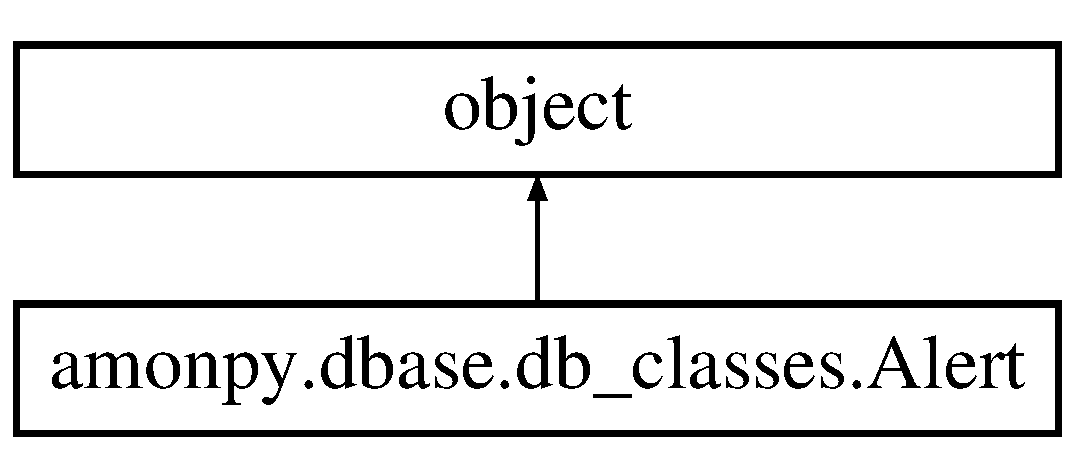
\includegraphics[height=2.000000cm]{classamonpy_1_1dbase_1_1db__classes_1_1_alert}
\end{center}
\end{figure}
\subsection*{Public Member Functions}
\begin{DoxyCompactItemize}
\item 
def \hyperlink{classamonpy_1_1dbase_1_1db__classes_1_1_alert_a50431e4196730d79202edbf8254a0bb8}{\-\_\-\-\_\-init\-\_\-\-\_\-}
\item 
def \hyperlink{classamonpy_1_1dbase_1_1db__classes_1_1_alert_a476ccdad5f6aa02bc76665f8a95160a2}{\-\_\-\-\_\-del\-\_\-\-\_\-}
\item 
def \hyperlink{classamonpy_1_1dbase_1_1db__classes_1_1_alert_a29c8eebc5f01603bdba8469547c0940d}{forprint}
\end{DoxyCompactItemize}
\subsection*{Public Attributes}
\begin{DoxyCompactItemize}
\item 
\hyperlink{classamonpy_1_1dbase_1_1db__classes_1_1_alert_ac351cba0cc9faed58731140738d10232}{stream}
\item 
\hyperlink{classamonpy_1_1dbase_1_1db__classes_1_1_alert_a3fbd21dde44ba9a6900e7c705fe1ac92}{id}
\item 
\hyperlink{classamonpy_1_1dbase_1_1db__classes_1_1_alert_aec0c9ca7bd4e69b38d501926ff93c259}{rev}
\item 
\hyperlink{classamonpy_1_1dbase_1_1db__classes_1_1_alert_ad2477bf8f38ef6e732880c14598934dc}{datetime}
\item 
\hyperlink{classamonpy_1_1dbase_1_1db__classes_1_1_alert_a5bf8ccdec5173b9ee4359fa1fe31827f}{R\-A}
\item 
\hyperlink{classamonpy_1_1dbase_1_1db__classes_1_1_alert_a971b1ce9cb028f39ad83c2aa8173385f}{dec}
\item 
\hyperlink{classamonpy_1_1dbase_1_1db__classes_1_1_alert_a87c586f9003da0f1fde613020fa94b6a}{sigma\-R}
\item 
\hyperlink{classamonpy_1_1dbase_1_1db__classes_1_1_alert_a315b616f084b56318fdd685fb73a7093}{nevents}
\item 
\hyperlink{classamonpy_1_1dbase_1_1db__classes_1_1_alert_ad8332cbb384c9623c60bc5ac2466dfcb}{delta\-T}
\item 
\hyperlink{classamonpy_1_1dbase_1_1db__classes_1_1_alert_a3cb6c2dbbacf6b0abb2ccfc04f9c8b54}{sigma\-T}
\item 
\hyperlink{classamonpy_1_1dbase_1_1db__classes_1_1_alert_a905c3768330fdf5753654c6c39259bbb}{false\-\_\-pos}
\item 
\hyperlink{classamonpy_1_1dbase_1_1db__classes_1_1_alert_a4734419472d0ed5c05acbd74f8a1ea63}{observing}
\item 
\hyperlink{classamonpy_1_1dbase_1_1db__classes_1_1_alert_ae7cb911f5a8c43290bc5f7263abbcfb0}{trigger}
\item 
\hyperlink{classamonpy_1_1dbase_1_1db__classes_1_1_alert_aab97b4bd290097eba5b8df6ca82a484d}{type}
\item 
\hyperlink{classamonpy_1_1dbase_1_1db__classes_1_1_alert_a4022fe5b40d0625fc2e97b2f4ee09a44}{pvalue}
\item 
\hyperlink{classamonpy_1_1dbase_1_1db__classes_1_1_alert_aa1a842a15827d212233963ceea89fb0c}{skymap}
\item 
\hyperlink{classamonpy_1_1dbase_1_1db__classes_1_1_alert_ae9e6b4386e95cb1a8f9c911b8dece0f6}{anarev}
\end{DoxyCompactItemize}
\subsection*{Static Public Attributes}
\begin{DoxyCompactItemize}
\item 
int \hyperlink{classamonpy_1_1dbase_1_1db__classes_1_1_alert_a57cb88bfad7b53e94ede6ac06de3ab46}{num\-\_\-alerts} = 0
\end{DoxyCompactItemize}


\subsection{Detailed Description}
\begin{DoxyVerb}Creates the Alert class. Instances are created by specifying a unique 
    triple of IDs (stream, id, rev). The other data attributes are set to
    defaults on init. This style may later be replaced by the class
    factory and __slots__ approach, currently adopted for the Event
    class (see above). However since Alerts are uncommon, they do not
    require the same level of optimization. 
\end{DoxyVerb}
 

\subsection{Constructor \& Destructor Documentation}
\hypertarget{classamonpy_1_1dbase_1_1db__classes_1_1_alert_a50431e4196730d79202edbf8254a0bb8}{\index{amonpy\-::dbase\-::db\-\_\-classes\-::\-Alert@{amonpy\-::dbase\-::db\-\_\-classes\-::\-Alert}!\-\_\-\-\_\-init\-\_\-\-\_\-@{\-\_\-\-\_\-init\-\_\-\-\_\-}}
\index{\-\_\-\-\_\-init\-\_\-\-\_\-@{\-\_\-\-\_\-init\-\_\-\-\_\-}!amonpy::dbase::db_classes::Alert@{amonpy\-::dbase\-::db\-\_\-classes\-::\-Alert}}
\subsubsection[{\-\_\-\-\_\-init\-\_\-\-\_\-}]{\setlength{\rightskip}{0pt plus 5cm}def amonpy.\-dbase.\-db\-\_\-classes.\-Alert.\-\_\-\-\_\-init\-\_\-\-\_\- (
\begin{DoxyParamCaption}
\item[{}]{self, }
\item[{}]{stream, }
\item[{}]{id, }
\item[{}]{rev}
\end{DoxyParamCaption}
)}}\label{classamonpy_1_1dbase_1_1db__classes_1_1_alert_a50431e4196730d79202edbf8254a0bb8}
\hypertarget{classamonpy_1_1dbase_1_1db__classes_1_1_alert_a476ccdad5f6aa02bc76665f8a95160a2}{\index{amonpy\-::dbase\-::db\-\_\-classes\-::\-Alert@{amonpy\-::dbase\-::db\-\_\-classes\-::\-Alert}!\-\_\-\-\_\-del\-\_\-\-\_\-@{\-\_\-\-\_\-del\-\_\-\-\_\-}}
\index{\-\_\-\-\_\-del\-\_\-\-\_\-@{\-\_\-\-\_\-del\-\_\-\-\_\-}!amonpy::dbase::db_classes::Alert@{amonpy\-::dbase\-::db\-\_\-classes\-::\-Alert}}
\subsubsection[{\-\_\-\-\_\-del\-\_\-\-\_\-}]{\setlength{\rightskip}{0pt plus 5cm}def amonpy.\-dbase.\-db\-\_\-classes.\-Alert.\-\_\-\-\_\-del\-\_\-\-\_\- (
\begin{DoxyParamCaption}
\item[{}]{self}
\end{DoxyParamCaption}
)}}\label{classamonpy_1_1dbase_1_1db__classes_1_1_alert_a476ccdad5f6aa02bc76665f8a95160a2}


\subsection{Member Function Documentation}
\hypertarget{classamonpy_1_1dbase_1_1db__classes_1_1_alert_a29c8eebc5f01603bdba8469547c0940d}{\index{amonpy\-::dbase\-::db\-\_\-classes\-::\-Alert@{amonpy\-::dbase\-::db\-\_\-classes\-::\-Alert}!forprint@{forprint}}
\index{forprint@{forprint}!amonpy::dbase::db_classes::Alert@{amonpy\-::dbase\-::db\-\_\-classes\-::\-Alert}}
\subsubsection[{forprint}]{\setlength{\rightskip}{0pt plus 5cm}def amonpy.\-dbase.\-db\-\_\-classes.\-Alert.\-forprint (
\begin{DoxyParamCaption}
\item[{}]{self}
\end{DoxyParamCaption}
)}}\label{classamonpy_1_1dbase_1_1db__classes_1_1_alert_a29c8eebc5f01603bdba8469547c0940d}


\subsection{Member Data Documentation}
\hypertarget{classamonpy_1_1dbase_1_1db__classes_1_1_alert_ae9e6b4386e95cb1a8f9c911b8dece0f6}{\index{amonpy\-::dbase\-::db\-\_\-classes\-::\-Alert@{amonpy\-::dbase\-::db\-\_\-classes\-::\-Alert}!anarev@{anarev}}
\index{anarev@{anarev}!amonpy::dbase::db_classes::Alert@{amonpy\-::dbase\-::db\-\_\-classes\-::\-Alert}}
\subsubsection[{anarev}]{\setlength{\rightskip}{0pt plus 5cm}amonpy.\-dbase.\-db\-\_\-classes.\-Alert.\-anarev}}\label{classamonpy_1_1dbase_1_1db__classes_1_1_alert_ae9e6b4386e95cb1a8f9c911b8dece0f6}
\hypertarget{classamonpy_1_1dbase_1_1db__classes_1_1_alert_ad2477bf8f38ef6e732880c14598934dc}{\index{amonpy\-::dbase\-::db\-\_\-classes\-::\-Alert@{amonpy\-::dbase\-::db\-\_\-classes\-::\-Alert}!datetime@{datetime}}
\index{datetime@{datetime}!amonpy::dbase::db_classes::Alert@{amonpy\-::dbase\-::db\-\_\-classes\-::\-Alert}}
\subsubsection[{datetime}]{\setlength{\rightskip}{0pt plus 5cm}amonpy.\-dbase.\-db\-\_\-classes.\-Alert.\-datetime}}\label{classamonpy_1_1dbase_1_1db__classes_1_1_alert_ad2477bf8f38ef6e732880c14598934dc}
\hypertarget{classamonpy_1_1dbase_1_1db__classes_1_1_alert_a971b1ce9cb028f39ad83c2aa8173385f}{\index{amonpy\-::dbase\-::db\-\_\-classes\-::\-Alert@{amonpy\-::dbase\-::db\-\_\-classes\-::\-Alert}!dec@{dec}}
\index{dec@{dec}!amonpy::dbase::db_classes::Alert@{amonpy\-::dbase\-::db\-\_\-classes\-::\-Alert}}
\subsubsection[{dec}]{\setlength{\rightskip}{0pt plus 5cm}amonpy.\-dbase.\-db\-\_\-classes.\-Alert.\-dec}}\label{classamonpy_1_1dbase_1_1db__classes_1_1_alert_a971b1ce9cb028f39ad83c2aa8173385f}
\hypertarget{classamonpy_1_1dbase_1_1db__classes_1_1_alert_ad8332cbb384c9623c60bc5ac2466dfcb}{\index{amonpy\-::dbase\-::db\-\_\-classes\-::\-Alert@{amonpy\-::dbase\-::db\-\_\-classes\-::\-Alert}!delta\-T@{delta\-T}}
\index{delta\-T@{delta\-T}!amonpy::dbase::db_classes::Alert@{amonpy\-::dbase\-::db\-\_\-classes\-::\-Alert}}
\subsubsection[{delta\-T}]{\setlength{\rightskip}{0pt plus 5cm}amonpy.\-dbase.\-db\-\_\-classes.\-Alert.\-delta\-T}}\label{classamonpy_1_1dbase_1_1db__classes_1_1_alert_ad8332cbb384c9623c60bc5ac2466dfcb}
\hypertarget{classamonpy_1_1dbase_1_1db__classes_1_1_alert_a905c3768330fdf5753654c6c39259bbb}{\index{amonpy\-::dbase\-::db\-\_\-classes\-::\-Alert@{amonpy\-::dbase\-::db\-\_\-classes\-::\-Alert}!false\-\_\-pos@{false\-\_\-pos}}
\index{false\-\_\-pos@{false\-\_\-pos}!amonpy::dbase::db_classes::Alert@{amonpy\-::dbase\-::db\-\_\-classes\-::\-Alert}}
\subsubsection[{false\-\_\-pos}]{\setlength{\rightskip}{0pt plus 5cm}amonpy.\-dbase.\-db\-\_\-classes.\-Alert.\-false\-\_\-pos}}\label{classamonpy_1_1dbase_1_1db__classes_1_1_alert_a905c3768330fdf5753654c6c39259bbb}
\hypertarget{classamonpy_1_1dbase_1_1db__classes_1_1_alert_a3fbd21dde44ba9a6900e7c705fe1ac92}{\index{amonpy\-::dbase\-::db\-\_\-classes\-::\-Alert@{amonpy\-::dbase\-::db\-\_\-classes\-::\-Alert}!id@{id}}
\index{id@{id}!amonpy::dbase::db_classes::Alert@{amonpy\-::dbase\-::db\-\_\-classes\-::\-Alert}}
\subsubsection[{id}]{\setlength{\rightskip}{0pt plus 5cm}amonpy.\-dbase.\-db\-\_\-classes.\-Alert.\-id}}\label{classamonpy_1_1dbase_1_1db__classes_1_1_alert_a3fbd21dde44ba9a6900e7c705fe1ac92}
\hypertarget{classamonpy_1_1dbase_1_1db__classes_1_1_alert_a315b616f084b56318fdd685fb73a7093}{\index{amonpy\-::dbase\-::db\-\_\-classes\-::\-Alert@{amonpy\-::dbase\-::db\-\_\-classes\-::\-Alert}!nevents@{nevents}}
\index{nevents@{nevents}!amonpy::dbase::db_classes::Alert@{amonpy\-::dbase\-::db\-\_\-classes\-::\-Alert}}
\subsubsection[{nevents}]{\setlength{\rightskip}{0pt plus 5cm}amonpy.\-dbase.\-db\-\_\-classes.\-Alert.\-nevents}}\label{classamonpy_1_1dbase_1_1db__classes_1_1_alert_a315b616f084b56318fdd685fb73a7093}
\hypertarget{classamonpy_1_1dbase_1_1db__classes_1_1_alert_a57cb88bfad7b53e94ede6ac06de3ab46}{\index{amonpy\-::dbase\-::db\-\_\-classes\-::\-Alert@{amonpy\-::dbase\-::db\-\_\-classes\-::\-Alert}!num\-\_\-alerts@{num\-\_\-alerts}}
\index{num\-\_\-alerts@{num\-\_\-alerts}!amonpy::dbase::db_classes::Alert@{amonpy\-::dbase\-::db\-\_\-classes\-::\-Alert}}
\subsubsection[{num\-\_\-alerts}]{\setlength{\rightskip}{0pt plus 5cm}int amonpy.\-dbase.\-db\-\_\-classes.\-Alert.\-num\-\_\-alerts = 0\hspace{0.3cm}{\ttfamily [static]}}}\label{classamonpy_1_1dbase_1_1db__classes_1_1_alert_a57cb88bfad7b53e94ede6ac06de3ab46}
\hypertarget{classamonpy_1_1dbase_1_1db__classes_1_1_alert_a4734419472d0ed5c05acbd74f8a1ea63}{\index{amonpy\-::dbase\-::db\-\_\-classes\-::\-Alert@{amonpy\-::dbase\-::db\-\_\-classes\-::\-Alert}!observing@{observing}}
\index{observing@{observing}!amonpy::dbase::db_classes::Alert@{amonpy\-::dbase\-::db\-\_\-classes\-::\-Alert}}
\subsubsection[{observing}]{\setlength{\rightskip}{0pt plus 5cm}amonpy.\-dbase.\-db\-\_\-classes.\-Alert.\-observing}}\label{classamonpy_1_1dbase_1_1db__classes_1_1_alert_a4734419472d0ed5c05acbd74f8a1ea63}
\hypertarget{classamonpy_1_1dbase_1_1db__classes_1_1_alert_a4022fe5b40d0625fc2e97b2f4ee09a44}{\index{amonpy\-::dbase\-::db\-\_\-classes\-::\-Alert@{amonpy\-::dbase\-::db\-\_\-classes\-::\-Alert}!pvalue@{pvalue}}
\index{pvalue@{pvalue}!amonpy::dbase::db_classes::Alert@{amonpy\-::dbase\-::db\-\_\-classes\-::\-Alert}}
\subsubsection[{pvalue}]{\setlength{\rightskip}{0pt plus 5cm}amonpy.\-dbase.\-db\-\_\-classes.\-Alert.\-pvalue}}\label{classamonpy_1_1dbase_1_1db__classes_1_1_alert_a4022fe5b40d0625fc2e97b2f4ee09a44}
\hypertarget{classamonpy_1_1dbase_1_1db__classes_1_1_alert_a5bf8ccdec5173b9ee4359fa1fe31827f}{\index{amonpy\-::dbase\-::db\-\_\-classes\-::\-Alert@{amonpy\-::dbase\-::db\-\_\-classes\-::\-Alert}!R\-A@{R\-A}}
\index{R\-A@{R\-A}!amonpy::dbase::db_classes::Alert@{amonpy\-::dbase\-::db\-\_\-classes\-::\-Alert}}
\subsubsection[{R\-A}]{\setlength{\rightskip}{0pt plus 5cm}amonpy.\-dbase.\-db\-\_\-classes.\-Alert.\-R\-A}}\label{classamonpy_1_1dbase_1_1db__classes_1_1_alert_a5bf8ccdec5173b9ee4359fa1fe31827f}
\hypertarget{classamonpy_1_1dbase_1_1db__classes_1_1_alert_aec0c9ca7bd4e69b38d501926ff93c259}{\index{amonpy\-::dbase\-::db\-\_\-classes\-::\-Alert@{amonpy\-::dbase\-::db\-\_\-classes\-::\-Alert}!rev@{rev}}
\index{rev@{rev}!amonpy::dbase::db_classes::Alert@{amonpy\-::dbase\-::db\-\_\-classes\-::\-Alert}}
\subsubsection[{rev}]{\setlength{\rightskip}{0pt plus 5cm}amonpy.\-dbase.\-db\-\_\-classes.\-Alert.\-rev}}\label{classamonpy_1_1dbase_1_1db__classes_1_1_alert_aec0c9ca7bd4e69b38d501926ff93c259}
\hypertarget{classamonpy_1_1dbase_1_1db__classes_1_1_alert_a87c586f9003da0f1fde613020fa94b6a}{\index{amonpy\-::dbase\-::db\-\_\-classes\-::\-Alert@{amonpy\-::dbase\-::db\-\_\-classes\-::\-Alert}!sigma\-R@{sigma\-R}}
\index{sigma\-R@{sigma\-R}!amonpy::dbase::db_classes::Alert@{amonpy\-::dbase\-::db\-\_\-classes\-::\-Alert}}
\subsubsection[{sigma\-R}]{\setlength{\rightskip}{0pt plus 5cm}amonpy.\-dbase.\-db\-\_\-classes.\-Alert.\-sigma\-R}}\label{classamonpy_1_1dbase_1_1db__classes_1_1_alert_a87c586f9003da0f1fde613020fa94b6a}
\hypertarget{classamonpy_1_1dbase_1_1db__classes_1_1_alert_a3cb6c2dbbacf6b0abb2ccfc04f9c8b54}{\index{amonpy\-::dbase\-::db\-\_\-classes\-::\-Alert@{amonpy\-::dbase\-::db\-\_\-classes\-::\-Alert}!sigma\-T@{sigma\-T}}
\index{sigma\-T@{sigma\-T}!amonpy::dbase::db_classes::Alert@{amonpy\-::dbase\-::db\-\_\-classes\-::\-Alert}}
\subsubsection[{sigma\-T}]{\setlength{\rightskip}{0pt plus 5cm}amonpy.\-dbase.\-db\-\_\-classes.\-Alert.\-sigma\-T}}\label{classamonpy_1_1dbase_1_1db__classes_1_1_alert_a3cb6c2dbbacf6b0abb2ccfc04f9c8b54}
\hypertarget{classamonpy_1_1dbase_1_1db__classes_1_1_alert_aa1a842a15827d212233963ceea89fb0c}{\index{amonpy\-::dbase\-::db\-\_\-classes\-::\-Alert@{amonpy\-::dbase\-::db\-\_\-classes\-::\-Alert}!skymap@{skymap}}
\index{skymap@{skymap}!amonpy::dbase::db_classes::Alert@{amonpy\-::dbase\-::db\-\_\-classes\-::\-Alert}}
\subsubsection[{skymap}]{\setlength{\rightskip}{0pt plus 5cm}amonpy.\-dbase.\-db\-\_\-classes.\-Alert.\-skymap}}\label{classamonpy_1_1dbase_1_1db__classes_1_1_alert_aa1a842a15827d212233963ceea89fb0c}
\hypertarget{classamonpy_1_1dbase_1_1db__classes_1_1_alert_ac351cba0cc9faed58731140738d10232}{\index{amonpy\-::dbase\-::db\-\_\-classes\-::\-Alert@{amonpy\-::dbase\-::db\-\_\-classes\-::\-Alert}!stream@{stream}}
\index{stream@{stream}!amonpy::dbase::db_classes::Alert@{amonpy\-::dbase\-::db\-\_\-classes\-::\-Alert}}
\subsubsection[{stream}]{\setlength{\rightskip}{0pt plus 5cm}amonpy.\-dbase.\-db\-\_\-classes.\-Alert.\-stream}}\label{classamonpy_1_1dbase_1_1db__classes_1_1_alert_ac351cba0cc9faed58731140738d10232}
\hypertarget{classamonpy_1_1dbase_1_1db__classes_1_1_alert_ae7cb911f5a8c43290bc5f7263abbcfb0}{\index{amonpy\-::dbase\-::db\-\_\-classes\-::\-Alert@{amonpy\-::dbase\-::db\-\_\-classes\-::\-Alert}!trigger@{trigger}}
\index{trigger@{trigger}!amonpy::dbase::db_classes::Alert@{amonpy\-::dbase\-::db\-\_\-classes\-::\-Alert}}
\subsubsection[{trigger}]{\setlength{\rightskip}{0pt plus 5cm}amonpy.\-dbase.\-db\-\_\-classes.\-Alert.\-trigger}}\label{classamonpy_1_1dbase_1_1db__classes_1_1_alert_ae7cb911f5a8c43290bc5f7263abbcfb0}
\hypertarget{classamonpy_1_1dbase_1_1db__classes_1_1_alert_aab97b4bd290097eba5b8df6ca82a484d}{\index{amonpy\-::dbase\-::db\-\_\-classes\-::\-Alert@{amonpy\-::dbase\-::db\-\_\-classes\-::\-Alert}!type@{type}}
\index{type@{type}!amonpy::dbase::db_classes::Alert@{amonpy\-::dbase\-::db\-\_\-classes\-::\-Alert}}
\subsubsection[{type}]{\setlength{\rightskip}{0pt plus 5cm}amonpy.\-dbase.\-db\-\_\-classes.\-Alert.\-type}}\label{classamonpy_1_1dbase_1_1db__classes_1_1_alert_aab97b4bd290097eba5b8df6ca82a484d}


The documentation for this class was generated from the following file\-:\begin{DoxyCompactItemize}
\item 
amonpy/dbase/\hyperlink{db__classes_8py}{db\-\_\-classes.\-py}\end{DoxyCompactItemize}

\hypertarget{classamonpy_1_1dbase_1_1db__classes_1_1_alert_config}{\section{amonpy.\-dbase.\-db\-\_\-classes.\-Alert\-Config Class Reference}
\label{classamonpy_1_1dbase_1_1db__classes_1_1_alert_config}\index{amonpy.\-dbase.\-db\-\_\-classes.\-Alert\-Config@{amonpy.\-dbase.\-db\-\_\-classes.\-Alert\-Config}}
}


Creates the \hyperlink{classamonpy_1_1dbase_1_1db__classes_1_1_alert_config}{Alert\-Config} class.  


Inheritance diagram for amonpy.\-dbase.\-db\-\_\-classes.\-Alert\-Config\-:\begin{figure}[H]
\begin{center}
\leavevmode
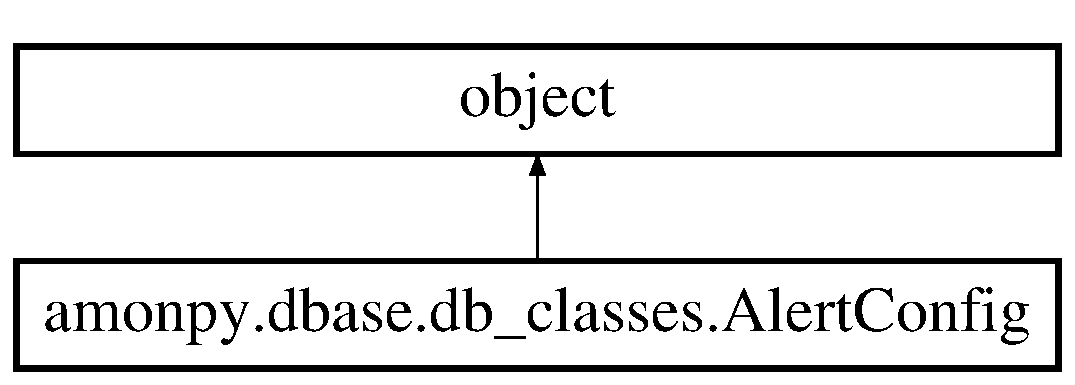
\includegraphics[height=2.000000cm]{d1/d62/classamonpy_1_1dbase_1_1db__classes_1_1_alert_config}
\end{center}
\end{figure}
\subsection*{Public Member Functions}
\begin{DoxyCompactItemize}
\item 
def \hyperlink{classamonpy_1_1dbase_1_1db__classes_1_1_alert_config_ac579b972a4ff6bbd4770a04df3bcb744}{\-\_\-\-\_\-init\-\_\-\-\_\-}
\item 
def \hyperlink{classamonpy_1_1dbase_1_1db__classes_1_1_alert_config_a0b505c28e0b2083d929998465a3d205c}{\-\_\-\-\_\-del\-\_\-\-\_\-}
\item 
def \hyperlink{classamonpy_1_1dbase_1_1db__classes_1_1_alert_config_a4199bb054162725442056137dac9c760}{forprint}
\end{DoxyCompactItemize}
\subsection*{Public Attributes}
\begin{DoxyCompactItemize}
\item 
\hyperlink{classamonpy_1_1dbase_1_1db__classes_1_1_alert_config_a5181b25cd2b3960297851cac7538eeb5}{stream}
\item 
\hyperlink{classamonpy_1_1dbase_1_1db__classes_1_1_alert_config_a73ac175f4751ace5efefa98ccbfc0785}{rev}
\item 
\hyperlink{classamonpy_1_1dbase_1_1db__classes_1_1_alert_config_ac4d6388204f392c5838eb2902a5cf263}{valid\-Start}
\item 
\hyperlink{classamonpy_1_1dbase_1_1db__classes_1_1_alert_config_af8bb43caa61b4c962ea2e96dc8722461}{valid\-Stop}
\item 
\hyperlink{classamonpy_1_1dbase_1_1db__classes_1_1_alert_config_a39184be5dae1af25cad32181fbe17c61}{participating}
\item 
\hyperlink{classamonpy_1_1dbase_1_1db__classes_1_1_alert_config_a16d50003ae8ad8876cc0a7cb283c6968}{p\-\_\-thresh}
\item 
\hyperlink{classamonpy_1_1dbase_1_1db__classes_1_1_alert_config_aec4a19cdc1a4fa7269378278fe36bce3}{N\-\_\-thresh}
\item 
\hyperlink{classamonpy_1_1dbase_1_1db__classes_1_1_alert_config_ae6ec661f2f82ef7d84f6285a6feacaa9}{delta\-T}
\item 
\hyperlink{classamonpy_1_1dbase_1_1db__classes_1_1_alert_config_aeb4dd54c70c114a00192659ba9881a9b}{cluster\-\_\-method}
\item 
\hyperlink{classamonpy_1_1dbase_1_1db__classes_1_1_alert_config_acfdfd05a7551c6ee13a4c04970a5b496}{sens\-\_\-thresh}
\item 
\hyperlink{classamonpy_1_1dbase_1_1db__classes_1_1_alert_config_a73eaa3edce9df7437c2f385e5ffcdc27}{skymap\-\_\-val1\-Desc}
\item 
\hyperlink{classamonpy_1_1dbase_1_1db__classes_1_1_alert_config_ad123a3f944545c402b09637d5fd3068a}{skymap\-\_\-val2\-Desc}
\item 
\hyperlink{classamonpy_1_1dbase_1_1db__classes_1_1_alert_config_a5150e8d288983b9436a2d356c33537cc}{skymap\-\_\-val3\-Desc}
\item 
\hyperlink{classamonpy_1_1dbase_1_1db__classes_1_1_alert_config_af0aff8769055be290414b5bd6364d180}{buffer\-T}
\item 
\hyperlink{classamonpy_1_1dbase_1_1db__classes_1_1_alert_config_aaede4885574230fc56b90fc989230a85}{R\-\_\-thresh}
\item 
\hyperlink{classamonpy_1_1dbase_1_1db__classes_1_1_alert_config_ac3cf39c10bcacbd6209f3175788168f6}{cluster\-\_\-thresh}
\end{DoxyCompactItemize}
\subsection*{Static Public Attributes}
\begin{DoxyCompactItemize}
\item 
int \hyperlink{classamonpy_1_1dbase_1_1db__classes_1_1_alert_config_ad02d71bf530446fdd3e8e87fb82bafb8}{num\-\_\-configs} = 0
\end{DoxyCompactItemize}


\subsection{Detailed Description}
Creates the \hyperlink{classamonpy_1_1dbase_1_1db__classes_1_1_alert_config}{Alert\-Config} class. 

Instances are created by specifying a unique double of I\-Ds (stream, rev). This version is retained for the purposes of testing database read/write of the corresponding table. 

Definition at line 434 of file db\-\_\-classes.\-py.



\subsection{Constructor \& Destructor Documentation}
\hypertarget{classamonpy_1_1dbase_1_1db__classes_1_1_alert_config_ac579b972a4ff6bbd4770a04df3bcb744}{\index{amonpy\-::dbase\-::db\-\_\-classes\-::\-Alert\-Config@{amonpy\-::dbase\-::db\-\_\-classes\-::\-Alert\-Config}!\-\_\-\-\_\-init\-\_\-\-\_\-@{\-\_\-\-\_\-init\-\_\-\-\_\-}}
\index{\-\_\-\-\_\-init\-\_\-\-\_\-@{\-\_\-\-\_\-init\-\_\-\-\_\-}!amonpy::dbase::db_classes::AlertConfig@{amonpy\-::dbase\-::db\-\_\-classes\-::\-Alert\-Config}}
\subsubsection[{\-\_\-\-\_\-init\-\_\-\-\_\-}]{\setlength{\rightskip}{0pt plus 5cm}def amonpy.\-dbase.\-db\-\_\-classes.\-Alert\-Config.\-\_\-\-\_\-init\-\_\-\-\_\- (
\begin{DoxyParamCaption}
\item[{}]{self, }
\item[{}]{stream, }
\item[{}]{rev}
\end{DoxyParamCaption}
)}}\label{classamonpy_1_1dbase_1_1db__classes_1_1_alert_config_ac579b972a4ff6bbd4770a04df3bcb744}


Definition at line 436 of file db\-\_\-classes.\-py.

\hypertarget{classamonpy_1_1dbase_1_1db__classes_1_1_alert_config_a0b505c28e0b2083d929998465a3d205c}{\index{amonpy\-::dbase\-::db\-\_\-classes\-::\-Alert\-Config@{amonpy\-::dbase\-::db\-\_\-classes\-::\-Alert\-Config}!\-\_\-\-\_\-del\-\_\-\-\_\-@{\-\_\-\-\_\-del\-\_\-\-\_\-}}
\index{\-\_\-\-\_\-del\-\_\-\-\_\-@{\-\_\-\-\_\-del\-\_\-\-\_\-}!amonpy::dbase::db_classes::AlertConfig@{amonpy\-::dbase\-::db\-\_\-classes\-::\-Alert\-Config}}
\subsubsection[{\-\_\-\-\_\-del\-\_\-\-\_\-}]{\setlength{\rightskip}{0pt plus 5cm}def amonpy.\-dbase.\-db\-\_\-classes.\-Alert\-Config.\-\_\-\-\_\-del\-\_\-\-\_\- (
\begin{DoxyParamCaption}
\item[{}]{self}
\end{DoxyParamCaption}
)}}\label{classamonpy_1_1dbase_1_1db__classes_1_1_alert_config_a0b505c28e0b2083d929998465a3d205c}


Definition at line 454 of file db\-\_\-classes.\-py.



\subsection{Member Function Documentation}
\hypertarget{classamonpy_1_1dbase_1_1db__classes_1_1_alert_config_a4199bb054162725442056137dac9c760}{\index{amonpy\-::dbase\-::db\-\_\-classes\-::\-Alert\-Config@{amonpy\-::dbase\-::db\-\_\-classes\-::\-Alert\-Config}!forprint@{forprint}}
\index{forprint@{forprint}!amonpy::dbase::db_classes::AlertConfig@{amonpy\-::dbase\-::db\-\_\-classes\-::\-Alert\-Config}}
\subsubsection[{forprint}]{\setlength{\rightskip}{0pt plus 5cm}def amonpy.\-dbase.\-db\-\_\-classes.\-Alert\-Config.\-forprint (
\begin{DoxyParamCaption}
\item[{}]{self}
\end{DoxyParamCaption}
)}}\label{classamonpy_1_1dbase_1_1db__classes_1_1_alert_config_a4199bb054162725442056137dac9c760}


Definition at line 457 of file db\-\_\-classes.\-py.



\subsection{Member Data Documentation}
\hypertarget{classamonpy_1_1dbase_1_1db__classes_1_1_alert_config_af0aff8769055be290414b5bd6364d180}{\index{amonpy\-::dbase\-::db\-\_\-classes\-::\-Alert\-Config@{amonpy\-::dbase\-::db\-\_\-classes\-::\-Alert\-Config}!buffer\-T@{buffer\-T}}
\index{buffer\-T@{buffer\-T}!amonpy::dbase::db_classes::AlertConfig@{amonpy\-::dbase\-::db\-\_\-classes\-::\-Alert\-Config}}
\subsubsection[{buffer\-T}]{\setlength{\rightskip}{0pt plus 5cm}amonpy.\-dbase.\-db\-\_\-classes.\-Alert\-Config.\-buffer\-T}}\label{classamonpy_1_1dbase_1_1db__classes_1_1_alert_config_af0aff8769055be290414b5bd6364d180}


Definition at line 450 of file db\-\_\-classes.\-py.

\hypertarget{classamonpy_1_1dbase_1_1db__classes_1_1_alert_config_aeb4dd54c70c114a00192659ba9881a9b}{\index{amonpy\-::dbase\-::db\-\_\-classes\-::\-Alert\-Config@{amonpy\-::dbase\-::db\-\_\-classes\-::\-Alert\-Config}!cluster\-\_\-method@{cluster\-\_\-method}}
\index{cluster\-\_\-method@{cluster\-\_\-method}!amonpy::dbase::db_classes::AlertConfig@{amonpy\-::dbase\-::db\-\_\-classes\-::\-Alert\-Config}}
\subsubsection[{cluster\-\_\-method}]{\setlength{\rightskip}{0pt plus 5cm}amonpy.\-dbase.\-db\-\_\-classes.\-Alert\-Config.\-cluster\-\_\-method}}\label{classamonpy_1_1dbase_1_1db__classes_1_1_alert_config_aeb4dd54c70c114a00192659ba9881a9b}


Definition at line 445 of file db\-\_\-classes.\-py.

\hypertarget{classamonpy_1_1dbase_1_1db__classes_1_1_alert_config_ac3cf39c10bcacbd6209f3175788168f6}{\index{amonpy\-::dbase\-::db\-\_\-classes\-::\-Alert\-Config@{amonpy\-::dbase\-::db\-\_\-classes\-::\-Alert\-Config}!cluster\-\_\-thresh@{cluster\-\_\-thresh}}
\index{cluster\-\_\-thresh@{cluster\-\_\-thresh}!amonpy::dbase::db_classes::AlertConfig@{amonpy\-::dbase\-::db\-\_\-classes\-::\-Alert\-Config}}
\subsubsection[{cluster\-\_\-thresh}]{\setlength{\rightskip}{0pt plus 5cm}amonpy.\-dbase.\-db\-\_\-classes.\-Alert\-Config.\-cluster\-\_\-thresh}}\label{classamonpy_1_1dbase_1_1db__classes_1_1_alert_config_ac3cf39c10bcacbd6209f3175788168f6}


Definition at line 452 of file db\-\_\-classes.\-py.

\hypertarget{classamonpy_1_1dbase_1_1db__classes_1_1_alert_config_ae6ec661f2f82ef7d84f6285a6feacaa9}{\index{amonpy\-::dbase\-::db\-\_\-classes\-::\-Alert\-Config@{amonpy\-::dbase\-::db\-\_\-classes\-::\-Alert\-Config}!delta\-T@{delta\-T}}
\index{delta\-T@{delta\-T}!amonpy::dbase::db_classes::AlertConfig@{amonpy\-::dbase\-::db\-\_\-classes\-::\-Alert\-Config}}
\subsubsection[{delta\-T}]{\setlength{\rightskip}{0pt plus 5cm}amonpy.\-dbase.\-db\-\_\-classes.\-Alert\-Config.\-delta\-T}}\label{classamonpy_1_1dbase_1_1db__classes_1_1_alert_config_ae6ec661f2f82ef7d84f6285a6feacaa9}


Definition at line 444 of file db\-\_\-classes.\-py.

\hypertarget{classamonpy_1_1dbase_1_1db__classes_1_1_alert_config_aec4a19cdc1a4fa7269378278fe36bce3}{\index{amonpy\-::dbase\-::db\-\_\-classes\-::\-Alert\-Config@{amonpy\-::dbase\-::db\-\_\-classes\-::\-Alert\-Config}!N\-\_\-thresh@{N\-\_\-thresh}}
\index{N\-\_\-thresh@{N\-\_\-thresh}!amonpy::dbase::db_classes::AlertConfig@{amonpy\-::dbase\-::db\-\_\-classes\-::\-Alert\-Config}}
\subsubsection[{N\-\_\-thresh}]{\setlength{\rightskip}{0pt plus 5cm}amonpy.\-dbase.\-db\-\_\-classes.\-Alert\-Config.\-N\-\_\-thresh}}\label{classamonpy_1_1dbase_1_1db__classes_1_1_alert_config_aec4a19cdc1a4fa7269378278fe36bce3}


Definition at line 443 of file db\-\_\-classes.\-py.

\hypertarget{classamonpy_1_1dbase_1_1db__classes_1_1_alert_config_ad02d71bf530446fdd3e8e87fb82bafb8}{\index{amonpy\-::dbase\-::db\-\_\-classes\-::\-Alert\-Config@{amonpy\-::dbase\-::db\-\_\-classes\-::\-Alert\-Config}!num\-\_\-configs@{num\-\_\-configs}}
\index{num\-\_\-configs@{num\-\_\-configs}!amonpy::dbase::db_classes::AlertConfig@{amonpy\-::dbase\-::db\-\_\-classes\-::\-Alert\-Config}}
\subsubsection[{num\-\_\-configs}]{\setlength{\rightskip}{0pt plus 5cm}int amonpy.\-dbase.\-db\-\_\-classes.\-Alert\-Config.\-num\-\_\-configs = 0\hspace{0.3cm}{\ttfamily [static]}}}\label{classamonpy_1_1dbase_1_1db__classes_1_1_alert_config_ad02d71bf530446fdd3e8e87fb82bafb8}


Definition at line 435 of file db\-\_\-classes.\-py.

\hypertarget{classamonpy_1_1dbase_1_1db__classes_1_1_alert_config_a16d50003ae8ad8876cc0a7cb283c6968}{\index{amonpy\-::dbase\-::db\-\_\-classes\-::\-Alert\-Config@{amonpy\-::dbase\-::db\-\_\-classes\-::\-Alert\-Config}!p\-\_\-thresh@{p\-\_\-thresh}}
\index{p\-\_\-thresh@{p\-\_\-thresh}!amonpy::dbase::db_classes::AlertConfig@{amonpy\-::dbase\-::db\-\_\-classes\-::\-Alert\-Config}}
\subsubsection[{p\-\_\-thresh}]{\setlength{\rightskip}{0pt plus 5cm}amonpy.\-dbase.\-db\-\_\-classes.\-Alert\-Config.\-p\-\_\-thresh}}\label{classamonpy_1_1dbase_1_1db__classes_1_1_alert_config_a16d50003ae8ad8876cc0a7cb283c6968}


Definition at line 442 of file db\-\_\-classes.\-py.

\hypertarget{classamonpy_1_1dbase_1_1db__classes_1_1_alert_config_a39184be5dae1af25cad32181fbe17c61}{\index{amonpy\-::dbase\-::db\-\_\-classes\-::\-Alert\-Config@{amonpy\-::dbase\-::db\-\_\-classes\-::\-Alert\-Config}!participating@{participating}}
\index{participating@{participating}!amonpy::dbase::db_classes::AlertConfig@{amonpy\-::dbase\-::db\-\_\-classes\-::\-Alert\-Config}}
\subsubsection[{participating}]{\setlength{\rightskip}{0pt plus 5cm}amonpy.\-dbase.\-db\-\_\-classes.\-Alert\-Config.\-participating}}\label{classamonpy_1_1dbase_1_1db__classes_1_1_alert_config_a39184be5dae1af25cad32181fbe17c61}


Definition at line 441 of file db\-\_\-classes.\-py.

\hypertarget{classamonpy_1_1dbase_1_1db__classes_1_1_alert_config_aaede4885574230fc56b90fc989230a85}{\index{amonpy\-::dbase\-::db\-\_\-classes\-::\-Alert\-Config@{amonpy\-::dbase\-::db\-\_\-classes\-::\-Alert\-Config}!R\-\_\-thresh@{R\-\_\-thresh}}
\index{R\-\_\-thresh@{R\-\_\-thresh}!amonpy::dbase::db_classes::AlertConfig@{amonpy\-::dbase\-::db\-\_\-classes\-::\-Alert\-Config}}
\subsubsection[{R\-\_\-thresh}]{\setlength{\rightskip}{0pt plus 5cm}amonpy.\-dbase.\-db\-\_\-classes.\-Alert\-Config.\-R\-\_\-thresh}}\label{classamonpy_1_1dbase_1_1db__classes_1_1_alert_config_aaede4885574230fc56b90fc989230a85}


Definition at line 451 of file db\-\_\-classes.\-py.

\hypertarget{classamonpy_1_1dbase_1_1db__classes_1_1_alert_config_a73ac175f4751ace5efefa98ccbfc0785}{\index{amonpy\-::dbase\-::db\-\_\-classes\-::\-Alert\-Config@{amonpy\-::dbase\-::db\-\_\-classes\-::\-Alert\-Config}!rev@{rev}}
\index{rev@{rev}!amonpy::dbase::db_classes::AlertConfig@{amonpy\-::dbase\-::db\-\_\-classes\-::\-Alert\-Config}}
\subsubsection[{rev}]{\setlength{\rightskip}{0pt plus 5cm}amonpy.\-dbase.\-db\-\_\-classes.\-Alert\-Config.\-rev}}\label{classamonpy_1_1dbase_1_1db__classes_1_1_alert_config_a73ac175f4751ace5efefa98ccbfc0785}


Definition at line 438 of file db\-\_\-classes.\-py.

\hypertarget{classamonpy_1_1dbase_1_1db__classes_1_1_alert_config_acfdfd05a7551c6ee13a4c04970a5b496}{\index{amonpy\-::dbase\-::db\-\_\-classes\-::\-Alert\-Config@{amonpy\-::dbase\-::db\-\_\-classes\-::\-Alert\-Config}!sens\-\_\-thresh@{sens\-\_\-thresh}}
\index{sens\-\_\-thresh@{sens\-\_\-thresh}!amonpy::dbase::db_classes::AlertConfig@{amonpy\-::dbase\-::db\-\_\-classes\-::\-Alert\-Config}}
\subsubsection[{sens\-\_\-thresh}]{\setlength{\rightskip}{0pt plus 5cm}amonpy.\-dbase.\-db\-\_\-classes.\-Alert\-Config.\-sens\-\_\-thresh}}\label{classamonpy_1_1dbase_1_1db__classes_1_1_alert_config_acfdfd05a7551c6ee13a4c04970a5b496}


Definition at line 446 of file db\-\_\-classes.\-py.

\hypertarget{classamonpy_1_1dbase_1_1db__classes_1_1_alert_config_a73eaa3edce9df7437c2f385e5ffcdc27}{\index{amonpy\-::dbase\-::db\-\_\-classes\-::\-Alert\-Config@{amonpy\-::dbase\-::db\-\_\-classes\-::\-Alert\-Config}!skymap\-\_\-val1\-Desc@{skymap\-\_\-val1\-Desc}}
\index{skymap\-\_\-val1\-Desc@{skymap\-\_\-val1\-Desc}!amonpy::dbase::db_classes::AlertConfig@{amonpy\-::dbase\-::db\-\_\-classes\-::\-Alert\-Config}}
\subsubsection[{skymap\-\_\-val1\-Desc}]{\setlength{\rightskip}{0pt plus 5cm}amonpy.\-dbase.\-db\-\_\-classes.\-Alert\-Config.\-skymap\-\_\-val1\-Desc}}\label{classamonpy_1_1dbase_1_1db__classes_1_1_alert_config_a73eaa3edce9df7437c2f385e5ffcdc27}


Definition at line 447 of file db\-\_\-classes.\-py.

\hypertarget{classamonpy_1_1dbase_1_1db__classes_1_1_alert_config_ad123a3f944545c402b09637d5fd3068a}{\index{amonpy\-::dbase\-::db\-\_\-classes\-::\-Alert\-Config@{amonpy\-::dbase\-::db\-\_\-classes\-::\-Alert\-Config}!skymap\-\_\-val2\-Desc@{skymap\-\_\-val2\-Desc}}
\index{skymap\-\_\-val2\-Desc@{skymap\-\_\-val2\-Desc}!amonpy::dbase::db_classes::AlertConfig@{amonpy\-::dbase\-::db\-\_\-classes\-::\-Alert\-Config}}
\subsubsection[{skymap\-\_\-val2\-Desc}]{\setlength{\rightskip}{0pt plus 5cm}amonpy.\-dbase.\-db\-\_\-classes.\-Alert\-Config.\-skymap\-\_\-val2\-Desc}}\label{classamonpy_1_1dbase_1_1db__classes_1_1_alert_config_ad123a3f944545c402b09637d5fd3068a}


Definition at line 448 of file db\-\_\-classes.\-py.

\hypertarget{classamonpy_1_1dbase_1_1db__classes_1_1_alert_config_a5150e8d288983b9436a2d356c33537cc}{\index{amonpy\-::dbase\-::db\-\_\-classes\-::\-Alert\-Config@{amonpy\-::dbase\-::db\-\_\-classes\-::\-Alert\-Config}!skymap\-\_\-val3\-Desc@{skymap\-\_\-val3\-Desc}}
\index{skymap\-\_\-val3\-Desc@{skymap\-\_\-val3\-Desc}!amonpy::dbase::db_classes::AlertConfig@{amonpy\-::dbase\-::db\-\_\-classes\-::\-Alert\-Config}}
\subsubsection[{skymap\-\_\-val3\-Desc}]{\setlength{\rightskip}{0pt plus 5cm}amonpy.\-dbase.\-db\-\_\-classes.\-Alert\-Config.\-skymap\-\_\-val3\-Desc}}\label{classamonpy_1_1dbase_1_1db__classes_1_1_alert_config_a5150e8d288983b9436a2d356c33537cc}


Definition at line 449 of file db\-\_\-classes.\-py.

\hypertarget{classamonpy_1_1dbase_1_1db__classes_1_1_alert_config_a5181b25cd2b3960297851cac7538eeb5}{\index{amonpy\-::dbase\-::db\-\_\-classes\-::\-Alert\-Config@{amonpy\-::dbase\-::db\-\_\-classes\-::\-Alert\-Config}!stream@{stream}}
\index{stream@{stream}!amonpy::dbase::db_classes::AlertConfig@{amonpy\-::dbase\-::db\-\_\-classes\-::\-Alert\-Config}}
\subsubsection[{stream}]{\setlength{\rightskip}{0pt plus 5cm}amonpy.\-dbase.\-db\-\_\-classes.\-Alert\-Config.\-stream}}\label{classamonpy_1_1dbase_1_1db__classes_1_1_alert_config_a5181b25cd2b3960297851cac7538eeb5}


Definition at line 437 of file db\-\_\-classes.\-py.

\hypertarget{classamonpy_1_1dbase_1_1db__classes_1_1_alert_config_ac4d6388204f392c5838eb2902a5cf263}{\index{amonpy\-::dbase\-::db\-\_\-classes\-::\-Alert\-Config@{amonpy\-::dbase\-::db\-\_\-classes\-::\-Alert\-Config}!valid\-Start@{valid\-Start}}
\index{valid\-Start@{valid\-Start}!amonpy::dbase::db_classes::AlertConfig@{amonpy\-::dbase\-::db\-\_\-classes\-::\-Alert\-Config}}
\subsubsection[{valid\-Start}]{\setlength{\rightskip}{0pt plus 5cm}amonpy.\-dbase.\-db\-\_\-classes.\-Alert\-Config.\-valid\-Start}}\label{classamonpy_1_1dbase_1_1db__classes_1_1_alert_config_ac4d6388204f392c5838eb2902a5cf263}


Definition at line 439 of file db\-\_\-classes.\-py.

\hypertarget{classamonpy_1_1dbase_1_1db__classes_1_1_alert_config_af8bb43caa61b4c962ea2e96dc8722461}{\index{amonpy\-::dbase\-::db\-\_\-classes\-::\-Alert\-Config@{amonpy\-::dbase\-::db\-\_\-classes\-::\-Alert\-Config}!valid\-Stop@{valid\-Stop}}
\index{valid\-Stop@{valid\-Stop}!amonpy::dbase::db_classes::AlertConfig@{amonpy\-::dbase\-::db\-\_\-classes\-::\-Alert\-Config}}
\subsubsection[{valid\-Stop}]{\setlength{\rightskip}{0pt plus 5cm}amonpy.\-dbase.\-db\-\_\-classes.\-Alert\-Config.\-valid\-Stop}}\label{classamonpy_1_1dbase_1_1db__classes_1_1_alert_config_af8bb43caa61b4c962ea2e96dc8722461}


Definition at line 440 of file db\-\_\-classes.\-py.



The documentation for this class was generated from the following file\-:\begin{DoxyCompactItemize}
\item 
amonpy/dbase/\hyperlink{db__classes_8py}{db\-\_\-classes.\-py}\end{DoxyCompactItemize}

\hypertarget{classamonpy_1_1dbase_1_1db__classes_1_1_alert_config2}{\section{amonpy.\-dbase.\-db\-\_\-classes.\-Alert\-Config2 Class Reference}
\label{classamonpy_1_1dbase_1_1db__classes_1_1_alert_config2}\index{amonpy.\-dbase.\-db\-\_\-classes.\-Alert\-Config2@{amonpy.\-dbase.\-db\-\_\-classes.\-Alert\-Config2}}
}


Creates the \hyperlink{classamonpy_1_1dbase_1_1db__classes_1_1_alert_config2}{Alert\-Config2} test class.  


Inheritance diagram for amonpy.\-dbase.\-db\-\_\-classes.\-Alert\-Config2\-:\begin{figure}[H]
\begin{center}
\leavevmode
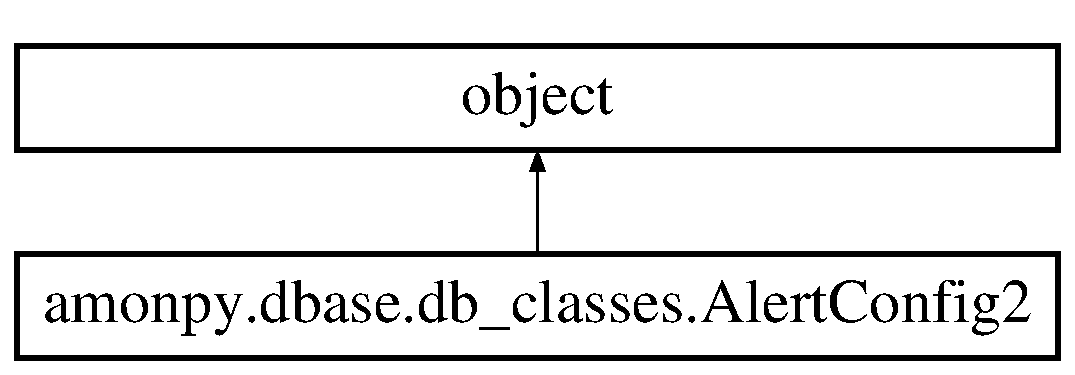
\includegraphics[height=2.000000cm]{df/d56/classamonpy_1_1dbase_1_1db__classes_1_1_alert_config2}
\end{center}
\end{figure}
\subsection*{Public Member Functions}
\begin{DoxyCompactItemize}
\item 
def \hyperlink{classamonpy_1_1dbase_1_1db__classes_1_1_alert_config2_af8f26a222e6993c3641895b85501a7dc}{\-\_\-\-\_\-init\-\_\-\-\_\-}
\item 
def \hyperlink{classamonpy_1_1dbase_1_1db__classes_1_1_alert_config2_ac28bc62a993c42b0e909f7cf7fdb6c50}{\-\_\-\-\_\-del\-\_\-\-\_\-}
\item 
def \hyperlink{classamonpy_1_1dbase_1_1db__classes_1_1_alert_config2_ae52dafae228b81cf695bcde9ddb724be}{forprint}
\end{DoxyCompactItemize}
\subsection*{Public Attributes}
\begin{DoxyCompactItemize}
\item 
\hyperlink{classamonpy_1_1dbase_1_1db__classes_1_1_alert_config2_a49f8af0cfc12e4f73da64323780102e8}{stream}
\item 
\hyperlink{classamonpy_1_1dbase_1_1db__classes_1_1_alert_config2_a44f00e5625906d6af0bda3a6f99f9c99}{rev}
\item 
\hyperlink{classamonpy_1_1dbase_1_1db__classes_1_1_alert_config2_a67a684e25c13f332b83baf748be6650d}{participating}
\item 
\hyperlink{classamonpy_1_1dbase_1_1db__classes_1_1_alert_config2_a8dbc3ae517192b47243d9cc10549c928}{p\-\_\-thresh}
\item 
\hyperlink{classamonpy_1_1dbase_1_1db__classes_1_1_alert_config2_aa4e9d2584bdecbd5b2c7be15784c7684}{N\-\_\-thresh}
\item 
\hyperlink{classamonpy_1_1dbase_1_1db__classes_1_1_alert_config2_ade495f929c328029a7a561b6a51e5914}{delta\-T}
\item 
\hyperlink{classamonpy_1_1dbase_1_1db__classes_1_1_alert_config2_a97fd6428426e51da12b281cf20dece5c}{buffer\-T}
\item 
\hyperlink{classamonpy_1_1dbase_1_1db__classes_1_1_alert_config2_a0467c2f3baa9c104d855b80898f8342f}{cluster\-\_\-method}
\item 
\hyperlink{classamonpy_1_1dbase_1_1db__classes_1_1_alert_config2_a32978aa8bf3558945e9e362ad55ed644}{cluster\-\_\-thresh}
\item 
\hyperlink{classamonpy_1_1dbase_1_1db__classes_1_1_alert_config2_acf76b84f2e496115285d95ccf2d60c22}{sens\-\_\-thresh}
\item 
\hyperlink{classamonpy_1_1dbase_1_1db__classes_1_1_alert_config2_af6d4d813406bf61fab7cd1d2de01766e}{psf\-\_\-param\-Desc1}
\item 
\hyperlink{classamonpy_1_1dbase_1_1db__classes_1_1_alert_config2_a8d604b6d92c7d6d1aa5d5a71e87c2f81}{psf\-\_\-param\-Desc2}
\item 
\hyperlink{classamonpy_1_1dbase_1_1db__classes_1_1_alert_config2_ab6fedbe0c3c5ddec221dd40f2118c3da}{psf\-\_\-param\-Desc3}
\item 
\hyperlink{classamonpy_1_1dbase_1_1db__classes_1_1_alert_config2_a3f204082c6db7abec1c48e3599a5fe0b}{skymap\-\_\-val1\-Desc}
\item 
\hyperlink{classamonpy_1_1dbase_1_1db__classes_1_1_alert_config2_ab819dfd55a24c72966efc393ecb82261}{skymap\-\_\-val2\-Desc}
\item 
\hyperlink{classamonpy_1_1dbase_1_1db__classes_1_1_alert_config2_a6c28894bd6690a2b0faeb36be8eb351f}{skymap\-\_\-val3\-Desc}
\item 
\hyperlink{classamonpy_1_1dbase_1_1db__classes_1_1_alert_config2_ac8bd043fc32dc2de20f5ee1cf57762e7}{valid\-Start}
\item 
\hyperlink{classamonpy_1_1dbase_1_1db__classes_1_1_alert_config2_a0338a9f4188da7e5b4e977a6d6a32dff}{valid\-Stop}
\item 
\hyperlink{classamonpy_1_1dbase_1_1db__classes_1_1_alert_config2_a94dabae815e574e6453b65d4efd9c0b0}{R\-\_\-thresh}
\end{DoxyCompactItemize}
\subsection*{Static Public Attributes}
\begin{DoxyCompactItemize}
\item 
int \hyperlink{classamonpy_1_1dbase_1_1db__classes_1_1_alert_config2_a17be669e8bdfa435ca0fe275a71479dd}{num\-\_\-configs} = 0
\end{DoxyCompactItemize}


\subsection{Detailed Description}
Creates the \hyperlink{classamonpy_1_1dbase_1_1db__classes_1_1_alert_config2}{Alert\-Config2} test class. 

Instances are created by specifying a unique double of I\-Ds (stream, rev). this version is used for testing the analysis code in Amon\-Py v0.\-1. Eventually, the two version will be unified into one. 

Definition at line 467 of file db\-\_\-classes.\-py.



\subsection{Constructor \& Destructor Documentation}
\hypertarget{classamonpy_1_1dbase_1_1db__classes_1_1_alert_config2_af8f26a222e6993c3641895b85501a7dc}{\index{amonpy\-::dbase\-::db\-\_\-classes\-::\-Alert\-Config2@{amonpy\-::dbase\-::db\-\_\-classes\-::\-Alert\-Config2}!\-\_\-\-\_\-init\-\_\-\-\_\-@{\-\_\-\-\_\-init\-\_\-\-\_\-}}
\index{\-\_\-\-\_\-init\-\_\-\-\_\-@{\-\_\-\-\_\-init\-\_\-\-\_\-}!amonpy::dbase::db_classes::AlertConfig2@{amonpy\-::dbase\-::db\-\_\-classes\-::\-Alert\-Config2}}
\subsubsection[{\-\_\-\-\_\-init\-\_\-\-\_\-}]{\setlength{\rightskip}{0pt plus 5cm}def amonpy.\-dbase.\-db\-\_\-classes.\-Alert\-Config2.\-\_\-\-\_\-init\-\_\-\-\_\- (
\begin{DoxyParamCaption}
\item[{}]{self, }
\item[{}]{stream, }
\item[{}]{rev}
\end{DoxyParamCaption}
)}}\label{classamonpy_1_1dbase_1_1db__classes_1_1_alert_config2_af8f26a222e6993c3641895b85501a7dc}


Definition at line 469 of file db\-\_\-classes.\-py.

\hypertarget{classamonpy_1_1dbase_1_1db__classes_1_1_alert_config2_ac28bc62a993c42b0e909f7cf7fdb6c50}{\index{amonpy\-::dbase\-::db\-\_\-classes\-::\-Alert\-Config2@{amonpy\-::dbase\-::db\-\_\-classes\-::\-Alert\-Config2}!\-\_\-\-\_\-del\-\_\-\-\_\-@{\-\_\-\-\_\-del\-\_\-\-\_\-}}
\index{\-\_\-\-\_\-del\-\_\-\-\_\-@{\-\_\-\-\_\-del\-\_\-\-\_\-}!amonpy::dbase::db_classes::AlertConfig2@{amonpy\-::dbase\-::db\-\_\-classes\-::\-Alert\-Config2}}
\subsubsection[{\-\_\-\-\_\-del\-\_\-\-\_\-}]{\setlength{\rightskip}{0pt plus 5cm}def amonpy.\-dbase.\-db\-\_\-classes.\-Alert\-Config2.\-\_\-\-\_\-del\-\_\-\-\_\- (
\begin{DoxyParamCaption}
\item[{}]{self}
\end{DoxyParamCaption}
)}}\label{classamonpy_1_1dbase_1_1db__classes_1_1_alert_config2_ac28bc62a993c42b0e909f7cf7fdb6c50}


Definition at line 491 of file db\-\_\-classes.\-py.



\subsection{Member Function Documentation}
\hypertarget{classamonpy_1_1dbase_1_1db__classes_1_1_alert_config2_ae52dafae228b81cf695bcde9ddb724be}{\index{amonpy\-::dbase\-::db\-\_\-classes\-::\-Alert\-Config2@{amonpy\-::dbase\-::db\-\_\-classes\-::\-Alert\-Config2}!forprint@{forprint}}
\index{forprint@{forprint}!amonpy::dbase::db_classes::AlertConfig2@{amonpy\-::dbase\-::db\-\_\-classes\-::\-Alert\-Config2}}
\subsubsection[{forprint}]{\setlength{\rightskip}{0pt plus 5cm}def amonpy.\-dbase.\-db\-\_\-classes.\-Alert\-Config2.\-forprint (
\begin{DoxyParamCaption}
\item[{}]{self}
\end{DoxyParamCaption}
)}}\label{classamonpy_1_1dbase_1_1db__classes_1_1_alert_config2_ae52dafae228b81cf695bcde9ddb724be}


Definition at line 494 of file db\-\_\-classes.\-py.



\subsection{Member Data Documentation}
\hypertarget{classamonpy_1_1dbase_1_1db__classes_1_1_alert_config2_a97fd6428426e51da12b281cf20dece5c}{\index{amonpy\-::dbase\-::db\-\_\-classes\-::\-Alert\-Config2@{amonpy\-::dbase\-::db\-\_\-classes\-::\-Alert\-Config2}!buffer\-T@{buffer\-T}}
\index{buffer\-T@{buffer\-T}!amonpy::dbase::db_classes::AlertConfig2@{amonpy\-::dbase\-::db\-\_\-classes\-::\-Alert\-Config2}}
\subsubsection[{buffer\-T}]{\setlength{\rightskip}{0pt plus 5cm}amonpy.\-dbase.\-db\-\_\-classes.\-Alert\-Config2.\-buffer\-T}}\label{classamonpy_1_1dbase_1_1db__classes_1_1_alert_config2_a97fd6428426e51da12b281cf20dece5c}


Definition at line 476 of file db\-\_\-classes.\-py.

\hypertarget{classamonpy_1_1dbase_1_1db__classes_1_1_alert_config2_a0467c2f3baa9c104d855b80898f8342f}{\index{amonpy\-::dbase\-::db\-\_\-classes\-::\-Alert\-Config2@{amonpy\-::dbase\-::db\-\_\-classes\-::\-Alert\-Config2}!cluster\-\_\-method@{cluster\-\_\-method}}
\index{cluster\-\_\-method@{cluster\-\_\-method}!amonpy::dbase::db_classes::AlertConfig2@{amonpy\-::dbase\-::db\-\_\-classes\-::\-Alert\-Config2}}
\subsubsection[{cluster\-\_\-method}]{\setlength{\rightskip}{0pt plus 5cm}amonpy.\-dbase.\-db\-\_\-classes.\-Alert\-Config2.\-cluster\-\_\-method}}\label{classamonpy_1_1dbase_1_1db__classes_1_1_alert_config2_a0467c2f3baa9c104d855b80898f8342f}


Definition at line 477 of file db\-\_\-classes.\-py.

\hypertarget{classamonpy_1_1dbase_1_1db__classes_1_1_alert_config2_a32978aa8bf3558945e9e362ad55ed644}{\index{amonpy\-::dbase\-::db\-\_\-classes\-::\-Alert\-Config2@{amonpy\-::dbase\-::db\-\_\-classes\-::\-Alert\-Config2}!cluster\-\_\-thresh@{cluster\-\_\-thresh}}
\index{cluster\-\_\-thresh@{cluster\-\_\-thresh}!amonpy::dbase::db_classes::AlertConfig2@{amonpy\-::dbase\-::db\-\_\-classes\-::\-Alert\-Config2}}
\subsubsection[{cluster\-\_\-thresh}]{\setlength{\rightskip}{0pt plus 5cm}amonpy.\-dbase.\-db\-\_\-classes.\-Alert\-Config2.\-cluster\-\_\-thresh}}\label{classamonpy_1_1dbase_1_1db__classes_1_1_alert_config2_a32978aa8bf3558945e9e362ad55ed644}


Definition at line 478 of file db\-\_\-classes.\-py.

\hypertarget{classamonpy_1_1dbase_1_1db__classes_1_1_alert_config2_ade495f929c328029a7a561b6a51e5914}{\index{amonpy\-::dbase\-::db\-\_\-classes\-::\-Alert\-Config2@{amonpy\-::dbase\-::db\-\_\-classes\-::\-Alert\-Config2}!delta\-T@{delta\-T}}
\index{delta\-T@{delta\-T}!amonpy::dbase::db_classes::AlertConfig2@{amonpy\-::dbase\-::db\-\_\-classes\-::\-Alert\-Config2}}
\subsubsection[{delta\-T}]{\setlength{\rightskip}{0pt plus 5cm}amonpy.\-dbase.\-db\-\_\-classes.\-Alert\-Config2.\-delta\-T}}\label{classamonpy_1_1dbase_1_1db__classes_1_1_alert_config2_ade495f929c328029a7a561b6a51e5914}


Definition at line 475 of file db\-\_\-classes.\-py.

\hypertarget{classamonpy_1_1dbase_1_1db__classes_1_1_alert_config2_aa4e9d2584bdecbd5b2c7be15784c7684}{\index{amonpy\-::dbase\-::db\-\_\-classes\-::\-Alert\-Config2@{amonpy\-::dbase\-::db\-\_\-classes\-::\-Alert\-Config2}!N\-\_\-thresh@{N\-\_\-thresh}}
\index{N\-\_\-thresh@{N\-\_\-thresh}!amonpy::dbase::db_classes::AlertConfig2@{amonpy\-::dbase\-::db\-\_\-classes\-::\-Alert\-Config2}}
\subsubsection[{N\-\_\-thresh}]{\setlength{\rightskip}{0pt plus 5cm}amonpy.\-dbase.\-db\-\_\-classes.\-Alert\-Config2.\-N\-\_\-thresh}}\label{classamonpy_1_1dbase_1_1db__classes_1_1_alert_config2_aa4e9d2584bdecbd5b2c7be15784c7684}


Definition at line 474 of file db\-\_\-classes.\-py.

\hypertarget{classamonpy_1_1dbase_1_1db__classes_1_1_alert_config2_a17be669e8bdfa435ca0fe275a71479dd}{\index{amonpy\-::dbase\-::db\-\_\-classes\-::\-Alert\-Config2@{amonpy\-::dbase\-::db\-\_\-classes\-::\-Alert\-Config2}!num\-\_\-configs@{num\-\_\-configs}}
\index{num\-\_\-configs@{num\-\_\-configs}!amonpy::dbase::db_classes::AlertConfig2@{amonpy\-::dbase\-::db\-\_\-classes\-::\-Alert\-Config2}}
\subsubsection[{num\-\_\-configs}]{\setlength{\rightskip}{0pt plus 5cm}int amonpy.\-dbase.\-db\-\_\-classes.\-Alert\-Config2.\-num\-\_\-configs = 0\hspace{0.3cm}{\ttfamily [static]}}}\label{classamonpy_1_1dbase_1_1db__classes_1_1_alert_config2_a17be669e8bdfa435ca0fe275a71479dd}


Definition at line 468 of file db\-\_\-classes.\-py.

\hypertarget{classamonpy_1_1dbase_1_1db__classes_1_1_alert_config2_a8dbc3ae517192b47243d9cc10549c928}{\index{amonpy\-::dbase\-::db\-\_\-classes\-::\-Alert\-Config2@{amonpy\-::dbase\-::db\-\_\-classes\-::\-Alert\-Config2}!p\-\_\-thresh@{p\-\_\-thresh}}
\index{p\-\_\-thresh@{p\-\_\-thresh}!amonpy::dbase::db_classes::AlertConfig2@{amonpy\-::dbase\-::db\-\_\-classes\-::\-Alert\-Config2}}
\subsubsection[{p\-\_\-thresh}]{\setlength{\rightskip}{0pt plus 5cm}amonpy.\-dbase.\-db\-\_\-classes.\-Alert\-Config2.\-p\-\_\-thresh}}\label{classamonpy_1_1dbase_1_1db__classes_1_1_alert_config2_a8dbc3ae517192b47243d9cc10549c928}


Definition at line 473 of file db\-\_\-classes.\-py.

\hypertarget{classamonpy_1_1dbase_1_1db__classes_1_1_alert_config2_a67a684e25c13f332b83baf748be6650d}{\index{amonpy\-::dbase\-::db\-\_\-classes\-::\-Alert\-Config2@{amonpy\-::dbase\-::db\-\_\-classes\-::\-Alert\-Config2}!participating@{participating}}
\index{participating@{participating}!amonpy::dbase::db_classes::AlertConfig2@{amonpy\-::dbase\-::db\-\_\-classes\-::\-Alert\-Config2}}
\subsubsection[{participating}]{\setlength{\rightskip}{0pt plus 5cm}amonpy.\-dbase.\-db\-\_\-classes.\-Alert\-Config2.\-participating}}\label{classamonpy_1_1dbase_1_1db__classes_1_1_alert_config2_a67a684e25c13f332b83baf748be6650d}


Definition at line 472 of file db\-\_\-classes.\-py.

\hypertarget{classamonpy_1_1dbase_1_1db__classes_1_1_alert_config2_af6d4d813406bf61fab7cd1d2de01766e}{\index{amonpy\-::dbase\-::db\-\_\-classes\-::\-Alert\-Config2@{amonpy\-::dbase\-::db\-\_\-classes\-::\-Alert\-Config2}!psf\-\_\-param\-Desc1@{psf\-\_\-param\-Desc1}}
\index{psf\-\_\-param\-Desc1@{psf\-\_\-param\-Desc1}!amonpy::dbase::db_classes::AlertConfig2@{amonpy\-::dbase\-::db\-\_\-classes\-::\-Alert\-Config2}}
\subsubsection[{psf\-\_\-param\-Desc1}]{\setlength{\rightskip}{0pt plus 5cm}amonpy.\-dbase.\-db\-\_\-classes.\-Alert\-Config2.\-psf\-\_\-param\-Desc1}}\label{classamonpy_1_1dbase_1_1db__classes_1_1_alert_config2_af6d4d813406bf61fab7cd1d2de01766e}


Definition at line 480 of file db\-\_\-classes.\-py.

\hypertarget{classamonpy_1_1dbase_1_1db__classes_1_1_alert_config2_a8d604b6d92c7d6d1aa5d5a71e87c2f81}{\index{amonpy\-::dbase\-::db\-\_\-classes\-::\-Alert\-Config2@{amonpy\-::dbase\-::db\-\_\-classes\-::\-Alert\-Config2}!psf\-\_\-param\-Desc2@{psf\-\_\-param\-Desc2}}
\index{psf\-\_\-param\-Desc2@{psf\-\_\-param\-Desc2}!amonpy::dbase::db_classes::AlertConfig2@{amonpy\-::dbase\-::db\-\_\-classes\-::\-Alert\-Config2}}
\subsubsection[{psf\-\_\-param\-Desc2}]{\setlength{\rightskip}{0pt plus 5cm}amonpy.\-dbase.\-db\-\_\-classes.\-Alert\-Config2.\-psf\-\_\-param\-Desc2}}\label{classamonpy_1_1dbase_1_1db__classes_1_1_alert_config2_a8d604b6d92c7d6d1aa5d5a71e87c2f81}


Definition at line 481 of file db\-\_\-classes.\-py.

\hypertarget{classamonpy_1_1dbase_1_1db__classes_1_1_alert_config2_ab6fedbe0c3c5ddec221dd40f2118c3da}{\index{amonpy\-::dbase\-::db\-\_\-classes\-::\-Alert\-Config2@{amonpy\-::dbase\-::db\-\_\-classes\-::\-Alert\-Config2}!psf\-\_\-param\-Desc3@{psf\-\_\-param\-Desc3}}
\index{psf\-\_\-param\-Desc3@{psf\-\_\-param\-Desc3}!amonpy::dbase::db_classes::AlertConfig2@{amonpy\-::dbase\-::db\-\_\-classes\-::\-Alert\-Config2}}
\subsubsection[{psf\-\_\-param\-Desc3}]{\setlength{\rightskip}{0pt plus 5cm}amonpy.\-dbase.\-db\-\_\-classes.\-Alert\-Config2.\-psf\-\_\-param\-Desc3}}\label{classamonpy_1_1dbase_1_1db__classes_1_1_alert_config2_ab6fedbe0c3c5ddec221dd40f2118c3da}


Definition at line 482 of file db\-\_\-classes.\-py.

\hypertarget{classamonpy_1_1dbase_1_1db__classes_1_1_alert_config2_a94dabae815e574e6453b65d4efd9c0b0}{\index{amonpy\-::dbase\-::db\-\_\-classes\-::\-Alert\-Config2@{amonpy\-::dbase\-::db\-\_\-classes\-::\-Alert\-Config2}!R\-\_\-thresh@{R\-\_\-thresh}}
\index{R\-\_\-thresh@{R\-\_\-thresh}!amonpy::dbase::db_classes::AlertConfig2@{amonpy\-::dbase\-::db\-\_\-classes\-::\-Alert\-Config2}}
\subsubsection[{R\-\_\-thresh}]{\setlength{\rightskip}{0pt plus 5cm}amonpy.\-dbase.\-db\-\_\-classes.\-Alert\-Config2.\-R\-\_\-thresh}}\label{classamonpy_1_1dbase_1_1db__classes_1_1_alert_config2_a94dabae815e574e6453b65d4efd9c0b0}


Definition at line 488 of file db\-\_\-classes.\-py.

\hypertarget{classamonpy_1_1dbase_1_1db__classes_1_1_alert_config2_a44f00e5625906d6af0bda3a6f99f9c99}{\index{amonpy\-::dbase\-::db\-\_\-classes\-::\-Alert\-Config2@{amonpy\-::dbase\-::db\-\_\-classes\-::\-Alert\-Config2}!rev@{rev}}
\index{rev@{rev}!amonpy::dbase::db_classes::AlertConfig2@{amonpy\-::dbase\-::db\-\_\-classes\-::\-Alert\-Config2}}
\subsubsection[{rev}]{\setlength{\rightskip}{0pt plus 5cm}amonpy.\-dbase.\-db\-\_\-classes.\-Alert\-Config2.\-rev}}\label{classamonpy_1_1dbase_1_1db__classes_1_1_alert_config2_a44f00e5625906d6af0bda3a6f99f9c99}


Definition at line 471 of file db\-\_\-classes.\-py.

\hypertarget{classamonpy_1_1dbase_1_1db__classes_1_1_alert_config2_acf76b84f2e496115285d95ccf2d60c22}{\index{amonpy\-::dbase\-::db\-\_\-classes\-::\-Alert\-Config2@{amonpy\-::dbase\-::db\-\_\-classes\-::\-Alert\-Config2}!sens\-\_\-thresh@{sens\-\_\-thresh}}
\index{sens\-\_\-thresh@{sens\-\_\-thresh}!amonpy::dbase::db_classes::AlertConfig2@{amonpy\-::dbase\-::db\-\_\-classes\-::\-Alert\-Config2}}
\subsubsection[{sens\-\_\-thresh}]{\setlength{\rightskip}{0pt plus 5cm}amonpy.\-dbase.\-db\-\_\-classes.\-Alert\-Config2.\-sens\-\_\-thresh}}\label{classamonpy_1_1dbase_1_1db__classes_1_1_alert_config2_acf76b84f2e496115285d95ccf2d60c22}


Definition at line 479 of file db\-\_\-classes.\-py.

\hypertarget{classamonpy_1_1dbase_1_1db__classes_1_1_alert_config2_a3f204082c6db7abec1c48e3599a5fe0b}{\index{amonpy\-::dbase\-::db\-\_\-classes\-::\-Alert\-Config2@{amonpy\-::dbase\-::db\-\_\-classes\-::\-Alert\-Config2}!skymap\-\_\-val1\-Desc@{skymap\-\_\-val1\-Desc}}
\index{skymap\-\_\-val1\-Desc@{skymap\-\_\-val1\-Desc}!amonpy::dbase::db_classes::AlertConfig2@{amonpy\-::dbase\-::db\-\_\-classes\-::\-Alert\-Config2}}
\subsubsection[{skymap\-\_\-val1\-Desc}]{\setlength{\rightskip}{0pt plus 5cm}amonpy.\-dbase.\-db\-\_\-classes.\-Alert\-Config2.\-skymap\-\_\-val1\-Desc}}\label{classamonpy_1_1dbase_1_1db__classes_1_1_alert_config2_a3f204082c6db7abec1c48e3599a5fe0b}


Definition at line 483 of file db\-\_\-classes.\-py.

\hypertarget{classamonpy_1_1dbase_1_1db__classes_1_1_alert_config2_ab819dfd55a24c72966efc393ecb82261}{\index{amonpy\-::dbase\-::db\-\_\-classes\-::\-Alert\-Config2@{amonpy\-::dbase\-::db\-\_\-classes\-::\-Alert\-Config2}!skymap\-\_\-val2\-Desc@{skymap\-\_\-val2\-Desc}}
\index{skymap\-\_\-val2\-Desc@{skymap\-\_\-val2\-Desc}!amonpy::dbase::db_classes::AlertConfig2@{amonpy\-::dbase\-::db\-\_\-classes\-::\-Alert\-Config2}}
\subsubsection[{skymap\-\_\-val2\-Desc}]{\setlength{\rightskip}{0pt plus 5cm}amonpy.\-dbase.\-db\-\_\-classes.\-Alert\-Config2.\-skymap\-\_\-val2\-Desc}}\label{classamonpy_1_1dbase_1_1db__classes_1_1_alert_config2_ab819dfd55a24c72966efc393ecb82261}


Definition at line 484 of file db\-\_\-classes.\-py.

\hypertarget{classamonpy_1_1dbase_1_1db__classes_1_1_alert_config2_a6c28894bd6690a2b0faeb36be8eb351f}{\index{amonpy\-::dbase\-::db\-\_\-classes\-::\-Alert\-Config2@{amonpy\-::dbase\-::db\-\_\-classes\-::\-Alert\-Config2}!skymap\-\_\-val3\-Desc@{skymap\-\_\-val3\-Desc}}
\index{skymap\-\_\-val3\-Desc@{skymap\-\_\-val3\-Desc}!amonpy::dbase::db_classes::AlertConfig2@{amonpy\-::dbase\-::db\-\_\-classes\-::\-Alert\-Config2}}
\subsubsection[{skymap\-\_\-val3\-Desc}]{\setlength{\rightskip}{0pt plus 5cm}amonpy.\-dbase.\-db\-\_\-classes.\-Alert\-Config2.\-skymap\-\_\-val3\-Desc}}\label{classamonpy_1_1dbase_1_1db__classes_1_1_alert_config2_a6c28894bd6690a2b0faeb36be8eb351f}


Definition at line 485 of file db\-\_\-classes.\-py.

\hypertarget{classamonpy_1_1dbase_1_1db__classes_1_1_alert_config2_a49f8af0cfc12e4f73da64323780102e8}{\index{amonpy\-::dbase\-::db\-\_\-classes\-::\-Alert\-Config2@{amonpy\-::dbase\-::db\-\_\-classes\-::\-Alert\-Config2}!stream@{stream}}
\index{stream@{stream}!amonpy::dbase::db_classes::AlertConfig2@{amonpy\-::dbase\-::db\-\_\-classes\-::\-Alert\-Config2}}
\subsubsection[{stream}]{\setlength{\rightskip}{0pt plus 5cm}amonpy.\-dbase.\-db\-\_\-classes.\-Alert\-Config2.\-stream}}\label{classamonpy_1_1dbase_1_1db__classes_1_1_alert_config2_a49f8af0cfc12e4f73da64323780102e8}


Definition at line 470 of file db\-\_\-classes.\-py.

\hypertarget{classamonpy_1_1dbase_1_1db__classes_1_1_alert_config2_ac8bd043fc32dc2de20f5ee1cf57762e7}{\index{amonpy\-::dbase\-::db\-\_\-classes\-::\-Alert\-Config2@{amonpy\-::dbase\-::db\-\_\-classes\-::\-Alert\-Config2}!valid\-Start@{valid\-Start}}
\index{valid\-Start@{valid\-Start}!amonpy::dbase::db_classes::AlertConfig2@{amonpy\-::dbase\-::db\-\_\-classes\-::\-Alert\-Config2}}
\subsubsection[{valid\-Start}]{\setlength{\rightskip}{0pt plus 5cm}amonpy.\-dbase.\-db\-\_\-classes.\-Alert\-Config2.\-valid\-Start}}\label{classamonpy_1_1dbase_1_1db__classes_1_1_alert_config2_ac8bd043fc32dc2de20f5ee1cf57762e7}


Definition at line 486 of file db\-\_\-classes.\-py.

\hypertarget{classamonpy_1_1dbase_1_1db__classes_1_1_alert_config2_a0338a9f4188da7e5b4e977a6d6a32dff}{\index{amonpy\-::dbase\-::db\-\_\-classes\-::\-Alert\-Config2@{amonpy\-::dbase\-::db\-\_\-classes\-::\-Alert\-Config2}!valid\-Stop@{valid\-Stop}}
\index{valid\-Stop@{valid\-Stop}!amonpy::dbase::db_classes::AlertConfig2@{amonpy\-::dbase\-::db\-\_\-classes\-::\-Alert\-Config2}}
\subsubsection[{valid\-Stop}]{\setlength{\rightskip}{0pt plus 5cm}amonpy.\-dbase.\-db\-\_\-classes.\-Alert\-Config2.\-valid\-Stop}}\label{classamonpy_1_1dbase_1_1db__classes_1_1_alert_config2_a0338a9f4188da7e5b4e977a6d6a32dff}


Definition at line 487 of file db\-\_\-classes.\-py.



The documentation for this class was generated from the following file\-:\begin{DoxyCompactItemize}
\item 
amonpy/dbase/\hyperlink{db__classes_8py}{db\-\_\-classes.\-py}\end{DoxyCompactItemize}

\hypertarget{classamonpy_1_1dbase_1_1db__classes_1_1_alert_line}{\section{amonpy.\-dbase.\-db\-\_\-classes.\-Alert\-Line Class Reference}
\label{classamonpy_1_1dbase_1_1db__classes_1_1_alert_line}\index{amonpy.\-dbase.\-db\-\_\-classes.\-Alert\-Line@{amonpy.\-dbase.\-db\-\_\-classes.\-Alert\-Line}}
}


Creates the \hyperlink{classamonpy_1_1dbase_1_1db__classes_1_1_alert_line}{Alert\-Line} class.  


Inheritance diagram for amonpy.\-dbase.\-db\-\_\-classes.\-Alert\-Line\-:\begin{figure}[H]
\begin{center}
\leavevmode
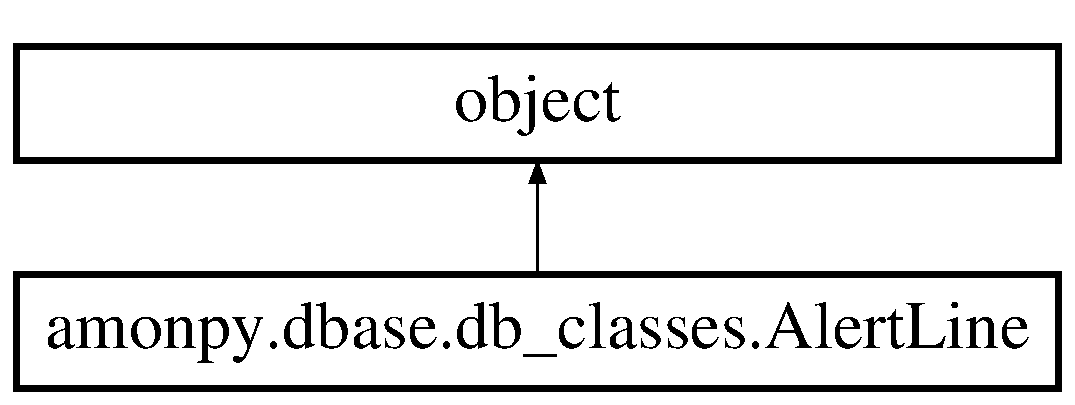
\includegraphics[height=2.000000cm]{d5/d8e/classamonpy_1_1dbase_1_1db__classes_1_1_alert_line}
\end{center}
\end{figure}
\subsection*{Public Member Functions}
\begin{DoxyCompactItemize}
\item 
def \hyperlink{classamonpy_1_1dbase_1_1db__classes_1_1_alert_line_aef4fa3d64975b679df843c3b1cbcfb8e}{\-\_\-\-\_\-init\-\_\-\-\_\-}
\item 
def \hyperlink{classamonpy_1_1dbase_1_1db__classes_1_1_alert_line_a835e26d237c6fa3c78cddc18b2b8d9ff}{\-\_\-\-\_\-del\-\_\-\-\_\-}
\item 
def \hyperlink{classamonpy_1_1dbase_1_1db__classes_1_1_alert_line_a3ab6ec496d54160c4069f47237776646}{forprint}
\end{DoxyCompactItemize}
\subsection*{Public Attributes}
\begin{DoxyCompactItemize}
\item 
\hyperlink{classamonpy_1_1dbase_1_1db__classes_1_1_alert_line_ab24de2d5e3f4418dc2b9c6c68c42ae41}{stream\-\_\-alert}
\item 
\hyperlink{classamonpy_1_1dbase_1_1db__classes_1_1_alert_line_afe155f528e6c01f810d95264e77ccee6}{id\-\_\-alert}
\item 
\hyperlink{classamonpy_1_1dbase_1_1db__classes_1_1_alert_line_acb48088679522c813ac7ad21924f98a1}{rev\-\_\-alert}
\item 
\hyperlink{classamonpy_1_1dbase_1_1db__classes_1_1_alert_line_a6081f9c41c7c34d54a565407f2308175}{stream\-\_\-event}
\item 
\hyperlink{classamonpy_1_1dbase_1_1db__classes_1_1_alert_line_abbf3c5c8916d6a655444f44a841705f7}{id\-\_\-event}
\item 
\hyperlink{classamonpy_1_1dbase_1_1db__classes_1_1_alert_line_a5180b21c821a1eb9540d88623e11378f}{rev\-\_\-event}
\end{DoxyCompactItemize}
\subsection*{Static Public Attributes}
\begin{DoxyCompactItemize}
\item 
int \hyperlink{classamonpy_1_1dbase_1_1db__classes_1_1_alert_line_a8450803058ff3da20dc1a9001b77082f}{num\-\_\-alertlines} = 0
\end{DoxyCompactItemize}


\subsection{Detailed Description}
Creates the \hyperlink{classamonpy_1_1dbase_1_1db__classes_1_1_alert_line}{Alert\-Line} class. 

Instances created by specifying a unique 6 I\-Ds (stream\-\_\-alert, id\-\_\-alert, rev\-\_\-alert, stream\-\_\-event, id\-\_\-event, rev\-\_\-event) 

Definition at line 535 of file db\-\_\-classes.\-py.



\subsection{Constructor \& Destructor Documentation}
\hypertarget{classamonpy_1_1dbase_1_1db__classes_1_1_alert_line_aef4fa3d64975b679df843c3b1cbcfb8e}{\index{amonpy\-::dbase\-::db\-\_\-classes\-::\-Alert\-Line@{amonpy\-::dbase\-::db\-\_\-classes\-::\-Alert\-Line}!\-\_\-\-\_\-init\-\_\-\-\_\-@{\-\_\-\-\_\-init\-\_\-\-\_\-}}
\index{\-\_\-\-\_\-init\-\_\-\-\_\-@{\-\_\-\-\_\-init\-\_\-\-\_\-}!amonpy::dbase::db_classes::AlertLine@{amonpy\-::dbase\-::db\-\_\-classes\-::\-Alert\-Line}}
\subsubsection[{\-\_\-\-\_\-init\-\_\-\-\_\-}]{\setlength{\rightskip}{0pt plus 5cm}def amonpy.\-dbase.\-db\-\_\-classes.\-Alert\-Line.\-\_\-\-\_\-init\-\_\-\-\_\- (
\begin{DoxyParamCaption}
\item[{}]{self, }
\item[{}]{astream, }
\item[{}]{aid, }
\item[{}]{arev, }
\item[{}]{estream, }
\item[{}]{eid, }
\item[{}]{erev}
\end{DoxyParamCaption}
)}}\label{classamonpy_1_1dbase_1_1db__classes_1_1_alert_line_aef4fa3d64975b679df843c3b1cbcfb8e}


Definition at line 537 of file db\-\_\-classes.\-py.

\hypertarget{classamonpy_1_1dbase_1_1db__classes_1_1_alert_line_a835e26d237c6fa3c78cddc18b2b8d9ff}{\index{amonpy\-::dbase\-::db\-\_\-classes\-::\-Alert\-Line@{amonpy\-::dbase\-::db\-\_\-classes\-::\-Alert\-Line}!\-\_\-\-\_\-del\-\_\-\-\_\-@{\-\_\-\-\_\-del\-\_\-\-\_\-}}
\index{\-\_\-\-\_\-del\-\_\-\-\_\-@{\-\_\-\-\_\-del\-\_\-\-\_\-}!amonpy::dbase::db_classes::AlertLine@{amonpy\-::dbase\-::db\-\_\-classes\-::\-Alert\-Line}}
\subsubsection[{\-\_\-\-\_\-del\-\_\-\-\_\-}]{\setlength{\rightskip}{0pt plus 5cm}def amonpy.\-dbase.\-db\-\_\-classes.\-Alert\-Line.\-\_\-\-\_\-del\-\_\-\-\_\- (
\begin{DoxyParamCaption}
\item[{}]{self}
\end{DoxyParamCaption}
)}}\label{classamonpy_1_1dbase_1_1db__classes_1_1_alert_line_a835e26d237c6fa3c78cddc18b2b8d9ff}


Definition at line 546 of file db\-\_\-classes.\-py.



\subsection{Member Function Documentation}
\hypertarget{classamonpy_1_1dbase_1_1db__classes_1_1_alert_line_a3ab6ec496d54160c4069f47237776646}{\index{amonpy\-::dbase\-::db\-\_\-classes\-::\-Alert\-Line@{amonpy\-::dbase\-::db\-\_\-classes\-::\-Alert\-Line}!forprint@{forprint}}
\index{forprint@{forprint}!amonpy::dbase::db_classes::AlertLine@{amonpy\-::dbase\-::db\-\_\-classes\-::\-Alert\-Line}}
\subsubsection[{forprint}]{\setlength{\rightskip}{0pt plus 5cm}def amonpy.\-dbase.\-db\-\_\-classes.\-Alert\-Line.\-forprint (
\begin{DoxyParamCaption}
\item[{}]{self}
\end{DoxyParamCaption}
)}}\label{classamonpy_1_1dbase_1_1db__classes_1_1_alert_line_a3ab6ec496d54160c4069f47237776646}


Definition at line 549 of file db\-\_\-classes.\-py.



\subsection{Member Data Documentation}
\hypertarget{classamonpy_1_1dbase_1_1db__classes_1_1_alert_line_afe155f528e6c01f810d95264e77ccee6}{\index{amonpy\-::dbase\-::db\-\_\-classes\-::\-Alert\-Line@{amonpy\-::dbase\-::db\-\_\-classes\-::\-Alert\-Line}!id\-\_\-alert@{id\-\_\-alert}}
\index{id\-\_\-alert@{id\-\_\-alert}!amonpy::dbase::db_classes::AlertLine@{amonpy\-::dbase\-::db\-\_\-classes\-::\-Alert\-Line}}
\subsubsection[{id\-\_\-alert}]{\setlength{\rightskip}{0pt plus 5cm}amonpy.\-dbase.\-db\-\_\-classes.\-Alert\-Line.\-id\-\_\-alert}}\label{classamonpy_1_1dbase_1_1db__classes_1_1_alert_line_afe155f528e6c01f810d95264e77ccee6}


Definition at line 539 of file db\-\_\-classes.\-py.

\hypertarget{classamonpy_1_1dbase_1_1db__classes_1_1_alert_line_abbf3c5c8916d6a655444f44a841705f7}{\index{amonpy\-::dbase\-::db\-\_\-classes\-::\-Alert\-Line@{amonpy\-::dbase\-::db\-\_\-classes\-::\-Alert\-Line}!id\-\_\-event@{id\-\_\-event}}
\index{id\-\_\-event@{id\-\_\-event}!amonpy::dbase::db_classes::AlertLine@{amonpy\-::dbase\-::db\-\_\-classes\-::\-Alert\-Line}}
\subsubsection[{id\-\_\-event}]{\setlength{\rightskip}{0pt plus 5cm}amonpy.\-dbase.\-db\-\_\-classes.\-Alert\-Line.\-id\-\_\-event}}\label{classamonpy_1_1dbase_1_1db__classes_1_1_alert_line_abbf3c5c8916d6a655444f44a841705f7}


Definition at line 542 of file db\-\_\-classes.\-py.

\hypertarget{classamonpy_1_1dbase_1_1db__classes_1_1_alert_line_a8450803058ff3da20dc1a9001b77082f}{\index{amonpy\-::dbase\-::db\-\_\-classes\-::\-Alert\-Line@{amonpy\-::dbase\-::db\-\_\-classes\-::\-Alert\-Line}!num\-\_\-alertlines@{num\-\_\-alertlines}}
\index{num\-\_\-alertlines@{num\-\_\-alertlines}!amonpy::dbase::db_classes::AlertLine@{amonpy\-::dbase\-::db\-\_\-classes\-::\-Alert\-Line}}
\subsubsection[{num\-\_\-alertlines}]{\setlength{\rightskip}{0pt plus 5cm}int amonpy.\-dbase.\-db\-\_\-classes.\-Alert\-Line.\-num\-\_\-alertlines = 0\hspace{0.3cm}{\ttfamily [static]}}}\label{classamonpy_1_1dbase_1_1db__classes_1_1_alert_line_a8450803058ff3da20dc1a9001b77082f}


Definition at line 536 of file db\-\_\-classes.\-py.

\hypertarget{classamonpy_1_1dbase_1_1db__classes_1_1_alert_line_acb48088679522c813ac7ad21924f98a1}{\index{amonpy\-::dbase\-::db\-\_\-classes\-::\-Alert\-Line@{amonpy\-::dbase\-::db\-\_\-classes\-::\-Alert\-Line}!rev\-\_\-alert@{rev\-\_\-alert}}
\index{rev\-\_\-alert@{rev\-\_\-alert}!amonpy::dbase::db_classes::AlertLine@{amonpy\-::dbase\-::db\-\_\-classes\-::\-Alert\-Line}}
\subsubsection[{rev\-\_\-alert}]{\setlength{\rightskip}{0pt plus 5cm}amonpy.\-dbase.\-db\-\_\-classes.\-Alert\-Line.\-rev\-\_\-alert}}\label{classamonpy_1_1dbase_1_1db__classes_1_1_alert_line_acb48088679522c813ac7ad21924f98a1}


Definition at line 540 of file db\-\_\-classes.\-py.

\hypertarget{classamonpy_1_1dbase_1_1db__classes_1_1_alert_line_a5180b21c821a1eb9540d88623e11378f}{\index{amonpy\-::dbase\-::db\-\_\-classes\-::\-Alert\-Line@{amonpy\-::dbase\-::db\-\_\-classes\-::\-Alert\-Line}!rev\-\_\-event@{rev\-\_\-event}}
\index{rev\-\_\-event@{rev\-\_\-event}!amonpy::dbase::db_classes::AlertLine@{amonpy\-::dbase\-::db\-\_\-classes\-::\-Alert\-Line}}
\subsubsection[{rev\-\_\-event}]{\setlength{\rightskip}{0pt plus 5cm}amonpy.\-dbase.\-db\-\_\-classes.\-Alert\-Line.\-rev\-\_\-event}}\label{classamonpy_1_1dbase_1_1db__classes_1_1_alert_line_a5180b21c821a1eb9540d88623e11378f}


Definition at line 543 of file db\-\_\-classes.\-py.

\hypertarget{classamonpy_1_1dbase_1_1db__classes_1_1_alert_line_ab24de2d5e3f4418dc2b9c6c68c42ae41}{\index{amonpy\-::dbase\-::db\-\_\-classes\-::\-Alert\-Line@{amonpy\-::dbase\-::db\-\_\-classes\-::\-Alert\-Line}!stream\-\_\-alert@{stream\-\_\-alert}}
\index{stream\-\_\-alert@{stream\-\_\-alert}!amonpy::dbase::db_classes::AlertLine@{amonpy\-::dbase\-::db\-\_\-classes\-::\-Alert\-Line}}
\subsubsection[{stream\-\_\-alert}]{\setlength{\rightskip}{0pt plus 5cm}amonpy.\-dbase.\-db\-\_\-classes.\-Alert\-Line.\-stream\-\_\-alert}}\label{classamonpy_1_1dbase_1_1db__classes_1_1_alert_line_ab24de2d5e3f4418dc2b9c6c68c42ae41}


Definition at line 538 of file db\-\_\-classes.\-py.

\hypertarget{classamonpy_1_1dbase_1_1db__classes_1_1_alert_line_a6081f9c41c7c34d54a565407f2308175}{\index{amonpy\-::dbase\-::db\-\_\-classes\-::\-Alert\-Line@{amonpy\-::dbase\-::db\-\_\-classes\-::\-Alert\-Line}!stream\-\_\-event@{stream\-\_\-event}}
\index{stream\-\_\-event@{stream\-\_\-event}!amonpy::dbase::db_classes::AlertLine@{amonpy\-::dbase\-::db\-\_\-classes\-::\-Alert\-Line}}
\subsubsection[{stream\-\_\-event}]{\setlength{\rightskip}{0pt plus 5cm}amonpy.\-dbase.\-db\-\_\-classes.\-Alert\-Line.\-stream\-\_\-event}}\label{classamonpy_1_1dbase_1_1db__classes_1_1_alert_line_a6081f9c41c7c34d54a565407f2308175}


Definition at line 541 of file db\-\_\-classes.\-py.



The documentation for this class was generated from the following file\-:\begin{DoxyCompactItemize}
\item 
amonpy/dbase/\hyperlink{db__classes_8py}{db\-\_\-classes.\-py}\end{DoxyCompactItemize}

\hypertarget{classamonpy_1_1sim_1_1sidereal_1_1_alt_az}{\section{amonpy.\-sim.\-sidereal.\-Alt\-Az Class Reference}
\label{classamonpy_1_1sim_1_1sidereal_1_1_alt_az}\index{amonpy.\-sim.\-sidereal.\-Alt\-Az@{amonpy.\-sim.\-sidereal.\-Alt\-Az}}
}


Represents a sky location in horizon coords.  




\subsection{Detailed Description}
Represents a sky location in horizon coords. 

(altitude/azimuth) \begin{DoxyVerb}  Exports/Invariants:
    .alt:   [ altitude in radians, in [-pi,+pi] ]
    .az:    [ azimuth in radians, in [0,2*pi] ]\end{DoxyVerb}
 

Definition at line 1368 of file sidereal.\-py.



The documentation for this class was generated from the following file\-:\begin{DoxyCompactItemize}
\item 
amonpy/sim/\hyperlink{sidereal_8py}{sidereal.\-py}\end{DoxyCompactItemize}

\hypertarget{classamonpy_1_1sim_1_1sidereal__m_1_1_alt_az}{\section{amonpy.\-sim.\-sidereal\-\_\-m.\-Alt\-Az Class Reference}
\label{classamonpy_1_1sim_1_1sidereal__m_1_1_alt_az}\index{amonpy.\-sim.\-sidereal\-\_\-m.\-Alt\-Az@{amonpy.\-sim.\-sidereal\-\_\-m.\-Alt\-Az}}
}
\subsection*{Public Member Functions}
\begin{DoxyCompactItemize}
\item 
def \hyperlink{classamonpy_1_1sim_1_1sidereal__m_1_1_alt_az_a67a6214cfaf80bbc6430f369cdb63a2b}{\-\_\-\-\_\-init\-\_\-\-\_\-}
\item 
def \hyperlink{classamonpy_1_1sim_1_1sidereal__m_1_1_alt_az_a5c119d0011e0e44ac11e924f21dc652d}{ra\-Dec}
\item 
def \hyperlink{classamonpy_1_1sim_1_1sidereal__m_1_1_alt_az_a40aadadac18ad5011e8818dc82b23e4c}{\-\_\-\-\_\-str\-\_\-\-\_\-}
\end{DoxyCompactItemize}
\subsection*{Public Attributes}
\begin{DoxyCompactItemize}
\item 
\hyperlink{classamonpy_1_1sim_1_1sidereal__m_1_1_alt_az_aa0ff247b310a833a5391c0b09f939d3b}{alt}
\item 
\hyperlink{classamonpy_1_1sim_1_1sidereal__m_1_1_alt_az_ab076f42a7d43bb00902e111c345e43c0}{az}
\end{DoxyCompactItemize}


\subsection{Detailed Description}
\begin{DoxyVerb}Represents a sky location in horizon coords. (altitude/azimuth)

  Exports/Invariants:
    .alt:   [ altitude in radians, in [-pi,+pi] ]
    .az:    [ azimuth in radians, in [0,2*pi] ]
\end{DoxyVerb}
 

\subsection{Constructor \& Destructor Documentation}
\hypertarget{classamonpy_1_1sim_1_1sidereal__m_1_1_alt_az_a67a6214cfaf80bbc6430f369cdb63a2b}{\index{amonpy\-::sim\-::sidereal\-\_\-m\-::\-Alt\-Az@{amonpy\-::sim\-::sidereal\-\_\-m\-::\-Alt\-Az}!\-\_\-\-\_\-init\-\_\-\-\_\-@{\-\_\-\-\_\-init\-\_\-\-\_\-}}
\index{\-\_\-\-\_\-init\-\_\-\-\_\-@{\-\_\-\-\_\-init\-\_\-\-\_\-}!amonpy::sim::sidereal_m::AltAz@{amonpy\-::sim\-::sidereal\-\_\-m\-::\-Alt\-Az}}
\subsubsection[{\-\_\-\-\_\-init\-\_\-\-\_\-}]{\setlength{\rightskip}{0pt plus 5cm}def amonpy.\-sim.\-sidereal\-\_\-m.\-Alt\-Az.\-\_\-\-\_\-init\-\_\-\-\_\- (
\begin{DoxyParamCaption}
\item[{}]{self, }
\item[{}]{alt, }
\item[{}]{az}
\end{DoxyParamCaption}
)}}\label{classamonpy_1_1sim_1_1sidereal__m_1_1_alt_az_a67a6214cfaf80bbc6430f369cdb63a2b}
\begin{DoxyVerb}Constructor for AltAz, horizon coordinates.

  [ (alt is an altitude in radians) and
    (az is an azimuth in radians) ->
      return a new AltAz instance with those values,
      normalized as per class invariants ]
\end{DoxyVerb}
 

\subsection{Member Function Documentation}
\hypertarget{classamonpy_1_1sim_1_1sidereal__m_1_1_alt_az_a40aadadac18ad5011e8818dc82b23e4c}{\index{amonpy\-::sim\-::sidereal\-\_\-m\-::\-Alt\-Az@{amonpy\-::sim\-::sidereal\-\_\-m\-::\-Alt\-Az}!\-\_\-\-\_\-str\-\_\-\-\_\-@{\-\_\-\-\_\-str\-\_\-\-\_\-}}
\index{\-\_\-\-\_\-str\-\_\-\-\_\-@{\-\_\-\-\_\-str\-\_\-\-\_\-}!amonpy::sim::sidereal_m::AltAz@{amonpy\-::sim\-::sidereal\-\_\-m\-::\-Alt\-Az}}
\subsubsection[{\-\_\-\-\_\-str\-\_\-\-\_\-}]{\setlength{\rightskip}{0pt plus 5cm}def amonpy.\-sim.\-sidereal\-\_\-m.\-Alt\-Az.\-\_\-\-\_\-str\-\_\-\-\_\- (
\begin{DoxyParamCaption}
\item[{}]{self}
\end{DoxyParamCaption}
)}}\label{classamonpy_1_1sim_1_1sidereal__m_1_1_alt_az_a40aadadac18ad5011e8818dc82b23e4c}
\begin{DoxyVerb}Convert self to a string.
\end{DoxyVerb}
 \hypertarget{classamonpy_1_1sim_1_1sidereal__m_1_1_alt_az_a5c119d0011e0e44ac11e924f21dc652d}{\index{amonpy\-::sim\-::sidereal\-\_\-m\-::\-Alt\-Az@{amonpy\-::sim\-::sidereal\-\_\-m\-::\-Alt\-Az}!ra\-Dec@{ra\-Dec}}
\index{ra\-Dec@{ra\-Dec}!amonpy::sim::sidereal_m::AltAz@{amonpy\-::sim\-::sidereal\-\_\-m\-::\-Alt\-Az}}
\subsubsection[{ra\-Dec}]{\setlength{\rightskip}{0pt plus 5cm}def amonpy.\-sim.\-sidereal\-\_\-m.\-Alt\-Az.\-ra\-Dec (
\begin{DoxyParamCaption}
\item[{}]{self, }
\item[{}]{lst, }
\item[{}]{lat\-Lon}
\end{DoxyParamCaption}
)}}\label{classamonpy_1_1sim_1_1sidereal__m_1_1_alt_az_a5c119d0011e0e44ac11e924f21dc652d}
\begin{DoxyVerb}Convert horizon coordinates to equatorial.

  [ (lst is a local sidereal time as a SiderealTime instance) and
    (latLon is the observer's position as a LatLon instance) ->
      return the corresponding equatorial coordinates as a
      RADec instance ]            
\end{DoxyVerb}
 

\subsection{Member Data Documentation}
\hypertarget{classamonpy_1_1sim_1_1sidereal__m_1_1_alt_az_aa0ff247b310a833a5391c0b09f939d3b}{\index{amonpy\-::sim\-::sidereal\-\_\-m\-::\-Alt\-Az@{amonpy\-::sim\-::sidereal\-\_\-m\-::\-Alt\-Az}!alt@{alt}}
\index{alt@{alt}!amonpy::sim::sidereal_m::AltAz@{amonpy\-::sim\-::sidereal\-\_\-m\-::\-Alt\-Az}}
\subsubsection[{alt}]{\setlength{\rightskip}{0pt plus 5cm}amonpy.\-sim.\-sidereal\-\_\-m.\-Alt\-Az.\-alt}}\label{classamonpy_1_1sim_1_1sidereal__m_1_1_alt_az_aa0ff247b310a833a5391c0b09f939d3b}
\hypertarget{classamonpy_1_1sim_1_1sidereal__m_1_1_alt_az_ab076f42a7d43bb00902e111c345e43c0}{\index{amonpy\-::sim\-::sidereal\-\_\-m\-::\-Alt\-Az@{amonpy\-::sim\-::sidereal\-\_\-m\-::\-Alt\-Az}!az@{az}}
\index{az@{az}!amonpy::sim::sidereal_m::AltAz@{amonpy\-::sim\-::sidereal\-\_\-m\-::\-Alt\-Az}}
\subsubsection[{az}]{\setlength{\rightskip}{0pt plus 5cm}amonpy.\-sim.\-sidereal\-\_\-m.\-Alt\-Az.\-az}}\label{classamonpy_1_1sim_1_1sidereal__m_1_1_alt_az_ab076f42a7d43bb00902e111c345e43c0}


The documentation for this class was generated from the following file\-:\begin{DoxyCompactItemize}
\item 
amonpy/sim/\hyperlink{sidereal__m_8py}{sidereal\-\_\-m.\-py}\end{DoxyCompactItemize}

\hypertarget{classamonpy_1_1dbase_1_1db__metadata_1_1_d_b_metadata}{\section{amonpy.\-dbase.\-db\-\_\-metadata.\-D\-B\-Metadata Class Reference}
\label{classamonpy_1_1dbase_1_1db__metadata_1_1_d_b_metadata}\index{amonpy.\-dbase.\-db\-\_\-metadata.\-D\-B\-Metadata@{amonpy.\-dbase.\-db\-\_\-metadata.\-D\-B\-Metadata}}
}
\subsection*{Public Member Functions}
\begin{DoxyCompactItemize}
\item 
def \hyperlink{classamonpy_1_1dbase_1_1db__metadata_1_1_d_b_metadata_ab4efcff7fa63e142f967fc7f1e4a19cb}{\-\_\-\-\_\-init\-\_\-\-\_\-}
\item 
def \hyperlink{classamonpy_1_1dbase_1_1db__metadata_1_1_d_b_metadata_a05958075f50fd3ca587a6100f8577df8}{general\-\_\-query}
\item 
def \hyperlink{classamonpy_1_1dbase_1_1db__metadata_1_1_d_b_metadata_a5ef6b3a8eec1312c4548e333bcca5810}{tables}
\item 
def \hyperlink{classamonpy_1_1dbase_1_1db__metadata_1_1_d_b_metadata_a97b166af235aa1ce243ebc75fa7a3b06}{table\-\_\-describe}
\item 
def \hyperlink{classamonpy_1_1dbase_1_1db__metadata_1_1_d_b_metadata_a32c4cd6bab19d0282cc77ffde68b541a}{table\-\_\-status}
\end{DoxyCompactItemize}
\subsection*{Public Attributes}
\begin{DoxyCompactItemize}
\item 
\hyperlink{classamonpy_1_1dbase_1_1db__metadata_1_1_d_b_metadata_a83f51394bdc748df21c490b8ceef0dea}{database}
\end{DoxyCompactItemize}


\subsection{Constructor \& Destructor Documentation}
\hypertarget{classamonpy_1_1dbase_1_1db__metadata_1_1_d_b_metadata_ab4efcff7fa63e142f967fc7f1e4a19cb}{\index{amonpy\-::dbase\-::db\-\_\-metadata\-::\-D\-B\-Metadata@{amonpy\-::dbase\-::db\-\_\-metadata\-::\-D\-B\-Metadata}!\-\_\-\-\_\-init\-\_\-\-\_\-@{\-\_\-\-\_\-init\-\_\-\-\_\-}}
\index{\-\_\-\-\_\-init\-\_\-\-\_\-@{\-\_\-\-\_\-init\-\_\-\-\_\-}!amonpy::dbase::db_metadata::DBMetadata@{amonpy\-::dbase\-::db\-\_\-metadata\-::\-D\-B\-Metadata}}
\subsubsection[{\-\_\-\-\_\-init\-\_\-\-\_\-}]{\setlength{\rightskip}{0pt plus 5cm}def amonpy.\-dbase.\-db\-\_\-metadata.\-D\-B\-Metadata.\-\_\-\-\_\-init\-\_\-\-\_\- (
\begin{DoxyParamCaption}
\item[{}]{self}
\end{DoxyParamCaption}
)}}\label{classamonpy_1_1dbase_1_1db__metadata_1_1_d_b_metadata_ab4efcff7fa63e142f967fc7f1e4a19cb}
\begin{DoxyVerb}A class for DB metadata\end{DoxyVerb}
 

\subsection{Member Function Documentation}
\hypertarget{classamonpy_1_1dbase_1_1db__metadata_1_1_d_b_metadata_a05958075f50fd3ca587a6100f8577df8}{\index{amonpy\-::dbase\-::db\-\_\-metadata\-::\-D\-B\-Metadata@{amonpy\-::dbase\-::db\-\_\-metadata\-::\-D\-B\-Metadata}!general\-\_\-query@{general\-\_\-query}}
\index{general\-\_\-query@{general\-\_\-query}!amonpy::dbase::db_metadata::DBMetadata@{amonpy\-::dbase\-::db\-\_\-metadata\-::\-D\-B\-Metadata}}
\subsubsection[{general\-\_\-query}]{\setlength{\rightskip}{0pt plus 5cm}def amonpy.\-dbase.\-db\-\_\-metadata.\-D\-B\-Metadata.\-general\-\_\-query (
\begin{DoxyParamCaption}
\item[{}]{self, }
\item[{}]{cur, }
\item[{}]{statement}
\end{DoxyParamCaption}
)}}\label{classamonpy_1_1dbase_1_1db__metadata_1_1_d_b_metadata_a05958075f50fd3ca587a6100f8577df8}
\hypertarget{classamonpy_1_1dbase_1_1db__metadata_1_1_d_b_metadata_a97b166af235aa1ce243ebc75fa7a3b06}{\index{amonpy\-::dbase\-::db\-\_\-metadata\-::\-D\-B\-Metadata@{amonpy\-::dbase\-::db\-\_\-metadata\-::\-D\-B\-Metadata}!table\-\_\-describe@{table\-\_\-describe}}
\index{table\-\_\-describe@{table\-\_\-describe}!amonpy::dbase::db_metadata::DBMetadata@{amonpy\-::dbase\-::db\-\_\-metadata\-::\-D\-B\-Metadata}}
\subsubsection[{table\-\_\-describe}]{\setlength{\rightskip}{0pt plus 5cm}def amonpy.\-dbase.\-db\-\_\-metadata.\-D\-B\-Metadata.\-table\-\_\-describe (
\begin{DoxyParamCaption}
\item[{}]{self, }
\item[{}]{tablename, }
\item[{}]{cursor}
\end{DoxyParamCaption}
)}}\label{classamonpy_1_1dbase_1_1db__metadata_1_1_d_b_metadata_a97b166af235aa1ce243ebc75fa7a3b06}
\hypertarget{classamonpy_1_1dbase_1_1db__metadata_1_1_d_b_metadata_a32c4cd6bab19d0282cc77ffde68b541a}{\index{amonpy\-::dbase\-::db\-\_\-metadata\-::\-D\-B\-Metadata@{amonpy\-::dbase\-::db\-\_\-metadata\-::\-D\-B\-Metadata}!table\-\_\-status@{table\-\_\-status}}
\index{table\-\_\-status@{table\-\_\-status}!amonpy::dbase::db_metadata::DBMetadata@{amonpy\-::dbase\-::db\-\_\-metadata\-::\-D\-B\-Metadata}}
\subsubsection[{table\-\_\-status}]{\setlength{\rightskip}{0pt plus 5cm}def amonpy.\-dbase.\-db\-\_\-metadata.\-D\-B\-Metadata.\-table\-\_\-status (
\begin{DoxyParamCaption}
\item[{}]{self, }
\item[{}]{cursor}
\end{DoxyParamCaption}
)}}\label{classamonpy_1_1dbase_1_1db__metadata_1_1_d_b_metadata_a32c4cd6bab19d0282cc77ffde68b541a}
\hypertarget{classamonpy_1_1dbase_1_1db__metadata_1_1_d_b_metadata_a5ef6b3a8eec1312c4548e333bcca5810}{\index{amonpy\-::dbase\-::db\-\_\-metadata\-::\-D\-B\-Metadata@{amonpy\-::dbase\-::db\-\_\-metadata\-::\-D\-B\-Metadata}!tables@{tables}}
\index{tables@{tables}!amonpy::dbase::db_metadata::DBMetadata@{amonpy\-::dbase\-::db\-\_\-metadata\-::\-D\-B\-Metadata}}
\subsubsection[{tables}]{\setlength{\rightskip}{0pt plus 5cm}def amonpy.\-dbase.\-db\-\_\-metadata.\-D\-B\-Metadata.\-tables (
\begin{DoxyParamCaption}
\item[{}]{self, }
\item[{}]{cursor}
\end{DoxyParamCaption}
)}}\label{classamonpy_1_1dbase_1_1db__metadata_1_1_d_b_metadata_a5ef6b3a8eec1312c4548e333bcca5810}


\subsection{Member Data Documentation}
\hypertarget{classamonpy_1_1dbase_1_1db__metadata_1_1_d_b_metadata_a83f51394bdc748df21c490b8ceef0dea}{\index{amonpy\-::dbase\-::db\-\_\-metadata\-::\-D\-B\-Metadata@{amonpy\-::dbase\-::db\-\_\-metadata\-::\-D\-B\-Metadata}!database@{database}}
\index{database@{database}!amonpy::dbase::db_metadata::DBMetadata@{amonpy\-::dbase\-::db\-\_\-metadata\-::\-D\-B\-Metadata}}
\subsubsection[{database}]{\setlength{\rightskip}{0pt plus 5cm}amonpy.\-dbase.\-db\-\_\-metadata.\-D\-B\-Metadata.\-database}}\label{classamonpy_1_1dbase_1_1db__metadata_1_1_d_b_metadata_a83f51394bdc748df21c490b8ceef0dea}


The documentation for this class was generated from the following file\-:\begin{DoxyCompactItemize}
\item 
amonpy/dbase/\hyperlink{db__metadata_8py}{db\-\_\-metadata.\-py}\end{DoxyCompactItemize}

\hypertarget{classtest__inherit_1_1_event}{\section{test\-\_\-inherit.\-Event Class Reference}
\label{classtest__inherit_1_1_event}\index{test\-\_\-inherit.\-Event@{test\-\_\-inherit.\-Event}}
}


\hyperlink{classtest__inherit_1_1_event}{Event} class \#\#\#\#\#\#\#.  


Inheritance diagram for test\-\_\-inherit.\-Event\-:\begin{figure}[H]
\begin{center}
\leavevmode
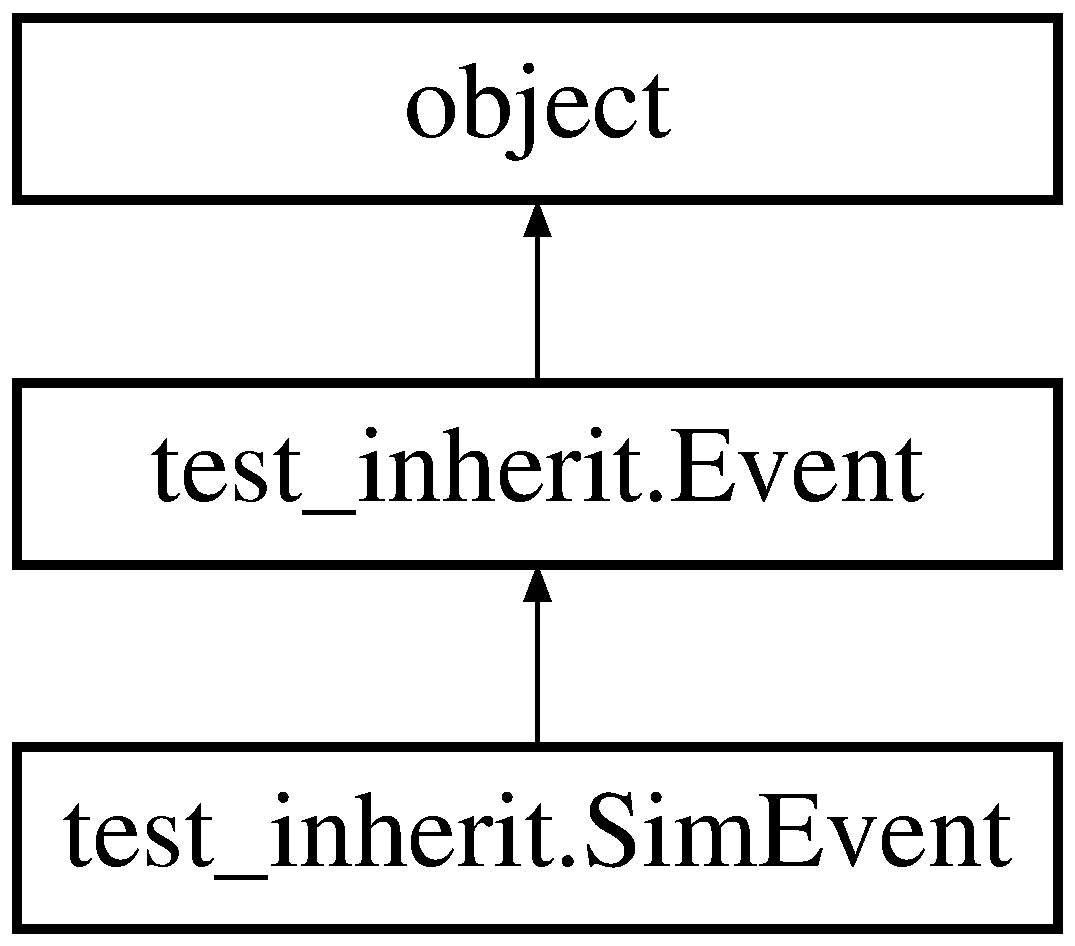
\includegraphics[height=3.000000cm]{da/db5/classtest__inherit_1_1_event}
\end{center}
\end{figure}
\subsection*{Public Member Functions}
\begin{DoxyCompactItemize}
\item 
def \hyperlink{classtest__inherit_1_1_event_ac1a0c9e92e19c1f9fd5e01d61947d05f}{\-\_\-\-\_\-init\-\_\-\-\_\-}
\item 
def \hyperlink{classtest__inherit_1_1_event_a724b1466524a0496c603051d8cfa1103}{\-\_\-\-\_\-del\-\_\-\-\_\-}
\item 
def \hyperlink{classtest__inherit_1_1_event_a36aa7bde7252d55aa750aab1a99e082b}{datetime}
\item 
def \hyperlink{classtest__inherit_1_1_event_a36aa7bde7252d55aa750aab1a99e082b}{datetime}
\item 
def \hyperlink{classtest__inherit_1_1_event_a36aa7bde7252d55aa750aab1a99e082b}{datetime}
\item 
def \hyperlink{classtest__inherit_1_1_event_a612fca9f9bff0c8a94f50f6651734554}{R\-A}
\item 
def \hyperlink{classtest__inherit_1_1_event_a612fca9f9bff0c8a94f50f6651734554}{R\-A}
\item 
def \hyperlink{classtest__inherit_1_1_event_a612fca9f9bff0c8a94f50f6651734554}{R\-A}
\item 
def \hyperlink{classtest__inherit_1_1_event_a55b4bedbc886eb77cfac7771850362ed}{dec}
\item 
def \hyperlink{classtest__inherit_1_1_event_a55b4bedbc886eb77cfac7771850362ed}{dec}
\item 
def \hyperlink{classtest__inherit_1_1_event_a55b4bedbc886eb77cfac7771850362ed}{dec}
\item 
def \hyperlink{classtest__inherit_1_1_event_a49b568e72d6286dc6902f657942031ac}{sigma\-R}
\item 
def \hyperlink{classtest__inherit_1_1_event_a49b568e72d6286dc6902f657942031ac}{sigma\-R}
\item 
def \hyperlink{classtest__inherit_1_1_event_a49b568e72d6286dc6902f657942031ac}{sigma\-R}
\item 
def \hyperlink{classtest__inherit_1_1_event_aa3d666daea0992b79fac728a2220a375}{nevents}
\item 
def \hyperlink{classtest__inherit_1_1_event_aa3d666daea0992b79fac728a2220a375}{nevents}
\item 
def \hyperlink{classtest__inherit_1_1_event_aa3d666daea0992b79fac728a2220a375}{nevents}
\item 
def \hyperlink{classtest__inherit_1_1_event_ab6d25d3eb1b861e9adda4318a2338eb8}{delta\-T}
\item 
def \hyperlink{classtest__inherit_1_1_event_ab6d25d3eb1b861e9adda4318a2338eb8}{delta\-T}
\item 
def \hyperlink{classtest__inherit_1_1_event_ab6d25d3eb1b861e9adda4318a2338eb8}{delta\-T}
\item 
def \hyperlink{classtest__inherit_1_1_event_a971807c984e01f2108809dea47a974ed}{sigma\-T}
\item 
def \hyperlink{classtest__inherit_1_1_event_a971807c984e01f2108809dea47a974ed}{sigma\-T}
\item 
def \hyperlink{classtest__inherit_1_1_event_a971807c984e01f2108809dea47a974ed}{sigma\-T}
\item 
def \hyperlink{classtest__inherit_1_1_event_aee2cdf46f225c1b0a25facd9bf113900}{false\-\_\-pos}
\item 
def \hyperlink{classtest__inherit_1_1_event_aee2cdf46f225c1b0a25facd9bf113900}{false\-\_\-pos}
\item 
def \hyperlink{classtest__inherit_1_1_event_aee2cdf46f225c1b0a25facd9bf113900}{false\-\_\-pos}
\item 
def \hyperlink{classtest__inherit_1_1_event_a0234c0de6ec72cafef67f6851b8a2b02}{pvalue}
\item 
def \hyperlink{classtest__inherit_1_1_event_a0234c0de6ec72cafef67f6851b8a2b02}{pvalue}
\item 
def \hyperlink{classtest__inherit_1_1_event_a0234c0de6ec72cafef67f6851b8a2b02}{pvalue}
\item 
def \hyperlink{classtest__inherit_1_1_event_a0b9bbf1d1069d9cbf6b94b7d55fdae50}{observing}
\item 
def \hyperlink{classtest__inherit_1_1_event_a0b9bbf1d1069d9cbf6b94b7d55fdae50}{observing}
\item 
def \hyperlink{classtest__inherit_1_1_event_a0b9bbf1d1069d9cbf6b94b7d55fdae50}{observing}
\item 
def \hyperlink{classtest__inherit_1_1_event_a0068a92b87d62915ada86852ba0ffa62}{trigger}
\item 
def \hyperlink{classtest__inherit_1_1_event_a0068a92b87d62915ada86852ba0ffa62}{trigger}
\item 
def \hyperlink{classtest__inherit_1_1_event_a0068a92b87d62915ada86852ba0ffa62}{trigger}
\item 
def \hyperlink{classtest__inherit_1_1_event_a32554137bdff7950f26ac803f1570655}{type}
\item 
def \hyperlink{classtest__inherit_1_1_event_a32554137bdff7950f26ac803f1570655}{type}
\item 
def \hyperlink{classtest__inherit_1_1_event_a32554137bdff7950f26ac803f1570655}{type}
\item 
def \hyperlink{classtest__inherit_1_1_event_a649f2803299a969f2baff16cd06ee184}{point\-\_\-\-R\-A}
\item 
def \hyperlink{classtest__inherit_1_1_event_a649f2803299a969f2baff16cd06ee184}{point\-\_\-\-R\-A}
\item 
def \hyperlink{classtest__inherit_1_1_event_a649f2803299a969f2baff16cd06ee184}{point\-\_\-\-R\-A}
\item 
def \hyperlink{classtest__inherit_1_1_event_a542fa880b2df3a8ebc14c8b091756b61}{point\-\_\-dec}
\item 
def \hyperlink{classtest__inherit_1_1_event_a542fa880b2df3a8ebc14c8b091756b61}{point\-\_\-dec}
\item 
def \hyperlink{classtest__inherit_1_1_event_a542fa880b2df3a8ebc14c8b091756b61}{point\-\_\-dec}
\item 
def \hyperlink{classtest__inherit_1_1_event_aa1e582bd70aa55f169b82d9485834f3b}{longitude}
\item 
def \hyperlink{classtest__inherit_1_1_event_aa1e582bd70aa55f169b82d9485834f3b}{longitude}
\item 
def \hyperlink{classtest__inherit_1_1_event_aa1e582bd70aa55f169b82d9485834f3b}{longitude}
\item 
def \hyperlink{classtest__inherit_1_1_event_a561ec644ae1652784a8dc0423c86a7bf}{latitude}
\item 
def \hyperlink{classtest__inherit_1_1_event_a561ec644ae1652784a8dc0423c86a7bf}{latitude}
\item 
def \hyperlink{classtest__inherit_1_1_event_a561ec644ae1652784a8dc0423c86a7bf}{latitude}
\item 
def \hyperlink{classtest__inherit_1_1_event_aa549a6580e8b50e59dcd3f7c18d3b61f}{elevation}
\item 
def \hyperlink{classtest__inherit_1_1_event_aa549a6580e8b50e59dcd3f7c18d3b61f}{elevation}
\item 
def \hyperlink{classtest__inherit_1_1_event_aa549a6580e8b50e59dcd3f7c18d3b61f}{elevation}
\item 
def \hyperlink{classtest__inherit_1_1_event_a6e70e8535119bfce20735f0b8a869162}{skymap}
\item 
def \hyperlink{classtest__inherit_1_1_event_a6e70e8535119bfce20735f0b8a869162}{skymap}
\item 
def \hyperlink{classtest__inherit_1_1_event_a6e70e8535119bfce20735f0b8a869162}{skymap}
\end{DoxyCompactItemize}
\subsection*{Public Attributes}
\begin{DoxyCompactItemize}
\item 
\hyperlink{classtest__inherit_1_1_event_a38bfcd2b6a2b6a68b7146c698dd67f7b}{stream}
\item 
\hyperlink{classtest__inherit_1_1_event_ad776b91acd2cdadf7e56b0eae0defb55}{id}
\item 
\hyperlink{classtest__inherit_1_1_event_a3332478f94ada42bc86e88b92bd90da2}{rev}
\end{DoxyCompactItemize}


\subsection{Detailed Description}
\hyperlink{classtest__inherit_1_1_event}{Event} class \#\#\#\#\#\#\#. 

Definition at line 10 of file test\-\_\-inherit.\-py.



\subsection{Constructor \& Destructor Documentation}
\hypertarget{classtest__inherit_1_1_event_ac1a0c9e92e19c1f9fd5e01d61947d05f}{\index{test\-\_\-inherit\-::\-Event@{test\-\_\-inherit\-::\-Event}!\-\_\-\-\_\-init\-\_\-\-\_\-@{\-\_\-\-\_\-init\-\_\-\-\_\-}}
\index{\-\_\-\-\_\-init\-\_\-\-\_\-@{\-\_\-\-\_\-init\-\_\-\-\_\-}!test_inherit::Event@{test\-\_\-inherit\-::\-Event}}
\subsubsection[{\-\_\-\-\_\-init\-\_\-\-\_\-}]{\setlength{\rightskip}{0pt plus 5cm}def test\-\_\-inherit.\-Event.\-\_\-\-\_\-init\-\_\-\-\_\- (
\begin{DoxyParamCaption}
\item[{}]{self, }
\item[{}]{stream, }
\item[{}]{id, }
\item[{}]{rev}
\end{DoxyParamCaption}
)}}\label{classtest__inherit_1_1_event_ac1a0c9e92e19c1f9fd5e01d61947d05f}


Definition at line 20 of file test\-\_\-inherit.\-py.

\hypertarget{classtest__inherit_1_1_event_a724b1466524a0496c603051d8cfa1103}{\index{test\-\_\-inherit\-::\-Event@{test\-\_\-inherit\-::\-Event}!\-\_\-\-\_\-del\-\_\-\-\_\-@{\-\_\-\-\_\-del\-\_\-\-\_\-}}
\index{\-\_\-\-\_\-del\-\_\-\-\_\-@{\-\_\-\-\_\-del\-\_\-\-\_\-}!test_inherit::Event@{test\-\_\-inherit\-::\-Event}}
\subsubsection[{\-\_\-\-\_\-del\-\_\-\-\_\-}]{\setlength{\rightskip}{0pt plus 5cm}def test\-\_\-inherit.\-Event.\-\_\-\-\_\-del\-\_\-\-\_\- (
\begin{DoxyParamCaption}
\item[{}]{self}
\end{DoxyParamCaption}
)}}\label{classtest__inherit_1_1_event_a724b1466524a0496c603051d8cfa1103}


Definition at line 48 of file test\-\_\-inherit.\-py.



\subsection{Member Function Documentation}
\hypertarget{classtest__inherit_1_1_event_a36aa7bde7252d55aa750aab1a99e082b}{\index{test\-\_\-inherit\-::\-Event@{test\-\_\-inherit\-::\-Event}!datetime@{datetime}}
\index{datetime@{datetime}!test_inherit::Event@{test\-\_\-inherit\-::\-Event}}
\subsubsection[{datetime}]{\setlength{\rightskip}{0pt plus 5cm}def test\-\_\-inherit.\-Event.\-datetime (
\begin{DoxyParamCaption}
\item[{}]{self}
\end{DoxyParamCaption}
)}}\label{classtest__inherit_1_1_event_a36aa7bde7252d55aa750aab1a99e082b}


Definition at line 55 of file test\-\_\-inherit.\-py.

\hypertarget{classtest__inherit_1_1_event_a36aa7bde7252d55aa750aab1a99e082b}{\index{test\-\_\-inherit\-::\-Event@{test\-\_\-inherit\-::\-Event}!datetime@{datetime}}
\index{datetime@{datetime}!test_inherit::Event@{test\-\_\-inherit\-::\-Event}}
\subsubsection[{datetime}]{\setlength{\rightskip}{0pt plus 5cm}def test\-\_\-inherit.\-Event.\-datetime (
\begin{DoxyParamCaption}
\item[{}]{self, }
\item[{}]{value}
\end{DoxyParamCaption}
)}}\label{classtest__inherit_1_1_event_a36aa7bde7252d55aa750aab1a99e082b}


Definition at line 58 of file test\-\_\-inherit.\-py.

\hypertarget{classtest__inherit_1_1_event_a36aa7bde7252d55aa750aab1a99e082b}{\index{test\-\_\-inherit\-::\-Event@{test\-\_\-inherit\-::\-Event}!datetime@{datetime}}
\index{datetime@{datetime}!test_inherit::Event@{test\-\_\-inherit\-::\-Event}}
\subsubsection[{datetime}]{\setlength{\rightskip}{0pt plus 5cm}def test\-\_\-inherit.\-Event.\-datetime (
\begin{DoxyParamCaption}
\item[{}]{self}
\end{DoxyParamCaption}
)}}\label{classtest__inherit_1_1_event_a36aa7bde7252d55aa750aab1a99e082b}


Definition at line 61 of file test\-\_\-inherit.\-py.

\hypertarget{classtest__inherit_1_1_event_a55b4bedbc886eb77cfac7771850362ed}{\index{test\-\_\-inherit\-::\-Event@{test\-\_\-inherit\-::\-Event}!dec@{dec}}
\index{dec@{dec}!test_inherit::Event@{test\-\_\-inherit\-::\-Event}}
\subsubsection[{dec}]{\setlength{\rightskip}{0pt plus 5cm}def test\-\_\-inherit.\-Event.\-dec (
\begin{DoxyParamCaption}
\item[{}]{self}
\end{DoxyParamCaption}
)}}\label{classtest__inherit_1_1_event_a55b4bedbc886eb77cfac7771850362ed}


Definition at line 75 of file test\-\_\-inherit.\-py.

\hypertarget{classtest__inherit_1_1_event_a55b4bedbc886eb77cfac7771850362ed}{\index{test\-\_\-inherit\-::\-Event@{test\-\_\-inherit\-::\-Event}!dec@{dec}}
\index{dec@{dec}!test_inherit::Event@{test\-\_\-inherit\-::\-Event}}
\subsubsection[{dec}]{\setlength{\rightskip}{0pt plus 5cm}def test\-\_\-inherit.\-Event.\-dec (
\begin{DoxyParamCaption}
\item[{}]{self, }
\item[{}]{value}
\end{DoxyParamCaption}
)}}\label{classtest__inherit_1_1_event_a55b4bedbc886eb77cfac7771850362ed}


Definition at line 78 of file test\-\_\-inherit.\-py.

\hypertarget{classtest__inherit_1_1_event_a55b4bedbc886eb77cfac7771850362ed}{\index{test\-\_\-inherit\-::\-Event@{test\-\_\-inherit\-::\-Event}!dec@{dec}}
\index{dec@{dec}!test_inherit::Event@{test\-\_\-inherit\-::\-Event}}
\subsubsection[{dec}]{\setlength{\rightskip}{0pt plus 5cm}def test\-\_\-inherit.\-Event.\-dec (
\begin{DoxyParamCaption}
\item[{}]{self}
\end{DoxyParamCaption}
)}}\label{classtest__inherit_1_1_event_a55b4bedbc886eb77cfac7771850362ed}


Definition at line 81 of file test\-\_\-inherit.\-py.

\hypertarget{classtest__inherit_1_1_event_ab6d25d3eb1b861e9adda4318a2338eb8}{\index{test\-\_\-inherit\-::\-Event@{test\-\_\-inherit\-::\-Event}!delta\-T@{delta\-T}}
\index{delta\-T@{delta\-T}!test_inherit::Event@{test\-\_\-inherit\-::\-Event}}
\subsubsection[{delta\-T}]{\setlength{\rightskip}{0pt plus 5cm}def test\-\_\-inherit.\-Event.\-delta\-T (
\begin{DoxyParamCaption}
\item[{}]{self}
\end{DoxyParamCaption}
)}}\label{classtest__inherit_1_1_event_ab6d25d3eb1b861e9adda4318a2338eb8}


Definition at line 105 of file test\-\_\-inherit.\-py.

\hypertarget{classtest__inherit_1_1_event_ab6d25d3eb1b861e9adda4318a2338eb8}{\index{test\-\_\-inherit\-::\-Event@{test\-\_\-inherit\-::\-Event}!delta\-T@{delta\-T}}
\index{delta\-T@{delta\-T}!test_inherit::Event@{test\-\_\-inherit\-::\-Event}}
\subsubsection[{delta\-T}]{\setlength{\rightskip}{0pt plus 5cm}def test\-\_\-inherit.\-Event.\-delta\-T (
\begin{DoxyParamCaption}
\item[{}]{self, }
\item[{}]{value}
\end{DoxyParamCaption}
)}}\label{classtest__inherit_1_1_event_ab6d25d3eb1b861e9adda4318a2338eb8}


Definition at line 108 of file test\-\_\-inherit.\-py.

\hypertarget{classtest__inherit_1_1_event_ab6d25d3eb1b861e9adda4318a2338eb8}{\index{test\-\_\-inherit\-::\-Event@{test\-\_\-inherit\-::\-Event}!delta\-T@{delta\-T}}
\index{delta\-T@{delta\-T}!test_inherit::Event@{test\-\_\-inherit\-::\-Event}}
\subsubsection[{delta\-T}]{\setlength{\rightskip}{0pt plus 5cm}def test\-\_\-inherit.\-Event.\-delta\-T (
\begin{DoxyParamCaption}
\item[{}]{self}
\end{DoxyParamCaption}
)}}\label{classtest__inherit_1_1_event_ab6d25d3eb1b861e9adda4318a2338eb8}


Definition at line 111 of file test\-\_\-inherit.\-py.

\hypertarget{classtest__inherit_1_1_event_aa549a6580e8b50e59dcd3f7c18d3b61f}{\index{test\-\_\-inherit\-::\-Event@{test\-\_\-inherit\-::\-Event}!elevation@{elevation}}
\index{elevation@{elevation}!test_inherit::Event@{test\-\_\-inherit\-::\-Event}}
\subsubsection[{elevation}]{\setlength{\rightskip}{0pt plus 5cm}def test\-\_\-inherit.\-Event.\-elevation (
\begin{DoxyParamCaption}
\item[{}]{self}
\end{DoxyParamCaption}
)}}\label{classtest__inherit_1_1_event_aa549a6580e8b50e59dcd3f7c18d3b61f}


Definition at line 215 of file test\-\_\-inherit.\-py.

\hypertarget{classtest__inherit_1_1_event_aa549a6580e8b50e59dcd3f7c18d3b61f}{\index{test\-\_\-inherit\-::\-Event@{test\-\_\-inherit\-::\-Event}!elevation@{elevation}}
\index{elevation@{elevation}!test_inherit::Event@{test\-\_\-inherit\-::\-Event}}
\subsubsection[{elevation}]{\setlength{\rightskip}{0pt plus 5cm}def test\-\_\-inherit.\-Event.\-elevation (
\begin{DoxyParamCaption}
\item[{}]{self, }
\item[{}]{value}
\end{DoxyParamCaption}
)}}\label{classtest__inherit_1_1_event_aa549a6580e8b50e59dcd3f7c18d3b61f}


Definition at line 218 of file test\-\_\-inherit.\-py.

\hypertarget{classtest__inherit_1_1_event_aa549a6580e8b50e59dcd3f7c18d3b61f}{\index{test\-\_\-inherit\-::\-Event@{test\-\_\-inherit\-::\-Event}!elevation@{elevation}}
\index{elevation@{elevation}!test_inherit::Event@{test\-\_\-inherit\-::\-Event}}
\subsubsection[{elevation}]{\setlength{\rightskip}{0pt plus 5cm}def test\-\_\-inherit.\-Event.\-elevation (
\begin{DoxyParamCaption}
\item[{}]{self}
\end{DoxyParamCaption}
)}}\label{classtest__inherit_1_1_event_aa549a6580e8b50e59dcd3f7c18d3b61f}


Definition at line 221 of file test\-\_\-inherit.\-py.

\hypertarget{classtest__inherit_1_1_event_aee2cdf46f225c1b0a25facd9bf113900}{\index{test\-\_\-inherit\-::\-Event@{test\-\_\-inherit\-::\-Event}!false\-\_\-pos@{false\-\_\-pos}}
\index{false\-\_\-pos@{false\-\_\-pos}!test_inherit::Event@{test\-\_\-inherit\-::\-Event}}
\subsubsection[{false\-\_\-pos}]{\setlength{\rightskip}{0pt plus 5cm}def test\-\_\-inherit.\-Event.\-false\-\_\-pos (
\begin{DoxyParamCaption}
\item[{}]{self}
\end{DoxyParamCaption}
)}}\label{classtest__inherit_1_1_event_aee2cdf46f225c1b0a25facd9bf113900}


Definition at line 125 of file test\-\_\-inherit.\-py.

\hypertarget{classtest__inherit_1_1_event_aee2cdf46f225c1b0a25facd9bf113900}{\index{test\-\_\-inherit\-::\-Event@{test\-\_\-inherit\-::\-Event}!false\-\_\-pos@{false\-\_\-pos}}
\index{false\-\_\-pos@{false\-\_\-pos}!test_inherit::Event@{test\-\_\-inherit\-::\-Event}}
\subsubsection[{false\-\_\-pos}]{\setlength{\rightskip}{0pt plus 5cm}def test\-\_\-inherit.\-Event.\-false\-\_\-pos (
\begin{DoxyParamCaption}
\item[{}]{self, }
\item[{}]{value}
\end{DoxyParamCaption}
)}}\label{classtest__inherit_1_1_event_aee2cdf46f225c1b0a25facd9bf113900}


Definition at line 128 of file test\-\_\-inherit.\-py.

\hypertarget{classtest__inherit_1_1_event_aee2cdf46f225c1b0a25facd9bf113900}{\index{test\-\_\-inherit\-::\-Event@{test\-\_\-inherit\-::\-Event}!false\-\_\-pos@{false\-\_\-pos}}
\index{false\-\_\-pos@{false\-\_\-pos}!test_inherit::Event@{test\-\_\-inherit\-::\-Event}}
\subsubsection[{false\-\_\-pos}]{\setlength{\rightskip}{0pt plus 5cm}def test\-\_\-inherit.\-Event.\-false\-\_\-pos (
\begin{DoxyParamCaption}
\item[{}]{self}
\end{DoxyParamCaption}
)}}\label{classtest__inherit_1_1_event_aee2cdf46f225c1b0a25facd9bf113900}


Definition at line 131 of file test\-\_\-inherit.\-py.

\hypertarget{classtest__inherit_1_1_event_a561ec644ae1652784a8dc0423c86a7bf}{\index{test\-\_\-inherit\-::\-Event@{test\-\_\-inherit\-::\-Event}!latitude@{latitude}}
\index{latitude@{latitude}!test_inherit::Event@{test\-\_\-inherit\-::\-Event}}
\subsubsection[{latitude}]{\setlength{\rightskip}{0pt plus 5cm}def test\-\_\-inherit.\-Event.\-latitude (
\begin{DoxyParamCaption}
\item[{}]{self}
\end{DoxyParamCaption}
)}}\label{classtest__inherit_1_1_event_a561ec644ae1652784a8dc0423c86a7bf}


Definition at line 205 of file test\-\_\-inherit.\-py.

\hypertarget{classtest__inherit_1_1_event_a561ec644ae1652784a8dc0423c86a7bf}{\index{test\-\_\-inherit\-::\-Event@{test\-\_\-inherit\-::\-Event}!latitude@{latitude}}
\index{latitude@{latitude}!test_inherit::Event@{test\-\_\-inherit\-::\-Event}}
\subsubsection[{latitude}]{\setlength{\rightskip}{0pt plus 5cm}def test\-\_\-inherit.\-Event.\-latitude (
\begin{DoxyParamCaption}
\item[{}]{self, }
\item[{}]{value}
\end{DoxyParamCaption}
)}}\label{classtest__inherit_1_1_event_a561ec644ae1652784a8dc0423c86a7bf}


Definition at line 208 of file test\-\_\-inherit.\-py.

\hypertarget{classtest__inherit_1_1_event_a561ec644ae1652784a8dc0423c86a7bf}{\index{test\-\_\-inherit\-::\-Event@{test\-\_\-inherit\-::\-Event}!latitude@{latitude}}
\index{latitude@{latitude}!test_inherit::Event@{test\-\_\-inherit\-::\-Event}}
\subsubsection[{latitude}]{\setlength{\rightskip}{0pt plus 5cm}def test\-\_\-inherit.\-Event.\-latitude (
\begin{DoxyParamCaption}
\item[{}]{self}
\end{DoxyParamCaption}
)}}\label{classtest__inherit_1_1_event_a561ec644ae1652784a8dc0423c86a7bf}


Definition at line 211 of file test\-\_\-inherit.\-py.

\hypertarget{classtest__inherit_1_1_event_aa1e582bd70aa55f169b82d9485834f3b}{\index{test\-\_\-inherit\-::\-Event@{test\-\_\-inherit\-::\-Event}!longitude@{longitude}}
\index{longitude@{longitude}!test_inherit::Event@{test\-\_\-inherit\-::\-Event}}
\subsubsection[{longitude}]{\setlength{\rightskip}{0pt plus 5cm}def test\-\_\-inherit.\-Event.\-longitude (
\begin{DoxyParamCaption}
\item[{}]{self}
\end{DoxyParamCaption}
)}}\label{classtest__inherit_1_1_event_aa1e582bd70aa55f169b82d9485834f3b}


Definition at line 195 of file test\-\_\-inherit.\-py.

\hypertarget{classtest__inherit_1_1_event_aa1e582bd70aa55f169b82d9485834f3b}{\index{test\-\_\-inherit\-::\-Event@{test\-\_\-inherit\-::\-Event}!longitude@{longitude}}
\index{longitude@{longitude}!test_inherit::Event@{test\-\_\-inherit\-::\-Event}}
\subsubsection[{longitude}]{\setlength{\rightskip}{0pt plus 5cm}def test\-\_\-inherit.\-Event.\-longitude (
\begin{DoxyParamCaption}
\item[{}]{self, }
\item[{}]{value}
\end{DoxyParamCaption}
)}}\label{classtest__inherit_1_1_event_aa1e582bd70aa55f169b82d9485834f3b}


Definition at line 198 of file test\-\_\-inherit.\-py.

\hypertarget{classtest__inherit_1_1_event_aa1e582bd70aa55f169b82d9485834f3b}{\index{test\-\_\-inherit\-::\-Event@{test\-\_\-inherit\-::\-Event}!longitude@{longitude}}
\index{longitude@{longitude}!test_inherit::Event@{test\-\_\-inherit\-::\-Event}}
\subsubsection[{longitude}]{\setlength{\rightskip}{0pt plus 5cm}def test\-\_\-inherit.\-Event.\-longitude (
\begin{DoxyParamCaption}
\item[{}]{self}
\end{DoxyParamCaption}
)}}\label{classtest__inherit_1_1_event_aa1e582bd70aa55f169b82d9485834f3b}


Definition at line 201 of file test\-\_\-inherit.\-py.

\hypertarget{classtest__inherit_1_1_event_aa3d666daea0992b79fac728a2220a375}{\index{test\-\_\-inherit\-::\-Event@{test\-\_\-inherit\-::\-Event}!nevents@{nevents}}
\index{nevents@{nevents}!test_inherit::Event@{test\-\_\-inherit\-::\-Event}}
\subsubsection[{nevents}]{\setlength{\rightskip}{0pt plus 5cm}def test\-\_\-inherit.\-Event.\-nevents (
\begin{DoxyParamCaption}
\item[{}]{self}
\end{DoxyParamCaption}
)}}\label{classtest__inherit_1_1_event_aa3d666daea0992b79fac728a2220a375}


Definition at line 95 of file test\-\_\-inherit.\-py.

\hypertarget{classtest__inherit_1_1_event_aa3d666daea0992b79fac728a2220a375}{\index{test\-\_\-inherit\-::\-Event@{test\-\_\-inherit\-::\-Event}!nevents@{nevents}}
\index{nevents@{nevents}!test_inherit::Event@{test\-\_\-inherit\-::\-Event}}
\subsubsection[{nevents}]{\setlength{\rightskip}{0pt plus 5cm}def test\-\_\-inherit.\-Event.\-nevents (
\begin{DoxyParamCaption}
\item[{}]{self, }
\item[{}]{value}
\end{DoxyParamCaption}
)}}\label{classtest__inherit_1_1_event_aa3d666daea0992b79fac728a2220a375}


Definition at line 98 of file test\-\_\-inherit.\-py.

\hypertarget{classtest__inherit_1_1_event_aa3d666daea0992b79fac728a2220a375}{\index{test\-\_\-inherit\-::\-Event@{test\-\_\-inherit\-::\-Event}!nevents@{nevents}}
\index{nevents@{nevents}!test_inherit::Event@{test\-\_\-inherit\-::\-Event}}
\subsubsection[{nevents}]{\setlength{\rightskip}{0pt plus 5cm}def test\-\_\-inherit.\-Event.\-nevents (
\begin{DoxyParamCaption}
\item[{}]{self}
\end{DoxyParamCaption}
)}}\label{classtest__inherit_1_1_event_aa3d666daea0992b79fac728a2220a375}


Definition at line 101 of file test\-\_\-inherit.\-py.

\hypertarget{classtest__inherit_1_1_event_a0b9bbf1d1069d9cbf6b94b7d55fdae50}{\index{test\-\_\-inherit\-::\-Event@{test\-\_\-inherit\-::\-Event}!observing@{observing}}
\index{observing@{observing}!test_inherit::Event@{test\-\_\-inherit\-::\-Event}}
\subsubsection[{observing}]{\setlength{\rightskip}{0pt plus 5cm}def test\-\_\-inherit.\-Event.\-observing (
\begin{DoxyParamCaption}
\item[{}]{self}
\end{DoxyParamCaption}
)}}\label{classtest__inherit_1_1_event_a0b9bbf1d1069d9cbf6b94b7d55fdae50}


Definition at line 145 of file test\-\_\-inherit.\-py.

\hypertarget{classtest__inherit_1_1_event_a0b9bbf1d1069d9cbf6b94b7d55fdae50}{\index{test\-\_\-inherit\-::\-Event@{test\-\_\-inherit\-::\-Event}!observing@{observing}}
\index{observing@{observing}!test_inherit::Event@{test\-\_\-inherit\-::\-Event}}
\subsubsection[{observing}]{\setlength{\rightskip}{0pt plus 5cm}def test\-\_\-inherit.\-Event.\-observing (
\begin{DoxyParamCaption}
\item[{}]{self, }
\item[{}]{value}
\end{DoxyParamCaption}
)}}\label{classtest__inherit_1_1_event_a0b9bbf1d1069d9cbf6b94b7d55fdae50}


Definition at line 148 of file test\-\_\-inherit.\-py.

\hypertarget{classtest__inherit_1_1_event_a0b9bbf1d1069d9cbf6b94b7d55fdae50}{\index{test\-\_\-inherit\-::\-Event@{test\-\_\-inherit\-::\-Event}!observing@{observing}}
\index{observing@{observing}!test_inherit::Event@{test\-\_\-inherit\-::\-Event}}
\subsubsection[{observing}]{\setlength{\rightskip}{0pt plus 5cm}def test\-\_\-inherit.\-Event.\-observing (
\begin{DoxyParamCaption}
\item[{}]{self}
\end{DoxyParamCaption}
)}}\label{classtest__inherit_1_1_event_a0b9bbf1d1069d9cbf6b94b7d55fdae50}


Definition at line 151 of file test\-\_\-inherit.\-py.

\hypertarget{classtest__inherit_1_1_event_a542fa880b2df3a8ebc14c8b091756b61}{\index{test\-\_\-inherit\-::\-Event@{test\-\_\-inherit\-::\-Event}!point\-\_\-dec@{point\-\_\-dec}}
\index{point\-\_\-dec@{point\-\_\-dec}!test_inherit::Event@{test\-\_\-inherit\-::\-Event}}
\subsubsection[{point\-\_\-dec}]{\setlength{\rightskip}{0pt plus 5cm}def test\-\_\-inherit.\-Event.\-point\-\_\-dec (
\begin{DoxyParamCaption}
\item[{}]{self}
\end{DoxyParamCaption}
)}}\label{classtest__inherit_1_1_event_a542fa880b2df3a8ebc14c8b091756b61}


Definition at line 185 of file test\-\_\-inherit.\-py.

\hypertarget{classtest__inherit_1_1_event_a542fa880b2df3a8ebc14c8b091756b61}{\index{test\-\_\-inherit\-::\-Event@{test\-\_\-inherit\-::\-Event}!point\-\_\-dec@{point\-\_\-dec}}
\index{point\-\_\-dec@{point\-\_\-dec}!test_inherit::Event@{test\-\_\-inherit\-::\-Event}}
\subsubsection[{point\-\_\-dec}]{\setlength{\rightskip}{0pt plus 5cm}def test\-\_\-inherit.\-Event.\-point\-\_\-dec (
\begin{DoxyParamCaption}
\item[{}]{self, }
\item[{}]{value}
\end{DoxyParamCaption}
)}}\label{classtest__inherit_1_1_event_a542fa880b2df3a8ebc14c8b091756b61}


Definition at line 188 of file test\-\_\-inherit.\-py.

\hypertarget{classtest__inherit_1_1_event_a542fa880b2df3a8ebc14c8b091756b61}{\index{test\-\_\-inherit\-::\-Event@{test\-\_\-inherit\-::\-Event}!point\-\_\-dec@{point\-\_\-dec}}
\index{point\-\_\-dec@{point\-\_\-dec}!test_inherit::Event@{test\-\_\-inherit\-::\-Event}}
\subsubsection[{point\-\_\-dec}]{\setlength{\rightskip}{0pt plus 5cm}def test\-\_\-inherit.\-Event.\-point\-\_\-dec (
\begin{DoxyParamCaption}
\item[{}]{self}
\end{DoxyParamCaption}
)}}\label{classtest__inherit_1_1_event_a542fa880b2df3a8ebc14c8b091756b61}


Definition at line 191 of file test\-\_\-inherit.\-py.

\hypertarget{classtest__inherit_1_1_event_a649f2803299a969f2baff16cd06ee184}{\index{test\-\_\-inherit\-::\-Event@{test\-\_\-inherit\-::\-Event}!point\-\_\-\-R\-A@{point\-\_\-\-R\-A}}
\index{point\-\_\-\-R\-A@{point\-\_\-\-R\-A}!test_inherit::Event@{test\-\_\-inherit\-::\-Event}}
\subsubsection[{point\-\_\-\-R\-A}]{\setlength{\rightskip}{0pt plus 5cm}def test\-\_\-inherit.\-Event.\-point\-\_\-\-R\-A (
\begin{DoxyParamCaption}
\item[{}]{self}
\end{DoxyParamCaption}
)}}\label{classtest__inherit_1_1_event_a649f2803299a969f2baff16cd06ee184}


Definition at line 175 of file test\-\_\-inherit.\-py.

\hypertarget{classtest__inherit_1_1_event_a649f2803299a969f2baff16cd06ee184}{\index{test\-\_\-inherit\-::\-Event@{test\-\_\-inherit\-::\-Event}!point\-\_\-\-R\-A@{point\-\_\-\-R\-A}}
\index{point\-\_\-\-R\-A@{point\-\_\-\-R\-A}!test_inherit::Event@{test\-\_\-inherit\-::\-Event}}
\subsubsection[{point\-\_\-\-R\-A}]{\setlength{\rightskip}{0pt plus 5cm}def test\-\_\-inherit.\-Event.\-point\-\_\-\-R\-A (
\begin{DoxyParamCaption}
\item[{}]{self, }
\item[{}]{value}
\end{DoxyParamCaption}
)}}\label{classtest__inherit_1_1_event_a649f2803299a969f2baff16cd06ee184}


Definition at line 178 of file test\-\_\-inherit.\-py.

\hypertarget{classtest__inherit_1_1_event_a649f2803299a969f2baff16cd06ee184}{\index{test\-\_\-inherit\-::\-Event@{test\-\_\-inherit\-::\-Event}!point\-\_\-\-R\-A@{point\-\_\-\-R\-A}}
\index{point\-\_\-\-R\-A@{point\-\_\-\-R\-A}!test_inherit::Event@{test\-\_\-inherit\-::\-Event}}
\subsubsection[{point\-\_\-\-R\-A}]{\setlength{\rightskip}{0pt plus 5cm}def test\-\_\-inherit.\-Event.\-point\-\_\-\-R\-A (
\begin{DoxyParamCaption}
\item[{}]{self}
\end{DoxyParamCaption}
)}}\label{classtest__inherit_1_1_event_a649f2803299a969f2baff16cd06ee184}


Definition at line 181 of file test\-\_\-inherit.\-py.

\hypertarget{classtest__inherit_1_1_event_a0234c0de6ec72cafef67f6851b8a2b02}{\index{test\-\_\-inherit\-::\-Event@{test\-\_\-inherit\-::\-Event}!pvalue@{pvalue}}
\index{pvalue@{pvalue}!test_inherit::Event@{test\-\_\-inherit\-::\-Event}}
\subsubsection[{pvalue}]{\setlength{\rightskip}{0pt plus 5cm}def test\-\_\-inherit.\-Event.\-pvalue (
\begin{DoxyParamCaption}
\item[{}]{self}
\end{DoxyParamCaption}
)}}\label{classtest__inherit_1_1_event_a0234c0de6ec72cafef67f6851b8a2b02}


Definition at line 135 of file test\-\_\-inherit.\-py.

\hypertarget{classtest__inherit_1_1_event_a0234c0de6ec72cafef67f6851b8a2b02}{\index{test\-\_\-inherit\-::\-Event@{test\-\_\-inherit\-::\-Event}!pvalue@{pvalue}}
\index{pvalue@{pvalue}!test_inherit::Event@{test\-\_\-inherit\-::\-Event}}
\subsubsection[{pvalue}]{\setlength{\rightskip}{0pt plus 5cm}def test\-\_\-inherit.\-Event.\-pvalue (
\begin{DoxyParamCaption}
\item[{}]{self, }
\item[{}]{value}
\end{DoxyParamCaption}
)}}\label{classtest__inherit_1_1_event_a0234c0de6ec72cafef67f6851b8a2b02}


Definition at line 138 of file test\-\_\-inherit.\-py.

\hypertarget{classtest__inherit_1_1_event_a0234c0de6ec72cafef67f6851b8a2b02}{\index{test\-\_\-inherit\-::\-Event@{test\-\_\-inherit\-::\-Event}!pvalue@{pvalue}}
\index{pvalue@{pvalue}!test_inherit::Event@{test\-\_\-inherit\-::\-Event}}
\subsubsection[{pvalue}]{\setlength{\rightskip}{0pt plus 5cm}def test\-\_\-inherit.\-Event.\-pvalue (
\begin{DoxyParamCaption}
\item[{}]{self}
\end{DoxyParamCaption}
)}}\label{classtest__inherit_1_1_event_a0234c0de6ec72cafef67f6851b8a2b02}


Definition at line 141 of file test\-\_\-inherit.\-py.

\hypertarget{classtest__inherit_1_1_event_a612fca9f9bff0c8a94f50f6651734554}{\index{test\-\_\-inherit\-::\-Event@{test\-\_\-inherit\-::\-Event}!R\-A@{R\-A}}
\index{R\-A@{R\-A}!test_inherit::Event@{test\-\_\-inherit\-::\-Event}}
\subsubsection[{R\-A}]{\setlength{\rightskip}{0pt plus 5cm}def test\-\_\-inherit.\-Event.\-R\-A (
\begin{DoxyParamCaption}
\item[{}]{self}
\end{DoxyParamCaption}
)}}\label{classtest__inherit_1_1_event_a612fca9f9bff0c8a94f50f6651734554}


Definition at line 65 of file test\-\_\-inherit.\-py.

\hypertarget{classtest__inherit_1_1_event_a612fca9f9bff0c8a94f50f6651734554}{\index{test\-\_\-inherit\-::\-Event@{test\-\_\-inherit\-::\-Event}!R\-A@{R\-A}}
\index{R\-A@{R\-A}!test_inherit::Event@{test\-\_\-inherit\-::\-Event}}
\subsubsection[{R\-A}]{\setlength{\rightskip}{0pt plus 5cm}def test\-\_\-inherit.\-Event.\-R\-A (
\begin{DoxyParamCaption}
\item[{}]{self, }
\item[{}]{value}
\end{DoxyParamCaption}
)}}\label{classtest__inherit_1_1_event_a612fca9f9bff0c8a94f50f6651734554}


Definition at line 68 of file test\-\_\-inherit.\-py.

\hypertarget{classtest__inherit_1_1_event_a612fca9f9bff0c8a94f50f6651734554}{\index{test\-\_\-inherit\-::\-Event@{test\-\_\-inherit\-::\-Event}!R\-A@{R\-A}}
\index{R\-A@{R\-A}!test_inherit::Event@{test\-\_\-inherit\-::\-Event}}
\subsubsection[{R\-A}]{\setlength{\rightskip}{0pt plus 5cm}def test\-\_\-inherit.\-Event.\-R\-A (
\begin{DoxyParamCaption}
\item[{}]{self}
\end{DoxyParamCaption}
)}}\label{classtest__inherit_1_1_event_a612fca9f9bff0c8a94f50f6651734554}


Definition at line 71 of file test\-\_\-inherit.\-py.

\hypertarget{classtest__inherit_1_1_event_a49b568e72d6286dc6902f657942031ac}{\index{test\-\_\-inherit\-::\-Event@{test\-\_\-inherit\-::\-Event}!sigma\-R@{sigma\-R}}
\index{sigma\-R@{sigma\-R}!test_inherit::Event@{test\-\_\-inherit\-::\-Event}}
\subsubsection[{sigma\-R}]{\setlength{\rightskip}{0pt plus 5cm}def test\-\_\-inherit.\-Event.\-sigma\-R (
\begin{DoxyParamCaption}
\item[{}]{self}
\end{DoxyParamCaption}
)}}\label{classtest__inherit_1_1_event_a49b568e72d6286dc6902f657942031ac}


Definition at line 85 of file test\-\_\-inherit.\-py.

\hypertarget{classtest__inherit_1_1_event_a49b568e72d6286dc6902f657942031ac}{\index{test\-\_\-inherit\-::\-Event@{test\-\_\-inherit\-::\-Event}!sigma\-R@{sigma\-R}}
\index{sigma\-R@{sigma\-R}!test_inherit::Event@{test\-\_\-inherit\-::\-Event}}
\subsubsection[{sigma\-R}]{\setlength{\rightskip}{0pt plus 5cm}def test\-\_\-inherit.\-Event.\-sigma\-R (
\begin{DoxyParamCaption}
\item[{}]{self, }
\item[{}]{value}
\end{DoxyParamCaption}
)}}\label{classtest__inherit_1_1_event_a49b568e72d6286dc6902f657942031ac}


Definition at line 88 of file test\-\_\-inherit.\-py.

\hypertarget{classtest__inherit_1_1_event_a49b568e72d6286dc6902f657942031ac}{\index{test\-\_\-inherit\-::\-Event@{test\-\_\-inherit\-::\-Event}!sigma\-R@{sigma\-R}}
\index{sigma\-R@{sigma\-R}!test_inherit::Event@{test\-\_\-inherit\-::\-Event}}
\subsubsection[{sigma\-R}]{\setlength{\rightskip}{0pt plus 5cm}def test\-\_\-inherit.\-Event.\-sigma\-R (
\begin{DoxyParamCaption}
\item[{}]{self}
\end{DoxyParamCaption}
)}}\label{classtest__inherit_1_1_event_a49b568e72d6286dc6902f657942031ac}


Definition at line 91 of file test\-\_\-inherit.\-py.

\hypertarget{classtest__inherit_1_1_event_a971807c984e01f2108809dea47a974ed}{\index{test\-\_\-inherit\-::\-Event@{test\-\_\-inherit\-::\-Event}!sigma\-T@{sigma\-T}}
\index{sigma\-T@{sigma\-T}!test_inherit::Event@{test\-\_\-inherit\-::\-Event}}
\subsubsection[{sigma\-T}]{\setlength{\rightskip}{0pt plus 5cm}def test\-\_\-inherit.\-Event.\-sigma\-T (
\begin{DoxyParamCaption}
\item[{}]{self}
\end{DoxyParamCaption}
)}}\label{classtest__inherit_1_1_event_a971807c984e01f2108809dea47a974ed}


Definition at line 115 of file test\-\_\-inherit.\-py.

\hypertarget{classtest__inherit_1_1_event_a971807c984e01f2108809dea47a974ed}{\index{test\-\_\-inherit\-::\-Event@{test\-\_\-inherit\-::\-Event}!sigma\-T@{sigma\-T}}
\index{sigma\-T@{sigma\-T}!test_inherit::Event@{test\-\_\-inherit\-::\-Event}}
\subsubsection[{sigma\-T}]{\setlength{\rightskip}{0pt plus 5cm}def test\-\_\-inherit.\-Event.\-sigma\-T (
\begin{DoxyParamCaption}
\item[{}]{self, }
\item[{}]{value}
\end{DoxyParamCaption}
)}}\label{classtest__inherit_1_1_event_a971807c984e01f2108809dea47a974ed}


Definition at line 118 of file test\-\_\-inherit.\-py.

\hypertarget{classtest__inherit_1_1_event_a971807c984e01f2108809dea47a974ed}{\index{test\-\_\-inherit\-::\-Event@{test\-\_\-inherit\-::\-Event}!sigma\-T@{sigma\-T}}
\index{sigma\-T@{sigma\-T}!test_inherit::Event@{test\-\_\-inherit\-::\-Event}}
\subsubsection[{sigma\-T}]{\setlength{\rightskip}{0pt plus 5cm}def test\-\_\-inherit.\-Event.\-sigma\-T (
\begin{DoxyParamCaption}
\item[{}]{self}
\end{DoxyParamCaption}
)}}\label{classtest__inherit_1_1_event_a971807c984e01f2108809dea47a974ed}


Definition at line 121 of file test\-\_\-inherit.\-py.

\hypertarget{classtest__inherit_1_1_event_a6e70e8535119bfce20735f0b8a869162}{\index{test\-\_\-inherit\-::\-Event@{test\-\_\-inherit\-::\-Event}!skymap@{skymap}}
\index{skymap@{skymap}!test_inherit::Event@{test\-\_\-inherit\-::\-Event}}
\subsubsection[{skymap}]{\setlength{\rightskip}{0pt plus 5cm}def test\-\_\-inherit.\-Event.\-skymap (
\begin{DoxyParamCaption}
\item[{}]{self}
\end{DoxyParamCaption}
)}}\label{classtest__inherit_1_1_event_a6e70e8535119bfce20735f0b8a869162}


Definition at line 225 of file test\-\_\-inherit.\-py.

\hypertarget{classtest__inherit_1_1_event_a6e70e8535119bfce20735f0b8a869162}{\index{test\-\_\-inherit\-::\-Event@{test\-\_\-inherit\-::\-Event}!skymap@{skymap}}
\index{skymap@{skymap}!test_inherit::Event@{test\-\_\-inherit\-::\-Event}}
\subsubsection[{skymap}]{\setlength{\rightskip}{0pt plus 5cm}def test\-\_\-inherit.\-Event.\-skymap (
\begin{DoxyParamCaption}
\item[{}]{self, }
\item[{}]{value}
\end{DoxyParamCaption}
)}}\label{classtest__inherit_1_1_event_a6e70e8535119bfce20735f0b8a869162}


Definition at line 228 of file test\-\_\-inherit.\-py.

\hypertarget{classtest__inherit_1_1_event_a6e70e8535119bfce20735f0b8a869162}{\index{test\-\_\-inherit\-::\-Event@{test\-\_\-inherit\-::\-Event}!skymap@{skymap}}
\index{skymap@{skymap}!test_inherit::Event@{test\-\_\-inherit\-::\-Event}}
\subsubsection[{skymap}]{\setlength{\rightskip}{0pt plus 5cm}def test\-\_\-inherit.\-Event.\-skymap (
\begin{DoxyParamCaption}
\item[{}]{self}
\end{DoxyParamCaption}
)}}\label{classtest__inherit_1_1_event_a6e70e8535119bfce20735f0b8a869162}


Definition at line 231 of file test\-\_\-inherit.\-py.

\hypertarget{classtest__inherit_1_1_event_a0068a92b87d62915ada86852ba0ffa62}{\index{test\-\_\-inherit\-::\-Event@{test\-\_\-inherit\-::\-Event}!trigger@{trigger}}
\index{trigger@{trigger}!test_inherit::Event@{test\-\_\-inherit\-::\-Event}}
\subsubsection[{trigger}]{\setlength{\rightskip}{0pt plus 5cm}def test\-\_\-inherit.\-Event.\-trigger (
\begin{DoxyParamCaption}
\item[{}]{self}
\end{DoxyParamCaption}
)}}\label{classtest__inherit_1_1_event_a0068a92b87d62915ada86852ba0ffa62}


Definition at line 155 of file test\-\_\-inherit.\-py.

\hypertarget{classtest__inherit_1_1_event_a0068a92b87d62915ada86852ba0ffa62}{\index{test\-\_\-inherit\-::\-Event@{test\-\_\-inherit\-::\-Event}!trigger@{trigger}}
\index{trigger@{trigger}!test_inherit::Event@{test\-\_\-inherit\-::\-Event}}
\subsubsection[{trigger}]{\setlength{\rightskip}{0pt plus 5cm}def test\-\_\-inherit.\-Event.\-trigger (
\begin{DoxyParamCaption}
\item[{}]{self, }
\item[{}]{value}
\end{DoxyParamCaption}
)}}\label{classtest__inherit_1_1_event_a0068a92b87d62915ada86852ba0ffa62}


Definition at line 158 of file test\-\_\-inherit.\-py.

\hypertarget{classtest__inherit_1_1_event_a0068a92b87d62915ada86852ba0ffa62}{\index{test\-\_\-inherit\-::\-Event@{test\-\_\-inherit\-::\-Event}!trigger@{trigger}}
\index{trigger@{trigger}!test_inherit::Event@{test\-\_\-inherit\-::\-Event}}
\subsubsection[{trigger}]{\setlength{\rightskip}{0pt plus 5cm}def test\-\_\-inherit.\-Event.\-trigger (
\begin{DoxyParamCaption}
\item[{}]{self}
\end{DoxyParamCaption}
)}}\label{classtest__inherit_1_1_event_a0068a92b87d62915ada86852ba0ffa62}


Definition at line 161 of file test\-\_\-inherit.\-py.

\hypertarget{classtest__inherit_1_1_event_a32554137bdff7950f26ac803f1570655}{\index{test\-\_\-inherit\-::\-Event@{test\-\_\-inherit\-::\-Event}!type@{type}}
\index{type@{type}!test_inherit::Event@{test\-\_\-inherit\-::\-Event}}
\subsubsection[{type}]{\setlength{\rightskip}{0pt plus 5cm}def test\-\_\-inherit.\-Event.\-type (
\begin{DoxyParamCaption}
\item[{}]{self}
\end{DoxyParamCaption}
)}}\label{classtest__inherit_1_1_event_a32554137bdff7950f26ac803f1570655}


Definition at line 165 of file test\-\_\-inherit.\-py.

\hypertarget{classtest__inherit_1_1_event_a32554137bdff7950f26ac803f1570655}{\index{test\-\_\-inherit\-::\-Event@{test\-\_\-inherit\-::\-Event}!type@{type}}
\index{type@{type}!test_inherit::Event@{test\-\_\-inherit\-::\-Event}}
\subsubsection[{type}]{\setlength{\rightskip}{0pt plus 5cm}def test\-\_\-inherit.\-Event.\-type (
\begin{DoxyParamCaption}
\item[{}]{self, }
\item[{}]{value}
\end{DoxyParamCaption}
)}}\label{classtest__inherit_1_1_event_a32554137bdff7950f26ac803f1570655}


Definition at line 168 of file test\-\_\-inherit.\-py.

\hypertarget{classtest__inherit_1_1_event_a32554137bdff7950f26ac803f1570655}{\index{test\-\_\-inherit\-::\-Event@{test\-\_\-inherit\-::\-Event}!type@{type}}
\index{type@{type}!test_inherit::Event@{test\-\_\-inherit\-::\-Event}}
\subsubsection[{type}]{\setlength{\rightskip}{0pt plus 5cm}def test\-\_\-inherit.\-Event.\-type (
\begin{DoxyParamCaption}
\item[{}]{self}
\end{DoxyParamCaption}
)}}\label{classtest__inherit_1_1_event_a32554137bdff7950f26ac803f1570655}


Definition at line 171 of file test\-\_\-inherit.\-py.



\subsection{Member Data Documentation}
\hypertarget{classtest__inherit_1_1_event_ad776b91acd2cdadf7e56b0eae0defb55}{\index{test\-\_\-inherit\-::\-Event@{test\-\_\-inherit\-::\-Event}!id@{id}}
\index{id@{id}!test_inherit::Event@{test\-\_\-inherit\-::\-Event}}
\subsubsection[{id}]{\setlength{\rightskip}{0pt plus 5cm}test\-\_\-inherit.\-Event.\-id}}\label{classtest__inherit_1_1_event_ad776b91acd2cdadf7e56b0eae0defb55}


Definition at line 22 of file test\-\_\-inherit.\-py.

\hypertarget{classtest__inherit_1_1_event_a3332478f94ada42bc86e88b92bd90da2}{\index{test\-\_\-inherit\-::\-Event@{test\-\_\-inherit\-::\-Event}!rev@{rev}}
\index{rev@{rev}!test_inherit::Event@{test\-\_\-inherit\-::\-Event}}
\subsubsection[{rev}]{\setlength{\rightskip}{0pt plus 5cm}test\-\_\-inherit.\-Event.\-rev}}\label{classtest__inherit_1_1_event_a3332478f94ada42bc86e88b92bd90da2}


Definition at line 23 of file test\-\_\-inherit.\-py.

\hypertarget{classtest__inherit_1_1_event_a38bfcd2b6a2b6a68b7146c698dd67f7b}{\index{test\-\_\-inherit\-::\-Event@{test\-\_\-inherit\-::\-Event}!stream@{stream}}
\index{stream@{stream}!test_inherit::Event@{test\-\_\-inherit\-::\-Event}}
\subsubsection[{stream}]{\setlength{\rightskip}{0pt plus 5cm}test\-\_\-inherit.\-Event.\-stream}}\label{classtest__inherit_1_1_event_a38bfcd2b6a2b6a68b7146c698dd67f7b}


Definition at line 21 of file test\-\_\-inherit.\-py.



The documentation for this class was generated from the following file\-:\begin{DoxyCompactItemize}
\item 
amonpy/dev/\hyperlink{test__inherit_8py}{test\-\_\-inherit.\-py}\end{DoxyCompactItemize}

\hypertarget{classamonpy_1_1dbase_1_1db__classes_1_1_event_stream_config}{\section{amonpy.\-dbase.\-db\-\_\-classes.\-Event\-Stream\-Config Class Reference}
\label{classamonpy_1_1dbase_1_1db__classes_1_1_event_stream_config}\index{amonpy.\-dbase.\-db\-\_\-classes.\-Event\-Stream\-Config@{amonpy.\-dbase.\-db\-\_\-classes.\-Event\-Stream\-Config}}
}
Inheritance diagram for amonpy.\-dbase.\-db\-\_\-classes.\-Event\-Stream\-Config\-:\begin{figure}[H]
\begin{center}
\leavevmode
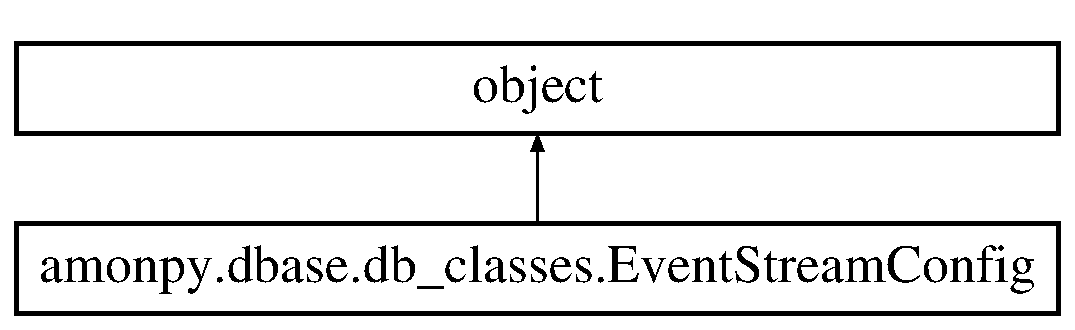
\includegraphics[height=2.000000cm]{classamonpy_1_1dbase_1_1db__classes_1_1_event_stream_config}
\end{center}
\end{figure}
\subsection*{Public Member Functions}
\begin{DoxyCompactItemize}
\item 
def \hyperlink{classamonpy_1_1dbase_1_1db__classes_1_1_event_stream_config_aeb56a654ef2b92bbeadf0bc5d43c4566}{\-\_\-\-\_\-init\-\_\-\-\_\-}
\item 
def \hyperlink{classamonpy_1_1dbase_1_1db__classes_1_1_event_stream_config_a713144a836f6d6853402597dc92eeec4}{\-\_\-\-\_\-del\-\_\-\-\_\-}
\item 
def \hyperlink{classamonpy_1_1dbase_1_1db__classes_1_1_event_stream_config_ad768b680b9b6e6b71b0b98cf5290c8fe}{duration}
\item 
def \hyperlink{classamonpy_1_1dbase_1_1db__classes_1_1_event_stream_config_a8b9de3b238c2062a10fad4b05b2290f2}{forprint}
\end{DoxyCompactItemize}
\subsection*{Public Attributes}
\begin{DoxyCompactItemize}
\item 
\hyperlink{classamonpy_1_1dbase_1_1db__classes_1_1_event_stream_config_a626d7977f5d3f63c3fbfb23d6b9716b3}{stream}
\item 
\hyperlink{classamonpy_1_1dbase_1_1db__classes_1_1_event_stream_config_af5e27bac4e9b5e18760ce85144f77bd4}{rev}
\item 
\hyperlink{classamonpy_1_1dbase_1_1db__classes_1_1_event_stream_config_a1736bfbecd4e57692307b26b11e85daf}{observ\-\_\-name}
\item 
\hyperlink{classamonpy_1_1dbase_1_1db__classes_1_1_event_stream_config_a92a9f0427f9d329992a04b077c311220}{valid\-Start}
\item 
\hyperlink{classamonpy_1_1dbase_1_1db__classes_1_1_event_stream_config_a55ef53af27e48c213db7b409c5459237}{valid\-Stop}
\item 
\hyperlink{classamonpy_1_1dbase_1_1db__classes_1_1_event_stream_config_ad7efccac3ae9b077bcc4d89595d82c08}{observ\-\_\-coord\-\_\-sys}
\item 
\hyperlink{classamonpy_1_1dbase_1_1db__classes_1_1_event_stream_config_aa3473b12a560dcab050cfe14e1edb203}{astro\-\_\-coord\-\_\-sys}
\item 
\hyperlink{classamonpy_1_1dbase_1_1db__classes_1_1_event_stream_config_a86e9966cac57a6aeddb4b6172ec1acfc}{point\-\_\-type}
\item 
\hyperlink{classamonpy_1_1dbase_1_1db__classes_1_1_event_stream_config_a138f290e26aa6b56d96f8b6bd9987b8f}{point}
\item 
\hyperlink{classamonpy_1_1dbase_1_1db__classes_1_1_event_stream_config_a2cc2e81b812c4e80b5d87779e1a320fe}{param1\-Desc}
\item 
\hyperlink{classamonpy_1_1dbase_1_1db__classes_1_1_event_stream_config_a1ac9462fd28120622b692b6db54521e0}{param2\-Desc}
\item 
\hyperlink{classamonpy_1_1dbase_1_1db__classes_1_1_event_stream_config_ac41f0f97661c293dce64bc89c8b9eade}{param3\-Desc}
\item 
\hyperlink{classamonpy_1_1dbase_1_1db__classes_1_1_event_stream_config_a9d8b36ab1042618f6e399a8f66b42118}{psf\-\_\-type}
\item 
\hyperlink{classamonpy_1_1dbase_1_1db__classes_1_1_event_stream_config_a12170d85350140f5fda128878d91277e}{psf}
\item 
\hyperlink{classamonpy_1_1dbase_1_1db__classes_1_1_event_stream_config_aaa2d6050a201048d2b2b16a4bb8faadb}{skymap\-\_\-val1\-Desc}
\item 
\hyperlink{classamonpy_1_1dbase_1_1db__classes_1_1_event_stream_config_a6db55d42905ecef2b4e46954edbab4d2}{skymap\-\_\-val2\-Desc}
\item 
\hyperlink{classamonpy_1_1dbase_1_1db__classes_1_1_event_stream_config_a017bb151fd3191f77338d6a9b78de0e2}{skymap\-\_\-val3\-Desc}
\item 
\hyperlink{classamonpy_1_1dbase_1_1db__classes_1_1_event_stream_config_afbac8232bbe89354fe55e04ae4864500}{sensitivity\-\_\-type}
\item 
\hyperlink{classamonpy_1_1dbase_1_1db__classes_1_1_event_stream_config_aff848f1925c8a6758214867b77689078}{sensitivity}
\item 
\hyperlink{classamonpy_1_1dbase_1_1db__classes_1_1_event_stream_config_aab09fd614aaa3622511e1602d11d3bd6}{fov\-\_\-type}
\item 
\hyperlink{classamonpy_1_1dbase_1_1db__classes_1_1_event_stream_config_a4c75df86251d603bf833057074b410da}{fov}
\item 
\hyperlink{classamonpy_1_1dbase_1_1db__classes_1_1_event_stream_config_a4b9131b75912c1e97f4e1b2b0402e4df}{ephemeris}
\item 
\hyperlink{classamonpy_1_1dbase_1_1db__classes_1_1_event_stream_config_a9d38a72e46882f06eb9e8a537e34148d}{bckgr\-\_\-type}
\item 
\hyperlink{classamonpy_1_1dbase_1_1db__classes_1_1_event_stream_config_a0914f43a8987820fafcb4eeffc1db845}{bckgr}
\item 
\hyperlink{classamonpy_1_1dbase_1_1db__classes_1_1_event_stream_config_ac3b7f4099b9bfeb3e80b20b842acdca6}{mag\-\_\-rigidity}
\end{DoxyCompactItemize}
\subsection*{Static Public Attributes}
\begin{DoxyCompactItemize}
\item 
int \hyperlink{classamonpy_1_1dbase_1_1db__classes_1_1_event_stream_config_a38d111218c593bec75f262725f91f5d2}{num\-\_\-configs} = 0
\end{DoxyCompactItemize}


\subsection{Detailed Description}
\begin{DoxyVerb}Creates the EventStreamConfig class. Instances are created by
    specifying a unique double of IDs (stream, rev). We use the same
    style of class definition as the Alert class
\end{DoxyVerb}
 

\subsection{Constructor \& Destructor Documentation}
\hypertarget{classamonpy_1_1dbase_1_1db__classes_1_1_event_stream_config_aeb56a654ef2b92bbeadf0bc5d43c4566}{\index{amonpy\-::dbase\-::db\-\_\-classes\-::\-Event\-Stream\-Config@{amonpy\-::dbase\-::db\-\_\-classes\-::\-Event\-Stream\-Config}!\-\_\-\-\_\-init\-\_\-\-\_\-@{\-\_\-\-\_\-init\-\_\-\-\_\-}}
\index{\-\_\-\-\_\-init\-\_\-\-\_\-@{\-\_\-\-\_\-init\-\_\-\-\_\-}!amonpy::dbase::db_classes::EventStreamConfig@{amonpy\-::dbase\-::db\-\_\-classes\-::\-Event\-Stream\-Config}}
\subsubsection[{\-\_\-\-\_\-init\-\_\-\-\_\-}]{\setlength{\rightskip}{0pt plus 5cm}def amonpy.\-dbase.\-db\-\_\-classes.\-Event\-Stream\-Config.\-\_\-\-\_\-init\-\_\-\-\_\- (
\begin{DoxyParamCaption}
\item[{}]{self, }
\item[{}]{stream, }
\item[{}]{rev}
\end{DoxyParamCaption}
)}}\label{classamonpy_1_1dbase_1_1db__classes_1_1_event_stream_config_aeb56a654ef2b92bbeadf0bc5d43c4566}
\hypertarget{classamonpy_1_1dbase_1_1db__classes_1_1_event_stream_config_a713144a836f6d6853402597dc92eeec4}{\index{amonpy\-::dbase\-::db\-\_\-classes\-::\-Event\-Stream\-Config@{amonpy\-::dbase\-::db\-\_\-classes\-::\-Event\-Stream\-Config}!\-\_\-\-\_\-del\-\_\-\-\_\-@{\-\_\-\-\_\-del\-\_\-\-\_\-}}
\index{\-\_\-\-\_\-del\-\_\-\-\_\-@{\-\_\-\-\_\-del\-\_\-\-\_\-}!amonpy::dbase::db_classes::EventStreamConfig@{amonpy\-::dbase\-::db\-\_\-classes\-::\-Event\-Stream\-Config}}
\subsubsection[{\-\_\-\-\_\-del\-\_\-\-\_\-}]{\setlength{\rightskip}{0pt plus 5cm}def amonpy.\-dbase.\-db\-\_\-classes.\-Event\-Stream\-Config.\-\_\-\-\_\-del\-\_\-\-\_\- (
\begin{DoxyParamCaption}
\item[{}]{self}
\end{DoxyParamCaption}
)}}\label{classamonpy_1_1dbase_1_1db__classes_1_1_event_stream_config_a713144a836f6d6853402597dc92eeec4}


\subsection{Member Function Documentation}
\hypertarget{classamonpy_1_1dbase_1_1db__classes_1_1_event_stream_config_ad768b680b9b6e6b71b0b98cf5290c8fe}{\index{amonpy\-::dbase\-::db\-\_\-classes\-::\-Event\-Stream\-Config@{amonpy\-::dbase\-::db\-\_\-classes\-::\-Event\-Stream\-Config}!duration@{duration}}
\index{duration@{duration}!amonpy::dbase::db_classes::EventStreamConfig@{amonpy\-::dbase\-::db\-\_\-classes\-::\-Event\-Stream\-Config}}
\subsubsection[{duration}]{\setlength{\rightskip}{0pt plus 5cm}def amonpy.\-dbase.\-db\-\_\-classes.\-Event\-Stream\-Config.\-duration (
\begin{DoxyParamCaption}
\item[{}]{self}
\end{DoxyParamCaption}
)}}\label{classamonpy_1_1dbase_1_1db__classes_1_1_event_stream_config_ad768b680b9b6e6b71b0b98cf5290c8fe}
\hypertarget{classamonpy_1_1dbase_1_1db__classes_1_1_event_stream_config_a8b9de3b238c2062a10fad4b05b2290f2}{\index{amonpy\-::dbase\-::db\-\_\-classes\-::\-Event\-Stream\-Config@{amonpy\-::dbase\-::db\-\_\-classes\-::\-Event\-Stream\-Config}!forprint@{forprint}}
\index{forprint@{forprint}!amonpy::dbase::db_classes::EventStreamConfig@{amonpy\-::dbase\-::db\-\_\-classes\-::\-Event\-Stream\-Config}}
\subsubsection[{forprint}]{\setlength{\rightskip}{0pt plus 5cm}def amonpy.\-dbase.\-db\-\_\-classes.\-Event\-Stream\-Config.\-forprint (
\begin{DoxyParamCaption}
\item[{}]{self}
\end{DoxyParamCaption}
)}}\label{classamonpy_1_1dbase_1_1db__classes_1_1_event_stream_config_a8b9de3b238c2062a10fad4b05b2290f2}


\subsection{Member Data Documentation}
\hypertarget{classamonpy_1_1dbase_1_1db__classes_1_1_event_stream_config_aa3473b12a560dcab050cfe14e1edb203}{\index{amonpy\-::dbase\-::db\-\_\-classes\-::\-Event\-Stream\-Config@{amonpy\-::dbase\-::db\-\_\-classes\-::\-Event\-Stream\-Config}!astro\-\_\-coord\-\_\-sys@{astro\-\_\-coord\-\_\-sys}}
\index{astro\-\_\-coord\-\_\-sys@{astro\-\_\-coord\-\_\-sys}!amonpy::dbase::db_classes::EventStreamConfig@{amonpy\-::dbase\-::db\-\_\-classes\-::\-Event\-Stream\-Config}}
\subsubsection[{astro\-\_\-coord\-\_\-sys}]{\setlength{\rightskip}{0pt plus 5cm}amonpy.\-dbase.\-db\-\_\-classes.\-Event\-Stream\-Config.\-astro\-\_\-coord\-\_\-sys}}\label{classamonpy_1_1dbase_1_1db__classes_1_1_event_stream_config_aa3473b12a560dcab050cfe14e1edb203}
\hypertarget{classamonpy_1_1dbase_1_1db__classes_1_1_event_stream_config_a0914f43a8987820fafcb4eeffc1db845}{\index{amonpy\-::dbase\-::db\-\_\-classes\-::\-Event\-Stream\-Config@{amonpy\-::dbase\-::db\-\_\-classes\-::\-Event\-Stream\-Config}!bckgr@{bckgr}}
\index{bckgr@{bckgr}!amonpy::dbase::db_classes::EventStreamConfig@{amonpy\-::dbase\-::db\-\_\-classes\-::\-Event\-Stream\-Config}}
\subsubsection[{bckgr}]{\setlength{\rightskip}{0pt plus 5cm}amonpy.\-dbase.\-db\-\_\-classes.\-Event\-Stream\-Config.\-bckgr}}\label{classamonpy_1_1dbase_1_1db__classes_1_1_event_stream_config_a0914f43a8987820fafcb4eeffc1db845}
\hypertarget{classamonpy_1_1dbase_1_1db__classes_1_1_event_stream_config_a9d38a72e46882f06eb9e8a537e34148d}{\index{amonpy\-::dbase\-::db\-\_\-classes\-::\-Event\-Stream\-Config@{amonpy\-::dbase\-::db\-\_\-classes\-::\-Event\-Stream\-Config}!bckgr\-\_\-type@{bckgr\-\_\-type}}
\index{bckgr\-\_\-type@{bckgr\-\_\-type}!amonpy::dbase::db_classes::EventStreamConfig@{amonpy\-::dbase\-::db\-\_\-classes\-::\-Event\-Stream\-Config}}
\subsubsection[{bckgr\-\_\-type}]{\setlength{\rightskip}{0pt plus 5cm}amonpy.\-dbase.\-db\-\_\-classes.\-Event\-Stream\-Config.\-bckgr\-\_\-type}}\label{classamonpy_1_1dbase_1_1db__classes_1_1_event_stream_config_a9d38a72e46882f06eb9e8a537e34148d}
\hypertarget{classamonpy_1_1dbase_1_1db__classes_1_1_event_stream_config_a4b9131b75912c1e97f4e1b2b0402e4df}{\index{amonpy\-::dbase\-::db\-\_\-classes\-::\-Event\-Stream\-Config@{amonpy\-::dbase\-::db\-\_\-classes\-::\-Event\-Stream\-Config}!ephemeris@{ephemeris}}
\index{ephemeris@{ephemeris}!amonpy::dbase::db_classes::EventStreamConfig@{amonpy\-::dbase\-::db\-\_\-classes\-::\-Event\-Stream\-Config}}
\subsubsection[{ephemeris}]{\setlength{\rightskip}{0pt plus 5cm}amonpy.\-dbase.\-db\-\_\-classes.\-Event\-Stream\-Config.\-ephemeris}}\label{classamonpy_1_1dbase_1_1db__classes_1_1_event_stream_config_a4b9131b75912c1e97f4e1b2b0402e4df}
\hypertarget{classamonpy_1_1dbase_1_1db__classes_1_1_event_stream_config_a4c75df86251d603bf833057074b410da}{\index{amonpy\-::dbase\-::db\-\_\-classes\-::\-Event\-Stream\-Config@{amonpy\-::dbase\-::db\-\_\-classes\-::\-Event\-Stream\-Config}!fov@{fov}}
\index{fov@{fov}!amonpy::dbase::db_classes::EventStreamConfig@{amonpy\-::dbase\-::db\-\_\-classes\-::\-Event\-Stream\-Config}}
\subsubsection[{fov}]{\setlength{\rightskip}{0pt plus 5cm}amonpy.\-dbase.\-db\-\_\-classes.\-Event\-Stream\-Config.\-fov}}\label{classamonpy_1_1dbase_1_1db__classes_1_1_event_stream_config_a4c75df86251d603bf833057074b410da}
\hypertarget{classamonpy_1_1dbase_1_1db__classes_1_1_event_stream_config_aab09fd614aaa3622511e1602d11d3bd6}{\index{amonpy\-::dbase\-::db\-\_\-classes\-::\-Event\-Stream\-Config@{amonpy\-::dbase\-::db\-\_\-classes\-::\-Event\-Stream\-Config}!fov\-\_\-type@{fov\-\_\-type}}
\index{fov\-\_\-type@{fov\-\_\-type}!amonpy::dbase::db_classes::EventStreamConfig@{amonpy\-::dbase\-::db\-\_\-classes\-::\-Event\-Stream\-Config}}
\subsubsection[{fov\-\_\-type}]{\setlength{\rightskip}{0pt plus 5cm}amonpy.\-dbase.\-db\-\_\-classes.\-Event\-Stream\-Config.\-fov\-\_\-type}}\label{classamonpy_1_1dbase_1_1db__classes_1_1_event_stream_config_aab09fd614aaa3622511e1602d11d3bd6}
\hypertarget{classamonpy_1_1dbase_1_1db__classes_1_1_event_stream_config_ac3b7f4099b9bfeb3e80b20b842acdca6}{\index{amonpy\-::dbase\-::db\-\_\-classes\-::\-Event\-Stream\-Config@{amonpy\-::dbase\-::db\-\_\-classes\-::\-Event\-Stream\-Config}!mag\-\_\-rigidity@{mag\-\_\-rigidity}}
\index{mag\-\_\-rigidity@{mag\-\_\-rigidity}!amonpy::dbase::db_classes::EventStreamConfig@{amonpy\-::dbase\-::db\-\_\-classes\-::\-Event\-Stream\-Config}}
\subsubsection[{mag\-\_\-rigidity}]{\setlength{\rightskip}{0pt plus 5cm}amonpy.\-dbase.\-db\-\_\-classes.\-Event\-Stream\-Config.\-mag\-\_\-rigidity}}\label{classamonpy_1_1dbase_1_1db__classes_1_1_event_stream_config_ac3b7f4099b9bfeb3e80b20b842acdca6}
\hypertarget{classamonpy_1_1dbase_1_1db__classes_1_1_event_stream_config_a38d111218c593bec75f262725f91f5d2}{\index{amonpy\-::dbase\-::db\-\_\-classes\-::\-Event\-Stream\-Config@{amonpy\-::dbase\-::db\-\_\-classes\-::\-Event\-Stream\-Config}!num\-\_\-configs@{num\-\_\-configs}}
\index{num\-\_\-configs@{num\-\_\-configs}!amonpy::dbase::db_classes::EventStreamConfig@{amonpy\-::dbase\-::db\-\_\-classes\-::\-Event\-Stream\-Config}}
\subsubsection[{num\-\_\-configs}]{\setlength{\rightskip}{0pt plus 5cm}int amonpy.\-dbase.\-db\-\_\-classes.\-Event\-Stream\-Config.\-num\-\_\-configs = 0\hspace{0.3cm}{\ttfamily [static]}}}\label{classamonpy_1_1dbase_1_1db__classes_1_1_event_stream_config_a38d111218c593bec75f262725f91f5d2}
\hypertarget{classamonpy_1_1dbase_1_1db__classes_1_1_event_stream_config_ad7efccac3ae9b077bcc4d89595d82c08}{\index{amonpy\-::dbase\-::db\-\_\-classes\-::\-Event\-Stream\-Config@{amonpy\-::dbase\-::db\-\_\-classes\-::\-Event\-Stream\-Config}!observ\-\_\-coord\-\_\-sys@{observ\-\_\-coord\-\_\-sys}}
\index{observ\-\_\-coord\-\_\-sys@{observ\-\_\-coord\-\_\-sys}!amonpy::dbase::db_classes::EventStreamConfig@{amonpy\-::dbase\-::db\-\_\-classes\-::\-Event\-Stream\-Config}}
\subsubsection[{observ\-\_\-coord\-\_\-sys}]{\setlength{\rightskip}{0pt plus 5cm}amonpy.\-dbase.\-db\-\_\-classes.\-Event\-Stream\-Config.\-observ\-\_\-coord\-\_\-sys}}\label{classamonpy_1_1dbase_1_1db__classes_1_1_event_stream_config_ad7efccac3ae9b077bcc4d89595d82c08}
\hypertarget{classamonpy_1_1dbase_1_1db__classes_1_1_event_stream_config_a1736bfbecd4e57692307b26b11e85daf}{\index{amonpy\-::dbase\-::db\-\_\-classes\-::\-Event\-Stream\-Config@{amonpy\-::dbase\-::db\-\_\-classes\-::\-Event\-Stream\-Config}!observ\-\_\-name@{observ\-\_\-name}}
\index{observ\-\_\-name@{observ\-\_\-name}!amonpy::dbase::db_classes::EventStreamConfig@{amonpy\-::dbase\-::db\-\_\-classes\-::\-Event\-Stream\-Config}}
\subsubsection[{observ\-\_\-name}]{\setlength{\rightskip}{0pt plus 5cm}amonpy.\-dbase.\-db\-\_\-classes.\-Event\-Stream\-Config.\-observ\-\_\-name}}\label{classamonpy_1_1dbase_1_1db__classes_1_1_event_stream_config_a1736bfbecd4e57692307b26b11e85daf}
\hypertarget{classamonpy_1_1dbase_1_1db__classes_1_1_event_stream_config_a2cc2e81b812c4e80b5d87779e1a320fe}{\index{amonpy\-::dbase\-::db\-\_\-classes\-::\-Event\-Stream\-Config@{amonpy\-::dbase\-::db\-\_\-classes\-::\-Event\-Stream\-Config}!param1\-Desc@{param1\-Desc}}
\index{param1\-Desc@{param1\-Desc}!amonpy::dbase::db_classes::EventStreamConfig@{amonpy\-::dbase\-::db\-\_\-classes\-::\-Event\-Stream\-Config}}
\subsubsection[{param1\-Desc}]{\setlength{\rightskip}{0pt plus 5cm}amonpy.\-dbase.\-db\-\_\-classes.\-Event\-Stream\-Config.\-param1\-Desc}}\label{classamonpy_1_1dbase_1_1db__classes_1_1_event_stream_config_a2cc2e81b812c4e80b5d87779e1a320fe}
\hypertarget{classamonpy_1_1dbase_1_1db__classes_1_1_event_stream_config_a1ac9462fd28120622b692b6db54521e0}{\index{amonpy\-::dbase\-::db\-\_\-classes\-::\-Event\-Stream\-Config@{amonpy\-::dbase\-::db\-\_\-classes\-::\-Event\-Stream\-Config}!param2\-Desc@{param2\-Desc}}
\index{param2\-Desc@{param2\-Desc}!amonpy::dbase::db_classes::EventStreamConfig@{amonpy\-::dbase\-::db\-\_\-classes\-::\-Event\-Stream\-Config}}
\subsubsection[{param2\-Desc}]{\setlength{\rightskip}{0pt plus 5cm}amonpy.\-dbase.\-db\-\_\-classes.\-Event\-Stream\-Config.\-param2\-Desc}}\label{classamonpy_1_1dbase_1_1db__classes_1_1_event_stream_config_a1ac9462fd28120622b692b6db54521e0}
\hypertarget{classamonpy_1_1dbase_1_1db__classes_1_1_event_stream_config_ac41f0f97661c293dce64bc89c8b9eade}{\index{amonpy\-::dbase\-::db\-\_\-classes\-::\-Event\-Stream\-Config@{amonpy\-::dbase\-::db\-\_\-classes\-::\-Event\-Stream\-Config}!param3\-Desc@{param3\-Desc}}
\index{param3\-Desc@{param3\-Desc}!amonpy::dbase::db_classes::EventStreamConfig@{amonpy\-::dbase\-::db\-\_\-classes\-::\-Event\-Stream\-Config}}
\subsubsection[{param3\-Desc}]{\setlength{\rightskip}{0pt plus 5cm}amonpy.\-dbase.\-db\-\_\-classes.\-Event\-Stream\-Config.\-param3\-Desc}}\label{classamonpy_1_1dbase_1_1db__classes_1_1_event_stream_config_ac41f0f97661c293dce64bc89c8b9eade}
\hypertarget{classamonpy_1_1dbase_1_1db__classes_1_1_event_stream_config_a138f290e26aa6b56d96f8b6bd9987b8f}{\index{amonpy\-::dbase\-::db\-\_\-classes\-::\-Event\-Stream\-Config@{amonpy\-::dbase\-::db\-\_\-classes\-::\-Event\-Stream\-Config}!point@{point}}
\index{point@{point}!amonpy::dbase::db_classes::EventStreamConfig@{amonpy\-::dbase\-::db\-\_\-classes\-::\-Event\-Stream\-Config}}
\subsubsection[{point}]{\setlength{\rightskip}{0pt plus 5cm}amonpy.\-dbase.\-db\-\_\-classes.\-Event\-Stream\-Config.\-point}}\label{classamonpy_1_1dbase_1_1db__classes_1_1_event_stream_config_a138f290e26aa6b56d96f8b6bd9987b8f}
\hypertarget{classamonpy_1_1dbase_1_1db__classes_1_1_event_stream_config_a86e9966cac57a6aeddb4b6172ec1acfc}{\index{amonpy\-::dbase\-::db\-\_\-classes\-::\-Event\-Stream\-Config@{amonpy\-::dbase\-::db\-\_\-classes\-::\-Event\-Stream\-Config}!point\-\_\-type@{point\-\_\-type}}
\index{point\-\_\-type@{point\-\_\-type}!amonpy::dbase::db_classes::EventStreamConfig@{amonpy\-::dbase\-::db\-\_\-classes\-::\-Event\-Stream\-Config}}
\subsubsection[{point\-\_\-type}]{\setlength{\rightskip}{0pt plus 5cm}amonpy.\-dbase.\-db\-\_\-classes.\-Event\-Stream\-Config.\-point\-\_\-type}}\label{classamonpy_1_1dbase_1_1db__classes_1_1_event_stream_config_a86e9966cac57a6aeddb4b6172ec1acfc}
\hypertarget{classamonpy_1_1dbase_1_1db__classes_1_1_event_stream_config_a12170d85350140f5fda128878d91277e}{\index{amonpy\-::dbase\-::db\-\_\-classes\-::\-Event\-Stream\-Config@{amonpy\-::dbase\-::db\-\_\-classes\-::\-Event\-Stream\-Config}!psf@{psf}}
\index{psf@{psf}!amonpy::dbase::db_classes::EventStreamConfig@{amonpy\-::dbase\-::db\-\_\-classes\-::\-Event\-Stream\-Config}}
\subsubsection[{psf}]{\setlength{\rightskip}{0pt plus 5cm}amonpy.\-dbase.\-db\-\_\-classes.\-Event\-Stream\-Config.\-psf}}\label{classamonpy_1_1dbase_1_1db__classes_1_1_event_stream_config_a12170d85350140f5fda128878d91277e}
\hypertarget{classamonpy_1_1dbase_1_1db__classes_1_1_event_stream_config_a9d8b36ab1042618f6e399a8f66b42118}{\index{amonpy\-::dbase\-::db\-\_\-classes\-::\-Event\-Stream\-Config@{amonpy\-::dbase\-::db\-\_\-classes\-::\-Event\-Stream\-Config}!psf\-\_\-type@{psf\-\_\-type}}
\index{psf\-\_\-type@{psf\-\_\-type}!amonpy::dbase::db_classes::EventStreamConfig@{amonpy\-::dbase\-::db\-\_\-classes\-::\-Event\-Stream\-Config}}
\subsubsection[{psf\-\_\-type}]{\setlength{\rightskip}{0pt plus 5cm}amonpy.\-dbase.\-db\-\_\-classes.\-Event\-Stream\-Config.\-psf\-\_\-type}}\label{classamonpy_1_1dbase_1_1db__classes_1_1_event_stream_config_a9d8b36ab1042618f6e399a8f66b42118}
\hypertarget{classamonpy_1_1dbase_1_1db__classes_1_1_event_stream_config_af5e27bac4e9b5e18760ce85144f77bd4}{\index{amonpy\-::dbase\-::db\-\_\-classes\-::\-Event\-Stream\-Config@{amonpy\-::dbase\-::db\-\_\-classes\-::\-Event\-Stream\-Config}!rev@{rev}}
\index{rev@{rev}!amonpy::dbase::db_classes::EventStreamConfig@{amonpy\-::dbase\-::db\-\_\-classes\-::\-Event\-Stream\-Config}}
\subsubsection[{rev}]{\setlength{\rightskip}{0pt plus 5cm}amonpy.\-dbase.\-db\-\_\-classes.\-Event\-Stream\-Config.\-rev}}\label{classamonpy_1_1dbase_1_1db__classes_1_1_event_stream_config_af5e27bac4e9b5e18760ce85144f77bd4}
\hypertarget{classamonpy_1_1dbase_1_1db__classes_1_1_event_stream_config_aff848f1925c8a6758214867b77689078}{\index{amonpy\-::dbase\-::db\-\_\-classes\-::\-Event\-Stream\-Config@{amonpy\-::dbase\-::db\-\_\-classes\-::\-Event\-Stream\-Config}!sensitivity@{sensitivity}}
\index{sensitivity@{sensitivity}!amonpy::dbase::db_classes::EventStreamConfig@{amonpy\-::dbase\-::db\-\_\-classes\-::\-Event\-Stream\-Config}}
\subsubsection[{sensitivity}]{\setlength{\rightskip}{0pt plus 5cm}amonpy.\-dbase.\-db\-\_\-classes.\-Event\-Stream\-Config.\-sensitivity}}\label{classamonpy_1_1dbase_1_1db__classes_1_1_event_stream_config_aff848f1925c8a6758214867b77689078}
\hypertarget{classamonpy_1_1dbase_1_1db__classes_1_1_event_stream_config_afbac8232bbe89354fe55e04ae4864500}{\index{amonpy\-::dbase\-::db\-\_\-classes\-::\-Event\-Stream\-Config@{amonpy\-::dbase\-::db\-\_\-classes\-::\-Event\-Stream\-Config}!sensitivity\-\_\-type@{sensitivity\-\_\-type}}
\index{sensitivity\-\_\-type@{sensitivity\-\_\-type}!amonpy::dbase::db_classes::EventStreamConfig@{amonpy\-::dbase\-::db\-\_\-classes\-::\-Event\-Stream\-Config}}
\subsubsection[{sensitivity\-\_\-type}]{\setlength{\rightskip}{0pt plus 5cm}amonpy.\-dbase.\-db\-\_\-classes.\-Event\-Stream\-Config.\-sensitivity\-\_\-type}}\label{classamonpy_1_1dbase_1_1db__classes_1_1_event_stream_config_afbac8232bbe89354fe55e04ae4864500}
\hypertarget{classamonpy_1_1dbase_1_1db__classes_1_1_event_stream_config_aaa2d6050a201048d2b2b16a4bb8faadb}{\index{amonpy\-::dbase\-::db\-\_\-classes\-::\-Event\-Stream\-Config@{amonpy\-::dbase\-::db\-\_\-classes\-::\-Event\-Stream\-Config}!skymap\-\_\-val1\-Desc@{skymap\-\_\-val1\-Desc}}
\index{skymap\-\_\-val1\-Desc@{skymap\-\_\-val1\-Desc}!amonpy::dbase::db_classes::EventStreamConfig@{amonpy\-::dbase\-::db\-\_\-classes\-::\-Event\-Stream\-Config}}
\subsubsection[{skymap\-\_\-val1\-Desc}]{\setlength{\rightskip}{0pt plus 5cm}amonpy.\-dbase.\-db\-\_\-classes.\-Event\-Stream\-Config.\-skymap\-\_\-val1\-Desc}}\label{classamonpy_1_1dbase_1_1db__classes_1_1_event_stream_config_aaa2d6050a201048d2b2b16a4bb8faadb}
\hypertarget{classamonpy_1_1dbase_1_1db__classes_1_1_event_stream_config_a6db55d42905ecef2b4e46954edbab4d2}{\index{amonpy\-::dbase\-::db\-\_\-classes\-::\-Event\-Stream\-Config@{amonpy\-::dbase\-::db\-\_\-classes\-::\-Event\-Stream\-Config}!skymap\-\_\-val2\-Desc@{skymap\-\_\-val2\-Desc}}
\index{skymap\-\_\-val2\-Desc@{skymap\-\_\-val2\-Desc}!amonpy::dbase::db_classes::EventStreamConfig@{amonpy\-::dbase\-::db\-\_\-classes\-::\-Event\-Stream\-Config}}
\subsubsection[{skymap\-\_\-val2\-Desc}]{\setlength{\rightskip}{0pt plus 5cm}amonpy.\-dbase.\-db\-\_\-classes.\-Event\-Stream\-Config.\-skymap\-\_\-val2\-Desc}}\label{classamonpy_1_1dbase_1_1db__classes_1_1_event_stream_config_a6db55d42905ecef2b4e46954edbab4d2}
\hypertarget{classamonpy_1_1dbase_1_1db__classes_1_1_event_stream_config_a017bb151fd3191f77338d6a9b78de0e2}{\index{amonpy\-::dbase\-::db\-\_\-classes\-::\-Event\-Stream\-Config@{amonpy\-::dbase\-::db\-\_\-classes\-::\-Event\-Stream\-Config}!skymap\-\_\-val3\-Desc@{skymap\-\_\-val3\-Desc}}
\index{skymap\-\_\-val3\-Desc@{skymap\-\_\-val3\-Desc}!amonpy::dbase::db_classes::EventStreamConfig@{amonpy\-::dbase\-::db\-\_\-classes\-::\-Event\-Stream\-Config}}
\subsubsection[{skymap\-\_\-val3\-Desc}]{\setlength{\rightskip}{0pt plus 5cm}amonpy.\-dbase.\-db\-\_\-classes.\-Event\-Stream\-Config.\-skymap\-\_\-val3\-Desc}}\label{classamonpy_1_1dbase_1_1db__classes_1_1_event_stream_config_a017bb151fd3191f77338d6a9b78de0e2}
\hypertarget{classamonpy_1_1dbase_1_1db__classes_1_1_event_stream_config_a626d7977f5d3f63c3fbfb23d6b9716b3}{\index{amonpy\-::dbase\-::db\-\_\-classes\-::\-Event\-Stream\-Config@{amonpy\-::dbase\-::db\-\_\-classes\-::\-Event\-Stream\-Config}!stream@{stream}}
\index{stream@{stream}!amonpy::dbase::db_classes::EventStreamConfig@{amonpy\-::dbase\-::db\-\_\-classes\-::\-Event\-Stream\-Config}}
\subsubsection[{stream}]{\setlength{\rightskip}{0pt plus 5cm}amonpy.\-dbase.\-db\-\_\-classes.\-Event\-Stream\-Config.\-stream}}\label{classamonpy_1_1dbase_1_1db__classes_1_1_event_stream_config_a626d7977f5d3f63c3fbfb23d6b9716b3}
\hypertarget{classamonpy_1_1dbase_1_1db__classes_1_1_event_stream_config_a92a9f0427f9d329992a04b077c311220}{\index{amonpy\-::dbase\-::db\-\_\-classes\-::\-Event\-Stream\-Config@{amonpy\-::dbase\-::db\-\_\-classes\-::\-Event\-Stream\-Config}!valid\-Start@{valid\-Start}}
\index{valid\-Start@{valid\-Start}!amonpy::dbase::db_classes::EventStreamConfig@{amonpy\-::dbase\-::db\-\_\-classes\-::\-Event\-Stream\-Config}}
\subsubsection[{valid\-Start}]{\setlength{\rightskip}{0pt plus 5cm}amonpy.\-dbase.\-db\-\_\-classes.\-Event\-Stream\-Config.\-valid\-Start}}\label{classamonpy_1_1dbase_1_1db__classes_1_1_event_stream_config_a92a9f0427f9d329992a04b077c311220}
\hypertarget{classamonpy_1_1dbase_1_1db__classes_1_1_event_stream_config_a55ef53af27e48c213db7b409c5459237}{\index{amonpy\-::dbase\-::db\-\_\-classes\-::\-Event\-Stream\-Config@{amonpy\-::dbase\-::db\-\_\-classes\-::\-Event\-Stream\-Config}!valid\-Stop@{valid\-Stop}}
\index{valid\-Stop@{valid\-Stop}!amonpy::dbase::db_classes::EventStreamConfig@{amonpy\-::dbase\-::db\-\_\-classes\-::\-Event\-Stream\-Config}}
\subsubsection[{valid\-Stop}]{\setlength{\rightskip}{0pt plus 5cm}amonpy.\-dbase.\-db\-\_\-classes.\-Event\-Stream\-Config.\-valid\-Stop}}\label{classamonpy_1_1dbase_1_1db__classes_1_1_event_stream_config_a55ef53af27e48c213db7b409c5459237}


The documentation for this class was generated from the following file\-:\begin{DoxyCompactItemize}
\item 
amonpy/dbase/\hyperlink{db__classes_8py}{db\-\_\-classes.\-py}\end{DoxyCompactItemize}

\hypertarget{classamonpy_1_1anal_1_1cluster_1_1_fisher}{\section{amonpy.\-anal.\-cluster.\-Fisher Class Reference}
\label{classamonpy_1_1anal_1_1cluster_1_1_fisher}\index{amonpy.\-anal.\-cluster.\-Fisher@{amonpy.\-anal.\-cluster.\-Fisher}}
}


Analysis class object that uses the \hyperlink{classamonpy_1_1anal_1_1cluster_1_1_fisher}{Fisher} P\-S\-F In particular, the \hyperlink{classamonpy_1_1anal_1_1cluster_1_1_fisher}{Fisher} P\-S\-F is axially symmetric with a single parameter sigma.  


Inheritance diagram for amonpy.\-anal.\-cluster.\-Fisher\-:\begin{figure}[H]
\begin{center}
\leavevmode
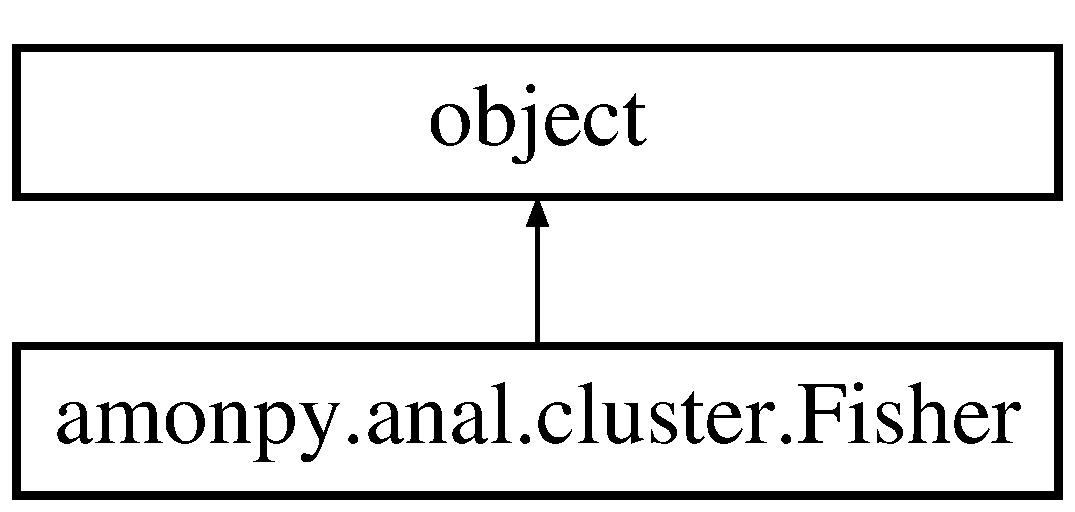
\includegraphics[height=2.000000cm]{df/d03/classamonpy_1_1anal_1_1cluster_1_1_fisher}
\end{center}
\end{figure}
\subsection*{Public Member Functions}
\begin{DoxyCompactItemize}
\item 
def \hyperlink{classamonpy_1_1anal_1_1cluster_1_1_fisher_a1e13053a9daa25129c9c2090b2834434}{\-\_\-\-\_\-init\-\_\-\-\_\-}
\item 
def \hyperlink{classamonpy_1_1anal_1_1cluster_1_1_fisher_a238e5334a3a13208ebeac508dedc55ff}{\-\_\-\-\_\-del\-\_\-\-\_\-}
\item 
def \hyperlink{classamonpy_1_1anal_1_1cluster_1_1_fisher_add8460bfd7a9fa30956eee8248ccff99}{x1}
\item 
def \hyperlink{classamonpy_1_1anal_1_1cluster_1_1_fisher_a1865f423eaf9db7e167962310c3bf72c}{x2}
\item 
def \hyperlink{classamonpy_1_1anal_1_1cluster_1_1_fisher_ab95d705b923546dc9977d8171b6eab49}{cospsi}
\item 
def \hyperlink{classamonpy_1_1anal_1_1cluster_1_1_fisher_a685cc6a7da95f2d37d5aac4eea88e244}{psi}
\item 
def \hyperlink{classamonpy_1_1anal_1_1cluster_1_1_fisher_ac3ecfdabbf304533940d63c1af93de8f}{sigma\-Q}
\item 
def \hyperlink{classamonpy_1_1anal_1_1cluster_1_1_fisher_ab42c5b1d33517dacb0f4885607873780}{sigma\-W}
\item 
def \hyperlink{classamonpy_1_1anal_1_1cluster_1_1_fisher_aaaec3b4e68a97b73d359858cdd11ad65}{Nsigma}
\item 
def \hyperlink{classamonpy_1_1anal_1_1cluster_1_1_fisher_a20eff95eb8d36f153875752a81fcadbc}{x0}
\item 
def \hyperlink{classamonpy_1_1anal_1_1cluster_1_1_fisher_a8f261458556cf374fb773fe17950610d}{radec0}
\item 
def \hyperlink{classamonpy_1_1anal_1_1cluster_1_1_fisher_aa91ec0a66f3d15037cc2e9c4fe51e258}{ra0}
\item 
def \hyperlink{classamonpy_1_1anal_1_1cluster_1_1_fisher_a60cc5f63c12c34f67e51de2dbf7b1ad2}{dec0}
\item 
def \hyperlink{classamonpy_1_1anal_1_1cluster_1_1_fisher_a0818967bb958e432d500365356f25754}{psi1}
\item 
def \hyperlink{classamonpy_1_1anal_1_1cluster_1_1_fisher_aec59ac332e02859dcc3e55e177ca6735}{psi2}
\end{DoxyCompactItemize}
\subsection*{Public Attributes}
\begin{DoxyCompactItemize}
\item 
\hyperlink{classamonpy_1_1anal_1_1cluster_1_1_fisher_a38c295960480aaacc74561dc8f9ef2af}{ev1}
\item 
\hyperlink{classamonpy_1_1anal_1_1cluster_1_1_fisher_ab2cce79b453ffcfced2266553ea60d19}{ev2}
\end{DoxyCompactItemize}
\subsection*{Static Public Attributes}
\begin{DoxyCompactItemize}
\item 
int \hyperlink{classamonpy_1_1anal_1_1cluster_1_1_fisher_a2c44a65df3f24bc786522df8d5aa2db7}{num} = 0
\end{DoxyCompactItemize}


\subsection{Detailed Description}
Analysis class object that uses the \hyperlink{classamonpy_1_1anal_1_1cluster_1_1_fisher}{Fisher} P\-S\-F In particular, the \hyperlink{classamonpy_1_1anal_1_1cluster_1_1_fisher}{Fisher} P\-S\-F is axially symmetric with a single parameter sigma. 

The small angle limit of \hyperlink{classamonpy_1_1anal_1_1cluster_1_1_fisher}{Fisher} gives the 2\-D Gaussian on the plane.

Current version of the code only tests for clustering of pairs of events, but can be generalized in the future.

Inputs\-: ev1, ev2 (a pair of event class objects)

Instances of the \hyperlink{classamonpy_1_1anal_1_1cluster_1_1_fisher}{Fisher} class contain methods that are useful for interpretting the relative position on the two event. 

Definition at line 30 of file cluster.\-py.



\subsection{Constructor \& Destructor Documentation}
\hypertarget{classamonpy_1_1anal_1_1cluster_1_1_fisher_a1e13053a9daa25129c9c2090b2834434}{\index{amonpy\-::anal\-::cluster\-::\-Fisher@{amonpy\-::anal\-::cluster\-::\-Fisher}!\-\_\-\-\_\-init\-\_\-\-\_\-@{\-\_\-\-\_\-init\-\_\-\-\_\-}}
\index{\-\_\-\-\_\-init\-\_\-\-\_\-@{\-\_\-\-\_\-init\-\_\-\-\_\-}!amonpy::anal::cluster::Fisher@{amonpy\-::anal\-::cluster\-::\-Fisher}}
\subsubsection[{\-\_\-\-\_\-init\-\_\-\-\_\-}]{\setlength{\rightskip}{0pt plus 5cm}def amonpy.\-anal.\-cluster.\-Fisher.\-\_\-\-\_\-init\-\_\-\-\_\- (
\begin{DoxyParamCaption}
\item[{}]{self, }
\item[{}]{ev1, }
\item[{}]{ev2}
\end{DoxyParamCaption}
)}}\label{classamonpy_1_1anal_1_1cluster_1_1_fisher_a1e13053a9daa25129c9c2090b2834434}


Definition at line 32 of file cluster.\-py.

\hypertarget{classamonpy_1_1anal_1_1cluster_1_1_fisher_a238e5334a3a13208ebeac508dedc55ff}{\index{amonpy\-::anal\-::cluster\-::\-Fisher@{amonpy\-::anal\-::cluster\-::\-Fisher}!\-\_\-\-\_\-del\-\_\-\-\_\-@{\-\_\-\-\_\-del\-\_\-\-\_\-}}
\index{\-\_\-\-\_\-del\-\_\-\-\_\-@{\-\_\-\-\_\-del\-\_\-\-\_\-}!amonpy::anal::cluster::Fisher@{amonpy\-::anal\-::cluster\-::\-Fisher}}
\subsubsection[{\-\_\-\-\_\-del\-\_\-\-\_\-}]{\setlength{\rightskip}{0pt plus 5cm}def amonpy.\-anal.\-cluster.\-Fisher.\-\_\-\-\_\-del\-\_\-\-\_\- (
\begin{DoxyParamCaption}
\item[{}]{self}
\end{DoxyParamCaption}
)}}\label{classamonpy_1_1anal_1_1cluster_1_1_fisher_a238e5334a3a13208ebeac508dedc55ff}


Definition at line 36 of file cluster.\-py.



\subsection{Member Function Documentation}
\hypertarget{classamonpy_1_1anal_1_1cluster_1_1_fisher_ab95d705b923546dc9977d8171b6eab49}{\index{amonpy\-::anal\-::cluster\-::\-Fisher@{amonpy\-::anal\-::cluster\-::\-Fisher}!cospsi@{cospsi}}
\index{cospsi@{cospsi}!amonpy::anal::cluster::Fisher@{amonpy\-::anal\-::cluster\-::\-Fisher}}
\subsubsection[{cospsi}]{\setlength{\rightskip}{0pt plus 5cm}def amonpy.\-anal.\-cluster.\-Fisher.\-cospsi (
\begin{DoxyParamCaption}
\item[{}]{self}
\end{DoxyParamCaption}
)}}\label{classamonpy_1_1anal_1_1cluster_1_1_fisher_ab95d705b923546dc9977d8171b6eab49}


Definition at line 49 of file cluster.\-py.

\hypertarget{classamonpy_1_1anal_1_1cluster_1_1_fisher_a60cc5f63c12c34f67e51de2dbf7b1ad2}{\index{amonpy\-::anal\-::cluster\-::\-Fisher@{amonpy\-::anal\-::cluster\-::\-Fisher}!dec0@{dec0}}
\index{dec0@{dec0}!amonpy::anal::cluster::Fisher@{amonpy\-::anal\-::cluster\-::\-Fisher}}
\subsubsection[{dec0}]{\setlength{\rightskip}{0pt plus 5cm}def amonpy.\-anal.\-cluster.\-Fisher.\-dec0 (
\begin{DoxyParamCaption}
\item[{}]{self}
\end{DoxyParamCaption}
)}}\label{classamonpy_1_1anal_1_1cluster_1_1_fisher_a60cc5f63c12c34f67e51de2dbf7b1ad2}


Definition at line 82 of file cluster.\-py.

\hypertarget{classamonpy_1_1anal_1_1cluster_1_1_fisher_aaaec3b4e68a97b73d359858cdd11ad65}{\index{amonpy\-::anal\-::cluster\-::\-Fisher@{amonpy\-::anal\-::cluster\-::\-Fisher}!Nsigma@{Nsigma}}
\index{Nsigma@{Nsigma}!amonpy::anal::cluster::Fisher@{amonpy\-::anal\-::cluster\-::\-Fisher}}
\subsubsection[{Nsigma}]{\setlength{\rightskip}{0pt plus 5cm}def amonpy.\-anal.\-cluster.\-Fisher.\-Nsigma (
\begin{DoxyParamCaption}
\item[{}]{self}
\end{DoxyParamCaption}
)}}\label{classamonpy_1_1anal_1_1cluster_1_1_fisher_aaaec3b4e68a97b73d359858cdd11ad65}


Definition at line 65 of file cluster.\-py.

\hypertarget{classamonpy_1_1anal_1_1cluster_1_1_fisher_a685cc6a7da95f2d37d5aac4eea88e244}{\index{amonpy\-::anal\-::cluster\-::\-Fisher@{amonpy\-::anal\-::cluster\-::\-Fisher}!psi@{psi}}
\index{psi@{psi}!amonpy::anal::cluster::Fisher@{amonpy\-::anal\-::cluster\-::\-Fisher}}
\subsubsection[{psi}]{\setlength{\rightskip}{0pt plus 5cm}def amonpy.\-anal.\-cluster.\-Fisher.\-psi (
\begin{DoxyParamCaption}
\item[{}]{self}
\end{DoxyParamCaption}
)}}\label{classamonpy_1_1anal_1_1cluster_1_1_fisher_a685cc6a7da95f2d37d5aac4eea88e244}


Definition at line 53 of file cluster.\-py.

\hypertarget{classamonpy_1_1anal_1_1cluster_1_1_fisher_a0818967bb958e432d500365356f25754}{\index{amonpy\-::anal\-::cluster\-::\-Fisher@{amonpy\-::anal\-::cluster\-::\-Fisher}!psi1@{psi1}}
\index{psi1@{psi1}!amonpy::anal::cluster::Fisher@{amonpy\-::anal\-::cluster\-::\-Fisher}}
\subsubsection[{psi1}]{\setlength{\rightskip}{0pt plus 5cm}def amonpy.\-anal.\-cluster.\-Fisher.\-psi1 (
\begin{DoxyParamCaption}
\item[{}]{self}
\end{DoxyParamCaption}
)}}\label{classamonpy_1_1anal_1_1cluster_1_1_fisher_a0818967bb958e432d500365356f25754}


Definition at line 86 of file cluster.\-py.

\hypertarget{classamonpy_1_1anal_1_1cluster_1_1_fisher_aec59ac332e02859dcc3e55e177ca6735}{\index{amonpy\-::anal\-::cluster\-::\-Fisher@{amonpy\-::anal\-::cluster\-::\-Fisher}!psi2@{psi2}}
\index{psi2@{psi2}!amonpy::anal::cluster::Fisher@{amonpy\-::anal\-::cluster\-::\-Fisher}}
\subsubsection[{psi2}]{\setlength{\rightskip}{0pt plus 5cm}def amonpy.\-anal.\-cluster.\-Fisher.\-psi2 (
\begin{DoxyParamCaption}
\item[{}]{self}
\end{DoxyParamCaption}
)}}\label{classamonpy_1_1anal_1_1cluster_1_1_fisher_aec59ac332e02859dcc3e55e177ca6735}


Definition at line 96 of file cluster.\-py.

\hypertarget{classamonpy_1_1anal_1_1cluster_1_1_fisher_aa91ec0a66f3d15037cc2e9c4fe51e258}{\index{amonpy\-::anal\-::cluster\-::\-Fisher@{amonpy\-::anal\-::cluster\-::\-Fisher}!ra0@{ra0}}
\index{ra0@{ra0}!amonpy::anal::cluster::Fisher@{amonpy\-::anal\-::cluster\-::\-Fisher}}
\subsubsection[{ra0}]{\setlength{\rightskip}{0pt plus 5cm}def amonpy.\-anal.\-cluster.\-Fisher.\-ra0 (
\begin{DoxyParamCaption}
\item[{}]{self}
\end{DoxyParamCaption}
)}}\label{classamonpy_1_1anal_1_1cluster_1_1_fisher_aa91ec0a66f3d15037cc2e9c4fe51e258}


Definition at line 79 of file cluster.\-py.

\hypertarget{classamonpy_1_1anal_1_1cluster_1_1_fisher_a8f261458556cf374fb773fe17950610d}{\index{amonpy\-::anal\-::cluster\-::\-Fisher@{amonpy\-::anal\-::cluster\-::\-Fisher}!radec0@{radec0}}
\index{radec0@{radec0}!amonpy::anal::cluster::Fisher@{amonpy\-::anal\-::cluster\-::\-Fisher}}
\subsubsection[{radec0}]{\setlength{\rightskip}{0pt plus 5cm}def amonpy.\-anal.\-cluster.\-Fisher.\-radec0 (
\begin{DoxyParamCaption}
\item[{}]{self}
\end{DoxyParamCaption}
)}}\label{classamonpy_1_1anal_1_1cluster_1_1_fisher_a8f261458556cf374fb773fe17950610d}


Definition at line 76 of file cluster.\-py.

\hypertarget{classamonpy_1_1anal_1_1cluster_1_1_fisher_ac3ecfdabbf304533940d63c1af93de8f}{\index{amonpy\-::anal\-::cluster\-::\-Fisher@{amonpy\-::anal\-::cluster\-::\-Fisher}!sigma\-Q@{sigma\-Q}}
\index{sigma\-Q@{sigma\-Q}!amonpy::anal::cluster::Fisher@{amonpy\-::anal\-::cluster\-::\-Fisher}}
\subsubsection[{sigma\-Q}]{\setlength{\rightskip}{0pt plus 5cm}def amonpy.\-anal.\-cluster.\-Fisher.\-sigma\-Q (
\begin{DoxyParamCaption}
\item[{}]{self}
\end{DoxyParamCaption}
)}}\label{classamonpy_1_1anal_1_1cluster_1_1_fisher_ac3ecfdabbf304533940d63c1af93de8f}


Definition at line 57 of file cluster.\-py.

\hypertarget{classamonpy_1_1anal_1_1cluster_1_1_fisher_ab42c5b1d33517dacb0f4885607873780}{\index{amonpy\-::anal\-::cluster\-::\-Fisher@{amonpy\-::anal\-::cluster\-::\-Fisher}!sigma\-W@{sigma\-W}}
\index{sigma\-W@{sigma\-W}!amonpy::anal::cluster::Fisher@{amonpy\-::anal\-::cluster\-::\-Fisher}}
\subsubsection[{sigma\-W}]{\setlength{\rightskip}{0pt plus 5cm}def amonpy.\-anal.\-cluster.\-Fisher.\-sigma\-W (
\begin{DoxyParamCaption}
\item[{}]{self}
\end{DoxyParamCaption}
)}}\label{classamonpy_1_1anal_1_1cluster_1_1_fisher_ab42c5b1d33517dacb0f4885607873780}


Definition at line 61 of file cluster.\-py.

\hypertarget{classamonpy_1_1anal_1_1cluster_1_1_fisher_a20eff95eb8d36f153875752a81fcadbc}{\index{amonpy\-::anal\-::cluster\-::\-Fisher@{amonpy\-::anal\-::cluster\-::\-Fisher}!x0@{x0}}
\index{x0@{x0}!amonpy::anal::cluster::Fisher@{amonpy\-::anal\-::cluster\-::\-Fisher}}
\subsubsection[{x0}]{\setlength{\rightskip}{0pt plus 5cm}def amonpy.\-anal.\-cluster.\-Fisher.\-x0 (
\begin{DoxyParamCaption}
\item[{}]{self}
\end{DoxyParamCaption}
)}}\label{classamonpy_1_1anal_1_1cluster_1_1_fisher_a20eff95eb8d36f153875752a81fcadbc}


Definition at line 70 of file cluster.\-py.

\hypertarget{classamonpy_1_1anal_1_1cluster_1_1_fisher_add8460bfd7a9fa30956eee8248ccff99}{\index{amonpy\-::anal\-::cluster\-::\-Fisher@{amonpy\-::anal\-::cluster\-::\-Fisher}!x1@{x1}}
\index{x1@{x1}!amonpy::anal::cluster::Fisher@{amonpy\-::anal\-::cluster\-::\-Fisher}}
\subsubsection[{x1}]{\setlength{\rightskip}{0pt plus 5cm}def amonpy.\-anal.\-cluster.\-Fisher.\-x1 (
\begin{DoxyParamCaption}
\item[{}]{self}
\end{DoxyParamCaption}
)}}\label{classamonpy_1_1anal_1_1cluster_1_1_fisher_add8460bfd7a9fa30956eee8248ccff99}


Definition at line 41 of file cluster.\-py.

\hypertarget{classamonpy_1_1anal_1_1cluster_1_1_fisher_a1865f423eaf9db7e167962310c3bf72c}{\index{amonpy\-::anal\-::cluster\-::\-Fisher@{amonpy\-::anal\-::cluster\-::\-Fisher}!x2@{x2}}
\index{x2@{x2}!amonpy::anal::cluster::Fisher@{amonpy\-::anal\-::cluster\-::\-Fisher}}
\subsubsection[{x2}]{\setlength{\rightskip}{0pt plus 5cm}def amonpy.\-anal.\-cluster.\-Fisher.\-x2 (
\begin{DoxyParamCaption}
\item[{}]{self}
\end{DoxyParamCaption}
)}}\label{classamonpy_1_1anal_1_1cluster_1_1_fisher_a1865f423eaf9db7e167962310c3bf72c}


Definition at line 45 of file cluster.\-py.



\subsection{Member Data Documentation}
\hypertarget{classamonpy_1_1anal_1_1cluster_1_1_fisher_a38c295960480aaacc74561dc8f9ef2af}{\index{amonpy\-::anal\-::cluster\-::\-Fisher@{amonpy\-::anal\-::cluster\-::\-Fisher}!ev1@{ev1}}
\index{ev1@{ev1}!amonpy::anal::cluster::Fisher@{amonpy\-::anal\-::cluster\-::\-Fisher}}
\subsubsection[{ev1}]{\setlength{\rightskip}{0pt plus 5cm}amonpy.\-anal.\-cluster.\-Fisher.\-ev1}}\label{classamonpy_1_1anal_1_1cluster_1_1_fisher_a38c295960480aaacc74561dc8f9ef2af}


Definition at line 34 of file cluster.\-py.

\hypertarget{classamonpy_1_1anal_1_1cluster_1_1_fisher_ab2cce79b453ffcfced2266553ea60d19}{\index{amonpy\-::anal\-::cluster\-::\-Fisher@{amonpy\-::anal\-::cluster\-::\-Fisher}!ev2@{ev2}}
\index{ev2@{ev2}!amonpy::anal::cluster::Fisher@{amonpy\-::anal\-::cluster\-::\-Fisher}}
\subsubsection[{ev2}]{\setlength{\rightskip}{0pt plus 5cm}amonpy.\-anal.\-cluster.\-Fisher.\-ev2}}\label{classamonpy_1_1anal_1_1cluster_1_1_fisher_ab2cce79b453ffcfced2266553ea60d19}


Definition at line 35 of file cluster.\-py.

\hypertarget{classamonpy_1_1anal_1_1cluster_1_1_fisher_a2c44a65df3f24bc786522df8d5aa2db7}{\index{amonpy\-::anal\-::cluster\-::\-Fisher@{amonpy\-::anal\-::cluster\-::\-Fisher}!num@{num}}
\index{num@{num}!amonpy::anal::cluster::Fisher@{amonpy\-::anal\-::cluster\-::\-Fisher}}
\subsubsection[{num}]{\setlength{\rightskip}{0pt plus 5cm}int amonpy.\-anal.\-cluster.\-Fisher.\-num = 0\hspace{0.3cm}{\ttfamily [static]}}}\label{classamonpy_1_1anal_1_1cluster_1_1_fisher_a2c44a65df3f24bc786522df8d5aa2db7}


Definition at line 31 of file cluster.\-py.



The documentation for this class was generated from the following file\-:\begin{DoxyCompactItemize}
\item 
amonpy/anal/\hyperlink{cluster_8py}{cluster.\-py}\end{DoxyCompactItemize}

\hypertarget{classamonpy_1_1anal_1_1cluster_1_1_fisher__tp}{\section{amonpy.\-anal.\-cluster.\-Fisher\-\_\-tp Class Reference}
\label{classamonpy_1_1anal_1_1cluster_1_1_fisher__tp}\index{amonpy.\-anal.\-cluster.\-Fisher\-\_\-tp@{amonpy.\-anal.\-cluster.\-Fisher\-\_\-tp}}
}


Analysis class object that uses the \hyperlink{classamonpy_1_1anal_1_1cluster_1_1_fisher}{Fisher} P\-S\-F In particular, the \hyperlink{classamonpy_1_1anal_1_1cluster_1_1_fisher}{Fisher} P\-S\-F is axially symmetric with a single parameter sigma.  


Inheritance diagram for amonpy.\-anal.\-cluster.\-Fisher\-\_\-tp\-:\begin{figure}[H]
\begin{center}
\leavevmode
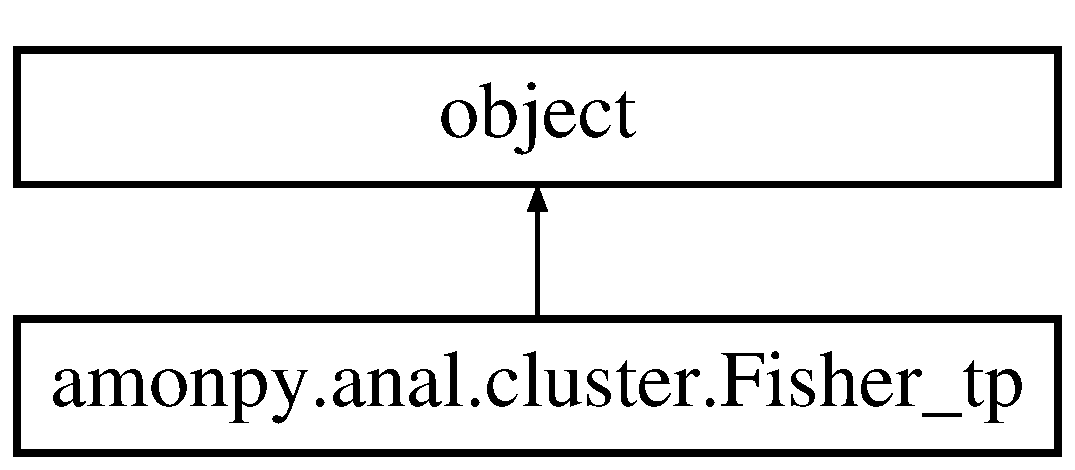
\includegraphics[height=2.000000cm]{d4/ddb/classamonpy_1_1anal_1_1cluster_1_1_fisher__tp}
\end{center}
\end{figure}
\subsection*{Public Member Functions}
\begin{DoxyCompactItemize}
\item 
def \hyperlink{classamonpy_1_1anal_1_1cluster_1_1_fisher__tp_a0baaa3ae5832347d6c4effe3228d1070}{\-\_\-\-\_\-init\-\_\-\-\_\-}
\item 
def \hyperlink{classamonpy_1_1anal_1_1cluster_1_1_fisher__tp_ad550db1bd226069fb26449257c251213}{\-\_\-\-\_\-del\-\_\-\-\_\-}
\item 
def \hyperlink{classamonpy_1_1anal_1_1cluster_1_1_fisher__tp_a88759ac9f5b8f557a1fc65edda6b1865}{x1}
\item 
def \hyperlink{classamonpy_1_1anal_1_1cluster_1_1_fisher__tp_aede64eea0d9a6ea397fc9943442d9534}{x2}
\item 
def \hyperlink{classamonpy_1_1anal_1_1cluster_1_1_fisher__tp_a1429e25626d425974297039b56697d19}{x3}
\item 
def \hyperlink{classamonpy_1_1anal_1_1cluster_1_1_fisher__tp_a0c11d7d64547a5b4c531d192f71d37e3}{cospsi}
\item 
def \hyperlink{classamonpy_1_1anal_1_1cluster_1_1_fisher__tp_a689d0511cf0145cb3126ef3ea70583b2}{cospsi\-\_\-2}
\item 
def \hyperlink{classamonpy_1_1anal_1_1cluster_1_1_fisher__tp_a3af3748863df70d1014ea9bab2e095b2}{cospsi\-\_\-3}
\item 
def \hyperlink{classamonpy_1_1anal_1_1cluster_1_1_fisher__tp_a8f2e659c53f1d1615c2f10d3c8cd6fb3}{psi}
\item 
def \hyperlink{classamonpy_1_1anal_1_1cluster_1_1_fisher__tp_a450b172488a85a08c389a9d2451ed193}{psi\-\_\-2}
\item 
def \hyperlink{classamonpy_1_1anal_1_1cluster_1_1_fisher__tp_a55ac28f856fc291a16f49d816003b773}{psi\-\_\-3}
\item 
def \hyperlink{classamonpy_1_1anal_1_1cluster_1_1_fisher__tp_a51ee7891b489762cd04fdab179870082}{sigma\-Q}
\item 
def \hyperlink{classamonpy_1_1anal_1_1cluster_1_1_fisher__tp_a4c46321795fc93fee607a0cc4d515b7e}{sigma\-W}
\item 
def \hyperlink{classamonpy_1_1anal_1_1cluster_1_1_fisher__tp_a6153df9576e310a26a20e7614c8bccaf}{Nsigma}
\item 
def \hyperlink{classamonpy_1_1anal_1_1cluster_1_1_fisher__tp_adf7afbc7eb930de4db1b7cd182c9f7ec}{Nsigma\-\_\-2}
\item 
def \hyperlink{classamonpy_1_1anal_1_1cluster_1_1_fisher__tp_ae0f081a73cd37010cb67adad216a897b}{Nsigma\-\_\-3}
\item 
def \hyperlink{classamonpy_1_1anal_1_1cluster_1_1_fisher__tp_a604d04ddafd3c54e9ad325adb5e2556b}{x0}
\item 
def \hyperlink{classamonpy_1_1anal_1_1cluster_1_1_fisher__tp_a42d446196e564fc5317470a06cfbba06}{radec0}
\item 
def \hyperlink{classamonpy_1_1anal_1_1cluster_1_1_fisher__tp_a6fd4dc5594118f856b0b92f300168c29}{ra0}
\item 
def \hyperlink{classamonpy_1_1anal_1_1cluster_1_1_fisher__tp_a53495bcf6ab1da20791abc5995e91b80}{dec0}
\item 
def \hyperlink{classamonpy_1_1anal_1_1cluster_1_1_fisher__tp_a3c0bdae70739eb63d804b83bd45cebf2}{psi1}
\item 
def \hyperlink{classamonpy_1_1anal_1_1cluster_1_1_fisher__tp_af15569d830935e813e16a0a073de023a}{psi2}
\item 
def \hyperlink{classamonpy_1_1anal_1_1cluster_1_1_fisher__tp_a2e521151db6f513eeaa52c62f3ae2657}{psi3}
\end{DoxyCompactItemize}
\subsection*{Public Attributes}
\begin{DoxyCompactItemize}
\item 
\hyperlink{classamonpy_1_1anal_1_1cluster_1_1_fisher__tp_a4b282e58dde2fdfc1c815e6f6d2fba5f}{ev1}
\item 
\hyperlink{classamonpy_1_1anal_1_1cluster_1_1_fisher__tp_a5aad4ba062a0103b45387fea062e00f9}{ev2}
\item 
\hyperlink{classamonpy_1_1anal_1_1cluster_1_1_fisher__tp_a222ee1411c4db3f384af8421292f2ec1}{ev3}
\end{DoxyCompactItemize}
\subsection*{Static Public Attributes}
\begin{DoxyCompactItemize}
\item 
int \hyperlink{classamonpy_1_1anal_1_1cluster_1_1_fisher__tp_a3eff8425c58f4b61a8bff758141bfc3e}{num} = 0
\end{DoxyCompactItemize}


\subsection{Detailed Description}
Analysis class object that uses the \hyperlink{classamonpy_1_1anal_1_1cluster_1_1_fisher}{Fisher} P\-S\-F In particular, the \hyperlink{classamonpy_1_1anal_1_1cluster_1_1_fisher}{Fisher} P\-S\-F is axially symmetric with a single parameter sigma. 

The small angle limit of \hyperlink{classamonpy_1_1anal_1_1cluster_1_1_fisher}{Fisher} gives the 2\-D Gaussian on the plane.

Current version of the code only tests for clustering of pairs of events, but can be generalized in the future.

Inputs\-: ev1, ev2, ev3 (a triplet of event class objects)

Instances of the \hyperlink{classamonpy_1_1anal_1_1cluster_1_1_fisher}{Fisher} class contain methods that are useful for interpretting the relative position on the two event. 

Definition at line 110 of file cluster.\-py.



\subsection{Constructor \& Destructor Documentation}
\hypertarget{classamonpy_1_1anal_1_1cluster_1_1_fisher__tp_a0baaa3ae5832347d6c4effe3228d1070}{\index{amonpy\-::anal\-::cluster\-::\-Fisher\-\_\-tp@{amonpy\-::anal\-::cluster\-::\-Fisher\-\_\-tp}!\-\_\-\-\_\-init\-\_\-\-\_\-@{\-\_\-\-\_\-init\-\_\-\-\_\-}}
\index{\-\_\-\-\_\-init\-\_\-\-\_\-@{\-\_\-\-\_\-init\-\_\-\-\_\-}!amonpy::anal::cluster::Fisher_tp@{amonpy\-::anal\-::cluster\-::\-Fisher\-\_\-tp}}
\subsubsection[{\-\_\-\-\_\-init\-\_\-\-\_\-}]{\setlength{\rightskip}{0pt plus 5cm}def amonpy.\-anal.\-cluster.\-Fisher\-\_\-tp.\-\_\-\-\_\-init\-\_\-\-\_\- (
\begin{DoxyParamCaption}
\item[{}]{self, }
\item[{}]{ev1, }
\item[{}]{ev2, }
\item[{}]{ev3}
\end{DoxyParamCaption}
)}}\label{classamonpy_1_1anal_1_1cluster_1_1_fisher__tp_a0baaa3ae5832347d6c4effe3228d1070}


Definition at line 112 of file cluster.\-py.

\hypertarget{classamonpy_1_1anal_1_1cluster_1_1_fisher__tp_ad550db1bd226069fb26449257c251213}{\index{amonpy\-::anal\-::cluster\-::\-Fisher\-\_\-tp@{amonpy\-::anal\-::cluster\-::\-Fisher\-\_\-tp}!\-\_\-\-\_\-del\-\_\-\-\_\-@{\-\_\-\-\_\-del\-\_\-\-\_\-}}
\index{\-\_\-\-\_\-del\-\_\-\-\_\-@{\-\_\-\-\_\-del\-\_\-\-\_\-}!amonpy::anal::cluster::Fisher_tp@{amonpy\-::anal\-::cluster\-::\-Fisher\-\_\-tp}}
\subsubsection[{\-\_\-\-\_\-del\-\_\-\-\_\-}]{\setlength{\rightskip}{0pt plus 5cm}def amonpy.\-anal.\-cluster.\-Fisher\-\_\-tp.\-\_\-\-\_\-del\-\_\-\-\_\- (
\begin{DoxyParamCaption}
\item[{}]{self}
\end{DoxyParamCaption}
)}}\label{classamonpy_1_1anal_1_1cluster_1_1_fisher__tp_ad550db1bd226069fb26449257c251213}


Definition at line 117 of file cluster.\-py.



\subsection{Member Function Documentation}
\hypertarget{classamonpy_1_1anal_1_1cluster_1_1_fisher__tp_a0c11d7d64547a5b4c531d192f71d37e3}{\index{amonpy\-::anal\-::cluster\-::\-Fisher\-\_\-tp@{amonpy\-::anal\-::cluster\-::\-Fisher\-\_\-tp}!cospsi@{cospsi}}
\index{cospsi@{cospsi}!amonpy::anal::cluster::Fisher_tp@{amonpy\-::anal\-::cluster\-::\-Fisher\-\_\-tp}}
\subsubsection[{cospsi}]{\setlength{\rightskip}{0pt plus 5cm}def amonpy.\-anal.\-cluster.\-Fisher\-\_\-tp.\-cospsi (
\begin{DoxyParamCaption}
\item[{}]{self}
\end{DoxyParamCaption}
)}}\label{classamonpy_1_1anal_1_1cluster_1_1_fisher__tp_a0c11d7d64547a5b4c531d192f71d37e3}


Definition at line 134 of file cluster.\-py.

\hypertarget{classamonpy_1_1anal_1_1cluster_1_1_fisher__tp_a689d0511cf0145cb3126ef3ea70583b2}{\index{amonpy\-::anal\-::cluster\-::\-Fisher\-\_\-tp@{amonpy\-::anal\-::cluster\-::\-Fisher\-\_\-tp}!cospsi\-\_\-2@{cospsi\-\_\-2}}
\index{cospsi\-\_\-2@{cospsi\-\_\-2}!amonpy::anal::cluster::Fisher_tp@{amonpy\-::anal\-::cluster\-::\-Fisher\-\_\-tp}}
\subsubsection[{cospsi\-\_\-2}]{\setlength{\rightskip}{0pt plus 5cm}def amonpy.\-anal.\-cluster.\-Fisher\-\_\-tp.\-cospsi\-\_\-2 (
\begin{DoxyParamCaption}
\item[{}]{self}
\end{DoxyParamCaption}
)}}\label{classamonpy_1_1anal_1_1cluster_1_1_fisher__tp_a689d0511cf0145cb3126ef3ea70583b2}


Definition at line 138 of file cluster.\-py.

\hypertarget{classamonpy_1_1anal_1_1cluster_1_1_fisher__tp_a3af3748863df70d1014ea9bab2e095b2}{\index{amonpy\-::anal\-::cluster\-::\-Fisher\-\_\-tp@{amonpy\-::anal\-::cluster\-::\-Fisher\-\_\-tp}!cospsi\-\_\-3@{cospsi\-\_\-3}}
\index{cospsi\-\_\-3@{cospsi\-\_\-3}!amonpy::anal::cluster::Fisher_tp@{amonpy\-::anal\-::cluster\-::\-Fisher\-\_\-tp}}
\subsubsection[{cospsi\-\_\-3}]{\setlength{\rightskip}{0pt plus 5cm}def amonpy.\-anal.\-cluster.\-Fisher\-\_\-tp.\-cospsi\-\_\-3 (
\begin{DoxyParamCaption}
\item[{}]{self}
\end{DoxyParamCaption}
)}}\label{classamonpy_1_1anal_1_1cluster_1_1_fisher__tp_a3af3748863df70d1014ea9bab2e095b2}


Definition at line 142 of file cluster.\-py.

\hypertarget{classamonpy_1_1anal_1_1cluster_1_1_fisher__tp_a53495bcf6ab1da20791abc5995e91b80}{\index{amonpy\-::anal\-::cluster\-::\-Fisher\-\_\-tp@{amonpy\-::anal\-::cluster\-::\-Fisher\-\_\-tp}!dec0@{dec0}}
\index{dec0@{dec0}!amonpy::anal::cluster::Fisher_tp@{amonpy\-::anal\-::cluster\-::\-Fisher\-\_\-tp}}
\subsubsection[{dec0}]{\setlength{\rightskip}{0pt plus 5cm}def amonpy.\-anal.\-cluster.\-Fisher\-\_\-tp.\-dec0 (
\begin{DoxyParamCaption}
\item[{}]{self}
\end{DoxyParamCaption}
)}}\label{classamonpy_1_1anal_1_1cluster_1_1_fisher__tp_a53495bcf6ab1da20791abc5995e91b80}


Definition at line 194 of file cluster.\-py.

\hypertarget{classamonpy_1_1anal_1_1cluster_1_1_fisher__tp_a6153df9576e310a26a20e7614c8bccaf}{\index{amonpy\-::anal\-::cluster\-::\-Fisher\-\_\-tp@{amonpy\-::anal\-::cluster\-::\-Fisher\-\_\-tp}!Nsigma@{Nsigma}}
\index{Nsigma@{Nsigma}!amonpy::anal::cluster::Fisher_tp@{amonpy\-::anal\-::cluster\-::\-Fisher\-\_\-tp}}
\subsubsection[{Nsigma}]{\setlength{\rightskip}{0pt plus 5cm}def amonpy.\-anal.\-cluster.\-Fisher\-\_\-tp.\-Nsigma (
\begin{DoxyParamCaption}
\item[{}]{self}
\end{DoxyParamCaption}
)}}\label{classamonpy_1_1anal_1_1cluster_1_1_fisher__tp_a6153df9576e310a26a20e7614c8bccaf}


Definition at line 167 of file cluster.\-py.

\hypertarget{classamonpy_1_1anal_1_1cluster_1_1_fisher__tp_adf7afbc7eb930de4db1b7cd182c9f7ec}{\index{amonpy\-::anal\-::cluster\-::\-Fisher\-\_\-tp@{amonpy\-::anal\-::cluster\-::\-Fisher\-\_\-tp}!Nsigma\-\_\-2@{Nsigma\-\_\-2}}
\index{Nsigma\-\_\-2@{Nsigma\-\_\-2}!amonpy::anal::cluster::Fisher_tp@{amonpy\-::anal\-::cluster\-::\-Fisher\-\_\-tp}}
\subsubsection[{Nsigma\-\_\-2}]{\setlength{\rightskip}{0pt plus 5cm}def amonpy.\-anal.\-cluster.\-Fisher\-\_\-tp.\-Nsigma\-\_\-2 (
\begin{DoxyParamCaption}
\item[{}]{self}
\end{DoxyParamCaption}
)}}\label{classamonpy_1_1anal_1_1cluster_1_1_fisher__tp_adf7afbc7eb930de4db1b7cd182c9f7ec}


Definition at line 172 of file cluster.\-py.

\hypertarget{classamonpy_1_1anal_1_1cluster_1_1_fisher__tp_ae0f081a73cd37010cb67adad216a897b}{\index{amonpy\-::anal\-::cluster\-::\-Fisher\-\_\-tp@{amonpy\-::anal\-::cluster\-::\-Fisher\-\_\-tp}!Nsigma\-\_\-3@{Nsigma\-\_\-3}}
\index{Nsigma\-\_\-3@{Nsigma\-\_\-3}!amonpy::anal::cluster::Fisher_tp@{amonpy\-::anal\-::cluster\-::\-Fisher\-\_\-tp}}
\subsubsection[{Nsigma\-\_\-3}]{\setlength{\rightskip}{0pt plus 5cm}def amonpy.\-anal.\-cluster.\-Fisher\-\_\-tp.\-Nsigma\-\_\-3 (
\begin{DoxyParamCaption}
\item[{}]{self}
\end{DoxyParamCaption}
)}}\label{classamonpy_1_1anal_1_1cluster_1_1_fisher__tp_ae0f081a73cd37010cb67adad216a897b}


Definition at line 176 of file cluster.\-py.

\hypertarget{classamonpy_1_1anal_1_1cluster_1_1_fisher__tp_a8f2e659c53f1d1615c2f10d3c8cd6fb3}{\index{amonpy\-::anal\-::cluster\-::\-Fisher\-\_\-tp@{amonpy\-::anal\-::cluster\-::\-Fisher\-\_\-tp}!psi@{psi}}
\index{psi@{psi}!amonpy::anal::cluster::Fisher_tp@{amonpy\-::anal\-::cluster\-::\-Fisher\-\_\-tp}}
\subsubsection[{psi}]{\setlength{\rightskip}{0pt plus 5cm}def amonpy.\-anal.\-cluster.\-Fisher\-\_\-tp.\-psi (
\begin{DoxyParamCaption}
\item[{}]{self}
\end{DoxyParamCaption}
)}}\label{classamonpy_1_1anal_1_1cluster_1_1_fisher__tp_a8f2e659c53f1d1615c2f10d3c8cd6fb3}


Definition at line 146 of file cluster.\-py.

\hypertarget{classamonpy_1_1anal_1_1cluster_1_1_fisher__tp_a3c0bdae70739eb63d804b83bd45cebf2}{\index{amonpy\-::anal\-::cluster\-::\-Fisher\-\_\-tp@{amonpy\-::anal\-::cluster\-::\-Fisher\-\_\-tp}!psi1@{psi1}}
\index{psi1@{psi1}!amonpy::anal::cluster::Fisher_tp@{amonpy\-::anal\-::cluster\-::\-Fisher\-\_\-tp}}
\subsubsection[{psi1}]{\setlength{\rightskip}{0pt plus 5cm}def amonpy.\-anal.\-cluster.\-Fisher\-\_\-tp.\-psi1 (
\begin{DoxyParamCaption}
\item[{}]{self}
\end{DoxyParamCaption}
)}}\label{classamonpy_1_1anal_1_1cluster_1_1_fisher__tp_a3c0bdae70739eb63d804b83bd45cebf2}


Definition at line 198 of file cluster.\-py.

\hypertarget{classamonpy_1_1anal_1_1cluster_1_1_fisher__tp_af15569d830935e813e16a0a073de023a}{\index{amonpy\-::anal\-::cluster\-::\-Fisher\-\_\-tp@{amonpy\-::anal\-::cluster\-::\-Fisher\-\_\-tp}!psi2@{psi2}}
\index{psi2@{psi2}!amonpy::anal::cluster::Fisher_tp@{amonpy\-::anal\-::cluster\-::\-Fisher\-\_\-tp}}
\subsubsection[{psi2}]{\setlength{\rightskip}{0pt plus 5cm}def amonpy.\-anal.\-cluster.\-Fisher\-\_\-tp.\-psi2 (
\begin{DoxyParamCaption}
\item[{}]{self}
\end{DoxyParamCaption}
)}}\label{classamonpy_1_1anal_1_1cluster_1_1_fisher__tp_af15569d830935e813e16a0a073de023a}


Definition at line 203 of file cluster.\-py.

\hypertarget{classamonpy_1_1anal_1_1cluster_1_1_fisher__tp_a2e521151db6f513eeaa52c62f3ae2657}{\index{amonpy\-::anal\-::cluster\-::\-Fisher\-\_\-tp@{amonpy\-::anal\-::cluster\-::\-Fisher\-\_\-tp}!psi3@{psi3}}
\index{psi3@{psi3}!amonpy::anal::cluster::Fisher_tp@{amonpy\-::anal\-::cluster\-::\-Fisher\-\_\-tp}}
\subsubsection[{psi3}]{\setlength{\rightskip}{0pt plus 5cm}def amonpy.\-anal.\-cluster.\-Fisher\-\_\-tp.\-psi3 (
\begin{DoxyParamCaption}
\item[{}]{self}
\end{DoxyParamCaption}
)}}\label{classamonpy_1_1anal_1_1cluster_1_1_fisher__tp_a2e521151db6f513eeaa52c62f3ae2657}


Definition at line 208 of file cluster.\-py.

\hypertarget{classamonpy_1_1anal_1_1cluster_1_1_fisher__tp_a450b172488a85a08c389a9d2451ed193}{\index{amonpy\-::anal\-::cluster\-::\-Fisher\-\_\-tp@{amonpy\-::anal\-::cluster\-::\-Fisher\-\_\-tp}!psi\-\_\-2@{psi\-\_\-2}}
\index{psi\-\_\-2@{psi\-\_\-2}!amonpy::anal::cluster::Fisher_tp@{amonpy\-::anal\-::cluster\-::\-Fisher\-\_\-tp}}
\subsubsection[{psi\-\_\-2}]{\setlength{\rightskip}{0pt plus 5cm}def amonpy.\-anal.\-cluster.\-Fisher\-\_\-tp.\-psi\-\_\-2 (
\begin{DoxyParamCaption}
\item[{}]{self}
\end{DoxyParamCaption}
)}}\label{classamonpy_1_1anal_1_1cluster_1_1_fisher__tp_a450b172488a85a08c389a9d2451ed193}


Definition at line 150 of file cluster.\-py.

\hypertarget{classamonpy_1_1anal_1_1cluster_1_1_fisher__tp_a55ac28f856fc291a16f49d816003b773}{\index{amonpy\-::anal\-::cluster\-::\-Fisher\-\_\-tp@{amonpy\-::anal\-::cluster\-::\-Fisher\-\_\-tp}!psi\-\_\-3@{psi\-\_\-3}}
\index{psi\-\_\-3@{psi\-\_\-3}!amonpy::anal::cluster::Fisher_tp@{amonpy\-::anal\-::cluster\-::\-Fisher\-\_\-tp}}
\subsubsection[{psi\-\_\-3}]{\setlength{\rightskip}{0pt plus 5cm}def amonpy.\-anal.\-cluster.\-Fisher\-\_\-tp.\-psi\-\_\-3 (
\begin{DoxyParamCaption}
\item[{}]{self}
\end{DoxyParamCaption}
)}}\label{classamonpy_1_1anal_1_1cluster_1_1_fisher__tp_a55ac28f856fc291a16f49d816003b773}


Definition at line 154 of file cluster.\-py.

\hypertarget{classamonpy_1_1anal_1_1cluster_1_1_fisher__tp_a6fd4dc5594118f856b0b92f300168c29}{\index{amonpy\-::anal\-::cluster\-::\-Fisher\-\_\-tp@{amonpy\-::anal\-::cluster\-::\-Fisher\-\_\-tp}!ra0@{ra0}}
\index{ra0@{ra0}!amonpy::anal::cluster::Fisher_tp@{amonpy\-::anal\-::cluster\-::\-Fisher\-\_\-tp}}
\subsubsection[{ra0}]{\setlength{\rightskip}{0pt plus 5cm}def amonpy.\-anal.\-cluster.\-Fisher\-\_\-tp.\-ra0 (
\begin{DoxyParamCaption}
\item[{}]{self}
\end{DoxyParamCaption}
)}}\label{classamonpy_1_1anal_1_1cluster_1_1_fisher__tp_a6fd4dc5594118f856b0b92f300168c29}


Definition at line 191 of file cluster.\-py.

\hypertarget{classamonpy_1_1anal_1_1cluster_1_1_fisher__tp_a42d446196e564fc5317470a06cfbba06}{\index{amonpy\-::anal\-::cluster\-::\-Fisher\-\_\-tp@{amonpy\-::anal\-::cluster\-::\-Fisher\-\_\-tp}!radec0@{radec0}}
\index{radec0@{radec0}!amonpy::anal::cluster::Fisher_tp@{amonpy\-::anal\-::cluster\-::\-Fisher\-\_\-tp}}
\subsubsection[{radec0}]{\setlength{\rightskip}{0pt plus 5cm}def amonpy.\-anal.\-cluster.\-Fisher\-\_\-tp.\-radec0 (
\begin{DoxyParamCaption}
\item[{}]{self}
\end{DoxyParamCaption}
)}}\label{classamonpy_1_1anal_1_1cluster_1_1_fisher__tp_a42d446196e564fc5317470a06cfbba06}


Definition at line 188 of file cluster.\-py.

\hypertarget{classamonpy_1_1anal_1_1cluster_1_1_fisher__tp_a51ee7891b489762cd04fdab179870082}{\index{amonpy\-::anal\-::cluster\-::\-Fisher\-\_\-tp@{amonpy\-::anal\-::cluster\-::\-Fisher\-\_\-tp}!sigma\-Q@{sigma\-Q}}
\index{sigma\-Q@{sigma\-Q}!amonpy::anal::cluster::Fisher_tp@{amonpy\-::anal\-::cluster\-::\-Fisher\-\_\-tp}}
\subsubsection[{sigma\-Q}]{\setlength{\rightskip}{0pt plus 5cm}def amonpy.\-anal.\-cluster.\-Fisher\-\_\-tp.\-sigma\-Q (
\begin{DoxyParamCaption}
\item[{}]{self}
\end{DoxyParamCaption}
)}}\label{classamonpy_1_1anal_1_1cluster_1_1_fisher__tp_a51ee7891b489762cd04fdab179870082}


Definition at line 158 of file cluster.\-py.

\hypertarget{classamonpy_1_1anal_1_1cluster_1_1_fisher__tp_a4c46321795fc93fee607a0cc4d515b7e}{\index{amonpy\-::anal\-::cluster\-::\-Fisher\-\_\-tp@{amonpy\-::anal\-::cluster\-::\-Fisher\-\_\-tp}!sigma\-W@{sigma\-W}}
\index{sigma\-W@{sigma\-W}!amonpy::anal::cluster::Fisher_tp@{amonpy\-::anal\-::cluster\-::\-Fisher\-\_\-tp}}
\subsubsection[{sigma\-W}]{\setlength{\rightskip}{0pt plus 5cm}def amonpy.\-anal.\-cluster.\-Fisher\-\_\-tp.\-sigma\-W (
\begin{DoxyParamCaption}
\item[{}]{self}
\end{DoxyParamCaption}
)}}\label{classamonpy_1_1anal_1_1cluster_1_1_fisher__tp_a4c46321795fc93fee607a0cc4d515b7e}


Definition at line 162 of file cluster.\-py.

\hypertarget{classamonpy_1_1anal_1_1cluster_1_1_fisher__tp_a604d04ddafd3c54e9ad325adb5e2556b}{\index{amonpy\-::anal\-::cluster\-::\-Fisher\-\_\-tp@{amonpy\-::anal\-::cluster\-::\-Fisher\-\_\-tp}!x0@{x0}}
\index{x0@{x0}!amonpy::anal::cluster::Fisher_tp@{amonpy\-::anal\-::cluster\-::\-Fisher\-\_\-tp}}
\subsubsection[{x0}]{\setlength{\rightskip}{0pt plus 5cm}def amonpy.\-anal.\-cluster.\-Fisher\-\_\-tp.\-x0 (
\begin{DoxyParamCaption}
\item[{}]{self}
\end{DoxyParamCaption}
)}}\label{classamonpy_1_1anal_1_1cluster_1_1_fisher__tp_a604d04ddafd3c54e9ad325adb5e2556b}


Definition at line 181 of file cluster.\-py.

\hypertarget{classamonpy_1_1anal_1_1cluster_1_1_fisher__tp_a88759ac9f5b8f557a1fc65edda6b1865}{\index{amonpy\-::anal\-::cluster\-::\-Fisher\-\_\-tp@{amonpy\-::anal\-::cluster\-::\-Fisher\-\_\-tp}!x1@{x1}}
\index{x1@{x1}!amonpy::anal::cluster::Fisher_tp@{amonpy\-::anal\-::cluster\-::\-Fisher\-\_\-tp}}
\subsubsection[{x1}]{\setlength{\rightskip}{0pt plus 5cm}def amonpy.\-anal.\-cluster.\-Fisher\-\_\-tp.\-x1 (
\begin{DoxyParamCaption}
\item[{}]{self}
\end{DoxyParamCaption}
)}}\label{classamonpy_1_1anal_1_1cluster_1_1_fisher__tp_a88759ac9f5b8f557a1fc65edda6b1865}


Definition at line 122 of file cluster.\-py.

\hypertarget{classamonpy_1_1anal_1_1cluster_1_1_fisher__tp_aede64eea0d9a6ea397fc9943442d9534}{\index{amonpy\-::anal\-::cluster\-::\-Fisher\-\_\-tp@{amonpy\-::anal\-::cluster\-::\-Fisher\-\_\-tp}!x2@{x2}}
\index{x2@{x2}!amonpy::anal::cluster::Fisher_tp@{amonpy\-::anal\-::cluster\-::\-Fisher\-\_\-tp}}
\subsubsection[{x2}]{\setlength{\rightskip}{0pt plus 5cm}def amonpy.\-anal.\-cluster.\-Fisher\-\_\-tp.\-x2 (
\begin{DoxyParamCaption}
\item[{}]{self}
\end{DoxyParamCaption}
)}}\label{classamonpy_1_1anal_1_1cluster_1_1_fisher__tp_aede64eea0d9a6ea397fc9943442d9534}


Definition at line 126 of file cluster.\-py.

\hypertarget{classamonpy_1_1anal_1_1cluster_1_1_fisher__tp_a1429e25626d425974297039b56697d19}{\index{amonpy\-::anal\-::cluster\-::\-Fisher\-\_\-tp@{amonpy\-::anal\-::cluster\-::\-Fisher\-\_\-tp}!x3@{x3}}
\index{x3@{x3}!amonpy::anal::cluster::Fisher_tp@{amonpy\-::anal\-::cluster\-::\-Fisher\-\_\-tp}}
\subsubsection[{x3}]{\setlength{\rightskip}{0pt plus 5cm}def amonpy.\-anal.\-cluster.\-Fisher\-\_\-tp.\-x3 (
\begin{DoxyParamCaption}
\item[{}]{self}
\end{DoxyParamCaption}
)}}\label{classamonpy_1_1anal_1_1cluster_1_1_fisher__tp_a1429e25626d425974297039b56697d19}


Definition at line 130 of file cluster.\-py.



\subsection{Member Data Documentation}
\hypertarget{classamonpy_1_1anal_1_1cluster_1_1_fisher__tp_a4b282e58dde2fdfc1c815e6f6d2fba5f}{\index{amonpy\-::anal\-::cluster\-::\-Fisher\-\_\-tp@{amonpy\-::anal\-::cluster\-::\-Fisher\-\_\-tp}!ev1@{ev1}}
\index{ev1@{ev1}!amonpy::anal::cluster::Fisher_tp@{amonpy\-::anal\-::cluster\-::\-Fisher\-\_\-tp}}
\subsubsection[{ev1}]{\setlength{\rightskip}{0pt plus 5cm}amonpy.\-anal.\-cluster.\-Fisher\-\_\-tp.\-ev1}}\label{classamonpy_1_1anal_1_1cluster_1_1_fisher__tp_a4b282e58dde2fdfc1c815e6f6d2fba5f}


Definition at line 114 of file cluster.\-py.

\hypertarget{classamonpy_1_1anal_1_1cluster_1_1_fisher__tp_a5aad4ba062a0103b45387fea062e00f9}{\index{amonpy\-::anal\-::cluster\-::\-Fisher\-\_\-tp@{amonpy\-::anal\-::cluster\-::\-Fisher\-\_\-tp}!ev2@{ev2}}
\index{ev2@{ev2}!amonpy::anal::cluster::Fisher_tp@{amonpy\-::anal\-::cluster\-::\-Fisher\-\_\-tp}}
\subsubsection[{ev2}]{\setlength{\rightskip}{0pt plus 5cm}amonpy.\-anal.\-cluster.\-Fisher\-\_\-tp.\-ev2}}\label{classamonpy_1_1anal_1_1cluster_1_1_fisher__tp_a5aad4ba062a0103b45387fea062e00f9}


Definition at line 115 of file cluster.\-py.

\hypertarget{classamonpy_1_1anal_1_1cluster_1_1_fisher__tp_a222ee1411c4db3f384af8421292f2ec1}{\index{amonpy\-::anal\-::cluster\-::\-Fisher\-\_\-tp@{amonpy\-::anal\-::cluster\-::\-Fisher\-\_\-tp}!ev3@{ev3}}
\index{ev3@{ev3}!amonpy::anal::cluster::Fisher_tp@{amonpy\-::anal\-::cluster\-::\-Fisher\-\_\-tp}}
\subsubsection[{ev3}]{\setlength{\rightskip}{0pt plus 5cm}amonpy.\-anal.\-cluster.\-Fisher\-\_\-tp.\-ev3}}\label{classamonpy_1_1anal_1_1cluster_1_1_fisher__tp_a222ee1411c4db3f384af8421292f2ec1}


Definition at line 116 of file cluster.\-py.

\hypertarget{classamonpy_1_1anal_1_1cluster_1_1_fisher__tp_a3eff8425c58f4b61a8bff758141bfc3e}{\index{amonpy\-::anal\-::cluster\-::\-Fisher\-\_\-tp@{amonpy\-::anal\-::cluster\-::\-Fisher\-\_\-tp}!num@{num}}
\index{num@{num}!amonpy::anal::cluster::Fisher_tp@{amonpy\-::anal\-::cluster\-::\-Fisher\-\_\-tp}}
\subsubsection[{num}]{\setlength{\rightskip}{0pt plus 5cm}int amonpy.\-anal.\-cluster.\-Fisher\-\_\-tp.\-num = 0\hspace{0.3cm}{\ttfamily [static]}}}\label{classamonpy_1_1anal_1_1cluster_1_1_fisher__tp_a3eff8425c58f4b61a8bff758141bfc3e}


Definition at line 111 of file cluster.\-py.



The documentation for this class was generated from the following file\-:\begin{DoxyCompactItemize}
\item 
amonpy/anal/\hyperlink{cluster_8py}{cluster.\-py}\end{DoxyCompactItemize}

\hypertarget{classamonpy_1_1sim_1_1sidereal_1_1_fixed_zone}{\section{amonpy.\-sim.\-sidereal.\-Fixed\-Zone Class Reference}
\label{classamonpy_1_1sim_1_1sidereal_1_1_fixed_zone}\index{amonpy.\-sim.\-sidereal.\-Fixed\-Zone@{amonpy.\-sim.\-sidereal.\-Fixed\-Zone}}
}


Represents a time zone with a fixed offset east of U\-T\-C.  


Inheritance diagram for amonpy.\-sim.\-sidereal.\-Fixed\-Zone\-:\begin{figure}[H]
\begin{center}
\leavevmode
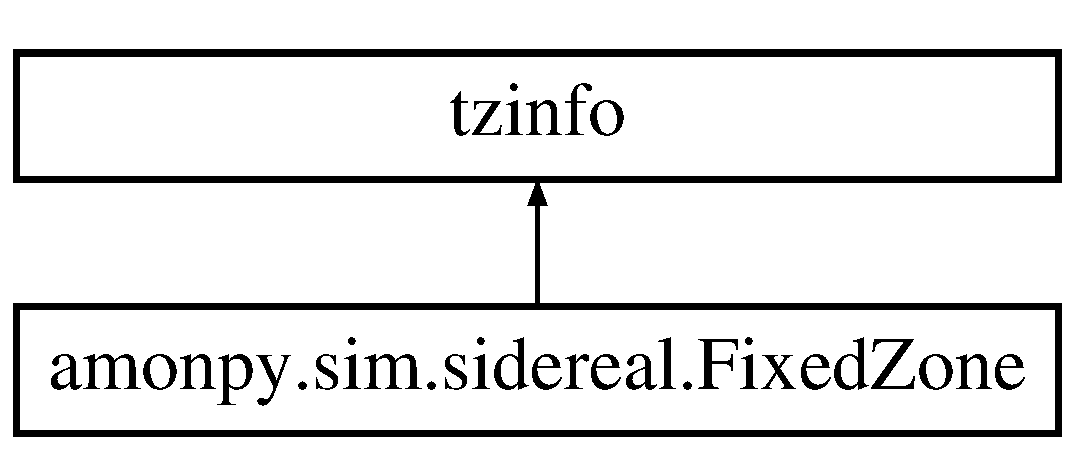
\includegraphics[height=2.000000cm]{d0/d58/classamonpy_1_1sim_1_1sidereal_1_1_fixed_zone}
\end{center}
\end{figure}
\subsection*{Public Member Functions}
\begin{DoxyCompactItemize}
\item 
def \hyperlink{classamonpy_1_1sim_1_1sidereal_1_1_fixed_zone_a4b1001f54b5a79fd3d4e36d22d6b1773}{\-\_\-\-\_\-init\-\_\-\-\_\-}
\begin{DoxyCompactList}\small\item\em Constructor for \hyperlink{classamonpy_1_1sim_1_1sidereal_1_1_fixed_zone}{Fixed\-Zone}. \end{DoxyCompactList}\item 
def \hyperlink{classamonpy_1_1sim_1_1sidereal_1_1_fixed_zone_a259dc7d17941495116721e9ad5aa75a5}{utcoffset}
\begin{DoxyCompactList}\small\item\em Return self's offset east of U\-T\-C. \end{DoxyCompactList}\item 
def \hyperlink{classamonpy_1_1sim_1_1sidereal_1_1_fixed_zone_a71498be1686ee252280e0aab5585c56b}{tzname}
\begin{DoxyCompactList}\small\item\em Return self's name. \end{DoxyCompactList}\item 
def \hyperlink{classamonpy_1_1sim_1_1sidereal_1_1_fixed_zone_a5a37ebf256e2dc3233aaf05c19a2f84d}{dst}
\begin{DoxyCompactList}\small\item\em Return self's daylight time offset. \end{DoxyCompactList}\end{DoxyCompactItemize}


\subsection{Detailed Description}
Represents a time zone with a fixed offset east of U\-T\-C. 

Exports\-: \hyperlink{classamonpy_1_1sim_1_1sidereal_1_1_fixed_zone}{Fixed\-Zone} ( hours, minutes, name )\-: \mbox{[} (hours is a signed offset in hours as an int) and (minutes is a signed offset in minutes as an int) -\/$>$ return a new \hyperlink{classamonpy_1_1sim_1_1sidereal_1_1_fixed_zone}{Fixed\-Zone} instance representing those offsets east of U\-T\-C \mbox{]} State/\-Invariants\-: .\-\_\-\-\_\-offset\-: \mbox{[} a datetime.\-timedelta representing self's offset east of U\-T\-C \mbox{]} .\-\_\-\-\_\-name\-: \mbox{[} as passed to the constructor's name argument \mbox{]} 

Definition at line 387 of file sidereal.\-py.



\subsection{Constructor \& Destructor Documentation}
\hypertarget{classamonpy_1_1sim_1_1sidereal_1_1_fixed_zone_a4b1001f54b5a79fd3d4e36d22d6b1773}{\index{amonpy\-::sim\-::sidereal\-::\-Fixed\-Zone@{amonpy\-::sim\-::sidereal\-::\-Fixed\-Zone}!\-\_\-\-\_\-init\-\_\-\-\_\-@{\-\_\-\-\_\-init\-\_\-\-\_\-}}
\index{\-\_\-\-\_\-init\-\_\-\-\_\-@{\-\_\-\-\_\-init\-\_\-\-\_\-}!amonpy::sim::sidereal::FixedZone@{amonpy\-::sim\-::sidereal\-::\-Fixed\-Zone}}
\subsubsection[{\-\_\-\-\_\-init\-\_\-\-\_\-}]{\setlength{\rightskip}{0pt plus 5cm}def amonpy.\-sim.\-sidereal.\-Fixed\-Zone.\-\_\-\-\_\-init\-\_\-\-\_\- (
\begin{DoxyParamCaption}
\item[{}]{self, }
\item[{}]{hh, }
\item[{}]{mm, }
\item[{}]{name}
\end{DoxyParamCaption}
)}}\label{classamonpy_1_1sim_1_1sidereal_1_1_fixed_zone_a4b1001f54b5a79fd3d4e36d22d6b1773}


Constructor for \hyperlink{classamonpy_1_1sim_1_1sidereal_1_1_fixed_zone}{Fixed\-Zone}. 



Definition at line 391 of file sidereal.\-py.



\subsection{Member Function Documentation}
\hypertarget{classamonpy_1_1sim_1_1sidereal_1_1_fixed_zone_a5a37ebf256e2dc3233aaf05c19a2f84d}{\index{amonpy\-::sim\-::sidereal\-::\-Fixed\-Zone@{amonpy\-::sim\-::sidereal\-::\-Fixed\-Zone}!dst@{dst}}
\index{dst@{dst}!amonpy::sim::sidereal::FixedZone@{amonpy\-::sim\-::sidereal\-::\-Fixed\-Zone}}
\subsubsection[{dst}]{\setlength{\rightskip}{0pt plus 5cm}def amonpy.\-sim.\-sidereal.\-Fixed\-Zone.\-dst (
\begin{DoxyParamCaption}
\item[{}]{self, }
\item[{}]{dt}
\end{DoxyParamCaption}
)}}\label{classamonpy_1_1sim_1_1sidereal_1_1_fixed_zone_a5a37ebf256e2dc3233aaf05c19a2f84d}


Return self's daylight time offset. 



Definition at line 407 of file sidereal.\-py.

\hypertarget{classamonpy_1_1sim_1_1sidereal_1_1_fixed_zone_a71498be1686ee252280e0aab5585c56b}{\index{amonpy\-::sim\-::sidereal\-::\-Fixed\-Zone@{amonpy\-::sim\-::sidereal\-::\-Fixed\-Zone}!tzname@{tzname}}
\index{tzname@{tzname}!amonpy::sim::sidereal::FixedZone@{amonpy\-::sim\-::sidereal\-::\-Fixed\-Zone}}
\subsubsection[{tzname}]{\setlength{\rightskip}{0pt plus 5cm}def amonpy.\-sim.\-sidereal.\-Fixed\-Zone.\-tzname (
\begin{DoxyParamCaption}
\item[{}]{self, }
\item[{}]{dt}
\end{DoxyParamCaption}
)}}\label{classamonpy_1_1sim_1_1sidereal_1_1_fixed_zone_a71498be1686ee252280e0aab5585c56b}


Return self's name. 



Definition at line 402 of file sidereal.\-py.

\hypertarget{classamonpy_1_1sim_1_1sidereal_1_1_fixed_zone_a259dc7d17941495116721e9ad5aa75a5}{\index{amonpy\-::sim\-::sidereal\-::\-Fixed\-Zone@{amonpy\-::sim\-::sidereal\-::\-Fixed\-Zone}!utcoffset@{utcoffset}}
\index{utcoffset@{utcoffset}!amonpy::sim::sidereal::FixedZone@{amonpy\-::sim\-::sidereal\-::\-Fixed\-Zone}}
\subsubsection[{utcoffset}]{\setlength{\rightskip}{0pt plus 5cm}def amonpy.\-sim.\-sidereal.\-Fixed\-Zone.\-utcoffset (
\begin{DoxyParamCaption}
\item[{}]{self, }
\item[{}]{dt}
\end{DoxyParamCaption}
)}}\label{classamonpy_1_1sim_1_1sidereal_1_1_fixed_zone_a259dc7d17941495116721e9ad5aa75a5}


Return self's offset east of U\-T\-C. 



Definition at line 397 of file sidereal.\-py.



The documentation for this class was generated from the following file\-:\begin{DoxyCompactItemize}
\item 
amonpy/sim/\hyperlink{sidereal_8py}{sidereal.\-py}\end{DoxyCompactItemize}

\hypertarget{classamonpy_1_1sim_1_1sidereal__m_1_1_fixed_zone}{\section{amonpy.\-sim.\-sidereal\-\_\-m.\-Fixed\-Zone Class Reference}
\label{classamonpy_1_1sim_1_1sidereal__m_1_1_fixed_zone}\index{amonpy.\-sim.\-sidereal\-\_\-m.\-Fixed\-Zone@{amonpy.\-sim.\-sidereal\-\_\-m.\-Fixed\-Zone}}
}


Represents a time zone with a fixed offset east of U\-T\-C.  


Inheritance diagram for amonpy.\-sim.\-sidereal\-\_\-m.\-Fixed\-Zone\-:\begin{figure}[H]
\begin{center}
\leavevmode
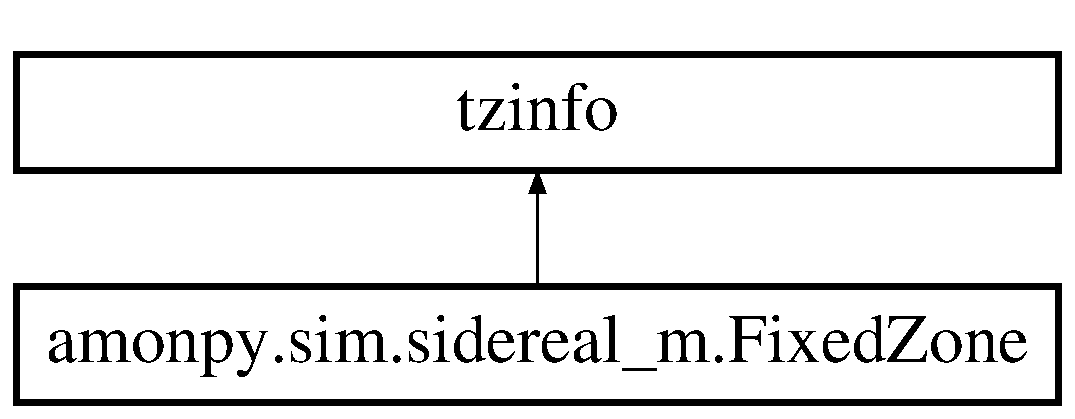
\includegraphics[height=2.000000cm]{d4/d37/classamonpy_1_1sim_1_1sidereal__m_1_1_fixed_zone}
\end{center}
\end{figure}
\subsection*{Public Member Functions}
\begin{DoxyCompactItemize}
\item 
def \hyperlink{classamonpy_1_1sim_1_1sidereal__m_1_1_fixed_zone_a0e29cd625591a8a1bad0c567ad775898}{\-\_\-\-\_\-init\-\_\-\-\_\-}
\begin{DoxyCompactList}\small\item\em Constructor for \hyperlink{classamonpy_1_1sim_1_1sidereal__m_1_1_fixed_zone}{Fixed\-Zone}. \end{DoxyCompactList}\item 
def \hyperlink{classamonpy_1_1sim_1_1sidereal__m_1_1_fixed_zone_a747541b59e840bcfdf7df8805f9b1179}{utcoffset}
\begin{DoxyCompactList}\small\item\em Return self's offset east of U\-T\-C. \end{DoxyCompactList}\item 
def \hyperlink{classamonpy_1_1sim_1_1sidereal__m_1_1_fixed_zone_ae3a652035c1a0d2ed33028e1e647c72b}{tzname}
\begin{DoxyCompactList}\small\item\em Return self's name. \end{DoxyCompactList}\item 
def \hyperlink{classamonpy_1_1sim_1_1sidereal__m_1_1_fixed_zone_a7f7ae1103d0ccbbc698e595925329b8f}{dst}
\begin{DoxyCompactList}\small\item\em Return self's daylight time offset. \end{DoxyCompactList}\end{DoxyCompactItemize}


\subsection{Detailed Description}
Represents a time zone with a fixed offset east of U\-T\-C. 

Exports\-: \hyperlink{classamonpy_1_1sim_1_1sidereal__m_1_1_fixed_zone}{Fixed\-Zone} ( hours, minutes, name )\-: \mbox{[} (hours is a signed offset in hours as an int) and (minutes is a signed offset in minutes as an int) -\/$>$ return a new \hyperlink{classamonpy_1_1sim_1_1sidereal__m_1_1_fixed_zone}{Fixed\-Zone} instance representing those offsets east of U\-T\-C \mbox{]} State/\-Invariants\-: .\-\_\-\-\_\-offset\-: \mbox{[} a datetime.\-timedelta representing self's offset east of U\-T\-C \mbox{]} .\-\_\-\-\_\-name\-: \mbox{[} as passed to the constructor's name argument \mbox{]} 

Definition at line 387 of file sidereal\-\_\-m.\-py.



\subsection{Constructor \& Destructor Documentation}
\hypertarget{classamonpy_1_1sim_1_1sidereal__m_1_1_fixed_zone_a0e29cd625591a8a1bad0c567ad775898}{\index{amonpy\-::sim\-::sidereal\-\_\-m\-::\-Fixed\-Zone@{amonpy\-::sim\-::sidereal\-\_\-m\-::\-Fixed\-Zone}!\-\_\-\-\_\-init\-\_\-\-\_\-@{\-\_\-\-\_\-init\-\_\-\-\_\-}}
\index{\-\_\-\-\_\-init\-\_\-\-\_\-@{\-\_\-\-\_\-init\-\_\-\-\_\-}!amonpy::sim::sidereal_m::FixedZone@{amonpy\-::sim\-::sidereal\-\_\-m\-::\-Fixed\-Zone}}
\subsubsection[{\-\_\-\-\_\-init\-\_\-\-\_\-}]{\setlength{\rightskip}{0pt plus 5cm}def amonpy.\-sim.\-sidereal\-\_\-m.\-Fixed\-Zone.\-\_\-\-\_\-init\-\_\-\-\_\- (
\begin{DoxyParamCaption}
\item[{}]{self, }
\item[{}]{hh, }
\item[{}]{mm, }
\item[{}]{name}
\end{DoxyParamCaption}
)}}\label{classamonpy_1_1sim_1_1sidereal__m_1_1_fixed_zone_a0e29cd625591a8a1bad0c567ad775898}


Constructor for \hyperlink{classamonpy_1_1sim_1_1sidereal__m_1_1_fixed_zone}{Fixed\-Zone}. 



Definition at line 391 of file sidereal\-\_\-m.\-py.



\subsection{Member Function Documentation}
\hypertarget{classamonpy_1_1sim_1_1sidereal__m_1_1_fixed_zone_a7f7ae1103d0ccbbc698e595925329b8f}{\index{amonpy\-::sim\-::sidereal\-\_\-m\-::\-Fixed\-Zone@{amonpy\-::sim\-::sidereal\-\_\-m\-::\-Fixed\-Zone}!dst@{dst}}
\index{dst@{dst}!amonpy::sim::sidereal_m::FixedZone@{amonpy\-::sim\-::sidereal\-\_\-m\-::\-Fixed\-Zone}}
\subsubsection[{dst}]{\setlength{\rightskip}{0pt plus 5cm}def amonpy.\-sim.\-sidereal\-\_\-m.\-Fixed\-Zone.\-dst (
\begin{DoxyParamCaption}
\item[{}]{self, }
\item[{}]{dt}
\end{DoxyParamCaption}
)}}\label{classamonpy_1_1sim_1_1sidereal__m_1_1_fixed_zone_a7f7ae1103d0ccbbc698e595925329b8f}


Return self's daylight time offset. 



Definition at line 407 of file sidereal\-\_\-m.\-py.

\hypertarget{classamonpy_1_1sim_1_1sidereal__m_1_1_fixed_zone_ae3a652035c1a0d2ed33028e1e647c72b}{\index{amonpy\-::sim\-::sidereal\-\_\-m\-::\-Fixed\-Zone@{amonpy\-::sim\-::sidereal\-\_\-m\-::\-Fixed\-Zone}!tzname@{tzname}}
\index{tzname@{tzname}!amonpy::sim::sidereal_m::FixedZone@{amonpy\-::sim\-::sidereal\-\_\-m\-::\-Fixed\-Zone}}
\subsubsection[{tzname}]{\setlength{\rightskip}{0pt plus 5cm}def amonpy.\-sim.\-sidereal\-\_\-m.\-Fixed\-Zone.\-tzname (
\begin{DoxyParamCaption}
\item[{}]{self, }
\item[{}]{dt}
\end{DoxyParamCaption}
)}}\label{classamonpy_1_1sim_1_1sidereal__m_1_1_fixed_zone_ae3a652035c1a0d2ed33028e1e647c72b}


Return self's name. 



Definition at line 402 of file sidereal\-\_\-m.\-py.

\hypertarget{classamonpy_1_1sim_1_1sidereal__m_1_1_fixed_zone_a747541b59e840bcfdf7df8805f9b1179}{\index{amonpy\-::sim\-::sidereal\-\_\-m\-::\-Fixed\-Zone@{amonpy\-::sim\-::sidereal\-\_\-m\-::\-Fixed\-Zone}!utcoffset@{utcoffset}}
\index{utcoffset@{utcoffset}!amonpy::sim::sidereal_m::FixedZone@{amonpy\-::sim\-::sidereal\-\_\-m\-::\-Fixed\-Zone}}
\subsubsection[{utcoffset}]{\setlength{\rightskip}{0pt plus 5cm}def amonpy.\-sim.\-sidereal\-\_\-m.\-Fixed\-Zone.\-utcoffset (
\begin{DoxyParamCaption}
\item[{}]{self, }
\item[{}]{dt}
\end{DoxyParamCaption}
)}}\label{classamonpy_1_1sim_1_1sidereal__m_1_1_fixed_zone_a747541b59e840bcfdf7df8805f9b1179}


Return self's offset east of U\-T\-C. 



Definition at line 397 of file sidereal\-\_\-m.\-py.



The documentation for this class was generated from the following file\-:\begin{DoxyCompactItemize}
\item 
amonpy/sim/\hyperlink{sidereal__m_8py}{sidereal\-\_\-m.\-py}\end{DoxyCompactItemize}

\hypertarget{classamonpy_1_1sim_1_1sidereal_1_1_julian_date}{\section{amonpy.\-sim.\-sidereal.\-Julian\-Date Class Reference}
\label{classamonpy_1_1sim_1_1sidereal_1_1_julian_date}\index{amonpy.\-sim.\-sidereal.\-Julian\-Date@{amonpy.\-sim.\-sidereal.\-Julian\-Date}}
}
\subsection*{Public Member Functions}
\begin{DoxyCompactItemize}
\item 
def \hyperlink{classamonpy_1_1sim_1_1sidereal_1_1_julian_date_a42bb061a437c389757406b5632a7920b}{\-\_\-\-\_\-init\-\_\-\-\_\-}
\item 
def \hyperlink{classamonpy_1_1sim_1_1sidereal_1_1_julian_date_aba8af23ad66585e69145709f37a23843}{\-\_\-\-\_\-float\-\_\-\-\_\-}
\item 
def \hyperlink{classamonpy_1_1sim_1_1sidereal_1_1_julian_date_a220c81239eae780c964b4d0e9342c845}{datetime}
\item 
def \hyperlink{classamonpy_1_1sim_1_1sidereal_1_1_julian_date_a936fa5050537dc5a8323f71defde47a7}{offset}
\item 
def \hyperlink{classamonpy_1_1sim_1_1sidereal_1_1_julian_date_ac0d628c2c95e6460d695add7b666836c}{\-\_\-\-\_\-sub\-\_\-\-\_\-}
\item 
def \hyperlink{classamonpy_1_1sim_1_1sidereal_1_1_julian_date_a52a4ecfeb0caa274c63019095760f359}{\-\_\-\-\_\-cmp\-\_\-\-\_\-}
\item 
def \hyperlink{classamonpy_1_1sim_1_1sidereal_1_1_julian_date_a33a4f7415139fad336ce8fd99265ea97}{from\-Datetime}
\end{DoxyCompactItemize}
\subsection*{Public Attributes}
\begin{DoxyCompactItemize}
\item 
\hyperlink{classamonpy_1_1sim_1_1sidereal_1_1_julian_date_a56dfdde7574637024c33565e181e1cc9}{j}
\end{DoxyCompactItemize}
\subsection*{Static Public Attributes}
\begin{DoxyCompactItemize}
\item 
tuple \hyperlink{classamonpy_1_1sim_1_1sidereal_1_1_julian_date_a8158160571041fe0def786c0ba7908c5}{from\-Datetime} = staticmethod(from\-Datetime)
\end{DoxyCompactItemize}


\subsection{Detailed Description}
\begin{DoxyVerb}Class to represent Julian-date timestamps.

  State/Invariants:
    .f:  [ (Julian date as a float) - JULIAN_BIAS ]
\end{DoxyVerb}
 

\subsection{Constructor \& Destructor Documentation}
\hypertarget{classamonpy_1_1sim_1_1sidereal_1_1_julian_date_a42bb061a437c389757406b5632a7920b}{\index{amonpy\-::sim\-::sidereal\-::\-Julian\-Date@{amonpy\-::sim\-::sidereal\-::\-Julian\-Date}!\-\_\-\-\_\-init\-\_\-\-\_\-@{\-\_\-\-\_\-init\-\_\-\-\_\-}}
\index{\-\_\-\-\_\-init\-\_\-\-\_\-@{\-\_\-\-\_\-init\-\_\-\-\_\-}!amonpy::sim::sidereal::JulianDate@{amonpy\-::sim\-::sidereal\-::\-Julian\-Date}}
\subsubsection[{\-\_\-\-\_\-init\-\_\-\-\_\-}]{\setlength{\rightskip}{0pt plus 5cm}def amonpy.\-sim.\-sidereal.\-Julian\-Date.\-\_\-\-\_\-init\-\_\-\-\_\- (
\begin{DoxyParamCaption}
\item[{}]{self, }
\item[{}]{j, }
\item[{}]{f = {\ttfamily 0.0}}
\end{DoxyParamCaption}
)}}\label{classamonpy_1_1sim_1_1sidereal_1_1_julian_date_a42bb061a437c389757406b5632a7920b}
\begin{DoxyVerb}Constructor for JulianDate.
\end{DoxyVerb}
 

\subsection{Member Function Documentation}
\hypertarget{classamonpy_1_1sim_1_1sidereal_1_1_julian_date_a52a4ecfeb0caa274c63019095760f359}{\index{amonpy\-::sim\-::sidereal\-::\-Julian\-Date@{amonpy\-::sim\-::sidereal\-::\-Julian\-Date}!\-\_\-\-\_\-cmp\-\_\-\-\_\-@{\-\_\-\-\_\-cmp\-\_\-\-\_\-}}
\index{\-\_\-\-\_\-cmp\-\_\-\-\_\-@{\-\_\-\-\_\-cmp\-\_\-\-\_\-}!amonpy::sim::sidereal::JulianDate@{amonpy\-::sim\-::sidereal\-::\-Julian\-Date}}
\subsubsection[{\-\_\-\-\_\-cmp\-\_\-\-\_\-}]{\setlength{\rightskip}{0pt plus 5cm}def amonpy.\-sim.\-sidereal.\-Julian\-Date.\-\_\-\-\_\-cmp\-\_\-\-\_\- (
\begin{DoxyParamCaption}
\item[{}]{self, }
\item[{}]{other}
\end{DoxyParamCaption}
)}}\label{classamonpy_1_1sim_1_1sidereal_1_1_julian_date_a52a4ecfeb0caa274c63019095760f359}
\begin{DoxyVerb}Compare two instances.

  [ other is a JulianDate instance ->
      if  self.j < other.j ->  return a negative number
      else if self.j == other.j -> return zero
      else -> return a positive number ]
\end{DoxyVerb}
 \hypertarget{classamonpy_1_1sim_1_1sidereal_1_1_julian_date_aba8af23ad66585e69145709f37a23843}{\index{amonpy\-::sim\-::sidereal\-::\-Julian\-Date@{amonpy\-::sim\-::sidereal\-::\-Julian\-Date}!\-\_\-\-\_\-float\-\_\-\-\_\-@{\-\_\-\-\_\-float\-\_\-\-\_\-}}
\index{\-\_\-\-\_\-float\-\_\-\-\_\-@{\-\_\-\-\_\-float\-\_\-\-\_\-}!amonpy::sim::sidereal::JulianDate@{amonpy\-::sim\-::sidereal\-::\-Julian\-Date}}
\subsubsection[{\-\_\-\-\_\-float\-\_\-\-\_\-}]{\setlength{\rightskip}{0pt plus 5cm}def amonpy.\-sim.\-sidereal.\-Julian\-Date.\-\_\-\-\_\-float\-\_\-\-\_\- (
\begin{DoxyParamCaption}
\item[{}]{self}
\end{DoxyParamCaption}
)}}\label{classamonpy_1_1sim_1_1sidereal_1_1_julian_date_aba8af23ad66585e69145709f37a23843}
\begin{DoxyVerb}Convert self to a float.
\end{DoxyVerb}
 \hypertarget{classamonpy_1_1sim_1_1sidereal_1_1_julian_date_ac0d628c2c95e6460d695add7b666836c}{\index{amonpy\-::sim\-::sidereal\-::\-Julian\-Date@{amonpy\-::sim\-::sidereal\-::\-Julian\-Date}!\-\_\-\-\_\-sub\-\_\-\-\_\-@{\-\_\-\-\_\-sub\-\_\-\-\_\-}}
\index{\-\_\-\-\_\-sub\-\_\-\-\_\-@{\-\_\-\-\_\-sub\-\_\-\-\_\-}!amonpy::sim::sidereal::JulianDate@{amonpy\-::sim\-::sidereal\-::\-Julian\-Date}}
\subsubsection[{\-\_\-\-\_\-sub\-\_\-\-\_\-}]{\setlength{\rightskip}{0pt plus 5cm}def amonpy.\-sim.\-sidereal.\-Julian\-Date.\-\_\-\-\_\-sub\-\_\-\-\_\- (
\begin{DoxyParamCaption}
\item[{}]{self, }
\item[{}]{other}
\end{DoxyParamCaption}
)}}\label{classamonpy_1_1sim_1_1sidereal_1_1_julian_date_ac0d628c2c95e6460d695add7b666836c}
\begin{DoxyVerb}Implement subtraction.

  [ other is a JulianDate instance ->
      return self.j - other.j ]
\end{DoxyVerb}
 \hypertarget{classamonpy_1_1sim_1_1sidereal_1_1_julian_date_a220c81239eae780c964b4d0e9342c845}{\index{amonpy\-::sim\-::sidereal\-::\-Julian\-Date@{amonpy\-::sim\-::sidereal\-::\-Julian\-Date}!datetime@{datetime}}
\index{datetime@{datetime}!amonpy::sim::sidereal::JulianDate@{amonpy\-::sim\-::sidereal\-::\-Julian\-Date}}
\subsubsection[{datetime}]{\setlength{\rightskip}{0pt plus 5cm}def amonpy.\-sim.\-sidereal.\-Julian\-Date.\-datetime (
\begin{DoxyParamCaption}
\item[{}]{self}
\end{DoxyParamCaption}
)}}\label{classamonpy_1_1sim_1_1sidereal_1_1_julian_date_a220c81239eae780c964b4d0e9342c845}
\begin{DoxyVerb}Convert to a standard Python datetime object in UT.
\end{DoxyVerb}
 \hypertarget{classamonpy_1_1sim_1_1sidereal_1_1_julian_date_a33a4f7415139fad336ce8fd99265ea97}{\index{amonpy\-::sim\-::sidereal\-::\-Julian\-Date@{amonpy\-::sim\-::sidereal\-::\-Julian\-Date}!from\-Datetime@{from\-Datetime}}
\index{from\-Datetime@{from\-Datetime}!amonpy::sim::sidereal::JulianDate@{amonpy\-::sim\-::sidereal\-::\-Julian\-Date}}
\subsubsection[{from\-Datetime}]{\setlength{\rightskip}{0pt plus 5cm}def amonpy.\-sim.\-sidereal.\-Julian\-Date.\-from\-Datetime (
\begin{DoxyParamCaption}
\item[{}]{dt}
\end{DoxyParamCaption}
)}}\label{classamonpy_1_1sim_1_1sidereal_1_1_julian_date_a33a4f7415139fad336ce8fd99265ea97}
\begin{DoxyVerb}Create a JulianDate instance from a datetime.datetime.

  [ dt is a datetime.datetime instance ->
      if  dt is naive ->
return the equivalent new JulianDate instance,
assuming dt expresses UTC
      else ->
return a new JulianDate instance for the UTC
time equivalent to dt ]              
\end{DoxyVerb}
 \hypertarget{classamonpy_1_1sim_1_1sidereal_1_1_julian_date_a936fa5050537dc5a8323f71defde47a7}{\index{amonpy\-::sim\-::sidereal\-::\-Julian\-Date@{amonpy\-::sim\-::sidereal\-::\-Julian\-Date}!offset@{offset}}
\index{offset@{offset}!amonpy::sim::sidereal::JulianDate@{amonpy\-::sim\-::sidereal\-::\-Julian\-Date}}
\subsubsection[{offset}]{\setlength{\rightskip}{0pt plus 5cm}def amonpy.\-sim.\-sidereal.\-Julian\-Date.\-offset (
\begin{DoxyParamCaption}
\item[{}]{self, }
\item[{}]{delta}
\end{DoxyParamCaption}
)}}\label{classamonpy_1_1sim_1_1sidereal_1_1_julian_date_a936fa5050537dc5a8323f71defde47a7}
\begin{DoxyVerb}Return a new JulianDate for self+(delta days)

  [ delta is a number of days as a float ->
      return a new JulianDate (delta) days in the
      future, or past if negative ]
\end{DoxyVerb}
 

\subsection{Member Data Documentation}
\hypertarget{classamonpy_1_1sim_1_1sidereal_1_1_julian_date_a8158160571041fe0def786c0ba7908c5}{\index{amonpy\-::sim\-::sidereal\-::\-Julian\-Date@{amonpy\-::sim\-::sidereal\-::\-Julian\-Date}!from\-Datetime@{from\-Datetime}}
\index{from\-Datetime@{from\-Datetime}!amonpy::sim::sidereal::JulianDate@{amonpy\-::sim\-::sidereal\-::\-Julian\-Date}}
\subsubsection[{from\-Datetime}]{\setlength{\rightskip}{0pt plus 5cm}tuple amonpy.\-sim.\-sidereal.\-Julian\-Date.\-from\-Datetime = staticmethod(from\-Datetime)\hspace{0.3cm}{\ttfamily [static]}}}\label{classamonpy_1_1sim_1_1sidereal_1_1_julian_date_a8158160571041fe0def786c0ba7908c5}
\hypertarget{classamonpy_1_1sim_1_1sidereal_1_1_julian_date_a56dfdde7574637024c33565e181e1cc9}{\index{amonpy\-::sim\-::sidereal\-::\-Julian\-Date@{amonpy\-::sim\-::sidereal\-::\-Julian\-Date}!j@{j}}
\index{j@{j}!amonpy::sim::sidereal::JulianDate@{amonpy\-::sim\-::sidereal\-::\-Julian\-Date}}
\subsubsection[{j}]{\setlength{\rightskip}{0pt plus 5cm}amonpy.\-sim.\-sidereal.\-Julian\-Date.\-j}}\label{classamonpy_1_1sim_1_1sidereal_1_1_julian_date_a56dfdde7574637024c33565e181e1cc9}


The documentation for this class was generated from the following file\-:\begin{DoxyCompactItemize}
\item 
amonpy/sim/\hyperlink{sidereal_8py}{sidereal.\-py}\end{DoxyCompactItemize}

\hypertarget{classamonpy_1_1sim_1_1sidereal__m_1_1_julian_date}{\section{amonpy.\-sim.\-sidereal\-\_\-m.\-Julian\-Date Class Reference}
\label{classamonpy_1_1sim_1_1sidereal__m_1_1_julian_date}\index{amonpy.\-sim.\-sidereal\-\_\-m.\-Julian\-Date@{amonpy.\-sim.\-sidereal\-\_\-m.\-Julian\-Date}}
}


Class to represent Julian-\/date timestamps.  




\subsection{Detailed Description}
Class to represent Julian-\/date timestamps. 

State/\-Invariants\-: .f\-: \mbox{[} (Julian date as a float) -\/ J\-U\-L\-I\-A\-N\-\_\-\-B\-I\-A\-S \mbox{]} 

Definition at line 1012 of file sidereal\-\_\-m.\-py.



The documentation for this class was generated from the following file\-:\begin{DoxyCompactItemize}
\item 
amonpy/sim/\hyperlink{sidereal__m_8py}{sidereal\-\_\-m.\-py}\end{DoxyCompactItemize}

\hypertarget{classamonpy_1_1sim_1_1sidereal_1_1_lat_lon}{\section{amonpy.\-sim.\-sidereal.\-Lat\-Lon Class Reference}
\label{classamonpy_1_1sim_1_1sidereal_1_1_lat_lon}\index{amonpy.\-sim.\-sidereal.\-Lat\-Lon@{amonpy.\-sim.\-sidereal.\-Lat\-Lon}}
}
\subsection*{Public Member Functions}
\begin{DoxyCompactItemize}
\item 
def \hyperlink{classamonpy_1_1sim_1_1sidereal_1_1_lat_lon_a73f11744f2cadc214465aa00d475d667}{\-\_\-\-\_\-init\-\_\-\-\_\-}
\item 
def \hyperlink{classamonpy_1_1sim_1_1sidereal_1_1_lat_lon_ab6e372ef13cbd6713d875d015ed10812}{\-\_\-\-\_\-str\-\_\-\-\_\-}
\end{DoxyCompactItemize}
\subsection*{Public Attributes}
\begin{DoxyCompactItemize}
\item 
\hyperlink{classamonpy_1_1sim_1_1sidereal_1_1_lat_lon_a0e2c9402d3ac86eb39a9d1665af225b1}{lat}
\item 
\hyperlink{classamonpy_1_1sim_1_1sidereal_1_1_lat_lon_a9ee8ebd4f37cfe0431ed461eb9f3fdc9}{lon}
\end{DoxyCompactItemize}


\subsection{Detailed Description}
\begin{DoxyVerb}Represents a latitude+longitude.
\end{DoxyVerb}
 

\subsection{Constructor \& Destructor Documentation}
\hypertarget{classamonpy_1_1sim_1_1sidereal_1_1_lat_lon_a73f11744f2cadc214465aa00d475d667}{\index{amonpy\-::sim\-::sidereal\-::\-Lat\-Lon@{amonpy\-::sim\-::sidereal\-::\-Lat\-Lon}!\-\_\-\-\_\-init\-\_\-\-\_\-@{\-\_\-\-\_\-init\-\_\-\-\_\-}}
\index{\-\_\-\-\_\-init\-\_\-\-\_\-@{\-\_\-\-\_\-init\-\_\-\-\_\-}!amonpy::sim::sidereal::LatLon@{amonpy\-::sim\-::sidereal\-::\-Lat\-Lon}}
\subsubsection[{\-\_\-\-\_\-init\-\_\-\-\_\-}]{\setlength{\rightskip}{0pt plus 5cm}def amonpy.\-sim.\-sidereal.\-Lat\-Lon.\-\_\-\-\_\-init\-\_\-\-\_\- (
\begin{DoxyParamCaption}
\item[{}]{self, }
\item[{}]{lat, }
\item[{}]{lon}
\end{DoxyParamCaption}
)}}\label{classamonpy_1_1sim_1_1sidereal_1_1_lat_lon_a73f11744f2cadc214465aa00d475d667}
\begin{DoxyVerb}Constructor for LatLon.
\end{DoxyVerb}
 

\subsection{Member Function Documentation}
\hypertarget{classamonpy_1_1sim_1_1sidereal_1_1_lat_lon_ab6e372ef13cbd6713d875d015ed10812}{\index{amonpy\-::sim\-::sidereal\-::\-Lat\-Lon@{amonpy\-::sim\-::sidereal\-::\-Lat\-Lon}!\-\_\-\-\_\-str\-\_\-\-\_\-@{\-\_\-\-\_\-str\-\_\-\-\_\-}}
\index{\-\_\-\-\_\-str\-\_\-\-\_\-@{\-\_\-\-\_\-str\-\_\-\-\_\-}!amonpy::sim::sidereal::LatLon@{amonpy\-::sim\-::sidereal\-::\-Lat\-Lon}}
\subsubsection[{\-\_\-\-\_\-str\-\_\-\-\_\-}]{\setlength{\rightskip}{0pt plus 5cm}def amonpy.\-sim.\-sidereal.\-Lat\-Lon.\-\_\-\-\_\-str\-\_\-\-\_\- (
\begin{DoxyParamCaption}
\item[{}]{self}
\end{DoxyParamCaption}
)}}\label{classamonpy_1_1sim_1_1sidereal_1_1_lat_lon_ab6e372ef13cbd6713d875d015ed10812}
\begin{DoxyVerb}Return self as a string.
\end{DoxyVerb}
 

\subsection{Member Data Documentation}
\hypertarget{classamonpy_1_1sim_1_1sidereal_1_1_lat_lon_a0e2c9402d3ac86eb39a9d1665af225b1}{\index{amonpy\-::sim\-::sidereal\-::\-Lat\-Lon@{amonpy\-::sim\-::sidereal\-::\-Lat\-Lon}!lat@{lat}}
\index{lat@{lat}!amonpy::sim::sidereal::LatLon@{amonpy\-::sim\-::sidereal\-::\-Lat\-Lon}}
\subsubsection[{lat}]{\setlength{\rightskip}{0pt plus 5cm}amonpy.\-sim.\-sidereal.\-Lat\-Lon.\-lat}}\label{classamonpy_1_1sim_1_1sidereal_1_1_lat_lon_a0e2c9402d3ac86eb39a9d1665af225b1}
\hypertarget{classamonpy_1_1sim_1_1sidereal_1_1_lat_lon_a9ee8ebd4f37cfe0431ed461eb9f3fdc9}{\index{amonpy\-::sim\-::sidereal\-::\-Lat\-Lon@{amonpy\-::sim\-::sidereal\-::\-Lat\-Lon}!lon@{lon}}
\index{lon@{lon}!amonpy::sim::sidereal::LatLon@{amonpy\-::sim\-::sidereal\-::\-Lat\-Lon}}
\subsubsection[{lon}]{\setlength{\rightskip}{0pt plus 5cm}amonpy.\-sim.\-sidereal.\-Lat\-Lon.\-lon}}\label{classamonpy_1_1sim_1_1sidereal_1_1_lat_lon_a9ee8ebd4f37cfe0431ed461eb9f3fdc9}


The documentation for this class was generated from the following file\-:\begin{DoxyCompactItemize}
\item 
amonpy/sim/\hyperlink{sidereal_8py}{sidereal.\-py}\end{DoxyCompactItemize}

\hypertarget{classamonpy_1_1sim_1_1sidereal__m_1_1_lat_lon}{\section{amonpy.\-sim.\-sidereal\-\_\-m.\-Lat\-Lon Class Reference}
\label{classamonpy_1_1sim_1_1sidereal__m_1_1_lat_lon}\index{amonpy.\-sim.\-sidereal\-\_\-m.\-Lat\-Lon@{amonpy.\-sim.\-sidereal\-\_\-m.\-Lat\-Lon}}
}


Represents a latitude+longitude.  




\subsection{Detailed Description}
Represents a latitude+longitude. 

Definition at line 962 of file sidereal\-\_\-m.\-py.



The documentation for this class was generated from the following file\-:\begin{DoxyCompactItemize}
\item 
amonpy/sim/\hyperlink{sidereal__m_8py}{sidereal\-\_\-m.\-py}\end{DoxyCompactItemize}

\hypertarget{classamonpy_1_1sim_1_1sidereal_1_1_mixed_units}{\section{amonpy.\-sim.\-sidereal.\-Mixed\-Units Class Reference}
\label{classamonpy_1_1sim_1_1sidereal_1_1_mixed_units}\index{amonpy.\-sim.\-sidereal.\-Mixed\-Units@{amonpy.\-sim.\-sidereal.\-Mixed\-Units}}
}
\subsection*{Public Member Functions}
\begin{DoxyCompactItemize}
\item 
def \hyperlink{classamonpy_1_1sim_1_1sidereal_1_1_mixed_units_ae013673eef30b196f86b6f2c486b3bd8}{\-\_\-\-\_\-init\-\_\-\-\_\-}
\item 
def \hyperlink{classamonpy_1_1sim_1_1sidereal_1_1_mixed_units_a7f7c5351e7552b3a52f3c2627f3efc16}{mix\-To\-Single}
\item 
def \hyperlink{classamonpy_1_1sim_1_1sidereal_1_1_mixed_units_a631ae021c6ea42cab1237ee08e12c0cd}{single\-To\-Mix}
\item 
def \hyperlink{classamonpy_1_1sim_1_1sidereal_1_1_mixed_units_a25bd5d0dd86c8a6bebc073c838389c01}{format}
\end{DoxyCompactItemize}
\subsection*{Public Attributes}
\begin{DoxyCompactItemize}
\item 
\hyperlink{classamonpy_1_1sim_1_1sidereal_1_1_mixed_units_a69ff4aed75529b62b39cc23e1e9ed790}{factors}
\end{DoxyCompactItemize}


\subsection{Detailed Description}
\begin{DoxyVerb}Represents a system with mixed units, e.g., hours/minutes/seconds
\end{DoxyVerb}
 

\subsection{Constructor \& Destructor Documentation}
\hypertarget{classamonpy_1_1sim_1_1sidereal_1_1_mixed_units_ae013673eef30b196f86b6f2c486b3bd8}{\index{amonpy\-::sim\-::sidereal\-::\-Mixed\-Units@{amonpy\-::sim\-::sidereal\-::\-Mixed\-Units}!\-\_\-\-\_\-init\-\_\-\-\_\-@{\-\_\-\-\_\-init\-\_\-\-\_\-}}
\index{\-\_\-\-\_\-init\-\_\-\-\_\-@{\-\_\-\-\_\-init\-\_\-\-\_\-}!amonpy::sim::sidereal::MixedUnits@{amonpy\-::sim\-::sidereal\-::\-Mixed\-Units}}
\subsubsection[{\-\_\-\-\_\-init\-\_\-\-\_\-}]{\setlength{\rightskip}{0pt plus 5cm}def amonpy.\-sim.\-sidereal.\-Mixed\-Units.\-\_\-\-\_\-init\-\_\-\-\_\- (
\begin{DoxyParamCaption}
\item[{}]{self, }
\item[{}]{factors}
\end{DoxyParamCaption}
)}}\label{classamonpy_1_1sim_1_1sidereal_1_1_mixed_units_ae013673eef30b196f86b6f2c486b3bd8}
\begin{DoxyVerb}Constructor
\end{DoxyVerb}
 

\subsection{Member Function Documentation}
\hypertarget{classamonpy_1_1sim_1_1sidereal_1_1_mixed_units_a25bd5d0dd86c8a6bebc073c838389c01}{\index{amonpy\-::sim\-::sidereal\-::\-Mixed\-Units@{amonpy\-::sim\-::sidereal\-::\-Mixed\-Units}!format@{format}}
\index{format@{format}!amonpy::sim::sidereal::MixedUnits@{amonpy\-::sim\-::sidereal\-::\-Mixed\-Units}}
\subsubsection[{format}]{\setlength{\rightskip}{0pt plus 5cm}def amonpy.\-sim.\-sidereal.\-Mixed\-Units.\-format (
\begin{DoxyParamCaption}
\item[{}]{self, }
\item[{}]{coeffs, }
\item[{}]{decimals = {\ttfamily 0}, }
\item[{}]{lz = {\ttfamily False}}
\end{DoxyParamCaption}
)}}\label{classamonpy_1_1sim_1_1sidereal_1_1_mixed_units_a25bd5d0dd86c8a6bebc073c838389c01}
\begin{DoxyVerb}Format mixed units.

  [ (coeffs is a sequence of numbers as returned by
    MixedUnits.singleToMix()) and
    (decimals is a nonnegative integer) and
    (lz is a bool) ->
      return a list of strings corresponding to the values
      of coeffs, with all the values but the last formatted
      as integers, all values zero padded iff lz is true,
      and the last value with (decimals) digits after the
      decimal point ]
\end{DoxyVerb}
 \hypertarget{classamonpy_1_1sim_1_1sidereal_1_1_mixed_units_a7f7c5351e7552b3a52f3c2627f3efc16}{\index{amonpy\-::sim\-::sidereal\-::\-Mixed\-Units@{amonpy\-::sim\-::sidereal\-::\-Mixed\-Units}!mix\-To\-Single@{mix\-To\-Single}}
\index{mix\-To\-Single@{mix\-To\-Single}!amonpy::sim::sidereal::MixedUnits@{amonpy\-::sim\-::sidereal\-::\-Mixed\-Units}}
\subsubsection[{mix\-To\-Single}]{\setlength{\rightskip}{0pt plus 5cm}def amonpy.\-sim.\-sidereal.\-Mixed\-Units.\-mix\-To\-Single (
\begin{DoxyParamCaption}
\item[{}]{self, }
\item[{}]{coeffs}
\end{DoxyParamCaption}
)}}\label{classamonpy_1_1sim_1_1sidereal_1_1_mixed_units_a7f7c5351e7552b3a52f3c2627f3efc16}
\begin{DoxyVerb}Convert mixed units to a single value.

  [ coeffs is a sequence of numbers not longer than
    len(self.factors)+1 ->
      return the equivalent single value in self's system ]
\end{DoxyVerb}
 \hypertarget{classamonpy_1_1sim_1_1sidereal_1_1_mixed_units_a631ae021c6ea42cab1237ee08e12c0cd}{\index{amonpy\-::sim\-::sidereal\-::\-Mixed\-Units@{amonpy\-::sim\-::sidereal\-::\-Mixed\-Units}!single\-To\-Mix@{single\-To\-Mix}}
\index{single\-To\-Mix@{single\-To\-Mix}!amonpy::sim::sidereal::MixedUnits@{amonpy\-::sim\-::sidereal\-::\-Mixed\-Units}}
\subsubsection[{single\-To\-Mix}]{\setlength{\rightskip}{0pt plus 5cm}def amonpy.\-sim.\-sidereal.\-Mixed\-Units.\-single\-To\-Mix (
\begin{DoxyParamCaption}
\item[{}]{self, }
\item[{}]{value}
\end{DoxyParamCaption}
)}}\label{classamonpy_1_1sim_1_1sidereal_1_1_mixed_units_a631ae021c6ea42cab1237ee08e12c0cd}
\begin{DoxyVerb}Convert to mixed units.

  [ value is a float ->
      return value as a sequence of coefficients in
      self's system ]
\end{DoxyVerb}
 

\subsection{Member Data Documentation}
\hypertarget{classamonpy_1_1sim_1_1sidereal_1_1_mixed_units_a69ff4aed75529b62b39cc23e1e9ed790}{\index{amonpy\-::sim\-::sidereal\-::\-Mixed\-Units@{amonpy\-::sim\-::sidereal\-::\-Mixed\-Units}!factors@{factors}}
\index{factors@{factors}!amonpy::sim::sidereal::MixedUnits@{amonpy\-::sim\-::sidereal\-::\-Mixed\-Units}}
\subsubsection[{factors}]{\setlength{\rightskip}{0pt plus 5cm}amonpy.\-sim.\-sidereal.\-Mixed\-Units.\-factors}}\label{classamonpy_1_1sim_1_1sidereal_1_1_mixed_units_a69ff4aed75529b62b39cc23e1e9ed790}


The documentation for this class was generated from the following file\-:\begin{DoxyCompactItemize}
\item 
amonpy/sim/\hyperlink{sidereal_8py}{sidereal.\-py}\end{DoxyCompactItemize}

\hypertarget{classamonpy_1_1sim_1_1sidereal__m_1_1_mixed_units}{\section{amonpy.\-sim.\-sidereal\-\_\-m.\-Mixed\-Units Class Reference}
\label{classamonpy_1_1sim_1_1sidereal__m_1_1_mixed_units}\index{amonpy.\-sim.\-sidereal\-\_\-m.\-Mixed\-Units@{amonpy.\-sim.\-sidereal\-\_\-m.\-Mixed\-Units}}
}
\subsection*{Public Member Functions}
\begin{DoxyCompactItemize}
\item 
def \hyperlink{classamonpy_1_1sim_1_1sidereal__m_1_1_mixed_units_a4d96c16c38fe8d5692575dd38ecaddec}{\-\_\-\-\_\-init\-\_\-\-\_\-}
\item 
def \hyperlink{classamonpy_1_1sim_1_1sidereal__m_1_1_mixed_units_a4fe739625b70de3fb0c01d017878e8d8}{mix\-To\-Single}
\item 
def \hyperlink{classamonpy_1_1sim_1_1sidereal__m_1_1_mixed_units_a7a02893781159a2fbac8cbc4eb3d9357}{single\-To\-Mix}
\item 
def \hyperlink{classamonpy_1_1sim_1_1sidereal__m_1_1_mixed_units_ae43dcbf9d4fb7750a98ad1b2227c8fd4}{format}
\end{DoxyCompactItemize}
\subsection*{Public Attributes}
\begin{DoxyCompactItemize}
\item 
\hyperlink{classamonpy_1_1sim_1_1sidereal__m_1_1_mixed_units_a71db4a07fcb2df239489b903bfa86c86}{factors}
\end{DoxyCompactItemize}


\subsection{Detailed Description}
\begin{DoxyVerb}Represents a system with mixed units, e.g., hours/minutes/seconds
\end{DoxyVerb}
 

\subsection{Constructor \& Destructor Documentation}
\hypertarget{classamonpy_1_1sim_1_1sidereal__m_1_1_mixed_units_a4d96c16c38fe8d5692575dd38ecaddec}{\index{amonpy\-::sim\-::sidereal\-\_\-m\-::\-Mixed\-Units@{amonpy\-::sim\-::sidereal\-\_\-m\-::\-Mixed\-Units}!\-\_\-\-\_\-init\-\_\-\-\_\-@{\-\_\-\-\_\-init\-\_\-\-\_\-}}
\index{\-\_\-\-\_\-init\-\_\-\-\_\-@{\-\_\-\-\_\-init\-\_\-\-\_\-}!amonpy::sim::sidereal_m::MixedUnits@{amonpy\-::sim\-::sidereal\-\_\-m\-::\-Mixed\-Units}}
\subsubsection[{\-\_\-\-\_\-init\-\_\-\-\_\-}]{\setlength{\rightskip}{0pt plus 5cm}def amonpy.\-sim.\-sidereal\-\_\-m.\-Mixed\-Units.\-\_\-\-\_\-init\-\_\-\-\_\- (
\begin{DoxyParamCaption}
\item[{}]{self, }
\item[{}]{factors}
\end{DoxyParamCaption}
)}}\label{classamonpy_1_1sim_1_1sidereal__m_1_1_mixed_units_a4d96c16c38fe8d5692575dd38ecaddec}
\begin{DoxyVerb}Constructor
\end{DoxyVerb}
 

\subsection{Member Function Documentation}
\hypertarget{classamonpy_1_1sim_1_1sidereal__m_1_1_mixed_units_ae43dcbf9d4fb7750a98ad1b2227c8fd4}{\index{amonpy\-::sim\-::sidereal\-\_\-m\-::\-Mixed\-Units@{amonpy\-::sim\-::sidereal\-\_\-m\-::\-Mixed\-Units}!format@{format}}
\index{format@{format}!amonpy::sim::sidereal_m::MixedUnits@{amonpy\-::sim\-::sidereal\-\_\-m\-::\-Mixed\-Units}}
\subsubsection[{format}]{\setlength{\rightskip}{0pt plus 5cm}def amonpy.\-sim.\-sidereal\-\_\-m.\-Mixed\-Units.\-format (
\begin{DoxyParamCaption}
\item[{}]{self, }
\item[{}]{coeffs, }
\item[{}]{decimals = {\ttfamily 0}, }
\item[{}]{lz = {\ttfamily False}}
\end{DoxyParamCaption}
)}}\label{classamonpy_1_1sim_1_1sidereal__m_1_1_mixed_units_ae43dcbf9d4fb7750a98ad1b2227c8fd4}
\begin{DoxyVerb}Format mixed units.

  [ (coeffs is a sequence of numbers as returned by
    MixedUnits.singleToMix()) and
    (decimals is a nonnegative integer) and
    (lz is a bool) ->
      return a list of strings corresponding to the values
      of coeffs, with all the values but the last formatted
      as integers, all values zero padded iff lz is true,
      and the last value with (decimals) digits after the
      decimal point ]
\end{DoxyVerb}
 \hypertarget{classamonpy_1_1sim_1_1sidereal__m_1_1_mixed_units_a4fe739625b70de3fb0c01d017878e8d8}{\index{amonpy\-::sim\-::sidereal\-\_\-m\-::\-Mixed\-Units@{amonpy\-::sim\-::sidereal\-\_\-m\-::\-Mixed\-Units}!mix\-To\-Single@{mix\-To\-Single}}
\index{mix\-To\-Single@{mix\-To\-Single}!amonpy::sim::sidereal_m::MixedUnits@{amonpy\-::sim\-::sidereal\-\_\-m\-::\-Mixed\-Units}}
\subsubsection[{mix\-To\-Single}]{\setlength{\rightskip}{0pt plus 5cm}def amonpy.\-sim.\-sidereal\-\_\-m.\-Mixed\-Units.\-mix\-To\-Single (
\begin{DoxyParamCaption}
\item[{}]{self, }
\item[{}]{coeffs}
\end{DoxyParamCaption}
)}}\label{classamonpy_1_1sim_1_1sidereal__m_1_1_mixed_units_a4fe739625b70de3fb0c01d017878e8d8}
\begin{DoxyVerb}Convert mixed units to a single value.

  [ coeffs is a sequence of numbers not longer than
    len(self.factors)+1 ->
      return the equivalent single value in self's system ]
\end{DoxyVerb}
 \hypertarget{classamonpy_1_1sim_1_1sidereal__m_1_1_mixed_units_a7a02893781159a2fbac8cbc4eb3d9357}{\index{amonpy\-::sim\-::sidereal\-\_\-m\-::\-Mixed\-Units@{amonpy\-::sim\-::sidereal\-\_\-m\-::\-Mixed\-Units}!single\-To\-Mix@{single\-To\-Mix}}
\index{single\-To\-Mix@{single\-To\-Mix}!amonpy::sim::sidereal_m::MixedUnits@{amonpy\-::sim\-::sidereal\-\_\-m\-::\-Mixed\-Units}}
\subsubsection[{single\-To\-Mix}]{\setlength{\rightskip}{0pt plus 5cm}def amonpy.\-sim.\-sidereal\-\_\-m.\-Mixed\-Units.\-single\-To\-Mix (
\begin{DoxyParamCaption}
\item[{}]{self, }
\item[{}]{value}
\end{DoxyParamCaption}
)}}\label{classamonpy_1_1sim_1_1sidereal__m_1_1_mixed_units_a7a02893781159a2fbac8cbc4eb3d9357}
\begin{DoxyVerb}Convert to mixed units.

  [ value is a float ->
      return value as a sequence of coefficients in
      self's system ]
\end{DoxyVerb}
 

\subsection{Member Data Documentation}
\hypertarget{classamonpy_1_1sim_1_1sidereal__m_1_1_mixed_units_a71db4a07fcb2df239489b903bfa86c86}{\index{amonpy\-::sim\-::sidereal\-\_\-m\-::\-Mixed\-Units@{amonpy\-::sim\-::sidereal\-\_\-m\-::\-Mixed\-Units}!factors@{factors}}
\index{factors@{factors}!amonpy::sim::sidereal_m::MixedUnits@{amonpy\-::sim\-::sidereal\-\_\-m\-::\-Mixed\-Units}}
\subsubsection[{factors}]{\setlength{\rightskip}{0pt plus 5cm}amonpy.\-sim.\-sidereal\-\_\-m.\-Mixed\-Units.\-factors}}\label{classamonpy_1_1sim_1_1sidereal__m_1_1_mixed_units_a71db4a07fcb2df239489b903bfa86c86}


The documentation for this class was generated from the following file\-:\begin{DoxyCompactItemize}
\item 
amonpy/sim/\hyperlink{sidereal__m_8py}{sidereal\-\_\-m.\-py}\end{DoxyCompactItemize}

\hypertarget{classtest__classes_1_1_my_class}{\section{test\-\_\-classes.\-My\-Class Class Reference}
\label{classtest__classes_1_1_my_class}\index{test\-\_\-classes.\-My\-Class@{test\-\_\-classes.\-My\-Class}}
}
Inheritance diagram for test\-\_\-classes.\-My\-Class\-:\begin{figure}[H]
\begin{center}
\leavevmode
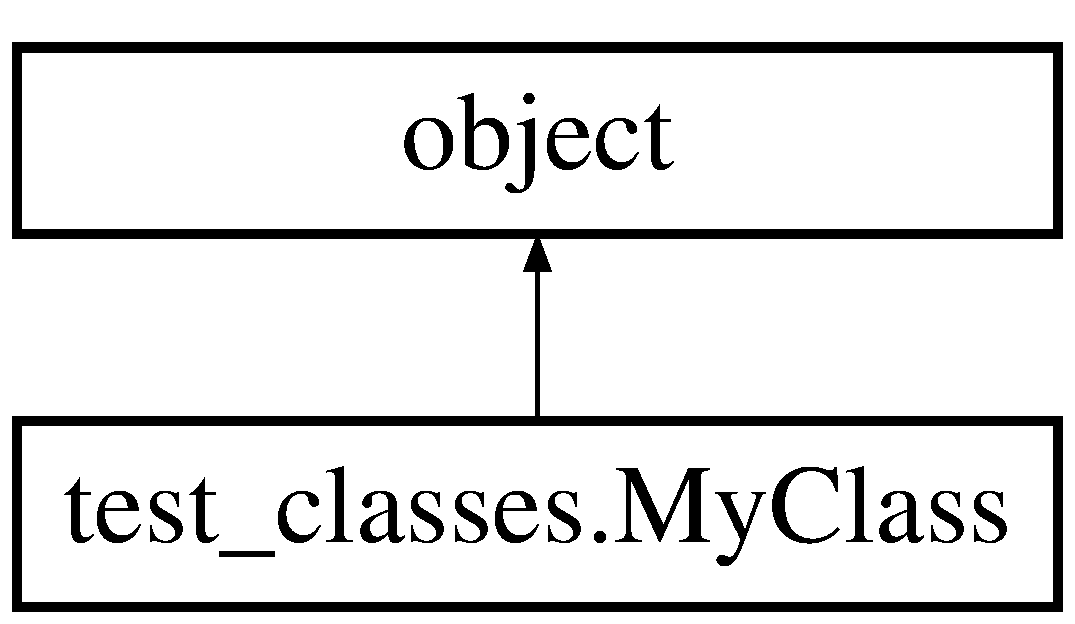
\includegraphics[height=2.000000cm]{d2/d63/classtest__classes_1_1_my_class}
\end{center}
\end{figure}
\subsection*{Public Member Functions}
\begin{DoxyCompactItemize}
\item 
def \hyperlink{classtest__classes_1_1_my_class_a7dd494c58ff3ae5f995a8ecf1face730}{\-\_\-\-\_\-init\-\_\-\-\_\-}
\item 
def \hyperlink{classtest__classes_1_1_my_class_a7886253bd105ab91453cf2a71661255b}{\-\_\-\-\_\-setattr\-\_\-\-\_\-}
\end{DoxyCompactItemize}
\subsection*{Public Attributes}
\begin{DoxyCompactItemize}
\item 
\hyperlink{classtest__classes_1_1_my_class_ad2d3f2b80c691f06bdec104b23e77cfa}{test1}
\end{DoxyCompactItemize}


\subsection{Detailed Description}


Definition at line 5 of file test\-\_\-classes.\-py.



\subsection{Constructor \& Destructor Documentation}
\hypertarget{classtest__classes_1_1_my_class_a7dd494c58ff3ae5f995a8ecf1face730}{\index{test\-\_\-classes\-::\-My\-Class@{test\-\_\-classes\-::\-My\-Class}!\-\_\-\-\_\-init\-\_\-\-\_\-@{\-\_\-\-\_\-init\-\_\-\-\_\-}}
\index{\-\_\-\-\_\-init\-\_\-\-\_\-@{\-\_\-\-\_\-init\-\_\-\-\_\-}!test_classes::MyClass@{test\-\_\-classes\-::\-My\-Class}}
\subsubsection[{\-\_\-\-\_\-init\-\_\-\-\_\-}]{\setlength{\rightskip}{0pt plus 5cm}def test\-\_\-classes.\-My\-Class.\-\_\-\-\_\-init\-\_\-\-\_\- (
\begin{DoxyParamCaption}
\item[{}]{self}
\end{DoxyParamCaption}
)}}\label{classtest__classes_1_1_my_class_a7dd494c58ff3ae5f995a8ecf1face730}


Definition at line 6 of file test\-\_\-classes.\-py.



\subsection{Member Function Documentation}
\hypertarget{classtest__classes_1_1_my_class_a7886253bd105ab91453cf2a71661255b}{\index{test\-\_\-classes\-::\-My\-Class@{test\-\_\-classes\-::\-My\-Class}!\-\_\-\-\_\-setattr\-\_\-\-\_\-@{\-\_\-\-\_\-setattr\-\_\-\-\_\-}}
\index{\-\_\-\-\_\-setattr\-\_\-\-\_\-@{\-\_\-\-\_\-setattr\-\_\-\-\_\-}!test_classes::MyClass@{test\-\_\-classes\-::\-My\-Class}}
\subsubsection[{\-\_\-\-\_\-setattr\-\_\-\-\_\-}]{\setlength{\rightskip}{0pt plus 5cm}def test\-\_\-classes.\-My\-Class.\-\_\-\-\_\-setattr\-\_\-\-\_\- (
\begin{DoxyParamCaption}
\item[{}]{self, }
\item[{}]{name, }
\item[{}]{value}
\end{DoxyParamCaption}
)}}\label{classtest__classes_1_1_my_class_a7886253bd105ab91453cf2a71661255b}


Definition at line 10 of file test\-\_\-classes.\-py.



\subsection{Member Data Documentation}
\hypertarget{classtest__classes_1_1_my_class_ad2d3f2b80c691f06bdec104b23e77cfa}{\index{test\-\_\-classes\-::\-My\-Class@{test\-\_\-classes\-::\-My\-Class}!test1@{test1}}
\index{test1@{test1}!test_classes::MyClass@{test\-\_\-classes\-::\-My\-Class}}
\subsubsection[{test1}]{\setlength{\rightskip}{0pt plus 5cm}test\-\_\-classes.\-My\-Class.\-test1}}\label{classtest__classes_1_1_my_class_ad2d3f2b80c691f06bdec104b23e77cfa}


Definition at line 7 of file test\-\_\-classes.\-py.



The documentation for this class was generated from the following file\-:\begin{DoxyCompactItemize}
\item 
amonpy/test/\hyperlink{test__classes_8py}{test\-\_\-classes.\-py}\end{DoxyCompactItemize}

\hypertarget{classtest__classes_1_1_my_class2}{\section{test\-\_\-classes.\-My\-Class2 Class Reference}
\label{classtest__classes_1_1_my_class2}\index{test\-\_\-classes.\-My\-Class2@{test\-\_\-classes.\-My\-Class2}}
}
Inheritance diagram for test\-\_\-classes.\-My\-Class2\-:\begin{figure}[H]
\begin{center}
\leavevmode
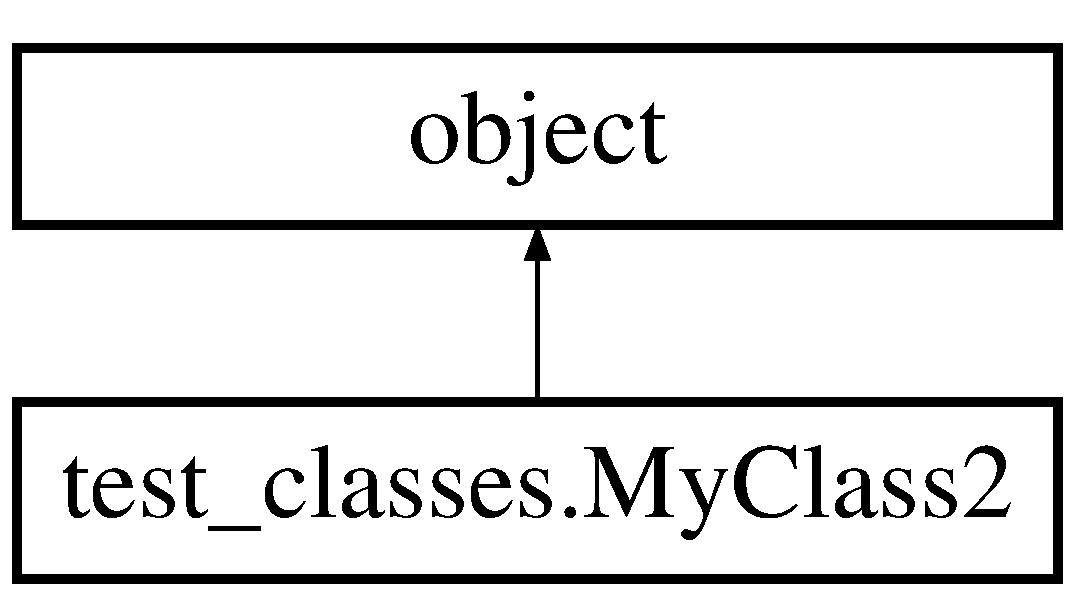
\includegraphics[height=2.000000cm]{classtest__classes_1_1_my_class2}
\end{center}
\end{figure}
\subsection*{Public Member Functions}
\begin{DoxyCompactItemize}
\item 
def \hyperlink{classtest__classes_1_1_my_class2_a277b1b75eaf63ed2a8d58583f757f6d9}{\-\_\-\-\_\-init\-\_\-\-\_\-}
\end{DoxyCompactItemize}
\subsection*{Public Attributes}
\begin{DoxyCompactItemize}
\item 
\hyperlink{classtest__classes_1_1_my_class2_aa8869bacaa7d8d98ba83bcfedd5bab49}{test1}
\end{DoxyCompactItemize}


\subsection{Constructor \& Destructor Documentation}
\hypertarget{classtest__classes_1_1_my_class2_a277b1b75eaf63ed2a8d58583f757f6d9}{\index{test\-\_\-classes\-::\-My\-Class2@{test\-\_\-classes\-::\-My\-Class2}!\-\_\-\-\_\-init\-\_\-\-\_\-@{\-\_\-\-\_\-init\-\_\-\-\_\-}}
\index{\-\_\-\-\_\-init\-\_\-\-\_\-@{\-\_\-\-\_\-init\-\_\-\-\_\-}!test_classes::MyClass2@{test\-\_\-classes\-::\-My\-Class2}}
\subsubsection[{\-\_\-\-\_\-init\-\_\-\-\_\-}]{\setlength{\rightskip}{0pt plus 5cm}def test\-\_\-classes.\-My\-Class2.\-\_\-\-\_\-init\-\_\-\-\_\- (
\begin{DoxyParamCaption}
\item[{}]{self}
\end{DoxyParamCaption}
)}}\label{classtest__classes_1_1_my_class2_a277b1b75eaf63ed2a8d58583f757f6d9}


\subsection{Member Data Documentation}
\hypertarget{classtest__classes_1_1_my_class2_aa8869bacaa7d8d98ba83bcfedd5bab49}{\index{test\-\_\-classes\-::\-My\-Class2@{test\-\_\-classes\-::\-My\-Class2}!test1@{test1}}
\index{test1@{test1}!test_classes::MyClass2@{test\-\_\-classes\-::\-My\-Class2}}
\subsubsection[{test1}]{\setlength{\rightskip}{0pt plus 5cm}test\-\_\-classes.\-My\-Class2.\-test1}}\label{classtest__classes_1_1_my_class2_aa8869bacaa7d8d98ba83bcfedd5bab49}


The documentation for this class was generated from the following file\-:\begin{DoxyCompactItemize}
\item 
amonpy/test/\hyperlink{test__classes_8py}{test\-\_\-classes.\-py}\end{DoxyCompactItemize}

\hypertarget{classgrbsim_1_1_population}{\section{grbsim.\-Population Class Reference}
\label{classgrbsim_1_1_population}\index{grbsim.\-Population@{grbsim.\-Population}}
}
Inheritance diagram for grbsim.\-Population\-:\begin{figure}[H]
\begin{center}
\leavevmode
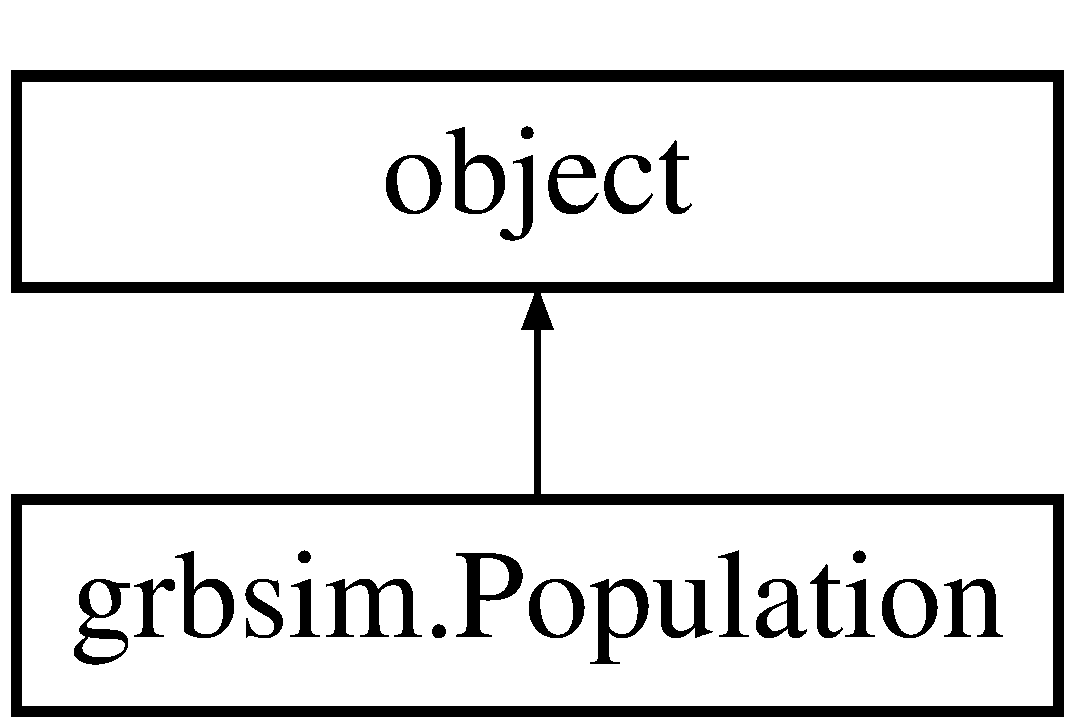
\includegraphics[height=2.000000cm]{classgrbsim_1_1_population}
\end{center}
\end{figure}
\subsection*{Public Member Functions}
\begin{DoxyCompactItemize}
\item 
def \hyperlink{classgrbsim_1_1_population_a669b24d11e789de8c0f1082969d5f1e7}{\-\_\-\-\_\-init\-\_\-\-\_\-}
\item 
def \hyperlink{classgrbsim_1_1_population_af0b9b973b441194889c09073e5e473d4}{rgrb}
\item 
def \hyperlink{classgrbsim_1_1_population_a8d0cf186fe48e6ee48e4c3242ef2b47f}{R}
\item 
def \hyperlink{classgrbsim_1_1_population_a1dc31a9ab970799cbe6aeb485fe3eb9e}{phi}
\item 
def \hyperlink{classgrbsim_1_1_population_aa004fe972bb93a589685b1ea8f4855d7}{phi\-\_\-norm}
\item 
def \hyperlink{classgrbsim_1_1_population_a7e631a73173093618e561d34b730164b}{phi\-\_\-norm2}
\item 
def \hyperlink{classgrbsim_1_1_population_a9bd7c5802bc016a63987c541831cc21a}{R\-\_\-norm}
\end{DoxyCompactItemize}
\subsection*{Public Attributes}
\begin{DoxyCompactItemize}
\item 
\hyperlink{classgrbsim_1_1_population_a142257ab80688d2ce937e9fc8e960e96}{U}
\item 
\hyperlink{classgrbsim_1_1_population_aa7e089ed973dfa3c856e9e2dc67cae48}{rho0}
\item 
\hyperlink{classgrbsim_1_1_population_a7780a80e30452b2a4682f7b6f2bf0d18}{zi}
\item 
\hyperlink{classgrbsim_1_1_population_ac6613ab254b2366c6fac7ba50e4734d7}{zf}
\item 
\hyperlink{classgrbsim_1_1_population_a2d1535d9af34a3e9355d05734e1d7c94}{z1}
\item 
\hyperlink{classgrbsim_1_1_population_a3e5dfa08846efa032f7ee66857b82b3b}{n1}
\item 
\hyperlink{classgrbsim_1_1_population_a459454cd1bb014924b82cbbce9403cca}{n2}
\item 
\hyperlink{classgrbsim_1_1_population_a33509f2091acc42103779d166c3a370c}{log\-Li}
\item 
\hyperlink{classgrbsim_1_1_population_ac24d080c569dfa5f4981ce019d17ad1a}{log\-Lf}
\item 
\hyperlink{classgrbsim_1_1_population_a9b9c750e6828e4ed66d6a052f8159a1c}{log\-L1}
\item 
\hyperlink{classgrbsim_1_1_population_a3bd729ea7c1a389c8d6377506e2de622}{alpha}
\item 
\hyperlink{classgrbsim_1_1_population_ae00d66b8505071bc2d0c9e9dee32223c}{beta}
\end{DoxyCompactItemize}


\subsection{Constructor \& Destructor Documentation}
\hypertarget{classgrbsim_1_1_population_a669b24d11e789de8c0f1082969d5f1e7}{\index{grbsim\-::\-Population@{grbsim\-::\-Population}!\-\_\-\-\_\-init\-\_\-\-\_\-@{\-\_\-\-\_\-init\-\_\-\-\_\-}}
\index{\-\_\-\-\_\-init\-\_\-\-\_\-@{\-\_\-\-\_\-init\-\_\-\-\_\-}!grbsim::Population@{grbsim\-::\-Population}}
\subsubsection[{\-\_\-\-\_\-init\-\_\-\-\_\-}]{\setlength{\rightskip}{0pt plus 5cm}def grbsim.\-Population.\-\_\-\-\_\-init\-\_\-\-\_\- (
\begin{DoxyParamCaption}
\item[{}]{self, }
\item[{}]{rho0, }
\item[{}]{zi, }
\item[{}]{zf, }
\item[{}]{z1, }
\item[{}]{n1, }
\item[{}]{n2, }
\item[{}]{log\-Li, }
\item[{}]{log\-Lf, }
\item[{}]{log\-L1, }
\item[{}]{alpha, }
\item[{}]{beta, }
\item[{}]{U}
\end{DoxyParamCaption}
)}}\label{classgrbsim_1_1_population_a669b24d11e789de8c0f1082969d5f1e7}


\subsection{Member Function Documentation}
\hypertarget{classgrbsim_1_1_population_a1dc31a9ab970799cbe6aeb485fe3eb9e}{\index{grbsim\-::\-Population@{grbsim\-::\-Population}!phi@{phi}}
\index{phi@{phi}!grbsim::Population@{grbsim\-::\-Population}}
\subsubsection[{phi}]{\setlength{\rightskip}{0pt plus 5cm}def grbsim.\-Population.\-phi (
\begin{DoxyParamCaption}
\item[{}]{self, }
\item[{}]{log\-L}
\end{DoxyParamCaption}
)}}\label{classgrbsim_1_1_population_a1dc31a9ab970799cbe6aeb485fe3eb9e}
\hypertarget{classgrbsim_1_1_population_aa004fe972bb93a589685b1ea8f4855d7}{\index{grbsim\-::\-Population@{grbsim\-::\-Population}!phi\-\_\-norm@{phi\-\_\-norm}}
\index{phi\-\_\-norm@{phi\-\_\-norm}!grbsim::Population@{grbsim\-::\-Population}}
\subsubsection[{phi\-\_\-norm}]{\setlength{\rightskip}{0pt plus 5cm}def grbsim.\-Population.\-phi\-\_\-norm (
\begin{DoxyParamCaption}
\item[{}]{self}
\end{DoxyParamCaption}
)}}\label{classgrbsim_1_1_population_aa004fe972bb93a589685b1ea8f4855d7}
\hypertarget{classgrbsim_1_1_population_a7e631a73173093618e561d34b730164b}{\index{grbsim\-::\-Population@{grbsim\-::\-Population}!phi\-\_\-norm2@{phi\-\_\-norm2}}
\index{phi\-\_\-norm2@{phi\-\_\-norm2}!grbsim::Population@{grbsim\-::\-Population}}
\subsubsection[{phi\-\_\-norm2}]{\setlength{\rightskip}{0pt plus 5cm}def grbsim.\-Population.\-phi\-\_\-norm2 (
\begin{DoxyParamCaption}
\item[{}]{self}
\end{DoxyParamCaption}
)}}\label{classgrbsim_1_1_population_a7e631a73173093618e561d34b730164b}
\hypertarget{classgrbsim_1_1_population_a8d0cf186fe48e6ee48e4c3242ef2b47f}{\index{grbsim\-::\-Population@{grbsim\-::\-Population}!R@{R}}
\index{R@{R}!grbsim::Population@{grbsim\-::\-Population}}
\subsubsection[{R}]{\setlength{\rightskip}{0pt plus 5cm}def grbsim.\-Population.\-R (
\begin{DoxyParamCaption}
\item[{}]{self, }
\item[{}]{z}
\end{DoxyParamCaption}
)}}\label{classgrbsim_1_1_population_a8d0cf186fe48e6ee48e4c3242ef2b47f}
\hypertarget{classgrbsim_1_1_population_a9bd7c5802bc016a63987c541831cc21a}{\index{grbsim\-::\-Population@{grbsim\-::\-Population}!R\-\_\-norm@{R\-\_\-norm}}
\index{R\-\_\-norm@{R\-\_\-norm}!grbsim::Population@{grbsim\-::\-Population}}
\subsubsection[{R\-\_\-norm}]{\setlength{\rightskip}{0pt plus 5cm}def grbsim.\-Population.\-R\-\_\-norm (
\begin{DoxyParamCaption}
\item[{}]{self}
\end{DoxyParamCaption}
)}}\label{classgrbsim_1_1_population_a9bd7c5802bc016a63987c541831cc21a}
\hypertarget{classgrbsim_1_1_population_af0b9b973b441194889c09073e5e473d4}{\index{grbsim\-::\-Population@{grbsim\-::\-Population}!rgrb@{rgrb}}
\index{rgrb@{rgrb}!grbsim::Population@{grbsim\-::\-Population}}
\subsubsection[{rgrb}]{\setlength{\rightskip}{0pt plus 5cm}def grbsim.\-Population.\-rgrb (
\begin{DoxyParamCaption}
\item[{}]{self, }
\item[{}]{z}
\end{DoxyParamCaption}
)}}\label{classgrbsim_1_1_population_af0b9b973b441194889c09073e5e473d4}


\subsection{Member Data Documentation}
\hypertarget{classgrbsim_1_1_population_a3bd729ea7c1a389c8d6377506e2de622}{\index{grbsim\-::\-Population@{grbsim\-::\-Population}!alpha@{alpha}}
\index{alpha@{alpha}!grbsim::Population@{grbsim\-::\-Population}}
\subsubsection[{alpha}]{\setlength{\rightskip}{0pt plus 5cm}grbsim.\-Population.\-alpha}}\label{classgrbsim_1_1_population_a3bd729ea7c1a389c8d6377506e2de622}
\hypertarget{classgrbsim_1_1_population_ae00d66b8505071bc2d0c9e9dee32223c}{\index{grbsim\-::\-Population@{grbsim\-::\-Population}!beta@{beta}}
\index{beta@{beta}!grbsim::Population@{grbsim\-::\-Population}}
\subsubsection[{beta}]{\setlength{\rightskip}{0pt plus 5cm}grbsim.\-Population.\-beta}}\label{classgrbsim_1_1_population_ae00d66b8505071bc2d0c9e9dee32223c}
\hypertarget{classgrbsim_1_1_population_a9b9c750e6828e4ed66d6a052f8159a1c}{\index{grbsim\-::\-Population@{grbsim\-::\-Population}!log\-L1@{log\-L1}}
\index{log\-L1@{log\-L1}!grbsim::Population@{grbsim\-::\-Population}}
\subsubsection[{log\-L1}]{\setlength{\rightskip}{0pt plus 5cm}grbsim.\-Population.\-log\-L1}}\label{classgrbsim_1_1_population_a9b9c750e6828e4ed66d6a052f8159a1c}
\hypertarget{classgrbsim_1_1_population_ac24d080c569dfa5f4981ce019d17ad1a}{\index{grbsim\-::\-Population@{grbsim\-::\-Population}!log\-Lf@{log\-Lf}}
\index{log\-Lf@{log\-Lf}!grbsim::Population@{grbsim\-::\-Population}}
\subsubsection[{log\-Lf}]{\setlength{\rightskip}{0pt plus 5cm}grbsim.\-Population.\-log\-Lf}}\label{classgrbsim_1_1_population_ac24d080c569dfa5f4981ce019d17ad1a}
\hypertarget{classgrbsim_1_1_population_a33509f2091acc42103779d166c3a370c}{\index{grbsim\-::\-Population@{grbsim\-::\-Population}!log\-Li@{log\-Li}}
\index{log\-Li@{log\-Li}!grbsim::Population@{grbsim\-::\-Population}}
\subsubsection[{log\-Li}]{\setlength{\rightskip}{0pt plus 5cm}grbsim.\-Population.\-log\-Li}}\label{classgrbsim_1_1_population_a33509f2091acc42103779d166c3a370c}
\hypertarget{classgrbsim_1_1_population_a3e5dfa08846efa032f7ee66857b82b3b}{\index{grbsim\-::\-Population@{grbsim\-::\-Population}!n1@{n1}}
\index{n1@{n1}!grbsim::Population@{grbsim\-::\-Population}}
\subsubsection[{n1}]{\setlength{\rightskip}{0pt plus 5cm}grbsim.\-Population.\-n1}}\label{classgrbsim_1_1_population_a3e5dfa08846efa032f7ee66857b82b3b}
\hypertarget{classgrbsim_1_1_population_a459454cd1bb014924b82cbbce9403cca}{\index{grbsim\-::\-Population@{grbsim\-::\-Population}!n2@{n2}}
\index{n2@{n2}!grbsim::Population@{grbsim\-::\-Population}}
\subsubsection[{n2}]{\setlength{\rightskip}{0pt plus 5cm}grbsim.\-Population.\-n2}}\label{classgrbsim_1_1_population_a459454cd1bb014924b82cbbce9403cca}
\hypertarget{classgrbsim_1_1_population_aa7e089ed973dfa3c856e9e2dc67cae48}{\index{grbsim\-::\-Population@{grbsim\-::\-Population}!rho0@{rho0}}
\index{rho0@{rho0}!grbsim::Population@{grbsim\-::\-Population}}
\subsubsection[{rho0}]{\setlength{\rightskip}{0pt plus 5cm}grbsim.\-Population.\-rho0}}\label{classgrbsim_1_1_population_aa7e089ed973dfa3c856e9e2dc67cae48}
\hypertarget{classgrbsim_1_1_population_a142257ab80688d2ce937e9fc8e960e96}{\index{grbsim\-::\-Population@{grbsim\-::\-Population}!U@{U}}
\index{U@{U}!grbsim::Population@{grbsim\-::\-Population}}
\subsubsection[{U}]{\setlength{\rightskip}{0pt plus 5cm}grbsim.\-Population.\-U}}\label{classgrbsim_1_1_population_a142257ab80688d2ce937e9fc8e960e96}
\hypertarget{classgrbsim_1_1_population_a2d1535d9af34a3e9355d05734e1d7c94}{\index{grbsim\-::\-Population@{grbsim\-::\-Population}!z1@{z1}}
\index{z1@{z1}!grbsim::Population@{grbsim\-::\-Population}}
\subsubsection[{z1}]{\setlength{\rightskip}{0pt plus 5cm}grbsim.\-Population.\-z1}}\label{classgrbsim_1_1_population_a2d1535d9af34a3e9355d05734e1d7c94}
\hypertarget{classgrbsim_1_1_population_ac6613ab254b2366c6fac7ba50e4734d7}{\index{grbsim\-::\-Population@{grbsim\-::\-Population}!zf@{zf}}
\index{zf@{zf}!grbsim::Population@{grbsim\-::\-Population}}
\subsubsection[{zf}]{\setlength{\rightskip}{0pt plus 5cm}grbsim.\-Population.\-zf}}\label{classgrbsim_1_1_population_ac6613ab254b2366c6fac7ba50e4734d7}
\hypertarget{classgrbsim_1_1_population_a7780a80e30452b2a4682f7b6f2bf0d18}{\index{grbsim\-::\-Population@{grbsim\-::\-Population}!zi@{zi}}
\index{zi@{zi}!grbsim::Population@{grbsim\-::\-Population}}
\subsubsection[{zi}]{\setlength{\rightskip}{0pt plus 5cm}grbsim.\-Population.\-zi}}\label{classgrbsim_1_1_population_a7780a80e30452b2a4682f7b6f2bf0d18}


The documentation for this class was generated from the following file\-:\begin{DoxyCompactItemize}
\item 
amonpy/sim/sources/\hyperlink{grbsim_8py}{grbsim.\-py}\end{DoxyCompactItemize}

\hypertarget{classamonpy_1_1sim_1_1sidereal_1_1_r_a_dec}{\section{amonpy.\-sim.\-sidereal.\-R\-A\-Dec Class Reference}
\label{classamonpy_1_1sim_1_1sidereal_1_1_r_a_dec}\index{amonpy.\-sim.\-sidereal.\-R\-A\-Dec@{amonpy.\-sim.\-sidereal.\-R\-A\-Dec}}
}
\subsection*{Public Member Functions}
\begin{DoxyCompactItemize}
\item 
def \hyperlink{classamonpy_1_1sim_1_1sidereal_1_1_r_a_dec_a7fcc52d232c37e4100801dac5937bf07}{\-\_\-\-\_\-init\-\_\-\-\_\-}
\item 
def \hyperlink{classamonpy_1_1sim_1_1sidereal_1_1_r_a_dec_a0c665408ad8904cad5a4a4fe2fcb59c6}{hour\-Angle}
\item 
def \hyperlink{classamonpy_1_1sim_1_1sidereal_1_1_r_a_dec_aa6fd908114d65acf9cc93d00ff265ef7}{alt\-Az}
\item 
def \hyperlink{classamonpy_1_1sim_1_1sidereal_1_1_r_a_dec_a34138720c66b6790006018fb43cd0f5f}{\-\_\-\-\_\-str\-\_\-\-\_\-}
\end{DoxyCompactItemize}
\subsection*{Public Attributes}
\begin{DoxyCompactItemize}
\item 
\hyperlink{classamonpy_1_1sim_1_1sidereal_1_1_r_a_dec_aa2e5e1ae8fb268048785320c22e6aef3}{ra}
\item 
\hyperlink{classamonpy_1_1sim_1_1sidereal_1_1_r_a_dec_a02fc3786821a861ab339dd1d6f04d9bd}{dec}
\end{DoxyCompactItemize}


\subsection{Detailed Description}
\begin{DoxyVerb}Represents a celestial location in equatorial coordinates.

  Exports/Invariants:
    .ra:      [ right ascension in radians ]
    .dec:     [ declination in radians ]
\end{DoxyVerb}
 

\subsection{Constructor \& Destructor Documentation}
\hypertarget{classamonpy_1_1sim_1_1sidereal_1_1_r_a_dec_a7fcc52d232c37e4100801dac5937bf07}{\index{amonpy\-::sim\-::sidereal\-::\-R\-A\-Dec@{amonpy\-::sim\-::sidereal\-::\-R\-A\-Dec}!\-\_\-\-\_\-init\-\_\-\-\_\-@{\-\_\-\-\_\-init\-\_\-\-\_\-}}
\index{\-\_\-\-\_\-init\-\_\-\-\_\-@{\-\_\-\-\_\-init\-\_\-\-\_\-}!amonpy::sim::sidereal::RADec@{amonpy\-::sim\-::sidereal\-::\-R\-A\-Dec}}
\subsubsection[{\-\_\-\-\_\-init\-\_\-\-\_\-}]{\setlength{\rightskip}{0pt plus 5cm}def amonpy.\-sim.\-sidereal.\-R\-A\-Dec.\-\_\-\-\_\-init\-\_\-\-\_\- (
\begin{DoxyParamCaption}
\item[{}]{self, }
\item[{}]{ra, }
\item[{}]{dec}
\end{DoxyParamCaption}
)}}\label{classamonpy_1_1sim_1_1sidereal_1_1_r_a_dec_a7fcc52d232c37e4100801dac5937bf07}
\begin{DoxyVerb}Constructor for RADec.
\end{DoxyVerb}
 

\subsection{Member Function Documentation}
\hypertarget{classamonpy_1_1sim_1_1sidereal_1_1_r_a_dec_a34138720c66b6790006018fb43cd0f5f}{\index{amonpy\-::sim\-::sidereal\-::\-R\-A\-Dec@{amonpy\-::sim\-::sidereal\-::\-R\-A\-Dec}!\-\_\-\-\_\-str\-\_\-\-\_\-@{\-\_\-\-\_\-str\-\_\-\-\_\-}}
\index{\-\_\-\-\_\-str\-\_\-\-\_\-@{\-\_\-\-\_\-str\-\_\-\-\_\-}!amonpy::sim::sidereal::RADec@{amonpy\-::sim\-::sidereal\-::\-R\-A\-Dec}}
\subsubsection[{\-\_\-\-\_\-str\-\_\-\-\_\-}]{\setlength{\rightskip}{0pt plus 5cm}def amonpy.\-sim.\-sidereal.\-R\-A\-Dec.\-\_\-\-\_\-str\-\_\-\-\_\- (
\begin{DoxyParamCaption}
\item[{}]{self}
\end{DoxyParamCaption}
)}}\label{classamonpy_1_1sim_1_1sidereal_1_1_r_a_dec_a34138720c66b6790006018fb43cd0f5f}
\begin{DoxyVerb}Return self as a string.
\end{DoxyVerb}
 \hypertarget{classamonpy_1_1sim_1_1sidereal_1_1_r_a_dec_aa6fd908114d65acf9cc93d00ff265ef7}{\index{amonpy\-::sim\-::sidereal\-::\-R\-A\-Dec@{amonpy\-::sim\-::sidereal\-::\-R\-A\-Dec}!alt\-Az@{alt\-Az}}
\index{alt\-Az@{alt\-Az}!amonpy::sim::sidereal::RADec@{amonpy\-::sim\-::sidereal\-::\-R\-A\-Dec}}
\subsubsection[{alt\-Az}]{\setlength{\rightskip}{0pt plus 5cm}def amonpy.\-sim.\-sidereal.\-R\-A\-Dec.\-alt\-Az (
\begin{DoxyParamCaption}
\item[{}]{self, }
\item[{}]{h, }
\item[{}]{lat}
\end{DoxyParamCaption}
)}}\label{classamonpy_1_1sim_1_1sidereal_1_1_r_a_dec_aa6fd908114d65acf9cc93d00ff265ef7}
\begin{DoxyVerb}Convert equatorial to horizon coordinates.

  [ (h is an object's hour angle in radians) and
    (lat is the observer's latitude in radians) ->
      return self's position in the observer's sky
      in horizon coordinates as an AltAz instance ]
\end{DoxyVerb}
 \hypertarget{classamonpy_1_1sim_1_1sidereal_1_1_r_a_dec_a0c665408ad8904cad5a4a4fe2fcb59c6}{\index{amonpy\-::sim\-::sidereal\-::\-R\-A\-Dec@{amonpy\-::sim\-::sidereal\-::\-R\-A\-Dec}!hour\-Angle@{hour\-Angle}}
\index{hour\-Angle@{hour\-Angle}!amonpy::sim::sidereal::RADec@{amonpy\-::sim\-::sidereal\-::\-R\-A\-Dec}}
\subsubsection[{hour\-Angle}]{\setlength{\rightskip}{0pt plus 5cm}def amonpy.\-sim.\-sidereal.\-R\-A\-Dec.\-hour\-Angle (
\begin{DoxyParamCaption}
\item[{}]{self, }
\item[{}]{utc, }
\item[{}]{e\-Long}
\end{DoxyParamCaption}
)}}\label{classamonpy_1_1sim_1_1sidereal_1_1_r_a_dec_a0c665408ad8904cad5a4a4fe2fcb59c6}
\begin{DoxyVerb}Find the hour angle at a given observer's location.

  [ (utc is a Universal Time as a datetime.datetime) and
    (eLong is an east longitude in radians) ->
      return the hour angle of self at that time and
      longitude, in radians ]
\end{DoxyVerb}
 

\subsection{Member Data Documentation}
\hypertarget{classamonpy_1_1sim_1_1sidereal_1_1_r_a_dec_a02fc3786821a861ab339dd1d6f04d9bd}{\index{amonpy\-::sim\-::sidereal\-::\-R\-A\-Dec@{amonpy\-::sim\-::sidereal\-::\-R\-A\-Dec}!dec@{dec}}
\index{dec@{dec}!amonpy::sim::sidereal::RADec@{amonpy\-::sim\-::sidereal\-::\-R\-A\-Dec}}
\subsubsection[{dec}]{\setlength{\rightskip}{0pt plus 5cm}amonpy.\-sim.\-sidereal.\-R\-A\-Dec.\-dec}}\label{classamonpy_1_1sim_1_1sidereal_1_1_r_a_dec_a02fc3786821a861ab339dd1d6f04d9bd}
\hypertarget{classamonpy_1_1sim_1_1sidereal_1_1_r_a_dec_aa2e5e1ae8fb268048785320c22e6aef3}{\index{amonpy\-::sim\-::sidereal\-::\-R\-A\-Dec@{amonpy\-::sim\-::sidereal\-::\-R\-A\-Dec}!ra@{ra}}
\index{ra@{ra}!amonpy::sim::sidereal::RADec@{amonpy\-::sim\-::sidereal\-::\-R\-A\-Dec}}
\subsubsection[{ra}]{\setlength{\rightskip}{0pt plus 5cm}amonpy.\-sim.\-sidereal.\-R\-A\-Dec.\-ra}}\label{classamonpy_1_1sim_1_1sidereal_1_1_r_a_dec_aa2e5e1ae8fb268048785320c22e6aef3}


The documentation for this class was generated from the following file\-:\begin{DoxyCompactItemize}
\item 
amonpy/sim/\hyperlink{sidereal_8py}{sidereal.\-py}\end{DoxyCompactItemize}

\hypertarget{classamonpy_1_1sim_1_1sidereal__m_1_1_r_a_dec}{\section{amonpy.\-sim.\-sidereal\-\_\-m.\-R\-A\-Dec Class Reference}
\label{classamonpy_1_1sim_1_1sidereal__m_1_1_r_a_dec}\index{amonpy.\-sim.\-sidereal\-\_\-m.\-R\-A\-Dec@{amonpy.\-sim.\-sidereal\-\_\-m.\-R\-A\-Dec}}
}


Represents a celestial location in equatorial coordinates.  




\subsection{Detailed Description}
Represents a celestial location in equatorial coordinates. 

Exports/\-Invariants\-: .ra\-: \mbox{[} right ascension in radians \mbox{]} .dec\-: \mbox{[} declination in radians \mbox{]} 

Definition at line 1473 of file sidereal\-\_\-m.\-py.



The documentation for this class was generated from the following file\-:\begin{DoxyCompactItemize}
\item 
amonpy/sim/\hyperlink{sidereal__m_8py}{sidereal\-\_\-m.\-py}\end{DoxyCompactItemize}

\hypertarget{classamonpy_1_1tools_1_1input__text__window_1_1_select_choice}{\section{amonpy.\-tools.\-input\-\_\-text\-\_\-window.\-Select\-Choice Class Reference}
\label{classamonpy_1_1tools_1_1input__text__window_1_1_select_choice}\index{amonpy.\-tools.\-input\-\_\-text\-\_\-window.\-Select\-Choice@{amonpy.\-tools.\-input\-\_\-text\-\_\-window.\-Select\-Choice}}
}
Inheritance diagram for amonpy.\-tools.\-input\-\_\-text\-\_\-window.\-Select\-Choice\-:\begin{figure}[H]
\begin{center}
\leavevmode
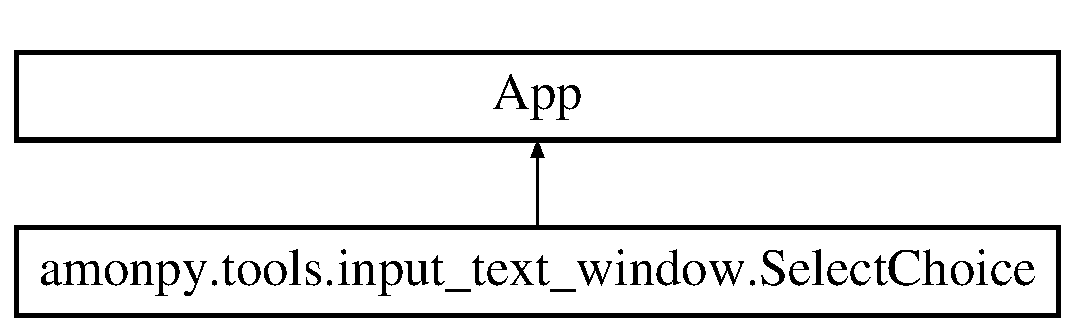
\includegraphics[height=2.000000cm]{classamonpy_1_1tools_1_1input__text__window_1_1_select_choice}
\end{center}
\end{figure}
\subsection*{Public Member Functions}
\begin{DoxyCompactItemize}
\item 
def \hyperlink{classamonpy_1_1tools_1_1input__text__window_1_1_select_choice_aedbd4663dd0e28caf001585c390072ca}{\-\_\-\-\_\-init\-\_\-\-\_\-}
\item 
def \hyperlink{classamonpy_1_1tools_1_1input__text__window_1_1_select_choice_a46b3d909cca619c1489e4d1f4080e36a}{on\-\_\-click\-\_\-or\-\_\-close}
\item 
def \hyperlink{classamonpy_1_1tools_1_1input__text__window_1_1_select_choice_a847223a6204d1851aedcde1c2b88cccf}{result}
\end{DoxyCompactItemize}
\subsection*{Public Attributes}
\begin{DoxyCompactItemize}
\item 
\hyperlink{classamonpy_1_1tools_1_1input__text__window_1_1_select_choice_aa47ee685de6c28e23b244fdae0eaad87}{info}
\item 
\hyperlink{classamonpy_1_1tools_1_1input__text__window_1_1_select_choice_aee9b6e27856594efa52216a82b62521e}{frame}
\item 
\hyperlink{classamonpy_1_1tools_1_1input__text__window_1_1_select_choice_a6983cf49c1516c4653cad8e3663dbb38}{text}
\item 
\hyperlink{classamonpy_1_1tools_1_1input__text__window_1_1_select_choice_aab6b0771ae4ce1d7f51e5a7cd8cb3c3d}{text\-Ctrl1}
\item 
\hyperlink{classamonpy_1_1tools_1_1input__text__window_1_1_select_choice_acc99d030bfd068e7f24d6d77f5c5c767}{button}
\end{DoxyCompactItemize}


\subsection{Constructor \& Destructor Documentation}
\hypertarget{classamonpy_1_1tools_1_1input__text__window_1_1_select_choice_aedbd4663dd0e28caf001585c390072ca}{\index{amonpy\-::tools\-::input\-\_\-text\-\_\-window\-::\-Select\-Choice@{amonpy\-::tools\-::input\-\_\-text\-\_\-window\-::\-Select\-Choice}!\-\_\-\-\_\-init\-\_\-\-\_\-@{\-\_\-\-\_\-init\-\_\-\-\_\-}}
\index{\-\_\-\-\_\-init\-\_\-\-\_\-@{\-\_\-\-\_\-init\-\_\-\-\_\-}!amonpy::tools::input_text_window::SelectChoice@{amonpy\-::tools\-::input\-\_\-text\-\_\-window\-::\-Select\-Choice}}
\subsubsection[{\-\_\-\-\_\-init\-\_\-\-\_\-}]{\setlength{\rightskip}{0pt plus 5cm}def amonpy.\-tools.\-input\-\_\-text\-\_\-window.\-Select\-Choice.\-\_\-\-\_\-init\-\_\-\-\_\- (
\begin{DoxyParamCaption}
\item[{}]{self, }
\item[{}]{kwargs}
\end{DoxyParamCaption}
)}}\label{classamonpy_1_1tools_1_1input__text__window_1_1_select_choice_aedbd4663dd0e28caf001585c390072ca}


\subsection{Member Function Documentation}
\hypertarget{classamonpy_1_1tools_1_1input__text__window_1_1_select_choice_a46b3d909cca619c1489e4d1f4080e36a}{\index{amonpy\-::tools\-::input\-\_\-text\-\_\-window\-::\-Select\-Choice@{amonpy\-::tools\-::input\-\_\-text\-\_\-window\-::\-Select\-Choice}!on\-\_\-click\-\_\-or\-\_\-close@{on\-\_\-click\-\_\-or\-\_\-close}}
\index{on\-\_\-click\-\_\-or\-\_\-close@{on\-\_\-click\-\_\-or\-\_\-close}!amonpy::tools::input_text_window::SelectChoice@{amonpy\-::tools\-::input\-\_\-text\-\_\-window\-::\-Select\-Choice}}
\subsubsection[{on\-\_\-click\-\_\-or\-\_\-close}]{\setlength{\rightskip}{0pt plus 5cm}def amonpy.\-tools.\-input\-\_\-text\-\_\-window.\-Select\-Choice.\-on\-\_\-click\-\_\-or\-\_\-close (
\begin{DoxyParamCaption}
\item[{}]{self, }
\item[{}]{event}
\end{DoxyParamCaption}
)}}\label{classamonpy_1_1tools_1_1input__text__window_1_1_select_choice_a46b3d909cca619c1489e4d1f4080e36a}
\hypertarget{classamonpy_1_1tools_1_1input__text__window_1_1_select_choice_a847223a6204d1851aedcde1c2b88cccf}{\index{amonpy\-::tools\-::input\-\_\-text\-\_\-window\-::\-Select\-Choice@{amonpy\-::tools\-::input\-\_\-text\-\_\-window\-::\-Select\-Choice}!result@{result}}
\index{result@{result}!amonpy::tools::input_text_window::SelectChoice@{amonpy\-::tools\-::input\-\_\-text\-\_\-window\-::\-Select\-Choice}}
\subsubsection[{result}]{\setlength{\rightskip}{0pt plus 5cm}def amonpy.\-tools.\-input\-\_\-text\-\_\-window.\-Select\-Choice.\-result (
\begin{DoxyParamCaption}
\item[{}]{self}
\end{DoxyParamCaption}
)}}\label{classamonpy_1_1tools_1_1input__text__window_1_1_select_choice_a847223a6204d1851aedcde1c2b88cccf}


\subsection{Member Data Documentation}
\hypertarget{classamonpy_1_1tools_1_1input__text__window_1_1_select_choice_acc99d030bfd068e7f24d6d77f5c5c767}{\index{amonpy\-::tools\-::input\-\_\-text\-\_\-window\-::\-Select\-Choice@{amonpy\-::tools\-::input\-\_\-text\-\_\-window\-::\-Select\-Choice}!button@{button}}
\index{button@{button}!amonpy::tools::input_text_window::SelectChoice@{amonpy\-::tools\-::input\-\_\-text\-\_\-window\-::\-Select\-Choice}}
\subsubsection[{button}]{\setlength{\rightskip}{0pt plus 5cm}amonpy.\-tools.\-input\-\_\-text\-\_\-window.\-Select\-Choice.\-button}}\label{classamonpy_1_1tools_1_1input__text__window_1_1_select_choice_acc99d030bfd068e7f24d6d77f5c5c767}
\hypertarget{classamonpy_1_1tools_1_1input__text__window_1_1_select_choice_aee9b6e27856594efa52216a82b62521e}{\index{amonpy\-::tools\-::input\-\_\-text\-\_\-window\-::\-Select\-Choice@{amonpy\-::tools\-::input\-\_\-text\-\_\-window\-::\-Select\-Choice}!frame@{frame}}
\index{frame@{frame}!amonpy::tools::input_text_window::SelectChoice@{amonpy\-::tools\-::input\-\_\-text\-\_\-window\-::\-Select\-Choice}}
\subsubsection[{frame}]{\setlength{\rightskip}{0pt plus 5cm}amonpy.\-tools.\-input\-\_\-text\-\_\-window.\-Select\-Choice.\-frame}}\label{classamonpy_1_1tools_1_1input__text__window_1_1_select_choice_aee9b6e27856594efa52216a82b62521e}
\hypertarget{classamonpy_1_1tools_1_1input__text__window_1_1_select_choice_aa47ee685de6c28e23b244fdae0eaad87}{\index{amonpy\-::tools\-::input\-\_\-text\-\_\-window\-::\-Select\-Choice@{amonpy\-::tools\-::input\-\_\-text\-\_\-window\-::\-Select\-Choice}!info@{info}}
\index{info@{info}!amonpy::tools::input_text_window::SelectChoice@{amonpy\-::tools\-::input\-\_\-text\-\_\-window\-::\-Select\-Choice}}
\subsubsection[{info}]{\setlength{\rightskip}{0pt plus 5cm}amonpy.\-tools.\-input\-\_\-text\-\_\-window.\-Select\-Choice.\-info}}\label{classamonpy_1_1tools_1_1input__text__window_1_1_select_choice_aa47ee685de6c28e23b244fdae0eaad87}
\hypertarget{classamonpy_1_1tools_1_1input__text__window_1_1_select_choice_a6983cf49c1516c4653cad8e3663dbb38}{\index{amonpy\-::tools\-::input\-\_\-text\-\_\-window\-::\-Select\-Choice@{amonpy\-::tools\-::input\-\_\-text\-\_\-window\-::\-Select\-Choice}!text@{text}}
\index{text@{text}!amonpy::tools::input_text_window::SelectChoice@{amonpy\-::tools\-::input\-\_\-text\-\_\-window\-::\-Select\-Choice}}
\subsubsection[{text}]{\setlength{\rightskip}{0pt plus 5cm}amonpy.\-tools.\-input\-\_\-text\-\_\-window.\-Select\-Choice.\-text}}\label{classamonpy_1_1tools_1_1input__text__window_1_1_select_choice_a6983cf49c1516c4653cad8e3663dbb38}
\hypertarget{classamonpy_1_1tools_1_1input__text__window_1_1_select_choice_aab6b0771ae4ce1d7f51e5a7cd8cb3c3d}{\index{amonpy\-::tools\-::input\-\_\-text\-\_\-window\-::\-Select\-Choice@{amonpy\-::tools\-::input\-\_\-text\-\_\-window\-::\-Select\-Choice}!text\-Ctrl1@{text\-Ctrl1}}
\index{text\-Ctrl1@{text\-Ctrl1}!amonpy::tools::input_text_window::SelectChoice@{amonpy\-::tools\-::input\-\_\-text\-\_\-window\-::\-Select\-Choice}}
\subsubsection[{text\-Ctrl1}]{\setlength{\rightskip}{0pt plus 5cm}amonpy.\-tools.\-input\-\_\-text\-\_\-window.\-Select\-Choice.\-text\-Ctrl1}}\label{classamonpy_1_1tools_1_1input__text__window_1_1_select_choice_aab6b0771ae4ce1d7f51e5a7cd8cb3c3d}


The documentation for this class was generated from the following file\-:\begin{DoxyCompactItemize}
\item 
amonpy/tools/\hyperlink{input__text__window_8py}{input\-\_\-text\-\_\-window.\-py}\end{DoxyCompactItemize}

\hypertarget{classamonpy_1_1tools_1_1dialog__choice_1_1_select_choice}{\section{amonpy.\-tools.\-dialog\-\_\-choice.\-Select\-Choice Class Reference}
\label{classamonpy_1_1tools_1_1dialog__choice_1_1_select_choice}\index{amonpy.\-tools.\-dialog\-\_\-choice.\-Select\-Choice@{amonpy.\-tools.\-dialog\-\_\-choice.\-Select\-Choice}}
}
Inheritance diagram for amonpy.\-tools.\-dialog\-\_\-choice.\-Select\-Choice\-:\begin{figure}[H]
\begin{center}
\leavevmode
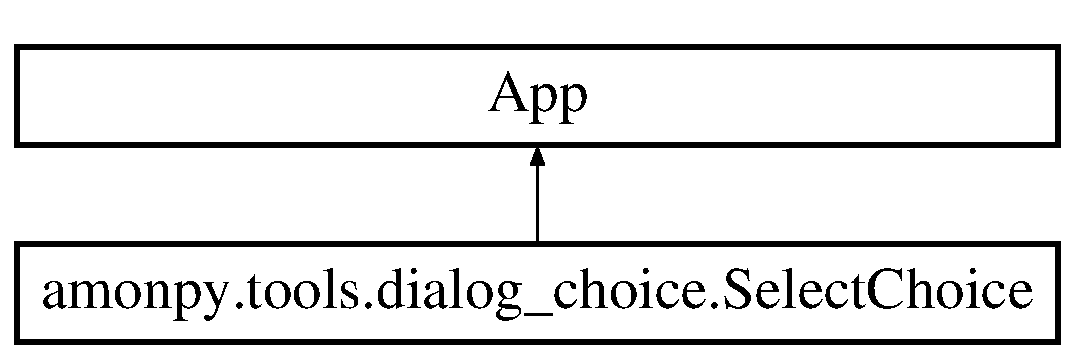
\includegraphics[height=2.000000cm]{classamonpy_1_1tools_1_1dialog__choice_1_1_select_choice}
\end{center}
\end{figure}
\subsection*{Public Member Functions}
\begin{DoxyCompactItemize}
\item 
def \hyperlink{classamonpy_1_1tools_1_1dialog__choice_1_1_select_choice_a9ffb7fd1e40656e936f4485e5c3b3c6e}{\-\_\-\-\_\-init\-\_\-\-\_\-}
\item 
def \hyperlink{classamonpy_1_1tools_1_1dialog__choice_1_1_select_choice_ac31e6372528c3039e831163f6e6bb939}{on\-\_\-click\-\_\-or\-\_\-close}
\item 
def \hyperlink{classamonpy_1_1tools_1_1dialog__choice_1_1_select_choice_a8bca0cecf2d89c6936849f69671d9945}{result}
\end{DoxyCompactItemize}
\subsection*{Public Attributes}
\begin{DoxyCompactItemize}
\item 
\hyperlink{classamonpy_1_1tools_1_1dialog__choice_1_1_select_choice_a8363438c3e75f765ca4b2c98eaf26699}{choices}
\item 
\hyperlink{classamonpy_1_1tools_1_1dialog__choice_1_1_select_choice_ab2d0390c17c73e14838add2d52d0f73d}{info}
\item 
\hyperlink{classamonpy_1_1tools_1_1dialog__choice_1_1_select_choice_a177ab137db91d1da6fa02abc917efe06}{frame}
\item 
\hyperlink{classamonpy_1_1tools_1_1dialog__choice_1_1_select_choice_a7823bcbaf7fa0bac5c175828edb1fc67}{text}
\item 
\hyperlink{classamonpy_1_1tools_1_1dialog__choice_1_1_select_choice_a403bd725ee5183ba2cd5134d05b7af61}{choice}
\item 
\hyperlink{classamonpy_1_1tools_1_1dialog__choice_1_1_select_choice_ac385a7d49dee6e1be82e148d22a64717}{button}
\end{DoxyCompactItemize}


\subsection{Constructor \& Destructor Documentation}
\hypertarget{classamonpy_1_1tools_1_1dialog__choice_1_1_select_choice_a9ffb7fd1e40656e936f4485e5c3b3c6e}{\index{amonpy\-::tools\-::dialog\-\_\-choice\-::\-Select\-Choice@{amonpy\-::tools\-::dialog\-\_\-choice\-::\-Select\-Choice}!\-\_\-\-\_\-init\-\_\-\-\_\-@{\-\_\-\-\_\-init\-\_\-\-\_\-}}
\index{\-\_\-\-\_\-init\-\_\-\-\_\-@{\-\_\-\-\_\-init\-\_\-\-\_\-}!amonpy::tools::dialog_choice::SelectChoice@{amonpy\-::tools\-::dialog\-\_\-choice\-::\-Select\-Choice}}
\subsubsection[{\-\_\-\-\_\-init\-\_\-\-\_\-}]{\setlength{\rightskip}{0pt plus 5cm}def amonpy.\-tools.\-dialog\-\_\-choice.\-Select\-Choice.\-\_\-\-\_\-init\-\_\-\-\_\- (
\begin{DoxyParamCaption}
\item[{}]{self, }
\item[{}]{choices, }
\item[{}]{kwargs}
\end{DoxyParamCaption}
)}}\label{classamonpy_1_1tools_1_1dialog__choice_1_1_select_choice_a9ffb7fd1e40656e936f4485e5c3b3c6e}


\subsection{Member Function Documentation}
\hypertarget{classamonpy_1_1tools_1_1dialog__choice_1_1_select_choice_ac31e6372528c3039e831163f6e6bb939}{\index{amonpy\-::tools\-::dialog\-\_\-choice\-::\-Select\-Choice@{amonpy\-::tools\-::dialog\-\_\-choice\-::\-Select\-Choice}!on\-\_\-click\-\_\-or\-\_\-close@{on\-\_\-click\-\_\-or\-\_\-close}}
\index{on\-\_\-click\-\_\-or\-\_\-close@{on\-\_\-click\-\_\-or\-\_\-close}!amonpy::tools::dialog_choice::SelectChoice@{amonpy\-::tools\-::dialog\-\_\-choice\-::\-Select\-Choice}}
\subsubsection[{on\-\_\-click\-\_\-or\-\_\-close}]{\setlength{\rightskip}{0pt plus 5cm}def amonpy.\-tools.\-dialog\-\_\-choice.\-Select\-Choice.\-on\-\_\-click\-\_\-or\-\_\-close (
\begin{DoxyParamCaption}
\item[{}]{self, }
\item[{}]{event}
\end{DoxyParamCaption}
)}}\label{classamonpy_1_1tools_1_1dialog__choice_1_1_select_choice_ac31e6372528c3039e831163f6e6bb939}
\hypertarget{classamonpy_1_1tools_1_1dialog__choice_1_1_select_choice_a8bca0cecf2d89c6936849f69671d9945}{\index{amonpy\-::tools\-::dialog\-\_\-choice\-::\-Select\-Choice@{amonpy\-::tools\-::dialog\-\_\-choice\-::\-Select\-Choice}!result@{result}}
\index{result@{result}!amonpy::tools::dialog_choice::SelectChoice@{amonpy\-::tools\-::dialog\-\_\-choice\-::\-Select\-Choice}}
\subsubsection[{result}]{\setlength{\rightskip}{0pt plus 5cm}def amonpy.\-tools.\-dialog\-\_\-choice.\-Select\-Choice.\-result (
\begin{DoxyParamCaption}
\item[{}]{self}
\end{DoxyParamCaption}
)}}\label{classamonpy_1_1tools_1_1dialog__choice_1_1_select_choice_a8bca0cecf2d89c6936849f69671d9945}


\subsection{Member Data Documentation}
\hypertarget{classamonpy_1_1tools_1_1dialog__choice_1_1_select_choice_ac385a7d49dee6e1be82e148d22a64717}{\index{amonpy\-::tools\-::dialog\-\_\-choice\-::\-Select\-Choice@{amonpy\-::tools\-::dialog\-\_\-choice\-::\-Select\-Choice}!button@{button}}
\index{button@{button}!amonpy::tools::dialog_choice::SelectChoice@{amonpy\-::tools\-::dialog\-\_\-choice\-::\-Select\-Choice}}
\subsubsection[{button}]{\setlength{\rightskip}{0pt plus 5cm}amonpy.\-tools.\-dialog\-\_\-choice.\-Select\-Choice.\-button}}\label{classamonpy_1_1tools_1_1dialog__choice_1_1_select_choice_ac385a7d49dee6e1be82e148d22a64717}
\hypertarget{classamonpy_1_1tools_1_1dialog__choice_1_1_select_choice_a403bd725ee5183ba2cd5134d05b7af61}{\index{amonpy\-::tools\-::dialog\-\_\-choice\-::\-Select\-Choice@{amonpy\-::tools\-::dialog\-\_\-choice\-::\-Select\-Choice}!choice@{choice}}
\index{choice@{choice}!amonpy::tools::dialog_choice::SelectChoice@{amonpy\-::tools\-::dialog\-\_\-choice\-::\-Select\-Choice}}
\subsubsection[{choice}]{\setlength{\rightskip}{0pt plus 5cm}amonpy.\-tools.\-dialog\-\_\-choice.\-Select\-Choice.\-choice}}\label{classamonpy_1_1tools_1_1dialog__choice_1_1_select_choice_a403bd725ee5183ba2cd5134d05b7af61}
\hypertarget{classamonpy_1_1tools_1_1dialog__choice_1_1_select_choice_a8363438c3e75f765ca4b2c98eaf26699}{\index{amonpy\-::tools\-::dialog\-\_\-choice\-::\-Select\-Choice@{amonpy\-::tools\-::dialog\-\_\-choice\-::\-Select\-Choice}!choices@{choices}}
\index{choices@{choices}!amonpy::tools::dialog_choice::SelectChoice@{amonpy\-::tools\-::dialog\-\_\-choice\-::\-Select\-Choice}}
\subsubsection[{choices}]{\setlength{\rightskip}{0pt plus 5cm}amonpy.\-tools.\-dialog\-\_\-choice.\-Select\-Choice.\-choices}}\label{classamonpy_1_1tools_1_1dialog__choice_1_1_select_choice_a8363438c3e75f765ca4b2c98eaf26699}
\hypertarget{classamonpy_1_1tools_1_1dialog__choice_1_1_select_choice_a177ab137db91d1da6fa02abc917efe06}{\index{amonpy\-::tools\-::dialog\-\_\-choice\-::\-Select\-Choice@{amonpy\-::tools\-::dialog\-\_\-choice\-::\-Select\-Choice}!frame@{frame}}
\index{frame@{frame}!amonpy::tools::dialog_choice::SelectChoice@{amonpy\-::tools\-::dialog\-\_\-choice\-::\-Select\-Choice}}
\subsubsection[{frame}]{\setlength{\rightskip}{0pt plus 5cm}amonpy.\-tools.\-dialog\-\_\-choice.\-Select\-Choice.\-frame}}\label{classamonpy_1_1tools_1_1dialog__choice_1_1_select_choice_a177ab137db91d1da6fa02abc917efe06}
\hypertarget{classamonpy_1_1tools_1_1dialog__choice_1_1_select_choice_ab2d0390c17c73e14838add2d52d0f73d}{\index{amonpy\-::tools\-::dialog\-\_\-choice\-::\-Select\-Choice@{amonpy\-::tools\-::dialog\-\_\-choice\-::\-Select\-Choice}!info@{info}}
\index{info@{info}!amonpy::tools::dialog_choice::SelectChoice@{amonpy\-::tools\-::dialog\-\_\-choice\-::\-Select\-Choice}}
\subsubsection[{info}]{\setlength{\rightskip}{0pt plus 5cm}amonpy.\-tools.\-dialog\-\_\-choice.\-Select\-Choice.\-info}}\label{classamonpy_1_1tools_1_1dialog__choice_1_1_select_choice_ab2d0390c17c73e14838add2d52d0f73d}
\hypertarget{classamonpy_1_1tools_1_1dialog__choice_1_1_select_choice_a7823bcbaf7fa0bac5c175828edb1fc67}{\index{amonpy\-::tools\-::dialog\-\_\-choice\-::\-Select\-Choice@{amonpy\-::tools\-::dialog\-\_\-choice\-::\-Select\-Choice}!text@{text}}
\index{text@{text}!amonpy::tools::dialog_choice::SelectChoice@{amonpy\-::tools\-::dialog\-\_\-choice\-::\-Select\-Choice}}
\subsubsection[{text}]{\setlength{\rightskip}{0pt plus 5cm}amonpy.\-tools.\-dialog\-\_\-choice.\-Select\-Choice.\-text}}\label{classamonpy_1_1tools_1_1dialog__choice_1_1_select_choice_a7823bcbaf7fa0bac5c175828edb1fc67}


The documentation for this class was generated from the following file\-:\begin{DoxyCompactItemize}
\item 
amonpy/tools/\hyperlink{dialog__choice_8py}{dialog\-\_\-choice.\-py}\end{DoxyCompactItemize}

\hypertarget{classamonpy_1_1sim_1_1sidereal_1_1_sidereal_time}{\section{amonpy.\-sim.\-sidereal.\-Sidereal\-Time Class Reference}
\label{classamonpy_1_1sim_1_1sidereal_1_1_sidereal_time}\index{amonpy.\-sim.\-sidereal.\-Sidereal\-Time@{amonpy.\-sim.\-sidereal.\-Sidereal\-Time}}
}


Represents a sidereal time value.  




\subsection{Detailed Description}
Represents a sidereal time value. 

State/\-Internals\-: .hours\-: \mbox{[} self as 15-\/degree hours \mbox{]} .radians\-: \mbox{[} self as radians \mbox{]} 

Definition at line 1181 of file sidereal.\-py.



The documentation for this class was generated from the following file\-:\begin{DoxyCompactItemize}
\item 
amonpy/sim/\hyperlink{sidereal_8py}{sidereal.\-py}\end{DoxyCompactItemize}

\hypertarget{classamonpy_1_1sim_1_1sidereal__m_1_1_sidereal_time}{\section{amonpy.\-sim.\-sidereal\-\_\-m.\-Sidereal\-Time Class Reference}
\label{classamonpy_1_1sim_1_1sidereal__m_1_1_sidereal_time}\index{amonpy.\-sim.\-sidereal\-\_\-m.\-Sidereal\-Time@{amonpy.\-sim.\-sidereal\-\_\-m.\-Sidereal\-Time}}
}
\subsection*{Public Member Functions}
\begin{DoxyCompactItemize}
\item 
def \hyperlink{classamonpy_1_1sim_1_1sidereal__m_1_1_sidereal_time_ac7749fef1e37f6581bdef77f96b3171e}{\-\_\-\-\_\-init\-\_\-\-\_\-}
\item 
def \hyperlink{classamonpy_1_1sim_1_1sidereal__m_1_1_sidereal_time_aeef84231ce9c3b15c14043bf2acd1da8}{\-\_\-\-\_\-str\-\_\-\-\_\-}
\item 
def \hyperlink{classamonpy_1_1sim_1_1sidereal__m_1_1_sidereal_time_a197d891ad85ed8452f10c06875a8c905}{utc}
\item 
def \hyperlink{classamonpy_1_1sim_1_1sidereal__m_1_1_sidereal_time_a1c5412f21f639b78f0b003434abe6abc}{factor\-B}
\item 
def \hyperlink{classamonpy_1_1sim_1_1sidereal__m_1_1_sidereal_time_a15a762c9492c12fd401647e5a19283fd}{gst}
\item 
def \hyperlink{classamonpy_1_1sim_1_1sidereal__m_1_1_sidereal_time_a011e7f340e809148497ca5c6f1742f60}{lst}
\item 
def \hyperlink{classamonpy_1_1sim_1_1sidereal__m_1_1_sidereal_time_ad2b5324d374369d2b0588bb1d3eb30a6}{from\-Datetime}
\end{DoxyCompactItemize}
\subsection*{Public Attributes}
\begin{DoxyCompactItemize}
\item 
\hyperlink{classamonpy_1_1sim_1_1sidereal__m_1_1_sidereal_time_acba5be2a2c0a308b30ea3f58109c40d7}{hours}
\item 
\hyperlink{classamonpy_1_1sim_1_1sidereal__m_1_1_sidereal_time_a7c0b958d0efa0333b2fc200246d54208}{radians}
\end{DoxyCompactItemize}
\subsection*{Static Public Attributes}
\begin{DoxyCompactItemize}
\item 
tuple \hyperlink{classamonpy_1_1sim_1_1sidereal__m_1_1_sidereal_time_a9cb51d82ce9357d359e3e268bfed26b9}{factor\-B} = staticmethod(factor\-B)
\item 
float \hyperlink{classamonpy_1_1sim_1_1sidereal__m_1_1_sidereal_time_abafb90031c8e41f1a81ea51ce210e13b}{S\-I\-D\-E\-R\-E\-A\-L\-\_\-\-C} = 1.\-002738
\item 
tuple \hyperlink{classamonpy_1_1sim_1_1sidereal__m_1_1_sidereal_time_ac219c4126842ace610dd119ee3ef8996}{from\-Datetime} = staticmethod( from\-Datetime )
\end{DoxyCompactItemize}


\subsection{Detailed Description}
\begin{DoxyVerb}Represents a sidereal time value.

  State/Internals:
    .hours:     [ self as 15-degree hours ]
    .radians:   [ self as radians ]
\end{DoxyVerb}
 

\subsection{Constructor \& Destructor Documentation}
\hypertarget{classamonpy_1_1sim_1_1sidereal__m_1_1_sidereal_time_ac7749fef1e37f6581bdef77f96b3171e}{\index{amonpy\-::sim\-::sidereal\-\_\-m\-::\-Sidereal\-Time@{amonpy\-::sim\-::sidereal\-\_\-m\-::\-Sidereal\-Time}!\-\_\-\-\_\-init\-\_\-\-\_\-@{\-\_\-\-\_\-init\-\_\-\-\_\-}}
\index{\-\_\-\-\_\-init\-\_\-\-\_\-@{\-\_\-\-\_\-init\-\_\-\-\_\-}!amonpy::sim::sidereal_m::SiderealTime@{amonpy\-::sim\-::sidereal\-\_\-m\-::\-Sidereal\-Time}}
\subsubsection[{\-\_\-\-\_\-init\-\_\-\-\_\-}]{\setlength{\rightskip}{0pt plus 5cm}def amonpy.\-sim.\-sidereal\-\_\-m.\-Sidereal\-Time.\-\_\-\-\_\-init\-\_\-\-\_\- (
\begin{DoxyParamCaption}
\item[{}]{self, }
\item[{}]{hours}
\end{DoxyParamCaption}
)}}\label{classamonpy_1_1sim_1_1sidereal__m_1_1_sidereal_time_ac7749fef1e37f6581bdef77f96b3171e}
\begin{DoxyVerb}Constructor for SiderealTime
\end{DoxyVerb}
 

\subsection{Member Function Documentation}
\hypertarget{classamonpy_1_1sim_1_1sidereal__m_1_1_sidereal_time_aeef84231ce9c3b15c14043bf2acd1da8}{\index{amonpy\-::sim\-::sidereal\-\_\-m\-::\-Sidereal\-Time@{amonpy\-::sim\-::sidereal\-\_\-m\-::\-Sidereal\-Time}!\-\_\-\-\_\-str\-\_\-\-\_\-@{\-\_\-\-\_\-str\-\_\-\-\_\-}}
\index{\-\_\-\-\_\-str\-\_\-\-\_\-@{\-\_\-\-\_\-str\-\_\-\-\_\-}!amonpy::sim::sidereal_m::SiderealTime@{amonpy\-::sim\-::sidereal\-\_\-m\-::\-Sidereal\-Time}}
\subsubsection[{\-\_\-\-\_\-str\-\_\-\-\_\-}]{\setlength{\rightskip}{0pt plus 5cm}def amonpy.\-sim.\-sidereal\-\_\-m.\-Sidereal\-Time.\-\_\-\-\_\-str\-\_\-\-\_\- (
\begin{DoxyParamCaption}
\item[{}]{self}
\end{DoxyParamCaption}
)}}\label{classamonpy_1_1sim_1_1sidereal__m_1_1_sidereal_time_aeef84231ce9c3b15c14043bf2acd1da8}
\begin{DoxyVerb}Convert to a string such as "[04h 40m 5.170s]".
\end{DoxyVerb}
 \hypertarget{classamonpy_1_1sim_1_1sidereal__m_1_1_sidereal_time_a1c5412f21f639b78f0b003434abe6abc}{\index{amonpy\-::sim\-::sidereal\-\_\-m\-::\-Sidereal\-Time@{amonpy\-::sim\-::sidereal\-\_\-m\-::\-Sidereal\-Time}!factor\-B@{factor\-B}}
\index{factor\-B@{factor\-B}!amonpy::sim::sidereal_m::SiderealTime@{amonpy\-::sim\-::sidereal\-\_\-m\-::\-Sidereal\-Time}}
\subsubsection[{factor\-B}]{\setlength{\rightskip}{0pt plus 5cm}def amonpy.\-sim.\-sidereal\-\_\-m.\-Sidereal\-Time.\-factor\-B (
\begin{DoxyParamCaption}
\item[{}]{yyyy}
\end{DoxyParamCaption}
)}}\label{classamonpy_1_1sim_1_1sidereal__m_1_1_sidereal_time_a1c5412f21f639b78f0b003434abe6abc}
\begin{DoxyVerb}Compute sidereal conversion factor B for a given year.

  [ yyyy is a year number as an int ->
      return the GST at time yyyy-01-00T00:00 ]
\end{DoxyVerb}
 \hypertarget{classamonpy_1_1sim_1_1sidereal__m_1_1_sidereal_time_ad2b5324d374369d2b0588bb1d3eb30a6}{\index{amonpy\-::sim\-::sidereal\-\_\-m\-::\-Sidereal\-Time@{amonpy\-::sim\-::sidereal\-\_\-m\-::\-Sidereal\-Time}!from\-Datetime@{from\-Datetime}}
\index{from\-Datetime@{from\-Datetime}!amonpy::sim::sidereal_m::SiderealTime@{amonpy\-::sim\-::sidereal\-\_\-m\-::\-Sidereal\-Time}}
\subsubsection[{from\-Datetime}]{\setlength{\rightskip}{0pt plus 5cm}def amonpy.\-sim.\-sidereal\-\_\-m.\-Sidereal\-Time.\-from\-Datetime (
\begin{DoxyParamCaption}
\item[{}]{dt}
\end{DoxyParamCaption}
)}}\label{classamonpy_1_1sim_1_1sidereal__m_1_1_sidereal_time_ad2b5324d374369d2b0588bb1d3eb30a6}
\begin{DoxyVerb}Convert civil time to Greenwich Sidereal.

  [ dt is a datetime.datetime instance ->
      if  dt has time zone information ->
return the GST at the UTC equivalent to dt
      else ->
return the GST assuming dt is UTC ]
\end{DoxyVerb}
 \hypertarget{classamonpy_1_1sim_1_1sidereal__m_1_1_sidereal_time_a15a762c9492c12fd401647e5a19283fd}{\index{amonpy\-::sim\-::sidereal\-\_\-m\-::\-Sidereal\-Time@{amonpy\-::sim\-::sidereal\-\_\-m\-::\-Sidereal\-Time}!gst@{gst}}
\index{gst@{gst}!amonpy::sim::sidereal_m::SiderealTime@{amonpy\-::sim\-::sidereal\-\_\-m\-::\-Sidereal\-Time}}
\subsubsection[{gst}]{\setlength{\rightskip}{0pt plus 5cm}def amonpy.\-sim.\-sidereal\-\_\-m.\-Sidereal\-Time.\-gst (
\begin{DoxyParamCaption}
\item[{}]{self, }
\item[{}]{e\-Long}
\end{DoxyParamCaption}
)}}\label{classamonpy_1_1sim_1_1sidereal__m_1_1_sidereal_time_a15a762c9492c12fd401647e5a19283fd}
\begin{DoxyVerb}Convert LST to GST.

  [ self is local sidereal time at longitude eLong
    radians east of Greenwich ->
      return the equivalent GST as a SiderealTime instance ]
\end{DoxyVerb}
 \hypertarget{classamonpy_1_1sim_1_1sidereal__m_1_1_sidereal_time_a011e7f340e809148497ca5c6f1742f60}{\index{amonpy\-::sim\-::sidereal\-\_\-m\-::\-Sidereal\-Time@{amonpy\-::sim\-::sidereal\-\_\-m\-::\-Sidereal\-Time}!lst@{lst}}
\index{lst@{lst}!amonpy::sim::sidereal_m::SiderealTime@{amonpy\-::sim\-::sidereal\-\_\-m\-::\-Sidereal\-Time}}
\subsubsection[{lst}]{\setlength{\rightskip}{0pt plus 5cm}def amonpy.\-sim.\-sidereal\-\_\-m.\-Sidereal\-Time.\-lst (
\begin{DoxyParamCaption}
\item[{}]{self, }
\item[{}]{e\-Long}
\end{DoxyParamCaption}
)}}\label{classamonpy_1_1sim_1_1sidereal__m_1_1_sidereal_time_a011e7f340e809148497ca5c6f1742f60}
\begin{DoxyVerb}Convert GST to LST.

  [ (self is Greenwich sidereal time) and
    (eLong is a longitude east of Greenwich in radians) ->
      return a new SiderealTime representing the LST
      at longitude eLong ]
\end{DoxyVerb}
 \hypertarget{classamonpy_1_1sim_1_1sidereal__m_1_1_sidereal_time_a197d891ad85ed8452f10c06875a8c905}{\index{amonpy\-::sim\-::sidereal\-\_\-m\-::\-Sidereal\-Time@{amonpy\-::sim\-::sidereal\-\_\-m\-::\-Sidereal\-Time}!utc@{utc}}
\index{utc@{utc}!amonpy::sim::sidereal_m::SiderealTime@{amonpy\-::sim\-::sidereal\-\_\-m\-::\-Sidereal\-Time}}
\subsubsection[{utc}]{\setlength{\rightskip}{0pt plus 5cm}def amonpy.\-sim.\-sidereal\-\_\-m.\-Sidereal\-Time.\-utc (
\begin{DoxyParamCaption}
\item[{}]{self, }
\item[{}]{date}
\end{DoxyParamCaption}
)}}\label{classamonpy_1_1sim_1_1sidereal__m_1_1_sidereal_time_a197d891ad85ed8452f10c06875a8c905}
\begin{DoxyVerb}Convert GST to UTC.

  [ date is a UTC date as a datetime.date instance ->
      return the first or only time at which self's GST
      occurs at longitude 0 ]
\end{DoxyVerb}
 

\subsection{Member Data Documentation}
\hypertarget{classamonpy_1_1sim_1_1sidereal__m_1_1_sidereal_time_a9cb51d82ce9357d359e3e268bfed26b9}{\index{amonpy\-::sim\-::sidereal\-\_\-m\-::\-Sidereal\-Time@{amonpy\-::sim\-::sidereal\-\_\-m\-::\-Sidereal\-Time}!factor\-B@{factor\-B}}
\index{factor\-B@{factor\-B}!amonpy::sim::sidereal_m::SiderealTime@{amonpy\-::sim\-::sidereal\-\_\-m\-::\-Sidereal\-Time}}
\subsubsection[{factor\-B}]{\setlength{\rightskip}{0pt plus 5cm}tuple amonpy.\-sim.\-sidereal\-\_\-m.\-Sidereal\-Time.\-factor\-B = staticmethod(factor\-B)\hspace{0.3cm}{\ttfamily [static]}}}\label{classamonpy_1_1sim_1_1sidereal__m_1_1_sidereal_time_a9cb51d82ce9357d359e3e268bfed26b9}
\hypertarget{classamonpy_1_1sim_1_1sidereal__m_1_1_sidereal_time_ac219c4126842ace610dd119ee3ef8996}{\index{amonpy\-::sim\-::sidereal\-\_\-m\-::\-Sidereal\-Time@{amonpy\-::sim\-::sidereal\-\_\-m\-::\-Sidereal\-Time}!from\-Datetime@{from\-Datetime}}
\index{from\-Datetime@{from\-Datetime}!amonpy::sim::sidereal_m::SiderealTime@{amonpy\-::sim\-::sidereal\-\_\-m\-::\-Sidereal\-Time}}
\subsubsection[{from\-Datetime}]{\setlength{\rightskip}{0pt plus 5cm}tuple amonpy.\-sim.\-sidereal\-\_\-m.\-Sidereal\-Time.\-from\-Datetime = staticmethod( from\-Datetime )\hspace{0.3cm}{\ttfamily [static]}}}\label{classamonpy_1_1sim_1_1sidereal__m_1_1_sidereal_time_ac219c4126842ace610dd119ee3ef8996}
\hypertarget{classamonpy_1_1sim_1_1sidereal__m_1_1_sidereal_time_acba5be2a2c0a308b30ea3f58109c40d7}{\index{amonpy\-::sim\-::sidereal\-\_\-m\-::\-Sidereal\-Time@{amonpy\-::sim\-::sidereal\-\_\-m\-::\-Sidereal\-Time}!hours@{hours}}
\index{hours@{hours}!amonpy::sim::sidereal_m::SiderealTime@{amonpy\-::sim\-::sidereal\-\_\-m\-::\-Sidereal\-Time}}
\subsubsection[{hours}]{\setlength{\rightskip}{0pt plus 5cm}amonpy.\-sim.\-sidereal\-\_\-m.\-Sidereal\-Time.\-hours}}\label{classamonpy_1_1sim_1_1sidereal__m_1_1_sidereal_time_acba5be2a2c0a308b30ea3f58109c40d7}
\hypertarget{classamonpy_1_1sim_1_1sidereal__m_1_1_sidereal_time_a7c0b958d0efa0333b2fc200246d54208}{\index{amonpy\-::sim\-::sidereal\-\_\-m\-::\-Sidereal\-Time@{amonpy\-::sim\-::sidereal\-\_\-m\-::\-Sidereal\-Time}!radians@{radians}}
\index{radians@{radians}!amonpy::sim::sidereal_m::SiderealTime@{amonpy\-::sim\-::sidereal\-\_\-m\-::\-Sidereal\-Time}}
\subsubsection[{radians}]{\setlength{\rightskip}{0pt plus 5cm}amonpy.\-sim.\-sidereal\-\_\-m.\-Sidereal\-Time.\-radians}}\label{classamonpy_1_1sim_1_1sidereal__m_1_1_sidereal_time_a7c0b958d0efa0333b2fc200246d54208}
\hypertarget{classamonpy_1_1sim_1_1sidereal__m_1_1_sidereal_time_abafb90031c8e41f1a81ea51ce210e13b}{\index{amonpy\-::sim\-::sidereal\-\_\-m\-::\-Sidereal\-Time@{amonpy\-::sim\-::sidereal\-\_\-m\-::\-Sidereal\-Time}!S\-I\-D\-E\-R\-E\-A\-L\-\_\-\-C@{S\-I\-D\-E\-R\-E\-A\-L\-\_\-\-C}}
\index{S\-I\-D\-E\-R\-E\-A\-L\-\_\-\-C@{S\-I\-D\-E\-R\-E\-A\-L\-\_\-\-C}!amonpy::sim::sidereal_m::SiderealTime@{amonpy\-::sim\-::sidereal\-\_\-m\-::\-Sidereal\-Time}}
\subsubsection[{S\-I\-D\-E\-R\-E\-A\-L\-\_\-\-C}]{\setlength{\rightskip}{0pt plus 5cm}float amonpy.\-sim.\-sidereal\-\_\-m.\-Sidereal\-Time.\-S\-I\-D\-E\-R\-E\-A\-L\-\_\-\-C = 1.\-002738\hspace{0.3cm}{\ttfamily [static]}}}\label{classamonpy_1_1sim_1_1sidereal__m_1_1_sidereal_time_abafb90031c8e41f1a81ea51ce210e13b}


The documentation for this class was generated from the following file\-:\begin{DoxyCompactItemize}
\item 
amonpy/sim/\hyperlink{sidereal__m_8py}{sidereal\-\_\-m.\-py}\end{DoxyCompactItemize}

\hypertarget{classtest__inherit_1_1_sim_event}{\section{test\-\_\-inherit.\-Sim\-Event Class Reference}
\label{classtest__inherit_1_1_sim_event}\index{test\-\_\-inherit.\-Sim\-Event@{test\-\_\-inherit.\-Sim\-Event}}
}
Inheritance diagram for test\-\_\-inherit.\-Sim\-Event\-:\begin{figure}[H]
\begin{center}
\leavevmode
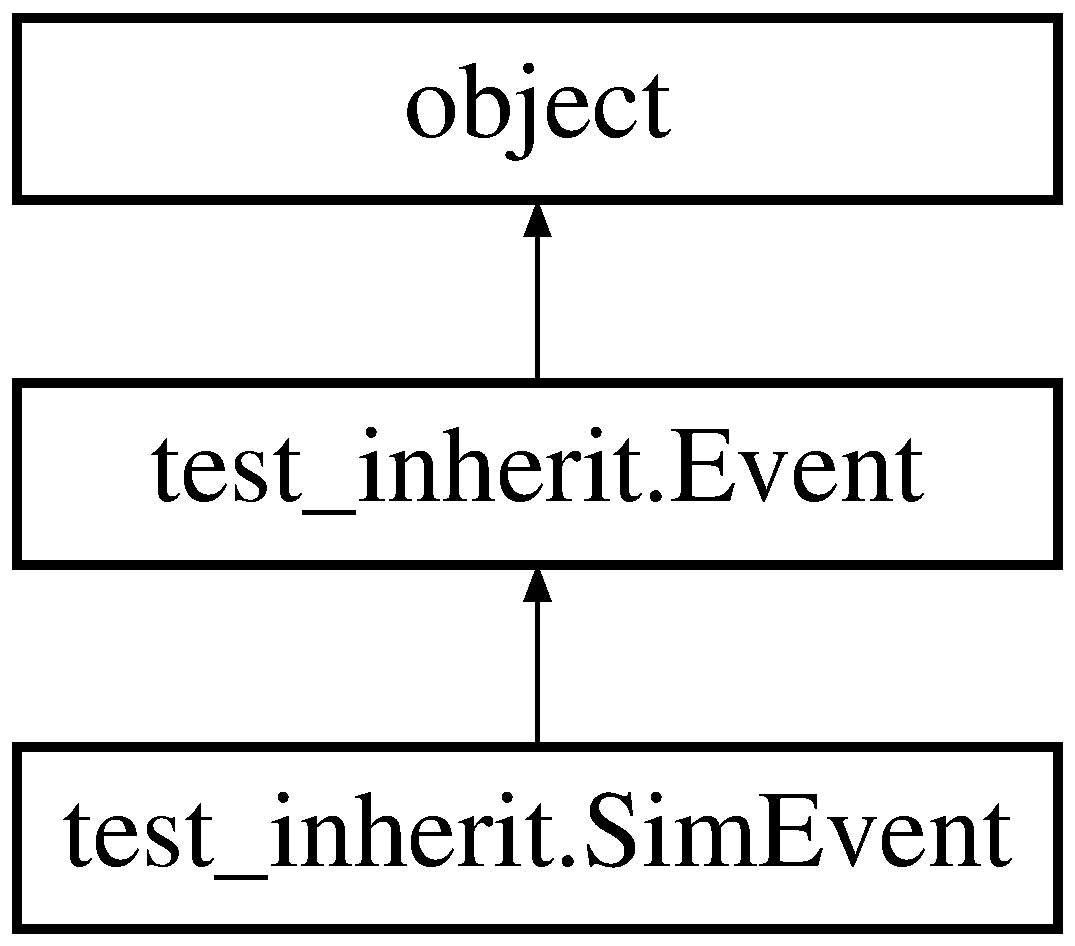
\includegraphics[height=3.000000cm]{classtest__inherit_1_1_sim_event}
\end{center}
\end{figure}
\subsection*{Public Member Functions}
\begin{DoxyCompactItemize}
\item 
def \hyperlink{classtest__inherit_1_1_sim_event_ab051508210854a9a81b1345b404acfab}{\-\_\-\-\_\-init\-\_\-\-\_\-}
\item 
def \hyperlink{classtest__inherit_1_1_sim_event_a270fb21de000aca3cb985cac075af503}{datetime}
\end{DoxyCompactItemize}
\subsection*{Public Attributes}
\begin{DoxyCompactItemize}
\item 
\hyperlink{classtest__inherit_1_1_sim_event_a6d566ba250cca6d17e970715706e636c}{datetime}
\end{DoxyCompactItemize}


\subsection{Constructor \& Destructor Documentation}
\hypertarget{classtest__inherit_1_1_sim_event_ab051508210854a9a81b1345b404acfab}{\index{test\-\_\-inherit\-::\-Sim\-Event@{test\-\_\-inherit\-::\-Sim\-Event}!\-\_\-\-\_\-init\-\_\-\-\_\-@{\-\_\-\-\_\-init\-\_\-\-\_\-}}
\index{\-\_\-\-\_\-init\-\_\-\-\_\-@{\-\_\-\-\_\-init\-\_\-\-\_\-}!test_inherit::SimEvent@{test\-\_\-inherit\-::\-Sim\-Event}}
\subsubsection[{\-\_\-\-\_\-init\-\_\-\-\_\-}]{\setlength{\rightskip}{0pt plus 5cm}def test\-\_\-inherit.\-Sim\-Event.\-\_\-\-\_\-init\-\_\-\-\_\- (
\begin{DoxyParamCaption}
\item[{}]{self, }
\item[{}]{stream, }
\item[{}]{id, }
\item[{}]{rev, }
\item[{}]{config}
\end{DoxyParamCaption}
)}}\label{classtest__inherit_1_1_sim_event_ab051508210854a9a81b1345b404acfab}


\subsection{Member Function Documentation}
\hypertarget{classtest__inherit_1_1_sim_event_a270fb21de000aca3cb985cac075af503}{\index{test\-\_\-inherit\-::\-Sim\-Event@{test\-\_\-inherit\-::\-Sim\-Event}!datetime@{datetime}}
\index{datetime@{datetime}!test_inherit::SimEvent@{test\-\_\-inherit\-::\-Sim\-Event}}
\subsubsection[{datetime}]{\setlength{\rightskip}{0pt plus 5cm}def test\-\_\-inherit.\-Sim\-Event.\-datetime (
\begin{DoxyParamCaption}
\item[{}]{self, }
\item[{}]{value}
\end{DoxyParamCaption}
)}}\label{classtest__inherit_1_1_sim_event_a270fb21de000aca3cb985cac075af503}


\subsection{Member Data Documentation}
\hypertarget{classtest__inherit_1_1_sim_event_a6d566ba250cca6d17e970715706e636c}{\index{test\-\_\-inherit\-::\-Sim\-Event@{test\-\_\-inherit\-::\-Sim\-Event}!datetime@{datetime}}
\index{datetime@{datetime}!test_inherit::SimEvent@{test\-\_\-inherit\-::\-Sim\-Event}}
\subsubsection[{datetime}]{\setlength{\rightskip}{0pt plus 5cm}test\-\_\-inherit.\-Sim\-Event.\-datetime}}\label{classtest__inherit_1_1_sim_event_a6d566ba250cca6d17e970715706e636c}


The documentation for this class was generated from the following file\-:\begin{DoxyCompactItemize}
\item 
amonpy/dev/test/\hyperlink{test__inherit_8py}{test\-\_\-inherit.\-py}\end{DoxyCompactItemize}

\hypertarget{classbasic__sim__old_1_1_sim_event}{\section{basic\-\_\-sim\-\_\-old.\-Sim\-Event Class Reference}
\label{classbasic__sim__old_1_1_sim_event}\index{basic\-\_\-sim\-\_\-old.\-Sim\-Event@{basic\-\_\-sim\-\_\-old.\-Sim\-Event}}
}
Inheritance diagram for basic\-\_\-sim\-\_\-old.\-Sim\-Event\-:\begin{figure}[H]
\begin{center}
\leavevmode
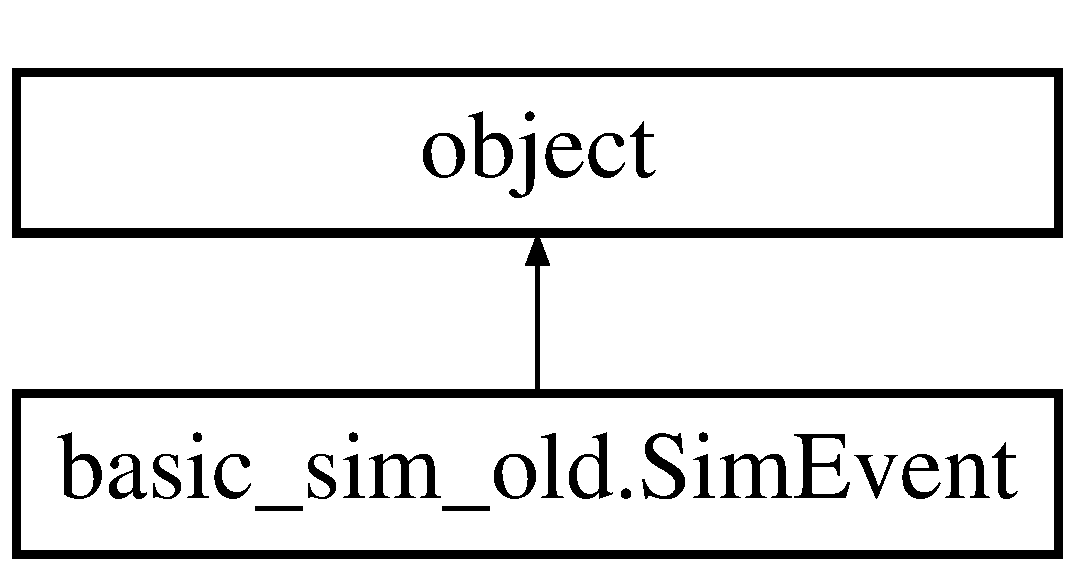
\includegraphics[height=2.000000cm]{classbasic__sim__old_1_1_sim_event}
\end{center}
\end{figure}
\subsection*{Public Member Functions}
\begin{DoxyCompactItemize}
\item 
def \hyperlink{classbasic__sim__old_1_1_sim_event_aaef4bb94745ed59caf2fa4e59aa2b6e7}{\-\_\-\-\_\-init\-\_\-\-\_\-}
\item 
def \hyperlink{classbasic__sim__old_1_1_sim_event_a02262a28ffb04370abf5968353798354}{\-\_\-\-\_\-del\-\_\-\-\_\-}
\item 
def \hyperlink{classbasic__sim__old_1_1_sim_event_a0e06cb1a31ac729d90b219864a1d327f}{forprint}
\item 
def \hyperlink{classbasic__sim__old_1_1_sim_event_ab455dcbf5fd02e68e8f1b670195c161c}{jday}
\item 
def \hyperlink{classbasic__sim__old_1_1_sim_event_ad59c9f8114aa2f50b7d7301204ca7bbc}{G\-S\-T}
\item 
def \hyperlink{classbasic__sim__old_1_1_sim_event_a5b9ea8c6d9ce5a40a28a3a8eee6a3674}{L\-S\-T}
\item 
def \hyperlink{classbasic__sim__old_1_1_sim_event_ad889b1c098f4b32899232212c551dc3f}{Alt\-Az}
\item 
def \hyperlink{classbasic__sim__old_1_1_sim_event_ac4a235942421c942a7824956d86d0276}{Lat\-Lon}
\item 
def \hyperlink{classbasic__sim__old_1_1_sim_event_a9fa90508863fcdd824388fdfbfd167b0}{ra\-Dec}
\item 
def \hyperlink{classbasic__sim__old_1_1_sim_event_ab3768f5029c64a2361813ad845df2f57}{R\-A}
\item 
def \hyperlink{classbasic__sim__old_1_1_sim_event_a1613d4a9fc11172d53dcfed4a37278af}{dec}
\end{DoxyCompactItemize}
\subsection*{Public Attributes}
\begin{DoxyCompactItemize}
\item 
\hyperlink{classbasic__sim__old_1_1_sim_event_ac75852235bc1c9636274dbfb52d22394}{stream}
\item 
\hyperlink{classbasic__sim__old_1_1_sim_event_a5c0d91c14f018c2ddd192e6a26767d79}{id}
\item 
\hyperlink{classbasic__sim__old_1_1_sim_event_a6b48b8974f4ef4541bf9c09b7dd7a054}{rev}
\item 
\hyperlink{classbasic__sim__old_1_1_sim_event_adbe3757a4fee40731f878bd411c9a763}{datetime}
\item 
\hyperlink{classbasic__sim__old_1_1_sim_event_a34b942af37c343a76ffb11ec96507ee4}{nevents}
\item 
\hyperlink{classbasic__sim__old_1_1_sim_event_af92dc762c35bd75c05bb8bf6c9616b00}{delta\-T}
\item 
\hyperlink{classbasic__sim__old_1_1_sim_event_afd43199470abde63072e5e91d8217cf7}{sigma\-T}
\item 
\hyperlink{classbasic__sim__old_1_1_sim_event_adabdf127ae2580a06fbc05cf768cf8a6}{false\-\_\-pos}
\item 
\hyperlink{classbasic__sim__old_1_1_sim_event_a3028fb127e8ce49c2275bcf26a7758f0}{pvalue}
\item 
\hyperlink{classbasic__sim__old_1_1_sim_event_a6884bb4ef3a110c576b844ba4c55a2de}{observing}
\item 
\hyperlink{classbasic__sim__old_1_1_sim_event_ad97bf46d023e5e0b3e31471c33476b3a}{trigger}
\item 
\hyperlink{classbasic__sim__old_1_1_sim_event_aa62ee00b9bd61aec1cf8d675e10bcdb1}{type}
\item 
\hyperlink{classbasic__sim__old_1_1_sim_event_a472fbb98ba6f3a6bb174896f23866225}{point\-\_\-\-R\-A}
\item 
\hyperlink{classbasic__sim__old_1_1_sim_event_a208e8a3ab9415076107943511f7540d5}{point\-\_\-dec}
\item 
\hyperlink{classbasic__sim__old_1_1_sim_event_a1c0402df96ecafb9ba8ecb7d6e59f329}{longitude}
\item 
\hyperlink{classbasic__sim__old_1_1_sim_event_a4d9d58c5b1062e326ed76c1fb29f51f7}{latitude}
\item 
\hyperlink{classbasic__sim__old_1_1_sim_event_aa41d3a01bb3d4d36266c8aea073d2940}{sigma\-R}
\item 
\hyperlink{classbasic__sim__old_1_1_sim_event_a6711689c3329b821bd9f55692bd37c3c}{elevation}
\item 
\hyperlink{classbasic__sim__old_1_1_sim_event_a3963adc4a383e33d00e1be986fa37371}{skymap}
\item 
\hyperlink{classbasic__sim__old_1_1_sim_event_abd2b40dbe9eb82436ce686a4e921a262}{az}
\item 
\hyperlink{classbasic__sim__old_1_1_sim_event_a2e0e4bd4058be8f6818604cf8b125bf0}{alt}
\end{DoxyCompactItemize}
\subsection*{Static Public Attributes}
\begin{DoxyCompactItemize}
\item 
int \hyperlink{classbasic__sim__old_1_1_sim_event_a06109f4e9dc7bd1249d8cbbc910c623d}{max\-\_\-streams} = 100
\item 
list \hyperlink{classbasic__sim__old_1_1_sim_event_a7e7f42822946c5534013986c75c7e6fb}{num\-\_\-events} = \mbox{[}0\mbox{]}
\end{DoxyCompactItemize}


\subsection{Constructor \& Destructor Documentation}
\hypertarget{classbasic__sim__old_1_1_sim_event_aaef4bb94745ed59caf2fa4e59aa2b6e7}{\index{basic\-\_\-sim\-\_\-old\-::\-Sim\-Event@{basic\-\_\-sim\-\_\-old\-::\-Sim\-Event}!\-\_\-\-\_\-init\-\_\-\-\_\-@{\-\_\-\-\_\-init\-\_\-\-\_\-}}
\index{\-\_\-\-\_\-init\-\_\-\-\_\-@{\-\_\-\-\_\-init\-\_\-\-\_\-}!basic_sim_old::SimEvent@{basic\-\_\-sim\-\_\-old\-::\-Sim\-Event}}
\subsubsection[{\-\_\-\-\_\-init\-\_\-\-\_\-}]{\setlength{\rightskip}{0pt plus 5cm}def basic\-\_\-sim\-\_\-old.\-Sim\-Event.\-\_\-\-\_\-init\-\_\-\-\_\- (
\begin{DoxyParamCaption}
\item[{}]{self, }
\item[{}]{config}
\end{DoxyParamCaption}
)}}\label{classbasic__sim__old_1_1_sim_event_aaef4bb94745ed59caf2fa4e59aa2b6e7}
\hypertarget{classbasic__sim__old_1_1_sim_event_a02262a28ffb04370abf5968353798354}{\index{basic\-\_\-sim\-\_\-old\-::\-Sim\-Event@{basic\-\_\-sim\-\_\-old\-::\-Sim\-Event}!\-\_\-\-\_\-del\-\_\-\-\_\-@{\-\_\-\-\_\-del\-\_\-\-\_\-}}
\index{\-\_\-\-\_\-del\-\_\-\-\_\-@{\-\_\-\-\_\-del\-\_\-\-\_\-}!basic_sim_old::SimEvent@{basic\-\_\-sim\-\_\-old\-::\-Sim\-Event}}
\subsubsection[{\-\_\-\-\_\-del\-\_\-\-\_\-}]{\setlength{\rightskip}{0pt plus 5cm}def basic\-\_\-sim\-\_\-old.\-Sim\-Event.\-\_\-\-\_\-del\-\_\-\-\_\- (
\begin{DoxyParamCaption}
\item[{}]{self}
\end{DoxyParamCaption}
)}}\label{classbasic__sim__old_1_1_sim_event_a02262a28ffb04370abf5968353798354}


\subsection{Member Function Documentation}
\hypertarget{classbasic__sim__old_1_1_sim_event_ad889b1c098f4b32899232212c551dc3f}{\index{basic\-\_\-sim\-\_\-old\-::\-Sim\-Event@{basic\-\_\-sim\-\_\-old\-::\-Sim\-Event}!Alt\-Az@{Alt\-Az}}
\index{Alt\-Az@{Alt\-Az}!basic_sim_old::SimEvent@{basic\-\_\-sim\-\_\-old\-::\-Sim\-Event}}
\subsubsection[{Alt\-Az}]{\setlength{\rightskip}{0pt plus 5cm}def basic\-\_\-sim\-\_\-old.\-Sim\-Event.\-Alt\-Az (
\begin{DoxyParamCaption}
\item[{}]{self}
\end{DoxyParamCaption}
)}}\label{classbasic__sim__old_1_1_sim_event_ad889b1c098f4b32899232212c551dc3f}
\hypertarget{classbasic__sim__old_1_1_sim_event_a1613d4a9fc11172d53dcfed4a37278af}{\index{basic\-\_\-sim\-\_\-old\-::\-Sim\-Event@{basic\-\_\-sim\-\_\-old\-::\-Sim\-Event}!dec@{dec}}
\index{dec@{dec}!basic_sim_old::SimEvent@{basic\-\_\-sim\-\_\-old\-::\-Sim\-Event}}
\subsubsection[{dec}]{\setlength{\rightskip}{0pt plus 5cm}def basic\-\_\-sim\-\_\-old.\-Sim\-Event.\-dec (
\begin{DoxyParamCaption}
\item[{}]{self}
\end{DoxyParamCaption}
)}}\label{classbasic__sim__old_1_1_sim_event_a1613d4a9fc11172d53dcfed4a37278af}
\hypertarget{classbasic__sim__old_1_1_sim_event_a0e06cb1a31ac729d90b219864a1d327f}{\index{basic\-\_\-sim\-\_\-old\-::\-Sim\-Event@{basic\-\_\-sim\-\_\-old\-::\-Sim\-Event}!forprint@{forprint}}
\index{forprint@{forprint}!basic_sim_old::SimEvent@{basic\-\_\-sim\-\_\-old\-::\-Sim\-Event}}
\subsubsection[{forprint}]{\setlength{\rightskip}{0pt plus 5cm}def basic\-\_\-sim\-\_\-old.\-Sim\-Event.\-forprint (
\begin{DoxyParamCaption}
\item[{}]{self}
\end{DoxyParamCaption}
)}}\label{classbasic__sim__old_1_1_sim_event_a0e06cb1a31ac729d90b219864a1d327f}
\hypertarget{classbasic__sim__old_1_1_sim_event_ad59c9f8114aa2f50b7d7301204ca7bbc}{\index{basic\-\_\-sim\-\_\-old\-::\-Sim\-Event@{basic\-\_\-sim\-\_\-old\-::\-Sim\-Event}!G\-S\-T@{G\-S\-T}}
\index{G\-S\-T@{G\-S\-T}!basic_sim_old::SimEvent@{basic\-\_\-sim\-\_\-old\-::\-Sim\-Event}}
\subsubsection[{G\-S\-T}]{\setlength{\rightskip}{0pt plus 5cm}def basic\-\_\-sim\-\_\-old.\-Sim\-Event.\-G\-S\-T (
\begin{DoxyParamCaption}
\item[{}]{self}
\end{DoxyParamCaption}
)}}\label{classbasic__sim__old_1_1_sim_event_ad59c9f8114aa2f50b7d7301204ca7bbc}
\hypertarget{classbasic__sim__old_1_1_sim_event_ab455dcbf5fd02e68e8f1b670195c161c}{\index{basic\-\_\-sim\-\_\-old\-::\-Sim\-Event@{basic\-\_\-sim\-\_\-old\-::\-Sim\-Event}!jday@{jday}}
\index{jday@{jday}!basic_sim_old::SimEvent@{basic\-\_\-sim\-\_\-old\-::\-Sim\-Event}}
\subsubsection[{jday}]{\setlength{\rightskip}{0pt plus 5cm}def basic\-\_\-sim\-\_\-old.\-Sim\-Event.\-jday (
\begin{DoxyParamCaption}
\item[{}]{self}
\end{DoxyParamCaption}
)}}\label{classbasic__sim__old_1_1_sim_event_ab455dcbf5fd02e68e8f1b670195c161c}
\hypertarget{classbasic__sim__old_1_1_sim_event_ac4a235942421c942a7824956d86d0276}{\index{basic\-\_\-sim\-\_\-old\-::\-Sim\-Event@{basic\-\_\-sim\-\_\-old\-::\-Sim\-Event}!Lat\-Lon@{Lat\-Lon}}
\index{Lat\-Lon@{Lat\-Lon}!basic_sim_old::SimEvent@{basic\-\_\-sim\-\_\-old\-::\-Sim\-Event}}
\subsubsection[{Lat\-Lon}]{\setlength{\rightskip}{0pt plus 5cm}def basic\-\_\-sim\-\_\-old.\-Sim\-Event.\-Lat\-Lon (
\begin{DoxyParamCaption}
\item[{}]{self}
\end{DoxyParamCaption}
)}}\label{classbasic__sim__old_1_1_sim_event_ac4a235942421c942a7824956d86d0276}
\hypertarget{classbasic__sim__old_1_1_sim_event_a5b9ea8c6d9ce5a40a28a3a8eee6a3674}{\index{basic\-\_\-sim\-\_\-old\-::\-Sim\-Event@{basic\-\_\-sim\-\_\-old\-::\-Sim\-Event}!L\-S\-T@{L\-S\-T}}
\index{L\-S\-T@{L\-S\-T}!basic_sim_old::SimEvent@{basic\-\_\-sim\-\_\-old\-::\-Sim\-Event}}
\subsubsection[{L\-S\-T}]{\setlength{\rightskip}{0pt plus 5cm}def basic\-\_\-sim\-\_\-old.\-Sim\-Event.\-L\-S\-T (
\begin{DoxyParamCaption}
\item[{}]{self}
\end{DoxyParamCaption}
)}}\label{classbasic__sim__old_1_1_sim_event_a5b9ea8c6d9ce5a40a28a3a8eee6a3674}
\hypertarget{classbasic__sim__old_1_1_sim_event_ab3768f5029c64a2361813ad845df2f57}{\index{basic\-\_\-sim\-\_\-old\-::\-Sim\-Event@{basic\-\_\-sim\-\_\-old\-::\-Sim\-Event}!R\-A@{R\-A}}
\index{R\-A@{R\-A}!basic_sim_old::SimEvent@{basic\-\_\-sim\-\_\-old\-::\-Sim\-Event}}
\subsubsection[{R\-A}]{\setlength{\rightskip}{0pt plus 5cm}def basic\-\_\-sim\-\_\-old.\-Sim\-Event.\-R\-A (
\begin{DoxyParamCaption}
\item[{}]{self}
\end{DoxyParamCaption}
)}}\label{classbasic__sim__old_1_1_sim_event_ab3768f5029c64a2361813ad845df2f57}
\hypertarget{classbasic__sim__old_1_1_sim_event_a9fa90508863fcdd824388fdfbfd167b0}{\index{basic\-\_\-sim\-\_\-old\-::\-Sim\-Event@{basic\-\_\-sim\-\_\-old\-::\-Sim\-Event}!ra\-Dec@{ra\-Dec}}
\index{ra\-Dec@{ra\-Dec}!basic_sim_old::SimEvent@{basic\-\_\-sim\-\_\-old\-::\-Sim\-Event}}
\subsubsection[{ra\-Dec}]{\setlength{\rightskip}{0pt plus 5cm}def basic\-\_\-sim\-\_\-old.\-Sim\-Event.\-ra\-Dec (
\begin{DoxyParamCaption}
\item[{}]{self}
\end{DoxyParamCaption}
)}}\label{classbasic__sim__old_1_1_sim_event_a9fa90508863fcdd824388fdfbfd167b0}


\subsection{Member Data Documentation}
\hypertarget{classbasic__sim__old_1_1_sim_event_a2e0e4bd4058be8f6818604cf8b125bf0}{\index{basic\-\_\-sim\-\_\-old\-::\-Sim\-Event@{basic\-\_\-sim\-\_\-old\-::\-Sim\-Event}!alt@{alt}}
\index{alt@{alt}!basic_sim_old::SimEvent@{basic\-\_\-sim\-\_\-old\-::\-Sim\-Event}}
\subsubsection[{alt}]{\setlength{\rightskip}{0pt plus 5cm}basic\-\_\-sim\-\_\-old.\-Sim\-Event.\-alt}}\label{classbasic__sim__old_1_1_sim_event_a2e0e4bd4058be8f6818604cf8b125bf0}
\hypertarget{classbasic__sim__old_1_1_sim_event_abd2b40dbe9eb82436ce686a4e921a262}{\index{basic\-\_\-sim\-\_\-old\-::\-Sim\-Event@{basic\-\_\-sim\-\_\-old\-::\-Sim\-Event}!az@{az}}
\index{az@{az}!basic_sim_old::SimEvent@{basic\-\_\-sim\-\_\-old\-::\-Sim\-Event}}
\subsubsection[{az}]{\setlength{\rightskip}{0pt plus 5cm}basic\-\_\-sim\-\_\-old.\-Sim\-Event.\-az}}\label{classbasic__sim__old_1_1_sim_event_abd2b40dbe9eb82436ce686a4e921a262}
\hypertarget{classbasic__sim__old_1_1_sim_event_adbe3757a4fee40731f878bd411c9a763}{\index{basic\-\_\-sim\-\_\-old\-::\-Sim\-Event@{basic\-\_\-sim\-\_\-old\-::\-Sim\-Event}!datetime@{datetime}}
\index{datetime@{datetime}!basic_sim_old::SimEvent@{basic\-\_\-sim\-\_\-old\-::\-Sim\-Event}}
\subsubsection[{datetime}]{\setlength{\rightskip}{0pt plus 5cm}basic\-\_\-sim\-\_\-old.\-Sim\-Event.\-datetime}}\label{classbasic__sim__old_1_1_sim_event_adbe3757a4fee40731f878bd411c9a763}
\hypertarget{classbasic__sim__old_1_1_sim_event_af92dc762c35bd75c05bb8bf6c9616b00}{\index{basic\-\_\-sim\-\_\-old\-::\-Sim\-Event@{basic\-\_\-sim\-\_\-old\-::\-Sim\-Event}!delta\-T@{delta\-T}}
\index{delta\-T@{delta\-T}!basic_sim_old::SimEvent@{basic\-\_\-sim\-\_\-old\-::\-Sim\-Event}}
\subsubsection[{delta\-T}]{\setlength{\rightskip}{0pt plus 5cm}basic\-\_\-sim\-\_\-old.\-Sim\-Event.\-delta\-T}}\label{classbasic__sim__old_1_1_sim_event_af92dc762c35bd75c05bb8bf6c9616b00}
\hypertarget{classbasic__sim__old_1_1_sim_event_a6711689c3329b821bd9f55692bd37c3c}{\index{basic\-\_\-sim\-\_\-old\-::\-Sim\-Event@{basic\-\_\-sim\-\_\-old\-::\-Sim\-Event}!elevation@{elevation}}
\index{elevation@{elevation}!basic_sim_old::SimEvent@{basic\-\_\-sim\-\_\-old\-::\-Sim\-Event}}
\subsubsection[{elevation}]{\setlength{\rightskip}{0pt plus 5cm}basic\-\_\-sim\-\_\-old.\-Sim\-Event.\-elevation}}\label{classbasic__sim__old_1_1_sim_event_a6711689c3329b821bd9f55692bd37c3c}
\hypertarget{classbasic__sim__old_1_1_sim_event_adabdf127ae2580a06fbc05cf768cf8a6}{\index{basic\-\_\-sim\-\_\-old\-::\-Sim\-Event@{basic\-\_\-sim\-\_\-old\-::\-Sim\-Event}!false\-\_\-pos@{false\-\_\-pos}}
\index{false\-\_\-pos@{false\-\_\-pos}!basic_sim_old::SimEvent@{basic\-\_\-sim\-\_\-old\-::\-Sim\-Event}}
\subsubsection[{false\-\_\-pos}]{\setlength{\rightskip}{0pt plus 5cm}basic\-\_\-sim\-\_\-old.\-Sim\-Event.\-false\-\_\-pos}}\label{classbasic__sim__old_1_1_sim_event_adabdf127ae2580a06fbc05cf768cf8a6}
\hypertarget{classbasic__sim__old_1_1_sim_event_a5c0d91c14f018c2ddd192e6a26767d79}{\index{basic\-\_\-sim\-\_\-old\-::\-Sim\-Event@{basic\-\_\-sim\-\_\-old\-::\-Sim\-Event}!id@{id}}
\index{id@{id}!basic_sim_old::SimEvent@{basic\-\_\-sim\-\_\-old\-::\-Sim\-Event}}
\subsubsection[{id}]{\setlength{\rightskip}{0pt plus 5cm}basic\-\_\-sim\-\_\-old.\-Sim\-Event.\-id}}\label{classbasic__sim__old_1_1_sim_event_a5c0d91c14f018c2ddd192e6a26767d79}
\hypertarget{classbasic__sim__old_1_1_sim_event_a4d9d58c5b1062e326ed76c1fb29f51f7}{\index{basic\-\_\-sim\-\_\-old\-::\-Sim\-Event@{basic\-\_\-sim\-\_\-old\-::\-Sim\-Event}!latitude@{latitude}}
\index{latitude@{latitude}!basic_sim_old::SimEvent@{basic\-\_\-sim\-\_\-old\-::\-Sim\-Event}}
\subsubsection[{latitude}]{\setlength{\rightskip}{0pt plus 5cm}basic\-\_\-sim\-\_\-old.\-Sim\-Event.\-latitude}}\label{classbasic__sim__old_1_1_sim_event_a4d9d58c5b1062e326ed76c1fb29f51f7}
\hypertarget{classbasic__sim__old_1_1_sim_event_a1c0402df96ecafb9ba8ecb7d6e59f329}{\index{basic\-\_\-sim\-\_\-old\-::\-Sim\-Event@{basic\-\_\-sim\-\_\-old\-::\-Sim\-Event}!longitude@{longitude}}
\index{longitude@{longitude}!basic_sim_old::SimEvent@{basic\-\_\-sim\-\_\-old\-::\-Sim\-Event}}
\subsubsection[{longitude}]{\setlength{\rightskip}{0pt plus 5cm}basic\-\_\-sim\-\_\-old.\-Sim\-Event.\-longitude}}\label{classbasic__sim__old_1_1_sim_event_a1c0402df96ecafb9ba8ecb7d6e59f329}
\hypertarget{classbasic__sim__old_1_1_sim_event_a06109f4e9dc7bd1249d8cbbc910c623d}{\index{basic\-\_\-sim\-\_\-old\-::\-Sim\-Event@{basic\-\_\-sim\-\_\-old\-::\-Sim\-Event}!max\-\_\-streams@{max\-\_\-streams}}
\index{max\-\_\-streams@{max\-\_\-streams}!basic_sim_old::SimEvent@{basic\-\_\-sim\-\_\-old\-::\-Sim\-Event}}
\subsubsection[{max\-\_\-streams}]{\setlength{\rightskip}{0pt plus 5cm}int basic\-\_\-sim\-\_\-old.\-Sim\-Event.\-max\-\_\-streams = 100\hspace{0.3cm}{\ttfamily [static]}}}\label{classbasic__sim__old_1_1_sim_event_a06109f4e9dc7bd1249d8cbbc910c623d}
\hypertarget{classbasic__sim__old_1_1_sim_event_a34b942af37c343a76ffb11ec96507ee4}{\index{basic\-\_\-sim\-\_\-old\-::\-Sim\-Event@{basic\-\_\-sim\-\_\-old\-::\-Sim\-Event}!nevents@{nevents}}
\index{nevents@{nevents}!basic_sim_old::SimEvent@{basic\-\_\-sim\-\_\-old\-::\-Sim\-Event}}
\subsubsection[{nevents}]{\setlength{\rightskip}{0pt plus 5cm}basic\-\_\-sim\-\_\-old.\-Sim\-Event.\-nevents}}\label{classbasic__sim__old_1_1_sim_event_a34b942af37c343a76ffb11ec96507ee4}
\hypertarget{classbasic__sim__old_1_1_sim_event_a7e7f42822946c5534013986c75c7e6fb}{\index{basic\-\_\-sim\-\_\-old\-::\-Sim\-Event@{basic\-\_\-sim\-\_\-old\-::\-Sim\-Event}!num\-\_\-events@{num\-\_\-events}}
\index{num\-\_\-events@{num\-\_\-events}!basic_sim_old::SimEvent@{basic\-\_\-sim\-\_\-old\-::\-Sim\-Event}}
\subsubsection[{num\-\_\-events}]{\setlength{\rightskip}{0pt plus 5cm}list basic\-\_\-sim\-\_\-old.\-Sim\-Event.\-num\-\_\-events = \mbox{[}0\mbox{]}\hspace{0.3cm}{\ttfamily [static]}}}\label{classbasic__sim__old_1_1_sim_event_a7e7f42822946c5534013986c75c7e6fb}
\hypertarget{classbasic__sim__old_1_1_sim_event_a6884bb4ef3a110c576b844ba4c55a2de}{\index{basic\-\_\-sim\-\_\-old\-::\-Sim\-Event@{basic\-\_\-sim\-\_\-old\-::\-Sim\-Event}!observing@{observing}}
\index{observing@{observing}!basic_sim_old::SimEvent@{basic\-\_\-sim\-\_\-old\-::\-Sim\-Event}}
\subsubsection[{observing}]{\setlength{\rightskip}{0pt plus 5cm}basic\-\_\-sim\-\_\-old.\-Sim\-Event.\-observing}}\label{classbasic__sim__old_1_1_sim_event_a6884bb4ef3a110c576b844ba4c55a2de}
\hypertarget{classbasic__sim__old_1_1_sim_event_a208e8a3ab9415076107943511f7540d5}{\index{basic\-\_\-sim\-\_\-old\-::\-Sim\-Event@{basic\-\_\-sim\-\_\-old\-::\-Sim\-Event}!point\-\_\-dec@{point\-\_\-dec}}
\index{point\-\_\-dec@{point\-\_\-dec}!basic_sim_old::SimEvent@{basic\-\_\-sim\-\_\-old\-::\-Sim\-Event}}
\subsubsection[{point\-\_\-dec}]{\setlength{\rightskip}{0pt plus 5cm}basic\-\_\-sim\-\_\-old.\-Sim\-Event.\-point\-\_\-dec}}\label{classbasic__sim__old_1_1_sim_event_a208e8a3ab9415076107943511f7540d5}
\hypertarget{classbasic__sim__old_1_1_sim_event_a472fbb98ba6f3a6bb174896f23866225}{\index{basic\-\_\-sim\-\_\-old\-::\-Sim\-Event@{basic\-\_\-sim\-\_\-old\-::\-Sim\-Event}!point\-\_\-\-R\-A@{point\-\_\-\-R\-A}}
\index{point\-\_\-\-R\-A@{point\-\_\-\-R\-A}!basic_sim_old::SimEvent@{basic\-\_\-sim\-\_\-old\-::\-Sim\-Event}}
\subsubsection[{point\-\_\-\-R\-A}]{\setlength{\rightskip}{0pt plus 5cm}basic\-\_\-sim\-\_\-old.\-Sim\-Event.\-point\-\_\-\-R\-A}}\label{classbasic__sim__old_1_1_sim_event_a472fbb98ba6f3a6bb174896f23866225}
\hypertarget{classbasic__sim__old_1_1_sim_event_a3028fb127e8ce49c2275bcf26a7758f0}{\index{basic\-\_\-sim\-\_\-old\-::\-Sim\-Event@{basic\-\_\-sim\-\_\-old\-::\-Sim\-Event}!pvalue@{pvalue}}
\index{pvalue@{pvalue}!basic_sim_old::SimEvent@{basic\-\_\-sim\-\_\-old\-::\-Sim\-Event}}
\subsubsection[{pvalue}]{\setlength{\rightskip}{0pt plus 5cm}basic\-\_\-sim\-\_\-old.\-Sim\-Event.\-pvalue}}\label{classbasic__sim__old_1_1_sim_event_a3028fb127e8ce49c2275bcf26a7758f0}
\hypertarget{classbasic__sim__old_1_1_sim_event_a6b48b8974f4ef4541bf9c09b7dd7a054}{\index{basic\-\_\-sim\-\_\-old\-::\-Sim\-Event@{basic\-\_\-sim\-\_\-old\-::\-Sim\-Event}!rev@{rev}}
\index{rev@{rev}!basic_sim_old::SimEvent@{basic\-\_\-sim\-\_\-old\-::\-Sim\-Event}}
\subsubsection[{rev}]{\setlength{\rightskip}{0pt plus 5cm}basic\-\_\-sim\-\_\-old.\-Sim\-Event.\-rev}}\label{classbasic__sim__old_1_1_sim_event_a6b48b8974f4ef4541bf9c09b7dd7a054}
\hypertarget{classbasic__sim__old_1_1_sim_event_aa41d3a01bb3d4d36266c8aea073d2940}{\index{basic\-\_\-sim\-\_\-old\-::\-Sim\-Event@{basic\-\_\-sim\-\_\-old\-::\-Sim\-Event}!sigma\-R@{sigma\-R}}
\index{sigma\-R@{sigma\-R}!basic_sim_old::SimEvent@{basic\-\_\-sim\-\_\-old\-::\-Sim\-Event}}
\subsubsection[{sigma\-R}]{\setlength{\rightskip}{0pt plus 5cm}basic\-\_\-sim\-\_\-old.\-Sim\-Event.\-sigma\-R}}\label{classbasic__sim__old_1_1_sim_event_aa41d3a01bb3d4d36266c8aea073d2940}
\hypertarget{classbasic__sim__old_1_1_sim_event_afd43199470abde63072e5e91d8217cf7}{\index{basic\-\_\-sim\-\_\-old\-::\-Sim\-Event@{basic\-\_\-sim\-\_\-old\-::\-Sim\-Event}!sigma\-T@{sigma\-T}}
\index{sigma\-T@{sigma\-T}!basic_sim_old::SimEvent@{basic\-\_\-sim\-\_\-old\-::\-Sim\-Event}}
\subsubsection[{sigma\-T}]{\setlength{\rightskip}{0pt plus 5cm}basic\-\_\-sim\-\_\-old.\-Sim\-Event.\-sigma\-T}}\label{classbasic__sim__old_1_1_sim_event_afd43199470abde63072e5e91d8217cf7}
\hypertarget{classbasic__sim__old_1_1_sim_event_a3963adc4a383e33d00e1be986fa37371}{\index{basic\-\_\-sim\-\_\-old\-::\-Sim\-Event@{basic\-\_\-sim\-\_\-old\-::\-Sim\-Event}!skymap@{skymap}}
\index{skymap@{skymap}!basic_sim_old::SimEvent@{basic\-\_\-sim\-\_\-old\-::\-Sim\-Event}}
\subsubsection[{skymap}]{\setlength{\rightskip}{0pt plus 5cm}basic\-\_\-sim\-\_\-old.\-Sim\-Event.\-skymap}}\label{classbasic__sim__old_1_1_sim_event_a3963adc4a383e33d00e1be986fa37371}
\hypertarget{classbasic__sim__old_1_1_sim_event_ac75852235bc1c9636274dbfb52d22394}{\index{basic\-\_\-sim\-\_\-old\-::\-Sim\-Event@{basic\-\_\-sim\-\_\-old\-::\-Sim\-Event}!stream@{stream}}
\index{stream@{stream}!basic_sim_old::SimEvent@{basic\-\_\-sim\-\_\-old\-::\-Sim\-Event}}
\subsubsection[{stream}]{\setlength{\rightskip}{0pt plus 5cm}basic\-\_\-sim\-\_\-old.\-Sim\-Event.\-stream}}\label{classbasic__sim__old_1_1_sim_event_ac75852235bc1c9636274dbfb52d22394}
\hypertarget{classbasic__sim__old_1_1_sim_event_ad97bf46d023e5e0b3e31471c33476b3a}{\index{basic\-\_\-sim\-\_\-old\-::\-Sim\-Event@{basic\-\_\-sim\-\_\-old\-::\-Sim\-Event}!trigger@{trigger}}
\index{trigger@{trigger}!basic_sim_old::SimEvent@{basic\-\_\-sim\-\_\-old\-::\-Sim\-Event}}
\subsubsection[{trigger}]{\setlength{\rightskip}{0pt plus 5cm}basic\-\_\-sim\-\_\-old.\-Sim\-Event.\-trigger}}\label{classbasic__sim__old_1_1_sim_event_ad97bf46d023e5e0b3e31471c33476b3a}
\hypertarget{classbasic__sim__old_1_1_sim_event_aa62ee00b9bd61aec1cf8d675e10bcdb1}{\index{basic\-\_\-sim\-\_\-old\-::\-Sim\-Event@{basic\-\_\-sim\-\_\-old\-::\-Sim\-Event}!type@{type}}
\index{type@{type}!basic_sim_old::SimEvent@{basic\-\_\-sim\-\_\-old\-::\-Sim\-Event}}
\subsubsection[{type}]{\setlength{\rightskip}{0pt plus 5cm}basic\-\_\-sim\-\_\-old.\-Sim\-Event.\-type}}\label{classbasic__sim__old_1_1_sim_event_aa62ee00b9bd61aec1cf8d675e10bcdb1}


The documentation for this class was generated from the following file\-:\begin{DoxyCompactItemize}
\item 
amonpy/dev/test/\hyperlink{basic__sim__old_8py}{basic\-\_\-sim\-\_\-old.\-py}\end{DoxyCompactItemize}

\hypertarget{classgrbsim_1_1_source}{\section{grbsim.\-Source Class Reference}
\label{classgrbsim_1_1_source}\index{grbsim.\-Source@{grbsim.\-Source}}
}
Inheritance diagram for grbsim.\-Source\-:\begin{figure}[H]
\begin{center}
\leavevmode
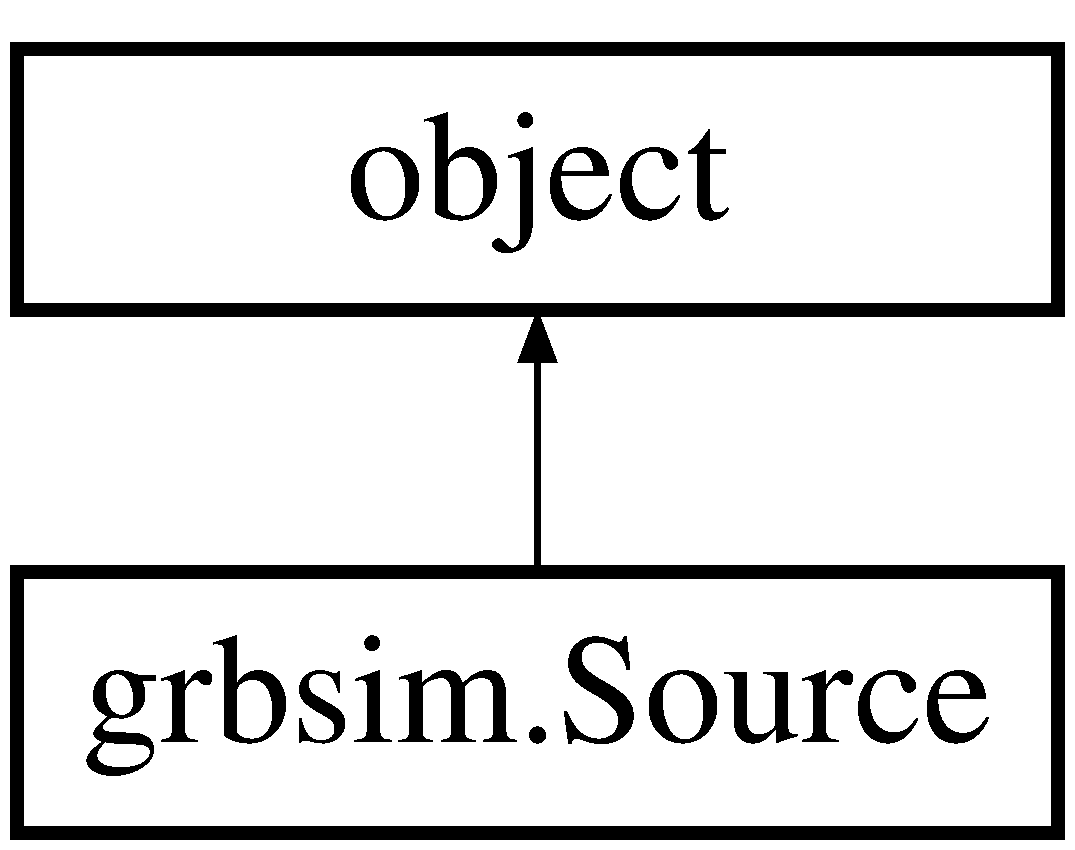
\includegraphics[height=2.000000cm]{dd/d6f/classgrbsim_1_1_source}
\end{center}
\end{figure}
\subsection*{Public Member Functions}
\begin{DoxyCompactItemize}
\item 
def \hyperlink{classgrbsim_1_1_source_a6e483581eeabd09848f71dcdfb46a7bb}{\-\_\-\-\_\-init\-\_\-\-\_\-}
\item 
def \hyperlink{classgrbsim_1_1_source_ad56402a366d30bde07effb65c0645195}{L}
\item 
def \hyperlink{classgrbsim_1_1_source_abc5ca7a3ed742374da80d0cb60aad138}{zsim}
\item 
def \hyperlink{classgrbsim_1_1_source_a412a8b90423af5e02d62aeea10d896d8}{log\-Lsim}
\item 
def \hyperlink{classgrbsim_1_1_source_a0bf9a498b93dfa540547f658e5b4a631}{D\-\_\-\-L}
\item 
def \hyperlink{classgrbsim_1_1_source_a408e7cbd2964af597e37b8cce0934e3e}{Eflux}
\item 
def \hyperlink{classgrbsim_1_1_source_aa9e49ab85c24a8d50825fd733c6c16c9}{Nflux}
\end{DoxyCompactItemize}
\subsection*{Public Attributes}
\begin{DoxyCompactItemize}
\item 
\hyperlink{classgrbsim_1_1_source_a40756599695386befd7d94dea7c45c67}{P}
\item 
\hyperlink{classgrbsim_1_1_source_aa8feb6cf28391b9206c57f0b5ea1dd2a}{spec}
\item 
\hyperlink{classgrbsim_1_1_source_aa983a728c20508521a6e442d8692802a}{z}
\item 
\hyperlink{classgrbsim_1_1_source_a1c36aeb1b0caa2b1c72b1d9536e04999}{log\-L}
\item 
\hyperlink{classgrbsim_1_1_source_a49ad1adc6c791d565301090c86734bd3}{ztrials}
\item 
\hyperlink{classgrbsim_1_1_source_a80a43f13cc9341bb425fc1e29c799a79}{Ltrials}
\end{DoxyCompactItemize}


\subsection{Detailed Description}


Definition at line 167 of file grbsim.\-py.



\subsection{Constructor \& Destructor Documentation}
\hypertarget{classgrbsim_1_1_source_a6e483581eeabd09848f71dcdfb46a7bb}{\index{grbsim\-::\-Source@{grbsim\-::\-Source}!\-\_\-\-\_\-init\-\_\-\-\_\-@{\-\_\-\-\_\-init\-\_\-\-\_\-}}
\index{\-\_\-\-\_\-init\-\_\-\-\_\-@{\-\_\-\-\_\-init\-\_\-\-\_\-}!grbsim::Source@{grbsim\-::\-Source}}
\subsubsection[{\-\_\-\-\_\-init\-\_\-\-\_\-}]{\setlength{\rightskip}{0pt plus 5cm}def grbsim.\-Source.\-\_\-\-\_\-init\-\_\-\-\_\- (
\begin{DoxyParamCaption}
\item[{}]{self, }
\item[{}]{z, }
\item[{}]{P, }
\item[{}]{spec}
\end{DoxyParamCaption}
)}}\label{classgrbsim_1_1_source_a6e483581eeabd09848f71dcdfb46a7bb}


Definition at line 168 of file grbsim.\-py.



\subsection{Member Function Documentation}
\hypertarget{classgrbsim_1_1_source_a0bf9a498b93dfa540547f658e5b4a631}{\index{grbsim\-::\-Source@{grbsim\-::\-Source}!D\-\_\-\-L@{D\-\_\-\-L}}
\index{D\-\_\-\-L@{D\-\_\-\-L}!grbsim::Source@{grbsim\-::\-Source}}
\subsubsection[{D\-\_\-\-L}]{\setlength{\rightskip}{0pt plus 5cm}def grbsim.\-Source.\-D\-\_\-\-L (
\begin{DoxyParamCaption}
\item[{}]{self}
\end{DoxyParamCaption}
)}}\label{classgrbsim_1_1_source_a0bf9a498b93dfa540547f658e5b4a631}


Definition at line 216 of file grbsim.\-py.

\hypertarget{classgrbsim_1_1_source_a408e7cbd2964af597e37b8cce0934e3e}{\index{grbsim\-::\-Source@{grbsim\-::\-Source}!Eflux@{Eflux}}
\index{Eflux@{Eflux}!grbsim::Source@{grbsim\-::\-Source}}
\subsubsection[{Eflux}]{\setlength{\rightskip}{0pt plus 5cm}def grbsim.\-Source.\-Eflux (
\begin{DoxyParamCaption}
\item[{}]{self}
\end{DoxyParamCaption}
)}}\label{classgrbsim_1_1_source_a408e7cbd2964af597e37b8cce0934e3e}


Definition at line 222 of file grbsim.\-py.

\hypertarget{classgrbsim_1_1_source_ad56402a366d30bde07effb65c0645195}{\index{grbsim\-::\-Source@{grbsim\-::\-Source}!L@{L}}
\index{L@{L}!grbsim::Source@{grbsim\-::\-Source}}
\subsubsection[{L}]{\setlength{\rightskip}{0pt plus 5cm}def grbsim.\-Source.\-L (
\begin{DoxyParamCaption}
\item[{}]{self}
\end{DoxyParamCaption}
)}}\label{classgrbsim_1_1_source_ad56402a366d30bde07effb65c0645195}


Definition at line 185 of file grbsim.\-py.

\hypertarget{classgrbsim_1_1_source_a412a8b90423af5e02d62aeea10d896d8}{\index{grbsim\-::\-Source@{grbsim\-::\-Source}!log\-Lsim@{log\-Lsim}}
\index{log\-Lsim@{log\-Lsim}!grbsim::Source@{grbsim\-::\-Source}}
\subsubsection[{log\-Lsim}]{\setlength{\rightskip}{0pt plus 5cm}def grbsim.\-Source.\-log\-Lsim (
\begin{DoxyParamCaption}
\item[{}]{self}
\end{DoxyParamCaption}
)}}\label{classgrbsim_1_1_source_a412a8b90423af5e02d62aeea10d896d8}


Definition at line 202 of file grbsim.\-py.

\hypertarget{classgrbsim_1_1_source_aa9e49ab85c24a8d50825fd733c6c16c9}{\index{grbsim\-::\-Source@{grbsim\-::\-Source}!Nflux@{Nflux}}
\index{Nflux@{Nflux}!grbsim::Source@{grbsim\-::\-Source}}
\subsubsection[{Nflux}]{\setlength{\rightskip}{0pt plus 5cm}def grbsim.\-Source.\-Nflux (
\begin{DoxyParamCaption}
\item[{}]{self}
\end{DoxyParamCaption}
)}}\label{classgrbsim_1_1_source_aa9e49ab85c24a8d50825fd733c6c16c9}


Definition at line 226 of file grbsim.\-py.

\hypertarget{classgrbsim_1_1_source_abc5ca7a3ed742374da80d0cb60aad138}{\index{grbsim\-::\-Source@{grbsim\-::\-Source}!zsim@{zsim}}
\index{zsim@{zsim}!grbsim::Source@{grbsim\-::\-Source}}
\subsubsection[{zsim}]{\setlength{\rightskip}{0pt plus 5cm}def grbsim.\-Source.\-zsim (
\begin{DoxyParamCaption}
\item[{}]{self}
\end{DoxyParamCaption}
)}}\label{classgrbsim_1_1_source_abc5ca7a3ed742374da80d0cb60aad138}


Definition at line 189 of file grbsim.\-py.



\subsection{Member Data Documentation}
\hypertarget{classgrbsim_1_1_source_a1c36aeb1b0caa2b1c72b1d9536e04999}{\index{grbsim\-::\-Source@{grbsim\-::\-Source}!log\-L@{log\-L}}
\index{log\-L@{log\-L}!grbsim::Source@{grbsim\-::\-Source}}
\subsubsection[{log\-L}]{\setlength{\rightskip}{0pt plus 5cm}grbsim.\-Source.\-log\-L}}\label{classgrbsim_1_1_source_a1c36aeb1b0caa2b1c72b1d9536e04999}


Definition at line 179 of file grbsim.\-py.

\hypertarget{classgrbsim_1_1_source_a80a43f13cc9341bb425fc1e29c799a79}{\index{grbsim\-::\-Source@{grbsim\-::\-Source}!Ltrials@{Ltrials}}
\index{Ltrials@{Ltrials}!grbsim::Source@{grbsim\-::\-Source}}
\subsubsection[{Ltrials}]{\setlength{\rightskip}{0pt plus 5cm}grbsim.\-Source.\-Ltrials}}\label{classgrbsim_1_1_source_a80a43f13cc9341bb425fc1e29c799a79}


Definition at line 181 of file grbsim.\-py.

\hypertarget{classgrbsim_1_1_source_a40756599695386befd7d94dea7c45c67}{\index{grbsim\-::\-Source@{grbsim\-::\-Source}!P@{P}}
\index{P@{P}!grbsim::Source@{grbsim\-::\-Source}}
\subsubsection[{P}]{\setlength{\rightskip}{0pt plus 5cm}grbsim.\-Source.\-P}}\label{classgrbsim_1_1_source_a40756599695386befd7d94dea7c45c67}


Definition at line 170 of file grbsim.\-py.

\hypertarget{classgrbsim_1_1_source_aa8feb6cf28391b9206c57f0b5ea1dd2a}{\index{grbsim\-::\-Source@{grbsim\-::\-Source}!spec@{spec}}
\index{spec@{spec}!grbsim::Source@{grbsim\-::\-Source}}
\subsubsection[{spec}]{\setlength{\rightskip}{0pt plus 5cm}grbsim.\-Source.\-spec}}\label{classgrbsim_1_1_source_aa8feb6cf28391b9206c57f0b5ea1dd2a}


Definition at line 171 of file grbsim.\-py.

\hypertarget{classgrbsim_1_1_source_aa983a728c20508521a6e442d8692802a}{\index{grbsim\-::\-Source@{grbsim\-::\-Source}!z@{z}}
\index{z@{z}!grbsim::Source@{grbsim\-::\-Source}}
\subsubsection[{z}]{\setlength{\rightskip}{0pt plus 5cm}grbsim.\-Source.\-z}}\label{classgrbsim_1_1_source_aa983a728c20508521a6e442d8692802a}


Definition at line 178 of file grbsim.\-py.

\hypertarget{classgrbsim_1_1_source_a49ad1adc6c791d565301090c86734bd3}{\index{grbsim\-::\-Source@{grbsim\-::\-Source}!ztrials@{ztrials}}
\index{ztrials@{ztrials}!grbsim::Source@{grbsim\-::\-Source}}
\subsubsection[{ztrials}]{\setlength{\rightskip}{0pt plus 5cm}grbsim.\-Source.\-ztrials}}\label{classgrbsim_1_1_source_a49ad1adc6c791d565301090c86734bd3}


Definition at line 180 of file grbsim.\-py.



The documentation for this class was generated from the following file\-:\begin{DoxyCompactItemize}
\item 
amonpy/sim/sources/\hyperlink{grbsim_8py}{grbsim.\-py}\end{DoxyCompactItemize}

\hypertarget{classgrbsim_1_1_spectrum}{\section{grbsim.\-Spectrum Class Reference}
\label{classgrbsim_1_1_spectrum}\index{grbsim.\-Spectrum@{grbsim.\-Spectrum}}
}
Inheritance diagram for grbsim.\-Spectrum\-:\begin{figure}[H]
\begin{center}
\leavevmode
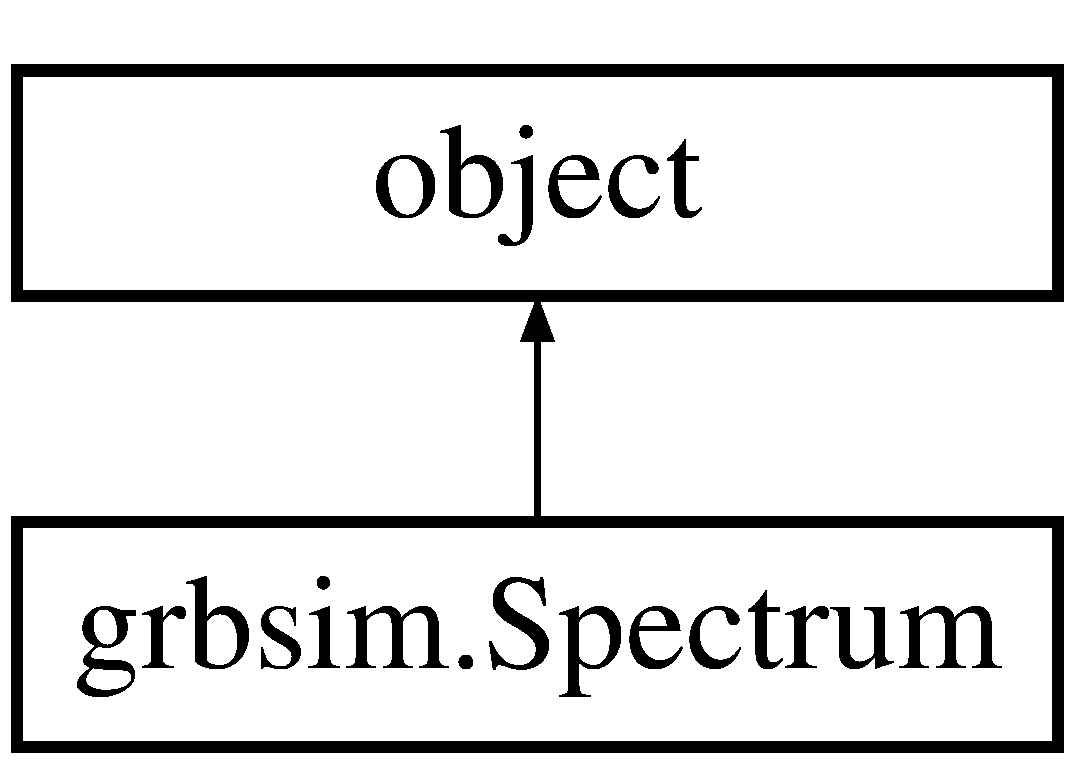
\includegraphics[height=2.000000cm]{dc/d00/classgrbsim_1_1_spectrum}
\end{center}
\end{figure}
\subsection*{Public Member Functions}
\begin{DoxyCompactItemize}
\item 
def \hyperlink{classgrbsim_1_1_spectrum_a0341c6f78c130b7b38216a8bbc187890}{\-\_\-\-\_\-init\-\_\-\-\_\-}
\item 
def \hyperlink{classgrbsim_1_1_spectrum_a23957ee0259fe9a732bcb4ab2c1cfd71}{Ebreak}
\item 
def \hyperlink{classgrbsim_1_1_spectrum_a3e93391e221ca283750d08b8485c9358}{f}
\item 
def \hyperlink{classgrbsim_1_1_spectrum_acf8ca89dded867c619a5dff3189d34c3}{g}
\item 
def \hyperlink{classgrbsim_1_1_spectrum_aa94d37ec5851e690032cc4fe751f8088}{F}
\item 
def \hyperlink{classgrbsim_1_1_spectrum_a3c80da83d9dd35dd221b34ba511350dc}{G}
\item 
def \hyperlink{classgrbsim_1_1_spectrum_ad6edd414e3397c1513b16052e0853afd}{k}
\end{DoxyCompactItemize}
\subsection*{Public Attributes}
\begin{DoxyCompactItemize}
\item 
\hyperlink{classgrbsim_1_1_spectrum_aac7eb09edb7bccef0e1121c3eb4f71c4}{Epeak}
\item 
\hyperlink{classgrbsim_1_1_spectrum_ac49f98a702d92ff88e7246054c499155}{alpha}
\item 
\hyperlink{classgrbsim_1_1_spectrum_a27416e9bb05f72bffd0fb0a62e0351e4}{beta}
\item 
\hyperlink{classgrbsim_1_1_spectrum_a6c5990e37a514e33cf05745e1e0b4eea}{E1}
\item 
\hyperlink{classgrbsim_1_1_spectrum_abfe196b528e8b0e5b9cc97df1b82e9a5}{E2}
\item 
\hyperlink{classgrbsim_1_1_spectrum_a260c3c6b38ee0881d09c7d2f9fb75fa1}{Eref}
\item 
\hyperlink{classgrbsim_1_1_spectrum_a8ac0b75b32e04abda6c277b2b397106f}{Emin}
\item 
\hyperlink{classgrbsim_1_1_spectrum_a4c52b101a6634e432f765208fefbd9a4}{Emax}
\item 
\hyperlink{classgrbsim_1_1_spectrum_aec39bd12a4d93afc29ce1c7126326ded}{int1}
\item 
\hyperlink{classgrbsim_1_1_spectrum_aa1856fabc3f7956b95a3ecddbd4af6e4}{int2}
\item 
\hyperlink{classgrbsim_1_1_spectrum_a7235dfb6df1f5c3d4dde63df75a42a96}{Cdet}
\end{DoxyCompactItemize}


\subsection{Detailed Description}


Definition at line 124 of file grbsim.\-py.



\subsection{Constructor \& Destructor Documentation}
\hypertarget{classgrbsim_1_1_spectrum_a0341c6f78c130b7b38216a8bbc187890}{\index{grbsim\-::\-Spectrum@{grbsim\-::\-Spectrum}!\-\_\-\-\_\-init\-\_\-\-\_\-@{\-\_\-\-\_\-init\-\_\-\-\_\-}}
\index{\-\_\-\-\_\-init\-\_\-\-\_\-@{\-\_\-\-\_\-init\-\_\-\-\_\-}!grbsim::Spectrum@{grbsim\-::\-Spectrum}}
\subsubsection[{\-\_\-\-\_\-init\-\_\-\-\_\-}]{\setlength{\rightskip}{0pt plus 5cm}def grbsim.\-Spectrum.\-\_\-\-\_\-init\-\_\-\-\_\- (
\begin{DoxyParamCaption}
\item[{}]{self, }
\item[{}]{Epeak, }
\item[{}]{alpha, }
\item[{}]{beta}
\end{DoxyParamCaption}
)}}\label{classgrbsim_1_1_spectrum_a0341c6f78c130b7b38216a8bbc187890}


Definition at line 125 of file grbsim.\-py.



\subsection{Member Function Documentation}
\hypertarget{classgrbsim_1_1_spectrum_a23957ee0259fe9a732bcb4ab2c1cfd71}{\index{grbsim\-::\-Spectrum@{grbsim\-::\-Spectrum}!Ebreak@{Ebreak}}
\index{Ebreak@{Ebreak}!grbsim::Spectrum@{grbsim\-::\-Spectrum}}
\subsubsection[{Ebreak}]{\setlength{\rightskip}{0pt plus 5cm}def grbsim.\-Spectrum.\-Ebreak (
\begin{DoxyParamCaption}
\item[{}]{self}
\end{DoxyParamCaption}
)}}\label{classgrbsim_1_1_spectrum_a23957ee0259fe9a732bcb4ab2c1cfd71}


Definition at line 139 of file grbsim.\-py.

\hypertarget{classgrbsim_1_1_spectrum_a3e93391e221ca283750d08b8485c9358}{\index{grbsim\-::\-Spectrum@{grbsim\-::\-Spectrum}!f@{f}}
\index{f@{f}!grbsim::Spectrum@{grbsim\-::\-Spectrum}}
\subsubsection[{f}]{\setlength{\rightskip}{0pt plus 5cm}def grbsim.\-Spectrum.\-f (
\begin{DoxyParamCaption}
\item[{}]{self, }
\item[{}]{E}
\end{DoxyParamCaption}
)}}\label{classgrbsim_1_1_spectrum_a3e93391e221ca283750d08b8485c9358}


Definition at line 142 of file grbsim.\-py.

\hypertarget{classgrbsim_1_1_spectrum_aa94d37ec5851e690032cc4fe751f8088}{\index{grbsim\-::\-Spectrum@{grbsim\-::\-Spectrum}!F@{F}}
\index{F@{F}!grbsim::Spectrum@{grbsim\-::\-Spectrum}}
\subsubsection[{F}]{\setlength{\rightskip}{0pt plus 5cm}def grbsim.\-Spectrum.\-F (
\begin{DoxyParamCaption}
\item[{}]{self, }
\item[{}]{E1, }
\item[{}]{E2}
\end{DoxyParamCaption}
)}}\label{classgrbsim_1_1_spectrum_aa94d37ec5851e690032cc4fe751f8088}


Definition at line 154 of file grbsim.\-py.

\hypertarget{classgrbsim_1_1_spectrum_acf8ca89dded867c619a5dff3189d34c3}{\index{grbsim\-::\-Spectrum@{grbsim\-::\-Spectrum}!g@{g}}
\index{g@{g}!grbsim::Spectrum@{grbsim\-::\-Spectrum}}
\subsubsection[{g}]{\setlength{\rightskip}{0pt plus 5cm}def grbsim.\-Spectrum.\-g (
\begin{DoxyParamCaption}
\item[{}]{self, }
\item[{}]{E}
\end{DoxyParamCaption}
)}}\label{classgrbsim_1_1_spectrum_acf8ca89dded867c619a5dff3189d34c3}


Definition at line 151 of file grbsim.\-py.

\hypertarget{classgrbsim_1_1_spectrum_a3c80da83d9dd35dd221b34ba511350dc}{\index{grbsim\-::\-Spectrum@{grbsim\-::\-Spectrum}!G@{G}}
\index{G@{G}!grbsim::Spectrum@{grbsim\-::\-Spectrum}}
\subsubsection[{G}]{\setlength{\rightskip}{0pt plus 5cm}def grbsim.\-Spectrum.\-G (
\begin{DoxyParamCaption}
\item[{}]{self, }
\item[{}]{E1, }
\item[{}]{E2}
\end{DoxyParamCaption}
)}}\label{classgrbsim_1_1_spectrum_a3c80da83d9dd35dd221b34ba511350dc}


Definition at line 158 of file grbsim.\-py.

\hypertarget{classgrbsim_1_1_spectrum_ad6edd414e3397c1513b16052e0853afd}{\index{grbsim\-::\-Spectrum@{grbsim\-::\-Spectrum}!k@{k}}
\index{k@{k}!grbsim::Spectrum@{grbsim\-::\-Spectrum}}
\subsubsection[{k}]{\setlength{\rightskip}{0pt plus 5cm}def grbsim.\-Spectrum.\-k (
\begin{DoxyParamCaption}
\item[{}]{self, }
\item[{}]{z}
\end{DoxyParamCaption}
)}}\label{classgrbsim_1_1_spectrum_ad6edd414e3397c1513b16052e0853afd}


Definition at line 162 of file grbsim.\-py.



\subsection{Member Data Documentation}
\hypertarget{classgrbsim_1_1_spectrum_ac49f98a702d92ff88e7246054c499155}{\index{grbsim\-::\-Spectrum@{grbsim\-::\-Spectrum}!alpha@{alpha}}
\index{alpha@{alpha}!grbsim::Spectrum@{grbsim\-::\-Spectrum}}
\subsubsection[{alpha}]{\setlength{\rightskip}{0pt plus 5cm}grbsim.\-Spectrum.\-alpha}}\label{classgrbsim_1_1_spectrum_ac49f98a702d92ff88e7246054c499155}


Definition at line 127 of file grbsim.\-py.

\hypertarget{classgrbsim_1_1_spectrum_a27416e9bb05f72bffd0fb0a62e0351e4}{\index{grbsim\-::\-Spectrum@{grbsim\-::\-Spectrum}!beta@{beta}}
\index{beta@{beta}!grbsim::Spectrum@{grbsim\-::\-Spectrum}}
\subsubsection[{beta}]{\setlength{\rightskip}{0pt plus 5cm}grbsim.\-Spectrum.\-beta}}\label{classgrbsim_1_1_spectrum_a27416e9bb05f72bffd0fb0a62e0351e4}


Definition at line 128 of file grbsim.\-py.

\hypertarget{classgrbsim_1_1_spectrum_a7235dfb6df1f5c3d4dde63df75a42a96}{\index{grbsim\-::\-Spectrum@{grbsim\-::\-Spectrum}!Cdet@{Cdet}}
\index{Cdet@{Cdet}!grbsim::Spectrum@{grbsim\-::\-Spectrum}}
\subsubsection[{Cdet}]{\setlength{\rightskip}{0pt plus 5cm}grbsim.\-Spectrum.\-Cdet}}\label{classgrbsim_1_1_spectrum_a7235dfb6df1f5c3d4dde63df75a42a96}


Definition at line 136 of file grbsim.\-py.

\hypertarget{classgrbsim_1_1_spectrum_a6c5990e37a514e33cf05745e1e0b4eea}{\index{grbsim\-::\-Spectrum@{grbsim\-::\-Spectrum}!E1@{E1}}
\index{E1@{E1}!grbsim::Spectrum@{grbsim\-::\-Spectrum}}
\subsubsection[{E1}]{\setlength{\rightskip}{0pt plus 5cm}grbsim.\-Spectrum.\-E1}}\label{classgrbsim_1_1_spectrum_a6c5990e37a514e33cf05745e1e0b4eea}


Definition at line 129 of file grbsim.\-py.

\hypertarget{classgrbsim_1_1_spectrum_abfe196b528e8b0e5b9cc97df1b82e9a5}{\index{grbsim\-::\-Spectrum@{grbsim\-::\-Spectrum}!E2@{E2}}
\index{E2@{E2}!grbsim::Spectrum@{grbsim\-::\-Spectrum}}
\subsubsection[{E2}]{\setlength{\rightskip}{0pt plus 5cm}grbsim.\-Spectrum.\-E2}}\label{classgrbsim_1_1_spectrum_abfe196b528e8b0e5b9cc97df1b82e9a5}


Definition at line 130 of file grbsim.\-py.

\hypertarget{classgrbsim_1_1_spectrum_a4c52b101a6634e432f765208fefbd9a4}{\index{grbsim\-::\-Spectrum@{grbsim\-::\-Spectrum}!Emax@{Emax}}
\index{Emax@{Emax}!grbsim::Spectrum@{grbsim\-::\-Spectrum}}
\subsubsection[{Emax}]{\setlength{\rightskip}{0pt plus 5cm}grbsim.\-Spectrum.\-Emax}}\label{classgrbsim_1_1_spectrum_a4c52b101a6634e432f765208fefbd9a4}


Definition at line 133 of file grbsim.\-py.

\hypertarget{classgrbsim_1_1_spectrum_a8ac0b75b32e04abda6c277b2b397106f}{\index{grbsim\-::\-Spectrum@{grbsim\-::\-Spectrum}!Emin@{Emin}}
\index{Emin@{Emin}!grbsim::Spectrum@{grbsim\-::\-Spectrum}}
\subsubsection[{Emin}]{\setlength{\rightskip}{0pt plus 5cm}grbsim.\-Spectrum.\-Emin}}\label{classgrbsim_1_1_spectrum_a8ac0b75b32e04abda6c277b2b397106f}


Definition at line 132 of file grbsim.\-py.

\hypertarget{classgrbsim_1_1_spectrum_aac7eb09edb7bccef0e1121c3eb4f71c4}{\index{grbsim\-::\-Spectrum@{grbsim\-::\-Spectrum}!Epeak@{Epeak}}
\index{Epeak@{Epeak}!grbsim::Spectrum@{grbsim\-::\-Spectrum}}
\subsubsection[{Epeak}]{\setlength{\rightskip}{0pt plus 5cm}grbsim.\-Spectrum.\-Epeak}}\label{classgrbsim_1_1_spectrum_aac7eb09edb7bccef0e1121c3eb4f71c4}


Definition at line 126 of file grbsim.\-py.

\hypertarget{classgrbsim_1_1_spectrum_a260c3c6b38ee0881d09c7d2f9fb75fa1}{\index{grbsim\-::\-Spectrum@{grbsim\-::\-Spectrum}!Eref@{Eref}}
\index{Eref@{Eref}!grbsim::Spectrum@{grbsim\-::\-Spectrum}}
\subsubsection[{Eref}]{\setlength{\rightskip}{0pt plus 5cm}grbsim.\-Spectrum.\-Eref}}\label{classgrbsim_1_1_spectrum_a260c3c6b38ee0881d09c7d2f9fb75fa1}


Definition at line 131 of file grbsim.\-py.

\hypertarget{classgrbsim_1_1_spectrum_aec39bd12a4d93afc29ce1c7126326ded}{\index{grbsim\-::\-Spectrum@{grbsim\-::\-Spectrum}!int1@{int1}}
\index{int1@{int1}!grbsim::Spectrum@{grbsim\-::\-Spectrum}}
\subsubsection[{int1}]{\setlength{\rightskip}{0pt plus 5cm}grbsim.\-Spectrum.\-int1}}\label{classgrbsim_1_1_spectrum_aec39bd12a4d93afc29ce1c7126326ded}


Definition at line 134 of file grbsim.\-py.

\hypertarget{classgrbsim_1_1_spectrum_aa1856fabc3f7956b95a3ecddbd4af6e4}{\index{grbsim\-::\-Spectrum@{grbsim\-::\-Spectrum}!int2@{int2}}
\index{int2@{int2}!grbsim::Spectrum@{grbsim\-::\-Spectrum}}
\subsubsection[{int2}]{\setlength{\rightskip}{0pt plus 5cm}grbsim.\-Spectrum.\-int2}}\label{classgrbsim_1_1_spectrum_aa1856fabc3f7956b95a3ecddbd4af6e4}


Definition at line 135 of file grbsim.\-py.



The documentation for this class was generated from the following file\-:\begin{DoxyCompactItemize}
\item 
amonpy/sim/sources/\hyperlink{grbsim_8py}{grbsim.\-py}\end{DoxyCompactItemize}

\hypertarget{classtest__convert__celest_1_1_test_convert_celest}{\section{test\-\_\-convert\-\_\-celest.\-Test\-Convert\-Celest Class Reference}
\label{classtest__convert__celest_1_1_test_convert_celest}\index{test\-\_\-convert\-\_\-celest.\-Test\-Convert\-Celest@{test\-\_\-convert\-\_\-celest.\-Test\-Convert\-Celest}}
}
Inheritance diagram for test\-\_\-convert\-\_\-celest.\-Test\-Convert\-Celest\-:\begin{figure}[H]
\begin{center}
\leavevmode
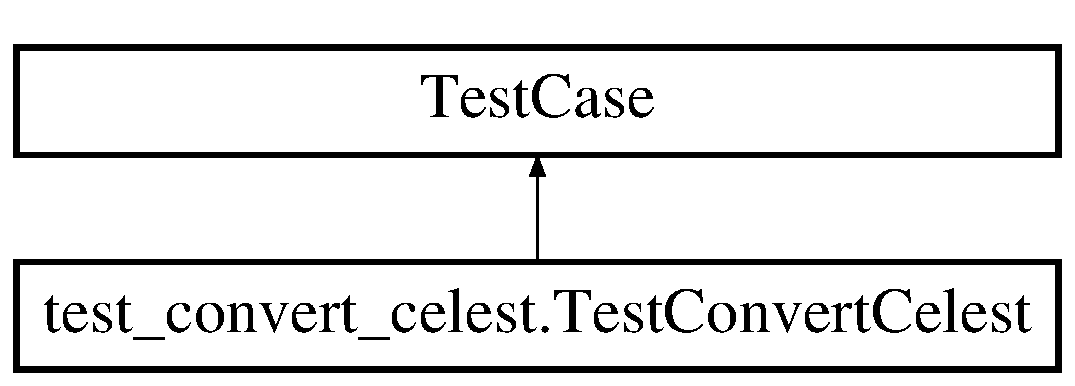
\includegraphics[height=2.000000cm]{classtest__convert__celest_1_1_test_convert_celest}
\end{center}
\end{figure}
\subsection*{Public Member Functions}
\begin{DoxyCompactItemize}
\item 
def \hyperlink{classtest__convert__celest_1_1_test_convert_celest_a8fd1939ab7d996c7923408df42a13b0f}{set\-Up}
\item 
def \hyperlink{classtest__convert__celest_1_1_test_convert_celest_aaf41fa49cf37ddbad86b6e6af4827db1}{tear\-Down}
\item 
def \hyperlink{classtest__convert__celest_1_1_test_convert_celest_a086e6c724cb8acc6d7bfbca28db421b7}{test\-\_\-poles}
\item 
def \hyperlink{classtest__convert__celest_1_1_test_convert_celest_a5fb62371cbd71130b2f2b55792e7595e}{test\-\_\-quadrants}
\end{DoxyCompactItemize}


\subsection{Member Function Documentation}
\hypertarget{classtest__convert__celest_1_1_test_convert_celest_a8fd1939ab7d996c7923408df42a13b0f}{\index{test\-\_\-convert\-\_\-celest\-::\-Test\-Convert\-Celest@{test\-\_\-convert\-\_\-celest\-::\-Test\-Convert\-Celest}!set\-Up@{set\-Up}}
\index{set\-Up@{set\-Up}!test_convert_celest::TestConvertCelest@{test\-\_\-convert\-\_\-celest\-::\-Test\-Convert\-Celest}}
\subsubsection[{set\-Up}]{\setlength{\rightskip}{0pt plus 5cm}def test\-\_\-convert\-\_\-celest.\-Test\-Convert\-Celest.\-set\-Up (
\begin{DoxyParamCaption}
\item[{}]{self}
\end{DoxyParamCaption}
)}}\label{classtest__convert__celest_1_1_test_convert_celest_a8fd1939ab7d996c7923408df42a13b0f}
\hypertarget{classtest__convert__celest_1_1_test_convert_celest_aaf41fa49cf37ddbad86b6e6af4827db1}{\index{test\-\_\-convert\-\_\-celest\-::\-Test\-Convert\-Celest@{test\-\_\-convert\-\_\-celest\-::\-Test\-Convert\-Celest}!tear\-Down@{tear\-Down}}
\index{tear\-Down@{tear\-Down}!test_convert_celest::TestConvertCelest@{test\-\_\-convert\-\_\-celest\-::\-Test\-Convert\-Celest}}
\subsubsection[{tear\-Down}]{\setlength{\rightskip}{0pt plus 5cm}def test\-\_\-convert\-\_\-celest.\-Test\-Convert\-Celest.\-tear\-Down (
\begin{DoxyParamCaption}
\item[{}]{self}
\end{DoxyParamCaption}
)}}\label{classtest__convert__celest_1_1_test_convert_celest_aaf41fa49cf37ddbad86b6e6af4827db1}
\hypertarget{classtest__convert__celest_1_1_test_convert_celest_a086e6c724cb8acc6d7bfbca28db421b7}{\index{test\-\_\-convert\-\_\-celest\-::\-Test\-Convert\-Celest@{test\-\_\-convert\-\_\-celest\-::\-Test\-Convert\-Celest}!test\-\_\-poles@{test\-\_\-poles}}
\index{test\-\_\-poles@{test\-\_\-poles}!test_convert_celest::TestConvertCelest@{test\-\_\-convert\-\_\-celest\-::\-Test\-Convert\-Celest}}
\subsubsection[{test\-\_\-poles}]{\setlength{\rightskip}{0pt plus 5cm}def test\-\_\-convert\-\_\-celest.\-Test\-Convert\-Celest.\-test\-\_\-poles (
\begin{DoxyParamCaption}
\item[{}]{self}
\end{DoxyParamCaption}
)}}\label{classtest__convert__celest_1_1_test_convert_celest_a086e6c724cb8acc6d7bfbca28db421b7}
\hypertarget{classtest__convert__celest_1_1_test_convert_celest_a5fb62371cbd71130b2f2b55792e7595e}{\index{test\-\_\-convert\-\_\-celest\-::\-Test\-Convert\-Celest@{test\-\_\-convert\-\_\-celest\-::\-Test\-Convert\-Celest}!test\-\_\-quadrants@{test\-\_\-quadrants}}
\index{test\-\_\-quadrants@{test\-\_\-quadrants}!test_convert_celest::TestConvertCelest@{test\-\_\-convert\-\_\-celest\-::\-Test\-Convert\-Celest}}
\subsubsection[{test\-\_\-quadrants}]{\setlength{\rightskip}{0pt plus 5cm}def test\-\_\-convert\-\_\-celest.\-Test\-Convert\-Celest.\-test\-\_\-quadrants (
\begin{DoxyParamCaption}
\item[{}]{self}
\end{DoxyParamCaption}
)}}\label{classtest__convert__celest_1_1_test_convert_celest_a5fb62371cbd71130b2f2b55792e7595e}


The documentation for this class was generated from the following file\-:\begin{DoxyCompactItemize}
\item 
amonpy/tools/test/\hyperlink{test__convert__celest_8py}{test\-\_\-convert\-\_\-celest.\-py}\end{DoxyCompactItemize}

\hypertarget{classtest__dbaccess_1_1_test_d_baccess}{\section{test\-\_\-dbaccess.\-Test\-D\-Baccess Class Reference}
\label{classtest__dbaccess_1_1_test_d_baccess}\index{test\-\_\-dbaccess.\-Test\-D\-Baccess@{test\-\_\-dbaccess.\-Test\-D\-Baccess}}
}
Inheritance diagram for test\-\_\-dbaccess.\-Test\-D\-Baccess\-:\begin{figure}[H]
\begin{center}
\leavevmode
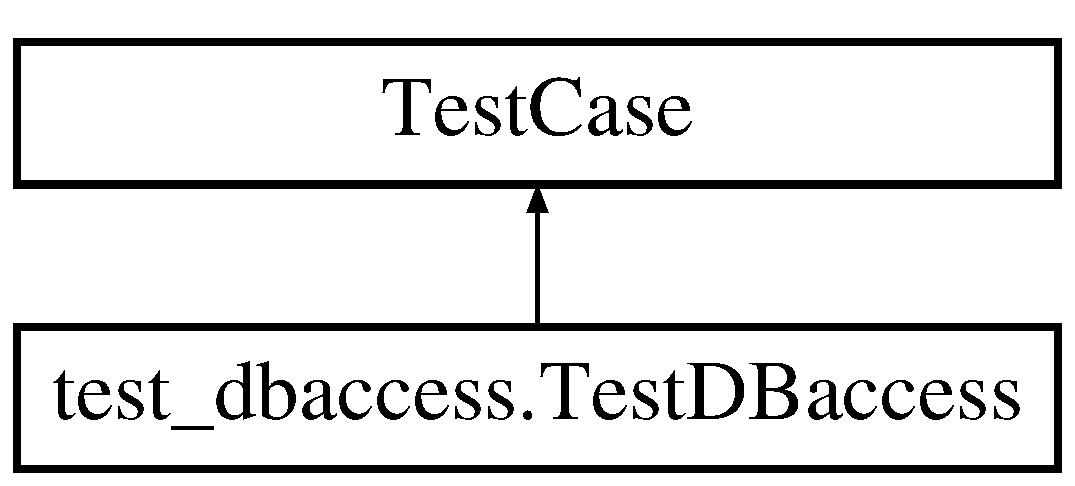
\includegraphics[height=2.000000cm]{dd/dd1/classtest__dbaccess_1_1_test_d_baccess}
\end{center}
\end{figure}
\subsection*{Public Member Functions}
\begin{DoxyCompactItemize}
\item 
def \hyperlink{classtest__dbaccess_1_1_test_d_baccess_a772a12714e7eabb3e425a38199f615d8}{set\-Up}
\item 
def \hyperlink{classtest__dbaccess_1_1_test_d_baccess_a56792c35c47f03be12bc1880b7180adc}{tear\-Down}
\item 
def \hyperlink{classtest__dbaccess_1_1_test_d_baccess_a0eec2c586e1243ab3d9f24f208446494}{test1\-\_\-readfile}
\end{DoxyCompactItemize}


\subsection{Detailed Description}


Definition at line 12 of file test\-\_\-dbaccess.\-py.



\subsection{Member Function Documentation}
\hypertarget{classtest__dbaccess_1_1_test_d_baccess_a772a12714e7eabb3e425a38199f615d8}{\index{test\-\_\-dbaccess\-::\-Test\-D\-Baccess@{test\-\_\-dbaccess\-::\-Test\-D\-Baccess}!set\-Up@{set\-Up}}
\index{set\-Up@{set\-Up}!test_dbaccess::TestDBaccess@{test\-\_\-dbaccess\-::\-Test\-D\-Baccess}}
\subsubsection[{set\-Up}]{\setlength{\rightskip}{0pt plus 5cm}def test\-\_\-dbaccess.\-Test\-D\-Baccess.\-set\-Up (
\begin{DoxyParamCaption}
\item[{}]{self}
\end{DoxyParamCaption}
)}}\label{classtest__dbaccess_1_1_test_d_baccess_a772a12714e7eabb3e425a38199f615d8}


Definition at line 13 of file test\-\_\-dbaccess.\-py.

\hypertarget{classtest__dbaccess_1_1_test_d_baccess_a56792c35c47f03be12bc1880b7180adc}{\index{test\-\_\-dbaccess\-::\-Test\-D\-Baccess@{test\-\_\-dbaccess\-::\-Test\-D\-Baccess}!tear\-Down@{tear\-Down}}
\index{tear\-Down@{tear\-Down}!test_dbaccess::TestDBaccess@{test\-\_\-dbaccess\-::\-Test\-D\-Baccess}}
\subsubsection[{tear\-Down}]{\setlength{\rightskip}{0pt plus 5cm}def test\-\_\-dbaccess.\-Test\-D\-Baccess.\-tear\-Down (
\begin{DoxyParamCaption}
\item[{}]{self}
\end{DoxyParamCaption}
)}}\label{classtest__dbaccess_1_1_test_d_baccess_a56792c35c47f03be12bc1880b7180adc}


Definition at line 18 of file test\-\_\-dbaccess.\-py.

\hypertarget{classtest__dbaccess_1_1_test_d_baccess_a0eec2c586e1243ab3d9f24f208446494}{\index{test\-\_\-dbaccess\-::\-Test\-D\-Baccess@{test\-\_\-dbaccess\-::\-Test\-D\-Baccess}!test1\-\_\-readfile@{test1\-\_\-readfile}}
\index{test1\-\_\-readfile@{test1\-\_\-readfile}!test_dbaccess::TestDBaccess@{test\-\_\-dbaccess\-::\-Test\-D\-Baccess}}
\subsubsection[{test1\-\_\-readfile}]{\setlength{\rightskip}{0pt plus 5cm}def test\-\_\-dbaccess.\-Test\-D\-Baccess.\-test1\-\_\-readfile (
\begin{DoxyParamCaption}
\item[{}]{self}
\end{DoxyParamCaption}
)}}\label{classtest__dbaccess_1_1_test_d_baccess_a0eec2c586e1243ab3d9f24f208446494}


Definition at line 23 of file test\-\_\-dbaccess.\-py.



The documentation for this class was generated from the following file\-:\begin{DoxyCompactItemize}
\item 
amonpy/ops/test/\hyperlink{test__dbaccess_8py}{test\-\_\-dbaccess.\-py}\end{DoxyCompactItemize}

\hypertarget{classamonpy_1_1dbase_1_1test_1_1test__db__class_1_1_test_d_bclass}{\section{amonpy.\-dbase.\-test.\-test\-\_\-db\-\_\-class.\-Test\-D\-Bclass Class Reference}
\label{classamonpy_1_1dbase_1_1test_1_1test__db__class_1_1_test_d_bclass}\index{amonpy.\-dbase.\-test.\-test\-\_\-db\-\_\-class.\-Test\-D\-Bclass@{amonpy.\-dbase.\-test.\-test\-\_\-db\-\_\-class.\-Test\-D\-Bclass}}
}


Unit tests for db\-\_\-class module.  


Inheritance diagram for amonpy.\-dbase.\-test.\-test\-\_\-db\-\_\-class.\-Test\-D\-Bclass\-:\begin{figure}[H]
\begin{center}
\leavevmode
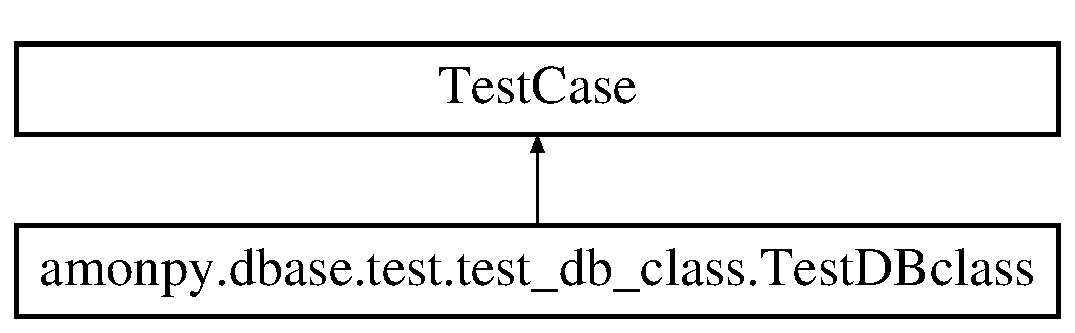
\includegraphics[height=2.000000cm]{df/d26/classamonpy_1_1dbase_1_1test_1_1test__db__class_1_1_test_d_bclass}
\end{center}
\end{figure}
\subsection*{Public Member Functions}
\begin{DoxyCompactItemize}
\item 
def \hyperlink{classamonpy_1_1dbase_1_1test_1_1test__db__class_1_1_test_d_bclass_a31494b390c6fc80f95278686176ec5f8}{set\-Up}
\item 
def \hyperlink{classamonpy_1_1dbase_1_1test_1_1test__db__class_1_1_test_d_bclass_a88a8aa65c07160914a02c08b7a640ba5}{tear\-Down}
\item 
def \hyperlink{classamonpy_1_1dbase_1_1test_1_1test__db__class_1_1_test_d_bclass_a97be3dd99ebc1f8b14693db6915777d1}{test1\-\_\-init\-\_\-del}
\item 
def \hyperlink{classamonpy_1_1dbase_1_1test_1_1test__db__class_1_1_test_d_bclass_a6ef3d28a9cd7eed053496e50343dc739}{test3\-\_\-forprint}
\item 
def \hyperlink{classamonpy_1_1dbase_1_1test_1_1test__db__class_1_1_test_d_bclass_a6617ea3ec878545db8b3c18266b4f7b3}{test5\-\_\-list}
\item 
def \hyperlink{classamonpy_1_1dbase_1_1test_1_1test__db__class_1_1_test_d_bclass_a7f16f16b2c55311ba8574e012c28932b}{test6\-\_\-\-Event\-Stream\-Config}
\item 
def \hyperlink{classamonpy_1_1dbase_1_1test_1_1test__db__class_1_1_test_d_bclass_af08a45abf4c3d741fe633431598387e5}{test7\-\_\-del\-\_\-\-Alert}
\item 
def \hyperlink{classamonpy_1_1dbase_1_1test_1_1test__db__class_1_1_test_d_bclass_a6dbca107c4d681938a6d63b4f917d849}{test8\-\_\-print\-\_\-\-Alert}
\item 
def \hyperlink{classamonpy_1_1dbase_1_1test_1_1test__db__class_1_1_test_d_bclass_a314fdaa0e19025b59e6409e85f96ab6a}{test9\-\_\-\-Alert\-Config}
\end{DoxyCompactItemize}


\subsection{Detailed Description}
Unit tests for db\-\_\-class module. 

Definition at line 17 of file test\-\_\-db\-\_\-class.\-py.



\subsection{Member Function Documentation}
\hypertarget{classamonpy_1_1dbase_1_1test_1_1test__db__class_1_1_test_d_bclass_a31494b390c6fc80f95278686176ec5f8}{\index{amonpy\-::dbase\-::test\-::test\-\_\-db\-\_\-class\-::\-Test\-D\-Bclass@{amonpy\-::dbase\-::test\-::test\-\_\-db\-\_\-class\-::\-Test\-D\-Bclass}!set\-Up@{set\-Up}}
\index{set\-Up@{set\-Up}!amonpy::dbase::test::test_db_class::TestDBclass@{amonpy\-::dbase\-::test\-::test\-\_\-db\-\_\-class\-::\-Test\-D\-Bclass}}
\subsubsection[{set\-Up}]{\setlength{\rightskip}{0pt plus 5cm}def amonpy.\-dbase.\-test.\-test\-\_\-db\-\_\-class.\-Test\-D\-Bclass.\-set\-Up (
\begin{DoxyParamCaption}
\item[{}]{self}
\end{DoxyParamCaption}
)}}\label{classamonpy_1_1dbase_1_1test_1_1test__db__class_1_1_test_d_bclass_a31494b390c6fc80f95278686176ec5f8}


Definition at line 18 of file test\-\_\-db\-\_\-class.\-py.

\hypertarget{classamonpy_1_1dbase_1_1test_1_1test__db__class_1_1_test_d_bclass_a88a8aa65c07160914a02c08b7a640ba5}{\index{amonpy\-::dbase\-::test\-::test\-\_\-db\-\_\-class\-::\-Test\-D\-Bclass@{amonpy\-::dbase\-::test\-::test\-\_\-db\-\_\-class\-::\-Test\-D\-Bclass}!tear\-Down@{tear\-Down}}
\index{tear\-Down@{tear\-Down}!amonpy::dbase::test::test_db_class::TestDBclass@{amonpy\-::dbase\-::test\-::test\-\_\-db\-\_\-class\-::\-Test\-D\-Bclass}}
\subsubsection[{tear\-Down}]{\setlength{\rightskip}{0pt plus 5cm}def amonpy.\-dbase.\-test.\-test\-\_\-db\-\_\-class.\-Test\-D\-Bclass.\-tear\-Down (
\begin{DoxyParamCaption}
\item[{}]{self}
\end{DoxyParamCaption}
)}}\label{classamonpy_1_1dbase_1_1test_1_1test__db__class_1_1_test_d_bclass_a88a8aa65c07160914a02c08b7a640ba5}


Definition at line 30 of file test\-\_\-db\-\_\-class.\-py.

\hypertarget{classamonpy_1_1dbase_1_1test_1_1test__db__class_1_1_test_d_bclass_a97be3dd99ebc1f8b14693db6915777d1}{\index{amonpy\-::dbase\-::test\-::test\-\_\-db\-\_\-class\-::\-Test\-D\-Bclass@{amonpy\-::dbase\-::test\-::test\-\_\-db\-\_\-class\-::\-Test\-D\-Bclass}!test1\-\_\-init\-\_\-del@{test1\-\_\-init\-\_\-del}}
\index{test1\-\_\-init\-\_\-del@{test1\-\_\-init\-\_\-del}!amonpy::dbase::test::test_db_class::TestDBclass@{amonpy\-::dbase\-::test\-::test\-\_\-db\-\_\-class\-::\-Test\-D\-Bclass}}
\subsubsection[{test1\-\_\-init\-\_\-del}]{\setlength{\rightskip}{0pt plus 5cm}def amonpy.\-dbase.\-test.\-test\-\_\-db\-\_\-class.\-Test\-D\-Bclass.\-test1\-\_\-init\-\_\-del (
\begin{DoxyParamCaption}
\item[{}]{self}
\end{DoxyParamCaption}
)}}\label{classamonpy_1_1dbase_1_1test_1_1test__db__class_1_1_test_d_bclass_a97be3dd99ebc1f8b14693db6915777d1}


Definition at line 35 of file test\-\_\-db\-\_\-class.\-py.

\hypertarget{classamonpy_1_1dbase_1_1test_1_1test__db__class_1_1_test_d_bclass_a6ef3d28a9cd7eed053496e50343dc739}{\index{amonpy\-::dbase\-::test\-::test\-\_\-db\-\_\-class\-::\-Test\-D\-Bclass@{amonpy\-::dbase\-::test\-::test\-\_\-db\-\_\-class\-::\-Test\-D\-Bclass}!test3\-\_\-forprint@{test3\-\_\-forprint}}
\index{test3\-\_\-forprint@{test3\-\_\-forprint}!amonpy::dbase::test::test_db_class::TestDBclass@{amonpy\-::dbase\-::test\-::test\-\_\-db\-\_\-class\-::\-Test\-D\-Bclass}}
\subsubsection[{test3\-\_\-forprint}]{\setlength{\rightskip}{0pt plus 5cm}def amonpy.\-dbase.\-test.\-test\-\_\-db\-\_\-class.\-Test\-D\-Bclass.\-test3\-\_\-forprint (
\begin{DoxyParamCaption}
\item[{}]{self}
\end{DoxyParamCaption}
)}}\label{classamonpy_1_1dbase_1_1test_1_1test__db__class_1_1_test_d_bclass_a6ef3d28a9cd7eed053496e50343dc739}


Definition at line 53 of file test\-\_\-db\-\_\-class.\-py.

\hypertarget{classamonpy_1_1dbase_1_1test_1_1test__db__class_1_1_test_d_bclass_a6617ea3ec878545db8b3c18266b4f7b3}{\index{amonpy\-::dbase\-::test\-::test\-\_\-db\-\_\-class\-::\-Test\-D\-Bclass@{amonpy\-::dbase\-::test\-::test\-\_\-db\-\_\-class\-::\-Test\-D\-Bclass}!test5\-\_\-list@{test5\-\_\-list}}
\index{test5\-\_\-list@{test5\-\_\-list}!amonpy::dbase::test::test_db_class::TestDBclass@{amonpy\-::dbase\-::test\-::test\-\_\-db\-\_\-class\-::\-Test\-D\-Bclass}}
\subsubsection[{test5\-\_\-list}]{\setlength{\rightskip}{0pt plus 5cm}def amonpy.\-dbase.\-test.\-test\-\_\-db\-\_\-class.\-Test\-D\-Bclass.\-test5\-\_\-list (
\begin{DoxyParamCaption}
\item[{}]{self}
\end{DoxyParamCaption}
)}}\label{classamonpy_1_1dbase_1_1test_1_1test__db__class_1_1_test_d_bclass_a6617ea3ec878545db8b3c18266b4f7b3}


Definition at line 71 of file test\-\_\-db\-\_\-class.\-py.

\hypertarget{classamonpy_1_1dbase_1_1test_1_1test__db__class_1_1_test_d_bclass_a7f16f16b2c55311ba8574e012c28932b}{\index{amonpy\-::dbase\-::test\-::test\-\_\-db\-\_\-class\-::\-Test\-D\-Bclass@{amonpy\-::dbase\-::test\-::test\-\_\-db\-\_\-class\-::\-Test\-D\-Bclass}!test6\-\_\-\-Event\-Stream\-Config@{test6\-\_\-\-Event\-Stream\-Config}}
\index{test6\-\_\-\-Event\-Stream\-Config@{test6\-\_\-\-Event\-Stream\-Config}!amonpy::dbase::test::test_db_class::TestDBclass@{amonpy\-::dbase\-::test\-::test\-\_\-db\-\_\-class\-::\-Test\-D\-Bclass}}
\subsubsection[{test6\-\_\-\-Event\-Stream\-Config}]{\setlength{\rightskip}{0pt plus 5cm}def amonpy.\-dbase.\-test.\-test\-\_\-db\-\_\-class.\-Test\-D\-Bclass.\-test6\-\_\-\-Event\-Stream\-Config (
\begin{DoxyParamCaption}
\item[{}]{self}
\end{DoxyParamCaption}
)}}\label{classamonpy_1_1dbase_1_1test_1_1test__db__class_1_1_test_d_bclass_a7f16f16b2c55311ba8574e012c28932b}


Definition at line 78 of file test\-\_\-db\-\_\-class.\-py.

\hypertarget{classamonpy_1_1dbase_1_1test_1_1test__db__class_1_1_test_d_bclass_af08a45abf4c3d741fe633431598387e5}{\index{amonpy\-::dbase\-::test\-::test\-\_\-db\-\_\-class\-::\-Test\-D\-Bclass@{amonpy\-::dbase\-::test\-::test\-\_\-db\-\_\-class\-::\-Test\-D\-Bclass}!test7\-\_\-del\-\_\-\-Alert@{test7\-\_\-del\-\_\-\-Alert}}
\index{test7\-\_\-del\-\_\-\-Alert@{test7\-\_\-del\-\_\-\-Alert}!amonpy::dbase::test::test_db_class::TestDBclass@{amonpy\-::dbase\-::test\-::test\-\_\-db\-\_\-class\-::\-Test\-D\-Bclass}}
\subsubsection[{test7\-\_\-del\-\_\-\-Alert}]{\setlength{\rightskip}{0pt plus 5cm}def amonpy.\-dbase.\-test.\-test\-\_\-db\-\_\-class.\-Test\-D\-Bclass.\-test7\-\_\-del\-\_\-\-Alert (
\begin{DoxyParamCaption}
\item[{}]{self}
\end{DoxyParamCaption}
)}}\label{classamonpy_1_1dbase_1_1test_1_1test__db__class_1_1_test_d_bclass_af08a45abf4c3d741fe633431598387e5}


Definition at line 91 of file test\-\_\-db\-\_\-class.\-py.

\hypertarget{classamonpy_1_1dbase_1_1test_1_1test__db__class_1_1_test_d_bclass_a6dbca107c4d681938a6d63b4f917d849}{\index{amonpy\-::dbase\-::test\-::test\-\_\-db\-\_\-class\-::\-Test\-D\-Bclass@{amonpy\-::dbase\-::test\-::test\-\_\-db\-\_\-class\-::\-Test\-D\-Bclass}!test8\-\_\-print\-\_\-\-Alert@{test8\-\_\-print\-\_\-\-Alert}}
\index{test8\-\_\-print\-\_\-\-Alert@{test8\-\_\-print\-\_\-\-Alert}!amonpy::dbase::test::test_db_class::TestDBclass@{amonpy\-::dbase\-::test\-::test\-\_\-db\-\_\-class\-::\-Test\-D\-Bclass}}
\subsubsection[{test8\-\_\-print\-\_\-\-Alert}]{\setlength{\rightskip}{0pt plus 5cm}def amonpy.\-dbase.\-test.\-test\-\_\-db\-\_\-class.\-Test\-D\-Bclass.\-test8\-\_\-print\-\_\-\-Alert (
\begin{DoxyParamCaption}
\item[{}]{self}
\end{DoxyParamCaption}
)}}\label{classamonpy_1_1dbase_1_1test_1_1test__db__class_1_1_test_d_bclass_a6dbca107c4d681938a6d63b4f917d849}


Definition at line 100 of file test\-\_\-db\-\_\-class.\-py.

\hypertarget{classamonpy_1_1dbase_1_1test_1_1test__db__class_1_1_test_d_bclass_a314fdaa0e19025b59e6409e85f96ab6a}{\index{amonpy\-::dbase\-::test\-::test\-\_\-db\-\_\-class\-::\-Test\-D\-Bclass@{amonpy\-::dbase\-::test\-::test\-\_\-db\-\_\-class\-::\-Test\-D\-Bclass}!test9\-\_\-\-Alert\-Config@{test9\-\_\-\-Alert\-Config}}
\index{test9\-\_\-\-Alert\-Config@{test9\-\_\-\-Alert\-Config}!amonpy::dbase::test::test_db_class::TestDBclass@{amonpy\-::dbase\-::test\-::test\-\_\-db\-\_\-class\-::\-Test\-D\-Bclass}}
\subsubsection[{test9\-\_\-\-Alert\-Config}]{\setlength{\rightskip}{0pt plus 5cm}def amonpy.\-dbase.\-test.\-test\-\_\-db\-\_\-class.\-Test\-D\-Bclass.\-test9\-\_\-\-Alert\-Config (
\begin{DoxyParamCaption}
\item[{}]{self}
\end{DoxyParamCaption}
)}}\label{classamonpy_1_1dbase_1_1test_1_1test__db__class_1_1_test_d_bclass_a314fdaa0e19025b59e6409e85f96ab6a}


Definition at line 108 of file test\-\_\-db\-\_\-class.\-py.



The documentation for this class was generated from the following file\-:\begin{DoxyCompactItemize}
\item 
amonpy/dbase/test/\hyperlink{test__db__class_8py}{test\-\_\-db\-\_\-class.\-py}\end{DoxyCompactItemize}

\hypertarget{classamonpy_1_1dbase_1_1test_1_1test__db__read_1_1_test_d_b_read}{\section{amonpy.\-dbase.\-test.\-test\-\_\-db\-\_\-read.\-Test\-D\-B\-Read Class Reference}
\label{classamonpy_1_1dbase_1_1test_1_1test__db__read_1_1_test_d_b_read}\index{amonpy.\-dbase.\-test.\-test\-\_\-db\-\_\-read.\-Test\-D\-B\-Read@{amonpy.\-dbase.\-test.\-test\-\_\-db\-\_\-read.\-Test\-D\-B\-Read}}
}
Inheritance diagram for amonpy.\-dbase.\-test.\-test\-\_\-db\-\_\-read.\-Test\-D\-B\-Read\-:\begin{figure}[H]
\begin{center}
\leavevmode
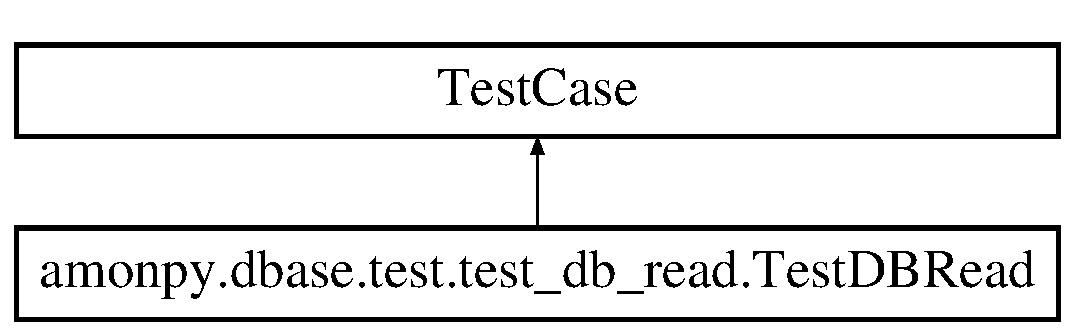
\includegraphics[height=2.000000cm]{classamonpy_1_1dbase_1_1test_1_1test__db__read_1_1_test_d_b_read}
\end{center}
\end{figure}
\subsection*{Public Member Functions}
\begin{DoxyCompactItemize}
\item 
def \hyperlink{classamonpy_1_1dbase_1_1test_1_1test__db__read_1_1_test_d_b_read_a3d42ef1ed1ec53504c475d0db682fc1e}{set\-Up}
\item 
def \hyperlink{classamonpy_1_1dbase_1_1test_1_1test__db__read_1_1_test_d_b_read_a5e6de8d1c39f5c64ac66b5329d7803ba}{tear\-Down}
\item 
def \hyperlink{classamonpy_1_1dbase_1_1test_1_1test__db__read_1_1_test_d_b_read_a8eef1ba4193c4b630467e5cc4356e326}{test\-Read\-Single}
\item 
def \hyperlink{classamonpy_1_1dbase_1_1test_1_1test__db__read_1_1_test_d_b_read_af5b8a121cd312c79b9a96f14225895cd}{test\-Read\-Time\-Slice}
\item 
def \hyperlink{classamonpy_1_1dbase_1_1test_1_1test__db__read_1_1_test_d_b_read_ad58e247d7332ccd18c21296b68ef3944}{test\-Read\-Event\-Config}
\item 
def \hyperlink{classamonpy_1_1dbase_1_1test_1_1test__db__read_1_1_test_d_b_read_a88bf26659e5ad77f96e49347e527ea1c}{test\-Read\-Alert\-Config}
\item 
def \hyperlink{classamonpy_1_1dbase_1_1test_1_1test__db__read_1_1_test_d_b_read_a9e83f573f0f9825c75e585d2e6707283}{test\-Read\-Alert}
\item 
def \hyperlink{classamonpy_1_1dbase_1_1test_1_1test__db__read_1_1_test_d_b_read_a521e28d6ad16e03b0a6ad6cbfe06f725}{test\-Read\-Alert\-Time\-Slice}
\item 
def \hyperlink{classamonpy_1_1dbase_1_1test_1_1test__db__read_1_1_test_d_b_read_a21c5b2538f4d5adee20f64bc377d7905}{test\-Read\-Parameter\-Single}
\end{DoxyCompactItemize}
\subsection*{Public Attributes}
\begin{DoxyCompactItemize}
\item 
\hyperlink{classamonpy_1_1dbase_1_1test_1_1test__db__read_1_1_test_d_b_read_a6700613b2e7f2b5a5f84f8fa3b8e8e3f}{real\-Archive}
\item 
\hyperlink{classamonpy_1_1dbase_1_1test_1_1test__db__read_1_1_test_d_b_read_aef02f233501a4c3d5f1b005a1c0c0d72}{Host\-Fancy\-Name}
\item 
\hyperlink{classamonpy_1_1dbase_1_1test_1_1test__db__read_1_1_test_d_b_read_a9ed55e19e8187469a496695884509101}{User\-Fancy\-Name}
\item 
\hyperlink{classamonpy_1_1dbase_1_1test_1_1test__db__read_1_1_test_d_b_read_af3fe3e1b6f4d40624da8b3168058e355}{Password\-Fancy}
\item 
\hyperlink{classamonpy_1_1dbase_1_1test_1_1test__db__read_1_1_test_d_b_read_af7baa96afc495b6ddf3b2a9c053e6273}{D\-B\-Fancy\-Name}
\item 
\hyperlink{classamonpy_1_1dbase_1_1test_1_1test__db__read_1_1_test_d_b_read_a4ec0f5238616b6faf18b5754b8f708d4}{D\-B\-Fancy\-Name2}
\item 
\hyperlink{classamonpy_1_1dbase_1_1test_1_1test__db__read_1_1_test_d_b_read_ac7f82aeb05869690ebcd4c7619117943}{Stream\-Fancy\-Name}
\item 
\hyperlink{classamonpy_1_1dbase_1_1test_1_1test__db__read_1_1_test_d_b_read_aab94ea32aa54e6d2cca5f68e1387be51}{Event\-I\-D}
\item 
\hyperlink{classamonpy_1_1dbase_1_1test_1_1test__db__read_1_1_test_d_b_read_a6f44b33da586a4e0dfba810ab1692852}{Event\-Rev}
\item 
\hyperlink{classamonpy_1_1dbase_1_1test_1_1test__db__read_1_1_test_d_b_read_aec46e79a01fcb17284df6e0ccf8af8fc}{Time\-Start}
\item 
\hyperlink{classamonpy_1_1dbase_1_1test_1_1test__db__read_1_1_test_d_b_read_aa69e0701a1ef6f93dc6053a6cad634dd}{Time\-Slice}
\item 
\hyperlink{classamonpy_1_1dbase_1_1test_1_1test__db__read_1_1_test_d_b_read_a3ee527a724daeb372b8fe60472ba5ce4}{Time\-Stop}
\item 
\hyperlink{classamonpy_1_1dbase_1_1test_1_1test__db__read_1_1_test_d_b_read_a762f69bcd3574f95324c3874f7712b6b}{Alert\-Stream}
\item 
\hyperlink{classamonpy_1_1dbase_1_1test_1_1test__db__read_1_1_test_d_b_read_ab8058162f86c23241a86b9c23671aa26}{Alert\-Rev}
\item 
\hyperlink{classamonpy_1_1dbase_1_1test_1_1test__db__read_1_1_test_d_b_read_adc41ecfc3c76fdd34341069786072911}{Alert\-I\-D}
\item 
\hyperlink{classamonpy_1_1dbase_1_1test_1_1test__db__read_1_1_test_d_b_read_a56e876914366660147a59978cc999d79}{Parameter\-Name}
\item 
\hyperlink{classamonpy_1_1dbase_1_1test_1_1test__db__read_1_1_test_d_b_read_ad24d241f9e0ae66844f79480d2ddfc93}{Stream\-Fancy\-Name2}
\item 
\hyperlink{classamonpy_1_1dbase_1_1test_1_1test__db__read_1_1_test_d_b_read_a16a0f37d14afbd09c98a8b403f177693}{Event\-I\-D2}
\item 
\hyperlink{classamonpy_1_1dbase_1_1test_1_1test__db__read_1_1_test_d_b_read_a857e1e2e776352c3615410f13f8e7f7b}{Event\-Rev2}
\item 
\hyperlink{classamonpy_1_1dbase_1_1test_1_1test__db__read_1_1_test_d_b_read_ae601f95c55daa72d31a753475e4aa7f5}{Time\-Start2}
\end{DoxyCompactItemize}


\subsection{Detailed Description}
\begin{DoxyVerb}   Unit tests for db_read module.
\end{DoxyVerb}
 

\subsection{Member Function Documentation}
\hypertarget{classamonpy_1_1dbase_1_1test_1_1test__db__read_1_1_test_d_b_read_a3d42ef1ed1ec53504c475d0db682fc1e}{\index{amonpy\-::dbase\-::test\-::test\-\_\-db\-\_\-read\-::\-Test\-D\-B\-Read@{amonpy\-::dbase\-::test\-::test\-\_\-db\-\_\-read\-::\-Test\-D\-B\-Read}!set\-Up@{set\-Up}}
\index{set\-Up@{set\-Up}!amonpy::dbase::test::test_db_read::TestDBRead@{amonpy\-::dbase\-::test\-::test\-\_\-db\-\_\-read\-::\-Test\-D\-B\-Read}}
\subsubsection[{set\-Up}]{\setlength{\rightskip}{0pt plus 5cm}def amonpy.\-dbase.\-test.\-test\-\_\-db\-\_\-read.\-Test\-D\-B\-Read.\-set\-Up (
\begin{DoxyParamCaption}
\item[{}]{self}
\end{DoxyParamCaption}
)}}\label{classamonpy_1_1dbase_1_1test_1_1test__db__read_1_1_test_d_b_read_a3d42ef1ed1ec53504c475d0db682fc1e}
\hypertarget{classamonpy_1_1dbase_1_1test_1_1test__db__read_1_1_test_d_b_read_a5e6de8d1c39f5c64ac66b5329d7803ba}{\index{amonpy\-::dbase\-::test\-::test\-\_\-db\-\_\-read\-::\-Test\-D\-B\-Read@{amonpy\-::dbase\-::test\-::test\-\_\-db\-\_\-read\-::\-Test\-D\-B\-Read}!tear\-Down@{tear\-Down}}
\index{tear\-Down@{tear\-Down}!amonpy::dbase::test::test_db_read::TestDBRead@{amonpy\-::dbase\-::test\-::test\-\_\-db\-\_\-read\-::\-Test\-D\-B\-Read}}
\subsubsection[{tear\-Down}]{\setlength{\rightskip}{0pt plus 5cm}def amonpy.\-dbase.\-test.\-test\-\_\-db\-\_\-read.\-Test\-D\-B\-Read.\-tear\-Down (
\begin{DoxyParamCaption}
\item[{}]{self}
\end{DoxyParamCaption}
)}}\label{classamonpy_1_1dbase_1_1test_1_1test__db__read_1_1_test_d_b_read_a5e6de8d1c39f5c64ac66b5329d7803ba}
\hypertarget{classamonpy_1_1dbase_1_1test_1_1test__db__read_1_1_test_d_b_read_a9e83f573f0f9825c75e585d2e6707283}{\index{amonpy\-::dbase\-::test\-::test\-\_\-db\-\_\-read\-::\-Test\-D\-B\-Read@{amonpy\-::dbase\-::test\-::test\-\_\-db\-\_\-read\-::\-Test\-D\-B\-Read}!test\-Read\-Alert@{test\-Read\-Alert}}
\index{test\-Read\-Alert@{test\-Read\-Alert}!amonpy::dbase::test::test_db_read::TestDBRead@{amonpy\-::dbase\-::test\-::test\-\_\-db\-\_\-read\-::\-Test\-D\-B\-Read}}
\subsubsection[{test\-Read\-Alert}]{\setlength{\rightskip}{0pt plus 5cm}def amonpy.\-dbase.\-test.\-test\-\_\-db\-\_\-read.\-Test\-D\-B\-Read.\-test\-Read\-Alert (
\begin{DoxyParamCaption}
\item[{}]{self}
\end{DoxyParamCaption}
)}}\label{classamonpy_1_1dbase_1_1test_1_1test__db__read_1_1_test_d_b_read_a9e83f573f0f9825c75e585d2e6707283}
\hypertarget{classamonpy_1_1dbase_1_1test_1_1test__db__read_1_1_test_d_b_read_a88bf26659e5ad77f96e49347e527ea1c}{\index{amonpy\-::dbase\-::test\-::test\-\_\-db\-\_\-read\-::\-Test\-D\-B\-Read@{amonpy\-::dbase\-::test\-::test\-\_\-db\-\_\-read\-::\-Test\-D\-B\-Read}!test\-Read\-Alert\-Config@{test\-Read\-Alert\-Config}}
\index{test\-Read\-Alert\-Config@{test\-Read\-Alert\-Config}!amonpy::dbase::test::test_db_read::TestDBRead@{amonpy\-::dbase\-::test\-::test\-\_\-db\-\_\-read\-::\-Test\-D\-B\-Read}}
\subsubsection[{test\-Read\-Alert\-Config}]{\setlength{\rightskip}{0pt plus 5cm}def amonpy.\-dbase.\-test.\-test\-\_\-db\-\_\-read.\-Test\-D\-B\-Read.\-test\-Read\-Alert\-Config (
\begin{DoxyParamCaption}
\item[{}]{self}
\end{DoxyParamCaption}
)}}\label{classamonpy_1_1dbase_1_1test_1_1test__db__read_1_1_test_d_b_read_a88bf26659e5ad77f96e49347e527ea1c}
\hypertarget{classamonpy_1_1dbase_1_1test_1_1test__db__read_1_1_test_d_b_read_a521e28d6ad16e03b0a6ad6cbfe06f725}{\index{amonpy\-::dbase\-::test\-::test\-\_\-db\-\_\-read\-::\-Test\-D\-B\-Read@{amonpy\-::dbase\-::test\-::test\-\_\-db\-\_\-read\-::\-Test\-D\-B\-Read}!test\-Read\-Alert\-Time\-Slice@{test\-Read\-Alert\-Time\-Slice}}
\index{test\-Read\-Alert\-Time\-Slice@{test\-Read\-Alert\-Time\-Slice}!amonpy::dbase::test::test_db_read::TestDBRead@{amonpy\-::dbase\-::test\-::test\-\_\-db\-\_\-read\-::\-Test\-D\-B\-Read}}
\subsubsection[{test\-Read\-Alert\-Time\-Slice}]{\setlength{\rightskip}{0pt plus 5cm}def amonpy.\-dbase.\-test.\-test\-\_\-db\-\_\-read.\-Test\-D\-B\-Read.\-test\-Read\-Alert\-Time\-Slice (
\begin{DoxyParamCaption}
\item[{}]{self}
\end{DoxyParamCaption}
)}}\label{classamonpy_1_1dbase_1_1test_1_1test__db__read_1_1_test_d_b_read_a521e28d6ad16e03b0a6ad6cbfe06f725}
\hypertarget{classamonpy_1_1dbase_1_1test_1_1test__db__read_1_1_test_d_b_read_ad58e247d7332ccd18c21296b68ef3944}{\index{amonpy\-::dbase\-::test\-::test\-\_\-db\-\_\-read\-::\-Test\-D\-B\-Read@{amonpy\-::dbase\-::test\-::test\-\_\-db\-\_\-read\-::\-Test\-D\-B\-Read}!test\-Read\-Event\-Config@{test\-Read\-Event\-Config}}
\index{test\-Read\-Event\-Config@{test\-Read\-Event\-Config}!amonpy::dbase::test::test_db_read::TestDBRead@{amonpy\-::dbase\-::test\-::test\-\_\-db\-\_\-read\-::\-Test\-D\-B\-Read}}
\subsubsection[{test\-Read\-Event\-Config}]{\setlength{\rightskip}{0pt plus 5cm}def amonpy.\-dbase.\-test.\-test\-\_\-db\-\_\-read.\-Test\-D\-B\-Read.\-test\-Read\-Event\-Config (
\begin{DoxyParamCaption}
\item[{}]{self}
\end{DoxyParamCaption}
)}}\label{classamonpy_1_1dbase_1_1test_1_1test__db__read_1_1_test_d_b_read_ad58e247d7332ccd18c21296b68ef3944}
\hypertarget{classamonpy_1_1dbase_1_1test_1_1test__db__read_1_1_test_d_b_read_a21c5b2538f4d5adee20f64bc377d7905}{\index{amonpy\-::dbase\-::test\-::test\-\_\-db\-\_\-read\-::\-Test\-D\-B\-Read@{amonpy\-::dbase\-::test\-::test\-\_\-db\-\_\-read\-::\-Test\-D\-B\-Read}!test\-Read\-Parameter\-Single@{test\-Read\-Parameter\-Single}}
\index{test\-Read\-Parameter\-Single@{test\-Read\-Parameter\-Single}!amonpy::dbase::test::test_db_read::TestDBRead@{amonpy\-::dbase\-::test\-::test\-\_\-db\-\_\-read\-::\-Test\-D\-B\-Read}}
\subsubsection[{test\-Read\-Parameter\-Single}]{\setlength{\rightskip}{0pt plus 5cm}def amonpy.\-dbase.\-test.\-test\-\_\-db\-\_\-read.\-Test\-D\-B\-Read.\-test\-Read\-Parameter\-Single (
\begin{DoxyParamCaption}
\item[{}]{self}
\end{DoxyParamCaption}
)}}\label{classamonpy_1_1dbase_1_1test_1_1test__db__read_1_1_test_d_b_read_a21c5b2538f4d5adee20f64bc377d7905}
\hypertarget{classamonpy_1_1dbase_1_1test_1_1test__db__read_1_1_test_d_b_read_a8eef1ba4193c4b630467e5cc4356e326}{\index{amonpy\-::dbase\-::test\-::test\-\_\-db\-\_\-read\-::\-Test\-D\-B\-Read@{amonpy\-::dbase\-::test\-::test\-\_\-db\-\_\-read\-::\-Test\-D\-B\-Read}!test\-Read\-Single@{test\-Read\-Single}}
\index{test\-Read\-Single@{test\-Read\-Single}!amonpy::dbase::test::test_db_read::TestDBRead@{amonpy\-::dbase\-::test\-::test\-\_\-db\-\_\-read\-::\-Test\-D\-B\-Read}}
\subsubsection[{test\-Read\-Single}]{\setlength{\rightskip}{0pt plus 5cm}def amonpy.\-dbase.\-test.\-test\-\_\-db\-\_\-read.\-Test\-D\-B\-Read.\-test\-Read\-Single (
\begin{DoxyParamCaption}
\item[{}]{self}
\end{DoxyParamCaption}
)}}\label{classamonpy_1_1dbase_1_1test_1_1test__db__read_1_1_test_d_b_read_a8eef1ba4193c4b630467e5cc4356e326}
\hypertarget{classamonpy_1_1dbase_1_1test_1_1test__db__read_1_1_test_d_b_read_af5b8a121cd312c79b9a96f14225895cd}{\index{amonpy\-::dbase\-::test\-::test\-\_\-db\-\_\-read\-::\-Test\-D\-B\-Read@{amonpy\-::dbase\-::test\-::test\-\_\-db\-\_\-read\-::\-Test\-D\-B\-Read}!test\-Read\-Time\-Slice@{test\-Read\-Time\-Slice}}
\index{test\-Read\-Time\-Slice@{test\-Read\-Time\-Slice}!amonpy::dbase::test::test_db_read::TestDBRead@{amonpy\-::dbase\-::test\-::test\-\_\-db\-\_\-read\-::\-Test\-D\-B\-Read}}
\subsubsection[{test\-Read\-Time\-Slice}]{\setlength{\rightskip}{0pt plus 5cm}def amonpy.\-dbase.\-test.\-test\-\_\-db\-\_\-read.\-Test\-D\-B\-Read.\-test\-Read\-Time\-Slice (
\begin{DoxyParamCaption}
\item[{}]{self}
\end{DoxyParamCaption}
)}}\label{classamonpy_1_1dbase_1_1test_1_1test__db__read_1_1_test_d_b_read_af5b8a121cd312c79b9a96f14225895cd}


\subsection{Member Data Documentation}
\hypertarget{classamonpy_1_1dbase_1_1test_1_1test__db__read_1_1_test_d_b_read_adc41ecfc3c76fdd34341069786072911}{\index{amonpy\-::dbase\-::test\-::test\-\_\-db\-\_\-read\-::\-Test\-D\-B\-Read@{amonpy\-::dbase\-::test\-::test\-\_\-db\-\_\-read\-::\-Test\-D\-B\-Read}!Alert\-I\-D@{Alert\-I\-D}}
\index{Alert\-I\-D@{Alert\-I\-D}!amonpy::dbase::test::test_db_read::TestDBRead@{amonpy\-::dbase\-::test\-::test\-\_\-db\-\_\-read\-::\-Test\-D\-B\-Read}}
\subsubsection[{Alert\-I\-D}]{\setlength{\rightskip}{0pt plus 5cm}amonpy.\-dbase.\-test.\-test\-\_\-db\-\_\-read.\-Test\-D\-B\-Read.\-Alert\-I\-D}}\label{classamonpy_1_1dbase_1_1test_1_1test__db__read_1_1_test_d_b_read_adc41ecfc3c76fdd34341069786072911}
\hypertarget{classamonpy_1_1dbase_1_1test_1_1test__db__read_1_1_test_d_b_read_ab8058162f86c23241a86b9c23671aa26}{\index{amonpy\-::dbase\-::test\-::test\-\_\-db\-\_\-read\-::\-Test\-D\-B\-Read@{amonpy\-::dbase\-::test\-::test\-\_\-db\-\_\-read\-::\-Test\-D\-B\-Read}!Alert\-Rev@{Alert\-Rev}}
\index{Alert\-Rev@{Alert\-Rev}!amonpy::dbase::test::test_db_read::TestDBRead@{amonpy\-::dbase\-::test\-::test\-\_\-db\-\_\-read\-::\-Test\-D\-B\-Read}}
\subsubsection[{Alert\-Rev}]{\setlength{\rightskip}{0pt plus 5cm}amonpy.\-dbase.\-test.\-test\-\_\-db\-\_\-read.\-Test\-D\-B\-Read.\-Alert\-Rev}}\label{classamonpy_1_1dbase_1_1test_1_1test__db__read_1_1_test_d_b_read_ab8058162f86c23241a86b9c23671aa26}
\hypertarget{classamonpy_1_1dbase_1_1test_1_1test__db__read_1_1_test_d_b_read_a762f69bcd3574f95324c3874f7712b6b}{\index{amonpy\-::dbase\-::test\-::test\-\_\-db\-\_\-read\-::\-Test\-D\-B\-Read@{amonpy\-::dbase\-::test\-::test\-\_\-db\-\_\-read\-::\-Test\-D\-B\-Read}!Alert\-Stream@{Alert\-Stream}}
\index{Alert\-Stream@{Alert\-Stream}!amonpy::dbase::test::test_db_read::TestDBRead@{amonpy\-::dbase\-::test\-::test\-\_\-db\-\_\-read\-::\-Test\-D\-B\-Read}}
\subsubsection[{Alert\-Stream}]{\setlength{\rightskip}{0pt plus 5cm}amonpy.\-dbase.\-test.\-test\-\_\-db\-\_\-read.\-Test\-D\-B\-Read.\-Alert\-Stream}}\label{classamonpy_1_1dbase_1_1test_1_1test__db__read_1_1_test_d_b_read_a762f69bcd3574f95324c3874f7712b6b}
\hypertarget{classamonpy_1_1dbase_1_1test_1_1test__db__read_1_1_test_d_b_read_af7baa96afc495b6ddf3b2a9c053e6273}{\index{amonpy\-::dbase\-::test\-::test\-\_\-db\-\_\-read\-::\-Test\-D\-B\-Read@{amonpy\-::dbase\-::test\-::test\-\_\-db\-\_\-read\-::\-Test\-D\-B\-Read}!D\-B\-Fancy\-Name@{D\-B\-Fancy\-Name}}
\index{D\-B\-Fancy\-Name@{D\-B\-Fancy\-Name}!amonpy::dbase::test::test_db_read::TestDBRead@{amonpy\-::dbase\-::test\-::test\-\_\-db\-\_\-read\-::\-Test\-D\-B\-Read}}
\subsubsection[{D\-B\-Fancy\-Name}]{\setlength{\rightskip}{0pt plus 5cm}amonpy.\-dbase.\-test.\-test\-\_\-db\-\_\-read.\-Test\-D\-B\-Read.\-D\-B\-Fancy\-Name}}\label{classamonpy_1_1dbase_1_1test_1_1test__db__read_1_1_test_d_b_read_af7baa96afc495b6ddf3b2a9c053e6273}
\hypertarget{classamonpy_1_1dbase_1_1test_1_1test__db__read_1_1_test_d_b_read_a4ec0f5238616b6faf18b5754b8f708d4}{\index{amonpy\-::dbase\-::test\-::test\-\_\-db\-\_\-read\-::\-Test\-D\-B\-Read@{amonpy\-::dbase\-::test\-::test\-\_\-db\-\_\-read\-::\-Test\-D\-B\-Read}!D\-B\-Fancy\-Name2@{D\-B\-Fancy\-Name2}}
\index{D\-B\-Fancy\-Name2@{D\-B\-Fancy\-Name2}!amonpy::dbase::test::test_db_read::TestDBRead@{amonpy\-::dbase\-::test\-::test\-\_\-db\-\_\-read\-::\-Test\-D\-B\-Read}}
\subsubsection[{D\-B\-Fancy\-Name2}]{\setlength{\rightskip}{0pt plus 5cm}amonpy.\-dbase.\-test.\-test\-\_\-db\-\_\-read.\-Test\-D\-B\-Read.\-D\-B\-Fancy\-Name2}}\label{classamonpy_1_1dbase_1_1test_1_1test__db__read_1_1_test_d_b_read_a4ec0f5238616b6faf18b5754b8f708d4}
\hypertarget{classamonpy_1_1dbase_1_1test_1_1test__db__read_1_1_test_d_b_read_aab94ea32aa54e6d2cca5f68e1387be51}{\index{amonpy\-::dbase\-::test\-::test\-\_\-db\-\_\-read\-::\-Test\-D\-B\-Read@{amonpy\-::dbase\-::test\-::test\-\_\-db\-\_\-read\-::\-Test\-D\-B\-Read}!Event\-I\-D@{Event\-I\-D}}
\index{Event\-I\-D@{Event\-I\-D}!amonpy::dbase::test::test_db_read::TestDBRead@{amonpy\-::dbase\-::test\-::test\-\_\-db\-\_\-read\-::\-Test\-D\-B\-Read}}
\subsubsection[{Event\-I\-D}]{\setlength{\rightskip}{0pt plus 5cm}amonpy.\-dbase.\-test.\-test\-\_\-db\-\_\-read.\-Test\-D\-B\-Read.\-Event\-I\-D}}\label{classamonpy_1_1dbase_1_1test_1_1test__db__read_1_1_test_d_b_read_aab94ea32aa54e6d2cca5f68e1387be51}
\hypertarget{classamonpy_1_1dbase_1_1test_1_1test__db__read_1_1_test_d_b_read_a16a0f37d14afbd09c98a8b403f177693}{\index{amonpy\-::dbase\-::test\-::test\-\_\-db\-\_\-read\-::\-Test\-D\-B\-Read@{amonpy\-::dbase\-::test\-::test\-\_\-db\-\_\-read\-::\-Test\-D\-B\-Read}!Event\-I\-D2@{Event\-I\-D2}}
\index{Event\-I\-D2@{Event\-I\-D2}!amonpy::dbase::test::test_db_read::TestDBRead@{amonpy\-::dbase\-::test\-::test\-\_\-db\-\_\-read\-::\-Test\-D\-B\-Read}}
\subsubsection[{Event\-I\-D2}]{\setlength{\rightskip}{0pt plus 5cm}amonpy.\-dbase.\-test.\-test\-\_\-db\-\_\-read.\-Test\-D\-B\-Read.\-Event\-I\-D2}}\label{classamonpy_1_1dbase_1_1test_1_1test__db__read_1_1_test_d_b_read_a16a0f37d14afbd09c98a8b403f177693}
\hypertarget{classamonpy_1_1dbase_1_1test_1_1test__db__read_1_1_test_d_b_read_a6f44b33da586a4e0dfba810ab1692852}{\index{amonpy\-::dbase\-::test\-::test\-\_\-db\-\_\-read\-::\-Test\-D\-B\-Read@{amonpy\-::dbase\-::test\-::test\-\_\-db\-\_\-read\-::\-Test\-D\-B\-Read}!Event\-Rev@{Event\-Rev}}
\index{Event\-Rev@{Event\-Rev}!amonpy::dbase::test::test_db_read::TestDBRead@{amonpy\-::dbase\-::test\-::test\-\_\-db\-\_\-read\-::\-Test\-D\-B\-Read}}
\subsubsection[{Event\-Rev}]{\setlength{\rightskip}{0pt plus 5cm}amonpy.\-dbase.\-test.\-test\-\_\-db\-\_\-read.\-Test\-D\-B\-Read.\-Event\-Rev}}\label{classamonpy_1_1dbase_1_1test_1_1test__db__read_1_1_test_d_b_read_a6f44b33da586a4e0dfba810ab1692852}
\hypertarget{classamonpy_1_1dbase_1_1test_1_1test__db__read_1_1_test_d_b_read_a857e1e2e776352c3615410f13f8e7f7b}{\index{amonpy\-::dbase\-::test\-::test\-\_\-db\-\_\-read\-::\-Test\-D\-B\-Read@{amonpy\-::dbase\-::test\-::test\-\_\-db\-\_\-read\-::\-Test\-D\-B\-Read}!Event\-Rev2@{Event\-Rev2}}
\index{Event\-Rev2@{Event\-Rev2}!amonpy::dbase::test::test_db_read::TestDBRead@{amonpy\-::dbase\-::test\-::test\-\_\-db\-\_\-read\-::\-Test\-D\-B\-Read}}
\subsubsection[{Event\-Rev2}]{\setlength{\rightskip}{0pt plus 5cm}amonpy.\-dbase.\-test.\-test\-\_\-db\-\_\-read.\-Test\-D\-B\-Read.\-Event\-Rev2}}\label{classamonpy_1_1dbase_1_1test_1_1test__db__read_1_1_test_d_b_read_a857e1e2e776352c3615410f13f8e7f7b}
\hypertarget{classamonpy_1_1dbase_1_1test_1_1test__db__read_1_1_test_d_b_read_aef02f233501a4c3d5f1b005a1c0c0d72}{\index{amonpy\-::dbase\-::test\-::test\-\_\-db\-\_\-read\-::\-Test\-D\-B\-Read@{amonpy\-::dbase\-::test\-::test\-\_\-db\-\_\-read\-::\-Test\-D\-B\-Read}!Host\-Fancy\-Name@{Host\-Fancy\-Name}}
\index{Host\-Fancy\-Name@{Host\-Fancy\-Name}!amonpy::dbase::test::test_db_read::TestDBRead@{amonpy\-::dbase\-::test\-::test\-\_\-db\-\_\-read\-::\-Test\-D\-B\-Read}}
\subsubsection[{Host\-Fancy\-Name}]{\setlength{\rightskip}{0pt plus 5cm}amonpy.\-dbase.\-test.\-test\-\_\-db\-\_\-read.\-Test\-D\-B\-Read.\-Host\-Fancy\-Name}}\label{classamonpy_1_1dbase_1_1test_1_1test__db__read_1_1_test_d_b_read_aef02f233501a4c3d5f1b005a1c0c0d72}
\hypertarget{classamonpy_1_1dbase_1_1test_1_1test__db__read_1_1_test_d_b_read_a56e876914366660147a59978cc999d79}{\index{amonpy\-::dbase\-::test\-::test\-\_\-db\-\_\-read\-::\-Test\-D\-B\-Read@{amonpy\-::dbase\-::test\-::test\-\_\-db\-\_\-read\-::\-Test\-D\-B\-Read}!Parameter\-Name@{Parameter\-Name}}
\index{Parameter\-Name@{Parameter\-Name}!amonpy::dbase::test::test_db_read::TestDBRead@{amonpy\-::dbase\-::test\-::test\-\_\-db\-\_\-read\-::\-Test\-D\-B\-Read}}
\subsubsection[{Parameter\-Name}]{\setlength{\rightskip}{0pt plus 5cm}amonpy.\-dbase.\-test.\-test\-\_\-db\-\_\-read.\-Test\-D\-B\-Read.\-Parameter\-Name}}\label{classamonpy_1_1dbase_1_1test_1_1test__db__read_1_1_test_d_b_read_a56e876914366660147a59978cc999d79}
\hypertarget{classamonpy_1_1dbase_1_1test_1_1test__db__read_1_1_test_d_b_read_af3fe3e1b6f4d40624da8b3168058e355}{\index{amonpy\-::dbase\-::test\-::test\-\_\-db\-\_\-read\-::\-Test\-D\-B\-Read@{amonpy\-::dbase\-::test\-::test\-\_\-db\-\_\-read\-::\-Test\-D\-B\-Read}!Password\-Fancy@{Password\-Fancy}}
\index{Password\-Fancy@{Password\-Fancy}!amonpy::dbase::test::test_db_read::TestDBRead@{amonpy\-::dbase\-::test\-::test\-\_\-db\-\_\-read\-::\-Test\-D\-B\-Read}}
\subsubsection[{Password\-Fancy}]{\setlength{\rightskip}{0pt plus 5cm}amonpy.\-dbase.\-test.\-test\-\_\-db\-\_\-read.\-Test\-D\-B\-Read.\-Password\-Fancy}}\label{classamonpy_1_1dbase_1_1test_1_1test__db__read_1_1_test_d_b_read_af3fe3e1b6f4d40624da8b3168058e355}
\hypertarget{classamonpy_1_1dbase_1_1test_1_1test__db__read_1_1_test_d_b_read_a6700613b2e7f2b5a5f84f8fa3b8e8e3f}{\index{amonpy\-::dbase\-::test\-::test\-\_\-db\-\_\-read\-::\-Test\-D\-B\-Read@{amonpy\-::dbase\-::test\-::test\-\_\-db\-\_\-read\-::\-Test\-D\-B\-Read}!real\-Archive@{real\-Archive}}
\index{real\-Archive@{real\-Archive}!amonpy::dbase::test::test_db_read::TestDBRead@{amonpy\-::dbase\-::test\-::test\-\_\-db\-\_\-read\-::\-Test\-D\-B\-Read}}
\subsubsection[{real\-Archive}]{\setlength{\rightskip}{0pt plus 5cm}amonpy.\-dbase.\-test.\-test\-\_\-db\-\_\-read.\-Test\-D\-B\-Read.\-real\-Archive}}\label{classamonpy_1_1dbase_1_1test_1_1test__db__read_1_1_test_d_b_read_a6700613b2e7f2b5a5f84f8fa3b8e8e3f}
\hypertarget{classamonpy_1_1dbase_1_1test_1_1test__db__read_1_1_test_d_b_read_ac7f82aeb05869690ebcd4c7619117943}{\index{amonpy\-::dbase\-::test\-::test\-\_\-db\-\_\-read\-::\-Test\-D\-B\-Read@{amonpy\-::dbase\-::test\-::test\-\_\-db\-\_\-read\-::\-Test\-D\-B\-Read}!Stream\-Fancy\-Name@{Stream\-Fancy\-Name}}
\index{Stream\-Fancy\-Name@{Stream\-Fancy\-Name}!amonpy::dbase::test::test_db_read::TestDBRead@{amonpy\-::dbase\-::test\-::test\-\_\-db\-\_\-read\-::\-Test\-D\-B\-Read}}
\subsubsection[{Stream\-Fancy\-Name}]{\setlength{\rightskip}{0pt plus 5cm}amonpy.\-dbase.\-test.\-test\-\_\-db\-\_\-read.\-Test\-D\-B\-Read.\-Stream\-Fancy\-Name}}\label{classamonpy_1_1dbase_1_1test_1_1test__db__read_1_1_test_d_b_read_ac7f82aeb05869690ebcd4c7619117943}
\hypertarget{classamonpy_1_1dbase_1_1test_1_1test__db__read_1_1_test_d_b_read_ad24d241f9e0ae66844f79480d2ddfc93}{\index{amonpy\-::dbase\-::test\-::test\-\_\-db\-\_\-read\-::\-Test\-D\-B\-Read@{amonpy\-::dbase\-::test\-::test\-\_\-db\-\_\-read\-::\-Test\-D\-B\-Read}!Stream\-Fancy\-Name2@{Stream\-Fancy\-Name2}}
\index{Stream\-Fancy\-Name2@{Stream\-Fancy\-Name2}!amonpy::dbase::test::test_db_read::TestDBRead@{amonpy\-::dbase\-::test\-::test\-\_\-db\-\_\-read\-::\-Test\-D\-B\-Read}}
\subsubsection[{Stream\-Fancy\-Name2}]{\setlength{\rightskip}{0pt plus 5cm}amonpy.\-dbase.\-test.\-test\-\_\-db\-\_\-read.\-Test\-D\-B\-Read.\-Stream\-Fancy\-Name2}}\label{classamonpy_1_1dbase_1_1test_1_1test__db__read_1_1_test_d_b_read_ad24d241f9e0ae66844f79480d2ddfc93}
\hypertarget{classamonpy_1_1dbase_1_1test_1_1test__db__read_1_1_test_d_b_read_aa69e0701a1ef6f93dc6053a6cad634dd}{\index{amonpy\-::dbase\-::test\-::test\-\_\-db\-\_\-read\-::\-Test\-D\-B\-Read@{amonpy\-::dbase\-::test\-::test\-\_\-db\-\_\-read\-::\-Test\-D\-B\-Read}!Time\-Slice@{Time\-Slice}}
\index{Time\-Slice@{Time\-Slice}!amonpy::dbase::test::test_db_read::TestDBRead@{amonpy\-::dbase\-::test\-::test\-\_\-db\-\_\-read\-::\-Test\-D\-B\-Read}}
\subsubsection[{Time\-Slice}]{\setlength{\rightskip}{0pt plus 5cm}amonpy.\-dbase.\-test.\-test\-\_\-db\-\_\-read.\-Test\-D\-B\-Read.\-Time\-Slice}}\label{classamonpy_1_1dbase_1_1test_1_1test__db__read_1_1_test_d_b_read_aa69e0701a1ef6f93dc6053a6cad634dd}
\hypertarget{classamonpy_1_1dbase_1_1test_1_1test__db__read_1_1_test_d_b_read_aec46e79a01fcb17284df6e0ccf8af8fc}{\index{amonpy\-::dbase\-::test\-::test\-\_\-db\-\_\-read\-::\-Test\-D\-B\-Read@{amonpy\-::dbase\-::test\-::test\-\_\-db\-\_\-read\-::\-Test\-D\-B\-Read}!Time\-Start@{Time\-Start}}
\index{Time\-Start@{Time\-Start}!amonpy::dbase::test::test_db_read::TestDBRead@{amonpy\-::dbase\-::test\-::test\-\_\-db\-\_\-read\-::\-Test\-D\-B\-Read}}
\subsubsection[{Time\-Start}]{\setlength{\rightskip}{0pt plus 5cm}amonpy.\-dbase.\-test.\-test\-\_\-db\-\_\-read.\-Test\-D\-B\-Read.\-Time\-Start}}\label{classamonpy_1_1dbase_1_1test_1_1test__db__read_1_1_test_d_b_read_aec46e79a01fcb17284df6e0ccf8af8fc}
\hypertarget{classamonpy_1_1dbase_1_1test_1_1test__db__read_1_1_test_d_b_read_ae601f95c55daa72d31a753475e4aa7f5}{\index{amonpy\-::dbase\-::test\-::test\-\_\-db\-\_\-read\-::\-Test\-D\-B\-Read@{amonpy\-::dbase\-::test\-::test\-\_\-db\-\_\-read\-::\-Test\-D\-B\-Read}!Time\-Start2@{Time\-Start2}}
\index{Time\-Start2@{Time\-Start2}!amonpy::dbase::test::test_db_read::TestDBRead@{amonpy\-::dbase\-::test\-::test\-\_\-db\-\_\-read\-::\-Test\-D\-B\-Read}}
\subsubsection[{Time\-Start2}]{\setlength{\rightskip}{0pt plus 5cm}amonpy.\-dbase.\-test.\-test\-\_\-db\-\_\-read.\-Test\-D\-B\-Read.\-Time\-Start2}}\label{classamonpy_1_1dbase_1_1test_1_1test__db__read_1_1_test_d_b_read_ae601f95c55daa72d31a753475e4aa7f5}
\hypertarget{classamonpy_1_1dbase_1_1test_1_1test__db__read_1_1_test_d_b_read_a3ee527a724daeb372b8fe60472ba5ce4}{\index{amonpy\-::dbase\-::test\-::test\-\_\-db\-\_\-read\-::\-Test\-D\-B\-Read@{amonpy\-::dbase\-::test\-::test\-\_\-db\-\_\-read\-::\-Test\-D\-B\-Read}!Time\-Stop@{Time\-Stop}}
\index{Time\-Stop@{Time\-Stop}!amonpy::dbase::test::test_db_read::TestDBRead@{amonpy\-::dbase\-::test\-::test\-\_\-db\-\_\-read\-::\-Test\-D\-B\-Read}}
\subsubsection[{Time\-Stop}]{\setlength{\rightskip}{0pt plus 5cm}amonpy.\-dbase.\-test.\-test\-\_\-db\-\_\-read.\-Test\-D\-B\-Read.\-Time\-Stop}}\label{classamonpy_1_1dbase_1_1test_1_1test__db__read_1_1_test_d_b_read_a3ee527a724daeb372b8fe60472ba5ce4}
\hypertarget{classamonpy_1_1dbase_1_1test_1_1test__db__read_1_1_test_d_b_read_a9ed55e19e8187469a496695884509101}{\index{amonpy\-::dbase\-::test\-::test\-\_\-db\-\_\-read\-::\-Test\-D\-B\-Read@{amonpy\-::dbase\-::test\-::test\-\_\-db\-\_\-read\-::\-Test\-D\-B\-Read}!User\-Fancy\-Name@{User\-Fancy\-Name}}
\index{User\-Fancy\-Name@{User\-Fancy\-Name}!amonpy::dbase::test::test_db_read::TestDBRead@{amonpy\-::dbase\-::test\-::test\-\_\-db\-\_\-read\-::\-Test\-D\-B\-Read}}
\subsubsection[{User\-Fancy\-Name}]{\setlength{\rightskip}{0pt plus 5cm}amonpy.\-dbase.\-test.\-test\-\_\-db\-\_\-read.\-Test\-D\-B\-Read.\-User\-Fancy\-Name}}\label{classamonpy_1_1dbase_1_1test_1_1test__db__read_1_1_test_d_b_read_a9ed55e19e8187469a496695884509101}


The documentation for this class was generated from the following file\-:\begin{DoxyCompactItemize}
\item 
amonpy/dbase/test/\hyperlink{test__db__read_8py}{test\-\_\-db\-\_\-read.\-py}\end{DoxyCompactItemize}

\hypertarget{classamonpy_1_1dbase_1_1test_1_1test__db__write_1_1_test_d_b_write}{\section{amonpy.\-dbase.\-test.\-test\-\_\-db\-\_\-write.\-Test\-D\-B\-Write Class Reference}
\label{classamonpy_1_1dbase_1_1test_1_1test__db__write_1_1_test_d_b_write}\index{amonpy.\-dbase.\-test.\-test\-\_\-db\-\_\-write.\-Test\-D\-B\-Write@{amonpy.\-dbase.\-test.\-test\-\_\-db\-\_\-write.\-Test\-D\-B\-Write}}
}


Unit tests for \hyperlink{namespaceamonpy_1_1dbase_1_1db__write}{db\-\_\-write} module.  


Inheritance diagram for amonpy.\-dbase.\-test.\-test\-\_\-db\-\_\-write.\-Test\-D\-B\-Write\-:\begin{figure}[H]
\begin{center}
\leavevmode
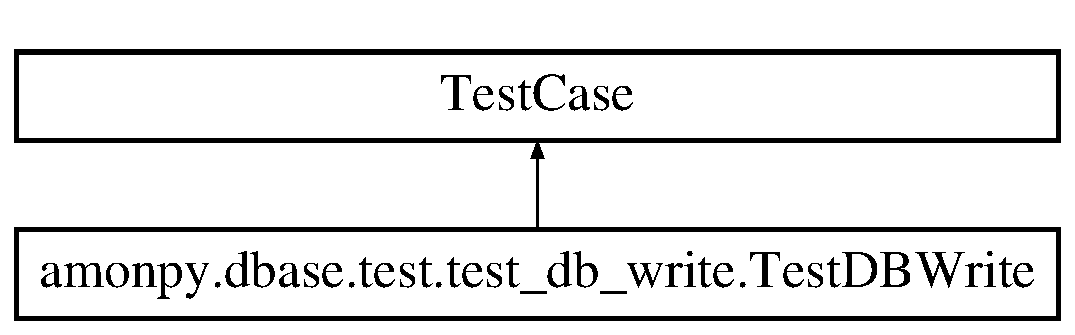
\includegraphics[height=2.000000cm]{db/d42/classamonpy_1_1dbase_1_1test_1_1test__db__write_1_1_test_d_b_write}
\end{center}
\end{figure}
\subsection*{Public Member Functions}
\begin{DoxyCompactItemize}
\item 
def \hyperlink{classamonpy_1_1dbase_1_1test_1_1test__db__write_1_1_test_d_b_write_a8ef76286fea5446138811375fb7f66b5}{set\-Up}
\item 
def \hyperlink{classamonpy_1_1dbase_1_1test_1_1test__db__write_1_1_test_d_b_write_aa32d3bef1374ed78d24d9576db67efab}{tear\-Down}
\item 
def \hyperlink{classamonpy_1_1dbase_1_1test_1_1test__db__write_1_1_test_d_b_write_a02684496f0a6f809cc60ab8873b125c8}{test\-Write\-Param\-List}
\end{DoxyCompactItemize}
\subsection*{Public Attributes}
\begin{DoxyCompactItemize}
\item 
\hyperlink{classamonpy_1_1dbase_1_1test_1_1test__db__write_1_1_test_d_b_write_a21f01f500a675067822bf868ce371306}{real\-Archive}
\item 
\hyperlink{classamonpy_1_1dbase_1_1test_1_1test__db__write_1_1_test_d_b_write_a1d99ea6d169624f39acc56254f9f7f30}{Host\-Fancy\-Name}
\item 
\hyperlink{classamonpy_1_1dbase_1_1test_1_1test__db__write_1_1_test_d_b_write_ab23c3c078c9ef84ff80e595d0906cd83}{User\-Fancy\-Name}
\item 
\hyperlink{classamonpy_1_1dbase_1_1test_1_1test__db__write_1_1_test_d_b_write_a69e2b25f75c000b814fa55d4945cd241}{Password\-Fancy}
\item 
\hyperlink{classamonpy_1_1dbase_1_1test_1_1test__db__write_1_1_test_d_b_write_a7b07a25b051063de016eaa355562eac3}{D\-B\-Fancy\-Name}
\item 
\hyperlink{classamonpy_1_1dbase_1_1test_1_1test__db__write_1_1_test_d_b_write_ad305c09b7cfbca1150be4b5819d0fdf4}{D\-B\-Fancy\-Name\-M\-C}
\item 
\hyperlink{classamonpy_1_1dbase_1_1test_1_1test__db__write_1_1_test_d_b_write_a12e956ebf3f624d6b36bb053369dd608}{Stream\-Fancy\-Name}
\item 
\hyperlink{classamonpy_1_1dbase_1_1test_1_1test__db__write_1_1_test_d_b_write_afe1cf31a726c2a34b3f8b3a5d130c3af}{Alert\-Stream\-Fancy\-Name}
\item 
\hyperlink{classamonpy_1_1dbase_1_1test_1_1test__db__write_1_1_test_d_b_write_a2096a0b2fb2fe15fcb2894f1a7d61c68}{Stream\-Fancy\-Name\-M\-C}
\item 
\hyperlink{classamonpy_1_1dbase_1_1test_1_1test__db__write_1_1_test_d_b_write_a2e1e2201ab54a4ea4eb59294ada2fd1a}{Stream\-Alert\-Config}
\item 
\hyperlink{classamonpy_1_1dbase_1_1test_1_1test__db__write_1_1_test_d_b_write_a9d4454368eabffc5e634852d7f6bf809}{Filename}
\item 
\hyperlink{classamonpy_1_1dbase_1_1test_1_1test__db__write_1_1_test_d_b_write_a23801af3747df6a10fe1e3e087f41ddc}{Sim\-Config}
\item 
\hyperlink{classamonpy_1_1dbase_1_1test_1_1test__db__write_1_1_test_d_b_write_a46fd1b5ec3c30b43fc1ba03a19603f3a}{Alert\-Config\-Single}
\item 
\hyperlink{classamonpy_1_1dbase_1_1test_1_1test__db__write_1_1_test_d_b_write_abf87a227a67042fea9ec1a8056656d77}{Alert\-Single}
\item 
\hyperlink{classamonpy_1_1dbase_1_1test_1_1test__db__write_1_1_test_d_b_write_a678e5a1daa722c397816fbcbf21aba3b}{Parameter}
\end{DoxyCompactItemize}


\subsection{Detailed Description}
Unit tests for \hyperlink{namespaceamonpy_1_1dbase_1_1db__write}{db\-\_\-write} module. 

Definition at line 16 of file test\-\_\-db\-\_\-write.\-py.



\subsection{Member Function Documentation}
\hypertarget{classamonpy_1_1dbase_1_1test_1_1test__db__write_1_1_test_d_b_write_a8ef76286fea5446138811375fb7f66b5}{\index{amonpy\-::dbase\-::test\-::test\-\_\-db\-\_\-write\-::\-Test\-D\-B\-Write@{amonpy\-::dbase\-::test\-::test\-\_\-db\-\_\-write\-::\-Test\-D\-B\-Write}!set\-Up@{set\-Up}}
\index{set\-Up@{set\-Up}!amonpy::dbase::test::test_db_write::TestDBWrite@{amonpy\-::dbase\-::test\-::test\-\_\-db\-\_\-write\-::\-Test\-D\-B\-Write}}
\subsubsection[{set\-Up}]{\setlength{\rightskip}{0pt plus 5cm}def amonpy.\-dbase.\-test.\-test\-\_\-db\-\_\-write.\-Test\-D\-B\-Write.\-set\-Up (
\begin{DoxyParamCaption}
\item[{}]{self}
\end{DoxyParamCaption}
)}}\label{classamonpy_1_1dbase_1_1test_1_1test__db__write_1_1_test_d_b_write_a8ef76286fea5446138811375fb7f66b5}


Definition at line 17 of file test\-\_\-db\-\_\-write.\-py.

\hypertarget{classamonpy_1_1dbase_1_1test_1_1test__db__write_1_1_test_d_b_write_aa32d3bef1374ed78d24d9576db67efab}{\index{amonpy\-::dbase\-::test\-::test\-\_\-db\-\_\-write\-::\-Test\-D\-B\-Write@{amonpy\-::dbase\-::test\-::test\-\_\-db\-\_\-write\-::\-Test\-D\-B\-Write}!tear\-Down@{tear\-Down}}
\index{tear\-Down@{tear\-Down}!amonpy::dbase::test::test_db_write::TestDBWrite@{amonpy\-::dbase\-::test\-::test\-\_\-db\-\_\-write\-::\-Test\-D\-B\-Write}}
\subsubsection[{tear\-Down}]{\setlength{\rightskip}{0pt plus 5cm}def amonpy.\-dbase.\-test.\-test\-\_\-db\-\_\-write.\-Test\-D\-B\-Write.\-tear\-Down (
\begin{DoxyParamCaption}
\item[{}]{self}
\end{DoxyParamCaption}
)}}\label{classamonpy_1_1dbase_1_1test_1_1test__db__write_1_1_test_d_b_write_aa32d3bef1374ed78d24d9576db67efab}


Definition at line 38 of file test\-\_\-db\-\_\-write.\-py.

\hypertarget{classamonpy_1_1dbase_1_1test_1_1test__db__write_1_1_test_d_b_write_a02684496f0a6f809cc60ab8873b125c8}{\index{amonpy\-::dbase\-::test\-::test\-\_\-db\-\_\-write\-::\-Test\-D\-B\-Write@{amonpy\-::dbase\-::test\-::test\-\_\-db\-\_\-write\-::\-Test\-D\-B\-Write}!test\-Write\-Param\-List@{test\-Write\-Param\-List}}
\index{test\-Write\-Param\-List@{test\-Write\-Param\-List}!amonpy::dbase::test::test_db_write::TestDBWrite@{amonpy\-::dbase\-::test\-::test\-\_\-db\-\_\-write\-::\-Test\-D\-B\-Write}}
\subsubsection[{test\-Write\-Param\-List}]{\setlength{\rightskip}{0pt plus 5cm}def amonpy.\-dbase.\-test.\-test\-\_\-db\-\_\-write.\-Test\-D\-B\-Write.\-test\-Write\-Param\-List (
\begin{DoxyParamCaption}
\item[{}]{self}
\end{DoxyParamCaption}
)}}\label{classamonpy_1_1dbase_1_1test_1_1test__db__write_1_1_test_d_b_write_a02684496f0a6f809cc60ab8873b125c8}


Definition at line 86 of file test\-\_\-db\-\_\-write.\-py.



\subsection{Member Data Documentation}
\hypertarget{classamonpy_1_1dbase_1_1test_1_1test__db__write_1_1_test_d_b_write_a46fd1b5ec3c30b43fc1ba03a19603f3a}{\index{amonpy\-::dbase\-::test\-::test\-\_\-db\-\_\-write\-::\-Test\-D\-B\-Write@{amonpy\-::dbase\-::test\-::test\-\_\-db\-\_\-write\-::\-Test\-D\-B\-Write}!Alert\-Config\-Single@{Alert\-Config\-Single}}
\index{Alert\-Config\-Single@{Alert\-Config\-Single}!amonpy::dbase::test::test_db_write::TestDBWrite@{amonpy\-::dbase\-::test\-::test\-\_\-db\-\_\-write\-::\-Test\-D\-B\-Write}}
\subsubsection[{Alert\-Config\-Single}]{\setlength{\rightskip}{0pt plus 5cm}amonpy.\-dbase.\-test.\-test\-\_\-db\-\_\-write.\-Test\-D\-B\-Write.\-Alert\-Config\-Single}}\label{classamonpy_1_1dbase_1_1test_1_1test__db__write_1_1_test_d_b_write_a46fd1b5ec3c30b43fc1ba03a19603f3a}


Definition at line 32 of file test\-\_\-db\-\_\-write.\-py.

\hypertarget{classamonpy_1_1dbase_1_1test_1_1test__db__write_1_1_test_d_b_write_abf87a227a67042fea9ec1a8056656d77}{\index{amonpy\-::dbase\-::test\-::test\-\_\-db\-\_\-write\-::\-Test\-D\-B\-Write@{amonpy\-::dbase\-::test\-::test\-\_\-db\-\_\-write\-::\-Test\-D\-B\-Write}!Alert\-Single@{Alert\-Single}}
\index{Alert\-Single@{Alert\-Single}!amonpy::dbase::test::test_db_write::TestDBWrite@{amonpy\-::dbase\-::test\-::test\-\_\-db\-\_\-write\-::\-Test\-D\-B\-Write}}
\subsubsection[{Alert\-Single}]{\setlength{\rightskip}{0pt plus 5cm}amonpy.\-dbase.\-test.\-test\-\_\-db\-\_\-write.\-Test\-D\-B\-Write.\-Alert\-Single}}\label{classamonpy_1_1dbase_1_1test_1_1test__db__write_1_1_test_d_b_write_abf87a227a67042fea9ec1a8056656d77}


Definition at line 33 of file test\-\_\-db\-\_\-write.\-py.

\hypertarget{classamonpy_1_1dbase_1_1test_1_1test__db__write_1_1_test_d_b_write_afe1cf31a726c2a34b3f8b3a5d130c3af}{\index{amonpy\-::dbase\-::test\-::test\-\_\-db\-\_\-write\-::\-Test\-D\-B\-Write@{amonpy\-::dbase\-::test\-::test\-\_\-db\-\_\-write\-::\-Test\-D\-B\-Write}!Alert\-Stream\-Fancy\-Name@{Alert\-Stream\-Fancy\-Name}}
\index{Alert\-Stream\-Fancy\-Name@{Alert\-Stream\-Fancy\-Name}!amonpy::dbase::test::test_db_write::TestDBWrite@{amonpy\-::dbase\-::test\-::test\-\_\-db\-\_\-write\-::\-Test\-D\-B\-Write}}
\subsubsection[{Alert\-Stream\-Fancy\-Name}]{\setlength{\rightskip}{0pt plus 5cm}amonpy.\-dbase.\-test.\-test\-\_\-db\-\_\-write.\-Test\-D\-B\-Write.\-Alert\-Stream\-Fancy\-Name}}\label{classamonpy_1_1dbase_1_1test_1_1test__db__write_1_1_test_d_b_write_afe1cf31a726c2a34b3f8b3a5d130c3af}


Definition at line 26 of file test\-\_\-db\-\_\-write.\-py.

\hypertarget{classamonpy_1_1dbase_1_1test_1_1test__db__write_1_1_test_d_b_write_a7b07a25b051063de016eaa355562eac3}{\index{amonpy\-::dbase\-::test\-::test\-\_\-db\-\_\-write\-::\-Test\-D\-B\-Write@{amonpy\-::dbase\-::test\-::test\-\_\-db\-\_\-write\-::\-Test\-D\-B\-Write}!D\-B\-Fancy\-Name@{D\-B\-Fancy\-Name}}
\index{D\-B\-Fancy\-Name@{D\-B\-Fancy\-Name}!amonpy::dbase::test::test_db_write::TestDBWrite@{amonpy\-::dbase\-::test\-::test\-\_\-db\-\_\-write\-::\-Test\-D\-B\-Write}}
\subsubsection[{D\-B\-Fancy\-Name}]{\setlength{\rightskip}{0pt plus 5cm}amonpy.\-dbase.\-test.\-test\-\_\-db\-\_\-write.\-Test\-D\-B\-Write.\-D\-B\-Fancy\-Name}}\label{classamonpy_1_1dbase_1_1test_1_1test__db__write_1_1_test_d_b_write_a7b07a25b051063de016eaa355562eac3}


Definition at line 23 of file test\-\_\-db\-\_\-write.\-py.

\hypertarget{classamonpy_1_1dbase_1_1test_1_1test__db__write_1_1_test_d_b_write_ad305c09b7cfbca1150be4b5819d0fdf4}{\index{amonpy\-::dbase\-::test\-::test\-\_\-db\-\_\-write\-::\-Test\-D\-B\-Write@{amonpy\-::dbase\-::test\-::test\-\_\-db\-\_\-write\-::\-Test\-D\-B\-Write}!D\-B\-Fancy\-Name\-M\-C@{D\-B\-Fancy\-Name\-M\-C}}
\index{D\-B\-Fancy\-Name\-M\-C@{D\-B\-Fancy\-Name\-M\-C}!amonpy::dbase::test::test_db_write::TestDBWrite@{amonpy\-::dbase\-::test\-::test\-\_\-db\-\_\-write\-::\-Test\-D\-B\-Write}}
\subsubsection[{D\-B\-Fancy\-Name\-M\-C}]{\setlength{\rightskip}{0pt plus 5cm}amonpy.\-dbase.\-test.\-test\-\_\-db\-\_\-write.\-Test\-D\-B\-Write.\-D\-B\-Fancy\-Name\-M\-C}}\label{classamonpy_1_1dbase_1_1test_1_1test__db__write_1_1_test_d_b_write_ad305c09b7cfbca1150be4b5819d0fdf4}


Definition at line 24 of file test\-\_\-db\-\_\-write.\-py.

\hypertarget{classamonpy_1_1dbase_1_1test_1_1test__db__write_1_1_test_d_b_write_a9d4454368eabffc5e634852d7f6bf809}{\index{amonpy\-::dbase\-::test\-::test\-\_\-db\-\_\-write\-::\-Test\-D\-B\-Write@{amonpy\-::dbase\-::test\-::test\-\_\-db\-\_\-write\-::\-Test\-D\-B\-Write}!Filename@{Filename}}
\index{Filename@{Filename}!amonpy::dbase::test::test_db_write::TestDBWrite@{amonpy\-::dbase\-::test\-::test\-\_\-db\-\_\-write\-::\-Test\-D\-B\-Write}}
\subsubsection[{Filename}]{\setlength{\rightskip}{0pt plus 5cm}amonpy.\-dbase.\-test.\-test\-\_\-db\-\_\-write.\-Test\-D\-B\-Write.\-Filename}}\label{classamonpy_1_1dbase_1_1test_1_1test__db__write_1_1_test_d_b_write_a9d4454368eabffc5e634852d7f6bf809}


Definition at line 29 of file test\-\_\-db\-\_\-write.\-py.

\hypertarget{classamonpy_1_1dbase_1_1test_1_1test__db__write_1_1_test_d_b_write_a1d99ea6d169624f39acc56254f9f7f30}{\index{amonpy\-::dbase\-::test\-::test\-\_\-db\-\_\-write\-::\-Test\-D\-B\-Write@{amonpy\-::dbase\-::test\-::test\-\_\-db\-\_\-write\-::\-Test\-D\-B\-Write}!Host\-Fancy\-Name@{Host\-Fancy\-Name}}
\index{Host\-Fancy\-Name@{Host\-Fancy\-Name}!amonpy::dbase::test::test_db_write::TestDBWrite@{amonpy\-::dbase\-::test\-::test\-\_\-db\-\_\-write\-::\-Test\-D\-B\-Write}}
\subsubsection[{Host\-Fancy\-Name}]{\setlength{\rightskip}{0pt plus 5cm}amonpy.\-dbase.\-test.\-test\-\_\-db\-\_\-write.\-Test\-D\-B\-Write.\-Host\-Fancy\-Name}}\label{classamonpy_1_1dbase_1_1test_1_1test__db__write_1_1_test_d_b_write_a1d99ea6d169624f39acc56254f9f7f30}


Definition at line 20 of file test\-\_\-db\-\_\-write.\-py.

\hypertarget{classamonpy_1_1dbase_1_1test_1_1test__db__write_1_1_test_d_b_write_a678e5a1daa722c397816fbcbf21aba3b}{\index{amonpy\-::dbase\-::test\-::test\-\_\-db\-\_\-write\-::\-Test\-D\-B\-Write@{amonpy\-::dbase\-::test\-::test\-\_\-db\-\_\-write\-::\-Test\-D\-B\-Write}!Parameter@{Parameter}}
\index{Parameter@{Parameter}!amonpy::dbase::test::test_db_write::TestDBWrite@{amonpy\-::dbase\-::test\-::test\-\_\-db\-\_\-write\-::\-Test\-D\-B\-Write}}
\subsubsection[{Parameter}]{\setlength{\rightskip}{0pt plus 5cm}amonpy.\-dbase.\-test.\-test\-\_\-db\-\_\-write.\-Test\-D\-B\-Write.\-Parameter}}\label{classamonpy_1_1dbase_1_1test_1_1test__db__write_1_1_test_d_b_write_a678e5a1daa722c397816fbcbf21aba3b}


Definition at line 34 of file test\-\_\-db\-\_\-write.\-py.

\hypertarget{classamonpy_1_1dbase_1_1test_1_1test__db__write_1_1_test_d_b_write_a69e2b25f75c000b814fa55d4945cd241}{\index{amonpy\-::dbase\-::test\-::test\-\_\-db\-\_\-write\-::\-Test\-D\-B\-Write@{amonpy\-::dbase\-::test\-::test\-\_\-db\-\_\-write\-::\-Test\-D\-B\-Write}!Password\-Fancy@{Password\-Fancy}}
\index{Password\-Fancy@{Password\-Fancy}!amonpy::dbase::test::test_db_write::TestDBWrite@{amonpy\-::dbase\-::test\-::test\-\_\-db\-\_\-write\-::\-Test\-D\-B\-Write}}
\subsubsection[{Password\-Fancy}]{\setlength{\rightskip}{0pt plus 5cm}amonpy.\-dbase.\-test.\-test\-\_\-db\-\_\-write.\-Test\-D\-B\-Write.\-Password\-Fancy}}\label{classamonpy_1_1dbase_1_1test_1_1test__db__write_1_1_test_d_b_write_a69e2b25f75c000b814fa55d4945cd241}


Definition at line 22 of file test\-\_\-db\-\_\-write.\-py.

\hypertarget{classamonpy_1_1dbase_1_1test_1_1test__db__write_1_1_test_d_b_write_a21f01f500a675067822bf868ce371306}{\index{amonpy\-::dbase\-::test\-::test\-\_\-db\-\_\-write\-::\-Test\-D\-B\-Write@{amonpy\-::dbase\-::test\-::test\-\_\-db\-\_\-write\-::\-Test\-D\-B\-Write}!real\-Archive@{real\-Archive}}
\index{real\-Archive@{real\-Archive}!amonpy::dbase::test::test_db_write::TestDBWrite@{amonpy\-::dbase\-::test\-::test\-\_\-db\-\_\-write\-::\-Test\-D\-B\-Write}}
\subsubsection[{real\-Archive}]{\setlength{\rightskip}{0pt plus 5cm}amonpy.\-dbase.\-test.\-test\-\_\-db\-\_\-write.\-Test\-D\-B\-Write.\-real\-Archive}}\label{classamonpy_1_1dbase_1_1test_1_1test__db__write_1_1_test_d_b_write_a21f01f500a675067822bf868ce371306}


Definition at line 19 of file test\-\_\-db\-\_\-write.\-py.

\hypertarget{classamonpy_1_1dbase_1_1test_1_1test__db__write_1_1_test_d_b_write_a23801af3747df6a10fe1e3e087f41ddc}{\index{amonpy\-::dbase\-::test\-::test\-\_\-db\-\_\-write\-::\-Test\-D\-B\-Write@{amonpy\-::dbase\-::test\-::test\-\_\-db\-\_\-write\-::\-Test\-D\-B\-Write}!Sim\-Config@{Sim\-Config}}
\index{Sim\-Config@{Sim\-Config}!amonpy::dbase::test::test_db_write::TestDBWrite@{amonpy\-::dbase\-::test\-::test\-\_\-db\-\_\-write\-::\-Test\-D\-B\-Write}}
\subsubsection[{Sim\-Config}]{\setlength{\rightskip}{0pt plus 5cm}amonpy.\-dbase.\-test.\-test\-\_\-db\-\_\-write.\-Test\-D\-B\-Write.\-Sim\-Config}}\label{classamonpy_1_1dbase_1_1test_1_1test__db__write_1_1_test_d_b_write_a23801af3747df6a10fe1e3e087f41ddc}


Definition at line 30 of file test\-\_\-db\-\_\-write.\-py.

\hypertarget{classamonpy_1_1dbase_1_1test_1_1test__db__write_1_1_test_d_b_write_a2e1e2201ab54a4ea4eb59294ada2fd1a}{\index{amonpy\-::dbase\-::test\-::test\-\_\-db\-\_\-write\-::\-Test\-D\-B\-Write@{amonpy\-::dbase\-::test\-::test\-\_\-db\-\_\-write\-::\-Test\-D\-B\-Write}!Stream\-Alert\-Config@{Stream\-Alert\-Config}}
\index{Stream\-Alert\-Config@{Stream\-Alert\-Config}!amonpy::dbase::test::test_db_write::TestDBWrite@{amonpy\-::dbase\-::test\-::test\-\_\-db\-\_\-write\-::\-Test\-D\-B\-Write}}
\subsubsection[{Stream\-Alert\-Config}]{\setlength{\rightskip}{0pt plus 5cm}amonpy.\-dbase.\-test.\-test\-\_\-db\-\_\-write.\-Test\-D\-B\-Write.\-Stream\-Alert\-Config}}\label{classamonpy_1_1dbase_1_1test_1_1test__db__write_1_1_test_d_b_write_a2e1e2201ab54a4ea4eb59294ada2fd1a}


Definition at line 28 of file test\-\_\-db\-\_\-write.\-py.

\hypertarget{classamonpy_1_1dbase_1_1test_1_1test__db__write_1_1_test_d_b_write_a12e956ebf3f624d6b36bb053369dd608}{\index{amonpy\-::dbase\-::test\-::test\-\_\-db\-\_\-write\-::\-Test\-D\-B\-Write@{amonpy\-::dbase\-::test\-::test\-\_\-db\-\_\-write\-::\-Test\-D\-B\-Write}!Stream\-Fancy\-Name@{Stream\-Fancy\-Name}}
\index{Stream\-Fancy\-Name@{Stream\-Fancy\-Name}!amonpy::dbase::test::test_db_write::TestDBWrite@{amonpy\-::dbase\-::test\-::test\-\_\-db\-\_\-write\-::\-Test\-D\-B\-Write}}
\subsubsection[{Stream\-Fancy\-Name}]{\setlength{\rightskip}{0pt plus 5cm}amonpy.\-dbase.\-test.\-test\-\_\-db\-\_\-write.\-Test\-D\-B\-Write.\-Stream\-Fancy\-Name}}\label{classamonpy_1_1dbase_1_1test_1_1test__db__write_1_1_test_d_b_write_a12e956ebf3f624d6b36bb053369dd608}


Definition at line 25 of file test\-\_\-db\-\_\-write.\-py.

\hypertarget{classamonpy_1_1dbase_1_1test_1_1test__db__write_1_1_test_d_b_write_a2096a0b2fb2fe15fcb2894f1a7d61c68}{\index{amonpy\-::dbase\-::test\-::test\-\_\-db\-\_\-write\-::\-Test\-D\-B\-Write@{amonpy\-::dbase\-::test\-::test\-\_\-db\-\_\-write\-::\-Test\-D\-B\-Write}!Stream\-Fancy\-Name\-M\-C@{Stream\-Fancy\-Name\-M\-C}}
\index{Stream\-Fancy\-Name\-M\-C@{Stream\-Fancy\-Name\-M\-C}!amonpy::dbase::test::test_db_write::TestDBWrite@{amonpy\-::dbase\-::test\-::test\-\_\-db\-\_\-write\-::\-Test\-D\-B\-Write}}
\subsubsection[{Stream\-Fancy\-Name\-M\-C}]{\setlength{\rightskip}{0pt plus 5cm}amonpy.\-dbase.\-test.\-test\-\_\-db\-\_\-write.\-Test\-D\-B\-Write.\-Stream\-Fancy\-Name\-M\-C}}\label{classamonpy_1_1dbase_1_1test_1_1test__db__write_1_1_test_d_b_write_a2096a0b2fb2fe15fcb2894f1a7d61c68}


Definition at line 27 of file test\-\_\-db\-\_\-write.\-py.

\hypertarget{classamonpy_1_1dbase_1_1test_1_1test__db__write_1_1_test_d_b_write_ab23c3c078c9ef84ff80e595d0906cd83}{\index{amonpy\-::dbase\-::test\-::test\-\_\-db\-\_\-write\-::\-Test\-D\-B\-Write@{amonpy\-::dbase\-::test\-::test\-\_\-db\-\_\-write\-::\-Test\-D\-B\-Write}!User\-Fancy\-Name@{User\-Fancy\-Name}}
\index{User\-Fancy\-Name@{User\-Fancy\-Name}!amonpy::dbase::test::test_db_write::TestDBWrite@{amonpy\-::dbase\-::test\-::test\-\_\-db\-\_\-write\-::\-Test\-D\-B\-Write}}
\subsubsection[{User\-Fancy\-Name}]{\setlength{\rightskip}{0pt plus 5cm}amonpy.\-dbase.\-test.\-test\-\_\-db\-\_\-write.\-Test\-D\-B\-Write.\-User\-Fancy\-Name}}\label{classamonpy_1_1dbase_1_1test_1_1test__db__write_1_1_test_d_b_write_ab23c3c078c9ef84ff80e595d0906cd83}


Definition at line 21 of file test\-\_\-db\-\_\-write.\-py.



The documentation for this class was generated from the following file\-:\begin{DoxyCompactItemize}
\item 
amonpy/dbase/test/\hyperlink{test__db__write_8py}{test\-\_\-db\-\_\-write.\-py}\end{DoxyCompactItemize}

\hypertarget{classtest__sidereal_1_1_test_sidereal}{\section{test\-\_\-sidereal.\-Test\-Sidereal Class Reference}
\label{classtest__sidereal_1_1_test_sidereal}\index{test\-\_\-sidereal.\-Test\-Sidereal@{test\-\_\-sidereal.\-Test\-Sidereal}}
}
Inheritance diagram for test\-\_\-sidereal.\-Test\-Sidereal\-:\begin{figure}[H]
\begin{center}
\leavevmode
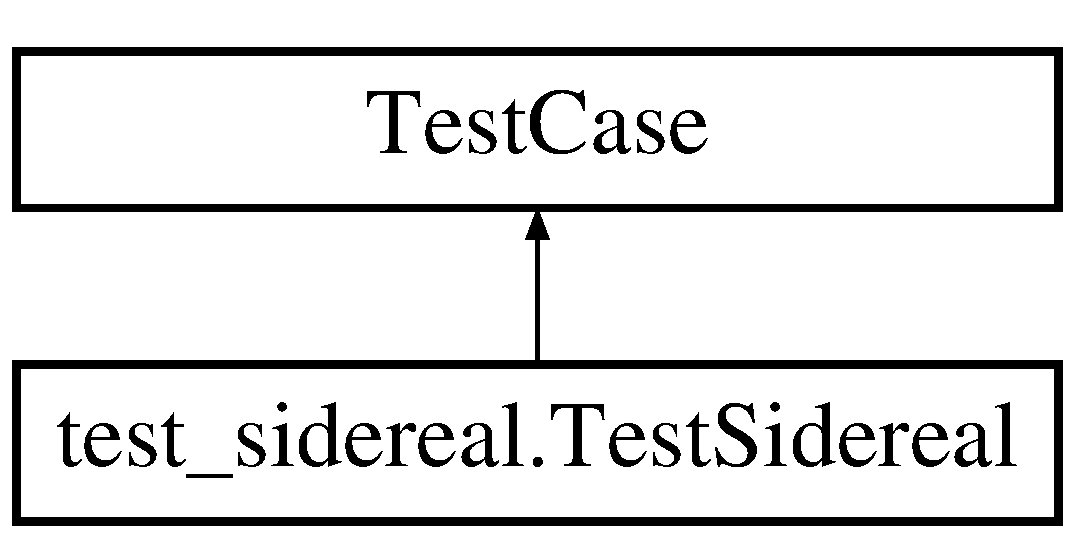
\includegraphics[height=2.000000cm]{classtest__sidereal_1_1_test_sidereal}
\end{center}
\end{figure}
\subsection*{Public Member Functions}
\begin{DoxyCompactItemize}
\item 
def \hyperlink{classtest__sidereal_1_1_test_sidereal_a63b312fe76d9023b2b0cf40045929e90}{set\-Up}
\item 
def \hyperlink{classtest__sidereal_1_1_test_sidereal_a1a26249915d94355c6ea0a21d917a96b}{tear\-Down}
\item 
def \hyperlink{classtest__sidereal_1_1_test_sidereal_adbdd8a1fa36785c878bddea37ad5b8ec}{test1\-\_\-coords}
\end{DoxyCompactItemize}


\subsection{Member Function Documentation}
\hypertarget{classtest__sidereal_1_1_test_sidereal_a63b312fe76d9023b2b0cf40045929e90}{\index{test\-\_\-sidereal\-::\-Test\-Sidereal@{test\-\_\-sidereal\-::\-Test\-Sidereal}!set\-Up@{set\-Up}}
\index{set\-Up@{set\-Up}!test_sidereal::TestSidereal@{test\-\_\-sidereal\-::\-Test\-Sidereal}}
\subsubsection[{set\-Up}]{\setlength{\rightskip}{0pt plus 5cm}def test\-\_\-sidereal.\-Test\-Sidereal.\-set\-Up (
\begin{DoxyParamCaption}
\item[{}]{self}
\end{DoxyParamCaption}
)}}\label{classtest__sidereal_1_1_test_sidereal_a63b312fe76d9023b2b0cf40045929e90}
\hypertarget{classtest__sidereal_1_1_test_sidereal_a1a26249915d94355c6ea0a21d917a96b}{\index{test\-\_\-sidereal\-::\-Test\-Sidereal@{test\-\_\-sidereal\-::\-Test\-Sidereal}!tear\-Down@{tear\-Down}}
\index{tear\-Down@{tear\-Down}!test_sidereal::TestSidereal@{test\-\_\-sidereal\-::\-Test\-Sidereal}}
\subsubsection[{tear\-Down}]{\setlength{\rightskip}{0pt plus 5cm}def test\-\_\-sidereal.\-Test\-Sidereal.\-tear\-Down (
\begin{DoxyParamCaption}
\item[{}]{self}
\end{DoxyParamCaption}
)}}\label{classtest__sidereal_1_1_test_sidereal_a1a26249915d94355c6ea0a21d917a96b}
\hypertarget{classtest__sidereal_1_1_test_sidereal_adbdd8a1fa36785c878bddea37ad5b8ec}{\index{test\-\_\-sidereal\-::\-Test\-Sidereal@{test\-\_\-sidereal\-::\-Test\-Sidereal}!test1\-\_\-coords@{test1\-\_\-coords}}
\index{test1\-\_\-coords@{test1\-\_\-coords}!test_sidereal::TestSidereal@{test\-\_\-sidereal\-::\-Test\-Sidereal}}
\subsubsection[{test1\-\_\-coords}]{\setlength{\rightskip}{0pt plus 5cm}def test\-\_\-sidereal.\-Test\-Sidereal.\-test1\-\_\-coords (
\begin{DoxyParamCaption}
\item[{}]{self}
\end{DoxyParamCaption}
)}}\label{classtest__sidereal_1_1_test_sidereal_adbdd8a1fa36785c878bddea37ad5b8ec}


The documentation for this class was generated from the following file\-:\begin{DoxyCompactItemize}
\item 
amonpy/sim/test/\hyperlink{test__sidereal_8py}{test\-\_\-sidereal.\-py}\end{DoxyCompactItemize}

\hypertarget{classgrbsim_1_1_universe}{\section{grbsim.\-Universe Class Reference}
\label{classgrbsim_1_1_universe}\index{grbsim.\-Universe@{grbsim.\-Universe}}
}


\hyperlink{classgrbsim_1_1_universe}{Universe} Class \#\#\#\#\#\#\#\#\#\#\#\#\#\#\#\#.  


Inheritance diagram for grbsim.\-Universe\-:\begin{figure}[H]
\begin{center}
\leavevmode
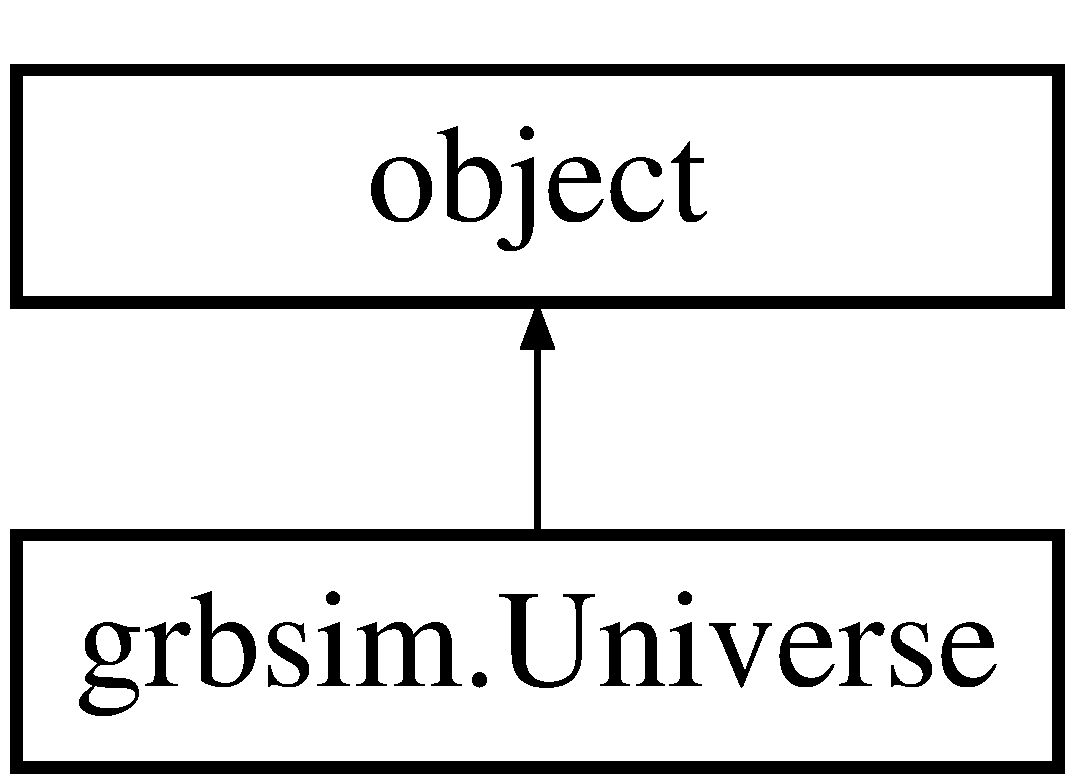
\includegraphics[height=2.000000cm]{d2/ddc/classgrbsim_1_1_universe}
\end{center}
\end{figure}
\subsection*{Public Member Functions}
\begin{DoxyCompactItemize}
\item 
def \hyperlink{classgrbsim_1_1_universe_a477782a9799e593606c8b93e32979575}{\-\_\-\-\_\-init\-\_\-\-\_\-}
\item 
def \hyperlink{classgrbsim_1_1_universe_a1ee331ee5b8c47d649975c1b830cb97a}{D\-\_\-\-H}
\item 
def \hyperlink{classgrbsim_1_1_universe_af182961238cc8a6cf74f967ace71fac3}{E}
\item 
def \hyperlink{classgrbsim_1_1_universe_a1520f08536b821def06948b39cf18427}{g}
\item 
def \hyperlink{classgrbsim_1_1_universe_afd74ef68d25363c13f2c94e96b2a8a8d}{D\-\_\-\-C}
\item 
def \hyperlink{classgrbsim_1_1_universe_ac6e2184d18fb119538df164a647fe13b}{D\-\_\-\-M}
\item 
def \hyperlink{classgrbsim_1_1_universe_a09d15f75aedac6a8b1375ac233b8c247}{D\-\_\-\-L}
\item 
def \hyperlink{classgrbsim_1_1_universe_ad58fe82edeb3e353f6eb9012f6c35ac0}{D\-\_\-\-A}
\item 
def \hyperlink{classgrbsim_1_1_universe_ac7ba7d8a9e9cd0c6fe8ce792e939752c}{d\-V\-\_\-dz}
\end{DoxyCompactItemize}
\subsection*{Public Attributes}
\begin{DoxyCompactItemize}
\item 
\hyperlink{classgrbsim_1_1_universe_a59f1abb2ade1948560357a1fd28bbaeb}{h}
\item 
\hyperlink{classgrbsim_1_1_universe_a50a43043c5dd268cba4242c241b730b4}{omegam}
\item 
\hyperlink{classgrbsim_1_1_universe_a70b693aecf5f78246da8652a9f8f8cc9}{omegak}
\item 
\hyperlink{classgrbsim_1_1_universe_a84f0d8f958e91a15d3a88263df6dbdeb}{omegae}
\item 
\hyperlink{classgrbsim_1_1_universe_ad5dd40bbc7e6a2371cf1515b4fa3d59f}{c}
\item 
\hyperlink{classgrbsim_1_1_universe_a0510b25f83d19c1573caa988326f35e5}{Mpc2cm}
\item 
\hyperlink{classgrbsim_1_1_universe_afc9d348bf0da237becec80a8ba758121}{erg2\-Me\-V}
\end{DoxyCompactItemize}


\subsection{Detailed Description}
\hyperlink{classgrbsim_1_1_universe}{Universe} Class \#\#\#\#\#\#\#\#\#\#\#\#\#\#\#\#. 

Definition at line 7 of file grbsim.\-py.



\subsection{Constructor \& Destructor Documentation}
\hypertarget{classgrbsim_1_1_universe_a477782a9799e593606c8b93e32979575}{\index{grbsim\-::\-Universe@{grbsim\-::\-Universe}!\-\_\-\-\_\-init\-\_\-\-\_\-@{\-\_\-\-\_\-init\-\_\-\-\_\-}}
\index{\-\_\-\-\_\-init\-\_\-\-\_\-@{\-\_\-\-\_\-init\-\_\-\-\_\-}!grbsim::Universe@{grbsim\-::\-Universe}}
\subsubsection[{\-\_\-\-\_\-init\-\_\-\-\_\-}]{\setlength{\rightskip}{0pt plus 5cm}def grbsim.\-Universe.\-\_\-\-\_\-init\-\_\-\-\_\- (
\begin{DoxyParamCaption}
\item[{}]{self, }
\item[{}]{h, }
\item[{}]{omegam, }
\item[{}]{omegak, }
\item[{}]{omegae}
\end{DoxyParamCaption}
)}}\label{classgrbsim_1_1_universe_a477782a9799e593606c8b93e32979575}


Definition at line 8 of file grbsim.\-py.



\subsection{Member Function Documentation}
\hypertarget{classgrbsim_1_1_universe_ad58fe82edeb3e353f6eb9012f6c35ac0}{\index{grbsim\-::\-Universe@{grbsim\-::\-Universe}!D\-\_\-\-A@{D\-\_\-\-A}}
\index{D\-\_\-\-A@{D\-\_\-\-A}!grbsim::Universe@{grbsim\-::\-Universe}}
\subsubsection[{D\-\_\-\-A}]{\setlength{\rightskip}{0pt plus 5cm}def grbsim.\-Universe.\-D\-\_\-\-A (
\begin{DoxyParamCaption}
\item[{}]{self, }
\item[{}]{z}
\end{DoxyParamCaption}
)}}\label{classgrbsim_1_1_universe_ad58fe82edeb3e353f6eb9012f6c35ac0}


Definition at line 53 of file grbsim.\-py.

\hypertarget{classgrbsim_1_1_universe_afd74ef68d25363c13f2c94e96b2a8a8d}{\index{grbsim\-::\-Universe@{grbsim\-::\-Universe}!D\-\_\-\-C@{D\-\_\-\-C}}
\index{D\-\_\-\-C@{D\-\_\-\-C}!grbsim::Universe@{grbsim\-::\-Universe}}
\subsubsection[{D\-\_\-\-C}]{\setlength{\rightskip}{0pt plus 5cm}def grbsim.\-Universe.\-D\-\_\-\-C (
\begin{DoxyParamCaption}
\item[{}]{self, }
\item[{}]{z}
\end{DoxyParamCaption}
)}}\label{classgrbsim_1_1_universe_afd74ef68d25363c13f2c94e96b2a8a8d}


Definition at line 31 of file grbsim.\-py.

\hypertarget{classgrbsim_1_1_universe_a1ee331ee5b8c47d649975c1b830cb97a}{\index{grbsim\-::\-Universe@{grbsim\-::\-Universe}!D\-\_\-\-H@{D\-\_\-\-H}}
\index{D\-\_\-\-H@{D\-\_\-\-H}!grbsim::Universe@{grbsim\-::\-Universe}}
\subsubsection[{D\-\_\-\-H}]{\setlength{\rightskip}{0pt plus 5cm}def grbsim.\-Universe.\-D\-\_\-\-H (
\begin{DoxyParamCaption}
\item[{}]{self}
\end{DoxyParamCaption}
)}}\label{classgrbsim_1_1_universe_a1ee331ee5b8c47d649975c1b830cb97a}


Definition at line 19 of file grbsim.\-py.

\hypertarget{classgrbsim_1_1_universe_a09d15f75aedac6a8b1375ac233b8c247}{\index{grbsim\-::\-Universe@{grbsim\-::\-Universe}!D\-\_\-\-L@{D\-\_\-\-L}}
\index{D\-\_\-\-L@{D\-\_\-\-L}!grbsim::Universe@{grbsim\-::\-Universe}}
\subsubsection[{D\-\_\-\-L}]{\setlength{\rightskip}{0pt plus 5cm}def grbsim.\-Universe.\-D\-\_\-\-L (
\begin{DoxyParamCaption}
\item[{}]{self, }
\item[{}]{z}
\end{DoxyParamCaption}
)}}\label{classgrbsim_1_1_universe_a09d15f75aedac6a8b1375ac233b8c247}


Definition at line 49 of file grbsim.\-py.

\hypertarget{classgrbsim_1_1_universe_ac6e2184d18fb119538df164a647fe13b}{\index{grbsim\-::\-Universe@{grbsim\-::\-Universe}!D\-\_\-\-M@{D\-\_\-\-M}}
\index{D\-\_\-\-M@{D\-\_\-\-M}!grbsim::Universe@{grbsim\-::\-Universe}}
\subsubsection[{D\-\_\-\-M}]{\setlength{\rightskip}{0pt plus 5cm}def grbsim.\-Universe.\-D\-\_\-\-M (
\begin{DoxyParamCaption}
\item[{}]{self, }
\item[{}]{z}
\end{DoxyParamCaption}
)}}\label{classgrbsim_1_1_universe_ac6e2184d18fb119538df164a647fe13b}


Definition at line 36 of file grbsim.\-py.

\hypertarget{classgrbsim_1_1_universe_ac7ba7d8a9e9cd0c6fe8ce792e939752c}{\index{grbsim\-::\-Universe@{grbsim\-::\-Universe}!d\-V\-\_\-dz@{d\-V\-\_\-dz}}
\index{d\-V\-\_\-dz@{d\-V\-\_\-dz}!grbsim::Universe@{grbsim\-::\-Universe}}
\subsubsection[{d\-V\-\_\-dz}]{\setlength{\rightskip}{0pt plus 5cm}def grbsim.\-Universe.\-d\-V\-\_\-dz (
\begin{DoxyParamCaption}
\item[{}]{self, }
\item[{}]{z}
\end{DoxyParamCaption}
)}}\label{classgrbsim_1_1_universe_ac7ba7d8a9e9cd0c6fe8ce792e939752c}


Definition at line 57 of file grbsim.\-py.

\hypertarget{classgrbsim_1_1_universe_af182961238cc8a6cf74f967ace71fac3}{\index{grbsim\-::\-Universe@{grbsim\-::\-Universe}!E@{E}}
\index{E@{E}!grbsim::Universe@{grbsim\-::\-Universe}}
\subsubsection[{E}]{\setlength{\rightskip}{0pt plus 5cm}def grbsim.\-Universe.\-E (
\begin{DoxyParamCaption}
\item[{}]{self, }
\item[{}]{z}
\end{DoxyParamCaption}
)}}\label{classgrbsim_1_1_universe_af182961238cc8a6cf74f967ace71fac3}


Definition at line 25 of file grbsim.\-py.

\hypertarget{classgrbsim_1_1_universe_a1520f08536b821def06948b39cf18427}{\index{grbsim\-::\-Universe@{grbsim\-::\-Universe}!g@{g}}
\index{g@{g}!grbsim::Universe@{grbsim\-::\-Universe}}
\subsubsection[{g}]{\setlength{\rightskip}{0pt plus 5cm}def grbsim.\-Universe.\-g (
\begin{DoxyParamCaption}
\item[{}]{self, }
\item[{}]{z}
\end{DoxyParamCaption}
)}}\label{classgrbsim_1_1_universe_a1520f08536b821def06948b39cf18427}


Definition at line 27 of file grbsim.\-py.



\subsection{Member Data Documentation}
\hypertarget{classgrbsim_1_1_universe_ad5dd40bbc7e6a2371cf1515b4fa3d59f}{\index{grbsim\-::\-Universe@{grbsim\-::\-Universe}!c@{c}}
\index{c@{c}!grbsim::Universe@{grbsim\-::\-Universe}}
\subsubsection[{c}]{\setlength{\rightskip}{0pt plus 5cm}grbsim.\-Universe.\-c}}\label{classgrbsim_1_1_universe_ad5dd40bbc7e6a2371cf1515b4fa3d59f}


Definition at line 13 of file grbsim.\-py.

\hypertarget{classgrbsim_1_1_universe_afc9d348bf0da237becec80a8ba758121}{\index{grbsim\-::\-Universe@{grbsim\-::\-Universe}!erg2\-Me\-V@{erg2\-Me\-V}}
\index{erg2\-Me\-V@{erg2\-Me\-V}!grbsim::Universe@{grbsim\-::\-Universe}}
\subsubsection[{erg2\-Me\-V}]{\setlength{\rightskip}{0pt plus 5cm}grbsim.\-Universe.\-erg2\-Me\-V}}\label{classgrbsim_1_1_universe_afc9d348bf0da237becec80a8ba758121}


Definition at line 15 of file grbsim.\-py.

\hypertarget{classgrbsim_1_1_universe_a59f1abb2ade1948560357a1fd28bbaeb}{\index{grbsim\-::\-Universe@{grbsim\-::\-Universe}!h@{h}}
\index{h@{h}!grbsim::Universe@{grbsim\-::\-Universe}}
\subsubsection[{h}]{\setlength{\rightskip}{0pt plus 5cm}grbsim.\-Universe.\-h}}\label{classgrbsim_1_1_universe_a59f1abb2ade1948560357a1fd28bbaeb}


Definition at line 9 of file grbsim.\-py.

\hypertarget{classgrbsim_1_1_universe_a0510b25f83d19c1573caa988326f35e5}{\index{grbsim\-::\-Universe@{grbsim\-::\-Universe}!Mpc2cm@{Mpc2cm}}
\index{Mpc2cm@{Mpc2cm}!grbsim::Universe@{grbsim\-::\-Universe}}
\subsubsection[{Mpc2cm}]{\setlength{\rightskip}{0pt plus 5cm}grbsim.\-Universe.\-Mpc2cm}}\label{classgrbsim_1_1_universe_a0510b25f83d19c1573caa988326f35e5}


Definition at line 14 of file grbsim.\-py.

\hypertarget{classgrbsim_1_1_universe_a84f0d8f958e91a15d3a88263df6dbdeb}{\index{grbsim\-::\-Universe@{grbsim\-::\-Universe}!omegae@{omegae}}
\index{omegae@{omegae}!grbsim::Universe@{grbsim\-::\-Universe}}
\subsubsection[{omegae}]{\setlength{\rightskip}{0pt plus 5cm}grbsim.\-Universe.\-omegae}}\label{classgrbsim_1_1_universe_a84f0d8f958e91a15d3a88263df6dbdeb}


Definition at line 12 of file grbsim.\-py.

\hypertarget{classgrbsim_1_1_universe_a70b693aecf5f78246da8652a9f8f8cc9}{\index{grbsim\-::\-Universe@{grbsim\-::\-Universe}!omegak@{omegak}}
\index{omegak@{omegak}!grbsim::Universe@{grbsim\-::\-Universe}}
\subsubsection[{omegak}]{\setlength{\rightskip}{0pt plus 5cm}grbsim.\-Universe.\-omegak}}\label{classgrbsim_1_1_universe_a70b693aecf5f78246da8652a9f8f8cc9}


Definition at line 11 of file grbsim.\-py.

\hypertarget{classgrbsim_1_1_universe_a50a43043c5dd268cba4242c241b730b4}{\index{grbsim\-::\-Universe@{grbsim\-::\-Universe}!omegam@{omegam}}
\index{omegam@{omegam}!grbsim::Universe@{grbsim\-::\-Universe}}
\subsubsection[{omegam}]{\setlength{\rightskip}{0pt plus 5cm}grbsim.\-Universe.\-omegam}}\label{classgrbsim_1_1_universe_a50a43043c5dd268cba4242c241b730b4}


Definition at line 10 of file grbsim.\-py.



The documentation for this class was generated from the following file\-:\begin{DoxyCompactItemize}
\item 
amonpy/sim/sources/\hyperlink{grbsim_8py}{grbsim.\-py}\end{DoxyCompactItemize}

\hypertarget{classamonpy_1_1sim_1_1sidereal_1_1_u_s_time_zone}{\section{amonpy.\-sim.\-sidereal.\-U\-S\-Time\-Zone Class Reference}
\label{classamonpy_1_1sim_1_1sidereal_1_1_u_s_time_zone}\index{amonpy.\-sim.\-sidereal.\-U\-S\-Time\-Zone@{amonpy.\-sim.\-sidereal.\-U\-S\-Time\-Zone}}
}
Inheritance diagram for amonpy.\-sim.\-sidereal.\-U\-S\-Time\-Zone\-:\begin{figure}[H]
\begin{center}
\leavevmode
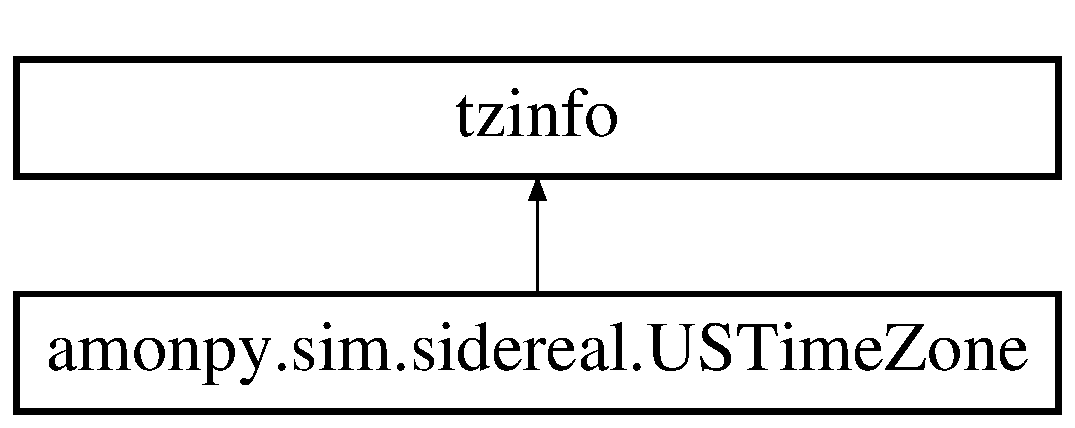
\includegraphics[height=2.000000cm]{classamonpy_1_1sim_1_1sidereal_1_1_u_s_time_zone}
\end{center}
\end{figure}
\subsection*{Public Member Functions}
\begin{DoxyCompactItemize}
\item 
def \hyperlink{classamonpy_1_1sim_1_1sidereal_1_1_u_s_time_zone_ab601802cc6ed96e739dcadd996d9587a}{\-\_\-\-\_\-init\-\_\-\-\_\-}
\item 
def \hyperlink{classamonpy_1_1sim_1_1sidereal_1_1_u_s_time_zone_a0ec12f482689f531ca39f9af8af0182c}{tzname}
\item 
def \hyperlink{classamonpy_1_1sim_1_1sidereal_1_1_u_s_time_zone_ad34a3532bf51a65d154dd7e288059ebc}{utcoffset}
\item 
def \hyperlink{classamonpy_1_1sim_1_1sidereal_1_1_u_s_time_zone_a54135cabb3cc06777a94e5912b4ff29e}{dst}
\end{DoxyCompactItemize}
\subsection*{Static Public Attributes}
\begin{DoxyCompactItemize}
\item 
tuple \hyperlink{classamonpy_1_1sim_1_1sidereal_1_1_u_s_time_zone_afea8d961d34e0b6a75bdad0f9ac41b34}{D\-S\-T\-\_\-\-S\-T\-A\-R\-T\-\_\-\-O\-L\-D} = datetime.\-datetime( 1, 4, 1, 2 )
\item 
tuple \hyperlink{classamonpy_1_1sim_1_1sidereal_1_1_u_s_time_zone_a4bb27c0cb6a5aefb11ed8c9ef9f4a5ea}{D\-S\-T\-\_\-\-E\-N\-D\-\_\-\-O\-L\-D} = datetime.\-datetime( 1, 10, 25, 2 )
\item 
tuple \hyperlink{classamonpy_1_1sim_1_1sidereal_1_1_u_s_time_zone_aa40ce77d299e1e3539f146b415383614}{D\-S\-T\-\_\-\-S\-T\-A\-R\-T\-\_\-2007} = datetime.\-datetime( 1, 3, 8, 2 )
\item 
tuple \hyperlink{classamonpy_1_1sim_1_1sidereal_1_1_u_s_time_zone_a96f5f104143b5b371c91ffbb4c01e1bd}{D\-S\-T\-\_\-\-E\-N\-D\-\_\-2007} = datetime.\-datetime( 1, 11, 1, 2 )
\end{DoxyCompactItemize}


\subsection{Detailed Description}
\begin{DoxyVerb}Represents a U.S. time zone, with automatic daylight time.

  Exports:
    USTimeZone ( hh, mm, name, stdName, dstName ):
      [ (hh is an offset east of UTC in hours) and
        (mm is an offset east of UTC in minutes) and
        (name is the composite zone name) and
        (stdName is the non-DST name) and
        (dstName is the DST name) ->
          return a new USTimeZone instance with those values ]

  State/Invariants:
    .__offset:
      [ self's offset east of UTC as a datetime.timedelta ]
    .__name:      [ as passed to constructor's name ]
    .__stdName:   [ as passed to constructor's stdName ]
    .__dstName:   [ as passed to constructor's dstName ]
\end{DoxyVerb}
 

\subsection{Constructor \& Destructor Documentation}
\hypertarget{classamonpy_1_1sim_1_1sidereal_1_1_u_s_time_zone_ab601802cc6ed96e739dcadd996d9587a}{\index{amonpy\-::sim\-::sidereal\-::\-U\-S\-Time\-Zone@{amonpy\-::sim\-::sidereal\-::\-U\-S\-Time\-Zone}!\-\_\-\-\_\-init\-\_\-\-\_\-@{\-\_\-\-\_\-init\-\_\-\-\_\-}}
\index{\-\_\-\-\_\-init\-\_\-\-\_\-@{\-\_\-\-\_\-init\-\_\-\-\_\-}!amonpy::sim::sidereal::USTimeZone@{amonpy\-::sim\-::sidereal\-::\-U\-S\-Time\-Zone}}
\subsubsection[{\-\_\-\-\_\-init\-\_\-\-\_\-}]{\setlength{\rightskip}{0pt plus 5cm}def amonpy.\-sim.\-sidereal.\-U\-S\-Time\-Zone.\-\_\-\-\_\-init\-\_\-\-\_\- (
\begin{DoxyParamCaption}
\item[{}]{self, }
\item[{}]{hh, }
\item[{}]{mm, }
\item[{}]{name, }
\item[{}]{std\-Name, }
\item[{}]{dst\-Name}
\end{DoxyParamCaption}
)}}\label{classamonpy_1_1sim_1_1sidereal_1_1_u_s_time_zone_ab601802cc6ed96e739dcadd996d9587a}


\subsection{Member Function Documentation}
\hypertarget{classamonpy_1_1sim_1_1sidereal_1_1_u_s_time_zone_a54135cabb3cc06777a94e5912b4ff29e}{\index{amonpy\-::sim\-::sidereal\-::\-U\-S\-Time\-Zone@{amonpy\-::sim\-::sidereal\-::\-U\-S\-Time\-Zone}!dst@{dst}}
\index{dst@{dst}!amonpy::sim::sidereal::USTimeZone@{amonpy\-::sim\-::sidereal\-::\-U\-S\-Time\-Zone}}
\subsubsection[{dst}]{\setlength{\rightskip}{0pt plus 5cm}def amonpy.\-sim.\-sidereal.\-U\-S\-Time\-Zone.\-dst (
\begin{DoxyParamCaption}
\item[{}]{self, }
\item[{}]{dt}
\end{DoxyParamCaption}
)}}\label{classamonpy_1_1sim_1_1sidereal_1_1_u_s_time_zone_a54135cabb3cc06777a94e5912b4ff29e}
\begin{DoxyVerb}Return the current DST offset.

  [ dt is a datetime.date ->
      if  daylight time is in effect in self's zone on
      date dt ->
return +1 hour as a datetime.timedelta
      else ->
return 0 as a datetime.delta ]
\end{DoxyVerb}
 \hypertarget{classamonpy_1_1sim_1_1sidereal_1_1_u_s_time_zone_a0ec12f482689f531ca39f9af8af0182c}{\index{amonpy\-::sim\-::sidereal\-::\-U\-S\-Time\-Zone@{amonpy\-::sim\-::sidereal\-::\-U\-S\-Time\-Zone}!tzname@{tzname}}
\index{tzname@{tzname}!amonpy::sim::sidereal::USTimeZone@{amonpy\-::sim\-::sidereal\-::\-U\-S\-Time\-Zone}}
\subsubsection[{tzname}]{\setlength{\rightskip}{0pt plus 5cm}def amonpy.\-sim.\-sidereal.\-U\-S\-Time\-Zone.\-tzname (
\begin{DoxyParamCaption}
\item[{}]{self, }
\item[{}]{dt}
\end{DoxyParamCaption}
)}}\label{classamonpy_1_1sim_1_1sidereal_1_1_u_s_time_zone_a0ec12f482689f531ca39f9af8af0182c}
\hypertarget{classamonpy_1_1sim_1_1sidereal_1_1_u_s_time_zone_ad34a3532bf51a65d154dd7e288059ebc}{\index{amonpy\-::sim\-::sidereal\-::\-U\-S\-Time\-Zone@{amonpy\-::sim\-::sidereal\-::\-U\-S\-Time\-Zone}!utcoffset@{utcoffset}}
\index{utcoffset@{utcoffset}!amonpy::sim::sidereal::USTimeZone@{amonpy\-::sim\-::sidereal\-::\-U\-S\-Time\-Zone}}
\subsubsection[{utcoffset}]{\setlength{\rightskip}{0pt plus 5cm}def amonpy.\-sim.\-sidereal.\-U\-S\-Time\-Zone.\-utcoffset (
\begin{DoxyParamCaption}
\item[{}]{self, }
\item[{}]{dt}
\end{DoxyParamCaption}
)}}\label{classamonpy_1_1sim_1_1sidereal_1_1_u_s_time_zone_ad34a3532bf51a65d154dd7e288059ebc}


\subsection{Member Data Documentation}
\hypertarget{classamonpy_1_1sim_1_1sidereal_1_1_u_s_time_zone_a96f5f104143b5b371c91ffbb4c01e1bd}{\index{amonpy\-::sim\-::sidereal\-::\-U\-S\-Time\-Zone@{amonpy\-::sim\-::sidereal\-::\-U\-S\-Time\-Zone}!D\-S\-T\-\_\-\-E\-N\-D\-\_\-2007@{D\-S\-T\-\_\-\-E\-N\-D\-\_\-2007}}
\index{D\-S\-T\-\_\-\-E\-N\-D\-\_\-2007@{D\-S\-T\-\_\-\-E\-N\-D\-\_\-2007}!amonpy::sim::sidereal::USTimeZone@{amonpy\-::sim\-::sidereal\-::\-U\-S\-Time\-Zone}}
\subsubsection[{D\-S\-T\-\_\-\-E\-N\-D\-\_\-2007}]{\setlength{\rightskip}{0pt plus 5cm}tuple amonpy.\-sim.\-sidereal.\-U\-S\-Time\-Zone.\-D\-S\-T\-\_\-\-E\-N\-D\-\_\-2007 = datetime.\-datetime( 1, 11, 1, 2 )\hspace{0.3cm}{\ttfamily [static]}}}\label{classamonpy_1_1sim_1_1sidereal_1_1_u_s_time_zone_a96f5f104143b5b371c91ffbb4c01e1bd}
\hypertarget{classamonpy_1_1sim_1_1sidereal_1_1_u_s_time_zone_a4bb27c0cb6a5aefb11ed8c9ef9f4a5ea}{\index{amonpy\-::sim\-::sidereal\-::\-U\-S\-Time\-Zone@{amonpy\-::sim\-::sidereal\-::\-U\-S\-Time\-Zone}!D\-S\-T\-\_\-\-E\-N\-D\-\_\-\-O\-L\-D@{D\-S\-T\-\_\-\-E\-N\-D\-\_\-\-O\-L\-D}}
\index{D\-S\-T\-\_\-\-E\-N\-D\-\_\-\-O\-L\-D@{D\-S\-T\-\_\-\-E\-N\-D\-\_\-\-O\-L\-D}!amonpy::sim::sidereal::USTimeZone@{amonpy\-::sim\-::sidereal\-::\-U\-S\-Time\-Zone}}
\subsubsection[{D\-S\-T\-\_\-\-E\-N\-D\-\_\-\-O\-L\-D}]{\setlength{\rightskip}{0pt plus 5cm}tuple amonpy.\-sim.\-sidereal.\-U\-S\-Time\-Zone.\-D\-S\-T\-\_\-\-E\-N\-D\-\_\-\-O\-L\-D = datetime.\-datetime( 1, 10, 25, 2 )\hspace{0.3cm}{\ttfamily [static]}}}\label{classamonpy_1_1sim_1_1sidereal_1_1_u_s_time_zone_a4bb27c0cb6a5aefb11ed8c9ef9f4a5ea}
\hypertarget{classamonpy_1_1sim_1_1sidereal_1_1_u_s_time_zone_aa40ce77d299e1e3539f146b415383614}{\index{amonpy\-::sim\-::sidereal\-::\-U\-S\-Time\-Zone@{amonpy\-::sim\-::sidereal\-::\-U\-S\-Time\-Zone}!D\-S\-T\-\_\-\-S\-T\-A\-R\-T\-\_\-2007@{D\-S\-T\-\_\-\-S\-T\-A\-R\-T\-\_\-2007}}
\index{D\-S\-T\-\_\-\-S\-T\-A\-R\-T\-\_\-2007@{D\-S\-T\-\_\-\-S\-T\-A\-R\-T\-\_\-2007}!amonpy::sim::sidereal::USTimeZone@{amonpy\-::sim\-::sidereal\-::\-U\-S\-Time\-Zone}}
\subsubsection[{D\-S\-T\-\_\-\-S\-T\-A\-R\-T\-\_\-2007}]{\setlength{\rightskip}{0pt plus 5cm}tuple amonpy.\-sim.\-sidereal.\-U\-S\-Time\-Zone.\-D\-S\-T\-\_\-\-S\-T\-A\-R\-T\-\_\-2007 = datetime.\-datetime( 1, 3, 8, 2 )\hspace{0.3cm}{\ttfamily [static]}}}\label{classamonpy_1_1sim_1_1sidereal_1_1_u_s_time_zone_aa40ce77d299e1e3539f146b415383614}
\hypertarget{classamonpy_1_1sim_1_1sidereal_1_1_u_s_time_zone_afea8d961d34e0b6a75bdad0f9ac41b34}{\index{amonpy\-::sim\-::sidereal\-::\-U\-S\-Time\-Zone@{amonpy\-::sim\-::sidereal\-::\-U\-S\-Time\-Zone}!D\-S\-T\-\_\-\-S\-T\-A\-R\-T\-\_\-\-O\-L\-D@{D\-S\-T\-\_\-\-S\-T\-A\-R\-T\-\_\-\-O\-L\-D}}
\index{D\-S\-T\-\_\-\-S\-T\-A\-R\-T\-\_\-\-O\-L\-D@{D\-S\-T\-\_\-\-S\-T\-A\-R\-T\-\_\-\-O\-L\-D}!amonpy::sim::sidereal::USTimeZone@{amonpy\-::sim\-::sidereal\-::\-U\-S\-Time\-Zone}}
\subsubsection[{D\-S\-T\-\_\-\-S\-T\-A\-R\-T\-\_\-\-O\-L\-D}]{\setlength{\rightskip}{0pt plus 5cm}tuple amonpy.\-sim.\-sidereal.\-U\-S\-Time\-Zone.\-D\-S\-T\-\_\-\-S\-T\-A\-R\-T\-\_\-\-O\-L\-D = datetime.\-datetime( 1, 4, 1, 2 )\hspace{0.3cm}{\ttfamily [static]}}}\label{classamonpy_1_1sim_1_1sidereal_1_1_u_s_time_zone_afea8d961d34e0b6a75bdad0f9ac41b34}


The documentation for this class was generated from the following file\-:\begin{DoxyCompactItemize}
\item 
amonpy/sim/\hyperlink{sidereal_8py}{sidereal.\-py}\end{DoxyCompactItemize}

\hypertarget{classamonpy_1_1sim_1_1sidereal__m_1_1_u_s_time_zone}{\section{amonpy.\-sim.\-sidereal\-\_\-m.\-U\-S\-Time\-Zone Class Reference}
\label{classamonpy_1_1sim_1_1sidereal__m_1_1_u_s_time_zone}\index{amonpy.\-sim.\-sidereal\-\_\-m.\-U\-S\-Time\-Zone@{amonpy.\-sim.\-sidereal\-\_\-m.\-U\-S\-Time\-Zone}}
}
Inheritance diagram for amonpy.\-sim.\-sidereal\-\_\-m.\-U\-S\-Time\-Zone\-:\begin{figure}[H]
\begin{center}
\leavevmode
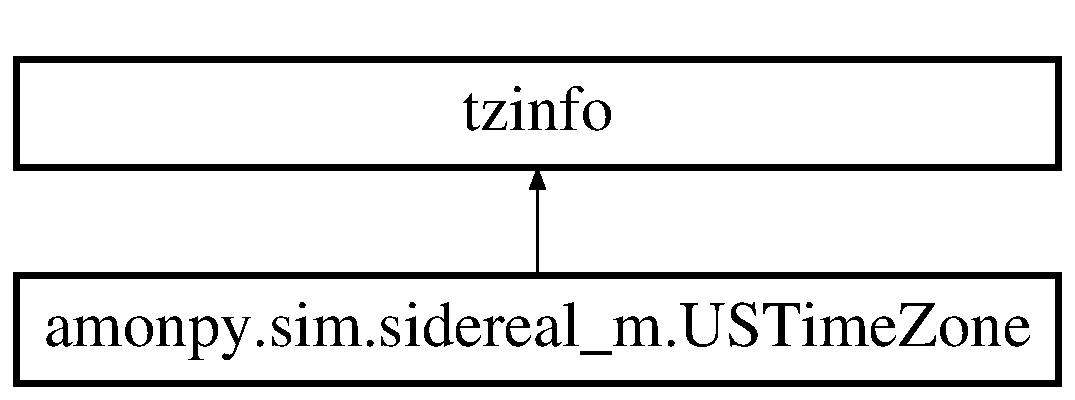
\includegraphics[height=2.000000cm]{classamonpy_1_1sim_1_1sidereal__m_1_1_u_s_time_zone}
\end{center}
\end{figure}
\subsection*{Public Member Functions}
\begin{DoxyCompactItemize}
\item 
def \hyperlink{classamonpy_1_1sim_1_1sidereal__m_1_1_u_s_time_zone_a657f7d4310310a11181f37c0dd88d836}{\-\_\-\-\_\-init\-\_\-\-\_\-}
\item 
def \hyperlink{classamonpy_1_1sim_1_1sidereal__m_1_1_u_s_time_zone_a23cff28f7e915cbedd135a6532801355}{tzname}
\item 
def \hyperlink{classamonpy_1_1sim_1_1sidereal__m_1_1_u_s_time_zone_a34b5a8e398a9fe241a92566fa1c0563b}{utcoffset}
\item 
def \hyperlink{classamonpy_1_1sim_1_1sidereal__m_1_1_u_s_time_zone_ae41bd74cd959a63c935a76f5d7f38f9c}{dst}
\end{DoxyCompactItemize}
\subsection*{Static Public Attributes}
\begin{DoxyCompactItemize}
\item 
tuple \hyperlink{classamonpy_1_1sim_1_1sidereal__m_1_1_u_s_time_zone_a6a44aff78ec6d41c874c5a47faad7bbe}{D\-S\-T\-\_\-\-S\-T\-A\-R\-T\-\_\-\-O\-L\-D} = datetime.\-datetime( 1, 4, 1, 2 )
\item 
tuple \hyperlink{classamonpy_1_1sim_1_1sidereal__m_1_1_u_s_time_zone_a6b3c892f985cb258686c386b1f2adee1}{D\-S\-T\-\_\-\-E\-N\-D\-\_\-\-O\-L\-D} = datetime.\-datetime( 1, 10, 25, 2 )
\item 
tuple \hyperlink{classamonpy_1_1sim_1_1sidereal__m_1_1_u_s_time_zone_a175d1e09720df8704393ae8c0a8c4bbd}{D\-S\-T\-\_\-\-S\-T\-A\-R\-T\-\_\-2007} = datetime.\-datetime( 1, 3, 8, 2 )
\item 
tuple \hyperlink{classamonpy_1_1sim_1_1sidereal__m_1_1_u_s_time_zone_a3aebe85ce10342323455d00f174ec2e5}{D\-S\-T\-\_\-\-E\-N\-D\-\_\-2007} = datetime.\-datetime( 1, 11, 1, 2 )
\end{DoxyCompactItemize}


\subsection{Detailed Description}
\begin{DoxyVerb}Represents a U.S. time zone, with automatic daylight time.

  Exports:
    USTimeZone ( hh, mm, name, stdName, dstName ):
      [ (hh is an offset east of UTC in hours) and
        (mm is an offset east of UTC in minutes) and
        (name is the composite zone name) and
        (stdName is the non-DST name) and
        (dstName is the DST name) ->
          return a new USTimeZone instance with those values ]

  State/Invariants:
    .__offset:
      [ self's offset east of UTC as a datetime.timedelta ]
    .__name:      [ as passed to constructor's name ]
    .__stdName:   [ as passed to constructor's stdName ]
    .__dstName:   [ as passed to constructor's dstName ]
\end{DoxyVerb}
 

\subsection{Constructor \& Destructor Documentation}
\hypertarget{classamonpy_1_1sim_1_1sidereal__m_1_1_u_s_time_zone_a657f7d4310310a11181f37c0dd88d836}{\index{amonpy\-::sim\-::sidereal\-\_\-m\-::\-U\-S\-Time\-Zone@{amonpy\-::sim\-::sidereal\-\_\-m\-::\-U\-S\-Time\-Zone}!\-\_\-\-\_\-init\-\_\-\-\_\-@{\-\_\-\-\_\-init\-\_\-\-\_\-}}
\index{\-\_\-\-\_\-init\-\_\-\-\_\-@{\-\_\-\-\_\-init\-\_\-\-\_\-}!amonpy::sim::sidereal_m::USTimeZone@{amonpy\-::sim\-::sidereal\-\_\-m\-::\-U\-S\-Time\-Zone}}
\subsubsection[{\-\_\-\-\_\-init\-\_\-\-\_\-}]{\setlength{\rightskip}{0pt plus 5cm}def amonpy.\-sim.\-sidereal\-\_\-m.\-U\-S\-Time\-Zone.\-\_\-\-\_\-init\-\_\-\-\_\- (
\begin{DoxyParamCaption}
\item[{}]{self, }
\item[{}]{hh, }
\item[{}]{mm, }
\item[{}]{name, }
\item[{}]{std\-Name, }
\item[{}]{dst\-Name}
\end{DoxyParamCaption}
)}}\label{classamonpy_1_1sim_1_1sidereal__m_1_1_u_s_time_zone_a657f7d4310310a11181f37c0dd88d836}


\subsection{Member Function Documentation}
\hypertarget{classamonpy_1_1sim_1_1sidereal__m_1_1_u_s_time_zone_ae41bd74cd959a63c935a76f5d7f38f9c}{\index{amonpy\-::sim\-::sidereal\-\_\-m\-::\-U\-S\-Time\-Zone@{amonpy\-::sim\-::sidereal\-\_\-m\-::\-U\-S\-Time\-Zone}!dst@{dst}}
\index{dst@{dst}!amonpy::sim::sidereal_m::USTimeZone@{amonpy\-::sim\-::sidereal\-\_\-m\-::\-U\-S\-Time\-Zone}}
\subsubsection[{dst}]{\setlength{\rightskip}{0pt plus 5cm}def amonpy.\-sim.\-sidereal\-\_\-m.\-U\-S\-Time\-Zone.\-dst (
\begin{DoxyParamCaption}
\item[{}]{self, }
\item[{}]{dt}
\end{DoxyParamCaption}
)}}\label{classamonpy_1_1sim_1_1sidereal__m_1_1_u_s_time_zone_ae41bd74cd959a63c935a76f5d7f38f9c}
\begin{DoxyVerb}Return the current DST offset.

  [ dt is a datetime.date ->
      if  daylight time is in effect in self's zone on
      date dt ->
return +1 hour as a datetime.timedelta
      else ->
return 0 as a datetime.delta ]
\end{DoxyVerb}
 \hypertarget{classamonpy_1_1sim_1_1sidereal__m_1_1_u_s_time_zone_a23cff28f7e915cbedd135a6532801355}{\index{amonpy\-::sim\-::sidereal\-\_\-m\-::\-U\-S\-Time\-Zone@{amonpy\-::sim\-::sidereal\-\_\-m\-::\-U\-S\-Time\-Zone}!tzname@{tzname}}
\index{tzname@{tzname}!amonpy::sim::sidereal_m::USTimeZone@{amonpy\-::sim\-::sidereal\-\_\-m\-::\-U\-S\-Time\-Zone}}
\subsubsection[{tzname}]{\setlength{\rightskip}{0pt plus 5cm}def amonpy.\-sim.\-sidereal\-\_\-m.\-U\-S\-Time\-Zone.\-tzname (
\begin{DoxyParamCaption}
\item[{}]{self, }
\item[{}]{dt}
\end{DoxyParamCaption}
)}}\label{classamonpy_1_1sim_1_1sidereal__m_1_1_u_s_time_zone_a23cff28f7e915cbedd135a6532801355}
\hypertarget{classamonpy_1_1sim_1_1sidereal__m_1_1_u_s_time_zone_a34b5a8e398a9fe241a92566fa1c0563b}{\index{amonpy\-::sim\-::sidereal\-\_\-m\-::\-U\-S\-Time\-Zone@{amonpy\-::sim\-::sidereal\-\_\-m\-::\-U\-S\-Time\-Zone}!utcoffset@{utcoffset}}
\index{utcoffset@{utcoffset}!amonpy::sim::sidereal_m::USTimeZone@{amonpy\-::sim\-::sidereal\-\_\-m\-::\-U\-S\-Time\-Zone}}
\subsubsection[{utcoffset}]{\setlength{\rightskip}{0pt plus 5cm}def amonpy.\-sim.\-sidereal\-\_\-m.\-U\-S\-Time\-Zone.\-utcoffset (
\begin{DoxyParamCaption}
\item[{}]{self, }
\item[{}]{dt}
\end{DoxyParamCaption}
)}}\label{classamonpy_1_1sim_1_1sidereal__m_1_1_u_s_time_zone_a34b5a8e398a9fe241a92566fa1c0563b}


\subsection{Member Data Documentation}
\hypertarget{classamonpy_1_1sim_1_1sidereal__m_1_1_u_s_time_zone_a3aebe85ce10342323455d00f174ec2e5}{\index{amonpy\-::sim\-::sidereal\-\_\-m\-::\-U\-S\-Time\-Zone@{amonpy\-::sim\-::sidereal\-\_\-m\-::\-U\-S\-Time\-Zone}!D\-S\-T\-\_\-\-E\-N\-D\-\_\-2007@{D\-S\-T\-\_\-\-E\-N\-D\-\_\-2007}}
\index{D\-S\-T\-\_\-\-E\-N\-D\-\_\-2007@{D\-S\-T\-\_\-\-E\-N\-D\-\_\-2007}!amonpy::sim::sidereal_m::USTimeZone@{amonpy\-::sim\-::sidereal\-\_\-m\-::\-U\-S\-Time\-Zone}}
\subsubsection[{D\-S\-T\-\_\-\-E\-N\-D\-\_\-2007}]{\setlength{\rightskip}{0pt plus 5cm}tuple amonpy.\-sim.\-sidereal\-\_\-m.\-U\-S\-Time\-Zone.\-D\-S\-T\-\_\-\-E\-N\-D\-\_\-2007 = datetime.\-datetime( 1, 11, 1, 2 )\hspace{0.3cm}{\ttfamily [static]}}}\label{classamonpy_1_1sim_1_1sidereal__m_1_1_u_s_time_zone_a3aebe85ce10342323455d00f174ec2e5}
\hypertarget{classamonpy_1_1sim_1_1sidereal__m_1_1_u_s_time_zone_a6b3c892f985cb258686c386b1f2adee1}{\index{amonpy\-::sim\-::sidereal\-\_\-m\-::\-U\-S\-Time\-Zone@{amonpy\-::sim\-::sidereal\-\_\-m\-::\-U\-S\-Time\-Zone}!D\-S\-T\-\_\-\-E\-N\-D\-\_\-\-O\-L\-D@{D\-S\-T\-\_\-\-E\-N\-D\-\_\-\-O\-L\-D}}
\index{D\-S\-T\-\_\-\-E\-N\-D\-\_\-\-O\-L\-D@{D\-S\-T\-\_\-\-E\-N\-D\-\_\-\-O\-L\-D}!amonpy::sim::sidereal_m::USTimeZone@{amonpy\-::sim\-::sidereal\-\_\-m\-::\-U\-S\-Time\-Zone}}
\subsubsection[{D\-S\-T\-\_\-\-E\-N\-D\-\_\-\-O\-L\-D}]{\setlength{\rightskip}{0pt plus 5cm}tuple amonpy.\-sim.\-sidereal\-\_\-m.\-U\-S\-Time\-Zone.\-D\-S\-T\-\_\-\-E\-N\-D\-\_\-\-O\-L\-D = datetime.\-datetime( 1, 10, 25, 2 )\hspace{0.3cm}{\ttfamily [static]}}}\label{classamonpy_1_1sim_1_1sidereal__m_1_1_u_s_time_zone_a6b3c892f985cb258686c386b1f2adee1}
\hypertarget{classamonpy_1_1sim_1_1sidereal__m_1_1_u_s_time_zone_a175d1e09720df8704393ae8c0a8c4bbd}{\index{amonpy\-::sim\-::sidereal\-\_\-m\-::\-U\-S\-Time\-Zone@{amonpy\-::sim\-::sidereal\-\_\-m\-::\-U\-S\-Time\-Zone}!D\-S\-T\-\_\-\-S\-T\-A\-R\-T\-\_\-2007@{D\-S\-T\-\_\-\-S\-T\-A\-R\-T\-\_\-2007}}
\index{D\-S\-T\-\_\-\-S\-T\-A\-R\-T\-\_\-2007@{D\-S\-T\-\_\-\-S\-T\-A\-R\-T\-\_\-2007}!amonpy::sim::sidereal_m::USTimeZone@{amonpy\-::sim\-::sidereal\-\_\-m\-::\-U\-S\-Time\-Zone}}
\subsubsection[{D\-S\-T\-\_\-\-S\-T\-A\-R\-T\-\_\-2007}]{\setlength{\rightskip}{0pt plus 5cm}tuple amonpy.\-sim.\-sidereal\-\_\-m.\-U\-S\-Time\-Zone.\-D\-S\-T\-\_\-\-S\-T\-A\-R\-T\-\_\-2007 = datetime.\-datetime( 1, 3, 8, 2 )\hspace{0.3cm}{\ttfamily [static]}}}\label{classamonpy_1_1sim_1_1sidereal__m_1_1_u_s_time_zone_a175d1e09720df8704393ae8c0a8c4bbd}
\hypertarget{classamonpy_1_1sim_1_1sidereal__m_1_1_u_s_time_zone_a6a44aff78ec6d41c874c5a47faad7bbe}{\index{amonpy\-::sim\-::sidereal\-\_\-m\-::\-U\-S\-Time\-Zone@{amonpy\-::sim\-::sidereal\-\_\-m\-::\-U\-S\-Time\-Zone}!D\-S\-T\-\_\-\-S\-T\-A\-R\-T\-\_\-\-O\-L\-D@{D\-S\-T\-\_\-\-S\-T\-A\-R\-T\-\_\-\-O\-L\-D}}
\index{D\-S\-T\-\_\-\-S\-T\-A\-R\-T\-\_\-\-O\-L\-D@{D\-S\-T\-\_\-\-S\-T\-A\-R\-T\-\_\-\-O\-L\-D}!amonpy::sim::sidereal_m::USTimeZone@{amonpy\-::sim\-::sidereal\-\_\-m\-::\-U\-S\-Time\-Zone}}
\subsubsection[{D\-S\-T\-\_\-\-S\-T\-A\-R\-T\-\_\-\-O\-L\-D}]{\setlength{\rightskip}{0pt plus 5cm}tuple amonpy.\-sim.\-sidereal\-\_\-m.\-U\-S\-Time\-Zone.\-D\-S\-T\-\_\-\-S\-T\-A\-R\-T\-\_\-\-O\-L\-D = datetime.\-datetime( 1, 4, 1, 2 )\hspace{0.3cm}{\ttfamily [static]}}}\label{classamonpy_1_1sim_1_1sidereal__m_1_1_u_s_time_zone_a6a44aff78ec6d41c874c5a47faad7bbe}


The documentation for this class was generated from the following file\-:\begin{DoxyCompactItemize}
\item 
amonpy/sim/\hyperlink{sidereal__m_8py}{sidereal\-\_\-m.\-py}\end{DoxyCompactItemize}

\chapter{File Documentation}
\hypertarget{____init_____8py}{\section{amonpy/\-\_\-\-\_\-init\-\_\-\-\_\-.py File Reference}
\label{____init_____8py}\index{amonpy/\-\_\-\-\_\-init\-\_\-\-\_\-.\-py@{amonpy/\-\_\-\-\_\-init\-\_\-\-\_\-.\-py}}
}
\subsection*{Namespaces}
\begin{DoxyCompactItemize}
\item 
\hyperlink{namespaceamonpy}{amonpy}
\end{DoxyCompactItemize}
\subsection*{Constant Groups}
\begin{DoxyCompactItemize}
\item 
\hyperlink{namespaceamonpy}{amonpy}
\end{DoxyCompactItemize}

\hypertarget{anal_2____init_____8py}{\section{amonpy/anal/\-\_\-\-\_\-init\-\_\-\-\_\-.py File Reference}
\label{anal_2____init_____8py}\index{amonpy/anal/\-\_\-\-\_\-init\-\_\-\-\_\-.\-py@{amonpy/anal/\-\_\-\-\_\-init\-\_\-\-\_\-.\-py}}
}
\subsection*{Namespaces}
\begin{DoxyCompactItemize}
\item 
\hyperlink{namespaceamonpy_1_1anal}{amonpy.\-anal}
\end{DoxyCompactItemize}
\subsection*{Constant Groups}
\begin{DoxyCompactItemize}
\item 
\hyperlink{namespaceamonpy_1_1anal}{amonpy.\-anal}
\end{DoxyCompactItemize}

\hypertarget{dbase_2____init_____8py}{\section{amonpy/dbase/\-\_\-\-\_\-init\-\_\-\-\_\-.py File Reference}
\label{dbase_2____init_____8py}\index{amonpy/dbase/\-\_\-\-\_\-init\-\_\-\-\_\-.\-py@{amonpy/dbase/\-\_\-\-\_\-init\-\_\-\-\_\-.\-py}}
}
\subsection*{Namespaces}
\begin{DoxyCompactItemize}
\item 
\hyperlink{namespaceamonpy_1_1dbase}{amonpy.\-dbase}
\end{DoxyCompactItemize}
\subsection*{Constant Groups}
\begin{DoxyCompactItemize}
\item 
\hyperlink{namespaceamonpy_1_1dbase}{amonpy.\-dbase}
\end{DoxyCompactItemize}

\hypertarget{dbase_2test_2____init_____8py}{\section{amonpy/dbase/test/\-\_\-\-\_\-init\-\_\-\-\_\-.py File Reference}
\label{dbase_2test_2____init_____8py}\index{amonpy/dbase/test/\-\_\-\-\_\-init\-\_\-\-\_\-.\-py@{amonpy/dbase/test/\-\_\-\-\_\-init\-\_\-\-\_\-.\-py}}
}
\subsection*{Namespaces}
\begin{DoxyCompactItemize}
\item 
\hyperlink{namespaceamonpy_1_1dbase_1_1test}{amonpy.\-dbase.\-test}
\end{DoxyCompactItemize}
\subsection*{Constant Groups}
\begin{DoxyCompactItemize}
\item 
\hyperlink{namespaceamonpy_1_1dbase_1_1test}{amonpy.\-dbase.\-test}
\end{DoxyCompactItemize}

\hypertarget{sim_2____init_____8py}{\section{amonpy/sim/\-\_\-\-\_\-init\-\_\-\-\_\-.py File Reference}
\label{sim_2____init_____8py}\index{amonpy/sim/\-\_\-\-\_\-init\-\_\-\-\_\-.\-py@{amonpy/sim/\-\_\-\-\_\-init\-\_\-\-\_\-.\-py}}
}
\subsection*{Namespaces}
\begin{DoxyCompactItemize}
\item 
\hyperlink{namespaceamonpy_1_1sim}{amonpy.\-sim}
\end{DoxyCompactItemize}
\subsection*{Constant Groups}
\begin{DoxyCompactItemize}
\item 
\hyperlink{namespaceamonpy_1_1sim}{amonpy.\-sim}
\end{DoxyCompactItemize}
\subsection*{Variables}
\begin{DoxyCompactItemize}
\item 
list \hyperlink{namespaceamonpy_1_1sim_a88c074ad5a5920622371de9472a7290b}{amonpy.\-sim.\-\_\-\-\_\-all\-\_\-\-\_\-} = \mbox{[}\char`\"{}basic\-\_\-sim\char`\"{}, \char`\"{}sidereal\char`\"{}, \char`\"{}sidereal\-\_\-m\char`\"{}\mbox{]}
\end{DoxyCompactItemize}

\hypertarget{tools_2____init_____8py}{\section{amonpy/tools/\-\_\-\-\_\-init\-\_\-\-\_\-.py File Reference}
\label{tools_2____init_____8py}\index{amonpy/tools/\-\_\-\-\_\-init\-\_\-\-\_\-.\-py@{amonpy/tools/\-\_\-\-\_\-init\-\_\-\-\_\-.\-py}}
}
\subsection*{Namespaces}
\begin{DoxyCompactItemize}
\item 
\hyperlink{namespaceamonpy_1_1tools}{amonpy.\-tools}
\end{DoxyCompactItemize}
\subsection*{Constant Groups}
\begin{DoxyCompactItemize}
\item 
\hyperlink{namespaceamonpy_1_1tools}{amonpy.\-tools}
\end{DoxyCompactItemize}

\hypertarget{analysis_8py}{\section{amonpy/anal/analysis.py File Reference}
\label{analysis_8py}\index{amonpy/anal/analysis.\-py@{amonpy/anal/analysis.\-py}}
}
\subsection*{Namespaces}
\begin{DoxyCompactItemize}
\item 
\hyperlink{namespaceamonpy_1_1anal_1_1analysis}{amonpy.\-anal.\-analysis}
\end{DoxyCompactItemize}
\subsection*{Constant Groups}
\begin{DoxyCompactItemize}
\item 
\hyperlink{namespaceamonpy_1_1anal_1_1analysis}{amonpy.\-anal.\-analysis}
\end{DoxyCompactItemize}

\hypertarget{cluster_8py}{\section{amonpy/anal/cluster.py File Reference}
\label{cluster_8py}\index{amonpy/anal/cluster.\-py@{amonpy/anal/cluster.\-py}}
}
\subsection*{Classes}
\begin{DoxyCompactItemize}
\item 
class \hyperlink{classamonpy_1_1anal_1_1cluster_1_1_fisher__doublet}{amonpy.\-anal.\-cluster.\-Fisher\-\_\-doublet}
\begin{DoxyCompactList}\small\item\em Analysis class object that uses the \hyperlink{classamonpy_1_1anal_1_1cluster_1_1_fisher}{Fisher} P\-S\-F In particular, the \hyperlink{classamonpy_1_1anal_1_1cluster_1_1_fisher}{Fisher} P\-S\-F is axially symmetric with a single parameter sigma. \end{DoxyCompactList}\item 
class \hyperlink{classamonpy_1_1anal_1_1cluster_1_1_fisher__tp}{amonpy.\-anal.\-cluster.\-Fisher\-\_\-tp}
\begin{DoxyCompactList}\small\item\em Analysis class object that uses the \hyperlink{classamonpy_1_1anal_1_1cluster_1_1_fisher}{Fisher} P\-S\-F In particular, the \hyperlink{classamonpy_1_1anal_1_1cluster_1_1_fisher}{Fisher} P\-S\-F is axially symmetric with a single parameter sigma. \end{DoxyCompactList}\item 
class \hyperlink{classamonpy_1_1anal_1_1cluster_1_1_fisher}{amonpy.\-anal.\-cluster.\-Fisher}
\begin{DoxyCompactList}\small\item\em Analysis class object that uses the \hyperlink{classamonpy_1_1anal_1_1cluster_1_1_fisher}{Fisher} P\-S\-F In particular, the \hyperlink{classamonpy_1_1anal_1_1cluster_1_1_fisher}{Fisher} P\-S\-F is axially symmetric with a single parameter sigma. \end{DoxyCompactList}\end{DoxyCompactItemize}
\subsection*{Namespaces}
\begin{DoxyCompactItemize}
\item 
\hyperlink{namespaceamonpy_1_1anal_1_1cluster}{amonpy.\-anal.\-cluster}
\item 
\hyperlink{namespacecluster}{cluster}
\begin{DoxyCompactList}\small\item\em Module defining analysis class objects for clustering. \end{DoxyCompactList}\end{DoxyCompactItemize}
\subsection*{Constant Groups}
\begin{DoxyCompactItemize}
\item 
\hyperlink{namespaceamonpy_1_1anal_1_1cluster}{amonpy.\-anal.\-cluster}
\item 
\hyperlink{namespacecluster}{cluster}
\begin{DoxyCompactList}\small\item\em Module defining analysis class objects for clustering. \end{DoxyCompactList}\end{DoxyCompactItemize}

\hypertarget{pvalue__form_8py}{\section{amonpy/anal/pvalue\-\_\-form.py File Reference}
\label{pvalue__form_8py}\index{amonpy/anal/pvalue\-\_\-form.\-py@{amonpy/anal/pvalue\-\_\-form.\-py}}
}
\subsection*{Namespaces}
\begin{DoxyCompactItemize}
\item 
\hyperlink{namespaceamonpy_1_1anal_1_1pvalue__form}{amonpy.\-anal.\-pvalue\-\_\-form}
\item 
\hyperlink{namespacepvalue__form}{pvalue\-\_\-form}
\begin{DoxyCompactList}\small\item\em \begin{DoxyVerb}Package that combines p-values from different streams using different methods.\end{DoxyVerb}
 \end{DoxyCompactList}\end{DoxyCompactItemize}
\subsection*{Constant Groups}
\begin{DoxyCompactItemize}
\item 
\hyperlink{namespaceamonpy_1_1anal_1_1pvalue__form}{amonpy.\-anal.\-pvalue\-\_\-form}
\item 
\hyperlink{namespacepvalue__form}{pvalue\-\_\-form}
\begin{DoxyCompactList}\small\item\em \begin{DoxyVerb}Package that combines p-values from different streams using different methods.\end{DoxyVerb}
 \end{DoxyCompactList}\end{DoxyCompactItemize}
\subsection*{Functions}
\begin{DoxyCompactItemize}
\item 
def \hyperlink{namespaceamonpy_1_1anal_1_1pvalue__form_a828ea7843c6366d3897e6172c104de6a}{amonpy.\-anal.\-pvalue\-\_\-form.\-check\-\_\-pvalues}
\item 
def \hyperlink{namespaceamonpy_1_1anal_1_1pvalue__form_a670904b2f9cf749a5a19110bd02f271d}{amonpy.\-anal.\-pvalue\-\_\-form.\-pvalue\-\_\-fisher}
\begin{DoxyCompactList}\small\item\em Combining p-\/values using Fisher method. \end{DoxyCompactList}\item 
def \hyperlink{namespaceamonpy_1_1anal_1_1pvalue__form_aa18a5556dd27f37b93797598d69ea369}{amonpy.\-anal.\-pvalue\-\_\-form.\-pvalue\-\_\-fisher\-\_\-log}
\begin{DoxyCompactList}\small\item\em Combining p-\/values using Fisher method. \end{DoxyCompactList}\item 
def \hyperlink{namespaceamonpy_1_1anal_1_1pvalue__form_a668ad1e4b4f4340f31887de63f5ad752}{amonpy.\-anal.\-pvalue\-\_\-form.\-pvalue\-\_\-good}
\begin{DoxyCompactList}\small\item\em Combines p-\/values using Good's formula References\-: Ar\-Xiv e-\/print 1011.\-6627, 2010. \end{DoxyCompactList}\item 
def \hyperlink{namespaceamonpy_1_1anal_1_1pvalue__form_aa109ec563316742673820874876406a0}{amonpy.\-anal.\-pvalue\-\_\-form.\-pvalue\-\_\-good\-\_\-log}
\begin{DoxyCompactList}\small\item\em Combines p-\/values using Good's formula. \end{DoxyCompactList}\item 
def \hyperlink{namespaceamonpy_1_1anal_1_1pvalue__form_aae316cb4d8782c8cbdb9564fb3d293c9}{amonpy.\-anal.\-pvalue\-\_\-form.\-good\-\_\-denominator}
\begin{DoxyCompactList}\small\item\em Denominator in Goods formula (product of weight differences) \end{DoxyCompactList}\end{DoxyCompactItemize}

\hypertarget{test__analysis_8py}{\section{amonpy/anal/test/test\-\_\-analysis.py File Reference}
\label{test__analysis_8py}\index{amonpy/anal/test/test\-\_\-analysis.\-py@{amonpy/anal/test/test\-\_\-analysis.\-py}}
}
\subsection*{Namespaces}
\begin{DoxyCompactItemize}
\item 
\hyperlink{namespacetest__analysis}{test\-\_\-analysis}
\end{DoxyCompactItemize}
\subsection*{Constant Groups}
\begin{DoxyCompactItemize}
\item 
\hyperlink{namespacetest__analysis}{test\-\_\-analysis}
\end{DoxyCompactItemize}

\hypertarget{add__stream_8py}{\section{amonpy/dbase/add\-\_\-stream.py File Reference}
\label{add__stream_8py}\index{amonpy/dbase/add\-\_\-stream.\-py@{amonpy/dbase/add\-\_\-stream.\-py}}
}
\subsection*{Namespaces}
\begin{DoxyCompactItemize}
\item 
\hyperlink{namespaceamonpy_1_1dbase_1_1add__stream}{amonpy.\-dbase.\-add\-\_\-stream}
\end{DoxyCompactItemize}
\subsection*{Constant Groups}
\begin{DoxyCompactItemize}
\item 
\hyperlink{namespaceamonpy_1_1dbase_1_1add__stream}{amonpy.\-dbase.\-add\-\_\-stream}
\end{DoxyCompactItemize}

\hypertarget{add__user_8py}{\section{amonpy/dbase/add\-\_\-user.py File Reference}
\label{add__user_8py}\index{amonpy/dbase/add\-\_\-user.\-py@{amonpy/dbase/add\-\_\-user.\-py}}
}
\subsection*{Namespaces}
\begin{DoxyCompactItemize}
\item 
\hyperlink{namespaceamonpy_1_1dbase_1_1add__user}{amonpy.\-dbase.\-add\-\_\-user}
\end{DoxyCompactItemize}
\subsection*{Constant Groups}
\begin{DoxyCompactItemize}
\item 
\hyperlink{namespaceamonpy_1_1dbase_1_1add__user}{amonpy.\-dbase.\-add\-\_\-user}
\end{DoxyCompactItemize}

\hypertarget{dbase_2alert__to__voevent_8py}{\section{amonpy/dbase/alert\-\_\-to\-\_\-voevent.py File Reference}
\label{dbase_2alert__to__voevent_8py}\index{amonpy/dbase/alert\-\_\-to\-\_\-voevent.\-py@{amonpy/dbase/alert\-\_\-to\-\_\-voevent.\-py}}
}
\subsection*{Namespaces}
\begin{DoxyCompactItemize}
\item 
\hyperlink{namespaceamonpy_1_1dbase_1_1alert__to__voevent}{amonpy.\-dbase.\-alert\-\_\-to\-\_\-voevent}
\end{DoxyCompactItemize}
\subsection*{Constant Groups}
\begin{DoxyCompactItemize}
\item 
\hyperlink{namespaceamonpy_1_1dbase_1_1alert__to__voevent}{amonpy.\-dbase.\-alert\-\_\-to\-\_\-voevent}
\end{DoxyCompactItemize}

\hypertarget{dev_2alert__to__voevent_8py}{\section{amonpy/dev/alert\-\_\-to\-\_\-voevent.py File Reference}
\label{dev_2alert__to__voevent_8py}\index{amonpy/dev/alert\-\_\-to\-\_\-voevent.\-py@{amonpy/dev/alert\-\_\-to\-\_\-voevent.\-py}}
}
\subsection*{Namespaces}
\begin{DoxyCompactItemize}
\item 
\hyperlink{namespacealert__to__voevent}{alert\-\_\-to\-\_\-voevent}
\end{DoxyCompactItemize}
\subsection*{Constant Groups}
\begin{DoxyCompactItemize}
\item 
\hyperlink{namespacealert__to__voevent}{alert\-\_\-to\-\_\-voevent}
\end{DoxyCompactItemize}
\subsection*{Functions}
\begin{DoxyCompactItemize}
\item 
def \hyperlink{namespacealert__to__voevent_af5936ba55fd75b4f07770c759a71f8a5}{alert\-\_\-to\-\_\-voevent.\-alert\-\_\-to\-\_\-voevent}
\end{DoxyCompactItemize}
\subsection*{Variables}
\begin{DoxyCompactItemize}
\item 
list \hyperlink{namespacealert__to__voevent_a4f4d8458b2c52fe0aa899e49fe69f9db}{alert\-\_\-to\-\_\-voevent.\-alert} = \mbox{[}Alert(1,0,0)\mbox{]}
\item 
tuple \hyperlink{namespacealert__to__voevent_ac245971d0da32191244c1bff1550382c}{alert\-\_\-to\-\_\-voevent.\-xml1} = alert\-\_\-to\-\_\-voevent(\hyperlink{db__mc__build_8sql_a38a604686c7d372f50752e893e3e1e21}{alert})
\item 
tuple \hyperlink{namespacealert__to__voevent_ad16a5fe14209236bf0dec996bd4d8031}{alert\-\_\-to\-\_\-voevent.\-f1} = open('./test\-\_\-alert.\-xml', 'w+')
\end{DoxyCompactItemize}

\hypertarget{archive_8py}{\section{amonpy/dbase/archive.py File Reference}
\label{archive_8py}\index{amonpy/dbase/archive.\-py@{amonpy/dbase/archive.\-py}}
}
\subsection*{Namespaces}
\begin{DoxyCompactItemize}
\item 
\hyperlink{namespaceamonpy_1_1dbase_1_1archive}{amonpy.\-dbase.\-archive}
\end{DoxyCompactItemize}
\subsection*{Constant Groups}
\begin{DoxyCompactItemize}
\item 
\hyperlink{namespaceamonpy_1_1dbase_1_1archive}{amonpy.\-dbase.\-archive}
\end{DoxyCompactItemize}

\hypertarget{config__alert__stream_8py}{\section{amonpy/dbase/config\-\_\-alert\-\_\-stream.py File Reference}
\label{config__alert__stream_8py}\index{amonpy/dbase/config\-\_\-alert\-\_\-stream.\-py@{amonpy/dbase/config\-\_\-alert\-\_\-stream.\-py}}
}
\subsection*{Namespaces}
\begin{DoxyCompactItemize}
\item 
\hyperlink{namespaceamonpy_1_1dbase_1_1config__alert__stream}{amonpy.\-dbase.\-config\-\_\-alert\-\_\-stream}
\end{DoxyCompactItemize}
\subsection*{Constant Groups}
\begin{DoxyCompactItemize}
\item 
\hyperlink{namespaceamonpy_1_1dbase_1_1config__alert__stream}{amonpy.\-dbase.\-config\-\_\-alert\-\_\-stream}
\end{DoxyCompactItemize}

\hypertarget{config__event__stream_8py}{\section{amonpy/dbase/config\-\_\-event\-\_\-stream.py File Reference}
\label{config__event__stream_8py}\index{amonpy/dbase/config\-\_\-event\-\_\-stream.\-py@{amonpy/dbase/config\-\_\-event\-\_\-stream.\-py}}
}
\subsection*{Namespaces}
\begin{DoxyCompactItemize}
\item 
\hyperlink{namespaceamonpy_1_1dbase_1_1config__event__stream}{amonpy.\-dbase.\-config\-\_\-event\-\_\-stream}
\end{DoxyCompactItemize}
\subsection*{Constant Groups}
\begin{DoxyCompactItemize}
\item 
\hyperlink{namespaceamonpy_1_1dbase_1_1config__event__stream}{amonpy.\-dbase.\-config\-\_\-event\-\_\-stream}
\end{DoxyCompactItemize}

\hypertarget{db__classes_8py}{\section{amonpy/dbase/db\-\_\-classes.py File Reference}
\label{db__classes_8py}\index{amonpy/dbase/db\-\_\-classes.\-py@{amonpy/dbase/db\-\_\-classes.\-py}}
}
\subsection*{Classes}
\begin{DoxyCompactItemize}
\item 
class \hyperlink{classamonpy_1_1dbase_1_1db__classes_1_1_alert}{amonpy.\-dbase.\-db\-\_\-classes.\-Alert}
\begin{DoxyCompactList}\small\item\em Creates the \hyperlink{classamonpy_1_1dbase_1_1db__classes_1_1_alert}{Alert} class. \end{DoxyCompactList}\item 
class \hyperlink{classamonpy_1_1dbase_1_1db__classes_1_1_event_stream_config}{amonpy.\-dbase.\-db\-\_\-classes.\-Event\-Stream\-Config}
\begin{DoxyCompactList}\small\item\em Creates the \hyperlink{classamonpy_1_1dbase_1_1db__classes_1_1_event_stream_config}{Event\-Stream\-Config} class. \end{DoxyCompactList}\item 
class \hyperlink{classamonpy_1_1dbase_1_1db__classes_1_1_alert_config}{amonpy.\-dbase.\-db\-\_\-classes.\-Alert\-Config}
\begin{DoxyCompactList}\small\item\em Creates the \hyperlink{classamonpy_1_1dbase_1_1db__classes_1_1_alert_config}{Alert\-Config} class. \end{DoxyCompactList}\item 
class \hyperlink{classamonpy_1_1dbase_1_1db__classes_1_1_alert_config2}{amonpy.\-dbase.\-db\-\_\-classes.\-Alert\-Config2}
\begin{DoxyCompactList}\small\item\em Creates the \hyperlink{classamonpy_1_1dbase_1_1db__classes_1_1_alert_config2}{Alert\-Config2} test class. \end{DoxyCompactList}\item 
class \hyperlink{classamonpy_1_1dbase_1_1db__classes_1_1_alert_line}{amonpy.\-dbase.\-db\-\_\-classes.\-Alert\-Line}
\begin{DoxyCompactList}\small\item\em Creates the \hyperlink{classamonpy_1_1dbase_1_1db__classes_1_1_alert_line}{Alert\-Line} class. \end{DoxyCompactList}\item 
class \hyperlink{classamonpy_1_1dbase_1_1db__classes_1_1_parameter}{amonpy.\-dbase.\-db\-\_\-classes.\-Parameter}
\begin{DoxyCompactList}\small\item\em Creates the \hyperlink{classamonpy_1_1dbase_1_1db__classes_1_1_parameter}{Parameter} class. \end{DoxyCompactList}\end{DoxyCompactItemize}
\subsection*{Namespaces}
\begin{DoxyCompactItemize}
\item 
\hyperlink{namespaceamonpy_1_1dbase_1_1db__classes}{amonpy.\-dbase.\-db\-\_\-classes}
\item 
\hyperlink{namespacedb__classes}{db\-\_\-classes}
\begin{DoxyCompactList}\small\item\em Builds the basic classes (Event, Alert, etc), that correspond to tables in the A\-M\-O\-N database. \end{DoxyCompactList}\end{DoxyCompactItemize}
\subsection*{Constant Groups}
\begin{DoxyCompactItemize}
\item 
\hyperlink{namespaceamonpy_1_1dbase_1_1db__classes}{amonpy.\-dbase.\-db\-\_\-classes}
\item 
\hyperlink{namespacedb__classes}{db\-\_\-classes}
\begin{DoxyCompactList}\small\item\em Builds the basic classes (Event, Alert, etc), that correspond to tables in the A\-M\-O\-N database. \end{DoxyCompactList}\end{DoxyCompactItemize}
\subsection*{Functions}
\begin{DoxyCompactItemize}
\item 
def \hyperlink{namespaceamonpy_1_1dbase_1_1db__classes_a17d82764a82f5d4057aa427d04a745cd}{amonpy.\-dbase.\-db\-\_\-classes.\-wherewhen\-\_\-def}
\begin{DoxyCompactList}\small\item\em wherewhen\-\_\-def is a class factory function Optional Inputs\-: args\mbox{[}0\mbox{]} is an object from the \hyperlink{classamonpy_1_1dbase_1_1db__classes_1_1_event_stream_config}{Event\-Stream\-Config} class args\mbox{[}1\mbox{]} set to True if simulation is desired Output\-: returns the Where\-When class \end{DoxyCompactList}\item 
def \hyperlink{namespaceamonpy_1_1dbase_1_1db__classes_a6d7088f9593d82867532ef736e26f2f7}{amonpy.\-dbase.\-db\-\_\-classes.\-event\-\_\-def}
\begin{DoxyCompactList}\small\item\em event\-\_\-def is a class factory function Optional Inputs\-: args\mbox{[}0\mbox{]} is an object from the \hyperlink{classamonpy_1_1dbase_1_1db__classes_1_1_event_stream_config}{Event\-Stream\-Config} class args\mbox{[}1\mbox{]} set to True if simulaiton is desired Output\-: returns the Event class \end{DoxyCompactList}\item 
def \hyperlink{namespaceamonpy_1_1dbase_1_1db__classes_a5ac6184a9ebdc45d52f961dd4e2ae1fd}{amonpy.\-dbase.\-db\-\_\-classes.\-simstream}
\begin{DoxyCompactList}\small\item\em Some examples of the \hyperlink{classamonpy_1_1dbase_1_1db__classes_1_1_event_stream_config}{Event\-Stream\-Config} class which are used to demonstrate simulations for Amon\-Py v0.\-1. \end{DoxyCompactList}\item 
def \hyperlink{namespaceamonpy_1_1dbase_1_1db__classes_a06a8874ab6b9b555ec11356861fb94a2}{amonpy.\-dbase.\-db\-\_\-classes.\-ex\-Alert\-Config}
\begin{DoxyCompactList}\small\item\em Returns an example \hyperlink{classamonpy_1_1dbase_1_1db__classes_1_1_alert_config}{Alert\-Config} object, used for testing the analysis code. \end{DoxyCompactList}\item 
def \hyperlink{namespaceamonpy_1_1dbase_1_1db__classes_a67783ae65776e6bb779b928405b44879}{amonpy.\-dbase.\-db\-\_\-classes.\-ex\-Alert\-Archiv\-Config}
\begin{DoxyCompactList}\small\item\em Returns an example \hyperlink{classamonpy_1_1dbase_1_1db__classes_1_1_alert_config}{Alert\-Config} object, used for testing the analysis code. \end{DoxyCompactList}\end{DoxyCompactItemize}
\subsection*{Variables}
\begin{DoxyCompactItemize}
\item 
tuple \hyperlink{namespaceamonpy_1_1dbase_1_1db__classes_addf9b6ab76d93bfdebf988a2895ff34f}{amonpy.\-dbase.\-db\-\_\-classes.\-Event} = event\-\_\-def()
\item 
\hyperlink{namespaceamonpy_1_1dbase_1_1db__classes_ae05fd637497daebdcb0cca7044926cd3}{amonpy.\-dbase.\-db\-\_\-classes.\-sigma\-R}
\item 
\hyperlink{namespaceamonpy_1_1dbase_1_1db__classes_ad0767f5c0c80ad02abbf61aab485b444}{amonpy.\-dbase.\-db\-\_\-classes.\-sigma\-T}
\item 
\hyperlink{namespaceamonpy_1_1dbase_1_1db__classes_abffb2aca4c4fae167e7d385c22f528b3}{amonpy.\-dbase.\-db\-\_\-classes.\-point\-\_\-\-R\-A}
\item 
\hyperlink{namespaceamonpy_1_1dbase_1_1db__classes_a6c4dfc506de762cbb50a8cdebc263e8e}{amonpy.\-dbase.\-db\-\_\-classes.\-point\-\_\-dec}
\item 
\hyperlink{namespaceamonpy_1_1dbase_1_1db__classes_a15a38b01ffc48ef3ca06d3378afaedcd}{amonpy.\-dbase.\-db\-\_\-classes.\-longitude}
\item 
\hyperlink{namespaceamonpy_1_1dbase_1_1db__classes_a5b23674f16dd7136e87b30c0f7cb2194}{amonpy.\-dbase.\-db\-\_\-classes.\-latitude}
\item 
\hyperlink{namespaceamonpy_1_1dbase_1_1db__classes_a5a1632bf843d0f0ae5900eb04aaad787}{amonpy.\-dbase.\-db\-\_\-classes.\-elevation}
\item 
\hyperlink{namespaceamonpy_1_1dbase_1_1db__classes_ae78b921654586e117c92fec127c99be1}{amonpy.\-dbase.\-db\-\_\-classes.\-datetime}
\item 
\hyperlink{namespaceamonpy_1_1dbase_1_1db__classes_ace7891a3d914ddc3aada697fc748e7b7}{amonpy.\-dbase.\-db\-\_\-classes.\-R\-A}
\item 
\hyperlink{namespaceamonpy_1_1dbase_1_1db__classes_ae45e4ba2ed3d299db4f4499e229453e4}{amonpy.\-dbase.\-db\-\_\-classes.\-dec}
\item 
\hyperlink{namespaceamonpy_1_1dbase_1_1db__classes_a0e199a7f868e23d8c9fbc7b24bdb077b}{amonpy.\-dbase.\-db\-\_\-classes.\-stream}
\item 
\hyperlink{namespaceamonpy_1_1dbase_1_1db__classes_ab5b1b0adcc922d552d83dd685c0ec93b}{amonpy.\-dbase.\-db\-\_\-classes.\-id}
\item 
\hyperlink{namespaceamonpy_1_1dbase_1_1db__classes_a670afebce6bd27727a769e9b8146a5ca}{amonpy.\-dbase.\-db\-\_\-classes.\-rev}
\item 
\hyperlink{namespaceamonpy_1_1dbase_1_1db__classes_aabd0c63e0a065a5da54e18f169409cd1}{amonpy.\-dbase.\-db\-\_\-classes.\-nevents}
\item 
\hyperlink{namespaceamonpy_1_1dbase_1_1db__classes_a4da539a081d13412d12017ea4d2ef1e1}{amonpy.\-dbase.\-db\-\_\-classes.\-delta\-T}
\item 
\hyperlink{namespaceamonpy_1_1dbase_1_1db__classes_a1dc960a2cbb148fcf2d7be31578f6d7c}{amonpy.\-dbase.\-db\-\_\-classes.\-false\-\_\-pos}
\item 
\hyperlink{namespaceamonpy_1_1dbase_1_1db__classes_a531ca86ece41b7771b11573884a4b14c}{amonpy.\-dbase.\-db\-\_\-classes.\-pvalue}
\item 
\hyperlink{namespaceamonpy_1_1dbase_1_1db__classes_a04cee57fa78ee7e1a979dc075aced634}{amonpy.\-dbase.\-db\-\_\-classes.\-type}
\item 
\hyperlink{namespaceamonpy_1_1dbase_1_1db__classes_a85877690a02162387863f8cc7c23a70a}{amonpy.\-dbase.\-db\-\_\-classes.\-psf\-\_\-type}
\item 
\hyperlink{namespaceamonpy_1_1dbase_1_1db__classes_ab30adbc67829605bf3c2993784b348b4}{amonpy.\-dbase.\-db\-\_\-classes.\-configstream}
\end{DoxyCompactItemize}

\hypertarget{db__delete_8py}{\section{amonpy/dbase/db\-\_\-delete.py File Reference}
\label{db__delete_8py}\index{amonpy/dbase/db\-\_\-delete.\-py@{amonpy/dbase/db\-\_\-delete.\-py}}
}
\subsection*{Namespaces}
\begin{DoxyCompactItemize}
\item 
\hyperlink{namespaceamonpy_1_1dbase_1_1db__delete}{amonpy.\-dbase.\-db\-\_\-delete}
\end{DoxyCompactItemize}
\subsection*{Constant Groups}
\begin{DoxyCompactItemize}
\item 
\hyperlink{namespaceamonpy_1_1dbase_1_1db__delete}{amonpy.\-dbase.\-db\-\_\-delete}
\end{DoxyCompactItemize}

\hypertarget{db__metadata_8py}{\section{amonpy/dbase/db\-\_\-metadata.py File Reference}
\label{db__metadata_8py}\index{amonpy/dbase/db\-\_\-metadata.\-py@{amonpy/dbase/db\-\_\-metadata.\-py}}
}
\subsection*{Classes}
\begin{DoxyCompactItemize}
\item 
class \hyperlink{classamonpy_1_1dbase_1_1db__metadata_1_1_d_b_metadata}{amonpy.\-dbase.\-db\-\_\-metadata.\-D\-B\-Metadata}
\end{DoxyCompactItemize}
\subsection*{Namespaces}
\begin{DoxyCompactItemize}
\item 
\hyperlink{namespaceamonpy_1_1dbase_1_1db__metadata}{amonpy.\-dbase.\-db\-\_\-metadata}
\item 
\hyperlink{namespacedb__metadata}{db\-\_\-metadata}
\begin{DoxyCompactList}\small\item\em This module access various metadata of a given database (e.\-g. \end{DoxyCompactList}\end{DoxyCompactItemize}
\subsection*{Constant Groups}
\begin{DoxyCompactItemize}
\item 
\hyperlink{namespaceamonpy_1_1dbase_1_1db__metadata}{amonpy.\-dbase.\-db\-\_\-metadata}
\item 
\hyperlink{namespacedb__metadata}{db\-\_\-metadata}
\begin{DoxyCompactList}\small\item\em This module access various metadata of a given database (e.\-g. \end{DoxyCompactList}\end{DoxyCompactItemize}
\subsection*{Functions}
\begin{DoxyCompactItemize}
\item 
def \hyperlink{namespaceamonpy_1_1dbase_1_1db__metadata_ab08f2125b4a66dc81afcd9672610b1b7}{amonpy.\-dbase.\-db\-\_\-metadata.\-resproc}
\item 
def \hyperlink{namespaceamonpy_1_1dbase_1_1db__metadata_a7c33d538dd52a59b19c96bea43f629a4}{amonpy.\-dbase.\-db\-\_\-metadata.\-main}
\end{DoxyCompactItemize}

\hypertarget{db__modify_8py}{\section{amonpy/dbase/db\-\_\-modify.py File Reference}
\label{db__modify_8py}\index{amonpy/dbase/db\-\_\-modify.\-py@{amonpy/dbase/db\-\_\-modify.\-py}}
}
\subsection*{Namespaces}
\begin{DoxyCompactItemize}
\item 
\hyperlink{namespaceamonpy_1_1dbase_1_1db__modify}{amonpy.\-dbase.\-db\-\_\-modify}
\end{DoxyCompactItemize}
\subsection*{Constant Groups}
\begin{DoxyCompactItemize}
\item 
\hyperlink{namespaceamonpy_1_1dbase_1_1db__modify}{amonpy.\-dbase.\-db\-\_\-modify}
\end{DoxyCompactItemize}

\hypertarget{db__populate__class_8py}{\section{amonpy/dbase/db\-\_\-populate\-\_\-class.py File Reference}
\label{db__populate__class_8py}\index{amonpy/dbase/db\-\_\-populate\-\_\-class.\-py@{amonpy/dbase/db\-\_\-populate\-\_\-class.\-py}}
}
\subsection*{Namespaces}
\begin{DoxyCompactItemize}
\item 
\hyperlink{namespaceamonpy_1_1dbase_1_1db__populate__class}{amonpy.\-dbase.\-db\-\_\-populate\-\_\-class}
\end{DoxyCompactItemize}
\subsection*{Constant Groups}
\begin{DoxyCompactItemize}
\item 
\hyperlink{namespaceamonpy_1_1dbase_1_1db__populate__class}{amonpy.\-dbase.\-db\-\_\-populate\-\_\-class}
\end{DoxyCompactItemize}

\hypertarget{db__read_8py}{\section{amonpy/dbase/db\-\_\-read.py File Reference}
\label{db__read_8py}\index{amonpy/dbase/db\-\_\-read.\-py@{amonpy/dbase/db\-\_\-read.\-py}}
}
\subsection*{Namespaces}
\begin{DoxyCompactItemize}
\item 
\hyperlink{namespaceamonpy_1_1dbase_1_1db__read}{amonpy.\-dbase.\-db\-\_\-read}
\end{DoxyCompactItemize}
\subsection*{Constant Groups}
\begin{DoxyCompactItemize}
\item 
\hyperlink{namespaceamonpy_1_1dbase_1_1db__read}{amonpy.\-dbase.\-db\-\_\-read}
\end{DoxyCompactItemize}

\hypertarget{db__write_8py}{\section{amonpy/dbase/db\-\_\-write.py File Reference}
\label{db__write_8py}\index{amonpy/dbase/db\-\_\-write.\-py@{amonpy/dbase/db\-\_\-write.\-py}}
}
\subsection*{Namespaces}
\begin{DoxyCompactItemize}
\item 
\hyperlink{namespaceamonpy_1_1dbase_1_1db__write}{amonpy.\-dbase.\-db\-\_\-write}
\end{DoxyCompactItemize}
\subsection*{Constant Groups}
\begin{DoxyCompactItemize}
\item 
\hyperlink{namespaceamonpy_1_1dbase_1_1db__write}{amonpy.\-dbase.\-db\-\_\-write}
\end{DoxyCompactItemize}

\hypertarget{del__stream_8py}{\section{amonpy/dbase/del\-\_\-stream.py File Reference}
\label{del__stream_8py}\index{amonpy/dbase/del\-\_\-stream.\-py@{amonpy/dbase/del\-\_\-stream.\-py}}
}
\subsection*{Namespaces}
\begin{DoxyCompactItemize}
\item 
\hyperlink{namespaceamonpy_1_1dbase_1_1del__stream}{amonpy.\-dbase.\-del\-\_\-stream}
\end{DoxyCompactItemize}
\subsection*{Constant Groups}
\begin{DoxyCompactItemize}
\item 
\hyperlink{namespaceamonpy_1_1dbase_1_1del__stream}{amonpy.\-dbase.\-del\-\_\-stream}
\end{DoxyCompactItemize}

\hypertarget{del__user_8py}{\section{amonpy/dbase/del\-\_\-user.py File Reference}
\label{del__user_8py}\index{amonpy/dbase/del\-\_\-user.\-py@{amonpy/dbase/del\-\_\-user.\-py}}
}
\subsection*{Namespaces}
\begin{DoxyCompactItemize}
\item 
\hyperlink{namespaceamonpy_1_1dbase_1_1del__user}{amonpy.\-dbase.\-del\-\_\-user}
\end{DoxyCompactItemize}
\subsection*{Constant Groups}
\begin{DoxyCompactItemize}
\item 
\hyperlink{namespaceamonpy_1_1dbase_1_1del__user}{amonpy.\-dbase.\-del\-\_\-user}
\end{DoxyCompactItemize}

\hypertarget{dbase_2event__to__voevent_8py}{\section{amonpy/dbase/event\-\_\-to\-\_\-voevent.py File Reference}
\label{dbase_2event__to__voevent_8py}\index{amonpy/dbase/event\-\_\-to\-\_\-voevent.\-py@{amonpy/dbase/event\-\_\-to\-\_\-voevent.\-py}}
}
\subsection*{Namespaces}
\begin{DoxyCompactItemize}
\item 
\hyperlink{namespaceamonpy_1_1dbase_1_1event__to__voevent}{amonpy.\-dbase.\-event\-\_\-to\-\_\-voevent}
\end{DoxyCompactItemize}
\subsection*{Constant Groups}
\begin{DoxyCompactItemize}
\item 
\hyperlink{namespaceamonpy_1_1dbase_1_1event__to__voevent}{amonpy.\-dbase.\-event\-\_\-to\-\_\-voevent}
\end{DoxyCompactItemize}
\subsection*{Functions}
\begin{DoxyCompactItemize}
\item 
def \hyperlink{namespaceamonpy_1_1dbase_1_1event__to__voevent_a2f178698f8449f78e49f9790b3a03ef6}{amonpy.\-dbase.\-event\-\_\-to\-\_\-voevent.\-event\-\_\-to\-\_\-voevent}
\end{DoxyCompactItemize}
\subsection*{Variables}
\begin{DoxyCompactItemize}
\item 
list \hyperlink{namespaceamonpy_1_1dbase_1_1event__to__voevent_af18d1f254a71c0b995ce6157afc2e83f}{amonpy.\-dbase.\-event\-\_\-to\-\_\-voevent.\-alert} = \mbox{[}Event(0,1,0)\mbox{]}
\item 
tuple \hyperlink{namespaceamonpy_1_1dbase_1_1event__to__voevent_ac83aa72b938b72eeadd9492ef63e72e2}{amonpy.\-dbase.\-event\-\_\-to\-\_\-voevent.\-xml1} = event\-\_\-to\-\_\-voevent(\hyperlink{db__mc__build_8sql_a38a604686c7d372f50752e893e3e1e21}{alert})
\item 
tuple \hyperlink{namespaceamonpy_1_1dbase_1_1event__to__voevent_a53fa982747642d3a0a3ea13ba8547b10}{amonpy.\-dbase.\-event\-\_\-to\-\_\-voevent.\-f1} = open('./icecube\-\_\-test.\-xml', 'w+')
\end{DoxyCompactItemize}

\hypertarget{dev_2event__to__voevent_8py}{\section{amonpy/dev/event\-\_\-to\-\_\-voevent.py File Reference}
\label{dev_2event__to__voevent_8py}\index{amonpy/dev/event\-\_\-to\-\_\-voevent.\-py@{amonpy/dev/event\-\_\-to\-\_\-voevent.\-py}}
}
\subsection*{Namespaces}
\begin{DoxyCompactItemize}
\item 
\hyperlink{namespaceevent__to__voevent}{event\-\_\-to\-\_\-voevent}
\end{DoxyCompactItemize}
\subsection*{Constant Groups}
\begin{DoxyCompactItemize}
\item 
\hyperlink{namespaceevent__to__voevent}{event\-\_\-to\-\_\-voevent}
\end{DoxyCompactItemize}
\subsection*{Functions}
\begin{DoxyCompactItemize}
\item 
def \hyperlink{namespaceevent__to__voevent_a540d6b7d91d6033f3334987e1e0a7aeb}{event\-\_\-to\-\_\-voevent.\-event\-\_\-to\-\_\-voevent}
\end{DoxyCompactItemize}
\subsection*{Variables}
\begin{DoxyCompactItemize}
\item 
list \hyperlink{namespaceevent__to__voevent_a03ee0e3ec3e47ff328b577664ff21746}{event\-\_\-to\-\_\-voevent.\-alert} = \mbox{[}Event(0,1,0)\mbox{]}
\item 
tuple \hyperlink{namespaceevent__to__voevent_a2d9d3e362b21381b1c809aa09d3cdb9d}{event\-\_\-to\-\_\-voevent.\-xml1} = event\-\_\-to\-\_\-voevent(\hyperlink{db__mc__build_8sql_a38a604686c7d372f50752e893e3e1e21}{alert})
\item 
tuple \hyperlink{namespaceevent__to__voevent_a9cee57fced845b4f9ad3e6483d64361d}{event\-\_\-to\-\_\-voevent.\-f1} = open('./icecube\-\_\-test.\-xml', 'w+')
\end{DoxyCompactItemize}

\hypertarget{test__db__class_8py}{\section{amonpy/dbase/test/test\-\_\-db\-\_\-class.py File Reference}
\label{test__db__class_8py}\index{amonpy/dbase/test/test\-\_\-db\-\_\-class.\-py@{amonpy/dbase/test/test\-\_\-db\-\_\-class.\-py}}
}
\subsection*{Namespaces}
\begin{DoxyCompactItemize}
\item 
\hyperlink{namespaceamonpy_1_1dbase_1_1test_1_1test__db__class}{amonpy.\-dbase.\-test.\-test\-\_\-db\-\_\-class}
\end{DoxyCompactItemize}
\subsection*{Constant Groups}
\begin{DoxyCompactItemize}
\item 
\hyperlink{namespaceamonpy_1_1dbase_1_1test_1_1test__db__class}{amonpy.\-dbase.\-test.\-test\-\_\-db\-\_\-class}
\end{DoxyCompactItemize}

\hypertarget{test__db__modify_8py}{\section{amonpy/dbase/test/test\-\_\-db\-\_\-modify.py File Reference}
\label{test__db__modify_8py}\index{amonpy/dbase/test/test\-\_\-db\-\_\-modify.\-py@{amonpy/dbase/test/test\-\_\-db\-\_\-modify.\-py}}
}
\subsection*{Namespaces}
\begin{DoxyCompactItemize}
\item 
\hyperlink{namespaceamonpy_1_1dbase_1_1test_1_1test__db__modify}{amonpy.\-dbase.\-test.\-test\-\_\-db\-\_\-modify}
\end{DoxyCompactItemize}
\subsection*{Constant Groups}
\begin{DoxyCompactItemize}
\item 
\hyperlink{namespaceamonpy_1_1dbase_1_1test_1_1test__db__modify}{amonpy.\-dbase.\-test.\-test\-\_\-db\-\_\-modify}
\end{DoxyCompactItemize}

\hypertarget{test__db__read_8py}{\section{amonpy/dbase/test/test\-\_\-db\-\_\-read.py File Reference}
\label{test__db__read_8py}\index{amonpy/dbase/test/test\-\_\-db\-\_\-read.\-py@{amonpy/dbase/test/test\-\_\-db\-\_\-read.\-py}}
}
\subsection*{Classes}
\begin{DoxyCompactItemize}
\item 
class \hyperlink{classamonpy_1_1dbase_1_1test_1_1test__db__read_1_1_test_d_b_read}{amonpy.\-dbase.\-test.\-test\-\_\-db\-\_\-read.\-Test\-D\-B\-Read}
\begin{DoxyCompactList}\small\item\em Unit tests for \hyperlink{namespaceamonpy_1_1dbase_1_1db__read}{db\-\_\-read} module. \end{DoxyCompactList}\end{DoxyCompactItemize}
\subsection*{Namespaces}
\begin{DoxyCompactItemize}
\item 
\hyperlink{namespaceamonpy_1_1dbase_1_1test_1_1test__db__read}{amonpy.\-dbase.\-test.\-test\-\_\-db\-\_\-read}
\end{DoxyCompactItemize}
\subsection*{Constant Groups}
\begin{DoxyCompactItemize}
\item 
\hyperlink{namespaceamonpy_1_1dbase_1_1test_1_1test__db__read}{amonpy.\-dbase.\-test.\-test\-\_\-db\-\_\-read}
\end{DoxyCompactItemize}

\hypertarget{test__db__write_8py}{\section{amonpy/dbase/test/test\-\_\-db\-\_\-write.py File Reference}
\label{test__db__write_8py}\index{amonpy/dbase/test/test\-\_\-db\-\_\-write.\-py@{amonpy/dbase/test/test\-\_\-db\-\_\-write.\-py}}
}
\subsection*{Classes}
\begin{DoxyCompactItemize}
\item 
class \hyperlink{classamonpy_1_1dbase_1_1test_1_1test__db__write_1_1_test_d_b_write}{amonpy.\-dbase.\-test.\-test\-\_\-db\-\_\-write.\-Test\-D\-B\-Write}
\begin{DoxyCompactList}\small\item\em Unit tests for \hyperlink{namespaceamonpy_1_1dbase_1_1db__write}{db\-\_\-write} module. \end{DoxyCompactList}\end{DoxyCompactItemize}
\subsection*{Namespaces}
\begin{DoxyCompactItemize}
\item 
\hyperlink{namespaceamonpy_1_1dbase_1_1test_1_1test__db__write}{amonpy.\-dbase.\-test.\-test\-\_\-db\-\_\-write}
\end{DoxyCompactItemize}
\subsection*{Constant Groups}
\begin{DoxyCompactItemize}
\item 
\hyperlink{namespaceamonpy_1_1dbase_1_1test_1_1test__db__write}{amonpy.\-dbase.\-test.\-test\-\_\-db\-\_\-write}
\end{DoxyCompactItemize}

\hypertarget{voevent__to__alert_8py}{\section{amonpy/dbase/voevent\-\_\-to\-\_\-alert.py File Reference}
\label{voevent__to__alert_8py}\index{amonpy/dbase/voevent\-\_\-to\-\_\-alert.\-py@{amonpy/dbase/voevent\-\_\-to\-\_\-alert.\-py}}
}
\subsection*{Namespaces}
\begin{DoxyCompactItemize}
\item 
\hyperlink{namespaceamonpy_1_1dbase_1_1voevent__to__alert}{amonpy.\-dbase.\-voevent\-\_\-to\-\_\-alert}
\end{DoxyCompactItemize}
\subsection*{Constant Groups}
\begin{DoxyCompactItemize}
\item 
\hyperlink{namespaceamonpy_1_1dbase_1_1voevent__to__alert}{amonpy.\-dbase.\-voevent\-\_\-to\-\_\-alert}
\end{DoxyCompactItemize}
\subsection*{Functions}
\begin{DoxyCompactItemize}
\item 
def \hyperlink{namespaceamonpy_1_1dbase_1_1voevent__to__alert_ae3e9764e6b4617f96137a8632e4b9928}{amonpy.\-dbase.\-voevent\-\_\-to\-\_\-alert.\-usage}
\item 
def \hyperlink{namespaceamonpy_1_1dbase_1_1voevent__to__alert_a5cc8122933d2d141c81a885983b3b9c3}{amonpy.\-dbase.\-voevent\-\_\-to\-\_\-alert.\-make\-\_\-event}
\begin{DoxyCompactList}\small\item\em Generate printout that provides a display of an event. \end{DoxyCompactList}\item 
def \hyperlink{namespaceamonpy_1_1dbase_1_1voevent__to__alert_a7efad440b5b8952c257cfa316e7b0113}{amonpy.\-dbase.\-voevent\-\_\-to\-\_\-alert.\-main}
\end{DoxyCompactItemize}

\hypertarget{voevent__to__event_8py}{\section{amonpy/dbase/voevent\-\_\-to\-\_\-event.py File Reference}
\label{voevent__to__event_8py}\index{amonpy/dbase/voevent\-\_\-to\-\_\-event.\-py@{amonpy/dbase/voevent\-\_\-to\-\_\-event.\-py}}
}
\subsection*{Namespaces}
\begin{DoxyCompactItemize}
\item 
\hyperlink{namespaceamonpy_1_1dbase_1_1voevent__to__event}{amonpy.\-dbase.\-voevent\-\_\-to\-\_\-event}
\end{DoxyCompactItemize}
\subsection*{Constant Groups}
\begin{DoxyCompactItemize}
\item 
\hyperlink{namespaceamonpy_1_1dbase_1_1voevent__to__event}{amonpy.\-dbase.\-voevent\-\_\-to\-\_\-event}
\end{DoxyCompactItemize}

\hypertarget{basic__sim__old_8py}{\section{amonpy/dev/basic\-\_\-sim\-\_\-old.py File Reference}
\label{basic__sim__old_8py}\index{amonpy/dev/basic\-\_\-sim\-\_\-old.\-py@{amonpy/dev/basic\-\_\-sim\-\_\-old.\-py}}
}
\subsection*{Classes}
\begin{DoxyCompactItemize}
\item 
class \hyperlink{classbasic__sim__old_1_1_sim_event}{basic\-\_\-sim\-\_\-old.\-Sim\-Event}
\end{DoxyCompactItemize}
\subsection*{Namespaces}
\begin{DoxyCompactItemize}
\item 
\hyperlink{namespacebasic__sim__old}{basic\-\_\-sim\-\_\-old}
\begin{DoxyCompactList}\small\item\em Old module for running basic simulations for triggering observatories. \end{DoxyCompactList}\end{DoxyCompactItemize}
\subsection*{Constant Groups}
\begin{DoxyCompactItemize}
\item 
\hyperlink{namespacebasic__sim__old}{basic\-\_\-sim\-\_\-old}
\begin{DoxyCompactList}\small\item\em Old module for running basic simulations for triggering observatories. \end{DoxyCompactList}\end{DoxyCompactItemize}

\hypertarget{new__classes_8py}{\section{amonpy/dev/test/new\-\_\-classes.py File Reference}
\label{new__classes_8py}\index{amonpy/dev/test/new\-\_\-classes.\-py@{amonpy/dev/test/new\-\_\-classes.\-py}}
}
\subsection*{Namespaces}
\begin{DoxyCompactItemize}
\item 
\hyperlink{namespacenew__classes}{new\-\_\-classes}
\end{DoxyCompactItemize}
\subsection*{Constant Groups}
\begin{DoxyCompactItemize}
\item 
\hyperlink{namespacenew__classes}{new\-\_\-classes}
\end{DoxyCompactItemize}
\subsection*{Functions}
\begin{DoxyCompactItemize}
\item 
def \hyperlink{namespacenew__classes_a82b097ba07d11f2a7bf0a850e0043a70}{new\-\_\-classes.\-wherewhen\-\_\-def}
\begin{DoxyCompactList}\small\item\em wherewhen\-\_\-def is a class factory function Optional Inputs\-: args\mbox{[}0\mbox{]} is an object from the Event\-Stream\-Config class args\mbox{[}1\mbox{]} set to True if simulaiton is desired Output\-: returns the Where\-When class \end{DoxyCompactList}\item 
def \hyperlink{namespacenew__classes_a0fcecfd8b12693568b52230e1d0d273b}{new\-\_\-classes.\-event\-\_\-def}
\begin{DoxyCompactList}\small\item\em event\-\_\-def is a class factory function Optional Inputs\-: args\mbox{[}0\mbox{]} is an object from the Event\-Stream\-Config class args\mbox{[}1\mbox{]} set to True if simulaiton is desired Output\-: returns the Event class \end{DoxyCompactList}\end{DoxyCompactItemize}
\subsection*{Variables}
\begin{DoxyCompactItemize}
\item 
\hyperlink{namespacenew__classes_a926925c7d7b1370085cdd9843a4de2d6}{new\-\_\-classes.\-pi} = math.\-pi
\item 
tuple \hyperlink{namespacenew__classes_a1e23606959988560c0907c1cf8927ca4}{new\-\_\-classes.\-Event} = event\-\_\-def()
\item 
tuple \hyperlink{namespacenew__classes_a366ef348dd236fbe8664e024bcd1a562}{new\-\_\-classes.\-event1} = Event(1,2,3)
\item 
tuple \hyperlink{namespacenew__classes_a9da4a983320cb3bba417ae32b79eb64e}{new\-\_\-classes.\-config} = simstream(0)
\item 
tuple \hyperlink{namespacenew__classes_abd582a733c0ca2e558194b6841b58136}{new\-\_\-classes.\-event2} = Event(45,25,0)
\item 
tuple \hyperlink{namespacenew__classes_a6935734165efd6cabde2e800a88d68db}{new\-\_\-classes.\-event3} = Event(45,25,0)
\item 
tuple \hyperlink{namespacenew__classes_af53bd2467cd3023f65d605a0c08e7d99}{new\-\_\-classes.\-event4} = Event(45,25,0)
\item 
\hyperlink{namespacenew__classes_ae7e3b2bbf607f39e07067686b7348b7a}{new\-\_\-classes.\-sigma\-R}
\item 
\hyperlink{namespacenew__classes_a8e8afe16f3a5e549a03f4ad5298cf7ed}{new\-\_\-classes.\-sigma\-T}
\item 
\hyperlink{namespacenew__classes_a76ab9d95ee5d2d765b15361481198b83}{new\-\_\-classes.\-point\-\_\-\-R\-A}
\item 
\hyperlink{namespacenew__classes_ac663519520be7e1c17272fe7f06318fa}{new\-\_\-classes.\-point\-\_\-dec}
\item 
\hyperlink{namespacenew__classes_ac61fbf8b44cf7c46f925a149bd6afed4}{new\-\_\-classes.\-longitude}
\item 
\hyperlink{namespacenew__classes_a751ff5877c531b073beb6fca3c77d5c6}{new\-\_\-classes.\-latitude}
\item 
\hyperlink{namespacenew__classes_a77bb4acd1885551ca8928152883a5dbb}{new\-\_\-classes.\-elevation}
\item 
\hyperlink{namespacenew__classes_ab6ff6d5e2780202214bd24996413a88a}{new\-\_\-classes.\-datetime}
\item 
\hyperlink{namespacenew__classes_a5d1c7cee918501ba5d095b7e870ff98f}{new\-\_\-classes.\-R\-A}
\item 
\hyperlink{namespacenew__classes_a6768c7ee54a17979c2768af041edd136}{new\-\_\-classes.\-dec}
\item 
\hyperlink{namespacenew__classes_afe97fb2eb19b6fe03d4b07ecacee4658}{new\-\_\-classes.\-stream}
\item 
\hyperlink{namespacenew__classes_a3234856273cc5325d02ef03dbdc94e86}{new\-\_\-classes.\-id}
\item 
\hyperlink{namespacenew__classes_a2110481a8843a09a46030b5e87d01981}{new\-\_\-classes.\-rev}
\item 
\hyperlink{namespacenew__classes_a7e571c5b4074ac3d8c65ddb6dd5a9e47}{new\-\_\-classes.\-nevents}
\item 
\hyperlink{namespacenew__classes_ac0d662fb6777f2b1b81f4f99120431e0}{new\-\_\-classes.\-delta\-T}
\item 
\hyperlink{namespacenew__classes_a34cb86eed8ecbbe1ec49cebcb4ef0fe3}{new\-\_\-classes.\-false\-\_\-pos}
\item 
\hyperlink{namespacenew__classes_a7a8d55030453bf244d53703d21006ab3}{new\-\_\-classes.\-pvalue}
\item 
\hyperlink{namespacenew__classes_ab7f105e235b85e724d2c7ea9ff6b4d76}{new\-\_\-classes.\-observing}
\item 
\hyperlink{namespacenew__classes_a84f9260d4b0fb62c11d7362ad5943629}{new\-\_\-classes.\-trigger}
\item 
\hyperlink{namespacenew__classes_afc03524838db7a090710d87eeef3330f}{new\-\_\-classes.\-type}
\item 
\hyperlink{namespacenew__classes_af28843b1ecce086a2bb21c7f932e1f9d}{new\-\_\-classes.\-psf\-\_\-type}
\item 
\hyperlink{namespacenew__classes_acdfe3efaff72c779a5129ce818a90849}{new\-\_\-classes.\-configstream}
\end{DoxyCompactItemize}

\hypertarget{run__amon__archival_8py}{\section{amonpy/dev/test/run\-\_\-amon\-\_\-archival.py File Reference}
\label{run__amon__archival_8py}\index{amonpy/dev/test/run\-\_\-amon\-\_\-archival.\-py@{amonpy/dev/test/run\-\_\-amon\-\_\-archival.\-py}}
}
\subsection*{Namespaces}
\begin{DoxyCompactItemize}
\item 
\hyperlink{namespacerun__amon__archival}{run\-\_\-amon\-\_\-archival}
\begin{DoxyCompactList}\small\item\em Old module for running archival clustering analysis. \end{DoxyCompactList}\end{DoxyCompactItemize}
\subsection*{Constant Groups}
\begin{DoxyCompactItemize}
\item 
\hyperlink{namespacerun__amon__archival}{run\-\_\-amon\-\_\-archival}
\begin{DoxyCompactList}\small\item\em Old module for running archival clustering analysis. \end{DoxyCompactList}\end{DoxyCompactItemize}
\subsection*{Functions}
\begin{DoxyCompactItemize}
\item 
def \hyperlink{namespacerun__amon__archival_a7c0ff6733be13008408695d3762c0f21}{run\-\_\-amon\-\_\-archival.\-amon\-\_\-archival}
\end{DoxyCompactItemize}
\subsection*{Variables}
\begin{DoxyCompactItemize}
\item 
tuple \hyperlink{namespacerun__amon__archival_a5e5158e8e624ea983636911c50dbe310}{run\-\_\-amon\-\_\-archival.\-t1} = time()
\item 
tuple \hyperlink{namespacerun__amon__archival_a550f370ad11950ef72346f166f5b1c46}{run\-\_\-amon\-\_\-archival.\-t2} = time()
\end{DoxyCompactItemize}

\hypertarget{run__amon__archival__new_8py}{\section{amonpy/dev/test/run\-\_\-amon\-\_\-archival\-\_\-new.py File Reference}
\label{run__amon__archival__new_8py}\index{amonpy/dev/test/run\-\_\-amon\-\_\-archival\-\_\-new.\-py@{amonpy/dev/test/run\-\_\-amon\-\_\-archival\-\_\-new.\-py}}
}
\subsection*{Namespaces}
\begin{DoxyCompactItemize}
\item 
\hyperlink{namespacerun__amon__archival__new}{run\-\_\-amon\-\_\-archival\-\_\-new}
\begin{DoxyCompactList}\small\item\em Old module for running archival clustering analysis, second version. \end{DoxyCompactList}\end{DoxyCompactItemize}
\subsection*{Constant Groups}
\begin{DoxyCompactItemize}
\item 
\hyperlink{namespacerun__amon__archival__new}{run\-\_\-amon\-\_\-archival\-\_\-new}
\begin{DoxyCompactList}\small\item\em Old module for running archival clustering analysis, second version. \end{DoxyCompactList}\end{DoxyCompactItemize}
\subsection*{Functions}
\begin{DoxyCompactItemize}
\item 
def \hyperlink{namespacerun__amon__archival__new_aeb803793975bc6dbe7b6b1b9b1e832ae}{run\-\_\-amon\-\_\-archival\-\_\-new.\-amon\-\_\-archival}
\end{DoxyCompactItemize}

\hypertarget{run__write__amon__archival_8py}{\section{amonpy/dev/run\-\_\-write\-\_\-amon\-\_\-archival.py File Reference}
\label{run__write__amon__archival_8py}\index{amonpy/dev/run\-\_\-write\-\_\-amon\-\_\-archival.\-py@{amonpy/dev/run\-\_\-write\-\_\-amon\-\_\-archival.\-py}}
}
\subsection*{Namespaces}
\begin{DoxyCompactItemize}
\item 
\hyperlink{namespacerun__write__amon__archival}{run\-\_\-write\-\_\-amon\-\_\-archival}
\begin{DoxyCompactList}\small\item\em Old module for running archival clustering analysis and writing it into database. \end{DoxyCompactList}\end{DoxyCompactItemize}
\subsection*{Constant Groups}
\begin{DoxyCompactItemize}
\item 
\hyperlink{namespacerun__write__amon__archival}{run\-\_\-write\-\_\-amon\-\_\-archival}
\begin{DoxyCompactList}\small\item\em Old module for running archival clustering analysis and writing it into database. \end{DoxyCompactList}\end{DoxyCompactItemize}
\subsection*{Variables}
\begin{DoxyCompactItemize}
\item 
string \hyperlink{namespacerun__write__amon__archival_a418652887cb52c9b7abc4544caca7083}{run\-\_\-write\-\_\-amon\-\_\-archival.\-Host\-Fancy\-Name} = 'localhost'
\item 
string \hyperlink{namespacerun__write__amon__archival_a840b590aab36a7b141e8c6fe6a27b963}{run\-\_\-write\-\_\-amon\-\_\-archival.\-User\-Fancy\-Name} = 'yourname'
\item 
string \hyperlink{namespacerun__write__amon__archival_a6d8f0d476b812d8f56f07ad64bed30bc}{run\-\_\-write\-\_\-amon\-\_\-archival.\-Password\-Fancy} = 'yourpass'
\item 
string \hyperlink{namespacerun__write__amon__archival_aa5de6eb45154aab7354efcde2d06c6f1}{run\-\_\-write\-\_\-amon\-\_\-archival.\-D\-B\-Fancy\-Name} = '\hyperlink{db__mc__build_8sql_a19c21c59303d8b6591b92240ff7de1d5}{A\-M\-O\-N\-\_\-test2}'
\item 
int \hyperlink{namespacerun__write__amon__archival_a91764501aeed2509e7b7213785137320}{run\-\_\-write\-\_\-amon\-\_\-archival.\-stream\-\_\-num} = 0
\item 
list \hyperlink{namespacerun__write__amon__archival_abd8b881689287fad598983ba07273f73}{run\-\_\-write\-\_\-amon\-\_\-archival.\-alerts} = \mbox{[}$\,$\mbox{]}
\item 
list \hyperlink{namespacerun__write__amon__archival_a89d71b1c3dfca6e5a3c8b3576de0ab1c}{run\-\_\-write\-\_\-amon\-\_\-archival.\-alertlines} = \mbox{[}$\,$\mbox{]}
\item 
list \hyperlink{namespacerun__write__amon__archival_a55e4dda164db25cc5b20d14aef67c4bf}{run\-\_\-write\-\_\-amon\-\_\-archival.\-new\-\_\-alertline} = \mbox{[}$\,$\mbox{]}
\item 
int \hyperlink{namespacerun__write__amon__archival_a581cb7e60aab57263c785d923a66031f}{run\-\_\-write\-\_\-amon\-\_\-archival.\-num\-\_\-alerts} = 0
\item 
int \hyperlink{namespacerun__write__amon__archival_a722c615f2684475c26e7d0421bf0b13c}{run\-\_\-write\-\_\-amon\-\_\-archival.\-num\-\_\-events} = 0
\item 
int \hyperlink{namespacerun__write__amon__archival_a869ea157d829c6bcdc64d6292b1c3214}{run\-\_\-write\-\_\-amon\-\_\-archival.\-i} = 0
\item 
int \hyperlink{namespacerun__write__amon__archival_a44af312e140e5778b40eff6eceb88a1d}{run\-\_\-write\-\_\-amon\-\_\-archival.\-j} = 0
\item 
int \hyperlink{namespacerun__write__amon__archival_aaa5a8aad3154ef995c44531f8b1ff561}{run\-\_\-write\-\_\-amon\-\_\-archival.\-id} = 0
\item 
list \hyperlink{namespacerun__write__amon__archival_aca6daf5feb21c980a644761c7a0496b4}{run\-\_\-write\-\_\-amon\-\_\-archival.\-choices} = \mbox{[}'Do not write to D\-B', 'Overwrite \hyperlink{db__mc__build_8sql_a38a604686c7d372f50752e893e3e1e21}{alert} \hyperlink{db__mc__build_8sql_a67b7e9fc922cbf49b5ae3124240f4188}{stream}', 'Make new \hyperlink{db__mc__build_8sql_a38a604686c7d372f50752e893e3e1e21}{alert} \hyperlink{db__mc__build_8sql_a67b7e9fc922cbf49b5ae3124240f4188}{stream}', 'Cancel'\mbox{]}
\item 
string \hyperlink{namespacerun__write__amon__archival_ad76510cc1b9a03179b91e7092dc7ae00}{run\-\_\-write\-\_\-amon\-\_\-archival.\-result\-\_\-dialog} = ''
\item 
int \hyperlink{namespacerun__write__amon__archival_a7e253ecbcbf322bb69121f129cefb3ff}{run\-\_\-write\-\_\-amon\-\_\-archival.\-num\-\_\-alertlines} = 0
\item 
int \hyperlink{namespacerun__write__amon__archival_a89f481b3ff8baa3b71ca31b44b67ec47}{run\-\_\-write\-\_\-amon\-\_\-archival.\-count} = 0
\end{DoxyCompactItemize}

\hypertarget{run__write__basic__sim__old_8py}{\section{amonpy/dev/test/run\-\_\-write\-\_\-basic\-\_\-sim\-\_\-old.py File Reference}
\label{run__write__basic__sim__old_8py}\index{amonpy/dev/test/run\-\_\-write\-\_\-basic\-\_\-sim\-\_\-old.\-py@{amonpy/dev/test/run\-\_\-write\-\_\-basic\-\_\-sim\-\_\-old.\-py}}
}
\subsection*{Namespaces}
\begin{DoxyCompactItemize}
\item 
\hyperlink{namespacerun__write__basic__sim__old}{run\-\_\-write\-\_\-basic\-\_\-sim\-\_\-old}
\end{DoxyCompactItemize}
\subsection*{Constant Groups}
\begin{DoxyCompactItemize}
\item 
\hyperlink{namespacerun__write__basic__sim__old}{run\-\_\-write\-\_\-basic\-\_\-sim\-\_\-old}
\end{DoxyCompactItemize}

\hypertarget{test__inherit_8py}{\section{amonpy/dev/test\-\_\-inherit.py File Reference}
\label{test__inherit_8py}\index{amonpy/dev/test\-\_\-inherit.\-py@{amonpy/dev/test\-\_\-inherit.\-py}}
}
\subsection*{Classes}
\begin{DoxyCompactItemize}
\item 
class \hyperlink{classtest__inherit_1_1_event}{test\-\_\-inherit.\-Event}
\begin{DoxyCompactList}\small\item\em \hyperlink{classtest__inherit_1_1_event}{Event} class \#\#\#\#\#\#\#. \end{DoxyCompactList}\item 
class \hyperlink{classtest__inherit_1_1_sim_event}{test\-\_\-inherit.\-Sim\-Event}
\end{DoxyCompactItemize}
\subsection*{Namespaces}
\begin{DoxyCompactItemize}
\item 
\hyperlink{namespacetest__inherit}{test\-\_\-inherit}
\begin{DoxyCompactList}\small\item\em Old module for testing class inheritance. \end{DoxyCompactList}\end{DoxyCompactItemize}
\subsection*{Constant Groups}
\begin{DoxyCompactItemize}
\item 
\hyperlink{namespacetest__inherit}{test\-\_\-inherit}
\begin{DoxyCompactList}\small\item\em Old module for testing class inheritance. \end{DoxyCompactList}\end{DoxyCompactItemize}
\subsection*{Variables}
\begin{DoxyCompactItemize}
\item 
tuple \hyperlink{namespacetest__inherit_a1efe03933949028f472fc1cd65689f64}{test\-\_\-inherit.\-event} = Event(1,2,3)
\item 
dictionary \hyperlink{namespacetest__inherit_aa908bb4d00ac44a21fa4a1cc78e4b2a5}{test\-\_\-inherit.\-config}
\item 
tuple \hyperlink{namespacetest__inherit_a471b5aa373c37fde1f497b2f84c344ed}{test\-\_\-inherit.\-simevent} = Sim\-Event(1,2,3,config)
\item 
list \hyperlink{namespacetest__inherit_ae137dd07e17b0f0c49815cf3d1c42797}{test\-\_\-inherit.\-attrlist} = \mbox{[}attr for attr in dir(Event) if attr\mbox{[}0\mbox{]} != '\-\_\-'\mbox{]}
\end{DoxyCompactItemize}

\hypertarget{threadtest_8py}{\section{amonpy/dev/threadtest.py File Reference}
\label{threadtest_8py}\index{amonpy/dev/threadtest.\-py@{amonpy/dev/threadtest.\-py}}
}
\subsection*{Namespaces}
\begin{DoxyCompactItemize}
\item 
\hyperlink{namespacethreadtest}{threadtest}
\begin{DoxyCompactList}\small\item\em use multiprocessing module. \end{DoxyCompactList}\end{DoxyCompactItemize}
\subsection*{Constant Groups}
\begin{DoxyCompactItemize}
\item 
\hyperlink{namespacethreadtest}{threadtest}
\begin{DoxyCompactList}\small\item\em use multiprocessing module. \end{DoxyCompactList}\end{DoxyCompactItemize}
\subsection*{Functions}
\begin{DoxyCompactItemize}
\item 
def \hyperlink{namespacethreadtest_a7b6477f8c652a2eb4183f300ae8bb4ed}{threadtest.\-anal}
\end{DoxyCompactItemize}
\subsection*{Variables}
\begin{DoxyCompactItemize}
\item 
tuple \hyperlink{namespacethreadtest_aa317f72fb2b5042a3b3a7b7049e97fbc}{threadtest.\-N} = int(30)
\item 
list \hyperlink{namespacethreadtest_af9ee0d23e8b5c1836bd2164689eee2ff}{threadtest.\-times} = \mbox{[}ii for ii in xrange(N)\mbox{]}
\item 
int \hyperlink{namespacethreadtest_a0985aa3723d450de543da942f47f4e9f}{threadtest.\-Nmax} = 5
\item 
tuple \hyperlink{namespacethreadtest_a9b2b113efc79a36ff44d3126198db9ee}{threadtest.\-anal\-\_\-p}
\item 
tuple \hyperlink{namespacethreadtest_af3822413b2f02b6ce857c21f2362da5e}{threadtest.\-s} = (client\-\_\-p.\-recv())
\end{DoxyCompactItemize}

\hypertarget{dbaccess_8txt}{\section{amonpy/ops/dbaccess.txt File Reference}
\label{dbaccess_8txt}\index{amonpy/ops/dbaccess.\-txt@{amonpy/ops/dbaccess.\-txt}}
}

\hypertarget{run__archival_8py}{\section{amonpy/ops/run\-\_\-archival.py File Reference}
\label{run__archival_8py}\index{amonpy/ops/run\-\_\-archival.\-py@{amonpy/ops/run\-\_\-archival.\-py}}
}
\subsection*{Namespaces}
\begin{DoxyCompactItemize}
\item 
\hyperlink{namespacerun__archival}{run\-\_\-archival}
\end{DoxyCompactItemize}
\subsection*{Constant Groups}
\begin{DoxyCompactItemize}
\item 
\hyperlink{namespacerun__archival}{run\-\_\-archival}
\end{DoxyCompactItemize}

\hypertarget{run__basic__sim_8py}{\section{amonpy/ops/run\-\_\-basic\-\_\-sim.py File Reference}
\label{run__basic__sim_8py}\index{amonpy/ops/run\-\_\-basic\-\_\-sim.\-py@{amonpy/ops/run\-\_\-basic\-\_\-sim.\-py}}
}
\subsection*{Namespaces}
\begin{DoxyCompactItemize}
\item 
\hyperlink{namespacerun__basic__sim}{run\-\_\-basic\-\_\-sim}
\end{DoxyCompactItemize}
\subsection*{Constant Groups}
\begin{DoxyCompactItemize}
\item 
\hyperlink{namespacerun__basic__sim}{run\-\_\-basic\-\_\-sim}
\end{DoxyCompactItemize}

\hypertarget{test__dbaccess_8py}{\section{amonpy/ops/test/test\-\_\-dbaccess.py File Reference}
\label{test__dbaccess_8py}\index{amonpy/ops/test/test\-\_\-dbaccess.\-py@{amonpy/ops/test/test\-\_\-dbaccess.\-py}}
}
\subsection*{Namespaces}
\begin{DoxyCompactItemize}
\item 
\hyperlink{namespacetest__dbaccess}{test\-\_\-dbaccess}
\end{DoxyCompactItemize}
\subsection*{Constant Groups}
\begin{DoxyCompactItemize}
\item 
\hyperlink{namespacetest__dbaccess}{test\-\_\-dbaccess}
\end{DoxyCompactItemize}

\hypertarget{basic__sim_8py}{\section{amonpy/sim/basic\-\_\-sim.py File Reference}
\label{basic__sim_8py}\index{amonpy/sim/basic\-\_\-sim.\-py@{amonpy/sim/basic\-\_\-sim.\-py}}
}
\subsection*{Namespaces}
\begin{DoxyCompactItemize}
\item 
\hyperlink{namespaceamonpy_1_1sim_1_1basic__sim}{amonpy.\-sim.\-basic\-\_\-sim}
\item 
\hyperlink{namespacebasic__sim}{basic\-\_\-sim}
\begin{DoxyCompactList}\small\item\em \begin{DoxyVerb} Generates a relatively simple simulation of sme high energy observatories
 The following crude assumptions are made:
\end{DoxyVerb}
 \end{DoxyCompactList}\end{DoxyCompactItemize}
\subsection*{Constant Groups}
\begin{DoxyCompactItemize}
\item 
\hyperlink{namespaceamonpy_1_1sim_1_1basic__sim}{amonpy.\-sim.\-basic\-\_\-sim}
\item 
\hyperlink{namespacebasic__sim}{basic\-\_\-sim}
\begin{DoxyCompactList}\small\item\em \begin{DoxyVerb} Generates a relatively simple simulation of sme high energy observatories
 The following crude assumptions are made:
\end{DoxyVerb}
 \end{DoxyCompactList}\end{DoxyCompactItemize}
\subsection*{Functions}
\begin{DoxyCompactItemize}
\item 
def \hyperlink{namespaceamonpy_1_1sim_1_1basic__sim_af2c293cabe77e38afcdd2178068e119d}{amonpy.\-sim.\-basic\-\_\-sim.\-basic\-\_\-sim}
\item 
def \hyperlink{namespaceamonpy_1_1sim_1_1basic__sim_ab55b0741a1f9dd0bb75f263ce94afe46}{amonpy.\-sim.\-basic\-\_\-sim.\-signal\-\_\-inject}
\end{DoxyCompactItemize}

\hypertarget{basic__sim__fov_8py}{\section{amonpy/sim/basic\-\_\-sim\-\_\-fov.py File Reference}
\label{basic__sim__fov_8py}\index{amonpy/sim/basic\-\_\-sim\-\_\-fov.\-py@{amonpy/sim/basic\-\_\-sim\-\_\-fov.\-py}}
}
\subsection*{Namespaces}
\begin{DoxyCompactItemize}
\item 
\hyperlink{namespaceamonpy_1_1sim_1_1basic__sim__fov}{amonpy.\-sim.\-basic\-\_\-sim\-\_\-fov}
\end{DoxyCompactItemize}
\subsection*{Constant Groups}
\begin{DoxyCompactItemize}
\item 
\hyperlink{namespaceamonpy_1_1sim_1_1basic__sim__fov}{amonpy.\-sim.\-basic\-\_\-sim\-\_\-fov}
\end{DoxyCompactItemize}

\hypertarget{inject__coincident_8py}{\section{amonpy/sim/inject\-\_\-coincident.py File Reference}
\label{inject__coincident_8py}\index{amonpy/sim/inject\-\_\-coincident.\-py@{amonpy/sim/inject\-\_\-coincident.\-py}}
}
\subsection*{Namespaces}
\begin{DoxyCompactItemize}
\item 
\hyperlink{namespaceamonpy_1_1sim_1_1inject__coincident}{amonpy.\-sim.\-inject\-\_\-coincident}
\item 
\hyperlink{namespaceinject__coincident}{inject\-\_\-coincident}
\begin{DoxyCompactList}\small\item\em \begin{DoxyVerb} Makes two coincident events for fake signal injection.\end{DoxyVerb}
 \end{DoxyCompactList}\end{DoxyCompactItemize}
\subsection*{Constant Groups}
\begin{DoxyCompactItemize}
\item 
\hyperlink{namespaceamonpy_1_1sim_1_1inject__coincident}{amonpy.\-sim.\-inject\-\_\-coincident}
\item 
\hyperlink{namespaceinject__coincident}{inject\-\_\-coincident}
\begin{DoxyCompactList}\small\item\em \begin{DoxyVerb} Makes two coincident events for fake signal injection.\end{DoxyVerb}
 \end{DoxyCompactList}\end{DoxyCompactItemize}
\subsection*{Functions}
\begin{DoxyCompactItemize}
\item 
def \hyperlink{namespaceamonpy_1_1sim_1_1inject__coincident_a91cb28ee198024518f4864b5d95474af}{amonpy.\-sim.\-inject\-\_\-coincident.\-make\-\_\-triplets}
\begin{DoxyCompactList}\small\item\em Make two pairs of events coincident with input events Event1 and Event2, this will make two fake triplets in simulation. \end{DoxyCompactList}\end{DoxyCompactItemize}

\hypertarget{sidereal_8py}{\section{amonpy/sim/sidereal.py File Reference}
\label{sidereal_8py}\index{amonpy/sim/sidereal.\-py@{amonpy/sim/sidereal.\-py}}
}
\subsection*{Classes}
\begin{DoxyCompactItemize}
\item 
class \hyperlink{classamonpy_1_1sim_1_1sidereal_1_1_fixed_zone}{amonpy.\-sim.\-sidereal.\-Fixed\-Zone}
\begin{DoxyCompactList}\small\item\em Represents a time zone with a fixed offset east of U\-T\-C. \end{DoxyCompactList}\item 
class \hyperlink{classamonpy_1_1sim_1_1sidereal_1_1_u_s_time_zone}{amonpy.\-sim.\-sidereal.\-U\-S\-Time\-Zone}
\begin{DoxyCompactList}\small\item\em Represents a U.\-S. \end{DoxyCompactList}\item 
class \hyperlink{classamonpy_1_1sim_1_1sidereal_1_1_mixed_units}{amonpy.\-sim.\-sidereal.\-Mixed\-Units}
\begin{DoxyCompactList}\small\item\em Represents a system with mixed units, e.\-g., hours/minutes/seconds. \end{DoxyCompactList}\item 
class \hyperlink{classamonpy_1_1sim_1_1sidereal_1_1_lat_lon}{amonpy.\-sim.\-sidereal.\-Lat\-Lon}
\begin{DoxyCompactList}\small\item\em Represents a latitude+longitude. \end{DoxyCompactList}\item 
class \hyperlink{classamonpy_1_1sim_1_1sidereal_1_1_julian_date}{amonpy.\-sim.\-sidereal.\-Julian\-Date}
\begin{DoxyCompactList}\small\item\em Class to represent Julian-\/date timestamps. \end{DoxyCompactList}\item 
class \hyperlink{classamonpy_1_1sim_1_1sidereal_1_1_sidereal_time}{amonpy.\-sim.\-sidereal.\-Sidereal\-Time}
\begin{DoxyCompactList}\small\item\em Represents a sidereal time value. \end{DoxyCompactList}\item 
class \hyperlink{classamonpy_1_1sim_1_1sidereal_1_1_alt_az}{amonpy.\-sim.\-sidereal.\-Alt\-Az}
\begin{DoxyCompactList}\small\item\em Represents a sky location in horizon coords. \end{DoxyCompactList}\item 
class \hyperlink{classamonpy_1_1sim_1_1sidereal_1_1_r_a_dec}{amonpy.\-sim.\-sidereal.\-R\-A\-Dec}
\begin{DoxyCompactList}\small\item\em Represents a celestial location in equatorial coordinates. \end{DoxyCompactList}\end{DoxyCompactItemize}
\subsection*{Namespaces}
\begin{DoxyCompactItemize}
\item 
\hyperlink{namespaceamonpy_1_1sim_1_1sidereal}{amonpy.\-sim.\-sidereal}
\item 
\hyperlink{namespacesidereal}{sidereal}
\begin{DoxyCompactList}\small\item\em A Python module for astronomical calculations. \end{DoxyCompactList}\end{DoxyCompactItemize}
\subsection*{Constant Groups}
\begin{DoxyCompactItemize}
\item 
\hyperlink{namespaceamonpy_1_1sim_1_1sidereal}{amonpy.\-sim.\-sidereal}
\item 
\hyperlink{namespacesidereal}{sidereal}
\begin{DoxyCompactList}\small\item\em A Python module for astronomical calculations. \end{DoxyCompactList}\end{DoxyCompactItemize}
\subsection*{Functions}
\begin{DoxyCompactItemize}
\item 
def \hyperlink{namespaceamonpy_1_1sim_1_1sidereal_a38b578fdaa553d893f33f1125ddc83b4}{amonpy.\-sim.\-sidereal.\-hours\-To\-Radians}
\begin{DoxyCompactList}\small\item\em Convert hours (15 degrees) to radians. \end{DoxyCompactList}\item 
def \hyperlink{namespaceamonpy_1_1sim_1_1sidereal_aceb8518cc46da6afe750e992d26084e5}{amonpy.\-sim.\-sidereal.\-radians\-To\-Hours}
\begin{DoxyCompactList}\small\item\em Convert radians to hours (15 degrees). \end{DoxyCompactList}\item 
def \hyperlink{namespaceamonpy_1_1sim_1_1sidereal_a8ea39d13d3e7787a533dcc3c0d924080}{amonpy.\-sim.\-sidereal.\-hour\-Angle\-To\-R\-A}
\begin{DoxyCompactList}\small\item\em Convert hour angle to right ascension. \end{DoxyCompactList}\item 
def \hyperlink{namespaceamonpy_1_1sim_1_1sidereal_a8ed0ba919921f3e67a86446adbedd742}{amonpy.\-sim.\-sidereal.\-ra\-To\-Hour\-Angle}
\begin{DoxyCompactList}\small\item\em Convert right ascension to hour angle. \end{DoxyCompactList}\item 
def \hyperlink{namespaceamonpy_1_1sim_1_1sidereal_aed3d5d7c5fd6ad86fd18b9000c9534d8}{amonpy.\-sim.\-sidereal.\-day\-No}
\begin{DoxyCompactList}\small\item\em Compute the day number within the year. \end{DoxyCompactList}\item 
def \hyperlink{namespaceamonpy_1_1sim_1_1sidereal_a7d8896425f6ad0b06b434772c558299d}{amonpy.\-sim.\-sidereal.\-parse\-Datetime}
\begin{DoxyCompactList}\small\item\em Parse a date with optional time. \end{DoxyCompactList}\item 
def \hyperlink{namespaceamonpy_1_1sim_1_1sidereal_a88742e7ac3f8ecd952771e87c7da5939}{amonpy.\-sim.\-sidereal.\-parse\-Date}
\begin{DoxyCompactList}\small\item\em Validate and convert a date in external form. \end{DoxyCompactList}\item 
def \hyperlink{namespaceamonpy_1_1sim_1_1sidereal_af3b82f3dee1b20b94cc81b98a5d0b63d}{amonpy.\-sim.\-sidereal.\-parse\-Time}
\begin{DoxyCompactList}\small\item\em Validate and convert a time and optional zone. \end{DoxyCompactList}\item 
def \hyperlink{namespaceamonpy_1_1sim_1_1sidereal_a6eeb42277b679954122d251995342ec0}{amonpy.\-sim.\-sidereal.\-parse\-Zone}
\begin{DoxyCompactList}\small\item\em Validate and convert a time zone suffix. \end{DoxyCompactList}\item 
def \hyperlink{namespaceamonpy_1_1sim_1_1sidereal_a8282330c49872b7637b932c4694bc4e0}{amonpy.\-sim.\-sidereal.\-parse\-Fixed\-Zone}
\begin{DoxyCompactList}\small\item\em Convert a +hhmm or -\/hhmm zone suffix. \end{DoxyCompactList}\item 
def \hyperlink{namespaceamonpy_1_1sim_1_1sidereal_a6b8a7e31bdf2bfa7318540ffd6fc316b}{amonpy.\-sim.\-sidereal.\-first\-Sunday\-On\-Or\-After}
\begin{DoxyCompactList}\small\item\em Find the first Sunday on or after a given date. \end{DoxyCompactList}\item 
def \hyperlink{namespaceamonpy_1_1sim_1_1sidereal_a50946002d41765a733b45bb1e023c287}{amonpy.\-sim.\-sidereal.\-parse\-Angle}
\begin{DoxyCompactList}\small\item\em Validate and convert an external angle. \end{DoxyCompactList}\item 
def \hyperlink{namespaceamonpy_1_1sim_1_1sidereal_a9edb379c14fe6119a7ede7c36480e819}{amonpy.\-sim.\-sidereal.\-parse\-Float\-Suffix}
\begin{DoxyCompactList}\small\item\em Parse a float followed by a letter code. \end{DoxyCompactList}\item 
def \hyperlink{namespaceamonpy_1_1sim_1_1sidereal_aeca4a919316574daa165a7d6dadef5d0}{amonpy.\-sim.\-sidereal.\-parse\-Float}
\begin{DoxyCompactList}\small\item\em Parse a floating-\/point number at the front of s. \end{DoxyCompactList}\item 
def \hyperlink{namespaceamonpy_1_1sim_1_1sidereal_a3815664befcad914fcf2a8ec4ec1bc7e}{amonpy.\-sim.\-sidereal.\-parse\-Re}
\begin{DoxyCompactList}\small\item\em Parse a regular expression at the head of a string. \end{DoxyCompactList}\item 
def \hyperlink{namespaceamonpy_1_1sim_1_1sidereal_a9e83b3626ba431e8272fcdd811d969da}{amonpy.\-sim.\-sidereal.\-parse\-Lat}
\begin{DoxyCompactList}\small\item\em Validate and convert an external latitude. \end{DoxyCompactList}\item 
def \hyperlink{namespaceamonpy_1_1sim_1_1sidereal_a501650d07baa2c24d0881e3103132754}{amonpy.\-sim.\-sidereal.\-parse\-Lon}
\begin{DoxyCompactList}\small\item\em Validate and convert an external longitude. \end{DoxyCompactList}\item 
def \hyperlink{namespaceamonpy_1_1sim_1_1sidereal_a0805787564084c416b4e201e710158f8}{amonpy.\-sim.\-sidereal.\-parse\-Hours}
\begin{DoxyCompactList}\small\item\em Validate and convert a quantity in hours. \end{DoxyCompactList}\item 
def \hyperlink{namespaceamonpy_1_1sim_1_1sidereal_a0d12fc226bca67ce88441c23999a0985}{amonpy.\-sim.\-sidereal.\-\_\-\-\_\-init\-\_\-\-\_\-}
\begin{DoxyCompactList}\small\item\em Constructor. \end{DoxyCompactList}\item 
def \hyperlink{namespaceamonpy_1_1sim_1_1sidereal_acb147e1c9df6f3d42fbdda60fce84c89}{amonpy.\-sim.\-sidereal.\-mix\-To\-Single}
\begin{DoxyCompactList}\small\item\em Convert mixed units to a single value. \end{DoxyCompactList}\item 
def \hyperlink{namespaceamonpy_1_1sim_1_1sidereal_a73379ed810f672f10a58df0115a09537}{amonpy.\-sim.\-sidereal.\-single\-To\-Mix}
\begin{DoxyCompactList}\small\item\em Convert to mixed units. \end{DoxyCompactList}\item 
def \hyperlink{namespaceamonpy_1_1sim_1_1sidereal_a98956f2abc53776c6eafe8da523cb397}{amonpy.\-sim.\-sidereal.\-format}
\begin{DoxyCompactList}\small\item\em Format mixed units. \end{DoxyCompactList}\item 
def \hyperlink{namespaceamonpy_1_1sim_1_1sidereal_a0d12fc226bca67ce88441c23999a0985}{amonpy.\-sim.\-sidereal.\-\_\-\-\_\-init\-\_\-\-\_\-}
\begin{DoxyCompactList}\small\item\em Constructor for \hyperlink{classamonpy_1_1sim_1_1sidereal_1_1_lat_lon}{Lat\-Lon}. \end{DoxyCompactList}\item 
def \hyperlink{namespaceamonpy_1_1sim_1_1sidereal_a642ffbfb2acc4e115b5b484c6c2d9cef}{amonpy.\-sim.\-sidereal.\-\_\-\-\_\-str\-\_\-\-\_\-}
\begin{DoxyCompactList}\small\item\em Return self as a string. \end{DoxyCompactList}\item 
def \hyperlink{namespaceamonpy_1_1sim_1_1sidereal_a19698bae1422cc6262bcd71eec8aeb6a}{amonpy.\-sim.\-sidereal.\-\_\-\-\_\-float\-\_\-\-\_\-}
\begin{DoxyCompactList}\small\item\em Convert self to a float. \end{DoxyCompactList}\item 
def \hyperlink{namespaceamonpy_1_1sim_1_1sidereal_a1cc24596a65c223ed73b0919fe5b87d6}{amonpy.\-sim.\-sidereal.\-datetime}
\begin{DoxyCompactList}\small\item\em Convert to a standard Python datetime object in U\-T. \end{DoxyCompactList}\item 
def \hyperlink{namespaceamonpy_1_1sim_1_1sidereal_a45f7a30958b923a8e0dd1bd4172633d2}{amonpy.\-sim.\-sidereal.\-offset}
\begin{DoxyCompactList}\small\item\em Return a new \hyperlink{classamonpy_1_1sim_1_1sidereal_1_1_julian_date}{Julian\-Date} for self+(delta days) \end{DoxyCompactList}\item 
def \hyperlink{namespaceamonpy_1_1sim_1_1sidereal_ad2b5f4f7b84e506b5fa3c2bc55a35c58}{amonpy.\-sim.\-sidereal.\-\_\-\-\_\-sub\-\_\-\-\_\-}
\begin{DoxyCompactList}\small\item\em Implement subtraction. \end{DoxyCompactList}\item 
def \hyperlink{namespaceamonpy_1_1sim_1_1sidereal_a06ad8ed4711bbc5269214c99af3d33bf}{amonpy.\-sim.\-sidereal.\-\_\-\-\_\-cmp\-\_\-\-\_\-}
\begin{DoxyCompactList}\small\item\em Compare two instances. \end{DoxyCompactList}\item 
def \hyperlink{namespaceamonpy_1_1sim_1_1sidereal_a4b33fef3bf95d11432a7e5d38e6c0915}{amonpy.\-sim.\-sidereal.\-from\-Datetime}
\begin{DoxyCompactList}\small\item\em Create a \hyperlink{classamonpy_1_1sim_1_1sidereal_1_1_julian_date}{Julian\-Date} instance from a datetime.\-datetime. \end{DoxyCompactList}\item 
def \hyperlink{namespaceamonpy_1_1sim_1_1sidereal_a4b2a8e402bf171d31757ff6948a8a49b}{amonpy.\-sim.\-sidereal.\-utc}
\begin{DoxyCompactList}\small\item\em Convert G\-S\-T to U\-T\-C. \end{DoxyCompactList}\item 
def \hyperlink{namespaceamonpy_1_1sim_1_1sidereal_a78a861d713d2bb72ba4a2e032b96ae6f}{amonpy.\-sim.\-sidereal.\-factor\-B}
\begin{DoxyCompactList}\small\item\em Compute sidereal conversion factor B for a given year. \end{DoxyCompactList}\item 
def \hyperlink{namespaceamonpy_1_1sim_1_1sidereal_ad4e83a2a3e080065715e53d8d9175206}{amonpy.\-sim.\-sidereal.\-gst}
\begin{DoxyCompactList}\small\item\em Convert L\-S\-T to G\-S\-T. \end{DoxyCompactList}\item 
def \hyperlink{namespaceamonpy_1_1sim_1_1sidereal_a52abb986a1bcc8647ff048a1e327433a}{amonpy.\-sim.\-sidereal.\-lst}
\begin{DoxyCompactList}\small\item\em Convert G\-S\-T to L\-S\-T. \end{DoxyCompactList}\item 
def \hyperlink{namespaceamonpy_1_1sim_1_1sidereal_af288a9b5b40d2d20c8f2535e1b209654}{amonpy.\-sim.\-sidereal.\-ra\-Dec}
\begin{DoxyCompactList}\small\item\em Convert horizon coordinates to equatorial. \end{DoxyCompactList}\item 
def \hyperlink{namespaceamonpy_1_1sim_1_1sidereal_a9de9ad6b4752a55300cff5a5d87d4711}{amonpy.\-sim.\-sidereal.\-coord\-Rotate}
\begin{DoxyCompactList}\small\item\em Used to convert between equatorial and horizon coordinates. \end{DoxyCompactList}\item 
def \hyperlink{namespaceamonpy_1_1sim_1_1sidereal_a5bd5459044e31d6dc85bb5e34841057b}{amonpy.\-sim.\-sidereal.\-hour\-Angle}
\begin{DoxyCompactList}\small\item\em Find the hour angle at a given observer's location. \end{DoxyCompactList}\item 
def \hyperlink{namespaceamonpy_1_1sim_1_1sidereal_a6fb37fea3ede082ddd9c84313433734a}{amonpy.\-sim.\-sidereal.\-alt\-Az}
\begin{DoxyCompactList}\small\item\em Convert equatorial to horizon coordinates. \end{DoxyCompactList}\end{DoxyCompactItemize}
\subsection*{Variables}
\begin{DoxyCompactItemize}
\item 
int \hyperlink{namespaceamonpy_1_1sim_1_1sidereal_a0507d81c344a5ca1691e575909282b29}{amonpy.\-sim.\-sidereal.\-F\-I\-R\-S\-T\-\_\-\-G\-R\-E\-G\-O\-R\-I\-A\-N\-\_\-\-Y\-E\-A\-R} = 1583
\item 
float \hyperlink{namespaceamonpy_1_1sim_1_1sidereal_a2c8d9a578f93121ccd945504ac583f03}{amonpy.\-sim.\-sidereal.\-T\-W\-O\-\_\-\-P\-I} = 2.\-0
\item 
float \hyperlink{namespaceamonpy_1_1sim_1_1sidereal_a6dc0322580f236f140468b48d70edc82}{amonpy.\-sim.\-sidereal.\-P\-I\-\_\-\-O\-V\-E\-R\-\_\-12} = pi/12.\-0
\item 
int \hyperlink{namespaceamonpy_1_1sim_1_1sidereal_ac5d3d76ef51676c5080775d472d67a98}{amonpy.\-sim.\-sidereal.\-J\-U\-L\-I\-A\-N\-\_\-\-B\-I\-A\-S} = 2200000
\item 
float \hyperlink{namespaceamonpy_1_1sim_1_1sidereal_a6ad7734e7b76fc336711a9a500bc8032}{amonpy.\-sim.\-sidereal.\-S\-I\-D\-E\-R\-E\-A\-L\-\_\-\-A} = 0.\-0657098
\item 
tuple \hyperlink{namespaceamonpy_1_1sim_1_1sidereal_ac016f678cf2cee161df382472e2d5949}{amonpy.\-sim.\-sidereal.\-F\-L\-O\-A\-T\-\_\-\-P\-A\-T}
\item 
tuple \hyperlink{namespaceamonpy_1_1sim_1_1sidereal_ac5ea7c28fe60a3aee05aab43cf7077d0}{amonpy.\-sim.\-sidereal.\-D\-\_\-\-P\-A\-T} = re.\-compile( r'\mbox{[}d\-D\mbox{]}' )
\item 
tuple \hyperlink{namespaceamonpy_1_1sim_1_1sidereal_a804824ee40100f10c0df7c2a78d7c557}{amonpy.\-sim.\-sidereal.\-M\-\_\-\-P\-A\-T} = re.\-compile( r'\mbox{[}m\-M\mbox{]}' )
\item 
tuple \hyperlink{namespaceamonpy_1_1sim_1_1sidereal_a4b605d3e49744d64f74f57576d40f0de}{amonpy.\-sim.\-sidereal.\-S\-\_\-\-P\-A\-T} = re.\-compile( r'\mbox{[}s\-S\mbox{]}' )
\item 
tuple \hyperlink{namespaceamonpy_1_1sim_1_1sidereal_a59cad1b2438b4770cff5fdc5c4b5b729}{amonpy.\-sim.\-sidereal.\-H\-\_\-\-P\-A\-T} = re.\-compile( r'\mbox{[}h\-H\mbox{]}' )
\item 
tuple \hyperlink{namespaceamonpy_1_1sim_1_1sidereal_a0d12929ddde8e73c7a5caace56f4c6c5}{amonpy.\-sim.\-sidereal.\-N\-S\-\_\-\-P\-A\-T} = re.\-compile( r'\mbox{[}n\-Ns\-S\mbox{]}' )
\item 
tuple \hyperlink{namespaceamonpy_1_1sim_1_1sidereal_ad7a8005369f4e3c771b42e5dadb008be}{amonpy.\-sim.\-sidereal.\-E\-W\-\_\-\-P\-A\-T} = re.\-compile( r'\mbox{[}e\-Ew\-W\mbox{]}' )
\item 
tuple \hyperlink{namespaceamonpy_1_1sim_1_1sidereal_aeca578cc76ae401d8eaaaa9ce6c0ed47}{amonpy.\-sim.\-sidereal.\-T\-\_\-\-P\-A\-T\-T\-E\-R\-N} = re.\-compile( '\mbox{[}t\-T\mbox{]}' )
\item 
string \hyperlink{namespaceamonpy_1_1sim_1_1sidereal_a066da938654a2cfd3ad8822f3b902391}{amonpy.\-sim.\-sidereal.\-Y\-E\-A\-R\-\_\-\-F\-I\-E\-L\-D} = \char`\"{}Y\char`\"{}
\item 
string \hyperlink{namespaceamonpy_1_1sim_1_1sidereal_a24bbb70c569d2274730a610fd5380fee}{amonpy.\-sim.\-sidereal.\-M\-O\-N\-T\-H\-\_\-\-F\-I\-E\-L\-D} = \char`\"{}M\char`\"{}
\item 
string \hyperlink{namespaceamonpy_1_1sim_1_1sidereal_ac01daf2e3ea4cf146f758cb9beab4b80}{amonpy.\-sim.\-sidereal.\-D\-A\-Y\-\_\-\-F\-I\-E\-L\-D} = \char`\"{}D\char`\"{}
\item 
tuple \hyperlink{namespaceamonpy_1_1sim_1_1sidereal_a2af44303755d492213ebb82a6990b9b4}{amonpy.\-sim.\-sidereal.\-date\-Re}
\item 
tuple \hyperlink{namespaceamonpy_1_1sim_1_1sidereal_a6c9f45aebca6543bb464d0f6477f1103}{amonpy.\-sim.\-sidereal.\-D\-A\-T\-E\-\_\-\-P\-A\-T} = re.\-compile( date\-Re )
\item 
tuple \hyperlink{namespaceamonpy_1_1sim_1_1sidereal_aa3d211b997762f17aeda244ab0bf4771}{amonpy.\-sim.\-sidereal.\-H\-H\-M\-M\-\_\-\-P\-A\-T}
\item 
tuple \hyperlink{namespaceamonpy_1_1sim_1_1sidereal_ab96063e65dbd73e9f896b953e10576b3}{amonpy.\-sim.\-sidereal.\-D\-E\-L\-T\-A\-\_\-\-Z\-E\-R\-O} = datetime.\-timedelta(0)
\item 
tuple \hyperlink{namespaceamonpy_1_1sim_1_1sidereal_a3766f520ebede113a6af900f31cad78c}{amonpy.\-sim.\-sidereal.\-D\-E\-L\-T\-A\-\_\-\-H\-O\-U\-R} = datetime.\-timedelta(hours=1)
\item 
tuple \hyperlink{namespaceamonpy_1_1sim_1_1sidereal_a08eaf9ec6406ff09c3029f019cdd10f9}{amonpy.\-sim.\-sidereal.\-utc\-Zone} = Fixed\-Zone(0, 0, \char`\"{}U\-T\-C\char`\"{})
\item 
tuple \hyperlink{namespaceamonpy_1_1sim_1_1sidereal_a24a02d8044a4126d459464bf644ea7cb}{amonpy.\-sim.\-sidereal.\-est\-Zone} = Fixed\-Zone(-\/5, 0, \char`\"{}E\-S\-T\char`\"{})
\item 
tuple \hyperlink{namespaceamonpy_1_1sim_1_1sidereal_a7dc76e45276335e04963acaa48314678}{amonpy.\-sim.\-sidereal.\-edt\-Zone} = Fixed\-Zone(-\/4, 0, \char`\"{}E\-D\-T\char`\"{})
\item 
tuple \hyperlink{namespaceamonpy_1_1sim_1_1sidereal_a29ebdf7098f9eb57a1f5c78fada23824}{amonpy.\-sim.\-sidereal.\-et\-Zone} = U\-S\-Time\-Zone(-\/5, 0, \char`\"{}E\-T\char`\"{}, \char`\"{}E\-S\-T\char`\"{}, \char`\"{}E\-D\-T\char`\"{})
\item 
tuple \hyperlink{namespaceamonpy_1_1sim_1_1sidereal_a549980fae021a9a5bb945772f8dc525a}{amonpy.\-sim.\-sidereal.\-cst\-Zone} = Fixed\-Zone(-\/6, 0, \char`\"{}C\-S\-T\char`\"{})
\item 
tuple \hyperlink{namespaceamonpy_1_1sim_1_1sidereal_ad90a055931e7fb716b540ae1f0339ab5}{amonpy.\-sim.\-sidereal.\-cdt\-Zone} = Fixed\-Zone(-\/5, 0, \char`\"{}C\-D\-T\char`\"{})
\item 
tuple \hyperlink{namespaceamonpy_1_1sim_1_1sidereal_a43bd98c47eb0b0647dc08ddad348459a}{amonpy.\-sim.\-sidereal.\-ct\-Zone} = U\-S\-Time\-Zone(-\/6, 0, \char`\"{}C\-T\char`\"{}, \char`\"{}C\-S\-T\char`\"{}, \char`\"{}C\-D\-T\char`\"{})
\item 
tuple \hyperlink{namespaceamonpy_1_1sim_1_1sidereal_a34497c5b99af9d6762a3ca474aef4658}{amonpy.\-sim.\-sidereal.\-mst\-Zone} = Fixed\-Zone(-\/7, 0, \char`\"{}M\-S\-T\char`\"{})
\item 
tuple \hyperlink{namespaceamonpy_1_1sim_1_1sidereal_a915285c8ea23cc18702c8c783c080355}{amonpy.\-sim.\-sidereal.\-mdt\-Zone} = Fixed\-Zone(-\/6, 0, \char`\"{}M\-D\-T\char`\"{})
\item 
tuple \hyperlink{namespaceamonpy_1_1sim_1_1sidereal_aa9cbae5e2822246d12d6bca4aaf10043}{amonpy.\-sim.\-sidereal.\-mt\-Zone} = U\-S\-Time\-Zone(-\/7, 0, \char`\"{}M\-T\char`\"{}, \char`\"{}M\-S\-T\char`\"{}, \char`\"{}M\-D\-T\char`\"{})
\item 
tuple \hyperlink{namespaceamonpy_1_1sim_1_1sidereal_a959f5a3bba85ba90d4efa5c021426171}{amonpy.\-sim.\-sidereal.\-pst\-Zone} = Fixed\-Zone(-\/8, 0, \char`\"{}P\-S\-T\char`\"{})
\item 
tuple \hyperlink{namespaceamonpy_1_1sim_1_1sidereal_a5151d2554a093a90f7908e5e3dba4279}{amonpy.\-sim.\-sidereal.\-pdt\-Zone} = Fixed\-Zone(-\/7, 0, \char`\"{}P\-D\-T\char`\"{})
\item 
tuple \hyperlink{namespaceamonpy_1_1sim_1_1sidereal_a1e8455573c3a0741ed720fd0534453ef}{amonpy.\-sim.\-sidereal.\-pt\-Zone} = U\-S\-Time\-Zone(-\/8, 0, \char`\"{}P\-T\char`\"{}, \char`\"{}P\-S\-T\char`\"{}, \char`\"{}P\-D\-T\char`\"{})
\item 
dictionary \hyperlink{namespaceamonpy_1_1sim_1_1sidereal_a6cd8e6bf54dcd2fc71cbd9ff87c0189b}{amonpy.\-sim.\-sidereal.\-zone\-Code\-Map}
\item 
tuple \hyperlink{namespaceamonpy_1_1sim_1_1sidereal_a96f3c1e64339d84582035c717708e859}{amonpy.\-sim.\-sidereal.\-dms\-Units} = Mixed\-Units( (60, 60) )
\item 
tuple \hyperlink{namespaceamonpy_1_1sim_1_1sidereal_a3ad086c7aee5c5d5a6838ad7da5716e3}{amonpy.\-sim.\-sidereal.\-from\-Datetime} = staticmethod(from\-Datetime)
\begin{DoxyCompactList}\small\item\em Convert civil time to Greenwich Sidereal. \end{DoxyCompactList}\item 
tuple \hyperlink{namespaceamonpy_1_1sim_1_1sidereal_aae0094a33936985d23752c0b42ea411f}{amonpy.\-sim.\-sidereal.\-factor\-B} = staticmethod(factor\-B)
\item 
float \hyperlink{namespaceamonpy_1_1sim_1_1sidereal_a07bd4ddef1a220bfe344b9dda000fe0d}{amonpy.\-sim.\-sidereal.\-S\-I\-D\-E\-R\-E\-A\-L\-\_\-\-C} = 1.\-002738
\item 
\hyperlink{namespaceamonpy_1_1sim_1_1sidereal_ab2edf7a627829f85f34e74fcdfe9cab3}{amonpy.\-sim.\-sidereal.\-factors}
\item 
\hyperlink{namespaceamonpy_1_1sim_1_1sidereal_ac080650ce6d42cba0dd39366ed428779}{amonpy.\-sim.\-sidereal.\-lat}
\item 
\hyperlink{namespaceamonpy_1_1sim_1_1sidereal_acd876ff43fec30cffbf0b1df441599d0}{amonpy.\-sim.\-sidereal.\-lon}
\item 
\hyperlink{namespaceamonpy_1_1sim_1_1sidereal_acada5fbb9f626863280f6d2ed180cae0}{amonpy.\-sim.\-sidereal.\-j}
\item 
\hyperlink{namespaceamonpy_1_1sim_1_1sidereal_a8f427c645843461ab5c9c698fa37f43c}{amonpy.\-sim.\-sidereal.\-hours}
\item 
\hyperlink{namespaceamonpy_1_1sim_1_1sidereal_a821964057b74cb5a406284766eb22f18}{amonpy.\-sim.\-sidereal.\-radians}
\item 
\hyperlink{namespaceamonpy_1_1sim_1_1sidereal_a8d228619aefc2000e3fee66d566f31e0}{amonpy.\-sim.\-sidereal.\-alt}
\item 
\hyperlink{namespaceamonpy_1_1sim_1_1sidereal_a15578b81a6c550e6e65a8aca92d26205}{amonpy.\-sim.\-sidereal.\-az}
\item 
\hyperlink{namespaceamonpy_1_1sim_1_1sidereal_ab0d219129e8288dbd1df5b48472a7ac7}{amonpy.\-sim.\-sidereal.\-ra}
\item 
\hyperlink{namespaceamonpy_1_1sim_1_1sidereal_afecc68b3348d79c934a33ea9918e68ff}{amonpy.\-sim.\-sidereal.\-dec}
\end{DoxyCompactItemize}

\hypertarget{sidereal__m_8py}{\section{amonpy/sim/sidereal\-\_\-m.py File Reference}
\label{sidereal__m_8py}\index{amonpy/sim/sidereal\-\_\-m.\-py@{amonpy/sim/sidereal\-\_\-m.\-py}}
}
\subsection*{Namespaces}
\begin{DoxyCompactItemize}
\item 
\hyperlink{namespaceamonpy_1_1sim_1_1sidereal__m}{amonpy.\-sim.\-sidereal\-\_\-m}
\end{DoxyCompactItemize}
\subsection*{Constant Groups}
\begin{DoxyCompactItemize}
\item 
\hyperlink{namespaceamonpy_1_1sim_1_1sidereal__m}{amonpy.\-sim.\-sidereal\-\_\-m}
\end{DoxyCompactItemize}

\hypertarget{grbsim_8py}{\section{amonpy/sim/sources/grbsim.py File Reference}
\label{grbsim_8py}\index{amonpy/sim/sources/grbsim.\-py@{amonpy/sim/sources/grbsim.\-py}}
}
\subsection*{Namespaces}
\begin{DoxyCompactItemize}
\item 
\hyperlink{namespacegrbsim}{grbsim}
\end{DoxyCompactItemize}
\subsection*{Constant Groups}
\begin{DoxyCompactItemize}
\item 
\hyperlink{namespacegrbsim}{grbsim}
\end{DoxyCompactItemize}

\hypertarget{grbsim__test2_8py}{\section{amonpy/sim/sources/grbsim\-\_\-test2.py File Reference}
\label{grbsim__test2_8py}\index{amonpy/sim/sources/grbsim\-\_\-test2.\-py@{amonpy/sim/sources/grbsim\-\_\-test2.\-py}}
}
\subsection*{Namespaces}
\begin{DoxyCompactItemize}
\item 
\hyperlink{namespacegrbsim__test2}{grbsim\-\_\-test2}
\end{DoxyCompactItemize}
\subsection*{Constant Groups}
\begin{DoxyCompactItemize}
\item 
\hyperlink{namespacegrbsim__test2}{grbsim\-\_\-test2}
\end{DoxyCompactItemize}

\hypertarget{test__sidereal_8py}{\section{amonpy/sim/test/test\-\_\-sidereal.py File Reference}
\label{test__sidereal_8py}\index{amonpy/sim/test/test\-\_\-sidereal.\-py@{amonpy/sim/test/test\-\_\-sidereal.\-py}}
}
\subsection*{Classes}
\begin{DoxyCompactItemize}
\item 
class \hyperlink{classtest__sidereal_1_1_test_sidereal}{test\-\_\-sidereal.\-Test\-Sidereal}
\end{DoxyCompactItemize}
\subsection*{Namespaces}
\begin{DoxyCompactItemize}
\item 
\hyperlink{namespacetest__sidereal}{test\-\_\-sidereal}
\begin{DoxyCompactList}\small\item\em Testing module for sidereal\-\_\-m module. \end{DoxyCompactList}\end{DoxyCompactItemize}
\subsection*{Constant Groups}
\begin{DoxyCompactItemize}
\item 
\hyperlink{namespacetest__sidereal}{test\-\_\-sidereal}
\begin{DoxyCompactList}\small\item\em Testing module for sidereal\-\_\-m module. \end{DoxyCompactList}\end{DoxyCompactItemize}

\hypertarget{test__classes_8py}{\section{amonpy/test/test\-\_\-classes.py File Reference}
\label{test__classes_8py}\index{amonpy/test/test\-\_\-classes.\-py@{amonpy/test/test\-\_\-classes.\-py}}
}
\subsection*{Classes}
\begin{DoxyCompactItemize}
\item 
class \hyperlink{classtest__classes_1_1_my_class}{test\-\_\-classes.\-My\-Class}
\item 
class \hyperlink{classtest__classes_1_1_my_class2}{test\-\_\-classes.\-My\-Class2}
\end{DoxyCompactItemize}
\subsection*{Namespaces}
\begin{DoxyCompactItemize}
\item 
\hyperlink{namespacetest__classes}{test\-\_\-classes}
\begin{DoxyCompactList}\small\item\em Quick test for a class creation. \end{DoxyCompactList}\end{DoxyCompactItemize}
\subsection*{Constant Groups}
\begin{DoxyCompactItemize}
\item 
\hyperlink{namespacetest__classes}{test\-\_\-classes}
\begin{DoxyCompactList}\small\item\em Quick test for a class creation. \end{DoxyCompactList}\end{DoxyCompactItemize}
\subsection*{Variables}
\begin{DoxyCompactItemize}
\item 
tuple \hyperlink{namespacetest__classes_aa20bd6d108267679c9ec9615291fc7b9}{test\-\_\-classes.\-t} = My\-Class2()
\end{DoxyCompactItemize}

\hypertarget{amon__plot_8py}{\section{amonpy/tools/amon\-\_\-plot.py File Reference}
\label{amon__plot_8py}\index{amonpy/tools/amon\-\_\-plot.\-py@{amonpy/tools/amon\-\_\-plot.\-py}}
}
\subsection*{Namespaces}
\begin{DoxyCompactItemize}
\item 
\hyperlink{namespaceamonpy_1_1tools_1_1amon__plot}{amonpy.\-tools.\-amon\-\_\-plot}
\end{DoxyCompactItemize}
\subsection*{Constant Groups}
\begin{DoxyCompactItemize}
\item 
\hyperlink{namespaceamonpy_1_1tools_1_1amon__plot}{amonpy.\-tools.\-amon\-\_\-plot}
\end{DoxyCompactItemize}

\hypertarget{calc__fov_8py}{\section{amonpy/tools/calc\-\_\-fov.py File Reference}
\label{calc__fov_8py}\index{amonpy/tools/calc\-\_\-fov.\-py@{amonpy/tools/calc\-\_\-fov.\-py}}
}
\subsection*{Namespaces}
\begin{DoxyCompactItemize}
\item 
\hyperlink{namespaceamonpy_1_1tools_1_1calc__fov}{amonpy.\-tools.\-calc\-\_\-fov}
\end{DoxyCompactItemize}
\subsection*{Constant Groups}
\begin{DoxyCompactItemize}
\item 
\hyperlink{namespaceamonpy_1_1tools_1_1calc__fov}{amonpy.\-tools.\-calc\-\_\-fov}
\end{DoxyCompactItemize}

\hypertarget{convert__celest_8py}{\section{amonpy/tools/convert\-\_\-celest.py File Reference}
\label{convert__celest_8py}\index{amonpy/tools/convert\-\_\-celest.\-py@{amonpy/tools/convert\-\_\-celest.\-py}}
}
\subsection*{Namespaces}
\begin{DoxyCompactItemize}
\item 
\hyperlink{namespaceamonpy_1_1tools_1_1convert__celest}{amonpy.\-tools.\-convert\-\_\-celest}
\item 
\hyperlink{namespaceconvert__celest}{convert\-\_\-celest}
\begin{DoxyCompactList}\small\item\em converts between celestial angles (R\-A,dec) given in degrees and unit vector on the sphere \end{DoxyCompactList}\end{DoxyCompactItemize}
\subsection*{Constant Groups}
\begin{DoxyCompactItemize}
\item 
\hyperlink{namespaceamonpy_1_1tools_1_1convert__celest}{amonpy.\-tools.\-convert\-\_\-celest}
\item 
\hyperlink{namespaceconvert__celest}{convert\-\_\-celest}
\begin{DoxyCompactList}\small\item\em converts between celestial angles (R\-A,dec) given in degrees and unit vector on the sphere \end{DoxyCompactList}\end{DoxyCompactItemize}
\subsection*{Functions}
\begin{DoxyCompactItemize}
\item 
def \hyperlink{namespaceamonpy_1_1tools_1_1convert__celest_a0fca5a872514185e4fbe06792b14da3c}{amonpy.\-tools.\-convert\-\_\-celest.\-radec2vec}
\item 
def \hyperlink{namespaceamonpy_1_1tools_1_1convert__celest_ad08d70c18ff9dd4c3e9454517bd3d16e}{amonpy.\-tools.\-convert\-\_\-celest.\-vec2radec}
\end{DoxyCompactItemize}

\hypertarget{convert__time_8py}{\section{amonpy/tools/convert\-\_\-time.py File Reference}
\label{convert__time_8py}\index{amonpy/tools/convert\-\_\-time.\-py@{amonpy/tools/convert\-\_\-time.\-py}}
}
\subsection*{Namespaces}
\begin{DoxyCompactItemize}
\item 
\hyperlink{namespaceamonpy_1_1tools_1_1convert__time}{amonpy.\-tools.\-convert\-\_\-time}
\item 
\hyperlink{namespaceconvert__time}{convert\-\_\-time}
\begin{DoxyCompactList}\small\item\em conversion between M\-J\-D time to timestamp needed for D\-B modified from free code at \href{http://www.atnf.csiro.au/people/Enno.Middelberg/python/python.html}{\tt http\-://www.\-atnf.\-csiro.\-au/people/\-Enno.\-Middelberg/python/python.\-html} by g.\-t. \end{DoxyCompactList}\end{DoxyCompactItemize}
\subsection*{Constant Groups}
\begin{DoxyCompactItemize}
\item 
\hyperlink{namespaceamonpy_1_1tools_1_1convert__time}{amonpy.\-tools.\-convert\-\_\-time}
\item 
\hyperlink{namespaceconvert__time}{convert\-\_\-time}
\begin{DoxyCompactList}\small\item\em conversion between M\-J\-D time to timestamp needed for D\-B modified from free code at \href{http://www.atnf.csiro.au/people/Enno.Middelberg/python/python.html}{\tt http\-://www.\-atnf.\-csiro.\-au/people/\-Enno.\-Middelberg/python/python.\-html} by g.\-t. \end{DoxyCompactList}\end{DoxyCompactItemize}
\subsection*{Functions}
\begin{DoxyCompactItemize}
\item 
def \hyperlink{namespaceamonpy_1_1tools_1_1convert__time_a760231f4b1da690c442d6674ba84a2b8}{amonpy.\-tools.\-convert\-\_\-time.\-gettimestamp}
\end{DoxyCompactItemize}
\subsection*{Variables}
\begin{DoxyCompactItemize}
\item 
int \hyperlink{namespaceamonpy_1_1tools_1_1convert__time_a9e2e26fe437ea66787b4fef91879dc38}{amonpy.\-tools.\-convert\-\_\-time.\-mjd} = 50448
\end{DoxyCompactItemize}

\hypertarget{convert__time2_8py}{\section{amonpy/tools/convert\-\_\-time2.py File Reference}
\label{convert__time2_8py}\index{amonpy/tools/convert\-\_\-time2.\-py@{amonpy/tools/convert\-\_\-time2.\-py}}
}
\subsection*{Namespaces}
\begin{DoxyCompactItemize}
\item 
\hyperlink{namespaceamonpy_1_1tools_1_1convert__time2}{amonpy.\-tools.\-convert\-\_\-time2}
\end{DoxyCompactItemize}
\subsection*{Constant Groups}
\begin{DoxyCompactItemize}
\item 
\hyperlink{namespaceamonpy_1_1tools_1_1convert__time2}{amonpy.\-tools.\-convert\-\_\-time2}
\end{DoxyCompactItemize}

\hypertarget{dialog__choice_8py}{\section{amonpy/tools/dialog\-\_\-choice.py File Reference}
\label{dialog__choice_8py}\index{amonpy/tools/dialog\-\_\-choice.\-py@{amonpy/tools/dialog\-\_\-choice.\-py}}
}
\subsection*{Classes}
\begin{DoxyCompactItemize}
\item 
class \hyperlink{classamonpy_1_1tools_1_1dialog__choice_1_1_select_choice}{amonpy.\-tools.\-dialog\-\_\-choice.\-Select\-Choice}
\end{DoxyCompactItemize}
\subsection*{Namespaces}
\begin{DoxyCompactItemize}
\item 
\hyperlink{namespaceamonpy_1_1tools_1_1dialog__choice}{amonpy.\-tools.\-dialog\-\_\-choice}
\item 
\hyperlink{namespacedialog__choice}{dialog\-\_\-choice}
\begin{DoxyCompactList}\small\item\em Creates pop-\/up window with dialog choices. \end{DoxyCompactList}\end{DoxyCompactItemize}
\subsection*{Constant Groups}
\begin{DoxyCompactItemize}
\item 
\hyperlink{namespaceamonpy_1_1tools_1_1dialog__choice}{amonpy.\-tools.\-dialog\-\_\-choice}
\item 
\hyperlink{namespacedialog__choice}{dialog\-\_\-choice}
\begin{DoxyCompactList}\small\item\em Creates pop-\/up window with dialog choices. \end{DoxyCompactList}\end{DoxyCompactItemize}
\subsection*{Variables}
\begin{DoxyCompactItemize}
\item 
list \hyperlink{namespaceamonpy_1_1tools_1_1dialog__choice_aa36e2819c2394ac5f1a4b4d9da6b6f45}{amonpy.\-tools.\-dialog\-\_\-choice.\-choices} = \mbox{[}'Do not write to D\-B', 'Rewrite D\-B', 'Append to D\-B', 'Cancel'\mbox{]}
\item 
tuple \hyperlink{namespaceamonpy_1_1tools_1_1dialog__choice_a4ee52ccd986880002ff77037e4f8f23a}{amonpy.\-tools.\-dialog\-\_\-choice.\-result} = Select\-Choice(choices)
\end{DoxyCompactItemize}

\hypertarget{input__text__window_8py}{\section{amonpy/tools/input\-\_\-text\-\_\-window.py File Reference}
\label{input__text__window_8py}\index{amonpy/tools/input\-\_\-text\-\_\-window.\-py@{amonpy/tools/input\-\_\-text\-\_\-window.\-py}}
}
\subsection*{Classes}
\begin{DoxyCompactItemize}
\item 
class \hyperlink{classamonpy_1_1tools_1_1input__text__window_1_1_select_choice}{amonpy.\-tools.\-input\-\_\-text\-\_\-window.\-Select\-Choice}
\end{DoxyCompactItemize}
\subsection*{Namespaces}
\begin{DoxyCompactItemize}
\item 
\hyperlink{namespaceamonpy_1_1tools_1_1input__text__window}{amonpy.\-tools.\-input\-\_\-text\-\_\-window}
\item 
\hyperlink{namespaceimput__text__window}{imput\-\_\-text\-\_\-window}
\begin{DoxyCompactList}\small\item\em Creates pop-\/up window with text editor to input values. \end{DoxyCompactList}\end{DoxyCompactItemize}
\subsection*{Constant Groups}
\begin{DoxyCompactItemize}
\item 
\hyperlink{namespaceamonpy_1_1tools_1_1input__text__window}{amonpy.\-tools.\-input\-\_\-text\-\_\-window}
\item 
\hyperlink{namespaceimput__text__window}{imput\-\_\-text\-\_\-window}
\begin{DoxyCompactList}\small\item\em Creates pop-\/up window with text editor to input values. \end{DoxyCompactList}\end{DoxyCompactItemize}
\subsection*{Variables}
\begin{DoxyCompactItemize}
\item 
tuple \hyperlink{namespaceamonpy_1_1tools_1_1input__text__window_adfea06d10c8dad207b8e9073fd936d79}{amonpy.\-tools.\-input\-\_\-text\-\_\-window.\-result} = Select\-Choice()
\end{DoxyCompactItemize}

\hypertarget{misctools_8py}{\section{amonpy/tools/misctools.py File Reference}
\label{misctools_8py}\index{amonpy/tools/misctools.\-py@{amonpy/tools/misctools.\-py}}
}
\subsection*{Namespaces}
\begin{DoxyCompactItemize}
\item 
\hyperlink{namespaceamonpy_1_1tools_1_1misctools}{amonpy.\-tools.\-misctools}
\item 
\hyperlink{namespacemisctools}{misctools}
\begin{DoxyCompactList}\small\item\em calculates if the iterator ii exceeds a percentage interval of N \subsection*{for the first time, where the percentage interval is d\%}\end{DoxyCompactList}\end{DoxyCompactItemize}
\subsection*{Constant Groups}
\begin{DoxyCompactItemize}
\item 
\hyperlink{namespaceamonpy_1_1tools_1_1misctools}{amonpy.\-tools.\-misctools}
\item 
\hyperlink{namespacemisctools}{misctools}
\begin{DoxyCompactList}\small\item\em calculates if the iterator ii exceeds a percentage interval of N \subsection*{for the first time, where the percentage interval is d\%}\end{DoxyCompactList}\end{DoxyCompactItemize}
\subsection*{Functions}
\begin{DoxyCompactItemize}
\item 
def \hyperlink{namespaceamonpy_1_1tools_1_1misctools_a3e657d16656adca4bc061b0fdd09b2f1}{amonpy.\-tools.\-misctools.\-perc\-\_\-done}
\end{DoxyCompactItemize}

\hypertarget{test__convert__celest_8py}{\section{amonpy/tools/test/test\-\_\-convert\-\_\-celest.py File Reference}
\label{test__convert__celest_8py}\index{amonpy/tools/test/test\-\_\-convert\-\_\-celest.\-py@{amonpy/tools/test/test\-\_\-convert\-\_\-celest.\-py}}
}
\subsection*{Namespaces}
\begin{DoxyCompactItemize}
\item 
\hyperlink{namespacetest__convert__celest}{test\-\_\-convert\-\_\-celest}
\end{DoxyCompactItemize}
\subsection*{Constant Groups}
\begin{DoxyCompactItemize}
\item 
\hyperlink{namespacetest__convert__celest}{test\-\_\-convert\-\_\-celest}
\end{DoxyCompactItemize}

\hypertarget{_c_h_a_n_g_e_s_8txt}{\section{C\-H\-A\-N\-G\-E\-S.\-txt File Reference}
\label{_c_h_a_n_g_e_s_8txt}\index{C\-H\-A\-N\-G\-E\-S.\-txt@{C\-H\-A\-N\-G\-E\-S.\-txt}}
}

\hypertarget{fov__overlap_8txt}{\section{data/fov\-\_\-overlap.txt File Reference}
\label{fov__overlap_8txt}\index{data/fov\-\_\-overlap.\-txt@{data/fov\-\_\-overlap.\-txt}}
}
\subsection*{Variables}
\begin{DoxyCompactItemize}
\item 
Ice\-Cube Ice\-Cube \hyperlink{fov__overlap_8txt_a2526b3e8e5fc40d14d7a2871e61c52f5}{A\-N\-T\-A\-R\-E\-S} \\*
Ice\-Cube \hyperlink{fov__overlap_8txt_ab9538ff5d47f88ccf055854dda669e45}{Auger} Ice\-Cube H\-A\-W\-C \hyperlink{fov__overlap_8txt_ae2c8b183622f423151bc24babc6afee5}{Ice\-Cube}
\item 
\hyperlink{fov__overlap_8txt_ae2c8b183622f423151bc24babc6afee5}{Ice\-Cube} \hyperlink{fov__overlap_8txt_ae2c8b183622f423151bc24babc6afee5}{Ice\-Cube} A\-N\-T\-A\-R\-E\-S \\*
\hyperlink{fov__overlap_8txt_ae2c8b183622f423151bc24babc6afee5}{Ice\-Cube} \hyperlink{fov__overlap_8txt_ab9538ff5d47f88ccf055854dda669e45}{Auger} \hyperlink{fov__overlap_8txt_ae2c8b183622f423151bc24babc6afee5}{Ice\-Cube} H\-A\-W\-C \hyperlink{fov__overlap_8txt_a2526b3e8e5fc40d14d7a2871e61c52f5}{A\-N\-T\-A\-R\-E\-S}
\item 
\hyperlink{fov__overlap_8txt_ae2c8b183622f423151bc24babc6afee5}{Ice\-Cube} \hyperlink{fov__overlap_8txt_ae2c8b183622f423151bc24babc6afee5}{Ice\-Cube} \hyperlink{fov__overlap_8txt_a2526b3e8e5fc40d14d7a2871e61c52f5}{A\-N\-T\-A\-R\-E\-S} \\*
\hyperlink{fov__overlap_8txt_ae2c8b183622f423151bc24babc6afee5}{Ice\-Cube} \hyperlink{fov__overlap_8txt_ab9538ff5d47f88ccf055854dda669e45}{Auger} \hyperlink{fov__overlap_8txt_ae2c8b183622f423151bc24babc6afee5}{Ice\-Cube} H\-A\-W\-C \\*
\hyperlink{fov__overlap_8txt_ab9538ff5d47f88ccf055854dda669e45}{Auger} \hyperlink{fov__overlap_8txt_aaf6038de2ed54d0799de63d0b3809ba7}{A\-N\-A\-T\-R\-E\-S}
\item 
\hyperlink{fov__overlap_8txt_ae2c8b183622f423151bc24babc6afee5}{Ice\-Cube} \hyperlink{fov__overlap_8txt_ae2c8b183622f423151bc24babc6afee5}{Ice\-Cube} \hyperlink{fov__overlap_8txt_a2526b3e8e5fc40d14d7a2871e61c52f5}{A\-N\-T\-A\-R\-E\-S} \\*
\hyperlink{fov__overlap_8txt_ae2c8b183622f423151bc24babc6afee5}{Ice\-Cube} Auger \hyperlink{fov__overlap_8txt_ae2c8b183622f423151bc24babc6afee5}{Ice\-Cube} H\-A\-W\-C \\*
Auger H\-A\-W\-C \hyperlink{fov__overlap_8txt_ab9538ff5d47f88ccf055854dda669e45}{Auger}
\end{DoxyCompactItemize}


\subsection{Variable Documentation}
\hypertarget{fov__overlap_8txt_aaf6038de2ed54d0799de63d0b3809ba7}{\index{fov\-\_\-overlap.\-txt@{fov\-\_\-overlap.\-txt}!A\-N\-A\-T\-R\-E\-S@{A\-N\-A\-T\-R\-E\-S}}
\index{A\-N\-A\-T\-R\-E\-S@{A\-N\-A\-T\-R\-E\-S}!fov_overlap.txt@{fov\-\_\-overlap.\-txt}}
\subsubsection[{A\-N\-A\-T\-R\-E\-S}]{\setlength{\rightskip}{0pt plus 5cm}{\bf Ice\-Cube} {\bf Ice\-Cube} {\bf A\-N\-T\-A\-R\-E\-S} {\bf Ice\-Cube} {\bf Auger} {\bf Ice\-Cube} H\-A\-W\-C {\bf Auger} A\-N\-A\-T\-R\-E\-S}}\label{fov__overlap_8txt_aaf6038de2ed54d0799de63d0b3809ba7}


Definition at line 6 of file fov\-\_\-overlap.\-txt.

\hypertarget{fov__overlap_8txt_a2526b3e8e5fc40d14d7a2871e61c52f5}{\index{fov\-\_\-overlap.\-txt@{fov\-\_\-overlap.\-txt}!A\-N\-T\-A\-R\-E\-S@{A\-N\-T\-A\-R\-E\-S}}
\index{A\-N\-T\-A\-R\-E\-S@{A\-N\-T\-A\-R\-E\-S}!fov_overlap.txt@{fov\-\_\-overlap.\-txt}}
\subsubsection[{A\-N\-T\-A\-R\-E\-S}]{\setlength{\rightskip}{0pt plus 5cm}{\bf Ice\-Cube} {\bf Ice\-Cube} A\-N\-T\-A\-R\-E\-S {\bf Ice\-Cube} {\bf Auger} {\bf Ice\-Cube} H\-A\-W\-C {\bf Auger} H\-A\-W\-C A\-N\-T\-A\-R\-E\-S}}\label{fov__overlap_8txt_a2526b3e8e5fc40d14d7a2871e61c52f5}


Definition at line 6 of file fov\-\_\-overlap.\-txt.

\hypertarget{fov__overlap_8txt_ab9538ff5d47f88ccf055854dda669e45}{\index{fov\-\_\-overlap.\-txt@{fov\-\_\-overlap.\-txt}!Auger@{Auger}}
\index{Auger@{Auger}!fov_overlap.txt@{fov\-\_\-overlap.\-txt}}
\subsubsection[{Auger}]{\setlength{\rightskip}{0pt plus 5cm}{\bf Ice\-Cube} {\bf Ice\-Cube} {\bf A\-N\-T\-A\-R\-E\-S} {\bf Ice\-Cube} Auger {\bf Ice\-Cube} H\-A\-W\-C Auger H\-A\-W\-C H\-A\-W\-C Auger}}\label{fov__overlap_8txt_ab9538ff5d47f88ccf055854dda669e45}


Definition at line 6 of file fov\-\_\-overlap.\-txt.

\hypertarget{fov__overlap_8txt_ae2c8b183622f423151bc24babc6afee5}{\index{fov\-\_\-overlap.\-txt@{fov\-\_\-overlap.\-txt}!Ice\-Cube@{Ice\-Cube}}
\index{Ice\-Cube@{Ice\-Cube}!fov_overlap.txt@{fov\-\_\-overlap.\-txt}}
\subsubsection[{Ice\-Cube}]{\setlength{\rightskip}{0pt plus 5cm}Ice\-Cube Ice\-Cube {\bf A\-N\-T\-A\-R\-E\-S} Ice\-Cube {\bf Auger} Ice\-Cube H\-A\-W\-C {\bf Auger} H\-A\-W\-C H\-A\-W\-C Ice\-Cube}}\label{fov__overlap_8txt_ae2c8b183622f423151bc24babc6afee5}


Definition at line 6 of file fov\-\_\-overlap.\-txt.


\hypertarget{_i_c40__final_p_s___public___no_poles_8txt}{\section{data/icecube/\-I\-C40/\-I\-C40\-\_\-final\-P\-S\-\_\-\-Public\-\_\-\-No\-Poles.txt File Reference}
\label{_i_c40__final_p_s___public___no_poles_8txt}\index{data/icecube/\-I\-C40/\-I\-C40\-\_\-final\-P\-S\-\_\-\-Public\-\_\-\-No\-Poles.\-txt@{data/icecube/\-I\-C40/\-I\-C40\-\_\-final\-P\-S\-\_\-\-Public\-\_\-\-No\-Poles.\-txt}}
}

\hypertarget{db__build_8sql}{\section{mysql/db\-\_\-build.sql File Reference}
\label{db__build_8sql}\index{mysql/db\-\_\-build.\-sql@{mysql/db\-\_\-build.\-sql}}
}
\subsection*{Functions}
\begin{DoxyCompactItemize}
\item 
C\-R\-E\-A\-T\-E T\-A\-B\-L\-E I\-F N\-O\-T E\-X\-I\-S\-T\-S \\*
\hyperlink{db__build_8sql_ad0685939d2471954f24f3c4c4ccab949}{A\-M\-O\-N\-\_\-test1} \hyperlink{db__build_8sql_a1599be6b4d0cc0c0e0ddafcc5d5605b5}{alert\-Config} (`\hyperlink{db__mc__build_8sql_a67b7e9fc922cbf49b5ae3124240f4188}{stream}`I\-N\-T N\-O\-T N\-U\-L\-L,`rev`I\-N\-T N\-O\-T N\-U\-L\-L,`valid\-Start`D\-A\-T\-E\-T\-I\-M\-E N\-U\-L\-L D\-E\-F\-A\-U\-L\-T N\-U\-L\-L,`valid\-Stop`D\-A\-T\-E\-T\-I\-M\-E N\-U\-L\-L D\-E\-F\-A\-U\-L\-T N\-U\-L\-L,`participating`I\-N\-T N\-U\-L\-L D\-E\-F\-A\-U\-L\-T N\-U\-L\-L C\-O\-M\-M\-E\-N\-T 'superset of alert.\-observing',`p\-\_\-thresh`F\-L\-O\-A\-T N\-U\-L\-L D\-E\-F\-A\-U\-L\-T N\-U\-L\-L C\-O\-M\-M\-E\-N\-T 'universal cut on the pairwise position probability for a clustering \hyperlink{db__mc__build_8sql_aa58c5a0f4948ad11fd4eaaba444e9e22}{analysis}',`N\-\_\-thresh`V\-A\-R\-C\-H\-A\-R(100) N\-U\-L\-L D\-E\-F\-A\-U\-L\-T N\-U\-L\-L C\-O\-M\-M\-E\-N\-T 'the number thresholds for each observatory',`delta\-T`F\-L\-O\-A\-T N\-U\-L\-L,`cluster\-\_\-method`V\-A\-R\-C\-H\-A\-R(100) N\-U\-L\-L,`sens\-\_\-thresh`V\-A\-R\-C\-H\-A\-R(100) N\-U\-L\-L,`skymap\-\_\-val1\-Desc`V\-A\-R\-C\-H\-A\-R(100) N\-U\-L\-L D\-E\-F\-A\-U\-L\-T N\-U\-L\-L,`skymap\-\_\-val2\-Desc`V\-A\-R\-C\-H\-A\-R(100) N\-U\-L\-L D\-E\-F\-A\-U\-L\-T N\-U\-L\-L,`skymap\-\_\-val3\-Desc`V\-A\-R\-C\-H\-A\-R(100) N\-U\-L\-L D\-E\-F\-A\-U\-L\-T N\-U\-L\-L,`buffer\-T`F\-L\-O\-A\-T N\-U\-L\-L,`R\-\_\-thresh`F\-L\-O\-A\-T N\-U\-L\-L,`cluster\-\_\-thresh`F\-L\-O\-A\-T N\-U\-L\-L, P\-R\-I\-M\-A\-R\-Y K\-E\-Y(`\hyperlink{db__mc__build_8sql_a67b7e9fc922cbf49b5ae3124240f4188}{stream}`,`rev`)) E\-N\-G\-I\-N\-E
\item 
C\-R\-E\-A\-T\-E T\-A\-B\-L\-E I\-F N\-O\-T E\-X\-I\-S\-T\-S \\*
\hyperlink{db__build_8sql_ad0685939d2471954f24f3c4c4ccab949}{A\-M\-O\-N\-\_\-test1} \hyperlink{db__build_8sql_ab79e3b236ed3509fffe6d489fe273b7c}{alert} (`alert\-Config\-\_\-stream`I\-N\-T N\-O\-T N\-U\-L\-L,`id`I\-N\-T N\-O\-T N\-U\-L\-L,`rev`T\-I\-N\-Y\-I\-N\-T N\-O\-T N\-U\-L\-L C\-O\-M\-M\-E\-N\-T 'Revision, 0 preliminary, 1, 2 and so on for updates.',`time`T\-I\-M\-E\-S\-T\-A\-M\-P N\-U\-L\-L D\-E\-F\-A\-U\-L\-T N\-U\-L\-L C\-O\-M\-M\-E\-N\-T 'Time of the alert',`time\-\_\-msec`I\-N\-T N\-U\-L\-L,`Dec`F\-L\-O\-A\-T N\-U\-L\-L D\-E\-F\-A\-U\-L\-T N\-U\-L\-L C\-O\-M\-M\-E\-N\-T 'Declination ',`R\-A`F\-L\-O\-A\-T N\-U\-L\-L D\-E\-F\-A\-U\-L\-T N\-U\-L\-L C\-O\-M\-M\-E\-N\-T 'Right ascension',`sigma\-R`F\-L\-O\-A\-T N\-U\-L\-L D\-E\-F\-A\-U\-L\-T N\-U\-L\-L,`nevents`I\-N\-T N\-U\-L\-L D\-E\-F\-A\-U\-L\-T N\-U\-L\-L,`delta\-T`F\-L\-O\-A\-T N\-U\-L\-L D\-E\-F\-A\-U\-L\-T N\-U\-L\-L C\-O\-M\-M\-E\-N\-T 'Time window for events',`sigma\-T`F\-L\-O\-A\-T N\-U\-L\-L,`false\-\_\-pos`F\-L\-O\-A\-T N\-U\-L\-L D\-E\-F\-A\-U\-L\-T N\-U\-L\-L C\-O\-M\-M\-E\-N\-T 'False Alarm Rate density',`observing`I\-N\-T N\-U\-L\-L D\-E\-F\-A\-U\-L\-T N\-U\-L\-L C\-O\-M\-M\-E\-N\-T 'observatories observing',`trigger`I\-N\-T N\-U\-L\-L D\-E\-F\-A\-U\-L\-T N\-U\-L\-L C\-O\-M\-M\-E\-N\-T 'coincidence(2 and more), 0 not reporting,\textbackslash{}\textbackslash{}\textbackslash{}\textbackslash{}nsum from 0 to n-\/1 a\-\_\-k2$^\wedge$k to get coincidence\textbackslash{}\textbackslash{}\textbackslash{}\textbackslash{}nassign each experiment a number',`type`S\-E\-T('observation', 'prediction', 'utility', 'test') N\-U\-L\-L D\-E\-F\-A\-U\-L\-T N\-U\-L\-L,`pvalue`F\-L\-O\-A\-T N\-U\-L\-L,`skymap`T\-I\-N\-Y\-I\-N\-T(1) N\-U\-L\-L,`alert\-Config\-\_\-rev`I\-N\-T N\-O\-T N\-U\-L\-L, P\-R\-I\-M\-A\-R\-Y K\-E\-Y(`alert\-Config\-\_\-stream`,`id`,`rev`), I\-N\-D\-E\-X`fk\-\_\-alert\-\_\-alert\-Config1\-\_\-idx`(`alert\-Config\-\_\-stream`A\-S\-C,`alert\-Config\-\_\-rev`A\-S\-C), C\-O\-N\-S\-T\-R\-A\-I\-N\-T`fk\-\_\-alert\-\_\-alert\-Config1`F\-O\-R\-E\-I\-G\-N K\-E\-Y(`alert\-Config\-\_\-stream`,`alert\-Config\-\_\-rev`) R\-E\-F\-E\-R\-E\-N\-C\-E\-S`\hyperlink{db__build_8sql_ad0685939d2471954f24f3c4c4ccab949}{A\-M\-O\-N\-\_\-test1}`.`\hyperlink{db__mc__build_8sql_a59c95167d94d5f5b33fb03d5d96d7af9}{alert\-Config}`(`\hyperlink{db__mc__build_8sql_a67b7e9fc922cbf49b5ae3124240f4188}{stream}`,`rev`) O\-N D\-E\-L\-E\-T\-E N\-O A\-C\-T\-I\-O\-N O\-N U\-P\-D\-A\-T\-E C\-A\-S\-C\-A\-D\-E) E\-N\-G\-I\-N\-E
\item 
C\-R\-E\-A\-T\-E T\-A\-B\-L\-E I\-F N\-O\-T E\-X\-I\-S\-T\-S \\*
\hyperlink{db__build_8sql_ad0685939d2471954f24f3c4c4ccab949}{A\-M\-O\-N\-\_\-test1} \hyperlink{db__build_8sql_ab55eab5d30337ecda57d7f28e753fff5}{event\-Stream\-Config} (`\hyperlink{db__mc__build_8sql_a67b7e9fc922cbf49b5ae3124240f4188}{stream}`I\-N\-T N\-O\-T N\-U\-L\-L,`rev`I\-N\-T N\-O\-T N\-U\-L\-L,`valid\-Start`D\-A\-T\-E\-T\-I\-M\-E N\-U\-L\-L D\-E\-F\-A\-U\-L\-T N\-U\-L\-L,`valid\-Stop`D\-A\-T\-E\-T\-I\-M\-E N\-U\-L\-L D\-E\-F\-A\-U\-L\-T N\-U\-L\-L,`observ\-\_\-name`V\-A\-R\-C\-H\-A\-R(100) N\-U\-L\-L D\-E\-F\-A\-U\-L\-T N\-U\-L\-L,`astro\-\_\-coord\-\_\-system`V\-A\-R\-C\-H\-A\-R(100) N\-U\-L\-L,`obs\-\_\-coord\-\_\-system`V\-A\-R\-C\-H\-A\-R(100) N\-U\-L\-L C\-O\-M\-M\-E\-N\-T 'Earth-\/centred or observatory centred coordinate system(eg.\-U\-T\-C-\/I\-C\-R\-S-\/T\-O\-P.)',`point\-\_\-type`V\-A\-R\-C\-H\-A\-R(100) N\-U\-L\-L D\-E\-F\-A\-U\-L\-T N\-U\-L\-L C\-O\-M\-M\-E\-N\-T '0 for long/lat,\textbackslash{}\textbackslash{}\textbackslash{}\textbackslash{}n1 for zenith azimuth,\textbackslash{}\textbackslash{}\textbackslash{}\textbackslash{}n2 for Dec/R\-A,\textbackslash{}\textbackslash{}\textbackslash{}\textbackslash{}netc.',`point`V\-A\-R\-C\-H\-A\-R(100) N\-U\-L\-L D\-E\-F\-A\-U\-L\-T N\-U\-L\-L C\-O\-M\-M\-E\-N\-T 'pointing file',`psf\-\_\-param\-Desc1`V\-A\-R\-C\-H\-A\-R(100) N\-U\-L\-L D\-E\-F\-A\-U\-L\-T N\-U\-L\-L,`psf\-\_\-param\-Desc2`V\-A\-R\-C\-H\-A\-R(100) N\-U\-L\-L D\-E\-F\-A\-U\-L\-T N\-U\-L\-L,`psf\-\_\-param\-Desc3`V\-A\-R\-C\-H\-A\-R(100) N\-U\-L\-L D\-E\-F\-A\-U\-L\-T N\-U\-L\-L,`psf\-\_\-type`V\-A\-R\-C\-H\-A\-R(100) N\-U\-L\-L,`psf`V\-A\-R\-C\-H\-A\-R(100) N\-U\-L\-L D\-E\-F\-A\-U\-L\-T N\-U\-L\-L,`skymap\-\_\-val1\-Desc`V\-A\-R\-C\-H\-A\-R(100) N\-U\-L\-L D\-E\-F\-A\-U\-L\-T N\-U\-L\-L,`skymap\-\_\-val2\-Desc`V\-A\-R\-C\-H\-A\-R(100) N\-U\-L\-L D\-E\-F\-A\-U\-L\-T N\-U\-L\-L,`skymap\-\_\-val3\-Desc`V\-A\-R\-C\-H\-A\-R(100) N\-U\-L\-L D\-E\-F\-A\-U\-L\-T N\-U\-L\-L,`sensitivity\-\_\-type`S\-E\-T('', 'function', 'constant', 'tabulated') N\-U\-L\-L,`sensitivity`V\-A\-R\-C\-H\-A\-R(100) N\-U\-L\-L,`fov\-\_\-type`S\-E\-T('circle', 'tabulated') N\-U\-L\-L,`fov`V\-A\-R\-C\-H\-A\-R(100) N\-U\-L\-L,`ephemeris`V\-A\-R\-C\-H\-A\-R(100) N\-U\-L\-L,`bckgr\-\_\-type`S\-E\-T('constant','function', 'tabulated') N\-U\-L\-L,`bckgr`V\-A\-R\-C\-H\-A\-R(100) N\-U\-L\-L,`magn\-\_\-rigidity`V\-A\-R\-C\-H\-A\-R(100) N\-U\-L\-L, P\-R\-I\-M\-A\-R\-Y K\-E\-Y(`\hyperlink{db__mc__build_8sql_a67b7e9fc922cbf49b5ae3124240f4188}{stream}`,`rev`)) E\-N\-G\-I\-N\-E
\item 
C\-R\-E\-A\-T\-E T\-A\-B\-L\-E I\-F N\-O\-T E\-X\-I\-S\-T\-S \\*
\hyperlink{db__build_8sql_ad0685939d2471954f24f3c4c4ccab949}{A\-M\-O\-N\-\_\-test1} \hyperlink{db__build_8sql_a3b259d47aba63412641a11ffe7744ca7}{event} (`event\-Stream\-Config\-\_\-stream`I\-N\-T N\-O\-T N\-U\-L\-L,`id`I\-N\-T N\-O\-T N\-U\-L\-L C\-O\-M\-M\-E\-N\-T '\hyperlink{db__mc__build_8sql_a67b7e9fc922cbf49b5ae3124240f4188}{stream} id number, set unsigned',`rev`S\-M\-A\-L\-L\-I\-N\-T N\-O\-T N\-U\-L\-L C\-O\-M\-M\-E\-N\-T 'revision number,\textbackslash{}\textbackslash{}\textbackslash{}\textbackslash{}n\-T\-I\-N\-Y I\-N\-T\-E\-G\-E\-R(set unsigned to go tofro 0-\/255)',`time`D\-A\-T\-E\-T\-I\-M\-E N\-U\-L\-L D\-E\-F\-A\-U\-L\-T N\-U\-L\-L,`time\-\_\-msec`I\-N\-T N\-U\-L\-L,`Dec`F\-L\-O\-A\-T N\-U\-L\-L D\-E\-F\-A\-U\-L\-T N\-U\-L\-L C\-O\-M\-M\-E\-N\-T 'Declination of the \hyperlink{db__mc__build_8sql_a2da1ba01fa2a751239f57c1c5fbcecc8}{source}',`R\-A`F\-L\-O\-A\-T N\-U\-L\-L D\-E\-F\-A\-U\-L\-T N\-U\-L\-L C\-O\-M\-M\-E\-N\-T 'right ascension of the source\textbackslash{}\textbackslash{}\textbackslash{}\textbackslash{}n',`sigma\-R`F\-L\-O\-A\-T N\-U\-L\-L C\-O\-M\-M\-E\-N\-T 'error2\-Radius',`nevents`I\-N\-T N\-U\-L\-L D\-E\-F\-A\-U\-L\-T N\-U\-L\-L C\-O\-M\-M\-E\-N\-T 'number of events\textbackslash{}\textbackslash{}\textbackslash{}\textbackslash{}nreceived in the event \hyperlink{db__mc__build_8sql_a67b7e9fc922cbf49b5ae3124240f4188}{stream} from a given experiment. ',`delta\-T`F\-L\-O\-A\-T N\-U\-L\-L D\-E\-F\-A\-U\-L\-T N\-U\-L\-L C\-O\-M\-M\-E\-N\-T 'Time window containing individual events ',`sigma\-T`F\-L\-O\-A\-T N\-U\-L\-L,`false\-\_\-pos`F\-L\-O\-A\-T N\-U\-L\-L D\-E\-F\-A\-U\-L\-T N\-U\-L\-L C\-O\-M\-M\-E\-N\-T 'false alarm rate per solid angle',`pvalue`F\-L\-O\-A\-T N\-U\-L\-L,`type`S\-E\-T('observation', 'prediction', 'utility', 'test', 'sim') N\-U\-L\-L D\-E\-F\-A\-U\-L\-T N\-U\-L\-L,`point\-\_\-\-R\-A`F\-L\-O\-A\-T N\-U\-L\-L D\-E\-F\-A\-U\-L\-T N\-U\-L\-L,`point\-\_\-\-Dec`F\-L\-O\-A\-T N\-U\-L\-L D\-E\-F\-A\-U\-L\-T N\-U\-L\-L,`longitude`F\-L\-O\-A\-T N\-U\-L\-L,`latitude`F\-L\-O\-A\-T N\-U\-L\-L,`elevation`F\-L\-O\-A\-T N\-U\-L\-L,`psf\-\_\-type`S\-E\-T('skymap','fisher', 'king','kent') N\-U\-L\-L C\-O\-M\-M\-E\-N\-T 'binary to see whether to look for the skimp table or not',`event\-Stream\-Config\-\_\-rev`I\-N\-T N\-O\-T N\-U\-L\-L, P\-R\-I\-M\-A\-R\-Y K\-E\-Y(`event\-Stream\-Config\-\_\-stream`,`id`,`rev`), I\-N\-D\-E\-X`fk\-\_\-event\-\_\-event\-Stream\-Config1\-\_\-idx`(`event\-Stream\-Config\-\_\-stream`A\-S\-C,`event\-Stream\-Config\-\_\-rev`A\-S\-C), C\-O\-N\-S\-T\-R\-A\-I\-N\-T`fk\-\_\-event\-\_\-event\-Stream\-Config1`F\-O\-R\-E\-I\-G\-N K\-E\-Y(`event\-Stream\-Config\-\_\-stream`,`event\-Stream\-Config\-\_\-rev`) R\-E\-F\-E\-R\-E\-N\-C\-E\-S`\hyperlink{db__build_8sql_ad0685939d2471954f24f3c4c4ccab949}{A\-M\-O\-N\-\_\-test1}`.`\hyperlink{db__mc__build_8sql_a2932d2685911e3e53938c3498b7f53b9}{event\-Stream\-Config}`(`\hyperlink{db__mc__build_8sql_a67b7e9fc922cbf49b5ae3124240f4188}{stream}`,`rev`) O\-N D\-E\-L\-E\-T\-E N\-O A\-C\-T\-I\-O\-N O\-N U\-P\-D\-A\-T\-E C\-A\-S\-C\-A\-D\-E) E\-N\-G\-I\-N\-E
\item 
C\-R\-E\-A\-T\-E T\-A\-B\-L\-E I\-F N\-O\-T E\-X\-I\-S\-T\-S \\*
\hyperlink{db__build_8sql_ad0685939d2471954f24f3c4c4ccab949}{A\-M\-O\-N\-\_\-test1} \hyperlink{db__build_8sql_a4465a3706ee6392df2beae32a585344a}{sky\-Map\-Event} (`Dec`F\-L\-O\-A\-T N\-O\-T N\-U\-L\-L,`R\-A`F\-L\-O\-A\-T N\-O\-T N\-U\-L\-L,`delta\-\_\-\-Dec`F\-L\-O\-A\-T N\-U\-L\-L D\-E\-F\-A\-U\-L\-T N\-U\-L\-L C\-O\-M\-M\-E\-N\-T 'pixel resolution',`delta\-\_\-\-R\-A`F\-L\-O\-A\-T N\-U\-L\-L D\-E\-F\-A\-U\-L\-T N\-U\-L\-L C\-O\-M\-M\-E\-N\-T 'pixel resolution',`val1`F\-L\-O\-A\-T N\-U\-L\-L D\-E\-F\-A\-U\-L\-T N\-U\-L\-L C\-O\-M\-M\-E\-N\-T 'normalized probability file or table',`val2`F\-L\-O\-A\-T N\-U\-L\-L D\-E\-F\-A\-U\-L\-T N\-U\-L\-L,`val3`F\-L\-O\-A\-T N\-U\-L\-L D\-E\-F\-A\-U\-L\-T N\-U\-L\-L C\-O\-M\-M\-E\-N\-T 'sensitivity pointer',`event\-\_\-event\-Stream\-Config\-\_\-stream`I\-N\-T N\-O\-T N\-U\-L\-L,`event\-\_\-id`I\-N\-T N\-O\-T N\-U\-L\-L,`event\-\_\-rev`S\-M\-A\-L\-L\-I\-N\-T N\-O\-T N\-U\-L\-L, P\-R\-I\-M\-A\-R\-Y K\-E\-Y(`Dec`,`R\-A`,`event\-\_\-event\-Stream\-Config\-\_\-stream`,`event\-\_\-id`,`event\-\_\-rev`), I\-N\-D\-E\-X`fk\-\_\-sky\-Map\-Event\-\_\-event1\-\_\-idx`(`event\-\_\-event\-Stream\-Config\-\_\-stream`A\-S\-C,`event\-\_\-id`A\-S\-C,`event\-\_\-rev`A\-S\-C), C\-O\-N\-S\-T\-R\-A\-I\-N\-T`fk\-\_\-sky\-Map\-Event\-\_\-event1`F\-O\-R\-E\-I\-G\-N K\-E\-Y(`event\-\_\-event\-Stream\-Config\-\_\-stream`,`event\-\_\-id`,`event\-\_\-rev`) R\-E\-F\-E\-R\-E\-N\-C\-E\-S`\hyperlink{db__build_8sql_ad0685939d2471954f24f3c4c4ccab949}{A\-M\-O\-N\-\_\-test1}`.`\hyperlink{db__mc__build_8sql_acbd1fd683d4ac62d62bece4d450f6bb0}{event}`(`event\-Stream\-Config\-\_\-stream`,`id`,`rev`) O\-N D\-E\-L\-E\-T\-E N\-O A\-C\-T\-I\-O\-N O\-N U\-P\-D\-A\-T\-E N\-O A\-C\-T\-I\-O\-N) E\-N\-G\-I\-N\-E
\item 
C\-R\-E\-A\-T\-E T\-A\-B\-L\-E I\-F N\-O\-T E\-X\-I\-S\-T\-S \\*
\hyperlink{db__build_8sql_ad0685939d2471954f24f3c4c4ccab949}{A\-M\-O\-N\-\_\-test1} \hyperlink{db__build_8sql_a989615d4a39b25e2ce8d23566addc39f}{sky\-Map\-Alert} (`Dec`F\-L\-O\-A\-T N\-O\-T N\-U\-L\-L,`R\-A`F\-L\-O\-A\-T N\-O\-T N\-U\-L\-L,`delta\-\_\-\-Dec`F\-L\-O\-A\-T N\-U\-L\-L D\-E\-F\-A\-U\-L\-T N\-U\-L\-L,`delta\-\_\-\-R\-A`F\-L\-O\-A\-T N\-U\-L\-L D\-E\-F\-A\-U\-L\-T N\-U\-L\-L,`val1`F\-L\-O\-A\-T N\-U\-L\-L D\-E\-F\-A\-U\-L\-T N\-U\-L\-L,`val2`F\-L\-O\-A\-T N\-U\-L\-L D\-E\-F\-A\-U\-L\-T N\-U\-L\-L,`val3`F\-L\-O\-A\-T N\-U\-L\-L D\-E\-F\-A\-U\-L\-T N\-U\-L\-L,`alert\-\_\-alert\-Config\-\_\-stream`I\-N\-T N\-O\-T N\-U\-L\-L,`alert\-\_\-id`I\-N\-T N\-O\-T N\-U\-L\-L,`alert\-\_\-rev`T\-I\-N\-Y\-I\-N\-T N\-O\-T N\-U\-L\-L, P\-R\-I\-M\-A\-R\-Y K\-E\-Y(`Dec`,`R\-A`,`alert\-\_\-alert\-Config\-\_\-stream`,`alert\-\_\-id`,`alert\-\_\-rev`), I\-N\-D\-E\-X`fk\-\_\-sky\-Map\-Alert\-\_\-alert1\-\_\-idx`(`alert\-\_\-alert\-Config\-\_\-stream`A\-S\-C,`alert\-\_\-id`A\-S\-C,`alert\-\_\-rev`A\-S\-C), C\-O\-N\-S\-T\-R\-A\-I\-N\-T`fk\-\_\-sky\-Map\-Alert\-\_\-alert1`F\-O\-R\-E\-I\-G\-N K\-E\-Y(`alert\-\_\-alert\-Config\-\_\-stream`,`alert\-\_\-id`,`alert\-\_\-rev`) R\-E\-F\-E\-R\-E\-N\-C\-E\-S`\hyperlink{db__build_8sql_ad0685939d2471954f24f3c4c4ccab949}{A\-M\-O\-N\-\_\-test1}`.`\hyperlink{db__mc__build_8sql_a38a604686c7d372f50752e893e3e1e21}{alert}`(`alert\-Config\-\_\-stream`,`id`,`rev`) O\-N D\-E\-L\-E\-T\-E N\-O A\-C\-T\-I\-O\-N O\-N U\-P\-D\-A\-T\-E N\-O A\-C\-T\-I\-O\-N) E\-N\-G\-I\-N\-E
\item 
C\-R\-E\-A\-T\-E T\-A\-B\-L\-E I\-F N\-O\-T E\-X\-I\-S\-T\-S \\*
\hyperlink{db__build_8sql_ad0685939d2471954f24f3c4c4ccab949}{A\-M\-O\-N\-\_\-test1} \hyperlink{db__build_8sql_a3b1e7f6c9c85dac53a889dacd57f1211}{messenger} (`id`I\-N\-T N\-O\-T N\-U\-L\-L,`messenger\-\_\-type`C\-H\-A\-R(10) N\-U\-L\-L, P\-R\-I\-M\-A\-R\-Y K\-E\-Y(`id`)) E\-N\-G\-I\-N\-E
\item 
C\-R\-E\-A\-T\-E T\-A\-B\-L\-E I\-F N\-O\-T E\-X\-I\-S\-T\-S \\*
\hyperlink{db__build_8sql_ad0685939d2471954f24f3c4c4ccab949}{A\-M\-O\-N\-\_\-test1} \hyperlink{db__build_8sql_adf1f7137d04197ab3c0a078cbfa39f1f}{source} (`id`I\-N\-T N\-O\-T N\-U\-L\-L,`source\-\_\-name`V\-A\-R\-C\-H\-A\-R(45) N\-U\-L\-L, P\-R\-I\-M\-A\-R\-Y K\-E\-Y(`id`)) E\-N\-G\-I\-N\-E
\item 
C\-R\-E\-A\-T\-E T\-A\-B\-L\-E I\-F N\-O\-T E\-X\-I\-S\-T\-S \\*
\hyperlink{db__build_8sql_ad0685939d2471954f24f3c4c4ccab949}{A\-M\-O\-N\-\_\-test1} \hyperlink{db__build_8sql_ae8cd88329a7bc57c3233678638ac146e}{source\-Model} (`id`I\-N\-T N\-O\-T N\-U\-L\-L,`active`T\-I\-N\-Y\-I\-N\-T(1) N\-U\-L\-L,`sp\-\_\-index1`F\-L\-O\-A\-T N\-U\-L\-L,`sp\-\_\-index2`F\-L\-O\-A\-T N\-U\-L\-L,`sp\-\_\-threshold`F\-L\-O\-A\-T N\-U\-L\-L,`sp\-\_\-norm1`F\-L\-O\-A\-T N\-U\-L\-L,`sp\-\_\-norm2`F\-L\-O\-A\-T N\-U\-L\-L,`sp\-\_\-break`F\-L\-O\-A\-T N\-U\-L\-L,`messenger\-\_\-id`I\-N\-T N\-O\-T N\-U\-L\-L,`source\-\_\-id`I\-N\-T N\-O\-T N\-U\-L\-L, P\-R\-I\-M\-A\-R\-Y K\-E\-Y(`id`,`messenger\-\_\-id`,`source\-\_\-id`), I\-N\-D\-E\-X`fk\-\_\-source\-Model\-\_\-messenger1\-\_\-idx`(`messenger\-\_\-id`A\-S\-C), I\-N\-D\-E\-X`fk\-\_\-source\-Model\-\_\-source1\-\_\-idx`(`source\-\_\-id`A\-S\-C), C\-O\-N\-S\-T\-R\-A\-I\-N\-T`fk\-\_\-source\-Model\-\_\-messenger1`F\-O\-R\-E\-I\-G\-N K\-E\-Y(`messenger\-\_\-id`) R\-E\-F\-E\-R\-E\-N\-C\-E\-S`\hyperlink{db__build_8sql_ad0685939d2471954f24f3c4c4ccab949}{A\-M\-O\-N\-\_\-test1}`.`\hyperlink{db__mc__build_8sql_a2eb25ad52c04da73aa8331b9c9d29cce}{messenger}`(`id`) O\-N D\-E\-L\-E\-T\-E C\-A\-S\-C\-A\-D\-E O\-N U\-P\-D\-A\-T\-E C\-A\-S\-C\-A\-D\-E, C\-O\-N\-S\-T\-R\-A\-I\-N\-T`fk\-\_\-source\-Model\-\_\-source1`F\-O\-R\-E\-I\-G\-N K\-E\-Y(`source\-\_\-id`) R\-E\-F\-E\-R\-E\-N\-C\-E\-S`\hyperlink{db__build_8sql_ad0685939d2471954f24f3c4c4ccab949}{A\-M\-O\-N\-\_\-test1}`.`\hyperlink{db__mc__build_8sql_a2da1ba01fa2a751239f57c1c5fbcecc8}{source}`(`id`) O\-N D\-E\-L\-E\-T\-E N\-O A\-C\-T\-I\-O\-N O\-N U\-P\-D\-A\-T\-E N\-O A\-C\-T\-I\-O\-N) E\-N\-G\-I\-N\-E
\item 
C\-R\-E\-A\-T\-E T\-A\-B\-L\-E I\-F N\-O\-T E\-X\-I\-S\-T\-S \\*
\hyperlink{db__build_8sql_ad0685939d2471954f24f3c4c4ccab949}{A\-M\-O\-N\-\_\-test1} \hyperlink{db__build_8sql_aa7c2cc6c988731018c09ae497edbb53d}{event\-Model} (`significance`F\-L\-O\-A\-T N\-U\-L\-L D\-E\-F\-A\-U\-L\-T N\-U\-L\-L,`model\-\_\-yield`F\-L\-O\-A\-T N\-U\-L\-L D\-E\-F\-A\-U\-L\-T N\-U\-L\-L,`event\-Stream\-Config\-\_\-stream`I\-N\-T N\-O\-T N\-U\-L\-L,`event\-Stream\-Config\-\_\-rev`I\-N\-T N\-O\-T N\-U\-L\-L,`source\-Model\-\_\-id`I\-N\-T N\-O\-T N\-U\-L\-L,`source\-Model\-\_\-messenger\-\_\-id`I\-N\-T N\-O\-T N\-U\-L\-L,`source\-Model\-\_\-source\-\_\-id`I\-N\-T N\-O\-T N\-U\-L\-L,`alert\-\_\-alert\-Config\-\_\-stream`I\-N\-T N\-O\-T N\-U\-L\-L,`alert\-\_\-id`I\-N\-T N\-O\-T N\-U\-L\-L,`alert\-\_\-rev`T\-I\-N\-Y\-I\-N\-T N\-O\-T N\-U\-L\-L, P\-R\-I\-M\-A\-R\-Y K\-E\-Y(`event\-Stream\-Config\-\_\-stream`,`event\-Stream\-Config\-\_\-rev`,`source\-Model\-\_\-id`,`source\-Model\-\_\-messenger\-\_\-id`,`source\-Model\-\_\-source\-\_\-id`,`alert\-\_\-alert\-Config\-\_\-stream`,`alert\-\_\-id`,`alert\-\_\-rev`), I\-N\-D\-E\-X`fk\-\_\-event\-Model\-\_\-event\-Stream\-Config1\-\_\-idx`(`event\-Stream\-Config\-\_\-stream`A\-S\-C,`event\-Stream\-Config\-\_\-rev`A\-S\-C), I\-N\-D\-E\-X`fk\-\_\-event\-Model\-\_\-source\-Model1\-\_\-idx`(`source\-Model\-\_\-id`A\-S\-C,`source\-Model\-\_\-messenger\-\_\-id`A\-S\-C), I\-N\-D\-E\-X`fk\-\_\-event\-Model\-\_\-alert1\-\_\-idx`(`alert\-\_\-alert\-Config\-\_\-stream`A\-S\-C,`alert\-\_\-id`A\-S\-C,`alert\-\_\-rev`A\-S\-C), C\-O\-N\-S\-T\-R\-A\-I\-N\-T`fk\-\_\-event\-Model\-\_\-event\-Stream\-Config1`F\-O\-R\-E\-I\-G\-N K\-E\-Y(`event\-Stream\-Config\-\_\-stream`,`event\-Stream\-Config\-\_\-rev`) R\-E\-F\-E\-R\-E\-N\-C\-E\-S`\hyperlink{db__build_8sql_ad0685939d2471954f24f3c4c4ccab949}{A\-M\-O\-N\-\_\-test1}`.`\hyperlink{db__mc__build_8sql_a2932d2685911e3e53938c3498b7f53b9}{event\-Stream\-Config}`(`\hyperlink{db__mc__build_8sql_a67b7e9fc922cbf49b5ae3124240f4188}{stream}`,`rev`) O\-N D\-E\-L\-E\-T\-E C\-A\-S\-C\-A\-D\-E O\-N U\-P\-D\-A\-T\-E C\-A\-S\-C\-A\-D\-E, C\-O\-N\-S\-T\-R\-A\-I\-N\-T`fk\-\_\-event\-Model\-\_\-source\-Model1`F\-O\-R\-E\-I\-G\-N K\-E\-Y(`source\-Model\-\_\-id`,`source\-Model\-\_\-messenger\-\_\-id`) R\-E\-F\-E\-R\-E\-N\-C\-E\-S`\hyperlink{db__build_8sql_ad0685939d2471954f24f3c4c4ccab949}{A\-M\-O\-N\-\_\-test1}`.`\hyperlink{db__mc__build_8sql_a623797c037cb18b880ed6982ebd22fc4}{source\-Model}`(`id`,`messenger\-\_\-id`) O\-N D\-E\-L\-E\-T\-E N\-O A\-C\-T\-I\-O\-N O\-N U\-P\-D\-A\-T\-E N\-O A\-C\-T\-I\-O\-N, C\-O\-N\-S\-T\-R\-A\-I\-N\-T`fk\-\_\-event\-Model\-\_\-alert1`F\-O\-R\-E\-I\-G\-N K\-E\-Y(`alert\-\_\-alert\-Config\-\_\-stream`,`alert\-\_\-id`,`alert\-\_\-rev`) R\-E\-F\-E\-R\-E\-N\-C\-E\-S`\hyperlink{db__build_8sql_ad0685939d2471954f24f3c4c4ccab949}{A\-M\-O\-N\-\_\-test1}`.`\hyperlink{db__mc__build_8sql_a38a604686c7d372f50752e893e3e1e21}{alert}`(`alert\-Config\-\_\-stream`,`id`,`rev`) O\-N D\-E\-L\-E\-T\-E N\-O A\-C\-T\-I\-O\-N O\-N U\-P\-D\-A\-T\-E N\-O A\-C\-T\-I\-O\-N) E\-N\-G\-I\-N\-E
\item 
C\-R\-E\-A\-T\-E T\-A\-B\-L\-E I\-F N\-O\-T E\-X\-I\-S\-T\-S \\*
\hyperlink{db__build_8sql_ad0685939d2471954f24f3c4c4ccab949}{A\-M\-O\-N\-\_\-test1} \hyperlink{db__build_8sql_aebcb1d54e4641b05c29746b9edf5fbac}{stream} (`id`I\-N\-T N\-O\-T N\-U\-L\-L,`stream\-\_\-name`V\-A\-R\-C\-H\-A\-R(45) N\-U\-L\-L, P\-R\-I\-M\-A\-R\-Y K\-E\-Y(`id`)) E\-N\-G\-I\-N\-E
\item 
C\-R\-E\-A\-T\-E T\-A\-B\-L\-E I\-F N\-O\-T E\-X\-I\-S\-T\-S \\*
\hyperlink{db__build_8sql_ad0685939d2471954f24f3c4c4ccab949}{A\-M\-O\-N\-\_\-test1} \hyperlink{db__build_8sql_a41415d8b83d8d9a4df935b2faa33f3dd}{analysis\-Config} (`stream\-\_\-id`I\-N\-T N\-O\-T N\-U\-L\-L,`rev`T\-I\-N\-Y\-I\-N\-T N\-O\-T N\-U\-L\-L,`stream\-\_\-merge\-\_\-method`S\-E\-T('setme') N\-U\-L\-L,`author`C\-H\-A\-R(100) N\-U\-L\-L,`author\-\_\-contact`C\-H\-A\-R(100) N\-U\-L\-L,`delta\-T`F\-L\-O\-A\-T N\-U\-L\-L,`select\-\_\-type`S\-E\-T('likelihood') N\-U\-L\-L,`select\-\_\-value`F\-L\-O\-A\-T N\-U\-L\-L,`prior1\-\_\-type`S\-E\-T('galactic\-\_\-plane') N\-U\-L\-L,`prior1`C\-H\-A\-R(100) N\-U\-L\-L,`prior2\-\_\-type`S\-E\-T('setme') N\-U\-L\-L,`prior2`C\-H\-A\-R(100) N\-U\-L\-L,`prior3\-\_\-type`S\-E\-T('setme') N\-U\-L\-L,`prior3`C\-H\-A\-R(100) N\-U\-L\-L,`comments`V\-A\-R\-C\-H\-A\-R(200) N\-U\-L\-L, P\-R\-I\-M\-A\-R\-Y K\-E\-Y(`stream\-\_\-id`,`rev`), I\-N\-D\-E\-X`fk\-\_\-alert\-Config\-\_\-stream1\-\_\-idx`(`stream\-\_\-id`A\-S\-C), C\-O\-N\-S\-T\-R\-A\-I\-N\-T`fk\-\_\-alert\-Config\-\_\-stream1`F\-O\-R\-E\-I\-G\-N K\-E\-Y(`stream\-\_\-id`) R\-E\-F\-E\-R\-E\-N\-C\-E\-S`\hyperlink{db__build_8sql_ad0685939d2471954f24f3c4c4ccab949}{A\-M\-O\-N\-\_\-test1}`.`\hyperlink{db__mc__build_8sql_a67b7e9fc922cbf49b5ae3124240f4188}{stream}`(`id`) O\-N D\-E\-L\-E\-T\-E C\-A\-S\-C\-A\-D\-E O\-N U\-P\-D\-A\-T\-E C\-A\-S\-C\-A\-D\-E) E\-N\-G\-I\-N\-E
\item 
C\-R\-E\-A\-T\-E T\-A\-B\-L\-E I\-F N\-O\-T E\-X\-I\-S\-T\-S \\*
\hyperlink{db__build_8sql_ad0685939d2471954f24f3c4c4ccab949}{A\-M\-O\-N\-\_\-test1} \hyperlink{db__build_8sql_a93476227137b33d8d8ede944a9facbf1}{analysis} (`alert\-Time`T\-I\-M\-E\-S\-T\-A\-M\-P N\-U\-L\-L,`significance`F\-L\-O\-A\-T N\-U\-L\-L D\-E\-F\-A\-U\-L\-T N\-U\-L\-L,`analysis\-Config\-\_\-stream\-\_\-id`I\-N\-T N\-O\-T N\-U\-L\-L,`analysis\-Config\-\_\-rev`T\-I\-N\-Y\-I\-N\-T N\-O\-T N\-U\-L\-L,`alert\-\_\-alert\-Config\-\_\-stream`I\-N\-T N\-O\-T N\-U\-L\-L,`alert\-\_\-id`I\-N\-T N\-O\-T N\-U\-L\-L,`alert\-\_\-rev`T\-I\-N\-Y\-I\-N\-T N\-O\-T N\-U\-L\-L, P\-R\-I\-M\-A\-R\-Y K\-E\-Y(`analysis\-Config\-\_\-stream\-\_\-id`,`analysis\-Config\-\_\-rev`,`alert\-\_\-alert\-Config\-\_\-stream`,`alert\-\_\-id`,`alert\-\_\-rev`), I\-N\-D\-E\-X`fk\-\_\-analysis\-\_\-analysis\-Config1\-\_\-idx`(`analysis\-Config\-\_\-stream\-\_\-id`A\-S\-C,`analysis\-Config\-\_\-rev`A\-S\-C), I\-N\-D\-E\-X`fk\-\_\-analysis\-\_\-alert1\-\_\-idx`(`alert\-\_\-alert\-Config\-\_\-stream`A\-S\-C,`alert\-\_\-id`A\-S\-C,`alert\-\_\-rev`A\-S\-C), C\-O\-N\-S\-T\-R\-A\-I\-N\-T`fk\-\_\-analysis\-\_\-analysis\-Config1`F\-O\-R\-E\-I\-G\-N K\-E\-Y(`analysis\-Config\-\_\-stream\-\_\-id`,`analysis\-Config\-\_\-rev`) R\-E\-F\-E\-R\-E\-N\-C\-E\-S`\hyperlink{db__build_8sql_ad0685939d2471954f24f3c4c4ccab949}{A\-M\-O\-N\-\_\-test1}`.`\hyperlink{db__mc__build_8sql_a4a9f4a95bbb46957f7f01b91207e74ae}{analysis\-Config}`(`stream\-\_\-id`,`rev`) O\-N D\-E\-L\-E\-T\-E N\-O A\-C\-T\-I\-O\-N O\-N U\-P\-D\-A\-T\-E N\-O A\-C\-T\-I\-O\-N, C\-O\-N\-S\-T\-R\-A\-I\-N\-T`fk\-\_\-analysis\-\_\-alert1`F\-O\-R\-E\-I\-G\-N K\-E\-Y(`alert\-\_\-alert\-Config\-\_\-stream`,`alert\-\_\-id`,`alert\-\_\-rev`) R\-E\-F\-E\-R\-E\-N\-C\-E\-S`\hyperlink{db__build_8sql_ad0685939d2471954f24f3c4c4ccab949}{A\-M\-O\-N\-\_\-test1}`.`\hyperlink{db__mc__build_8sql_a38a604686c7d372f50752e893e3e1e21}{alert}`(`alert\-Config\-\_\-stream`,`id`,`rev`) O\-N D\-E\-L\-E\-T\-E N\-O A\-C\-T\-I\-O\-N O\-N U\-P\-D\-A\-T\-E N\-O A\-C\-T\-I\-O\-N) E\-N\-G\-I\-N\-E
\item 
C\-R\-E\-A\-T\-E T\-A\-B\-L\-E I\-F N\-O\-T E\-X\-I\-S\-T\-S \\*
\hyperlink{db__build_8sql_ad0685939d2471954f24f3c4c4ccab949}{A\-M\-O\-N\-\_\-test1} \hyperlink{db__build_8sql_a90944415fab654e9923a352080ae6605}{recipient} (`id`I\-N\-T N\-O\-T N\-U\-L\-L,`name`V\-A\-R\-C\-H\-A\-R(80) N\-U\-L\-L,`address`V\-A\-R\-C\-H\-A\-R(100) N\-U\-L\-L,`transmission\-\_\-format`V\-A\-R\-C\-H\-A\-R(45) N\-U\-L\-L C\-O\-M\-M\-E\-N\-T 'transmission format', P\-R\-I\-M\-A\-R\-Y K\-E\-Y(`id`)) E\-N\-G\-I\-N\-E
\item 
C\-R\-E\-A\-T\-E T\-A\-B\-L\-E I\-F N\-O\-T E\-X\-I\-S\-T\-S \\*
\hyperlink{db__build_8sql_ad0685939d2471954f24f3c4c4ccab949}{A\-M\-O\-N\-\_\-test1} \hyperlink{db__build_8sql_a6deff95bb37e59aaadff489a5d6a530f}{distribution} (`ranking`F\-L\-O\-A\-T N\-U\-L\-L C\-O\-M\-M\-E\-N\-T 'rank of the \hyperlink{db__mc__build_8sql_a38a604686c7d372f50752e893e3e1e21}{alert} for a specific recipient.',`transmited`T\-I\-M\-E\-S\-T\-A\-M\-P N\-U\-L\-L,`received`T\-I\-M\-E\-S\-T\-A\-M\-P N\-U\-L\-L,`recipient\-\_\-id`I\-N\-T N\-O\-T N\-U\-L\-L,`alert\-\_\-alert\-Config\-\_\-stream`I\-N\-T N\-O\-T N\-U\-L\-L,`alert\-\_\-id`I\-N\-T N\-O\-T N\-U\-L\-L,`alert\-\_\-rev`T\-I\-N\-Y\-I\-N\-T N\-O\-T N\-U\-L\-L, P\-R\-I\-M\-A\-R\-Y K\-E\-Y(`recipient\-\_\-id`,`alert\-\_\-alert\-Config\-\_\-stream`,`alert\-\_\-id`,`alert\-\_\-rev`), I\-N\-D\-E\-X`fk\-\_\-distribution\-\_\-recipient1\-\_\-idx`(`recipient\-\_\-id`A\-S\-C), I\-N\-D\-E\-X`fk\-\_\-distribution\-\_\-alert1\-\_\-idx`(`alert\-\_\-alert\-Config\-\_\-stream`A\-S\-C,`alert\-\_\-id`A\-S\-C,`alert\-\_\-rev`A\-S\-C), C\-O\-N\-S\-T\-R\-A\-I\-N\-T`fk\-\_\-distribution\-\_\-recipient1`F\-O\-R\-E\-I\-G\-N K\-E\-Y(`recipient\-\_\-id`) R\-E\-F\-E\-R\-E\-N\-C\-E\-S`\hyperlink{db__build_8sql_ad0685939d2471954f24f3c4c4ccab949}{A\-M\-O\-N\-\_\-test1}`.`\hyperlink{db__mc__build_8sql_a3422288d8b436fcb8603925e692b2aa2}{recipient}`(`id`) O\-N D\-E\-L\-E\-T\-E N\-O A\-C\-T\-I\-O\-N O\-N U\-P\-D\-A\-T\-E N\-O A\-C\-T\-I\-O\-N, C\-O\-N\-S\-T\-R\-A\-I\-N\-T`fk\-\_\-distribution\-\_\-alert1`F\-O\-R\-E\-I\-G\-N K\-E\-Y(`alert\-\_\-alert\-Config\-\_\-stream`,`alert\-\_\-id`,`alert\-\_\-rev`) R\-E\-F\-E\-R\-E\-N\-C\-E\-S`\hyperlink{db__build_8sql_ad0685939d2471954f24f3c4c4ccab949}{A\-M\-O\-N\-\_\-test1}`.`\hyperlink{db__mc__build_8sql_a38a604686c7d372f50752e893e3e1e21}{alert}`(`alert\-Config\-\_\-stream`,`id`,`rev`) O\-N D\-E\-L\-E\-T\-E N\-O A\-C\-T\-I\-O\-N O\-N U\-P\-D\-A\-T\-E N\-O A\-C\-T\-I\-O\-N) E\-N\-G\-I\-N\-E
\item 
C\-R\-E\-A\-T\-E T\-A\-B\-L\-E I\-F N\-O\-T E\-X\-I\-S\-T\-S \\*
\hyperlink{db__build_8sql_ad0685939d2471954f24f3c4c4ccab949}{A\-M\-O\-N\-\_\-test1} \hyperlink{db__build_8sql_ac76b219f6125c6da424b69835ce64357}{recipient\-\_\-has\-\_\-stream} (`recipient\-\_\-id`I\-N\-T N\-O\-T N\-U\-L\-L,`stream\-\_\-id`I\-N\-T N\-O\-T N\-U\-L\-L,`activation\-\_\-date`T\-I\-M\-E\-S\-T\-A\-M\-P N\-U\-L\-L, P\-R\-I\-M\-A\-R\-Y K\-E\-Y(`recipient\-\_\-id`,`stream\-\_\-id`), I\-N\-D\-E\-X`fk\-\_\-recipient\-\_\-has\-\_\-stream\-\_\-stream1\-\_\-idx`(`stream\-\_\-id`A\-S\-C), I\-N\-D\-E\-X`fk\-\_\-recipient\-\_\-has\-\_\-stream\-\_\-recipient1\-\_\-idx`(`recipient\-\_\-id`A\-S\-C), C\-O\-N\-S\-T\-R\-A\-I\-N\-T`fk\-\_\-recipient\-\_\-has\-\_\-stream\-\_\-recipient1`F\-O\-R\-E\-I\-G\-N K\-E\-Y(`recipient\-\_\-id`) R\-E\-F\-E\-R\-E\-N\-C\-E\-S`\hyperlink{db__build_8sql_ad0685939d2471954f24f3c4c4ccab949}{A\-M\-O\-N\-\_\-test1}`.`\hyperlink{db__mc__build_8sql_a3422288d8b436fcb8603925e692b2aa2}{recipient}`(`id`) O\-N D\-E\-L\-E\-T\-E C\-A\-S\-C\-A\-D\-E O\-N U\-P\-D\-A\-T\-E C\-A\-S\-C\-A\-D\-E, C\-O\-N\-S\-T\-R\-A\-I\-N\-T`fk\-\_\-recipient\-\_\-has\-\_\-stream\-\_\-stream1`F\-O\-R\-E\-I\-G\-N K\-E\-Y(`stream\-\_\-id`) R\-E\-F\-E\-R\-E\-N\-C\-E\-S`\hyperlink{db__build_8sql_ad0685939d2471954f24f3c4c4ccab949}{A\-M\-O\-N\-\_\-test1}`.`\hyperlink{db__mc__build_8sql_a67b7e9fc922cbf49b5ae3124240f4188}{stream}`(`id`) O\-N D\-E\-L\-E\-T\-E N\-O A\-C\-T\-I\-O\-N O\-N U\-P\-D\-A\-T\-E N\-O A\-C\-T\-I\-O\-N) E\-N\-G\-I\-N\-E
\item 
C\-R\-E\-A\-T\-E T\-A\-B\-L\-E I\-F N\-O\-T E\-X\-I\-S\-T\-S \\*
\hyperlink{db__build_8sql_ad0685939d2471954f24f3c4c4ccab949}{A\-M\-O\-N\-\_\-test1} \hyperlink{db__build_8sql_a5e8eaf2444ffbeaa2672a16552a4018a}{follow\-\_\-up} (`followup\-\_\-status`S\-E\-T('completed', 'rejected', 'in progress', 'comenced') N\-U\-L\-L,`start\-\_\-time`T\-I\-M\-E\-S\-T\-A\-M\-P N\-U\-L\-L,`stop\-\_\-time`T\-I\-M\-E\-S\-T\-A\-M\-P N\-U\-L\-L,`exposure`F\-L\-O\-A\-T N\-U\-L\-L,`url\-\_\-data`V\-A\-R\-C\-H\-A\-R(100) N\-U\-L\-L,`candidate\-\_\-source\-\_\-discovered`T\-I\-N\-Y\-I\-N\-T(1) N\-U\-L\-L,`pvalue\-\_\-steady`F\-L\-O\-A\-T N\-U\-L\-L,`pvalue\-\_\-var`F\-L\-O\-A\-T N\-U\-L\-L,`num\-\_\-of\-\_\-observation`I\-N\-T N\-U\-L\-L,`int\-\_\-bright`F\-L\-O\-A\-T N\-U\-L\-L C\-O\-M\-M\-E\-N\-T 'integrated brighteness',`first\-\_\-observation`T\-I\-M\-E\-S\-T\-A\-M\-P N\-U\-L\-L,`last\-\_\-observation`T\-I\-M\-E\-S\-T\-A\-M\-P N\-U\-L\-L,`source\-\_\-\-Dec`F\-L\-O\-A\-T N\-U\-L\-L,`source\-\_\-\-R\-A`F\-L\-O\-A\-T N\-U\-L\-L,`sigma\-\_\-\-Dec`F\-L\-O\-A\-T N\-U\-L\-L,`sigma\-\_\-\-R\-A`F\-L\-O\-A\-T N\-U\-L\-L,`distribution\-\_\-recipient\-\_\-id`I\-N\-T N\-O\-T N\-U\-L\-L,`distribution\-\_\-alert\-\_\-alert\-Config\-\_\-stream`I\-N\-T N\-O\-T N\-U\-L\-L,`distribution\-\_\-alert\-\_\-id`I\-N\-T N\-O\-T N\-U\-L\-L,`distribution\-\_\-alert\-\_\-rev`T\-I\-N\-Y\-I\-N\-T N\-O\-T N\-U\-L\-L, P\-R\-I\-M\-A\-R\-Y K\-E\-Y(`distribution\-\_\-recipient\-\_\-id`,`distribution\-\_\-alert\-\_\-alert\-Config\-\_\-stream`,`distribution\-\_\-alert\-\_\-id`,`distribution\-\_\-alert\-\_\-rev`), C\-O\-N\-S\-T\-R\-A\-I\-N\-T`fk\-\_\-follow\-\_\-up\-\_\-distribution1`F\-O\-R\-E\-I\-G\-N K\-E\-Y(`distribution\-\_\-recipient\-\_\-id`,`distribution\-\_\-alert\-\_\-alert\-Config\-\_\-stream`,`distribution\-\_\-alert\-\_\-id`,`distribution\-\_\-alert\-\_\-rev`) R\-E\-F\-E\-R\-E\-N\-C\-E\-S`\hyperlink{db__build_8sql_ad0685939d2471954f24f3c4c4ccab949}{A\-M\-O\-N\-\_\-test1}`.`\hyperlink{db__mc__build_8sql_ab44b8b976cf1914aa2a84f43c304aadf}{distribution}`(`recipient\-\_\-id`,`alert\-\_\-alert\-Config\-\_\-stream`,`alert\-\_\-id`,`alert\-\_\-rev`) O\-N D\-E\-L\-E\-T\-E N\-O A\-C\-T\-I\-O\-N O\-N U\-P\-D\-A\-T\-E N\-O A\-C\-T\-I\-O\-N) E\-N\-G\-I\-N\-E
\item 
C\-R\-E\-A\-T\-E T\-A\-B\-L\-E I\-F N\-O\-T E\-X\-I\-S\-T\-S \\*
\hyperlink{db__build_8sql_ad0685939d2471954f24f3c4c4ccab949}{A\-M\-O\-N\-\_\-test1} \hyperlink{db__build_8sql_ae3a70a18b321838cbd477da9da135e31}{analysis\-Config\-\_\-has\-\_\-source\-Model} (`analysis\-Config\-\_\-stream\-\_\-id`I\-N\-T N\-O\-T N\-U\-L\-L,`analysis\-Config\-\_\-rev`T\-I\-N\-Y\-I\-N\-T N\-O\-T N\-U\-L\-L,`source\-Model\-\_\-id`I\-N\-T N\-O\-T N\-U\-L\-L,`source\-Model\-\_\-messenger\-\_\-id`I\-N\-T N\-O\-T N\-U\-L\-L,`source\-Model\-\_\-source\-\_\-id`I\-N\-T N\-O\-T N\-U\-L\-L, P\-R\-I\-M\-A\-R\-Y K\-E\-Y(`analysis\-Config\-\_\-stream\-\_\-id`,`analysis\-Config\-\_\-rev`,`source\-Model\-\_\-id`,`source\-Model\-\_\-messenger\-\_\-id`,`source\-Model\-\_\-source\-\_\-id`), I\-N\-D\-E\-X`fk\-\_\-analysis\-Config\-\_\-has\-\_\-source\-Model\-\_\-source\-Model1\-\_\-idx`(`source\-Model\-\_\-id`A\-S\-C,`source\-Model\-\_\-messenger\-\_\-id`A\-S\-C), I\-N\-D\-E\-X`fk\-\_\-analysis\-Config\-\_\-has\-\_\-source\-Model\-\_\-analysis\-Config1\-\_\-idx`(`analysis\-Config\-\_\-stream\-\_\-id`A\-S\-C,`analysis\-Config\-\_\-rev`A\-S\-C), C\-O\-N\-S\-T\-R\-A\-I\-N\-T`fk\-\_\-analysis\-Config\-\_\-has\-\_\-source\-Model\-\_\-analysis\-Config1`F\-O\-R\-E\-I\-G\-N K\-E\-Y(`analysis\-Config\-\_\-stream\-\_\-id`,`analysis\-Config\-\_\-rev`) R\-E\-F\-E\-R\-E\-N\-C\-E\-S`\hyperlink{db__build_8sql_ad0685939d2471954f24f3c4c4ccab949}{A\-M\-O\-N\-\_\-test1}`.`\hyperlink{db__mc__build_8sql_a4a9f4a95bbb46957f7f01b91207e74ae}{analysis\-Config}`(`stream\-\_\-id`,`rev`) O\-N D\-E\-L\-E\-T\-E C\-A\-S\-C\-A\-D\-E O\-N U\-P\-D\-A\-T\-E C\-A\-S\-C\-A\-D\-E, C\-O\-N\-S\-T\-R\-A\-I\-N\-T`fk\-\_\-analysis\-Config\-\_\-has\-\_\-source\-Model\-\_\-source\-Model1`F\-O\-R\-E\-I\-G\-N K\-E\-Y(`source\-Model\-\_\-id`,`source\-Model\-\_\-messenger\-\_\-id`) R\-E\-F\-E\-R\-E\-N\-C\-E\-S`\hyperlink{db__build_8sql_ad0685939d2471954f24f3c4c4ccab949}{A\-M\-O\-N\-\_\-test1}`.`\hyperlink{db__mc__build_8sql_a623797c037cb18b880ed6982ebd22fc4}{source\-Model}`(`id`,`messenger\-\_\-id`) O\-N D\-E\-L\-E\-T\-E N\-O A\-C\-T\-I\-O\-N O\-N U\-P\-D\-A\-T\-E N\-O A\-C\-T\-I\-O\-N) E\-N\-G\-I\-N\-E
\end{DoxyCompactItemize}
\subsection*{Variables}
\begin{DoxyCompactItemize}
\item 
S\-E\-T \hyperlink{db__build_8sql_a7e19709fb37277caa827eb2c0b4ede3f}{O\-L\-D\-\_\-\-U\-N\-I\-Q\-U\-E\-\_\-\-C\-H\-E\-C\-K\-S} =@@\hyperlink{db__mc__build_8sql_a925de1b16b086a8c891972b8650dd849}{U\-N\-I\-Q\-U\-E\-\_\-\-C\-H\-E\-C\-K\-S}
\item 
S\-E\-T \hyperlink{db__build_8sql_a925de1b16b086a8c891972b8650dd849}{U\-N\-I\-Q\-U\-E\-\_\-\-C\-H\-E\-C\-K\-S} =0
\item 
S\-E\-T \hyperlink{db__build_8sql_aed660808bdaf52f67fbe9579357fcbb4}{O\-L\-D\-\_\-\-F\-O\-R\-E\-I\-G\-N\-\_\-\-K\-E\-Y\-\_\-\-C\-H\-E\-C\-K\-S} =@@\hyperlink{db__mc__build_8sql_a35e8144ba9b677eb577b84f0a7366c98}{F\-O\-R\-E\-I\-G\-N\-\_\-\-K\-E\-Y\-\_\-\-C\-H\-E\-C\-K\-S}
\item 
S\-E\-T \hyperlink{db__build_8sql_a35e8144ba9b677eb577b84f0a7366c98}{F\-O\-R\-E\-I\-G\-N\-\_\-\-K\-E\-Y\-\_\-\-C\-H\-E\-C\-K\-S} =0
\item 
S\-E\-T \hyperlink{db__build_8sql_ad533f6b3dc318376064708a1df9b43ee}{O\-L\-D\-\_\-\-S\-Q\-L\-\_\-\-M\-O\-D\-E} =@@\hyperlink{db__mc__build_8sql_a330bb31afceaa2ed02fe330e68e347c1}{S\-Q\-L\-\_\-\-M\-O\-D\-E}
\item 
S\-E\-T \hyperlink{db__build_8sql_a330bb31afceaa2ed02fe330e68e347c1}{S\-Q\-L\-\_\-\-M\-O\-D\-E} ='T\-R\-A\-D\-I\-T\-I\-O\-N\-A\-L
\item 
S\-E\-T \hyperlink{db__build_8sql_adbed2a6ee14af6c05021f7e12cda5f6c}{A\-L\-L\-O\-W\-\_\-\-I\-N\-V\-A\-L\-I\-D\-\_\-\-D\-A\-T\-E\-S}
\item 
D\-R\-O\-P S\-C\-H\-E\-M\-A I\-F E\-X\-I\-S\-T\-S \hyperlink{db__build_8sql_ad0685939d2471954f24f3c4c4ccab949}{A\-M\-O\-N\-\_\-test1}
\item 
C\-R\-E\-A\-T\-E S\-C\-H\-E\-M\-A I\-F N\-O\-T E\-X\-I\-S\-T\-S \\*
\hyperlink{db__build_8sql_ad0685939d2471954f24f3c4c4ccab949}{A\-M\-O\-N\-\_\-test1} D\-E\-F\-A\-U\-L\-T C\-H\-A\-R\-A\-C\-T\-E\-R \\*
S\-E\-T \hyperlink{db__build_8sql_a1f7f2961939fdfd8c8c9bdc8fcc23b9d}{latin1}
\item 
S\-H\-O\-W \hyperlink{db__build_8sql_a130401f26b798bc83d6bd014ad42afdc}{W\-A\-R\-N\-I\-N\-G\-S}
\item 
Table \hyperlink{db__build_8sql_ad0685939d2471954f24f3c4c4ccab949}{A\-M\-O\-N\-\_\-test1} alert\-Config \\*
D\-R\-O\-P T\-A\-B\-L\-E I\-F E\-X\-I\-S\-T\-S \\*
\hyperlink{db__build_8sql_ad0685939d2471954f24f3c4c4ccab949}{A\-M\-O\-N\-\_\-test1} \hyperlink{db__build_8sql_a880777584c38261efe4e807a93688bb6}{alert\-Config}
\item 
Table \hyperlink{db__build_8sql_ad0685939d2471954f24f3c4c4ccab949}{A\-M\-O\-N\-\_\-test1} alert D\-R\-O\-P \\*
T\-A\-B\-L\-E I\-F E\-X\-I\-S\-T\-S \hyperlink{db__build_8sql_ad0685939d2471954f24f3c4c4ccab949}{A\-M\-O\-N\-\_\-test1} \hyperlink{db__build_8sql_a97687bffd9292e9a238140dfb2ec84c5}{alert}
\item 
Table \hyperlink{db__build_8sql_ad0685939d2471954f24f3c4c4ccab949}{A\-M\-O\-N\-\_\-test1} \\*
event\-Stream\-Config D\-R\-O\-P T\-A\-B\-L\-E \\*
I\-F E\-X\-I\-S\-T\-S \hyperlink{db__build_8sql_ad0685939d2471954f24f3c4c4ccab949}{A\-M\-O\-N\-\_\-test1} \hyperlink{db__build_8sql_a8db7d536d2bb44376f77b01a3ca4596b}{event\-Stream\-Config}
\item 
Table \hyperlink{db__build_8sql_ad0685939d2471954f24f3c4c4ccab949}{A\-M\-O\-N\-\_\-test1} event D\-R\-O\-P \\*
T\-A\-B\-L\-E I\-F E\-X\-I\-S\-T\-S \hyperlink{db__build_8sql_ad0685939d2471954f24f3c4c4ccab949}{A\-M\-O\-N\-\_\-test1} \hyperlink{db__build_8sql_a0d7c9fd4c583b28e3962477c63efc15e}{event}
\item 
Table \hyperlink{db__build_8sql_ad0685939d2471954f24f3c4c4ccab949}{A\-M\-O\-N\-\_\-test1} sky\-Map\-Event \\*
D\-R\-O\-P T\-A\-B\-L\-E I\-F E\-X\-I\-S\-T\-S \\*
\hyperlink{db__build_8sql_ad0685939d2471954f24f3c4c4ccab949}{A\-M\-O\-N\-\_\-test1} \hyperlink{db__build_8sql_ab335836036ccfd977997fb007acba955}{sky\-Map\-Event}
\item 
Table \hyperlink{db__build_8sql_ad0685939d2471954f24f3c4c4ccab949}{A\-M\-O\-N\-\_\-test1} sky\-Map\-Alert \\*
D\-R\-O\-P T\-A\-B\-L\-E I\-F E\-X\-I\-S\-T\-S \\*
\hyperlink{db__build_8sql_ad0685939d2471954f24f3c4c4ccab949}{A\-M\-O\-N\-\_\-test1} \hyperlink{db__build_8sql_aea4ce6bb93b64c299333c0f90637324e}{sky\-Map\-Alert}
\item 
Table \hyperlink{db__build_8sql_ad0685939d2471954f24f3c4c4ccab949}{A\-M\-O\-N\-\_\-test1} messenger \\*
D\-R\-O\-P T\-A\-B\-L\-E I\-F E\-X\-I\-S\-T\-S \\*
\hyperlink{db__build_8sql_ad0685939d2471954f24f3c4c4ccab949}{A\-M\-O\-N\-\_\-test1} \hyperlink{db__build_8sql_aeff3e5198b2b8c7f718bac648bcd189f}{messenger}
\item 
Table \hyperlink{db__build_8sql_ad0685939d2471954f24f3c4c4ccab949}{A\-M\-O\-N\-\_\-test1} source D\-R\-O\-P \\*
T\-A\-B\-L\-E I\-F E\-X\-I\-S\-T\-S \hyperlink{db__build_8sql_ad0685939d2471954f24f3c4c4ccab949}{A\-M\-O\-N\-\_\-test1} \hyperlink{db__build_8sql_a6b143196ab6fc6056aff18ffe8fc77aa}{source}
\item 
Table \hyperlink{db__build_8sql_ad0685939d2471954f24f3c4c4ccab949}{A\-M\-O\-N\-\_\-test1} source\-Model \\*
D\-R\-O\-P T\-A\-B\-L\-E I\-F E\-X\-I\-S\-T\-S \\*
\hyperlink{db__build_8sql_ad0685939d2471954f24f3c4c4ccab949}{A\-M\-O\-N\-\_\-test1} \hyperlink{db__build_8sql_a3a7eded0d9759bc3e5db6f2a96c8751c}{source\-Model}
\item 
Table \hyperlink{db__build_8sql_ad0685939d2471954f24f3c4c4ccab949}{A\-M\-O\-N\-\_\-test1} event\-Model \\*
D\-R\-O\-P T\-A\-B\-L\-E I\-F E\-X\-I\-S\-T\-S \\*
\hyperlink{db__build_8sql_ad0685939d2471954f24f3c4c4ccab949}{A\-M\-O\-N\-\_\-test1} \hyperlink{db__build_8sql_a35a7d21c6774b60904616ca775e2692b}{event\-Model}
\item 
Table \hyperlink{db__build_8sql_ad0685939d2471954f24f3c4c4ccab949}{A\-M\-O\-N\-\_\-test1} stream D\-R\-O\-P \\*
T\-A\-B\-L\-E I\-F E\-X\-I\-S\-T\-S \hyperlink{db__build_8sql_ad0685939d2471954f24f3c4c4ccab949}{A\-M\-O\-N\-\_\-test1} \hyperlink{db__build_8sql_acff6caa7ca130d54db66d5b34cece0e0}{stream}
\item 
Table \hyperlink{db__build_8sql_ad0685939d2471954f24f3c4c4ccab949}{A\-M\-O\-N\-\_\-test1} \\*
analysis\-Config D\-R\-O\-P T\-A\-B\-L\-E I\-F \\*
E\-X\-I\-S\-T\-S \hyperlink{db__build_8sql_ad0685939d2471954f24f3c4c4ccab949}{A\-M\-O\-N\-\_\-test1} \hyperlink{db__build_8sql_a4955949d99c416fd1c6f58ab91305fc4}{analysis\-Config}
\item 
Table \hyperlink{db__build_8sql_ad0685939d2471954f24f3c4c4ccab949}{A\-M\-O\-N\-\_\-test1} analysis D\-R\-O\-P \\*
T\-A\-B\-L\-E I\-F E\-X\-I\-S\-T\-S \hyperlink{db__build_8sql_ad0685939d2471954f24f3c4c4ccab949}{A\-M\-O\-N\-\_\-test1} \hyperlink{db__build_8sql_a974c8dfd305e3541fa281ff3d718f14e}{analysis}
\item 
Table \hyperlink{db__build_8sql_ad0685939d2471954f24f3c4c4ccab949}{A\-M\-O\-N\-\_\-test1} recipient \\*
D\-R\-O\-P T\-A\-B\-L\-E I\-F E\-X\-I\-S\-T\-S \\*
\hyperlink{db__build_8sql_ad0685939d2471954f24f3c4c4ccab949}{A\-M\-O\-N\-\_\-test1} \hyperlink{db__build_8sql_af1c9e7cfae983069cf3375caf30e9044}{recipient}
\item 
Table \hyperlink{db__build_8sql_ad0685939d2471954f24f3c4c4ccab949}{A\-M\-O\-N\-\_\-test1} distribution \\*
D\-R\-O\-P T\-A\-B\-L\-E I\-F E\-X\-I\-S\-T\-S \\*
\hyperlink{db__build_8sql_ad0685939d2471954f24f3c4c4ccab949}{A\-M\-O\-N\-\_\-test1} \hyperlink{db__build_8sql_a5d42a8308aac24f76c3cee6b00ff197a}{distribution}
\item 
Table \hyperlink{db__build_8sql_ad0685939d2471954f24f3c4c4ccab949}{A\-M\-O\-N\-\_\-test1} \\*
recipient\-\_\-has\-\_\-stream D\-R\-O\-P \\*
T\-A\-B\-L\-E I\-F E\-X\-I\-S\-T\-S \hyperlink{db__build_8sql_ad0685939d2471954f24f3c4c4ccab949}{A\-M\-O\-N\-\_\-test1} \hyperlink{db__build_8sql_a3ca24c768529bd895659d826ad16e086}{recipient\-\_\-has\-\_\-stream}
\item 
Table \hyperlink{db__build_8sql_ad0685939d2471954f24f3c4c4ccab949}{A\-M\-O\-N\-\_\-test1} follow\-\_\-up \\*
D\-R\-O\-P T\-A\-B\-L\-E I\-F E\-X\-I\-S\-T\-S \\*
\hyperlink{db__build_8sql_ad0685939d2471954f24f3c4c4ccab949}{A\-M\-O\-N\-\_\-test1} \hyperlink{db__build_8sql_a5f484f9d149530b6ad0942016cc986bb}{follow\-\_\-up}
\item 
Table \hyperlink{db__build_8sql_ad0685939d2471954f24f3c4c4ccab949}{A\-M\-O\-N\-\_\-test1} \\*
analysis\-Config\-\_\-has\-\_\-source\-Model \\*
D\-R\-O\-P T\-A\-B\-L\-E I\-F E\-X\-I\-S\-T\-S \\*
\hyperlink{db__build_8sql_ad0685939d2471954f24f3c4c4ccab949}{A\-M\-O\-N\-\_\-test1} \hyperlink{db__build_8sql_a263a0f5539c13f71288221a6b1a80585}{analysis\-Config\-\_\-has\-\_\-source\-Model}
\item 
Table \hyperlink{db__build_8sql_ad0685939d2471954f24f3c4c4ccab949}{A\-M\-O\-N\-\_\-test1} parameter \\*
D\-R\-O\-P T\-A\-B\-L\-E I\-F E\-X\-I\-S\-T\-S \\*
\hyperlink{db__build_8sql_ad0685939d2471954f24f3c4c4ccab949}{A\-M\-O\-N\-\_\-test1} \hyperlink{db__build_8sql_a514887ea26968fc959d02aa8337b0955}{parameter}
\end{DoxyCompactItemize}


\subsection{Function Documentation}
\hypertarget{db__build_8sql_ab79e3b236ed3509fffe6d489fe273b7c}{\index{db\-\_\-build.\-sql@{db\-\_\-build.\-sql}!alert@{alert}}
\index{alert@{alert}!db_build.sql@{db\-\_\-build.\-sql}}
\subsubsection[{alert}]{\setlength{\rightskip}{0pt plus 5cm}C\-R\-E\-A\-T\-E T\-A\-B\-L\-E I\-F N\-O\-T E\-X\-I\-S\-T\-S {\bf A\-M\-O\-N\-\_\-test1} alert (
\begin{DoxyParamCaption}
\item[{`alert\-Config\-\_\-stream`I\-N\-T N\-O\-T}]{N\-U\-L\-L, }
\item[{`id`I\-N\-T N\-O\-T}]{N\-U\-L\-L, }
\item[{`rev`T\-I\-N\-Y\-I\-N\-T N\-O\-T N\-U\-L\-L C\-O\-M\-M\-E\-N\-T '}]{Revision, }
\item[{0}]{preliminary, }
\item[{1}]{, }
\item[{2 and so on for updates.'}]{, }
\item[{`time`T\-I\-M\-E\-S\-T\-A\-M\-P N\-U\-L\-L D\-E\-F\-A\-U\-L\-T N\-U\-L\-L C\-O\-M\-M\-E\-N\-T 'Time of the alert'}]{, }
\item[{`time\-\_\-msec`I\-N\-T}]{N\-U\-L\-L, }
\item[{`Dec`F\-L\-O\-A\-T N\-U\-L\-L D\-E\-F\-A\-U\-L\-T N\-U\-L\-L C\-O\-M\-M\-E\-N\-T 'Declination '}]{, }
\item[{`R\-A`F\-L\-O\-A\-T N\-U\-L\-L D\-E\-F\-A\-U\-L\-T N\-U\-L\-L C\-O\-M\-M\-E\-N\-T 'Right ascension'}]{, }
\item[{`sigma\-R`F\-L\-O\-A\-T N\-U\-L\-L D\-E\-F\-A\-U\-L\-T}]{N\-U\-L\-L, }
\item[{`nevents`I\-N\-T N\-U\-L\-L D\-E\-F\-A\-U\-L\-T}]{N\-U\-L\-L, }
\item[{`delta\-T`F\-L\-O\-A\-T N\-U\-L\-L D\-E\-F\-A\-U\-L\-T N\-U\-L\-L C\-O\-M\-M\-E\-N\-T 'Time window for events'}]{, }
\item[{`sigma\-T`F\-L\-O\-A\-T}]{N\-U\-L\-L, }
\item[{`false\-\_\-pos`F\-L\-O\-A\-T N\-U\-L\-L D\-E\-F\-A\-U\-L\-T N\-U\-L\-L C\-O\-M\-M\-E\-N\-T 'False Alarm Rate density'}]{, }
\item[{`observing`I\-N\-T N\-U\-L\-L D\-E\-F\-A\-U\-L\-T N\-U\-L\-L C\-O\-M\-M\-E\-N\-T 'observatories observing'}]{, }
\item[{`trigger`I\-N\-T N\-U\-L\-L D\-E\-F\-A\-U\-L\-T N\-U\-L\-L C\-O\-M\-M\-E\-N\-T '}]{coincidence2 and more, }
\item[{0 not}]{reporting, }
\item[{\textbackslash{}\textbackslash{}\textbackslash{}\textbackslash{}nsum from 0 to n-\/1 a\-\_\-k2$^\wedge$k to get coincidence\textbackslash{}\textbackslash{}\textbackslash{}\textbackslash{}nassign each experiment a number'}]{, }
\item[{`type`S\-E\-T('observation', 'prediction', 'utility', 'test') N\-U\-L\-L D\-E\-F\-A\-U\-L\-T}]{N\-U\-L\-L, }
\item[{`pvalue`F\-L\-O\-A\-T}]{N\-U\-L\-L, }
\item[{`skymap`T\-I\-N\-Y\-I\-N\-T(1)}]{N\-U\-L\-L, }
\item[{`alert\-Config\-\_\-rev`I\-N\-T N\-O\-T}]{N\-U\-L\-L, }
\item[{P\-R\-I\-M\-A\-R\-Y }]{K\-E\-Y`alert\-Config\-\_\-stream`,`id`,`rev`, }
\item[{I\-N\-D\-E\-X`fk\-\_\-alert\-\_\-alert\-Config1\-\_\-idx`}]{`alert\-Config\-\_\-stream`\-A\-S\-C,`alert\-Config\-\_\-rev`\-A\-S\-C, }
\item[{C\-O\-N\-S\-T\-R\-A\-I\-N\-T`fk\-\_\-alert\-\_\-alert\-Config1`F\-O\-R\-E\-I\-G\-N K\-E\-Y(`alert\-Config\-\_\-stream`,`alert\-Config\-\_\-rev`) R\-E\-F\-E\-R\-E\-N\-C\-E\-S`{\bf A\-M\-O\-N\-\_\-test1}`.`{\bf alert\-Config}`(`{\bf stream}`,`rev`) O\-N D\-E\-L\-E\-T\-E N\-O A\-C\-T\-I\-O\-N O\-N U\-P\-D\-A\-T\-E}]{C\-A\-S\-C\-A\-D\-E}
\end{DoxyParamCaption}
)}}\label{db__build_8sql_ab79e3b236ed3509fffe6d489fe273b7c}
\hypertarget{db__build_8sql_a1599be6b4d0cc0c0e0ddafcc5d5605b5}{\index{db\-\_\-build.\-sql@{db\-\_\-build.\-sql}!alert\-Config@{alert\-Config}}
\index{alert\-Config@{alert\-Config}!db_build.sql@{db\-\_\-build.\-sql}}
\subsubsection[{alert\-Config}]{\setlength{\rightskip}{0pt plus 5cm}C\-R\-E\-A\-T\-E T\-A\-B\-L\-E I\-F N\-O\-T E\-X\-I\-S\-T\-S {\bf A\-M\-O\-N\-\_\-test1} alert\-Config (
\begin{DoxyParamCaption}
\item[{`{\bf stream}`I\-N\-T N\-O\-T}]{N\-U\-L\-L, }
\item[{`rev`I\-N\-T N\-O\-T}]{N\-U\-L\-L, }
\item[{`valid\-Start`D\-A\-T\-E\-T\-I\-M\-E N\-U\-L\-L D\-E\-F\-A\-U\-L\-T}]{N\-U\-L\-L, }
\item[{`valid\-Stop`D\-A\-T\-E\-T\-I\-M\-E N\-U\-L\-L D\-E\-F\-A\-U\-L\-T}]{N\-U\-L\-L, }
\item[{`participating`I\-N\-T N\-U\-L\-L D\-E\-F\-A\-U\-L\-T N\-U\-L\-L C\-O\-M\-M\-E\-N\-T 'superset of alert.\-observing'}]{, }
\item[{`p\-\_\-thresh`F\-L\-O\-A\-T N\-U\-L\-L D\-E\-F\-A\-U\-L\-T N\-U\-L\-L C\-O\-M\-M\-E\-N\-T 'universal cut on the pairwise position probability for a clustering {\bf analysis}'}]{, }
\item[{`N\-\_\-thresh`V\-A\-R\-C\-H\-A\-R(100) N\-U\-L\-L D\-E\-F\-A\-U\-L\-T N\-U\-L\-L C\-O\-M\-M\-E\-N\-T 'the number thresholds for each observatory'}]{, }
\item[{`delta\-T`F\-L\-O\-A\-T}]{N\-U\-L\-L, }
\item[{`cluster\-\_\-method`V\-A\-R\-C\-H\-A\-R(100)}]{N\-U\-L\-L, }
\item[{`sens\-\_\-thresh`V\-A\-R\-C\-H\-A\-R(100)}]{N\-U\-L\-L, }
\item[{`skymap\-\_\-val1\-Desc`V\-A\-R\-C\-H\-A\-R(100) N\-U\-L\-L D\-E\-F\-A\-U\-L\-T}]{N\-U\-L\-L, }
\item[{`skymap\-\_\-val2\-Desc`V\-A\-R\-C\-H\-A\-R(100) N\-U\-L\-L D\-E\-F\-A\-U\-L\-T}]{N\-U\-L\-L, }
\item[{`skymap\-\_\-val3\-Desc`V\-A\-R\-C\-H\-A\-R(100) N\-U\-L\-L D\-E\-F\-A\-U\-L\-T}]{N\-U\-L\-L, }
\item[{`buffer\-T`F\-L\-O\-A\-T}]{N\-U\-L\-L, }
\item[{`R\-\_\-thresh`F\-L\-O\-A\-T}]{N\-U\-L\-L, }
\item[{`cluster\-\_\-thresh`F\-L\-O\-A\-T}]{N\-U\-L\-L, }
\item[{P\-R\-I\-M\-A\-R\-Y }]{K\-E\-Y`stream`,`rev`}
\end{DoxyParamCaption}
)}}\label{db__build_8sql_a1599be6b4d0cc0c0e0ddafcc5d5605b5}
\hypertarget{db__build_8sql_a93476227137b33d8d8ede944a9facbf1}{\index{db\-\_\-build.\-sql@{db\-\_\-build.\-sql}!analysis@{analysis}}
\index{analysis@{analysis}!db_build.sql@{db\-\_\-build.\-sql}}
\subsubsection[{analysis}]{\setlength{\rightskip}{0pt plus 5cm}C\-R\-E\-A\-T\-E T\-A\-B\-L\-E I\-F N\-O\-T E\-X\-I\-S\-T\-S {\bf A\-M\-O\-N\-\_\-test1} analysis (
\begin{DoxyParamCaption}
\item[{`alert\-Time`T\-I\-M\-E\-S\-T\-A\-M\-P}]{N\-U\-L\-L, }
\item[{`significance`F\-L\-O\-A\-T N\-U\-L\-L D\-E\-F\-A\-U\-L\-T}]{N\-U\-L\-L, }
\item[{`analysis\-Config\-\_\-stream\-\_\-id`I\-N\-T N\-O\-T}]{N\-U\-L\-L, }
\item[{`analysis\-Config\-\_\-rev`T\-I\-N\-Y\-I\-N\-T N\-O\-T}]{N\-U\-L\-L, }
\item[{`alert\-\_\-alert\-Config\-\_\-stream`I\-N\-T N\-O\-T}]{N\-U\-L\-L, }
\item[{`alert\-\_\-id`I\-N\-T N\-O\-T}]{N\-U\-L\-L, }
\item[{`alert\-\_\-rev`T\-I\-N\-Y\-I\-N\-T N\-O\-T}]{N\-U\-L\-L, }
\item[{P\-R\-I\-M\-A\-R\-Y }]{K\-E\-Y`analysis\-Config\-\_\-stream\-\_\-id`,`analysis\-Config\-\_\-rev`,`alert\-\_\-alert\-Config\-\_\-stream`,`alert\-\_\-id`,`alert\-\_\-rev`, }
\item[{I\-N\-D\-E\-X`fk\-\_\-analysis\-\_\-analysis\-Config1\-\_\-idx`}]{`analysis\-Config\-\_\-stream\-\_\-id`\-A\-S\-C,`analysis\-Config\-\_\-rev`\-A\-S\-C, }
\item[{I\-N\-D\-E\-X`fk\-\_\-analysis\-\_\-alert1\-\_\-idx`}]{`alert\-\_\-alert\-Config\-\_\-stream`\-A\-S\-C,`alert\-\_\-id`\-A\-S\-C,`alert\-\_\-rev`\-A\-S\-C, }
\item[{C\-O\-N\-S\-T\-R\-A\-I\-N\-T`fk\-\_\-analysis\-\_\-analysis\-Config1`F\-O\-R\-E\-I\-G\-N K\-E\-Y(`analysis\-Config\-\_\-stream\-\_\-id`,`analysis\-Config\-\_\-rev`) R\-E\-F\-E\-R\-E\-N\-C\-E\-S`{\bf A\-M\-O\-N\-\_\-test1}`.`{\bf analysis\-Config}`(`stream\-\_\-id`,`rev`) O\-N D\-E\-L\-E\-T\-E N\-O A\-C\-T\-I\-O\-N O\-N U\-P\-D\-A\-T\-E N\-O}]{A\-C\-T\-I\-O\-N, }
\item[{C\-O\-N\-S\-T\-R\-A\-I\-N\-T`fk\-\_\-analysis\-\_\-alert1`F\-O\-R\-E\-I\-G\-N K\-E\-Y(`alert\-\_\-alert\-Config\-\_\-stream`,`alert\-\_\-id`,`alert\-\_\-rev`) R\-E\-F\-E\-R\-E\-N\-C\-E\-S`{\bf A\-M\-O\-N\-\_\-test1}`.`{\bf alert}`(`alert\-Config\-\_\-stream`,`id`,`rev`) O\-N D\-E\-L\-E\-T\-E N\-O A\-C\-T\-I\-O\-N O\-N U\-P\-D\-A\-T\-E N\-O}]{A\-C\-T\-I\-O\-N}
\end{DoxyParamCaption}
)}}\label{db__build_8sql_a93476227137b33d8d8ede944a9facbf1}
\hypertarget{db__build_8sql_a41415d8b83d8d9a4df935b2faa33f3dd}{\index{db\-\_\-build.\-sql@{db\-\_\-build.\-sql}!analysis\-Config@{analysis\-Config}}
\index{analysis\-Config@{analysis\-Config}!db_build.sql@{db\-\_\-build.\-sql}}
\subsubsection[{analysis\-Config}]{\setlength{\rightskip}{0pt plus 5cm}C\-R\-E\-A\-T\-E T\-A\-B\-L\-E I\-F N\-O\-T E\-X\-I\-S\-T\-S {\bf A\-M\-O\-N\-\_\-test1} analysis\-Config (
\begin{DoxyParamCaption}
\item[{`stream\-\_\-id`I\-N\-T N\-O\-T}]{N\-U\-L\-L, }
\item[{`rev`T\-I\-N\-Y\-I\-N\-T N\-O\-T}]{N\-U\-L\-L, }
\item[{`stream\-\_\-merge\-\_\-method`S\-E\-T('setme')}]{N\-U\-L\-L, }
\item[{`author`C\-H\-A\-R(100)}]{N\-U\-L\-L, }
\item[{`author\-\_\-contact`C\-H\-A\-R(100)}]{N\-U\-L\-L, }
\item[{`delta\-T`F\-L\-O\-A\-T}]{N\-U\-L\-L, }
\item[{`select\-\_\-type`S\-E\-T('likelihood')}]{N\-U\-L\-L, }
\item[{`select\-\_\-value`F\-L\-O\-A\-T}]{N\-U\-L\-L, }
\item[{`prior1\-\_\-type`S\-E\-T('galactic\-\_\-plane')}]{N\-U\-L\-L, }
\item[{`prior1`C\-H\-A\-R(100)}]{N\-U\-L\-L, }
\item[{`prior2\-\_\-type`S\-E\-T('setme')}]{N\-U\-L\-L, }
\item[{`prior2`C\-H\-A\-R(100)}]{N\-U\-L\-L, }
\item[{`prior3\-\_\-type`S\-E\-T('setme')}]{N\-U\-L\-L, }
\item[{`prior3`C\-H\-A\-R(100)}]{N\-U\-L\-L, }
\item[{`comments`V\-A\-R\-C\-H\-A\-R(200)}]{N\-U\-L\-L, }
\item[{P\-R\-I\-M\-A\-R\-Y }]{K\-E\-Y`stream\-\_\-id`,`rev`, }
\item[{I\-N\-D\-E\-X`fk\-\_\-alert\-Config\-\_\-stream1\-\_\-idx`}]{`stream\-\_\-id`\-A\-S\-C, }
\item[{C\-O\-N\-S\-T\-R\-A\-I\-N\-T`fk\-\_\-alert\-Config\-\_\-stream1`F\-O\-R\-E\-I\-G\-N K\-E\-Y(`stream\-\_\-id`) R\-E\-F\-E\-R\-E\-N\-C\-E\-S`{\bf A\-M\-O\-N\-\_\-test1}`.`{\bf stream}`(`id`) O\-N D\-E\-L\-E\-T\-E C\-A\-S\-C\-A\-D\-E O\-N U\-P\-D\-A\-T\-E}]{C\-A\-S\-C\-A\-D\-E}
\end{DoxyParamCaption}
)}}\label{db__build_8sql_a41415d8b83d8d9a4df935b2faa33f3dd}
\hypertarget{db__build_8sql_ae3a70a18b321838cbd477da9da135e31}{\index{db\-\_\-build.\-sql@{db\-\_\-build.\-sql}!analysis\-Config\-\_\-has\-\_\-source\-Model@{analysis\-Config\-\_\-has\-\_\-source\-Model}}
\index{analysis\-Config\-\_\-has\-\_\-source\-Model@{analysis\-Config\-\_\-has\-\_\-source\-Model}!db_build.sql@{db\-\_\-build.\-sql}}
\subsubsection[{analysis\-Config\-\_\-has\-\_\-source\-Model}]{\setlength{\rightskip}{0pt plus 5cm}C\-R\-E\-A\-T\-E T\-A\-B\-L\-E I\-F N\-O\-T E\-X\-I\-S\-T\-S {\bf A\-M\-O\-N\-\_\-test1} analysis\-Config\-\_\-has\-\_\-source\-Model (
\begin{DoxyParamCaption}
\item[{`analysis\-Config\-\_\-stream\-\_\-id`I\-N\-T N\-O\-T}]{N\-U\-L\-L, }
\item[{`analysis\-Config\-\_\-rev`T\-I\-N\-Y\-I\-N\-T N\-O\-T}]{N\-U\-L\-L, }
\item[{`source\-Model\-\_\-id`I\-N\-T N\-O\-T}]{N\-U\-L\-L, }
\item[{`source\-Model\-\_\-messenger\-\_\-id`I\-N\-T N\-O\-T}]{N\-U\-L\-L, }
\item[{`source\-Model\-\_\-source\-\_\-id`I\-N\-T N\-O\-T}]{N\-U\-L\-L, }
\item[{P\-R\-I\-M\-A\-R\-Y }]{K\-E\-Y`analysis\-Config\-\_\-stream\-\_\-id`,`analysis\-Config\-\_\-rev`,`source\-Model\-\_\-id`,`source\-Model\-\_\-messenger\-\_\-id`,`source\-Model\-\_\-source\-\_\-id`, }
\item[{I\-N\-D\-E\-X`fk\-\_\-analysis\-Config\-\_\-has\-\_\-source\-Model\-\_\-source\-Model1\-\_\-idx`}]{`source\-Model\-\_\-id`\-A\-S\-C,`source\-Model\-\_\-messenger\-\_\-id`\-A\-S\-C, }
\item[{I\-N\-D\-E\-X`fk\-\_\-analysis\-Config\-\_\-has\-\_\-source\-Model\-\_\-analysis\-Config1\-\_\-idx`}]{`analysis\-Config\-\_\-stream\-\_\-id`\-A\-S\-C,`analysis\-Config\-\_\-rev`\-A\-S\-C, }
\item[{C\-O\-N\-S\-T\-R\-A\-I\-N\-T`fk\-\_\-analysis\-Config\-\_\-has\-\_\-source\-Model\-\_\-analysis\-Config1`F\-O\-R\-E\-I\-G\-N K\-E\-Y(`analysis\-Config\-\_\-stream\-\_\-id`,`analysis\-Config\-\_\-rev`) R\-E\-F\-E\-R\-E\-N\-C\-E\-S`{\bf A\-M\-O\-N\-\_\-test1}`.`{\bf analysis\-Config}`(`stream\-\_\-id`,`rev`) O\-N D\-E\-L\-E\-T\-E C\-A\-S\-C\-A\-D\-E O\-N U\-P\-D\-A\-T\-E}]{C\-A\-S\-C\-A\-D\-E, }
\item[{C\-O\-N\-S\-T\-R\-A\-I\-N\-T`fk\-\_\-analysis\-Config\-\_\-has\-\_\-source\-Model\-\_\-source\-Model1`F\-O\-R\-E\-I\-G\-N K\-E\-Y(`source\-Model\-\_\-id`,`source\-Model\-\_\-messenger\-\_\-id`) R\-E\-F\-E\-R\-E\-N\-C\-E\-S`{\bf A\-M\-O\-N\-\_\-test1}`.`{\bf source\-Model}`(`id`,`messenger\-\_\-id`) O\-N D\-E\-L\-E\-T\-E N\-O A\-C\-T\-I\-O\-N O\-N U\-P\-D\-A\-T\-E N\-O}]{A\-C\-T\-I\-O\-N}
\end{DoxyParamCaption}
)}}\label{db__build_8sql_ae3a70a18b321838cbd477da9da135e31}
\hypertarget{db__build_8sql_a6deff95bb37e59aaadff489a5d6a530f}{\index{db\-\_\-build.\-sql@{db\-\_\-build.\-sql}!distribution@{distribution}}
\index{distribution@{distribution}!db_build.sql@{db\-\_\-build.\-sql}}
\subsubsection[{distribution}]{\setlength{\rightskip}{0pt plus 5cm}C\-R\-E\-A\-T\-E T\-A\-B\-L\-E I\-F N\-O\-T E\-X\-I\-S\-T\-S {\bf A\-M\-O\-N\-\_\-test1} distribution (
\begin{DoxyParamCaption}
\item[{`ranking`F\-L\-O\-A\-T N\-U\-L\-L C\-O\-M\-M\-E\-N\-T 'rank of the {\bf alert} for a specific recipient.'}]{, }
\item[{`transmited`T\-I\-M\-E\-S\-T\-A\-M\-P}]{N\-U\-L\-L, }
\item[{`received`T\-I\-M\-E\-S\-T\-A\-M\-P}]{N\-U\-L\-L, }
\item[{`recipient\-\_\-id`I\-N\-T N\-O\-T}]{N\-U\-L\-L, }
\item[{`alert\-\_\-alert\-Config\-\_\-stream`I\-N\-T N\-O\-T}]{N\-U\-L\-L, }
\item[{`alert\-\_\-id`I\-N\-T N\-O\-T}]{N\-U\-L\-L, }
\item[{`alert\-\_\-rev`T\-I\-N\-Y\-I\-N\-T N\-O\-T}]{N\-U\-L\-L, }
\item[{P\-R\-I\-M\-A\-R\-Y }]{K\-E\-Y`recipient\-\_\-id`,`alert\-\_\-alert\-Config\-\_\-stream`,`alert\-\_\-id`,`alert\-\_\-rev`, }
\item[{I\-N\-D\-E\-X`fk\-\_\-distribution\-\_\-recipient1\-\_\-idx`}]{`recipient\-\_\-id`\-A\-S\-C, }
\item[{I\-N\-D\-E\-X`fk\-\_\-distribution\-\_\-alert1\-\_\-idx`}]{`alert\-\_\-alert\-Config\-\_\-stream`\-A\-S\-C,`alert\-\_\-id`\-A\-S\-C,`alert\-\_\-rev`\-A\-S\-C, }
\item[{C\-O\-N\-S\-T\-R\-A\-I\-N\-T`fk\-\_\-distribution\-\_\-recipient1`F\-O\-R\-E\-I\-G\-N K\-E\-Y(`recipient\-\_\-id`) R\-E\-F\-E\-R\-E\-N\-C\-E\-S`{\bf A\-M\-O\-N\-\_\-test1}`.`{\bf recipient}`(`id`) O\-N D\-E\-L\-E\-T\-E N\-O A\-C\-T\-I\-O\-N O\-N U\-P\-D\-A\-T\-E N\-O}]{A\-C\-T\-I\-O\-N, }
\item[{C\-O\-N\-S\-T\-R\-A\-I\-N\-T`fk\-\_\-distribution\-\_\-alert1`F\-O\-R\-E\-I\-G\-N K\-E\-Y(`alert\-\_\-alert\-Config\-\_\-stream`,`alert\-\_\-id`,`alert\-\_\-rev`) R\-E\-F\-E\-R\-E\-N\-C\-E\-S`{\bf A\-M\-O\-N\-\_\-test1}`.`{\bf alert}`(`alert\-Config\-\_\-stream`,`id`,`rev`) O\-N D\-E\-L\-E\-T\-E N\-O A\-C\-T\-I\-O\-N O\-N U\-P\-D\-A\-T\-E N\-O}]{A\-C\-T\-I\-O\-N}
\end{DoxyParamCaption}
)}}\label{db__build_8sql_a6deff95bb37e59aaadff489a5d6a530f}
\hypertarget{db__build_8sql_a3b259d47aba63412641a11ffe7744ca7}{\index{db\-\_\-build.\-sql@{db\-\_\-build.\-sql}!event@{event}}
\index{event@{event}!db_build.sql@{db\-\_\-build.\-sql}}
\subsubsection[{event}]{\setlength{\rightskip}{0pt plus 5cm}C\-R\-E\-A\-T\-E T\-A\-B\-L\-E I\-F N\-O\-T E\-X\-I\-S\-T\-S {\bf A\-M\-O\-N\-\_\-test1} event (
\begin{DoxyParamCaption}
\item[{`event\-Stream\-Config\-\_\-stream`I\-N\-T N\-O\-T}]{N\-U\-L\-L, }
\item[{`id`I\-N\-T N\-O\-T N\-U\-L\-L C\-O\-M\-M\-E\-N\-T '{\bf stream} id}]{number, }
\item[{set unsigned'}]{, }
\item[{`rev`S\-M\-A\-L\-L\-I\-N\-T N\-O\-T N\-U\-L\-L C\-O\-M\-M\-E\-N\-T 'revision}]{number, }
\item[{\textbackslash{}\textbackslash{}\textbackslash{}\textbackslash{}n\-T\-I\-N\-Y I\-N\-T\-E\-G\-E\-R(set unsigned to go tofro 0-\/255)'}]{, }
\item[{`time`D\-A\-T\-E\-T\-I\-M\-E N\-U\-L\-L D\-E\-F\-A\-U\-L\-T}]{N\-U\-L\-L, }
\item[{`time\-\_\-msec`I\-N\-T}]{N\-U\-L\-L, }
\item[{`Dec`F\-L\-O\-A\-T N\-U\-L\-L D\-E\-F\-A\-U\-L\-T N\-U\-L\-L C\-O\-M\-M\-E\-N\-T 'Declination of the {\bf source}'}]{, }
\item[{`R\-A`F\-L\-O\-A\-T N\-U\-L\-L D\-E\-F\-A\-U\-L\-T N\-U\-L\-L C\-O\-M\-M\-E\-N\-T 'right ascension of the source\textbackslash{}\textbackslash{}\textbackslash{}\textbackslash{}n'}]{, }
\item[{`sigma\-R`F\-L\-O\-A\-T N\-U\-L\-L C\-O\-M\-M\-E\-N\-T 'error2\-Radius'}]{, }
\item[{`nevents`I\-N\-T N\-U\-L\-L D\-E\-F\-A\-U\-L\-T N\-U\-L\-L C\-O\-M\-M\-E\-N\-T 'number of events\textbackslash{}\textbackslash{}\textbackslash{}\textbackslash{}nreceived in the event {\bf stream} from a given experiment. '}]{, }
\item[{`delta\-T`F\-L\-O\-A\-T N\-U\-L\-L D\-E\-F\-A\-U\-L\-T N\-U\-L\-L C\-O\-M\-M\-E\-N\-T 'Time window containing individual events '}]{, }
\item[{`sigma\-T`F\-L\-O\-A\-T}]{N\-U\-L\-L, }
\item[{`false\-\_\-pos`F\-L\-O\-A\-T N\-U\-L\-L D\-E\-F\-A\-U\-L\-T N\-U\-L\-L C\-O\-M\-M\-E\-N\-T 'false alarm rate per solid angle'}]{, }
\item[{`pvalue`F\-L\-O\-A\-T}]{N\-U\-L\-L, }
\item[{`type`S\-E\-T('observation', 'prediction', 'utility', 'test', 'sim') N\-U\-L\-L D\-E\-F\-A\-U\-L\-T}]{N\-U\-L\-L, }
\item[{`point\-\_\-\-R\-A`F\-L\-O\-A\-T N\-U\-L\-L D\-E\-F\-A\-U\-L\-T}]{N\-U\-L\-L, }
\item[{`point\-\_\-\-Dec`F\-L\-O\-A\-T N\-U\-L\-L D\-E\-F\-A\-U\-L\-T}]{N\-U\-L\-L, }
\item[{`longitude`F\-L\-O\-A\-T}]{N\-U\-L\-L, }
\item[{`latitude`F\-L\-O\-A\-T}]{N\-U\-L\-L, }
\item[{`elevation`F\-L\-O\-A\-T}]{N\-U\-L\-L, }
\item[{`psf\-\_\-type`S\-E\-T('skymap','fisher', 'king','kent') N\-U\-L\-L C\-O\-M\-M\-E\-N\-T 'binary to see whether to look for the skimp table or not'}]{, }
\item[{`event\-Stream\-Config\-\_\-rev`I\-N\-T N\-O\-T}]{N\-U\-L\-L, }
\item[{P\-R\-I\-M\-A\-R\-Y }]{K\-E\-Y`event\-Stream\-Config\-\_\-stream`,`id`,`rev`, }
\item[{I\-N\-D\-E\-X`fk\-\_\-event\-\_\-event\-Stream\-Config1\-\_\-idx`}]{`event\-Stream\-Config\-\_\-stream`\-A\-S\-C,`event\-Stream\-Config\-\_\-rev`\-A\-S\-C, }
\item[{C\-O\-N\-S\-T\-R\-A\-I\-N\-T`fk\-\_\-event\-\_\-event\-Stream\-Config1`F\-O\-R\-E\-I\-G\-N K\-E\-Y(`event\-Stream\-Config\-\_\-stream`,`event\-Stream\-Config\-\_\-rev`) R\-E\-F\-E\-R\-E\-N\-C\-E\-S`{\bf A\-M\-O\-N\-\_\-test1}`.`{\bf event\-Stream\-Config}`(`{\bf stream}`,`rev`) O\-N D\-E\-L\-E\-T\-E N\-O A\-C\-T\-I\-O\-N O\-N U\-P\-D\-A\-T\-E}]{C\-A\-S\-C\-A\-D\-E}
\end{DoxyParamCaption}
)}}\label{db__build_8sql_a3b259d47aba63412641a11ffe7744ca7}
\hypertarget{db__build_8sql_aa7c2cc6c988731018c09ae497edbb53d}{\index{db\-\_\-build.\-sql@{db\-\_\-build.\-sql}!event\-Model@{event\-Model}}
\index{event\-Model@{event\-Model}!db_build.sql@{db\-\_\-build.\-sql}}
\subsubsection[{event\-Model}]{\setlength{\rightskip}{0pt plus 5cm}C\-R\-E\-A\-T\-E T\-A\-B\-L\-E I\-F N\-O\-T E\-X\-I\-S\-T\-S {\bf A\-M\-O\-N\-\_\-test1} event\-Model (
\begin{DoxyParamCaption}
\item[{`significance`F\-L\-O\-A\-T N\-U\-L\-L D\-E\-F\-A\-U\-L\-T}]{N\-U\-L\-L, }
\item[{`model\-\_\-yield`F\-L\-O\-A\-T N\-U\-L\-L D\-E\-F\-A\-U\-L\-T}]{N\-U\-L\-L, }
\item[{`event\-Stream\-Config\-\_\-stream`I\-N\-T N\-O\-T}]{N\-U\-L\-L, }
\item[{`event\-Stream\-Config\-\_\-rev`I\-N\-T N\-O\-T}]{N\-U\-L\-L, }
\item[{`source\-Model\-\_\-id`I\-N\-T N\-O\-T}]{N\-U\-L\-L, }
\item[{`source\-Model\-\_\-messenger\-\_\-id`I\-N\-T N\-O\-T}]{N\-U\-L\-L, }
\item[{`source\-Model\-\_\-source\-\_\-id`I\-N\-T N\-O\-T}]{N\-U\-L\-L, }
\item[{`alert\-\_\-alert\-Config\-\_\-stream`I\-N\-T N\-O\-T}]{N\-U\-L\-L, }
\item[{`alert\-\_\-id`I\-N\-T N\-O\-T}]{N\-U\-L\-L, }
\item[{`alert\-\_\-rev`T\-I\-N\-Y\-I\-N\-T N\-O\-T}]{N\-U\-L\-L, }
\item[{P\-R\-I\-M\-A\-R\-Y }]{K\-E\-Y`event\-Stream\-Config\-\_\-stream`,`event\-Stream\-Config\-\_\-rev`,`source\-Model\-\_\-id`,`source\-Model\-\_\-messenger\-\_\-id`,`source\-Model\-\_\-source\-\_\-id`,`alert\-\_\-alert\-Config\-\_\-stream`,`alert\-\_\-id`,`alert\-\_\-rev`, }
\item[{I\-N\-D\-E\-X`fk\-\_\-event\-Model\-\_\-event\-Stream\-Config1\-\_\-idx`}]{`event\-Stream\-Config\-\_\-stream`\-A\-S\-C,`event\-Stream\-Config\-\_\-rev`\-A\-S\-C, }
\item[{I\-N\-D\-E\-X`fk\-\_\-event\-Model\-\_\-source\-Model1\-\_\-idx`}]{`source\-Model\-\_\-id`\-A\-S\-C,`source\-Model\-\_\-messenger\-\_\-id`\-A\-S\-C, }
\item[{I\-N\-D\-E\-X`fk\-\_\-event\-Model\-\_\-alert1\-\_\-idx`}]{`alert\-\_\-alert\-Config\-\_\-stream`\-A\-S\-C,`alert\-\_\-id`\-A\-S\-C,`alert\-\_\-rev`\-A\-S\-C, }
\item[{C\-O\-N\-S\-T\-R\-A\-I\-N\-T`fk\-\_\-event\-Model\-\_\-event\-Stream\-Config1`F\-O\-R\-E\-I\-G\-N K\-E\-Y(`event\-Stream\-Config\-\_\-stream`,`event\-Stream\-Config\-\_\-rev`) R\-E\-F\-E\-R\-E\-N\-C\-E\-S`{\bf A\-M\-O\-N\-\_\-test1}`.`{\bf event\-Stream\-Config}`(`{\bf stream}`,`rev`) O\-N D\-E\-L\-E\-T\-E C\-A\-S\-C\-A\-D\-E O\-N U\-P\-D\-A\-T\-E}]{C\-A\-S\-C\-A\-D\-E, }
\item[{C\-O\-N\-S\-T\-R\-A\-I\-N\-T`fk\-\_\-event\-Model\-\_\-source\-Model1`F\-O\-R\-E\-I\-G\-N K\-E\-Y(`source\-Model\-\_\-id`,`source\-Model\-\_\-messenger\-\_\-id`) R\-E\-F\-E\-R\-E\-N\-C\-E\-S`{\bf A\-M\-O\-N\-\_\-test1}`.`{\bf source\-Model}`(`id`,`messenger\-\_\-id`) O\-N D\-E\-L\-E\-T\-E N\-O A\-C\-T\-I\-O\-N O\-N U\-P\-D\-A\-T\-E N\-O}]{A\-C\-T\-I\-O\-N, }
\item[{C\-O\-N\-S\-T\-R\-A\-I\-N\-T`fk\-\_\-event\-Model\-\_\-alert1`F\-O\-R\-E\-I\-G\-N K\-E\-Y(`alert\-\_\-alert\-Config\-\_\-stream`,`alert\-\_\-id`,`alert\-\_\-rev`) R\-E\-F\-E\-R\-E\-N\-C\-E\-S`{\bf A\-M\-O\-N\-\_\-test1}`.`{\bf alert}`(`alert\-Config\-\_\-stream`,`id`,`rev`) O\-N D\-E\-L\-E\-T\-E N\-O A\-C\-T\-I\-O\-N O\-N U\-P\-D\-A\-T\-E N\-O}]{A\-C\-T\-I\-O\-N}
\end{DoxyParamCaption}
)}}\label{db__build_8sql_aa7c2cc6c988731018c09ae497edbb53d}
\hypertarget{db__build_8sql_ab55eab5d30337ecda57d7f28e753fff5}{\index{db\-\_\-build.\-sql@{db\-\_\-build.\-sql}!event\-Stream\-Config@{event\-Stream\-Config}}
\index{event\-Stream\-Config@{event\-Stream\-Config}!db_build.sql@{db\-\_\-build.\-sql}}
\subsubsection[{event\-Stream\-Config}]{\setlength{\rightskip}{0pt plus 5cm}C\-R\-E\-A\-T\-E T\-A\-B\-L\-E I\-F N\-O\-T E\-X\-I\-S\-T\-S {\bf A\-M\-O\-N\-\_\-test1} event\-Stream\-Config (
\begin{DoxyParamCaption}
\item[{`{\bf stream}`I\-N\-T N\-O\-T}]{N\-U\-L\-L, }
\item[{`rev`I\-N\-T N\-O\-T}]{N\-U\-L\-L, }
\item[{`valid\-Start`D\-A\-T\-E\-T\-I\-M\-E N\-U\-L\-L D\-E\-F\-A\-U\-L\-T}]{N\-U\-L\-L, }
\item[{`valid\-Stop`D\-A\-T\-E\-T\-I\-M\-E N\-U\-L\-L D\-E\-F\-A\-U\-L\-T}]{N\-U\-L\-L, }
\item[{`observ\-\_\-name`V\-A\-R\-C\-H\-A\-R(100) N\-U\-L\-L D\-E\-F\-A\-U\-L\-T}]{N\-U\-L\-L, }
\item[{`astro\-\_\-coord\-\_\-system`V\-A\-R\-C\-H\-A\-R(100)}]{N\-U\-L\-L, }
\item[{`obs\-\_\-coord\-\_\-system`V\-A\-R\-C\-H\-A\-R(100) N\-U\-L\-L C\-O\-M\-M\-E\-N\-T 'Earth-\/centred or observatory centred coordinate system(eg.\-U\-T\-C-\/I\-C\-R\-S-\/T\-O\-P.)'}]{, }
\item[{`point\-\_\-type`V\-A\-R\-C\-H\-A\-R(100) N\-U\-L\-L D\-E\-F\-A\-U\-L\-T N\-U\-L\-L C\-O\-M\-M\-E\-N\-T '0 for long/}]{lat, }
\item[{\textbackslash{}\textbackslash{}\textbackslash{}\textbackslash{}n1 for zenith}]{azimuth, }
\item[{\textbackslash{}\textbackslash{}\textbackslash{}\textbackslash{}n2 for Dec/}]{R\-A, }
\item[{\textbackslash{}\textbackslash{}\textbackslash{}\textbackslash{}netc.'}]{, }
\item[{`point`V\-A\-R\-C\-H\-A\-R(100) N\-U\-L\-L D\-E\-F\-A\-U\-L\-T N\-U\-L\-L C\-O\-M\-M\-E\-N\-T 'pointing file'}]{, }
\item[{`psf\-\_\-param\-Desc1`V\-A\-R\-C\-H\-A\-R(100) N\-U\-L\-L D\-E\-F\-A\-U\-L\-T}]{N\-U\-L\-L, }
\item[{`psf\-\_\-param\-Desc2`V\-A\-R\-C\-H\-A\-R(100) N\-U\-L\-L D\-E\-F\-A\-U\-L\-T}]{N\-U\-L\-L, }
\item[{`psf\-\_\-param\-Desc3`V\-A\-R\-C\-H\-A\-R(100) N\-U\-L\-L D\-E\-F\-A\-U\-L\-T}]{N\-U\-L\-L, }
\item[{`psf\-\_\-type`V\-A\-R\-C\-H\-A\-R(100)}]{N\-U\-L\-L, }
\item[{`psf`V\-A\-R\-C\-H\-A\-R(100) N\-U\-L\-L D\-E\-F\-A\-U\-L\-T}]{N\-U\-L\-L, }
\item[{`skymap\-\_\-val1\-Desc`V\-A\-R\-C\-H\-A\-R(100) N\-U\-L\-L D\-E\-F\-A\-U\-L\-T}]{N\-U\-L\-L, }
\item[{`skymap\-\_\-val2\-Desc`V\-A\-R\-C\-H\-A\-R(100) N\-U\-L\-L D\-E\-F\-A\-U\-L\-T}]{N\-U\-L\-L, }
\item[{`skymap\-\_\-val3\-Desc`V\-A\-R\-C\-H\-A\-R(100) N\-U\-L\-L D\-E\-F\-A\-U\-L\-T}]{N\-U\-L\-L, }
\item[{`sensitivity\-\_\-type`S\-E\-T('', 'function', 'constant', 'tabulated')}]{N\-U\-L\-L, }
\item[{`sensitivity`V\-A\-R\-C\-H\-A\-R(100)}]{N\-U\-L\-L, }
\item[{`fov\-\_\-type`S\-E\-T('circle', 'tabulated')}]{N\-U\-L\-L, }
\item[{`fov`V\-A\-R\-C\-H\-A\-R(100)}]{N\-U\-L\-L, }
\item[{`ephemeris`V\-A\-R\-C\-H\-A\-R(100)}]{N\-U\-L\-L, }
\item[{`bckgr\-\_\-type`S\-E\-T('constant','function', 'tabulated')}]{N\-U\-L\-L, }
\item[{`bckgr`V\-A\-R\-C\-H\-A\-R(100)}]{N\-U\-L\-L, }
\item[{`magn\-\_\-rigidity`V\-A\-R\-C\-H\-A\-R(100)}]{N\-U\-L\-L, }
\item[{P\-R\-I\-M\-A\-R\-Y }]{K\-E\-Y`stream`,`rev`}
\end{DoxyParamCaption}
)}}\label{db__build_8sql_ab55eab5d30337ecda57d7f28e753fff5}
\hypertarget{db__build_8sql_a5e8eaf2444ffbeaa2672a16552a4018a}{\index{db\-\_\-build.\-sql@{db\-\_\-build.\-sql}!follow\-\_\-up@{follow\-\_\-up}}
\index{follow\-\_\-up@{follow\-\_\-up}!db_build.sql@{db\-\_\-build.\-sql}}
\subsubsection[{follow\-\_\-up}]{\setlength{\rightskip}{0pt plus 5cm}C\-R\-E\-A\-T\-E T\-A\-B\-L\-E I\-F N\-O\-T E\-X\-I\-S\-T\-S {\bf A\-M\-O\-N\-\_\-test1} follow\-\_\-up (
\begin{DoxyParamCaption}
\item[{`followup\-\_\-status`S\-E\-T('completed', 'rejected', 'in progress', 'comenced')}]{N\-U\-L\-L, }
\item[{`start\-\_\-time`T\-I\-M\-E\-S\-T\-A\-M\-P}]{N\-U\-L\-L, }
\item[{`stop\-\_\-time`T\-I\-M\-E\-S\-T\-A\-M\-P}]{N\-U\-L\-L, }
\item[{`exposure`F\-L\-O\-A\-T}]{N\-U\-L\-L, }
\item[{`url\-\_\-data`V\-A\-R\-C\-H\-A\-R(100)}]{N\-U\-L\-L, }
\item[{`candidate\-\_\-source\-\_\-discovered`T\-I\-N\-Y\-I\-N\-T(1)}]{N\-U\-L\-L, }
\item[{`pvalue\-\_\-steady`F\-L\-O\-A\-T}]{N\-U\-L\-L, }
\item[{`pvalue\-\_\-var`F\-L\-O\-A\-T}]{N\-U\-L\-L, }
\item[{`num\-\_\-of\-\_\-observation`I\-N\-T}]{N\-U\-L\-L, }
\item[{`int\-\_\-bright`F\-L\-O\-A\-T N\-U\-L\-L C\-O\-M\-M\-E\-N\-T 'integrated brighteness'}]{, }
\item[{`first\-\_\-observation`T\-I\-M\-E\-S\-T\-A\-M\-P}]{N\-U\-L\-L, }
\item[{`last\-\_\-observation`T\-I\-M\-E\-S\-T\-A\-M\-P}]{N\-U\-L\-L, }
\item[{`source\-\_\-\-Dec`F\-L\-O\-A\-T}]{N\-U\-L\-L, }
\item[{`source\-\_\-\-R\-A`F\-L\-O\-A\-T}]{N\-U\-L\-L, }
\item[{`sigma\-\_\-\-Dec`F\-L\-O\-A\-T}]{N\-U\-L\-L, }
\item[{`sigma\-\_\-\-R\-A`F\-L\-O\-A\-T}]{N\-U\-L\-L, }
\item[{`distribution\-\_\-recipient\-\_\-id`I\-N\-T N\-O\-T}]{N\-U\-L\-L, }
\item[{`distribution\-\_\-alert\-\_\-alert\-Config\-\_\-stream`I\-N\-T N\-O\-T}]{N\-U\-L\-L, }
\item[{`distribution\-\_\-alert\-\_\-id`I\-N\-T N\-O\-T}]{N\-U\-L\-L, }
\item[{`distribution\-\_\-alert\-\_\-rev`T\-I\-N\-Y\-I\-N\-T N\-O\-T}]{N\-U\-L\-L, }
\item[{P\-R\-I\-M\-A\-R\-Y }]{K\-E\-Y`distribution\-\_\-recipient\-\_\-id`,`distribution\-\_\-alert\-\_\-alert\-Config\-\_\-stream`,`distribution\-\_\-alert\-\_\-id`,`distribution\-\_\-alert\-\_\-rev`, }
\item[{C\-O\-N\-S\-T\-R\-A\-I\-N\-T`fk\-\_\-follow\-\_\-up\-\_\-distribution1`F\-O\-R\-E\-I\-G\-N K\-E\-Y(`distribution\-\_\-recipient\-\_\-id`,`distribution\-\_\-alert\-\_\-alert\-Config\-\_\-stream`,`distribution\-\_\-alert\-\_\-id`,`distribution\-\_\-alert\-\_\-rev`) R\-E\-F\-E\-R\-E\-N\-C\-E\-S`{\bf A\-M\-O\-N\-\_\-test1}`.`{\bf distribution}`(`recipient\-\_\-id`,`alert\-\_\-alert\-Config\-\_\-stream`,`alert\-\_\-id`,`alert\-\_\-rev`) O\-N D\-E\-L\-E\-T\-E N\-O A\-C\-T\-I\-O\-N O\-N U\-P\-D\-A\-T\-E N\-O}]{A\-C\-T\-I\-O\-N}
\end{DoxyParamCaption}
)}}\label{db__build_8sql_a5e8eaf2444ffbeaa2672a16552a4018a}
\hypertarget{db__build_8sql_a3b1e7f6c9c85dac53a889dacd57f1211}{\index{db\-\_\-build.\-sql@{db\-\_\-build.\-sql}!messenger@{messenger}}
\index{messenger@{messenger}!db_build.sql@{db\-\_\-build.\-sql}}
\subsubsection[{messenger}]{\setlength{\rightskip}{0pt plus 5cm}C\-R\-E\-A\-T\-E T\-A\-B\-L\-E I\-F N\-O\-T E\-X\-I\-S\-T\-S {\bf A\-M\-O\-N\-\_\-test1} messenger (
\begin{DoxyParamCaption}
\item[{`id`I\-N\-T N\-O\-T}]{N\-U\-L\-L, }
\item[{`messenger\-\_\-type`C\-H\-A\-R(10)}]{N\-U\-L\-L, }
\item[{P\-R\-I\-M\-A\-R\-Y }]{K\-E\-Y`id`}
\end{DoxyParamCaption}
)}}\label{db__build_8sql_a3b1e7f6c9c85dac53a889dacd57f1211}
\hypertarget{db__build_8sql_a90944415fab654e9923a352080ae6605}{\index{db\-\_\-build.\-sql@{db\-\_\-build.\-sql}!recipient@{recipient}}
\index{recipient@{recipient}!db_build.sql@{db\-\_\-build.\-sql}}
\subsubsection[{recipient}]{\setlength{\rightskip}{0pt plus 5cm}C\-R\-E\-A\-T\-E T\-A\-B\-L\-E I\-F N\-O\-T E\-X\-I\-S\-T\-S {\bf A\-M\-O\-N\-\_\-test1} recipient (
\begin{DoxyParamCaption}
\item[{`id`I\-N\-T N\-O\-T}]{N\-U\-L\-L, }
\item[{`name`V\-A\-R\-C\-H\-A\-R(80)}]{N\-U\-L\-L, }
\item[{`address`V\-A\-R\-C\-H\-A\-R(100)}]{N\-U\-L\-L, }
\item[{`transmission\-\_\-format`V\-A\-R\-C\-H\-A\-R(45) N\-U\-L\-L C\-O\-M\-M\-E\-N\-T 'transmission format'}]{, }
\item[{P\-R\-I\-M\-A\-R\-Y }]{K\-E\-Y`id`}
\end{DoxyParamCaption}
)}}\label{db__build_8sql_a90944415fab654e9923a352080ae6605}
\hypertarget{db__build_8sql_ac76b219f6125c6da424b69835ce64357}{\index{db\-\_\-build.\-sql@{db\-\_\-build.\-sql}!recipient\-\_\-has\-\_\-stream@{recipient\-\_\-has\-\_\-stream}}
\index{recipient\-\_\-has\-\_\-stream@{recipient\-\_\-has\-\_\-stream}!db_build.sql@{db\-\_\-build.\-sql}}
\subsubsection[{recipient\-\_\-has\-\_\-stream}]{\setlength{\rightskip}{0pt plus 5cm}C\-R\-E\-A\-T\-E T\-A\-B\-L\-E I\-F N\-O\-T E\-X\-I\-S\-T\-S {\bf A\-M\-O\-N\-\_\-test1} recipient\-\_\-has\-\_\-stream (
\begin{DoxyParamCaption}
\item[{`recipient\-\_\-id`I\-N\-T N\-O\-T}]{N\-U\-L\-L, }
\item[{`stream\-\_\-id`I\-N\-T N\-O\-T}]{N\-U\-L\-L, }
\item[{`activation\-\_\-date`T\-I\-M\-E\-S\-T\-A\-M\-P}]{N\-U\-L\-L, }
\item[{P\-R\-I\-M\-A\-R\-Y }]{K\-E\-Y`recipient\-\_\-id`,`stream\-\_\-id`, }
\item[{I\-N\-D\-E\-X`fk\-\_\-recipient\-\_\-has\-\_\-stream\-\_\-stream1\-\_\-idx`}]{`stream\-\_\-id`\-A\-S\-C, }
\item[{I\-N\-D\-E\-X`fk\-\_\-recipient\-\_\-has\-\_\-stream\-\_\-recipient1\-\_\-idx`}]{`recipient\-\_\-id`\-A\-S\-C, }
\item[{C\-O\-N\-S\-T\-R\-A\-I\-N\-T`fk\-\_\-recipient\-\_\-has\-\_\-stream\-\_\-recipient1`F\-O\-R\-E\-I\-G\-N K\-E\-Y(`recipient\-\_\-id`) R\-E\-F\-E\-R\-E\-N\-C\-E\-S`{\bf A\-M\-O\-N\-\_\-test1}`.`{\bf recipient}`(`id`) O\-N D\-E\-L\-E\-T\-E C\-A\-S\-C\-A\-D\-E O\-N U\-P\-D\-A\-T\-E}]{C\-A\-S\-C\-A\-D\-E, }
\item[{C\-O\-N\-S\-T\-R\-A\-I\-N\-T`fk\-\_\-recipient\-\_\-has\-\_\-stream\-\_\-stream1`F\-O\-R\-E\-I\-G\-N K\-E\-Y(`stream\-\_\-id`) R\-E\-F\-E\-R\-E\-N\-C\-E\-S`{\bf A\-M\-O\-N\-\_\-test1}`.`{\bf stream}`(`id`) O\-N D\-E\-L\-E\-T\-E N\-O A\-C\-T\-I\-O\-N O\-N U\-P\-D\-A\-T\-E N\-O}]{A\-C\-T\-I\-O\-N}
\end{DoxyParamCaption}
)}}\label{db__build_8sql_ac76b219f6125c6da424b69835ce64357}
\hypertarget{db__build_8sql_a989615d4a39b25e2ce8d23566addc39f}{\index{db\-\_\-build.\-sql@{db\-\_\-build.\-sql}!sky\-Map\-Alert@{sky\-Map\-Alert}}
\index{sky\-Map\-Alert@{sky\-Map\-Alert}!db_build.sql@{db\-\_\-build.\-sql}}
\subsubsection[{sky\-Map\-Alert}]{\setlength{\rightskip}{0pt plus 5cm}C\-R\-E\-A\-T\-E T\-A\-B\-L\-E I\-F N\-O\-T E\-X\-I\-S\-T\-S {\bf A\-M\-O\-N\-\_\-test1} sky\-Map\-Alert (
\begin{DoxyParamCaption}
\item[{`Dec`F\-L\-O\-A\-T N\-O\-T}]{N\-U\-L\-L, }
\item[{`R\-A`F\-L\-O\-A\-T N\-O\-T}]{N\-U\-L\-L, }
\item[{`delta\-\_\-\-Dec`F\-L\-O\-A\-T N\-U\-L\-L D\-E\-F\-A\-U\-L\-T}]{N\-U\-L\-L, }
\item[{`delta\-\_\-\-R\-A`F\-L\-O\-A\-T N\-U\-L\-L D\-E\-F\-A\-U\-L\-T}]{N\-U\-L\-L, }
\item[{`val1`F\-L\-O\-A\-T N\-U\-L\-L D\-E\-F\-A\-U\-L\-T}]{N\-U\-L\-L, }
\item[{`val2`F\-L\-O\-A\-T N\-U\-L\-L D\-E\-F\-A\-U\-L\-T}]{N\-U\-L\-L, }
\item[{`val3`F\-L\-O\-A\-T N\-U\-L\-L D\-E\-F\-A\-U\-L\-T}]{N\-U\-L\-L, }
\item[{`alert\-\_\-alert\-Config\-\_\-stream`I\-N\-T N\-O\-T}]{N\-U\-L\-L, }
\item[{`alert\-\_\-id`I\-N\-T N\-O\-T}]{N\-U\-L\-L, }
\item[{`alert\-\_\-rev`T\-I\-N\-Y\-I\-N\-T N\-O\-T}]{N\-U\-L\-L, }
\item[{P\-R\-I\-M\-A\-R\-Y }]{K\-E\-Y`\-Dec`,`\-R\-A`,`alert\-\_\-alert\-Config\-\_\-stream`,`alert\-\_\-id`,`alert\-\_\-rev`, }
\item[{I\-N\-D\-E\-X`fk\-\_\-sky\-Map\-Alert\-\_\-alert1\-\_\-idx`}]{`alert\-\_\-alert\-Config\-\_\-stream`\-A\-S\-C,`alert\-\_\-id`\-A\-S\-C,`alert\-\_\-rev`\-A\-S\-C, }
\item[{C\-O\-N\-S\-T\-R\-A\-I\-N\-T`fk\-\_\-sky\-Map\-Alert\-\_\-alert1`F\-O\-R\-E\-I\-G\-N K\-E\-Y(`alert\-\_\-alert\-Config\-\_\-stream`,`alert\-\_\-id`,`alert\-\_\-rev`) R\-E\-F\-E\-R\-E\-N\-C\-E\-S`{\bf A\-M\-O\-N\-\_\-test1}`.`{\bf alert}`(`alert\-Config\-\_\-stream`,`id`,`rev`) O\-N D\-E\-L\-E\-T\-E N\-O A\-C\-T\-I\-O\-N O\-N U\-P\-D\-A\-T\-E N\-O}]{A\-C\-T\-I\-O\-N}
\end{DoxyParamCaption}
)}}\label{db__build_8sql_a989615d4a39b25e2ce8d23566addc39f}
\hypertarget{db__build_8sql_a4465a3706ee6392df2beae32a585344a}{\index{db\-\_\-build.\-sql@{db\-\_\-build.\-sql}!sky\-Map\-Event@{sky\-Map\-Event}}
\index{sky\-Map\-Event@{sky\-Map\-Event}!db_build.sql@{db\-\_\-build.\-sql}}
\subsubsection[{sky\-Map\-Event}]{\setlength{\rightskip}{0pt plus 5cm}C\-R\-E\-A\-T\-E T\-A\-B\-L\-E I\-F N\-O\-T E\-X\-I\-S\-T\-S {\bf A\-M\-O\-N\-\_\-test1} sky\-Map\-Event (
\begin{DoxyParamCaption}
\item[{`Dec`F\-L\-O\-A\-T N\-O\-T}]{N\-U\-L\-L, }
\item[{`R\-A`F\-L\-O\-A\-T N\-O\-T}]{N\-U\-L\-L, }
\item[{`delta\-\_\-\-Dec`F\-L\-O\-A\-T N\-U\-L\-L D\-E\-F\-A\-U\-L\-T N\-U\-L\-L C\-O\-M\-M\-E\-N\-T 'pixel resolution'}]{, }
\item[{`delta\-\_\-\-R\-A`F\-L\-O\-A\-T N\-U\-L\-L D\-E\-F\-A\-U\-L\-T N\-U\-L\-L C\-O\-M\-M\-E\-N\-T 'pixel resolution'}]{, }
\item[{`val1`F\-L\-O\-A\-T N\-U\-L\-L D\-E\-F\-A\-U\-L\-T N\-U\-L\-L C\-O\-M\-M\-E\-N\-T 'normalized probability file or table'}]{, }
\item[{`val2`F\-L\-O\-A\-T N\-U\-L\-L D\-E\-F\-A\-U\-L\-T}]{N\-U\-L\-L, }
\item[{`val3`F\-L\-O\-A\-T N\-U\-L\-L D\-E\-F\-A\-U\-L\-T N\-U\-L\-L C\-O\-M\-M\-E\-N\-T 'sensitivity pointer'}]{, }
\item[{`event\-\_\-event\-Stream\-Config\-\_\-stream`I\-N\-T N\-O\-T}]{N\-U\-L\-L, }
\item[{`event\-\_\-id`I\-N\-T N\-O\-T}]{N\-U\-L\-L, }
\item[{`event\-\_\-rev`S\-M\-A\-L\-L\-I\-N\-T N\-O\-T}]{N\-U\-L\-L, }
\item[{P\-R\-I\-M\-A\-R\-Y }]{K\-E\-Y`\-Dec`,`\-R\-A`,`event\-\_\-event\-Stream\-Config\-\_\-stream`,`event\-\_\-id`,`event\-\_\-rev`, }
\item[{I\-N\-D\-E\-X`fk\-\_\-sky\-Map\-Event\-\_\-event1\-\_\-idx`}]{`event\-\_\-event\-Stream\-Config\-\_\-stream`\-A\-S\-C,`event\-\_\-id`\-A\-S\-C,`event\-\_\-rev`\-A\-S\-C, }
\item[{C\-O\-N\-S\-T\-R\-A\-I\-N\-T`fk\-\_\-sky\-Map\-Event\-\_\-event1`F\-O\-R\-E\-I\-G\-N K\-E\-Y(`event\-\_\-event\-Stream\-Config\-\_\-stream`,`event\-\_\-id`,`event\-\_\-rev`) R\-E\-F\-E\-R\-E\-N\-C\-E\-S`{\bf A\-M\-O\-N\-\_\-test1}`.`{\bf event}`(`event\-Stream\-Config\-\_\-stream`,`id`,`rev`) O\-N D\-E\-L\-E\-T\-E N\-O A\-C\-T\-I\-O\-N O\-N U\-P\-D\-A\-T\-E N\-O}]{A\-C\-T\-I\-O\-N}
\end{DoxyParamCaption}
)}}\label{db__build_8sql_a4465a3706ee6392df2beae32a585344a}
\hypertarget{db__build_8sql_adf1f7137d04197ab3c0a078cbfa39f1f}{\index{db\-\_\-build.\-sql@{db\-\_\-build.\-sql}!source@{source}}
\index{source@{source}!db_build.sql@{db\-\_\-build.\-sql}}
\subsubsection[{source}]{\setlength{\rightskip}{0pt plus 5cm}C\-R\-E\-A\-T\-E T\-A\-B\-L\-E I\-F N\-O\-T E\-X\-I\-S\-T\-S {\bf A\-M\-O\-N\-\_\-test1} source (
\begin{DoxyParamCaption}
\item[{`id`I\-N\-T N\-O\-T}]{N\-U\-L\-L, }
\item[{`source\-\_\-name`V\-A\-R\-C\-H\-A\-R(45)}]{N\-U\-L\-L, }
\item[{P\-R\-I\-M\-A\-R\-Y }]{K\-E\-Y`id`}
\end{DoxyParamCaption}
)}}\label{db__build_8sql_adf1f7137d04197ab3c0a078cbfa39f1f}
\hypertarget{db__build_8sql_ae8cd88329a7bc57c3233678638ac146e}{\index{db\-\_\-build.\-sql@{db\-\_\-build.\-sql}!source\-Model@{source\-Model}}
\index{source\-Model@{source\-Model}!db_build.sql@{db\-\_\-build.\-sql}}
\subsubsection[{source\-Model}]{\setlength{\rightskip}{0pt plus 5cm}C\-R\-E\-A\-T\-E T\-A\-B\-L\-E I\-F N\-O\-T E\-X\-I\-S\-T\-S {\bf A\-M\-O\-N\-\_\-test1} source\-Model (
\begin{DoxyParamCaption}
\item[{`id`I\-N\-T N\-O\-T}]{N\-U\-L\-L, }
\item[{`active`T\-I\-N\-Y\-I\-N\-T(1)}]{N\-U\-L\-L, }
\item[{`sp\-\_\-index1`F\-L\-O\-A\-T}]{N\-U\-L\-L, }
\item[{`sp\-\_\-index2`F\-L\-O\-A\-T}]{N\-U\-L\-L, }
\item[{`sp\-\_\-threshold`F\-L\-O\-A\-T}]{N\-U\-L\-L, }
\item[{`sp\-\_\-norm1`F\-L\-O\-A\-T}]{N\-U\-L\-L, }
\item[{`sp\-\_\-norm2`F\-L\-O\-A\-T}]{N\-U\-L\-L, }
\item[{`sp\-\_\-break`F\-L\-O\-A\-T}]{N\-U\-L\-L, }
\item[{`messenger\-\_\-id`I\-N\-T N\-O\-T}]{N\-U\-L\-L, }
\item[{`source\-\_\-id`I\-N\-T N\-O\-T}]{N\-U\-L\-L, }
\item[{P\-R\-I\-M\-A\-R\-Y }]{K\-E\-Y`id`,`messenger\-\_\-id`,`source\-\_\-id`, }
\item[{I\-N\-D\-E\-X`fk\-\_\-source\-Model\-\_\-messenger1\-\_\-idx`}]{`messenger\-\_\-id`\-A\-S\-C, }
\item[{I\-N\-D\-E\-X`fk\-\_\-source\-Model\-\_\-source1\-\_\-idx`}]{`source\-\_\-id`\-A\-S\-C, }
\item[{C\-O\-N\-S\-T\-R\-A\-I\-N\-T`fk\-\_\-source\-Model\-\_\-messenger1`F\-O\-R\-E\-I\-G\-N K\-E\-Y(`messenger\-\_\-id`) R\-E\-F\-E\-R\-E\-N\-C\-E\-S`{\bf A\-M\-O\-N\-\_\-test1}`.`{\bf messenger}`(`id`) O\-N D\-E\-L\-E\-T\-E C\-A\-S\-C\-A\-D\-E O\-N U\-P\-D\-A\-T\-E}]{C\-A\-S\-C\-A\-D\-E, }
\item[{C\-O\-N\-S\-T\-R\-A\-I\-N\-T`fk\-\_\-source\-Model\-\_\-source1`F\-O\-R\-E\-I\-G\-N K\-E\-Y(`source\-\_\-id`) R\-E\-F\-E\-R\-E\-N\-C\-E\-S`{\bf A\-M\-O\-N\-\_\-test1}`.`{\bf source}`(`id`) O\-N D\-E\-L\-E\-T\-E N\-O A\-C\-T\-I\-O\-N O\-N U\-P\-D\-A\-T\-E N\-O}]{A\-C\-T\-I\-O\-N}
\end{DoxyParamCaption}
)}}\label{db__build_8sql_ae8cd88329a7bc57c3233678638ac146e}
\hypertarget{db__build_8sql_aebcb1d54e4641b05c29746b9edf5fbac}{\index{db\-\_\-build.\-sql@{db\-\_\-build.\-sql}!stream@{stream}}
\index{stream@{stream}!db_build.sql@{db\-\_\-build.\-sql}}
\subsubsection[{stream}]{\setlength{\rightskip}{0pt plus 5cm}C\-R\-E\-A\-T\-E T\-A\-B\-L\-E I\-F N\-O\-T E\-X\-I\-S\-T\-S {\bf A\-M\-O\-N\-\_\-test1} stream (
\begin{DoxyParamCaption}
\item[{`id`I\-N\-T N\-O\-T}]{N\-U\-L\-L, }
\item[{`stream\-\_\-name`V\-A\-R\-C\-H\-A\-R(45)}]{N\-U\-L\-L, }
\item[{P\-R\-I\-M\-A\-R\-Y }]{K\-E\-Y`id`}
\end{DoxyParamCaption}
)}}\label{db__build_8sql_aebcb1d54e4641b05c29746b9edf5fbac}


\subsection{Variable Documentation}
\hypertarget{db__build_8sql_a97687bffd9292e9a238140dfb2ec84c5}{\index{db\-\_\-build.\-sql@{db\-\_\-build.\-sql}!alert@{alert}}
\index{alert@{alert}!db_build.sql@{db\-\_\-build.\-sql}}
\subsubsection[{alert}]{\setlength{\rightskip}{0pt plus 5cm}Table {\bf A\-M\-O\-N\-\_\-test1} alert D\-R\-O\-P T\-A\-B\-L\-E I\-F E\-X\-I\-S\-T\-S {\bf A\-M\-O\-N\-\_\-test1} alert}}\label{db__build_8sql_a97687bffd9292e9a238140dfb2ec84c5}


Definition at line 41 of file db\-\_\-build.\-sql.

\hypertarget{db__build_8sql_a880777584c38261efe4e807a93688bb6}{\index{db\-\_\-build.\-sql@{db\-\_\-build.\-sql}!alert\-Config@{alert\-Config}}
\index{alert\-Config@{alert\-Config}!db_build.sql@{db\-\_\-build.\-sql}}
\subsubsection[{alert\-Config}]{\setlength{\rightskip}{0pt plus 5cm}Table {\bf A\-M\-O\-N\-\_\-test1} alert\-Config D\-R\-O\-P T\-A\-B\-L\-E I\-F E\-X\-I\-S\-T\-S {\bf A\-M\-O\-N\-\_\-test1} alert\-Config}}\label{db__build_8sql_a880777584c38261efe4e807a93688bb6}


Definition at line 13 of file db\-\_\-build.\-sql.

\hypertarget{db__build_8sql_adbed2a6ee14af6c05021f7e12cda5f6c}{\index{db\-\_\-build.\-sql@{db\-\_\-build.\-sql}!A\-L\-L\-O\-W\-\_\-\-I\-N\-V\-A\-L\-I\-D\-\_\-\-D\-A\-T\-E\-S@{A\-L\-L\-O\-W\-\_\-\-I\-N\-V\-A\-L\-I\-D\-\_\-\-D\-A\-T\-E\-S}}
\index{A\-L\-L\-O\-W\-\_\-\-I\-N\-V\-A\-L\-I\-D\-\_\-\-D\-A\-T\-E\-S@{A\-L\-L\-O\-W\-\_\-\-I\-N\-V\-A\-L\-I\-D\-\_\-\-D\-A\-T\-E\-S}!db_build.sql@{db\-\_\-build.\-sql}}
\subsubsection[{A\-L\-L\-O\-W\-\_\-\-I\-N\-V\-A\-L\-I\-D\-\_\-\-D\-A\-T\-E\-S}]{\setlength{\rightskip}{0pt plus 5cm}S\-E\-T A\-L\-L\-O\-W\-\_\-\-I\-N\-V\-A\-L\-I\-D\-\_\-\-D\-A\-T\-E\-S}}\label{db__build_8sql_adbed2a6ee14af6c05021f7e12cda5f6c}


Definition at line 3 of file db\-\_\-build.\-sql.

\hypertarget{db__build_8sql_ad0685939d2471954f24f3c4c4ccab949}{\index{db\-\_\-build.\-sql@{db\-\_\-build.\-sql}!A\-M\-O\-N\-\_\-test1@{A\-M\-O\-N\-\_\-test1}}
\index{A\-M\-O\-N\-\_\-test1@{A\-M\-O\-N\-\_\-test1}!db_build.sql@{db\-\_\-build.\-sql}}
\subsubsection[{A\-M\-O\-N\-\_\-test1}]{\setlength{\rightskip}{0pt plus 5cm}U\-S\-E A\-M\-O\-N\-\_\-test1}}\label{db__build_8sql_ad0685939d2471954f24f3c4c4ccab949}


Definition at line 5 of file db\-\_\-build.\-sql.

\hypertarget{db__build_8sql_a974c8dfd305e3541fa281ff3d718f14e}{\index{db\-\_\-build.\-sql@{db\-\_\-build.\-sql}!analysis@{analysis}}
\index{analysis@{analysis}!db_build.sql@{db\-\_\-build.\-sql}}
\subsubsection[{analysis}]{\setlength{\rightskip}{0pt plus 5cm}Table {\bf A\-M\-O\-N\-\_\-test1} analysis D\-R\-O\-P T\-A\-B\-L\-E I\-F E\-X\-I\-S\-T\-S {\bf A\-M\-O\-N\-\_\-test1} analysis}}\label{db__build_8sql_a974c8dfd305e3541fa281ff3d718f14e}


Definition at line 358 of file db\-\_\-build.\-sql.

\hypertarget{db__build_8sql_a4955949d99c416fd1c6f58ab91305fc4}{\index{db\-\_\-build.\-sql@{db\-\_\-build.\-sql}!analysis\-Config@{analysis\-Config}}
\index{analysis\-Config@{analysis\-Config}!db_build.sql@{db\-\_\-build.\-sql}}
\subsubsection[{analysis\-Config}]{\setlength{\rightskip}{0pt plus 5cm}Table {\bf A\-M\-O\-N\-\_\-test1} analysis\-Config D\-R\-O\-P T\-A\-B\-L\-E I\-F E\-X\-I\-S\-T\-S {\bf A\-M\-O\-N\-\_\-test1} analysis\-Config}}\label{db__build_8sql_a4955949d99c416fd1c6f58ab91305fc4}


Definition at line 325 of file db\-\_\-build.\-sql.

\hypertarget{db__build_8sql_a263a0f5539c13f71288221a6b1a80585}{\index{db\-\_\-build.\-sql@{db\-\_\-build.\-sql}!analysis\-Config\-\_\-has\-\_\-source\-Model@{analysis\-Config\-\_\-has\-\_\-source\-Model}}
\index{analysis\-Config\-\_\-has\-\_\-source\-Model@{analysis\-Config\-\_\-has\-\_\-source\-Model}!db_build.sql@{db\-\_\-build.\-sql}}
\subsubsection[{analysis\-Config\-\_\-has\-\_\-source\-Model}]{\setlength{\rightskip}{0pt plus 5cm}Table {\bf A\-M\-O\-N\-\_\-test1} analysis\-Config\-\_\-has\-\_\-source\-Model D\-R\-O\-P T\-A\-B\-L\-E I\-F E\-X\-I\-S\-T\-S {\bf A\-M\-O\-N\-\_\-test1} analysis\-Config\-\_\-has\-\_\-source\-Model}}\label{db__build_8sql_a263a0f5539c13f71288221a6b1a80585}


Definition at line 500 of file db\-\_\-build.\-sql.

\hypertarget{db__build_8sql_a5d42a8308aac24f76c3cee6b00ff197a}{\index{db\-\_\-build.\-sql@{db\-\_\-build.\-sql}!distribution@{distribution}}
\index{distribution@{distribution}!db_build.sql@{db\-\_\-build.\-sql}}
\subsubsection[{distribution}]{\setlength{\rightskip}{0pt plus 5cm}Table {\bf A\-M\-O\-N\-\_\-test1} distribution D\-R\-O\-P T\-A\-B\-L\-E I\-F E\-X\-I\-S\-T\-S {\bf A\-M\-O\-N\-\_\-test1} distribution}}\label{db__build_8sql_a5d42a8308aac24f76c3cee6b00ff197a}


Definition at line 405 of file db\-\_\-build.\-sql.

\hypertarget{db__build_8sql_a0d7c9fd4c583b28e3962477c63efc15e}{\index{db\-\_\-build.\-sql@{db\-\_\-build.\-sql}!event@{event}}
\index{event@{event}!db_build.sql@{db\-\_\-build.\-sql}}
\subsubsection[{event}]{\setlength{\rightskip}{0pt plus 5cm}Table {\bf A\-M\-O\-N\-\_\-test1} event D\-R\-O\-P T\-A\-B\-L\-E I\-F E\-X\-I\-S\-T\-S {\bf A\-M\-O\-N\-\_\-test1} event}}\label{db__build_8sql_a0d7c9fd4c583b28e3962477c63efc15e}


Definition at line 114 of file db\-\_\-build.\-sql.

\hypertarget{db__build_8sql_a35a7d21c6774b60904616ca775e2692b}{\index{db\-\_\-build.\-sql@{db\-\_\-build.\-sql}!event\-Model@{event\-Model}}
\index{event\-Model@{event\-Model}!db_build.sql@{db\-\_\-build.\-sql}}
\subsubsection[{event\-Model}]{\setlength{\rightskip}{0pt plus 5cm}Table {\bf A\-M\-O\-N\-\_\-test1} event\-Model D\-R\-O\-P T\-A\-B\-L\-E I\-F E\-X\-I\-S\-T\-S {\bf A\-M\-O\-N\-\_\-test1} event\-Model}}\label{db__build_8sql_a35a7d21c6774b60904616ca775e2692b}


Definition at line 271 of file db\-\_\-build.\-sql.

\hypertarget{db__build_8sql_a8db7d536d2bb44376f77b01a3ca4596b}{\index{db\-\_\-build.\-sql@{db\-\_\-build.\-sql}!event\-Stream\-Config@{event\-Stream\-Config}}
\index{event\-Stream\-Config@{event\-Stream\-Config}!db_build.sql@{db\-\_\-build.\-sql}}
\subsubsection[{event\-Stream\-Config}]{\setlength{\rightskip}{0pt plus 5cm}Table {\bf A\-M\-O\-N\-\_\-test1} event\-Stream\-Config D\-R\-O\-P T\-A\-B\-L\-E I\-F E\-X\-I\-S\-T\-S {\bf A\-M\-O\-N\-\_\-test1} event\-Stream\-Config}}\label{db__build_8sql_a8db7d536d2bb44376f77b01a3ca4596b}


Definition at line 77 of file db\-\_\-build.\-sql.

\hypertarget{db__build_8sql_a5f484f9d149530b6ad0942016cc986bb}{\index{db\-\_\-build.\-sql@{db\-\_\-build.\-sql}!follow\-\_\-up@{follow\-\_\-up}}
\index{follow\-\_\-up@{follow\-\_\-up}!db_build.sql@{db\-\_\-build.\-sql}}
\subsubsection[{follow\-\_\-up}]{\setlength{\rightskip}{0pt plus 5cm}Table {\bf A\-M\-O\-N\-\_\-test1} follow\-\_\-up D\-R\-O\-P T\-A\-B\-L\-E I\-F E\-X\-I\-S\-T\-S {\bf A\-M\-O\-N\-\_\-test1} follow\-\_\-up}}\label{db__build_8sql_a5f484f9d149530b6ad0942016cc986bb}


Definition at line 463 of file db\-\_\-build.\-sql.

\hypertarget{db__build_8sql_a35e8144ba9b677eb577b84f0a7366c98}{\index{db\-\_\-build.\-sql@{db\-\_\-build.\-sql}!F\-O\-R\-E\-I\-G\-N\-\_\-\-K\-E\-Y\-\_\-\-C\-H\-E\-C\-K\-S@{F\-O\-R\-E\-I\-G\-N\-\_\-\-K\-E\-Y\-\_\-\-C\-H\-E\-C\-K\-S}}
\index{F\-O\-R\-E\-I\-G\-N\-\_\-\-K\-E\-Y\-\_\-\-C\-H\-E\-C\-K\-S@{F\-O\-R\-E\-I\-G\-N\-\_\-\-K\-E\-Y\-\_\-\-C\-H\-E\-C\-K\-S}!db_build.sql@{db\-\_\-build.\-sql}}
\subsubsection[{F\-O\-R\-E\-I\-G\-N\-\_\-\-K\-E\-Y\-\_\-\-C\-H\-E\-C\-K\-S}]{\setlength{\rightskip}{0pt plus 5cm}S\-E\-T F\-O\-R\-E\-I\-G\-N\-\_\-\-K\-E\-Y\-\_\-\-C\-H\-E\-C\-K\-S =0}}\label{db__build_8sql_a35e8144ba9b677eb577b84f0a7366c98}


Definition at line 2 of file db\-\_\-build.\-sql.

\hypertarget{db__build_8sql_a1f7f2961939fdfd8c8c9bdc8fcc23b9d}{\index{db\-\_\-build.\-sql@{db\-\_\-build.\-sql}!latin1@{latin1}}
\index{latin1@{latin1}!db_build.sql@{db\-\_\-build.\-sql}}
\subsubsection[{latin1}]{\setlength{\rightskip}{0pt plus 5cm}C\-R\-E\-A\-T\-E S\-C\-H\-E\-M\-A I\-F N\-O\-T E\-X\-I\-S\-T\-S {\bf A\-M\-O\-N\-\_\-test1} D\-E\-F\-A\-U\-L\-T C\-H\-A\-R\-A\-C\-T\-E\-R S\-E\-T latin1}}\label{db__build_8sql_a1f7f2961939fdfd8c8c9bdc8fcc23b9d}


Definition at line 6 of file db\-\_\-build.\-sql.

\hypertarget{db__build_8sql_aeff3e5198b2b8c7f718bac648bcd189f}{\index{db\-\_\-build.\-sql@{db\-\_\-build.\-sql}!messenger@{messenger}}
\index{messenger@{messenger}!db_build.sql@{db\-\_\-build.\-sql}}
\subsubsection[{messenger}]{\setlength{\rightskip}{0pt plus 5cm}Table {\bf A\-M\-O\-N\-\_\-test1} messenger D\-R\-O\-P T\-A\-B\-L\-E I\-F E\-X\-I\-S\-T\-S {\bf A\-M\-O\-N\-\_\-test1} messenger}}\label{db__build_8sql_aeff3e5198b2b8c7f718bac648bcd189f}


Definition at line 209 of file db\-\_\-build.\-sql.

\hypertarget{db__build_8sql_aed660808bdaf52f67fbe9579357fcbb4}{\index{db\-\_\-build.\-sql@{db\-\_\-build.\-sql}!O\-L\-D\-\_\-\-F\-O\-R\-E\-I\-G\-N\-\_\-\-K\-E\-Y\-\_\-\-C\-H\-E\-C\-K\-S@{O\-L\-D\-\_\-\-F\-O\-R\-E\-I\-G\-N\-\_\-\-K\-E\-Y\-\_\-\-C\-H\-E\-C\-K\-S}}
\index{O\-L\-D\-\_\-\-F\-O\-R\-E\-I\-G\-N\-\_\-\-K\-E\-Y\-\_\-\-C\-H\-E\-C\-K\-S@{O\-L\-D\-\_\-\-F\-O\-R\-E\-I\-G\-N\-\_\-\-K\-E\-Y\-\_\-\-C\-H\-E\-C\-K\-S}!db_build.sql@{db\-\_\-build.\-sql}}
\subsubsection[{O\-L\-D\-\_\-\-F\-O\-R\-E\-I\-G\-N\-\_\-\-K\-E\-Y\-\_\-\-C\-H\-E\-C\-K\-S}]{\setlength{\rightskip}{0pt plus 5cm}S\-E\-T O\-L\-D\-\_\-\-F\-O\-R\-E\-I\-G\-N\-\_\-\-K\-E\-Y\-\_\-\-C\-H\-E\-C\-K\-S =@@{\bf F\-O\-R\-E\-I\-G\-N\-\_\-\-K\-E\-Y\-\_\-\-C\-H\-E\-C\-K\-S}}}\label{db__build_8sql_aed660808bdaf52f67fbe9579357fcbb4}


Definition at line 2 of file db\-\_\-build.\-sql.

\hypertarget{db__build_8sql_ad533f6b3dc318376064708a1df9b43ee}{\index{db\-\_\-build.\-sql@{db\-\_\-build.\-sql}!O\-L\-D\-\_\-\-S\-Q\-L\-\_\-\-M\-O\-D\-E@{O\-L\-D\-\_\-\-S\-Q\-L\-\_\-\-M\-O\-D\-E}}
\index{O\-L\-D\-\_\-\-S\-Q\-L\-\_\-\-M\-O\-D\-E@{O\-L\-D\-\_\-\-S\-Q\-L\-\_\-\-M\-O\-D\-E}!db_build.sql@{db\-\_\-build.\-sql}}
\subsubsection[{O\-L\-D\-\_\-\-S\-Q\-L\-\_\-\-M\-O\-D\-E}]{\setlength{\rightskip}{0pt plus 5cm}S\-E\-T O\-L\-D\-\_\-\-S\-Q\-L\-\_\-\-M\-O\-D\-E =@@{\bf S\-Q\-L\-\_\-\-M\-O\-D\-E}}}\label{db__build_8sql_ad533f6b3dc318376064708a1df9b43ee}


Definition at line 3 of file db\-\_\-build.\-sql.

\hypertarget{db__build_8sql_a7e19709fb37277caa827eb2c0b4ede3f}{\index{db\-\_\-build.\-sql@{db\-\_\-build.\-sql}!O\-L\-D\-\_\-\-U\-N\-I\-Q\-U\-E\-\_\-\-C\-H\-E\-C\-K\-S@{O\-L\-D\-\_\-\-U\-N\-I\-Q\-U\-E\-\_\-\-C\-H\-E\-C\-K\-S}}
\index{O\-L\-D\-\_\-\-U\-N\-I\-Q\-U\-E\-\_\-\-C\-H\-E\-C\-K\-S@{O\-L\-D\-\_\-\-U\-N\-I\-Q\-U\-E\-\_\-\-C\-H\-E\-C\-K\-S}!db_build.sql@{db\-\_\-build.\-sql}}
\subsubsection[{O\-L\-D\-\_\-\-U\-N\-I\-Q\-U\-E\-\_\-\-C\-H\-E\-C\-K\-S}]{\setlength{\rightskip}{0pt plus 5cm}S\-E\-T O\-L\-D\-\_\-\-U\-N\-I\-Q\-U\-E\-\_\-\-C\-H\-E\-C\-K\-S =@@{\bf U\-N\-I\-Q\-U\-E\-\_\-\-C\-H\-E\-C\-K\-S}}}\label{db__build_8sql_a7e19709fb37277caa827eb2c0b4ede3f}


Definition at line 1 of file db\-\_\-build.\-sql.

\hypertarget{db__build_8sql_a514887ea26968fc959d02aa8337b0955}{\index{db\-\_\-build.\-sql@{db\-\_\-build.\-sql}!parameter@{parameter}}
\index{parameter@{parameter}!db_build.sql@{db\-\_\-build.\-sql}}
\subsubsection[{parameter}]{\setlength{\rightskip}{0pt plus 5cm}Table {\bf A\-M\-O\-N\-\_\-test1} parameter D\-R\-O\-P T\-A\-B\-L\-E I\-F E\-X\-I\-S\-T\-S {\bf A\-M\-O\-N\-\_\-test1} parameter}}\label{db__build_8sql_a514887ea26968fc959d02aa8337b0955}


Definition at line 529 of file db\-\_\-build.\-sql.

\hypertarget{db__build_8sql_af1c9e7cfae983069cf3375caf30e9044}{\index{db\-\_\-build.\-sql@{db\-\_\-build.\-sql}!recipient@{recipient}}
\index{recipient@{recipient}!db_build.sql@{db\-\_\-build.\-sql}}
\subsubsection[{recipient}]{\setlength{\rightskip}{0pt plus 5cm}Table {\bf A\-M\-O\-N\-\_\-test1} recipient D\-R\-O\-P T\-A\-B\-L\-E I\-F E\-X\-I\-S\-T\-S {\bf A\-M\-O\-N\-\_\-test1} recipient}}\label{db__build_8sql_af1c9e7cfae983069cf3375caf30e9044}


Definition at line 389 of file db\-\_\-build.\-sql.

\hypertarget{db__build_8sql_a3ca24c768529bd895659d826ad16e086}{\index{db\-\_\-build.\-sql@{db\-\_\-build.\-sql}!recipient\-\_\-has\-\_\-stream@{recipient\-\_\-has\-\_\-stream}}
\index{recipient\-\_\-has\-\_\-stream@{recipient\-\_\-has\-\_\-stream}!db_build.sql@{db\-\_\-build.\-sql}}
\subsubsection[{recipient\-\_\-has\-\_\-stream}]{\setlength{\rightskip}{0pt plus 5cm}Table {\bf A\-M\-O\-N\-\_\-test1} recipient\-\_\-has\-\_\-stream D\-R\-O\-P T\-A\-B\-L\-E I\-F E\-X\-I\-S\-T\-S {\bf A\-M\-O\-N\-\_\-test1} recipient\-\_\-has\-\_\-stream}}\label{db__build_8sql_a3ca24c768529bd895659d826ad16e086}


Definition at line 436 of file db\-\_\-build.\-sql.

\hypertarget{db__build_8sql_aea4ce6bb93b64c299333c0f90637324e}{\index{db\-\_\-build.\-sql@{db\-\_\-build.\-sql}!sky\-Map\-Alert@{sky\-Map\-Alert}}
\index{sky\-Map\-Alert@{sky\-Map\-Alert}!db_build.sql@{db\-\_\-build.\-sql}}
\subsubsection[{sky\-Map\-Alert}]{\setlength{\rightskip}{0pt plus 5cm}Table {\bf A\-M\-O\-N\-\_\-test1} sky\-Map\-Alert D\-R\-O\-P T\-A\-B\-L\-E I\-F E\-X\-I\-S\-T\-S {\bf A\-M\-O\-N\-\_\-test1} sky\-Map\-Alert}}\label{db__build_8sql_aea4ce6bb93b64c299333c0f90637324e}


Definition at line 181 of file db\-\_\-build.\-sql.

\hypertarget{db__build_8sql_ab335836036ccfd977997fb007acba955}{\index{db\-\_\-build.\-sql@{db\-\_\-build.\-sql}!sky\-Map\-Event@{sky\-Map\-Event}}
\index{sky\-Map\-Event@{sky\-Map\-Event}!db_build.sql@{db\-\_\-build.\-sql}}
\subsubsection[{sky\-Map\-Event}]{\setlength{\rightskip}{0pt plus 5cm}Table {\bf A\-M\-O\-N\-\_\-test1} sky\-Map\-Event D\-R\-O\-P T\-A\-B\-L\-E I\-F E\-X\-I\-S\-T\-S {\bf A\-M\-O\-N\-\_\-test1} sky\-Map\-Event}}\label{db__build_8sql_ab335836036ccfd977997fb007acba955}


Definition at line 153 of file db\-\_\-build.\-sql.

\hypertarget{db__build_8sql_a6b143196ab6fc6056aff18ffe8fc77aa}{\index{db\-\_\-build.\-sql@{db\-\_\-build.\-sql}!source@{source}}
\index{source@{source}!db_build.sql@{db\-\_\-build.\-sql}}
\subsubsection[{source}]{\setlength{\rightskip}{0pt plus 5cm}Table {\bf A\-M\-O\-N\-\_\-test1} source D\-R\-O\-P T\-A\-B\-L\-E I\-F E\-X\-I\-S\-T\-S {\bf A\-M\-O\-N\-\_\-test1} source}}\label{db__build_8sql_a6b143196ab6fc6056aff18ffe8fc77aa}


Definition at line 223 of file db\-\_\-build.\-sql.

\hypertarget{db__build_8sql_a3a7eded0d9759bc3e5db6f2a96c8751c}{\index{db\-\_\-build.\-sql@{db\-\_\-build.\-sql}!source\-Model@{source\-Model}}
\index{source\-Model@{source\-Model}!db_build.sql@{db\-\_\-build.\-sql}}
\subsubsection[{source\-Model}]{\setlength{\rightskip}{0pt plus 5cm}Table {\bf A\-M\-O\-N\-\_\-test1} source\-Model D\-R\-O\-P T\-A\-B\-L\-E I\-F E\-X\-I\-S\-T\-S {\bf A\-M\-O\-N\-\_\-test1} source\-Model}}\label{db__build_8sql_a3a7eded0d9759bc3e5db6f2a96c8751c}


Definition at line 237 of file db\-\_\-build.\-sql.

\hypertarget{db__build_8sql_a330bb31afceaa2ed02fe330e68e347c1}{\index{db\-\_\-build.\-sql@{db\-\_\-build.\-sql}!S\-Q\-L\-\_\-\-M\-O\-D\-E@{S\-Q\-L\-\_\-\-M\-O\-D\-E}}
\index{S\-Q\-L\-\_\-\-M\-O\-D\-E@{S\-Q\-L\-\_\-\-M\-O\-D\-E}!db_build.sql@{db\-\_\-build.\-sql}}
\subsubsection[{S\-Q\-L\-\_\-\-M\-O\-D\-E}]{\setlength{\rightskip}{0pt plus 5cm}S\-E\-T S\-Q\-L\-\_\-\-M\-O\-D\-E ='T\-R\-A\-D\-I\-T\-I\-O\-N\-A\-L}}\label{db__build_8sql_a330bb31afceaa2ed02fe330e68e347c1}


Definition at line 3 of file db\-\_\-build.\-sql.

\hypertarget{db__build_8sql_acff6caa7ca130d54db66d5b34cece0e0}{\index{db\-\_\-build.\-sql@{db\-\_\-build.\-sql}!stream@{stream}}
\index{stream@{stream}!db_build.sql@{db\-\_\-build.\-sql}}
\subsubsection[{stream}]{\setlength{\rightskip}{0pt plus 5cm}Table {\bf A\-M\-O\-N\-\_\-test1} stream D\-R\-O\-P T\-A\-B\-L\-E I\-F E\-X\-I\-S\-T\-S {\bf A\-M\-O\-N\-\_\-test1} stream}}\label{db__build_8sql_acff6caa7ca130d54db66d5b34cece0e0}


Definition at line 311 of file db\-\_\-build.\-sql.

\hypertarget{db__build_8sql_a925de1b16b086a8c891972b8650dd849}{\index{db\-\_\-build.\-sql@{db\-\_\-build.\-sql}!U\-N\-I\-Q\-U\-E\-\_\-\-C\-H\-E\-C\-K\-S@{U\-N\-I\-Q\-U\-E\-\_\-\-C\-H\-E\-C\-K\-S}}
\index{U\-N\-I\-Q\-U\-E\-\_\-\-C\-H\-E\-C\-K\-S@{U\-N\-I\-Q\-U\-E\-\_\-\-C\-H\-E\-C\-K\-S}!db_build.sql@{db\-\_\-build.\-sql}}
\subsubsection[{U\-N\-I\-Q\-U\-E\-\_\-\-C\-H\-E\-C\-K\-S}]{\setlength{\rightskip}{0pt plus 5cm}S\-E\-T U\-N\-I\-Q\-U\-E\-\_\-\-C\-H\-E\-C\-K\-S =0}}\label{db__build_8sql_a925de1b16b086a8c891972b8650dd849}


Definition at line 1 of file db\-\_\-build.\-sql.

\hypertarget{db__build_8sql_a130401f26b798bc83d6bd014ad42afdc}{\index{db\-\_\-build.\-sql@{db\-\_\-build.\-sql}!W\-A\-R\-N\-I\-N\-G\-S@{W\-A\-R\-N\-I\-N\-G\-S}}
\index{W\-A\-R\-N\-I\-N\-G\-S@{W\-A\-R\-N\-I\-N\-G\-S}!db_build.sql@{db\-\_\-build.\-sql}}
\subsubsection[{W\-A\-R\-N\-I\-N\-G\-S}]{\setlength{\rightskip}{0pt plus 5cm}S\-H\-O\-W W\-A\-R\-N\-I\-N\-G\-S}}\label{db__build_8sql_a130401f26b798bc83d6bd014ad42afdc}


Definition at line 7 of file db\-\_\-build.\-sql.


\hypertarget{db__mc__build_8sql}{\section{mysql/db\-\_\-mc\-\_\-build.sql File Reference}
\label{db__mc__build_8sql}\index{mysql/db\-\_\-mc\-\_\-build.\-sql@{mysql/db\-\_\-mc\-\_\-build.\-sql}}
}

\hypertarget{_r_e_a_d_m_e_8txt}{\section{R\-E\-A\-D\-M\-E.\-txt File Reference}
\label{_r_e_a_d_m_e_8txt}\index{R\-E\-A\-D\-M\-E.\-txt@{R\-E\-A\-D\-M\-E.\-txt}}
}
\subsection*{Variables}
\begin{DoxyCompactItemize}
\item 
including \hyperlink{_r_e_a_d_m_e_8txt_a8da5d7b1562f600886347323d219145a}{transmitting}
\item 
including \hyperlink{_r_e_a_d_m_e_8txt_a9036904b433b62cd77ae28aadcfdbdf7}{managing}
\end{DoxyCompactItemize}


\subsection{Variable Documentation}
\hypertarget{_r_e_a_d_m_e_8txt_a9036904b433b62cd77ae28aadcfdbdf7}{\index{R\-E\-A\-D\-M\-E.\-txt@{R\-E\-A\-D\-M\-E.\-txt}!managing@{managing}}
\index{managing@{managing}!README.txt@{R\-E\-A\-D\-M\-E.\-txt}}
\subsubsection[{managing}]{\setlength{\rightskip}{0pt plus 5cm}including managing}}\label{_r_e_a_d_m_e_8txt_a9036904b433b62cd77ae28aadcfdbdf7}


Definition at line 1 of file R\-E\-A\-D\-M\-E.\-txt.

\hypertarget{_r_e_a_d_m_e_8txt_a8da5d7b1562f600886347323d219145a}{\index{R\-E\-A\-D\-M\-E.\-txt@{R\-E\-A\-D\-M\-E.\-txt}!transmitting@{transmitting}}
\index{transmitting@{transmitting}!README.txt@{R\-E\-A\-D\-M\-E.\-txt}}
\subsubsection[{transmitting}]{\setlength{\rightskip}{0pt plus 5cm}including transmitting}}\label{_r_e_a_d_m_e_8txt_a8da5d7b1562f600886347323d219145a}


Definition at line 1 of file R\-E\-A\-D\-M\-E.\-txt.


\hypertarget{setup_8py}{\section{setup.\-py File Reference}
\label{setup_8py}\index{setup.\-py@{setup.\-py}}
}
\subsection*{Namespaces}
\begin{DoxyCompactItemize}
\item 
\hyperlink{namespacesetup}{setup}
\end{DoxyCompactItemize}
\subsection*{Constant Groups}
\begin{DoxyCompactItemize}
\item 
\hyperlink{namespacesetup}{setup}
\end{DoxyCompactItemize}
\subsection*{Variables}
\begin{DoxyCompactItemize}
\item 
string \hyperlink{namespacesetup_ab177531e7a80674a3db3de2d79eb8be7}{setup.\-version} = \char`\"{}0.\-2\char`\"{}
\item 
string \hyperlink{namespacesetup_ade8aa54df2083113a10326ea2fe7934b}{setup.\-description} = 'A\-M\-O\-N Analysis Code'
\item 
string \hyperlink{namespacesetup_ac83393287a89728d636e4ae9f4ac914f}{setup.\-author} = 'Miles Smith, Gordana Tesic'
\item 
string \hyperlink{namespacesetup_aa144ac52ed417d5c65d7377e0e75673e}{setup.\-author\-\_\-email} = 'mus44@psu.\-edu, gut10@psu.\-edu'
\item 
list \hyperlink{namespacesetup_a2f17d3b44c4dab5ffba788f40bf1397a}{setup.\-py\-\_\-modules} = \mbox{[}$\,$\mbox{]}
\item 
dictionary \hyperlink{namespacesetup_abf4f1022dcd783f10f7bd23ec931f32b}{setup.\-package\-\_\-dir} = \{''\-: 'amonpy'\}
\item 
list \hyperlink{namespacesetup_aada4406eeab94f62c5f72fee617f0b82}{setup.\-packages} = \mbox{[}'anal', 'dbase', 'ops', 'sim', 'tools'\mbox{]}
\item 
list \hyperlink{namespacesetup_ac1f45f8d37050b278bf63c812b1130dd}{setup.\-scripts} = \mbox{[}'amonpy/ops/run\-\_\-archival.\-py', 'amonpy/ops/run\-\_\-basic\-\_\-sim.\-py'\mbox{]}
\end{DoxyCompactItemize}

%--- End generated contents ---

% Index
\newpage
\phantomsection
\addcontentsline{toc}{part}{Index}
\printindex

\end{document}
